
%% bare_conf.tex
%% V1.3
%% 2007/01/11
%% by Michael Shell
%% See:
%% http://www.michaelshell.org/
%% for current contact information.
%%
%% This is a skeleton file demonstrating the use of IEEEtran.cls
%% (requires IEEEtran.cls version 1.7 or later) with an IEEE conference paper.
%%
%% Support sites:
%% http://www.michaelshell.org/tex/ieeetran/
%% http://www.ctan.org/tex-archive/macros/latex/contrib/IEEEtran/
%% and
%% http://www.ieee.org/

%%*************************************************************************
%% Legal Notice:
%% This code is offered as-is without any warranty either expressed or
%% implied; without even the implied warranty of MERCHANTABILITY or
%% FITNESS FOR A PARTICULAR PURPOSE! 
%% User assumes all risk.
%% In no event shall IEEE or any contributor to this code be liable for
%% any damages or losses, including, but not limited to, incidental,
%% consequential, or any other damages, resulting from the use or misuse
%% of any information contained here.
%%
%% All comments are the opinions of their respective authors and are not
%% necessarily endorsed by the IEEE.
%%
%% This work is distributed under the LaTeX Project Public License (LPPL)
%% ( http://www.latex-project.org/ ) version 1.3, and may be freely used,
%% distributed and modified. A copy of the LPPL, version 1.3, is included
%% in the base LaTeX documentation of all distributions of LaTeX released
%% 2003/12/01 or later.
%% Retain all contribution notices and credits.
%% ** Modified files should be clearly indicated as such, including  **
%% ** renaming them and changing author support contact information. **
%%
%% File list of work: IEEEtran.cls, IEEEtran_HOWTO.pdf, bare_adv.tex,
%%                    bare_conf.tex, bare_jrnl.tex, bare_jrnl_compsoc.tex
%%*************************************************************************

% *** Authors should verify (and, if needed, correct) their LaTeX system  ***
% *** with the testflow diagnostic prior to trusting their LaTeX platform ***
% *** with production work. IEEE's font choices can trigger bugs that do  ***
% *** not appear when using other class files.                            ***
% The testflow support page is at:
% http://www.michaelshell.org/tex/testflow/



% Note that the a4paper option is mainly intended so that authors in
% countries using A4 can easily print to A4 and see how their papers will
% look in print - the typesetting of the document will not typically be
% affected with changes in paper size (but the bottom and side margins will).
% Use the testflow package mentioned above to verify correct handling of
% both paper sizes by the user's LaTeX system.
%
% Also note that the "draftcls" or "draftclsnofoot", not "draft", option
% should be used if it is desired that the figures are to be displayed in
% draft mode.
%
\documentclass[10pt, conference, compsocconf]{IEEEtran}
% Add the compsocconf option for Computer Society conferences.
%
% If IEEEtran.cls has not been installed into the LaTeX system files,
% manually specify the path to it like:
% \documentclass[conference]{../sty/IEEEtran}





% Some very useful LaTeX packages include:
% (uncomment the ones you want to load)


% *** MISC UTILITY PACKAGES ***
%
%\usepackage{ifpdf}
% Heiko Oberdiek's ifpdf.sty is very useful if you need conditional
% compilation based on whether the output is pdf or dvi.
% usage:
% \ifpdf
%   % pdf code
% \else
%   % dvi code
% \fi
% The latest version of ifpdf.sty can be obtained from:
% http://www.ctan.org/tex-archive/macros/latex/contrib/oberdiek/
% Also, note that IEEEtran.cls V1.7 and later provides a builtin
% \ifCLASSINFOpdf conditional that works the same way.
% When switching from latex to pdflatex and vice-versa, the compiler may
% have to be run twice to clear warning/error messages.






% *** CITATION PACKAGES ***
%
%\usepackage{cite}
% cite.sty was written by Donald Arseneau
% V1.6 and later of IEEEtran pre-defines the format of the cite.sty package
% \cite{} output to follow that of IEEE. Loading the cite package will
% result in citation numbers being automatically sorted and properly
% "compressed/ranged". e.g., [1], [9], [2], [7], [5], [6] without using
% cite.sty will become [1], [2], [5]--[7], [9] using cite.sty. cite.sty's
% \cite will automatically add leading space, if needed. Use cite.sty's
% noadjust option (cite.sty V3.8 and later) if you want to turn this off.
% cite.sty is already installed on most LaTeX systems. Be sure and use
% version 4.0 (2003-05-27) and later if using hyperref.sty. cite.sty does
% not currently provide for hyperlinked citations.
% The latest version can be obtained at:
% http://www.ctan.org/tex-archive/macros/latex/contrib/cite/
% The documentation is contained in the cite.sty file itself.






% *** GRAPHICS RELATED PACKAGES ***
%
\ifCLASSINFOpdf
  % \usepackage[pdftex]{graphicx}
  % declare the path(s) where your graphic files are
  % \graphicspath{{../pdf/}{../jpeg/}}
  % and their extensions so you won't have to specify these with
  % every instance of \includegraphics
  % \DeclareGraphicsExtensions{.pdf,.jpeg,.png}
\else
  % or other class option (dvipsone, dvipdf, if not using dvips). graphicx
  % will default to the driver specified in the system graphics.cfg if no
  % driver is specified.
  % \usepackage[dvips]{graphicx}
  % declare the path(s) where your graphic files are
  % \graphicspath{{../eps/}}
  % and their extensions so you won't have to specify these with
  % every instance of \includegraphics
  % \DeclareGraphicsExtensions{.eps}
\fi
% graphicx was written by David Carlisle and Sebastian Rahtz. It is
% required if you want graphics, photos, etc. graphicx.sty is already
% installed on most LaTeX systems. The latest version and documentation can
% be obtained at: 
% http://www.ctan.org/tex-archive/macros/latex/required/graphics/
% Another good source of documentation is "Using Imported Graphics in
% LaTeX2e" by Keith Reckdahl which can be found as epslatex.ps or
% epslatex.pdf at: http://www.ctan.org/tex-archive/info/
%
% latex, and pdflatex in dvi mode, support graphics in encapsulated
% postscript (.eps) format. pdflatex in pdf mode supports graphics
% in .pdf, .jpeg, .png and .mps (metapost) formats. Users should ensure
% that all non-photo figures use a vector format (.eps, .pdf, .mps) and
% not a bitmapped formats (.jpeg, .png). IEEE frowns on bitmapped formats
% which can result in "jaggedy"/blurry rendering of lines and letters as
% well as large increases in file sizes.
%
% You can find documentation about the pdfTeX application at:
% http://www.tug.org/applications/pdftex





% *** MATH PACKAGES ***
%

\usepackage[cmex10]{amsmath}
\usepackage{tikz}
 
\definecolor{bluekeywords}{rgb}{0,0,1}
\definecolor{greencomments}{rgb}{0,0.5,0}
\definecolor{redstrings}{rgb}{0.64,0.08,0.08}
\definecolor{xmlcomments}{rgb}{0.5,0.5,0.5}
\definecolor{types}{rgb}{0.17,0.57,0.68}

\usepackage{listings}
\lstset{language=[Sharp]C,
captionpos=b,
numbers=left, %Nummerierung
numberstyle=\tiny, % kleine Zeilennummern
frame=lines, % Oberhalb und unterhalb des Listings ist eine Linie
showspaces=false,
showtabs=false,
breaklines=true,
showstringspaces=false,
breakatwhitespace=true,
escapeinside={(*@}{@*)},
commentstyle=\color{greencomments},
morekeywords={partial, var, value, get, set},
keywordstyle=\color{bluekeywords},
stringstyle=\color{redstrings},
basicstyle=\scriptsize,
}

\usepackage[]{algorithm}
\usepackage{algorithmic}
\usepackage{etoolbox}
\usepackage{subfig}


\newcommand{\algorithmicdoinparallel}{\textbf{do in parallel}}
\makeatletter
\AtBeginEnvironment{algorithmic}{%
  \newcommand{\FORALLP}[2][default]{\ALC@it\algorithmicforall\ #2\ %
    \algorithmicdoinparallel\ALC@com{#1}\begin{ALC@for}}%
}
\makeatother


% correct bad hyphenation here
\hyphenation{op-tical net-works semi-conduc-tor}

\newtheorem{theorem}{Theorem}[section]
\newtheorem{lemma}[theorem]{Lemma}
\newtheorem{proposition}[theorem]{Proposition}
\newtheorem{corollary}[theorem]{Corollary}
\newtheorem{property}[theorem]{Property}
\newtheorem{definition}[theorem]{Definition}
\newtheorem{remark}[theorem]{Remark}
\newtheorem{assumption}[theorem]{Assumption}

\newcommand{\norm}[1]{\left\lVert#1\right\rVert}


\begin{document}
%
% paper title
% can use linebreaks \\ within to get better formatting as desired
\title{An automatic tuning system for  NP-hard algorithms in a  cloud context}


% author names and affiliations
% use a multiple column layout for up to two different
% affiliations

\author{\IEEEauthorblockN{Yanik Ngoko}
\IEEEauthorblockA{Qarnot Computing and LIPN, University of Paris 13\\
Paris, France\\
yanik.ngoko@qarnot-computing.com}
\and 
\IEEEauthorblockN{Denis Trystram, Valentin Reis}
\IEEEauthorblockA{LIG, Grenoble University\\
Grenoble, France\\
denis.trystram@imag.fr}
\and 
\IEEEauthorblockN{Christophe C\'erin}
\IEEEauthorblockA{LIPN, University of Paris 13\\
Paris, France\\
christophe.cerin@lipn.univ-paris13.fr}

}

%\author{\IEEEauthorblockN{Yanik Ngoko}
%\IEEEauthorblockA{Qarnot Computing and University of Paris 13\\
%Paris, France\\
%yanik.ngoko@\{qarnot-computing.com, lipn.univ-paris13.fr\}}
%\and
%\IEEEauthorblockN{Christophe C\'erin}
%\IEEEauthorblockA{University of Paris 13\\
%Paris, France\\
%christophe.cerin@lipn.univ-paris13.fr}
%}


% conference papers do not typically use \thanks and this command
% is locked out in conference mode. If really needed, such as for
% the acknowledgment of grants, issue a \IEEEoverridecommandlockouts
% after \documentclass

% for over three affiliations, or if they all won't fit within the width
% of the page, use this alternative format:
% 
%\author{\IEEEauthorblockN{Michael Shell\IEEEauthorrefmark{1},
%Homer Simpson\IEEEauthorrefmark{2},
%James Kirk\IEEEauthorrefmark{3}, 
%Montgomery Scott\IEEEauthorrefmark{3} and
%Eldon Tyrell\IEEEauthorrefmark{4}}
%\IEEEauthorblockA{\IEEEauthorrefmark{1}School of Electrical and Computer Engineering\\
%Georgia Institute of Technology,
%Atlanta, Georgia 30332--0250\\ Email: see http://www.michaelshell.org/contact.html}
%\IEEEauthorblockA{\IEEEauthorrefmark{2}Twentieth Century Fox, Springfield, USA\\
%Email: homer@thesimpsons.com}
%\IEEEauthorblockA{\IEEEauthorrefmark{3}Starfleet Academy, San Francisco, California 96678-2391\\
%Telephone: (800) 555--1212, Fax: (888) 555--1212}
%\IEEEauthorblockA{\IEEEauthorrefmark{4}Tyrell Inc., 123 Replicant Street, Los Angeles, California 90210--4321}}




% use for special paper notices
%\IEEEspecialpapernotice{(Invited Paper)}




% make the title area
\maketitle


\begin{abstract}

Traditional automatic tuning systems are based on an exploration-exploitation tradeoff that consists of: 
learning the behavior of the algorithm to tune on several benchmark (exploration) and then using the learned  
behavior for solving new problem instances.
On NP-hard  algorithms, this vision is criticizable because of:  the hardness of finding a reference 
benchmark and  the potential huge runtime of the exploration phase.
In this paper, we introduce QTuning, a new automatic tuning  system specially designed for NP-hard 
algorithms. Like traditional tuning systems, QTuning is based on benchmark runs. But, during the learning process, new benchmark 
data can always be introduced or existing ones removed. Moreover, the system mixes the exploitation and exploitation phases.  
The main contribution of this paper is to formulate the learning process in QTuning within an active 
learning framework. The framework is based on a classical observation made 
in optimization: namely, the efficiency of random search in regret minimization.  We improve our random search 
algorithm in including a machine learning classification approach and a set intersection problem. 
Finally, we discuss about the experimental evaluation of the framework for the resolution of the satisfiability problem.


\end{abstract}

\begin{IEEEkeywords}
Automatic tuning; Random search; Active learning;  Maximum Subset Intersection Problem.

\end{IEEEkeywords}


% For peer review papers, you can put extra information on the cover
% page as needed:
% \ifCLASSOPTIONpeerreview
% \begin{center} \bfseries EDICS Category: 3-BBND \end{center}
% \fi
%
% For peerreview papers, this IEEEtran command inserts a page break and
% creates the second title. It will be ignored for other modes.
\IEEEpeerreviewmaketitle



\section{Introduction}

The global objective of this study is to improve the performance of cloud-services in learning their optimal 
configuration in an  in-situ context. We assume a  cloud-service  made of configurable 
time-consuming algorithms like exponential algorithms or  NP-hard algorithms. We also 
assume that the configurable algorithmic parameters are well identified and that benchmarks for their calibration exist. 
In strickly using the cloud resources, our objective is to build an automatic tuning system that will find    
the configurations that optimize the cloud-service on runtime and/or energy consumption.

The core problem that we address is not new. It was addressed in several past work with  
dense and sparse linear algebra algorithms~\cite{ATLAS,Spiral}, sorting~\cite{Spiral} or Fast Fourier Transform~\cite{FFTW} 
algorithms. Fundamental principles and techniques for automatic tuning have also been formulated in methods, 
systems and frameworks~\cite{Rice,Tapus:2002:AHT:762761.762771,ansel:cases:2012}. Despite these contributions, our work bring 
several novelties when considering the state-of-art of automatic tuning techniques. 

Traditional automatic tuning systems are of two kinds: {\it offline and runtime tuning}~\cite{Tichy:2014:APS:2636925.2636340}. 
In both classes, the tuning is built upon an exploration-exploitation tradeoff where from a parametrizable algorithm $A(.)$ 
and a reference benchmark $B$ (set of problem instances), one {\it learns} the optimal parameters values to use in $A(.)$ 
such as to  minimize the runtime or energy consumption induced by its processing. 
After this exploration phase, the optimal parameter values are used for solving other input instances of $A(.)$ (exploitation phase). 
In the case of offline tuning, the exploration includes several runs of $A(.)$ on entries of $B$ (for performance profiling) 
and produces an optimal configuration $\vec{\theta}^{opt}$ that is used for runing $A(.)$. 
In runtime tuning, instead of an optimal configuration, the exploration generates a {\it decision function} $f$ 
that on any input $I$ of $A(.)$ returns the optimal configuration ($\vec{\theta}^{opt} = f(I)$) to use in its processing. 
Offline and runtime tunings have been succesfully applied to many computational problems. However, we do believe that 
these approaches are not suitable to exponential and NP-complete problems. 

Our first disagreement comes from the fact that this exploration-exploitation tradeoff {\it requires a reference or representative 
benchmark} that characterizes the {\it key features} of the inputs accepted by  $A(.)$. Unfortunately, on NP-hard problems, the great 
diversity of problem instances makes it hard to reach a consensus on reference benchmark. International competitions like the annual SAT 
competition~\footnote{http://www.satcompetition.org/} or DIMACS challenge tend to establish such references; but, one can notice 
that their reference benchmarks change every year. 
Our second disagreement comes from the fact that these two tuning techniques assume a profiling stage where performance of 
algorithms are estimated on a reference benchmark. On exponential or NP-hard problem, this stage could take several days, 
months or years. 


In the light of these observations, we argue that the first difference between our work and prior ones is to think 
automatic tuning in an alternative exploration-exploitation tradeoff, more suitable for NP-hard and exponential problems. 
We formulate our alternative approach as the {\it active learning perspective for automatic tuning}. 
In this vision, the tuning is not made of two separated phases of exploration and exploitation. Both phases co-exist 
such that the tuned system evolve throughout the time with new optimal or sub-optimal configurations, discovered in the processing. 
In addition, we reject the idea of a reference benchmark and prioritize the one of dynamic training sets that users 
can configure and modify, on the fly, during the tuning. 
%Let us observe that there exists work that studied active learning for automatic tuning~\cite{DBLP:conf/cluster/BalaprakashGW13}. 
%We differ from them on the type of algorithms we intend to tune and on the exploration and exploitation algorithms we propose.

The second difference between our work and existing ones is that we consider functioning cloud-services to tune in-situ. 
This means that the datacenter resources on which we operate is not dedicated to tuning. Therefore, the exploration process will  
evolve in an agile setting where resources are not always available or execution faults could occur. 

Summarizing, in this paper, we introduce QTuning, a new automatic tuning service that implements the active 
learning perspective for tuning, in-situ, in a cloud context. The paper contribution focuses on the general 
architecture of the system and its active learning framework. On this last point, we formulate the challenge in 
exploration as a bi-dimensional random search problem that we address in solving a classification problem and 
an NP-hard set intersection problem.  Finally, we provide an experimental evaluation of our framework.

The remainder of the paper is organized as follows. In Section~\ref{Motivation}, we explain the practical motivation of 
our work. In Section~\ref{Related}, we discuss the related work. 
In Section~\ref{Model}, we introduce the key automatic tuning concepts that are manipulated in QTuning. 
The architecture of the system and its active learning framework is presented in Section~\ref{Architecture}. 
In Section~\ref{Exploration}, we discuss about optimization algorithms implemented in the framework. 
A practical validation is presented in Section~\ref{Proof-of-concept} and we conclude in 
Section~\ref{Conclusion}.


\section{Motivation} \label{Motivation}

Our initial motivation for designing QTuning was to improve the {\it qombinatorics} 
cloud service, available in the Qarnot Computing cloud~\footnote{http://www.qarnot-computing.com/}. Qombinatorics is a SaaS 
developed by the Qarnot Computing Research team for the parallel resolution of NP-hard problems.

The system is deployed in the Qarnot Computing cloud: a heating cloud for HPC that innovated in designing special radiators (Qrads) that produce heat from computations. The Qarnot cloud infrastructure consists of the network of radiators that are deployed in homes and are managed by a private resource manager (Qware). 
In an economic viewpoint, the Qarnot business is based on two types of users: hosts interested in heating and HPC users interested 
in computing. The objective is to use requirements in computations for supplying those in heating.
However, it is obvious to notice that such a system is not always balanced. Typically, in winter, it can happen that we 
do not have enough computations for heating. For these situations, the QTuning system is particularly interesting. 
The idea is to push profiling jobs for learning the behavior of services implemented in the cloud when radiators are idle. 
The conclusion of the learning are next used to improve the functioning of the cloud-services on user requests.




\section{Related work} \label{Related}

As stated in the introduction, automatic tuning  is a well-investigated field. For a general survey on HPC systems based on 
automatic tuning, the interested reader might take a look at the general report of the 2014 Dagstuhl seminary~\cite{benkner_et_al:DR:2014:4423}. 
It is also important to notice that nowadays, automatic tuning, as well as  {\it parallelism}, more than in the past 
are considered by industrials as one of the major strategy for the improvement of algorithmic performance~\cite{Oracle}.

%The invest on 
%performance tuning of SQL requests made by major companies  like Oracle or IBM is an example~\cite{Oracle}. 

In order to position our study, we classify automatic tuning systems based on two criteria, namely 
their genericity and the their learning model.

 %On the first criteria, there are two classes to consider: 
%{\it problem-specific} and {\it class-of-problems} ones. On the second criteria, we will consider 
%{\it passive learning} and {\it active  learning} approaches.

\subsection{Problem-specific vs class-of-problems tuning}

By problem-specific, we refer to an automatic tuning approach that was
developed for specific problems.  In the class of problem specific classes
class, some convincing examples are the ATLAS~\cite{ATLAS} library for matrix
multiplication, OSKI~\cite{Vuduc:2005zi} on sparse matrix vector
multiplication,  the SPIRAL library~\cite{Spiral} for sorting and the
FFTW~\cite{FFTW}  for Fast Fourrier transform. These work demonstrated the
efficiency of key automatic tuning techniques such as offline and runtime
tuning or the dynamic programming approach for algorithms cascading.

%One general trend in these work is that the tuning targets the runtime
%optimization by finding between different versions of a program, the one that
%is optimized on data access.

At this stage, we highlight that in comparison to these prior
works, the tuning system that we propose is not restricted to a specific
problem or type of parameters. Instead, we consider general techniques that can
be used in a wide range of NP-complete and exponential algorithms.

There are several sytems or frameworks that were proposed for automatic tuning.
The AEOS approach~\cite{AEOS} summarizes a set of general principles and a
component architecture that were succesfully applied for tuning  serveral dense
linear algebra kernel.

 %As discussed before, we do not believe that this
%solution is suitable for the context we target. 

The OpenTuner framework formulates a new language for general automatic
tuning~\cite{DBLP:conf/IEEEpact/AnselKVRBOA14}.  The system also innovates in
implementing ensemble techniques for combining several automatic search
algorithms. As OpenTuner, QTuning invests on search techniques for tuning
exploration. The Periscope framework~\cite{DBLP:conf/parco/MijakovicSUGSC13} is
another general solution for automatic tuning in a distributed context. 

%This
%solution is particularly interesting since it also addresses the tuning for
%energy efficiency.

As Periscope, QTuning is based on distributed search, but
our objective in distribution is to diversify the quality of local solutions
that can be found during the search. Moreover, QTuning differs on how it makes
an online synthesis of the best tuning results.

ParamILS~\cite{Hutter:2009:PAA:1734953.1734959} is an automatic tuning system
especially designed for tuning hard computational algorithms like SAT. The
exploration algorithms used in QTuning are inspired from the random search
algorithm defined in ParamILS. However, we innovate in formulating this search
as a combination between breadth and depth first searches for optimizing a
regret function. In addition to the contribution of ParamILS, we introduce a
new modeling of the data exploitation challenge.

\subsection{supervised/active learning and collaborative filtering}

As mentioned in the introduction, pre-existing work already envisions automatic
tuning as a long-term process. In particular, there is the MATE
system~\cite{DBLP:conf/para/MorajkoMCMS10}, the tuned
plugin~\footnote{http://linux.die.net/man/8/tuned} available in Linux Redhat or
the Green framework~\cite{Baek:2010:GFS:1809028.1806620}. However, none of
these work formulated the automatic tuning problem as an online search
problem; while they invested on the idea of improving a system by monitoring,
we consider that we can leverage some extra computing power to find the best
parameters. As a consequence, our problem implies that one must choose a
search strategy to evaluate the performance on unseen parameters.

When a model is available, choosing which data to explore is adressed by the
active learning~\cite{DBLP:series/synthesis/2012Settles} litterature.
There exists work that studied automatic tuning under the lens of active learning
~\cite{DBLP:conf/cluster/BalaprakashGW13}. In this work, the authors build a
surrogate model that can predict the runtime and power consumption of various
software conditioned by parameter values.

However, this work does not cover the question of selecting the best parameters
for a given problem instance. In particular, when tuning the parameters of a
heuristic solver for a NP-Hard problem, the best values may vary from one
problem instance to another. This realization has lead to the design of a
portfolio-based algorithm selection system ~\cite{xu2008satzilla} that uses a
supervised learning approach to learn the best parameters for a given problem
instance.  One limitation of this work is that it requires the use of a vector
of features describing the specific problem instance. In practice, this might
not be easy to obtain, and an approach that learns the best parameters for a
problem class as a whole would be preferable.

One line of research that fits closely into our direction is Active
Collaborative Filtering~\cite{DBLP:journals/corr/abs-1212-2442} (ACF) , where a
learning system tries to find the ratings (here, the runtimes) users(here,
problem instances) would give to products based on other users ratings. In ACF,
the learning system is allowed to ask about user's ratings. However, this work
does not focus on producing the best possible rating for a given new user
(producing the best parameters for a given problem instance), but rather
optimizes a loss on the whole model.

Finally, let us recall that one of the earlier general automatic tuning systems
is the  Algorithm selection framework of John Rice~\cite{Rice}. This work
innovated in introducing the key concepts that are nowadays used in most
automatic tuning system. Our work is largely inspired by the Rice framework.

In the next section, we will now introduce the key modeling concepts that are
manipulated in QTuning. The objective is to give more details about the active
learning vision implemented in QTuning.

\section{Model} \label{Model}

In this part, we formally describe the automatic tuning problem addressed in QTuning. We first describe 
the general concepts and then the problem formulation according to the active learning framework.
 \subsection{Basic concepts}

In QTuning, automatic tuning problems are formulated within the notion of tuning project.  Such  
a project can be  constrained or unconstrained. We explain these notions below.

\begin{definition}{\bf (Unconstrained tuning project)}
We define an unconstrained tuning project as a tuple $ \Gamma = (\sigma, B, \vec{\theta}, d(\vec{\theta}))$. Here, $\sigma$ is the cloud service to tune; 
$\vec{\theta}$ are the parameters to tune and $d(\vec{\theta})$ is the set of definition domains for each parameter 
$\theta_i \in \vec{\theta}$; $B$ is the initial set of training data that will be used for the tuning.
\end{definition}

An unconstrainted tuning project defines a corpus of data to use for learning the behavior of a cloud-service. 
Once such a project is submitted, the system will start a learning process for finding the {\it best parameters} for 
running $\sigma$. Any submitted project can be modified, on the fly during the learning process. Such a modification can consist of  
the addition of a new entry in $B$, the deletion of an entry and the deletion of a parameter from $\vec{\theta}$. 

Let us assume that $\vec{\theta} = (\theta_1,\dots \theta_n)$. In QTuning, an unconstrained tuning project defines 
a tuning problem whose solution is a {\it configuration} $\bar{\theta}_u \in D$ where $D = d(\theta_1) \times \dots  \times d(\theta_n)$. 
In order to be suitable to a large class of cloud-service, QTuning makes few assumptions on the structure of $D$. 
Consequently, the search space can be extremely large. 
In some cases however, users might want to introduce {\it particular knowledge} that could reduce the size of the search space. 
For this purpose, QTuning supports the concept of {\it tuning constraint} defined as follows.

\begin{definition}{\bf (Tuning search space constraint)}
We define a constraint of the search space of a tuning project as a tuple $C = ((\theta_i, v_i), (\theta_j, v_j),\dots (\theta_k, v_k))$. 
The constraint states that we do not authorize the assignments in which $\theta_i$ is assigned to $v_i$, $\theta_j$ to $v_j$ etc.
\end{definition}


Constraints can be defined in any tuning project. This leads to a constrained tuning project that we define 
 as a tuple $ \Gamma = (\sigma, B, \vec{\theta}, d(\vec{\theta}), C)$ where $C$ is the set of constraints of the project. 
In the following, we will only consider constrained tuning project because they generalize unconstrained ones. 


For caracterizing the solution of a tuning project, let us assume that on each benchmark entry $\beta_i \in B$ 
and assignment of parameters $\bar{p}_u$ we have an estimation $\Delta(\sigma, \bar{p}_u, \beta_i)$ of the 
average runtime required for processing $\beta_i$ by $\sigma$. Then we have the following definition.

\begin{definition}{\bf (Solution of a tuning project)}
The solution of a tuning project $ \Gamma = (\sigma, B, \vec{\theta}, d(\vec{\theta}), C)$  is the configuration 
$\bar{\theta}^o$ such that \[ \bar{\theta}^o = \arg \underset{\{\bar{\theta} | C \text{ are not violated }\}}{\min} \frac{1}{|B|}\sum_{\beta_i \in B} \Delta(\sigma, \bar{\theta}, \beta_i) \] 
\end{definition}

In other words, the solution of a tuning project is the vector of parameters that leads to the best average 
cost in the processing of the benchmark instances. This definition restricts our objective to the tuning for average runtime 
optimization. But, the conclusion of our work can be generalized to alternatives optimization like makespan or energy 
consumption minimization.  

The basic concepts we introduced formalize the automatic tuning problem as encountered in several studies. 
QTuning extend these traditional notions in assuming a particular formulation of the tuning problem. 

\subsection{The min-regret tuning problem}

Once a project $ \Gamma = (\sigma, B, \vec{\theta}, d(\vec{\theta}), C)$ is submitted in QTuning at an initial 
date $t_0$, the cloud-service $\sigma$ can at anytime $t$ request the best local configuration that the 
system produced. This configuration will be used for processing $\sigma$ in parallel to the  learning stage. 
Moreover, the project submitted at the date $t_0$ could be changed at any date according to the actions we define 
in the prior section. Therefore, in searching for the best configuration, the QTuning system must try at anytime 
to return a solution that is not too far from the optimal one, according to the knwoledge it has on tuning projects. 

Given a project $\Gamma$, let us assume that at the date $t$, its setting is defined as $\Gamma(t)$. 
Let us also assume that the optimal solution of $\Gamma(t)$ is $\bar{\theta}^o(t)$. 
In the min-regret tuning problem, we are interested in minimizing the regret, defined as the 
difference between the average cost for processing $B(t)$ with $\bar{\theta}(t)$ and the one cost for 
processing $B(t)$ with the best possible configuration. We formalize the regret at the date $t_n$ as: 

\[
\int_{t_0}^{t_n} \left( Cost(\bar{\theta}(t)| \Gamma(t)) - Cost(\bar{\theta}^o(t) | \Gamma(t)) \right) dt
\]
where, 
\[
Cost(\bar{\theta}(t) | \Gamma(t)) = \frac{1}{|B(t)|}\sum_{\beta_i \in B(t)} \Delta(\sigma, \bar{\theta}, \beta_i) 
\]


In comparison to classical automatic tuning problems, the min-regret problem brings two novelties: 
the notion of evolving tuning projects and the regret minimization. 
We end here the modeling of the automatic tuning problem. In the next section, we will describe how 
QTuning addresses the min-regret problem in a system and algorithmic viewpoint.

\section{The Qtuning architecture} \label{Architecture}

\subsection{General view}

	\begin{figure*}[hbtp]
	\begin{center}
	%\fbox{
	% Graphic for TeX using PGF
% Title: /home/ngoko/Papiers/IPDPS2016/Figures/QTuningArch.dia
% Creator: Dia v0.97.3
% CreationDate: Thu Sep  3 16:08:50 2015
% For: ngoko
% \usepackage{tikz}
% The following commands are not supported in PSTricks at present
% We define them conditionally, so when they are implemented,
% this pgf file will use them.
\ifx\du\undefined
  \newlength{\du}
\fi
\setlength{\du}{15\unitlength}
\begin{tikzpicture}
\pgftransformxscale{.55000000}
\pgftransformyscale{-.55000000}
\definecolor{dialinecolor}{rgb}{0.000000, 0.000000, 0.000000}
\pgfsetstrokecolor{dialinecolor}
\definecolor{dialinecolor}{rgb}{1.000000, 1.000000, 1.000000}
\pgfsetfillcolor{dialinecolor}
\pgfsetlinewidth{0.100000\du}
\pgfsetdash{}{0pt}
\pgfsetdash{}{0pt}
\pgfsetmiterjoin
\definecolor{dialinecolor}{rgb}{0.000000, 0.000000, 0.000000}
\pgfsetstrokecolor{dialinecolor}
\draw (9.100200\du,2.300000\du)--(9.100200\du,20.750000\du)--(22.150000\du,20.750000\du)--(22.150000\du,2.300000\du)--cycle;
% setfont left to latex
\definecolor{dialinecolor}{rgb}{0.000000, 0.000000, 0.000000}
\pgfsetstrokecolor{dialinecolor}
\node at (15.625100\du,11.720000\du){};
\pgfsetlinewidth{0.100000\du}
\pgfsetdash{}{0pt}
\pgfsetdash{}{0pt}
\pgfsetmiterjoin
\definecolor{dialinecolor}{rgb}{0.000000, 0.000000, 0.000000}
\pgfsetstrokecolor{dialinecolor}
\draw (22.165000\du,2.300000\du)--(22.165000\du,20.750000\du)--(34.700200\du,20.750000\du)--(34.700200\du,2.300000\du)--cycle;
% setfont left to latex
\definecolor{dialinecolor}{rgb}{0.000000, 0.000000, 0.000000}
\pgfsetstrokecolor{dialinecolor}
\node at (28.432600\du,11.720000\du){};
\pgfsetlinewidth{0.100000\du}
\pgfsetdash{}{0pt}
\pgfsetdash{}{0pt}
\pgfsetmiterjoin
\definecolor{dialinecolor}{rgb}{0.000000, 0.000000, 0.000000}
\pgfsetstrokecolor{dialinecolor}
\draw (34.750200\du,2.300000\du)--(34.750200\du,20.750000\du)--(46.650200\du,20.750000\du)--(46.650200\du,2.300000\du)--cycle;
% setfont left to latex
\definecolor{dialinecolor}{rgb}{0.000000, 0.000000, 0.000000}
\pgfsetstrokecolor{dialinecolor}
\node at (40.700200\du,11.720000\du){};
\pgfsetlinewidth{0.100000\du}
\pgfsetdash{}{0pt}
\pgfsetdash{}{0pt}
\pgfsetbuttcap
{
\definecolor{dialinecolor}{rgb}{0.000000, 0.000000, 0.000000}
\pgfsetfillcolor{dialinecolor}
% was here!!!
\definecolor{dialinecolor}{rgb}{0.000000, 0.000000, 0.000000}
\pgfsetstrokecolor{dialinecolor}
\draw (9.050200\du,18.650000\du)--(46.600200\du,18.700000\du);
}
% setfont left to latex
\definecolor{dialinecolor}{rgb}{0.000000, 0.000000, 0.000000}
\pgfsetstrokecolor{dialinecolor}
\node[anchor=west] at (12.250000\du,20.100000\du){QRads domain};
% setfont left to latex
\definecolor{dialinecolor}{rgb}{0.000000, 0.000000, 0.000000}
\pgfsetstrokecolor{dialinecolor}
\node[anchor=west] at (23.665000\du,20.117500\du){Resource Management};
% setfont left to latex
\definecolor{dialinecolor}{rgb}{0.000000, 0.000000, 0.000000}
\pgfsetstrokecolor{dialinecolor}
\node[anchor=west] at (36.965000\du,20.167500\du){Cloud-services};
\pgfsetlinewidth{0.100000\du}
\pgfsetdash{}{0pt}
\pgfsetdash{}{0pt}
\pgfsetbuttcap
\pgfsetmiterjoin
\pgfsetlinewidth{0.001000\du}
\pgfsetbuttcap
\pgfsetmiterjoin
\pgfsetdash{}{0pt}
\definecolor{dialinecolor}{rgb}{0.788235, 0.788235, 0.713726}
\pgfsetfillcolor{dialinecolor}
\pgfpathmoveto{\pgfpoint{11.800847\du}{9.380965\du}}
\pgfpathlineto{\pgfpoint{11.466758\du}{9.715878\du}}
\pgfpathlineto{\pgfpoint{11.975101\du}{9.715878\du}}
\pgfpathlineto{\pgfpoint{12.308777\du}{9.380965\du}}
\pgfpathlineto{\pgfpoint{11.800847\du}{9.380965\du}}
\pgfusepath{fill}
\pgfsetbuttcap
\pgfsetmiterjoin
\pgfsetdash{}{0pt}
\definecolor{dialinecolor}{rgb}{0.286275, 0.286275, 0.211765}
\pgfsetstrokecolor{dialinecolor}
\pgfpathmoveto{\pgfpoint{11.800847\du}{9.380965\du}}
\pgfpathlineto{\pgfpoint{11.466758\du}{9.715878\du}}
\pgfpathlineto{\pgfpoint{11.975101\du}{9.715878\du}}
\pgfpathlineto{\pgfpoint{12.308777\du}{9.380965\du}}
\pgfpathlineto{\pgfpoint{11.800847\du}{9.380965\du}}
\pgfusepath{stroke}
\pgfsetbuttcap
\pgfsetmiterjoin
\pgfsetdash{}{0pt}
\definecolor{dialinecolor}{rgb}{0.478431, 0.478431, 0.352941}
\pgfsetfillcolor{dialinecolor}
\pgfpathmoveto{\pgfpoint{12.977779\du}{7.928853\du}}
\pgfpathlineto{\pgfpoint{13.310632\du}{7.593116\du}}
\pgfpathlineto{\pgfpoint{13.310632\du}{10.307021\du}}
\pgfpathlineto{\pgfpoint{12.977779\du}{10.673654\du}}
\pgfpathlineto{\pgfpoint{12.977779\du}{7.928853\du}}
\pgfusepath{fill}
\pgfsetbuttcap
\pgfsetmiterjoin
\pgfsetdash{}{0pt}
\definecolor{dialinecolor}{rgb}{0.286275, 0.286275, 0.211765}
\pgfsetstrokecolor{dialinecolor}
\pgfpathmoveto{\pgfpoint{12.977779\du}{7.928853\du}}
\pgfpathlineto{\pgfpoint{13.310632\du}{7.593116\du}}
\pgfpathlineto{\pgfpoint{13.310632\du}{10.307021\du}}
\pgfpathlineto{\pgfpoint{12.977779\du}{10.673654\du}}
\pgfpathlineto{\pgfpoint{12.977779\du}{7.928853\du}}
\pgfusepath{stroke}
\pgfsetbuttcap
\pgfsetmiterjoin
\pgfsetdash{}{0pt}
\definecolor{dialinecolor}{rgb}{0.788235, 0.788235, 0.713726}
\pgfsetfillcolor{dialinecolor}
\pgfpathmoveto{\pgfpoint{13.294978\du}{8.119996\du}}
\pgfpathlineto{\pgfpoint{12.977779\du}{8.455733\du}}
\pgfpathlineto{\pgfpoint{13.501775\du}{8.455733\du}}
\pgfpathlineto{\pgfpoint{13.819798\du}{8.119996\du}}
\pgfpathlineto{\pgfpoint{13.294978\du}{8.119996\du}}
\pgfusepath{fill}
\pgfsetbuttcap
\pgfsetmiterjoin
\pgfsetdash{}{0pt}
\definecolor{dialinecolor}{rgb}{0.286275, 0.286275, 0.211765}
\pgfsetstrokecolor{dialinecolor}
\pgfpathmoveto{\pgfpoint{13.294978\du}{8.119996\du}}
\pgfpathlineto{\pgfpoint{12.977779\du}{8.455733\du}}
\pgfpathlineto{\pgfpoint{13.501775\du}{8.455733\du}}
\pgfpathlineto{\pgfpoint{13.819798\du}{8.119996\du}}
\pgfpathlineto{\pgfpoint{13.294978\du}{8.119996\du}}
\pgfusepath{stroke}
\pgfsetbuttcap
\pgfsetmiterjoin
\pgfsetdash{}{0pt}
\definecolor{dialinecolor}{rgb}{0.478431, 0.478431, 0.352941}
\pgfsetfillcolor{dialinecolor}
\pgfpathmoveto{\pgfpoint{13.501775\du}{8.455733\du}}
\pgfpathlineto{\pgfpoint{13.835452\du}{8.119996\du}}
\pgfpathlineto{\pgfpoint{13.835452\du}{10.865209\du}}
\pgfpathlineto{\pgfpoint{13.501775\du}{11.216600\du}}
\pgfpathlineto{\pgfpoint{13.501775\du}{8.455733\du}}
\pgfusepath{fill}
\pgfsetbuttcap
\pgfsetmiterjoin
\pgfsetdash{}{0pt}
\definecolor{dialinecolor}{rgb}{0.286275, 0.286275, 0.211765}
\pgfsetstrokecolor{dialinecolor}
\pgfpathmoveto{\pgfpoint{13.501775\du}{8.455733\du}}
\pgfpathlineto{\pgfpoint{13.833804\du}{8.122056\du}}
\pgfusepath{stroke}
\pgfsetbuttcap
\pgfsetmiterjoin
\pgfsetdash{}{0pt}
\definecolor{dialinecolor}{rgb}{0.286275, 0.286275, 0.211765}
\pgfsetstrokecolor{dialinecolor}
\pgfpathmoveto{\pgfpoint{13.833804\du}{10.866857\du}}
\pgfpathlineto{\pgfpoint{13.501775\du}{11.216600\du}}
\pgfpathlineto{\pgfpoint{13.501775\du}{8.455733\du}}
\pgfusepath{stroke}
\pgfsetbuttcap
\pgfsetmiterjoin
\pgfsetdash{}{0pt}
\definecolor{dialinecolor}{rgb}{0.788235, 0.788235, 0.713726}
\pgfsetfillcolor{dialinecolor}
\pgfpathmoveto{\pgfpoint{12.325255\du}{7.577874\du}}
\pgfpathlineto{\pgfpoint{11.991578\du}{7.912787\du}}
\pgfpathlineto{\pgfpoint{11.991578\du}{7.912787\du}}
\pgfpathlineto{\pgfpoint{12.977779\du}{7.912787\du}}
\pgfpathlineto{\pgfpoint{13.310632\du}{7.577874\du}}
\pgfpathlineto{\pgfpoint{12.325255\du}{7.577874\du}}
\pgfpathlineto{\pgfpoint{12.325255\du}{7.577874\du}}
\pgfusepath{fill}
\pgfsetbuttcap
\pgfsetmiterjoin
\pgfsetdash{}{0pt}
\definecolor{dialinecolor}{rgb}{0.788235, 0.788235, 0.713726}
\pgfsetfillcolor{dialinecolor}
\pgfpathmoveto{\pgfpoint{12.325255\du}{7.577874\du}}
\pgfpathlineto{\pgfpoint{11.991578\du}{7.912787\du}}
\pgfpathlineto{\pgfpoint{12.977779\du}{7.912787\du}}
\pgfpathlineto{\pgfpoint{13.310632\du}{7.577874\du}}
\pgfpathlineto{\pgfpoint{12.325255\du}{7.577874\du}}
\pgfusepath{fill}
\pgfsetbuttcap
\pgfsetmiterjoin
\pgfsetdash{}{0pt}
\definecolor{dialinecolor}{rgb}{0.286275, 0.286275, 0.211765}
\pgfsetstrokecolor{dialinecolor}
\pgfpathmoveto{\pgfpoint{12.325255\du}{7.577874\du}}
\pgfpathlineto{\pgfpoint{11.991578\du}{7.912787\du}}
\pgfpathlineto{\pgfpoint{12.977779\du}{7.912787\du}}
\pgfpathlineto{\pgfpoint{13.310632\du}{7.577874\du}}
\pgfpathlineto{\pgfpoint{12.325255\du}{7.577874\du}}
\pgfusepath{stroke}
\pgfsetbuttcap
\pgfsetmiterjoin
\pgfsetdash{}{0pt}
\definecolor{dialinecolor}{rgb}{0.717647, 0.717647, 0.615686}
\pgfsetfillcolor{dialinecolor}
\pgfpathmoveto{\pgfpoint{11.466758\du}{11.216600\du}}
\pgfpathlineto{\pgfpoint{11.466758\du}{9.715878\du}}
\pgfpathlineto{\pgfpoint{11.991578\du}{9.715878\du}}
\pgfpathlineto{\pgfpoint{11.991578\du}{7.912787\du}}
\pgfpathlineto{\pgfpoint{12.977779\du}{7.912787\du}}
\pgfpathlineto{\pgfpoint{12.977779\du}{8.455733\du}}
\pgfpathlineto{\pgfpoint{13.501775\du}{8.455733\du}}
\pgfpathlineto{\pgfpoint{13.501775\du}{11.216600\du}}
\pgfpathlineto{\pgfpoint{11.466758\du}{11.216600\du}}
\pgfusepath{fill}
\pgfsetbuttcap
\pgfsetmiterjoin
\pgfsetdash{}{0pt}
\definecolor{dialinecolor}{rgb}{0.286275, 0.286275, 0.211765}
\pgfsetstrokecolor{dialinecolor}
\pgfpathmoveto{\pgfpoint{11.466758\du}{11.216600\du}}
\pgfpathlineto{\pgfpoint{11.466758\du}{9.715878\du}}
\pgfpathlineto{\pgfpoint{11.991578\du}{9.715878\du}}
\pgfpathlineto{\pgfpoint{11.991578\du}{7.912787\du}}
\pgfpathlineto{\pgfpoint{12.977779\du}{7.912787\du}}
\pgfpathlineto{\pgfpoint{12.977779\du}{8.455733\du}}
\pgfpathlineto{\pgfpoint{13.501775\du}{8.455733\du}}
\pgfpathlineto{\pgfpoint{13.501775\du}{11.216600\du}}
\pgfpathlineto{\pgfpoint{11.466758\du}{11.216600\du}}
\pgfusepath{stroke}
\pgfsetbuttcap
\pgfsetmiterjoin
\pgfsetdash{}{0pt}
\definecolor{dialinecolor}{rgb}{0.000000, 0.000000, 0.000000}
\pgfsetstrokecolor{dialinecolor}
\pgfpathmoveto{\pgfpoint{11.991578\du}{9.732768\du}}
\pgfpathlineto{\pgfpoint{11.991578\du}{11.216188\du}}
\pgfusepath{stroke}
\pgfsetbuttcap
\pgfsetmiterjoin
\pgfsetdash{}{0pt}
\definecolor{dialinecolor}{rgb}{0.000000, 0.000000, 0.000000}
\pgfsetstrokecolor{dialinecolor}
\pgfpathmoveto{\pgfpoint{12.977779\du}{11.200122\du}}
\pgfpathlineto{\pgfpoint{12.977779\du}{8.471387\du}}
\pgfusepath{stroke}
\pgfsetbuttcap
\pgfsetmiterjoin
\pgfsetdash{}{0pt}
\definecolor{dialinecolor}{rgb}{0.788235, 0.788235, 0.713726}
\pgfsetfillcolor{dialinecolor}
\pgfpathmoveto{\pgfpoint{12.054606\du}{8.136474\du}}
\pgfpathlineto{\pgfpoint{12.228860\du}{8.136474\du}}
\pgfpathlineto{\pgfpoint{12.228860\du}{8.327617\du}}
\pgfpathlineto{\pgfpoint{12.054606\du}{8.327617\du}}
\pgfpathlineto{\pgfpoint{12.054606\du}{8.136474\du}}
\pgfusepath{fill}
\pgfsetbuttcap
\pgfsetmiterjoin
\pgfsetdash{}{0pt}
\definecolor{dialinecolor}{rgb}{0.576471, 0.576471, 0.423529}
\pgfsetstrokecolor{dialinecolor}
\pgfpathmoveto{\pgfpoint{12.054606\du}{8.136474\du}}
\pgfpathlineto{\pgfpoint{12.228860\du}{8.136474\du}}
\pgfpathlineto{\pgfpoint{12.228860\du}{8.327205\du}}
\pgfpathlineto{\pgfpoint{12.054606\du}{8.327205\du}}
\pgfpathlineto{\pgfpoint{12.054606\du}{8.136474\du}}
\pgfusepath{stroke}
\pgfsetbuttcap
\pgfsetmiterjoin
\pgfsetdash{}{0pt}
\definecolor{dialinecolor}{rgb}{0.788235, 0.788235, 0.713726}
\pgfsetfillcolor{dialinecolor}
\pgfpathmoveto{\pgfpoint{12.293123\du}{8.136474\du}}
\pgfpathlineto{\pgfpoint{12.452959\du}{8.136474\du}}
\pgfpathlineto{\pgfpoint{12.452959\du}{8.327617\du}}
\pgfpathlineto{\pgfpoint{12.293123\du}{8.327617\du}}
\pgfpathlineto{\pgfpoint{12.293123\du}{8.136474\du}}
\pgfusepath{fill}
\pgfsetbuttcap
\pgfsetmiterjoin
\pgfsetdash{}{0pt}
\definecolor{dialinecolor}{rgb}{0.576471, 0.576471, 0.423529}
\pgfsetstrokecolor{dialinecolor}
\pgfpathmoveto{\pgfpoint{12.293123\du}{8.136474\du}}
\pgfpathlineto{\pgfpoint{12.452547\du}{8.136474\du}}
\pgfpathlineto{\pgfpoint{12.452547\du}{8.327205\du}}
\pgfpathlineto{\pgfpoint{12.293123\du}{8.327205\du}}
\pgfpathlineto{\pgfpoint{12.293123\du}{8.136474\du}}
\pgfusepath{stroke}
\pgfsetbuttcap
\pgfsetmiterjoin
\pgfsetdash{}{0pt}
\definecolor{dialinecolor}{rgb}{0.788235, 0.788235, 0.713726}
\pgfsetfillcolor{dialinecolor}
\pgfpathmoveto{\pgfpoint{12.515575\du}{8.136474\du}}
\pgfpathlineto{\pgfpoint{12.690240\du}{8.136474\du}}
\pgfpathlineto{\pgfpoint{12.690240\du}{8.327617\du}}
\pgfpathlineto{\pgfpoint{12.515575\du}{8.327617\du}}
\pgfpathlineto{\pgfpoint{12.515575\du}{8.136474\du}}
\pgfusepath{fill}
\pgfsetbuttcap
\pgfsetmiterjoin
\pgfsetdash{}{0pt}
\definecolor{dialinecolor}{rgb}{0.576471, 0.576471, 0.423529}
\pgfsetstrokecolor{dialinecolor}
\pgfpathmoveto{\pgfpoint{12.515575\du}{8.136474\du}}
\pgfpathlineto{\pgfpoint{12.689828\du}{8.136474\du}}
\pgfpathlineto{\pgfpoint{12.689828\du}{8.327205\du}}
\pgfpathlineto{\pgfpoint{12.515575\du}{8.327205\du}}
\pgfpathlineto{\pgfpoint{12.515575\du}{8.136474\du}}
\pgfusepath{stroke}
\pgfsetbuttcap
\pgfsetmiterjoin
\pgfsetdash{}{0pt}
\definecolor{dialinecolor}{rgb}{0.788235, 0.788235, 0.713726}
\pgfsetfillcolor{dialinecolor}
\pgfpathmoveto{\pgfpoint{12.754092\du}{8.136474\du}}
\pgfpathlineto{\pgfpoint{12.913103\du}{8.136474\du}}
\pgfpathlineto{\pgfpoint{12.913103\du}{8.327617\du}}
\pgfpathlineto{\pgfpoint{12.754092\du}{8.327617\du}}
\pgfpathlineto{\pgfpoint{12.754092\du}{8.136474\du}}
\pgfusepath{fill}
\pgfsetbuttcap
\pgfsetmiterjoin
\pgfsetdash{}{0pt}
\definecolor{dialinecolor}{rgb}{0.576471, 0.576471, 0.423529}
\pgfsetstrokecolor{dialinecolor}
\pgfpathmoveto{\pgfpoint{12.754092\du}{8.136474\du}}
\pgfpathlineto{\pgfpoint{12.912280\du}{8.136474\du}}
\pgfpathlineto{\pgfpoint{12.912280\du}{8.327205\du}}
\pgfpathlineto{\pgfpoint{12.754092\du}{8.327205\du}}
\pgfpathlineto{\pgfpoint{12.754092\du}{8.136474\du}}
\pgfusepath{stroke}
\pgfsetbuttcap
\pgfsetmiterjoin
\pgfsetdash{}{0pt}
\definecolor{dialinecolor}{rgb}{0.788235, 0.788235, 0.713726}
\pgfsetfillcolor{dialinecolor}
\pgfpathmoveto{\pgfpoint{12.054606\du}{8.423189\du}}
\pgfpathlineto{\pgfpoint{12.228860\du}{8.423189\du}}
\pgfpathlineto{\pgfpoint{12.228860\du}{8.615568\du}}
\pgfpathlineto{\pgfpoint{12.054606\du}{8.615568\du}}
\pgfpathlineto{\pgfpoint{12.054606\du}{8.423189\du}}
\pgfusepath{fill}
\pgfsetbuttcap
\pgfsetmiterjoin
\pgfsetdash{}{0pt}
\definecolor{dialinecolor}{rgb}{0.576471, 0.576471, 0.423529}
\pgfsetstrokecolor{dialinecolor}
\pgfpathmoveto{\pgfpoint{12.054606\du}{8.423189\du}}
\pgfpathlineto{\pgfpoint{12.228860\du}{8.423189\du}}
\pgfpathlineto{\pgfpoint{12.228860\du}{8.614332\du}}
\pgfpathlineto{\pgfpoint{12.054606\du}{8.614332\du}}
\pgfpathlineto{\pgfpoint{12.054606\du}{8.423189\du}}
\pgfusepath{stroke}
\pgfsetbuttcap
\pgfsetmiterjoin
\pgfsetdash{}{0pt}
\definecolor{dialinecolor}{rgb}{0.788235, 0.788235, 0.713726}
\pgfsetfillcolor{dialinecolor}
\pgfpathmoveto{\pgfpoint{12.293123\du}{8.423189\du}}
\pgfpathlineto{\pgfpoint{12.452959\du}{8.423189\du}}
\pgfpathlineto{\pgfpoint{12.452959\du}{8.615568\du}}
\pgfpathlineto{\pgfpoint{12.293123\du}{8.615568\du}}
\pgfpathlineto{\pgfpoint{12.293123\du}{8.423189\du}}
\pgfusepath{fill}
\pgfsetbuttcap
\pgfsetmiterjoin
\pgfsetdash{}{0pt}
\definecolor{dialinecolor}{rgb}{0.576471, 0.576471, 0.423529}
\pgfsetstrokecolor{dialinecolor}
\pgfpathmoveto{\pgfpoint{12.293123\du}{8.423189\du}}
\pgfpathlineto{\pgfpoint{12.452547\du}{8.423189\du}}
\pgfpathlineto{\pgfpoint{12.452547\du}{8.614332\du}}
\pgfpathlineto{\pgfpoint{12.293123\du}{8.614332\du}}
\pgfpathlineto{\pgfpoint{12.293123\du}{8.423189\du}}
\pgfusepath{stroke}
\pgfsetbuttcap
\pgfsetmiterjoin
\pgfsetdash{}{0pt}
\definecolor{dialinecolor}{rgb}{0.788235, 0.788235, 0.713726}
\pgfsetfillcolor{dialinecolor}
\pgfpathmoveto{\pgfpoint{12.515575\du}{8.423189\du}}
\pgfpathlineto{\pgfpoint{12.690240\du}{8.423189\du}}
\pgfpathlineto{\pgfpoint{12.690240\du}{8.615568\du}}
\pgfpathlineto{\pgfpoint{12.515575\du}{8.615568\du}}
\pgfpathlineto{\pgfpoint{12.515575\du}{8.423189\du}}
\pgfusepath{fill}
\pgfsetbuttcap
\pgfsetmiterjoin
\pgfsetdash{}{0pt}
\definecolor{dialinecolor}{rgb}{0.576471, 0.576471, 0.423529}
\pgfsetstrokecolor{dialinecolor}
\pgfpathmoveto{\pgfpoint{12.515575\du}{8.423189\du}}
\pgfpathlineto{\pgfpoint{12.689828\du}{8.423189\du}}
\pgfpathlineto{\pgfpoint{12.689828\du}{8.614332\du}}
\pgfpathlineto{\pgfpoint{12.515575\du}{8.614332\du}}
\pgfpathlineto{\pgfpoint{12.515575\du}{8.423189\du}}
\pgfusepath{stroke}
\pgfsetbuttcap
\pgfsetmiterjoin
\pgfsetdash{}{0pt}
\definecolor{dialinecolor}{rgb}{0.788235, 0.788235, 0.713726}
\pgfsetfillcolor{dialinecolor}
\pgfpathmoveto{\pgfpoint{12.754092\du}{8.423189\du}}
\pgfpathlineto{\pgfpoint{12.913103\du}{8.423189\du}}
\pgfpathlineto{\pgfpoint{12.913103\du}{8.615568\du}}
\pgfpathlineto{\pgfpoint{12.754092\du}{8.615568\du}}
\pgfpathlineto{\pgfpoint{12.754092\du}{8.423189\du}}
\pgfusepath{fill}
\pgfsetbuttcap
\pgfsetmiterjoin
\pgfsetdash{}{0pt}
\definecolor{dialinecolor}{rgb}{0.576471, 0.576471, 0.423529}
\pgfsetstrokecolor{dialinecolor}
\pgfpathmoveto{\pgfpoint{12.754092\du}{8.423189\du}}
\pgfpathlineto{\pgfpoint{12.912280\du}{8.423189\du}}
\pgfpathlineto{\pgfpoint{12.912280\du}{8.614332\du}}
\pgfpathlineto{\pgfpoint{12.754092\du}{8.614332\du}}
\pgfpathlineto{\pgfpoint{12.754092\du}{8.423189\du}}
\pgfusepath{stroke}
\pgfsetbuttcap
\pgfsetmiterjoin
\pgfsetdash{}{0pt}
\definecolor{dialinecolor}{rgb}{0.788235, 0.788235, 0.713726}
\pgfsetfillcolor{dialinecolor}
\pgfpathmoveto{\pgfpoint{12.054606\du}{8.711140\du}}
\pgfpathlineto{\pgfpoint{12.228860\du}{8.711140\du}}
\pgfpathlineto{\pgfpoint{12.228860\du}{8.918761\du}}
\pgfpathlineto{\pgfpoint{12.054606\du}{8.918761\du}}
\pgfpathlineto{\pgfpoint{12.054606\du}{8.711140\du}}
\pgfusepath{fill}
\pgfsetbuttcap
\pgfsetmiterjoin
\pgfsetdash{}{0pt}
\definecolor{dialinecolor}{rgb}{0.576471, 0.576471, 0.423529}
\pgfsetstrokecolor{dialinecolor}
\pgfpathmoveto{\pgfpoint{12.054606\du}{8.711140\du}}
\pgfpathlineto{\pgfpoint{12.228860\du}{8.711140\du}}
\pgfpathlineto{\pgfpoint{12.228860\du}{8.917937\du}}
\pgfpathlineto{\pgfpoint{12.054606\du}{8.917937\du}}
\pgfpathlineto{\pgfpoint{12.054606\du}{8.711140\du}}
\pgfusepath{stroke}
\pgfsetbuttcap
\pgfsetmiterjoin
\pgfsetdash{}{0pt}
\definecolor{dialinecolor}{rgb}{0.788235, 0.788235, 0.713726}
\pgfsetfillcolor{dialinecolor}
\pgfpathmoveto{\pgfpoint{12.293123\du}{8.711140\du}}
\pgfpathlineto{\pgfpoint{12.452959\du}{8.711140\du}}
\pgfpathlineto{\pgfpoint{12.452959\du}{8.918761\du}}
\pgfpathlineto{\pgfpoint{12.293123\du}{8.918761\du}}
\pgfpathlineto{\pgfpoint{12.293123\du}{8.711140\du}}
\pgfusepath{fill}
\pgfsetbuttcap
\pgfsetmiterjoin
\pgfsetdash{}{0pt}
\definecolor{dialinecolor}{rgb}{0.576471, 0.576471, 0.423529}
\pgfsetstrokecolor{dialinecolor}
\pgfpathmoveto{\pgfpoint{12.293123\du}{8.711140\du}}
\pgfpathlineto{\pgfpoint{12.452547\du}{8.711140\du}}
\pgfpathlineto{\pgfpoint{12.452547\du}{8.917937\du}}
\pgfpathlineto{\pgfpoint{12.293123\du}{8.917937\du}}
\pgfpathlineto{\pgfpoint{12.293123\du}{8.711140\du}}
\pgfusepath{stroke}
\pgfsetbuttcap
\pgfsetmiterjoin
\pgfsetdash{}{0pt}
\definecolor{dialinecolor}{rgb}{0.788235, 0.788235, 0.713726}
\pgfsetfillcolor{dialinecolor}
\pgfpathmoveto{\pgfpoint{12.515575\du}{8.711140\du}}
\pgfpathlineto{\pgfpoint{12.690240\du}{8.711140\du}}
\pgfpathlineto{\pgfpoint{12.690240\du}{8.918761\du}}
\pgfpathlineto{\pgfpoint{12.515575\du}{8.918761\du}}
\pgfpathlineto{\pgfpoint{12.515575\du}{8.711140\du}}
\pgfusepath{fill}
\pgfsetbuttcap
\pgfsetmiterjoin
\pgfsetdash{}{0pt}
\definecolor{dialinecolor}{rgb}{0.576471, 0.576471, 0.423529}
\pgfsetstrokecolor{dialinecolor}
\pgfpathmoveto{\pgfpoint{12.515575\du}{8.711140\du}}
\pgfpathlineto{\pgfpoint{12.689828\du}{8.711140\du}}
\pgfpathlineto{\pgfpoint{12.689828\du}{8.917937\du}}
\pgfpathlineto{\pgfpoint{12.515575\du}{8.917937\du}}
\pgfpathlineto{\pgfpoint{12.515575\du}{8.711140\du}}
\pgfusepath{stroke}
\pgfsetbuttcap
\pgfsetmiterjoin
\pgfsetdash{}{0pt}
\definecolor{dialinecolor}{rgb}{0.788235, 0.788235, 0.713726}
\pgfsetfillcolor{dialinecolor}
\pgfpathmoveto{\pgfpoint{12.754092\du}{8.711140\du}}
\pgfpathlineto{\pgfpoint{12.913103\du}{8.711140\du}}
\pgfpathlineto{\pgfpoint{12.913103\du}{8.918761\du}}
\pgfpathlineto{\pgfpoint{12.754092\du}{8.918761\du}}
\pgfpathlineto{\pgfpoint{12.754092\du}{8.711140\du}}
\pgfusepath{fill}
\pgfsetbuttcap
\pgfsetmiterjoin
\pgfsetdash{}{0pt}
\definecolor{dialinecolor}{rgb}{0.576471, 0.576471, 0.423529}
\pgfsetstrokecolor{dialinecolor}
\pgfpathmoveto{\pgfpoint{12.754092\du}{8.711140\du}}
\pgfpathlineto{\pgfpoint{12.912280\du}{8.711140\du}}
\pgfpathlineto{\pgfpoint{12.912280\du}{8.917937\du}}
\pgfpathlineto{\pgfpoint{12.754092\du}{8.917937\du}}
\pgfpathlineto{\pgfpoint{12.754092\du}{8.711140\du}}
\pgfusepath{stroke}
\pgfsetbuttcap
\pgfsetmiterjoin
\pgfsetdash{}{0pt}
\definecolor{dialinecolor}{rgb}{0.788235, 0.788235, 0.713726}
\pgfsetfillcolor{dialinecolor}
\pgfpathmoveto{\pgfpoint{12.054606\du}{9.014332\du}}
\pgfpathlineto{\pgfpoint{12.228860\du}{9.014332\du}}
\pgfpathlineto{\pgfpoint{12.228860\du}{9.205476\du}}
\pgfpathlineto{\pgfpoint{12.054606\du}{9.205476\du}}
\pgfpathlineto{\pgfpoint{12.054606\du}{9.014332\du}}
\pgfusepath{fill}
\pgfsetbuttcap
\pgfsetmiterjoin
\pgfsetdash{}{0pt}
\definecolor{dialinecolor}{rgb}{0.576471, 0.576471, 0.423529}
\pgfsetstrokecolor{dialinecolor}
\pgfpathmoveto{\pgfpoint{12.054606\du}{9.014332\du}}
\pgfpathlineto{\pgfpoint{12.228860\du}{9.014332\du}}
\pgfpathlineto{\pgfpoint{12.228860\du}{9.205064\du}}
\pgfpathlineto{\pgfpoint{12.054606\du}{9.205064\du}}
\pgfpathlineto{\pgfpoint{12.054606\du}{9.014332\du}}
\pgfusepath{stroke}
\pgfsetbuttcap
\pgfsetmiterjoin
\pgfsetdash{}{0pt}
\definecolor{dialinecolor}{rgb}{0.788235, 0.788235, 0.713726}
\pgfsetfillcolor{dialinecolor}
\pgfpathmoveto{\pgfpoint{12.293123\du}{9.014332\du}}
\pgfpathlineto{\pgfpoint{12.452959\du}{9.014332\du}}
\pgfpathlineto{\pgfpoint{12.452959\du}{9.205476\du}}
\pgfpathlineto{\pgfpoint{12.293123\du}{9.205476\du}}
\pgfpathlineto{\pgfpoint{12.293123\du}{9.014332\du}}
\pgfusepath{fill}
\pgfsetbuttcap
\pgfsetmiterjoin
\pgfsetdash{}{0pt}
\definecolor{dialinecolor}{rgb}{0.576471, 0.576471, 0.423529}
\pgfsetstrokecolor{dialinecolor}
\pgfpathmoveto{\pgfpoint{12.293123\du}{9.014332\du}}
\pgfpathlineto{\pgfpoint{12.452547\du}{9.014332\du}}
\pgfpathlineto{\pgfpoint{12.452547\du}{9.205064\du}}
\pgfpathlineto{\pgfpoint{12.293123\du}{9.205064\du}}
\pgfpathlineto{\pgfpoint{12.293123\du}{9.014332\du}}
\pgfusepath{stroke}
\pgfsetbuttcap
\pgfsetmiterjoin
\pgfsetdash{}{0pt}
\definecolor{dialinecolor}{rgb}{0.788235, 0.788235, 0.713726}
\pgfsetfillcolor{dialinecolor}
\pgfpathmoveto{\pgfpoint{12.515575\du}{9.014332\du}}
\pgfpathlineto{\pgfpoint{12.690240\du}{9.014332\du}}
\pgfpathlineto{\pgfpoint{12.690240\du}{9.205476\du}}
\pgfpathlineto{\pgfpoint{12.515575\du}{9.205476\du}}
\pgfpathlineto{\pgfpoint{12.515575\du}{9.014332\du}}
\pgfusepath{fill}
\pgfsetbuttcap
\pgfsetmiterjoin
\pgfsetdash{}{0pt}
\definecolor{dialinecolor}{rgb}{0.576471, 0.576471, 0.423529}
\pgfsetstrokecolor{dialinecolor}
\pgfpathmoveto{\pgfpoint{12.515575\du}{9.014332\du}}
\pgfpathlineto{\pgfpoint{12.689828\du}{9.014332\du}}
\pgfpathlineto{\pgfpoint{12.689828\du}{9.205064\du}}
\pgfpathlineto{\pgfpoint{12.515575\du}{9.205064\du}}
\pgfpathlineto{\pgfpoint{12.515575\du}{9.014332\du}}
\pgfusepath{stroke}
\pgfsetbuttcap
\pgfsetmiterjoin
\pgfsetdash{}{0pt}
\definecolor{dialinecolor}{rgb}{0.788235, 0.788235, 0.713726}
\pgfsetfillcolor{dialinecolor}
\pgfpathmoveto{\pgfpoint{12.754092\du}{9.014332\du}}
\pgfpathlineto{\pgfpoint{12.913103\du}{9.014332\du}}
\pgfpathlineto{\pgfpoint{12.913103\du}{9.205476\du}}
\pgfpathlineto{\pgfpoint{12.754092\du}{9.205476\du}}
\pgfpathlineto{\pgfpoint{12.754092\du}{9.014332\du}}
\pgfusepath{fill}
\pgfsetbuttcap
\pgfsetmiterjoin
\pgfsetdash{}{0pt}
\definecolor{dialinecolor}{rgb}{0.576471, 0.576471, 0.423529}
\pgfsetstrokecolor{dialinecolor}
\pgfpathmoveto{\pgfpoint{12.754092\du}{9.014332\du}}
\pgfpathlineto{\pgfpoint{12.912280\du}{9.014332\du}}
\pgfpathlineto{\pgfpoint{12.912280\du}{9.205064\du}}
\pgfpathlineto{\pgfpoint{12.754092\du}{9.205064\du}}
\pgfpathlineto{\pgfpoint{12.754092\du}{9.014332\du}}
\pgfusepath{stroke}
\pgfsetbuttcap
\pgfsetmiterjoin
\pgfsetdash{}{0pt}
\definecolor{dialinecolor}{rgb}{0.788235, 0.788235, 0.713726}
\pgfsetfillcolor{dialinecolor}
\pgfpathmoveto{\pgfpoint{12.054606\du}{9.301047\du}}
\pgfpathlineto{\pgfpoint{12.228860\du}{9.301047\du}}
\pgfpathlineto{\pgfpoint{12.228860\du}{9.493427\du}}
\pgfpathlineto{\pgfpoint{12.054606\du}{9.493427\du}}
\pgfpathlineto{\pgfpoint{12.054606\du}{9.301047\du}}
\pgfusepath{fill}
\pgfsetbuttcap
\pgfsetmiterjoin
\pgfsetdash{}{0pt}
\definecolor{dialinecolor}{rgb}{0.576471, 0.576471, 0.423529}
\pgfsetstrokecolor{dialinecolor}
\pgfpathmoveto{\pgfpoint{12.054606\du}{9.301047\du}}
\pgfpathlineto{\pgfpoint{12.228860\du}{9.301047\du}}
\pgfpathlineto{\pgfpoint{12.228860\du}{9.493015\du}}
\pgfpathlineto{\pgfpoint{12.054606\du}{9.493015\du}}
\pgfpathlineto{\pgfpoint{12.054606\du}{9.301047\du}}
\pgfusepath{stroke}
\pgfsetbuttcap
\pgfsetmiterjoin
\pgfsetdash{}{0pt}
\definecolor{dialinecolor}{rgb}{0.788235, 0.788235, 0.713726}
\pgfsetfillcolor{dialinecolor}
\pgfpathmoveto{\pgfpoint{12.293123\du}{9.301047\du}}
\pgfpathlineto{\pgfpoint{12.452959\du}{9.301047\du}}
\pgfpathlineto{\pgfpoint{12.452959\du}{9.493427\du}}
\pgfpathlineto{\pgfpoint{12.293123\du}{9.493427\du}}
\pgfpathlineto{\pgfpoint{12.293123\du}{9.301047\du}}
\pgfusepath{fill}
\pgfsetbuttcap
\pgfsetmiterjoin
\pgfsetdash{}{0pt}
\definecolor{dialinecolor}{rgb}{0.576471, 0.576471, 0.423529}
\pgfsetstrokecolor{dialinecolor}
\pgfpathmoveto{\pgfpoint{12.293123\du}{9.301047\du}}
\pgfpathlineto{\pgfpoint{12.452547\du}{9.301047\du}}
\pgfpathlineto{\pgfpoint{12.452547\du}{9.493015\du}}
\pgfpathlineto{\pgfpoint{12.293123\du}{9.493015\du}}
\pgfpathlineto{\pgfpoint{12.293123\du}{9.301047\du}}
\pgfusepath{stroke}
\pgfsetbuttcap
\pgfsetmiterjoin
\pgfsetdash{}{0pt}
\definecolor{dialinecolor}{rgb}{0.788235, 0.788235, 0.713726}
\pgfsetfillcolor{dialinecolor}
\pgfpathmoveto{\pgfpoint{12.515575\du}{9.301047\du}}
\pgfpathlineto{\pgfpoint{12.690240\du}{9.301047\du}}
\pgfpathlineto{\pgfpoint{12.690240\du}{9.493427\du}}
\pgfpathlineto{\pgfpoint{12.515575\du}{9.493427\du}}
\pgfpathlineto{\pgfpoint{12.515575\du}{9.301047\du}}
\pgfusepath{fill}
\pgfsetbuttcap
\pgfsetmiterjoin
\pgfsetdash{}{0pt}
\definecolor{dialinecolor}{rgb}{0.576471, 0.576471, 0.423529}
\pgfsetstrokecolor{dialinecolor}
\pgfpathmoveto{\pgfpoint{12.515575\du}{9.301047\du}}
\pgfpathlineto{\pgfpoint{12.689828\du}{9.301047\du}}
\pgfpathlineto{\pgfpoint{12.689828\du}{9.493015\du}}
\pgfpathlineto{\pgfpoint{12.515575\du}{9.493015\du}}
\pgfpathlineto{\pgfpoint{12.515575\du}{9.301047\du}}
\pgfusepath{stroke}
\pgfsetbuttcap
\pgfsetmiterjoin
\pgfsetdash{}{0pt}
\definecolor{dialinecolor}{rgb}{0.788235, 0.788235, 0.713726}
\pgfsetfillcolor{dialinecolor}
\pgfpathmoveto{\pgfpoint{12.754092\du}{9.301047\du}}
\pgfpathlineto{\pgfpoint{12.913103\du}{9.301047\du}}
\pgfpathlineto{\pgfpoint{12.913103\du}{9.493427\du}}
\pgfpathlineto{\pgfpoint{12.754092\du}{9.493427\du}}
\pgfpathlineto{\pgfpoint{12.754092\du}{9.301047\du}}
\pgfusepath{fill}
\pgfsetbuttcap
\pgfsetmiterjoin
\pgfsetdash{}{0pt}
\definecolor{dialinecolor}{rgb}{0.576471, 0.576471, 0.423529}
\pgfsetstrokecolor{dialinecolor}
\pgfpathmoveto{\pgfpoint{12.754092\du}{9.301047\du}}
\pgfpathlineto{\pgfpoint{12.912280\du}{9.301047\du}}
\pgfpathlineto{\pgfpoint{12.912280\du}{9.493015\du}}
\pgfpathlineto{\pgfpoint{12.754092\du}{9.493015\du}}
\pgfpathlineto{\pgfpoint{12.754092\du}{9.301047\du}}
\pgfusepath{stroke}
\pgfsetbuttcap
\pgfsetmiterjoin
\pgfsetdash{}{0pt}
\definecolor{dialinecolor}{rgb}{0.788235, 0.788235, 0.713726}
\pgfsetfillcolor{dialinecolor}
\pgfpathmoveto{\pgfpoint{12.054606\du}{9.588586\du}}
\pgfpathlineto{\pgfpoint{12.228860\du}{9.588586\du}}
\pgfpathlineto{\pgfpoint{12.228860\du}{9.780142\du}}
\pgfpathlineto{\pgfpoint{12.054606\du}{9.780142\du}}
\pgfpathlineto{\pgfpoint{12.054606\du}{9.588586\du}}
\pgfusepath{fill}
\pgfsetbuttcap
\pgfsetmiterjoin
\pgfsetdash{}{0pt}
\definecolor{dialinecolor}{rgb}{0.576471, 0.576471, 0.423529}
\pgfsetstrokecolor{dialinecolor}
\pgfpathmoveto{\pgfpoint{12.054606\du}{9.588586\du}}
\pgfpathlineto{\pgfpoint{12.228860\du}{9.588586\du}}
\pgfpathlineto{\pgfpoint{12.228860\du}{9.779730\du}}
\pgfpathlineto{\pgfpoint{12.054606\du}{9.779730\du}}
\pgfpathlineto{\pgfpoint{12.054606\du}{9.588586\du}}
\pgfusepath{stroke}
\pgfsetbuttcap
\pgfsetmiterjoin
\pgfsetdash{}{0pt}
\definecolor{dialinecolor}{rgb}{0.788235, 0.788235, 0.713726}
\pgfsetfillcolor{dialinecolor}
\pgfpathmoveto{\pgfpoint{12.293123\du}{9.588586\du}}
\pgfpathlineto{\pgfpoint{12.452959\du}{9.588586\du}}
\pgfpathlineto{\pgfpoint{12.452959\du}{9.780142\du}}
\pgfpathlineto{\pgfpoint{12.293123\du}{9.780142\du}}
\pgfpathlineto{\pgfpoint{12.293123\du}{9.588586\du}}
\pgfusepath{fill}
\pgfsetbuttcap
\pgfsetmiterjoin
\pgfsetdash{}{0pt}
\definecolor{dialinecolor}{rgb}{0.576471, 0.576471, 0.423529}
\pgfsetstrokecolor{dialinecolor}
\pgfpathmoveto{\pgfpoint{12.293123\du}{9.588586\du}}
\pgfpathlineto{\pgfpoint{12.452547\du}{9.588586\du}}
\pgfpathlineto{\pgfpoint{12.452547\du}{9.779730\du}}
\pgfpathlineto{\pgfpoint{12.293123\du}{9.779730\du}}
\pgfpathlineto{\pgfpoint{12.293123\du}{9.588586\du}}
\pgfusepath{stroke}
\pgfsetbuttcap
\pgfsetmiterjoin
\pgfsetdash{}{0pt}
\definecolor{dialinecolor}{rgb}{0.788235, 0.788235, 0.713726}
\pgfsetfillcolor{dialinecolor}
\pgfpathmoveto{\pgfpoint{12.515575\du}{9.588586\du}}
\pgfpathlineto{\pgfpoint{12.690240\du}{9.588586\du}}
\pgfpathlineto{\pgfpoint{12.690240\du}{9.780142\du}}
\pgfpathlineto{\pgfpoint{12.515575\du}{9.780142\du}}
\pgfpathlineto{\pgfpoint{12.515575\du}{9.588586\du}}
\pgfusepath{fill}
\pgfsetbuttcap
\pgfsetmiterjoin
\pgfsetdash{}{0pt}
\definecolor{dialinecolor}{rgb}{0.576471, 0.576471, 0.423529}
\pgfsetstrokecolor{dialinecolor}
\pgfpathmoveto{\pgfpoint{12.515575\du}{9.588586\du}}
\pgfpathlineto{\pgfpoint{12.689828\du}{9.588586\du}}
\pgfpathlineto{\pgfpoint{12.689828\du}{9.779730\du}}
\pgfpathlineto{\pgfpoint{12.515575\du}{9.779730\du}}
\pgfpathlineto{\pgfpoint{12.515575\du}{9.588586\du}}
\pgfusepath{stroke}
\pgfsetbuttcap
\pgfsetmiterjoin
\pgfsetdash{}{0pt}
\definecolor{dialinecolor}{rgb}{0.788235, 0.788235, 0.713726}
\pgfsetfillcolor{dialinecolor}
\pgfpathmoveto{\pgfpoint{12.754092\du}{9.588586\du}}
\pgfpathlineto{\pgfpoint{12.913103\du}{9.588586\du}}
\pgfpathlineto{\pgfpoint{12.913103\du}{9.780142\du}}
\pgfpathlineto{\pgfpoint{12.754092\du}{9.780142\du}}
\pgfpathlineto{\pgfpoint{12.754092\du}{9.588586\du}}
\pgfusepath{fill}
\pgfsetbuttcap
\pgfsetmiterjoin
\pgfsetdash{}{0pt}
\definecolor{dialinecolor}{rgb}{0.576471, 0.576471, 0.423529}
\pgfsetstrokecolor{dialinecolor}
\pgfpathmoveto{\pgfpoint{12.754092\du}{9.588586\du}}
\pgfpathlineto{\pgfpoint{12.912280\du}{9.588586\du}}
\pgfpathlineto{\pgfpoint{12.912280\du}{9.779730\du}}
\pgfpathlineto{\pgfpoint{12.754092\du}{9.779730\du}}
\pgfpathlineto{\pgfpoint{12.754092\du}{9.588586\du}}
\pgfusepath{stroke}
\pgfsetbuttcap
\pgfsetmiterjoin
\pgfsetdash{}{0pt}
\definecolor{dialinecolor}{rgb}{0.788235, 0.788235, 0.713726}
\pgfsetfillcolor{dialinecolor}
\pgfpathmoveto{\pgfpoint{12.054606\du}{9.875713\du}}
\pgfpathlineto{\pgfpoint{12.228860\du}{9.875713\du}}
\pgfpathlineto{\pgfpoint{12.228860\du}{10.082922\du}}
\pgfpathlineto{\pgfpoint{12.054606\du}{10.082922\du}}
\pgfpathlineto{\pgfpoint{12.054606\du}{9.875713\du}}
\pgfusepath{fill}
\pgfsetbuttcap
\pgfsetmiterjoin
\pgfsetdash{}{0pt}
\definecolor{dialinecolor}{rgb}{0.576471, 0.576471, 0.423529}
\pgfsetstrokecolor{dialinecolor}
\pgfpathmoveto{\pgfpoint{12.054606\du}{9.875713\du}}
\pgfpathlineto{\pgfpoint{12.228860\du}{9.875713\du}}
\pgfpathlineto{\pgfpoint{12.228860\du}{10.082922\du}}
\pgfpathlineto{\pgfpoint{12.054606\du}{10.082922\du}}
\pgfpathlineto{\pgfpoint{12.054606\du}{9.875713\du}}
\pgfusepath{stroke}
\pgfsetbuttcap
\pgfsetmiterjoin
\pgfsetdash{}{0pt}
\definecolor{dialinecolor}{rgb}{0.788235, 0.788235, 0.713726}
\pgfsetfillcolor{dialinecolor}
\pgfpathmoveto{\pgfpoint{12.293123\du}{9.875713\du}}
\pgfpathlineto{\pgfpoint{12.452959\du}{9.875713\du}}
\pgfpathlineto{\pgfpoint{12.452959\du}{10.082922\du}}
\pgfpathlineto{\pgfpoint{12.293123\du}{10.082922\du}}
\pgfpathlineto{\pgfpoint{12.293123\du}{9.875713\du}}
\pgfusepath{fill}
\pgfsetbuttcap
\pgfsetmiterjoin
\pgfsetdash{}{0pt}
\definecolor{dialinecolor}{rgb}{0.576471, 0.576471, 0.423529}
\pgfsetstrokecolor{dialinecolor}
\pgfpathmoveto{\pgfpoint{12.293123\du}{9.875713\du}}
\pgfpathlineto{\pgfpoint{12.452547\du}{9.875713\du}}
\pgfpathlineto{\pgfpoint{12.452547\du}{10.082922\du}}
\pgfpathlineto{\pgfpoint{12.293123\du}{10.082922\du}}
\pgfpathlineto{\pgfpoint{12.293123\du}{9.875713\du}}
\pgfusepath{stroke}
\pgfsetbuttcap
\pgfsetmiterjoin
\pgfsetdash{}{0pt}
\definecolor{dialinecolor}{rgb}{0.788235, 0.788235, 0.713726}
\pgfsetfillcolor{dialinecolor}
\pgfpathmoveto{\pgfpoint{12.515575\du}{9.875713\du}}
\pgfpathlineto{\pgfpoint{12.690240\du}{9.875713\du}}
\pgfpathlineto{\pgfpoint{12.690240\du}{10.082922\du}}
\pgfpathlineto{\pgfpoint{12.515575\du}{10.082922\du}}
\pgfpathlineto{\pgfpoint{12.515575\du}{9.875713\du}}
\pgfusepath{fill}
\pgfsetbuttcap
\pgfsetmiterjoin
\pgfsetdash{}{0pt}
\definecolor{dialinecolor}{rgb}{0.576471, 0.576471, 0.423529}
\pgfsetstrokecolor{dialinecolor}
\pgfpathmoveto{\pgfpoint{12.515575\du}{9.875713\du}}
\pgfpathlineto{\pgfpoint{12.689828\du}{9.875713\du}}
\pgfpathlineto{\pgfpoint{12.689828\du}{10.082922\du}}
\pgfpathlineto{\pgfpoint{12.515575\du}{10.082922\du}}
\pgfpathlineto{\pgfpoint{12.515575\du}{9.875713\du}}
\pgfusepath{stroke}
\pgfsetbuttcap
\pgfsetmiterjoin
\pgfsetdash{}{0pt}
\definecolor{dialinecolor}{rgb}{0.788235, 0.788235, 0.713726}
\pgfsetfillcolor{dialinecolor}
\pgfpathmoveto{\pgfpoint{12.754092\du}{9.875713\du}}
\pgfpathlineto{\pgfpoint{12.913103\du}{9.875713\du}}
\pgfpathlineto{\pgfpoint{12.913103\du}{10.082922\du}}
\pgfpathlineto{\pgfpoint{12.754092\du}{10.082922\du}}
\pgfpathlineto{\pgfpoint{12.754092\du}{9.875713\du}}
\pgfusepath{fill}
\pgfsetbuttcap
\pgfsetmiterjoin
\pgfsetdash{}{0pt}
\definecolor{dialinecolor}{rgb}{0.576471, 0.576471, 0.423529}
\pgfsetstrokecolor{dialinecolor}
\pgfpathmoveto{\pgfpoint{12.754092\du}{9.875713\du}}
\pgfpathlineto{\pgfpoint{12.912280\du}{9.875713\du}}
\pgfpathlineto{\pgfpoint{12.912280\du}{10.082922\du}}
\pgfpathlineto{\pgfpoint{12.754092\du}{10.082922\du}}
\pgfpathlineto{\pgfpoint{12.754092\du}{9.875713\du}}
\pgfusepath{stroke}
\pgfsetbuttcap
\pgfsetmiterjoin
\pgfsetdash{}{0pt}
\definecolor{dialinecolor}{rgb}{0.788235, 0.788235, 0.713726}
\pgfsetfillcolor{dialinecolor}
\pgfpathmoveto{\pgfpoint{12.054606\du}{10.178906\du}}
\pgfpathlineto{\pgfpoint{12.228860\du}{10.178906\du}}
\pgfpathlineto{\pgfpoint{12.228860\du}{10.371285\du}}
\pgfpathlineto{\pgfpoint{12.054606\du}{10.371285\du}}
\pgfpathlineto{\pgfpoint{12.054606\du}{10.178906\du}}
\pgfusepath{fill}
\pgfsetbuttcap
\pgfsetmiterjoin
\pgfsetdash{}{0pt}
\definecolor{dialinecolor}{rgb}{0.576471, 0.576471, 0.423529}
\pgfsetstrokecolor{dialinecolor}
\pgfpathmoveto{\pgfpoint{12.054606\du}{10.178906\du}}
\pgfpathlineto{\pgfpoint{12.228860\du}{10.178906\du}}
\pgfpathlineto{\pgfpoint{12.228860\du}{10.370873\du}}
\pgfpathlineto{\pgfpoint{12.054606\du}{10.370873\du}}
\pgfpathlineto{\pgfpoint{12.054606\du}{10.178906\du}}
\pgfusepath{stroke}
\pgfsetbuttcap
\pgfsetmiterjoin
\pgfsetdash{}{0pt}
\definecolor{dialinecolor}{rgb}{0.788235, 0.788235, 0.713726}
\pgfsetfillcolor{dialinecolor}
\pgfpathmoveto{\pgfpoint{12.293123\du}{10.178906\du}}
\pgfpathlineto{\pgfpoint{12.452959\du}{10.178906\du}}
\pgfpathlineto{\pgfpoint{12.452959\du}{10.371285\du}}
\pgfpathlineto{\pgfpoint{12.293123\du}{10.371285\du}}
\pgfpathlineto{\pgfpoint{12.293123\du}{10.178906\du}}
\pgfusepath{fill}
\pgfsetbuttcap
\pgfsetmiterjoin
\pgfsetdash{}{0pt}
\definecolor{dialinecolor}{rgb}{0.576471, 0.576471, 0.423529}
\pgfsetstrokecolor{dialinecolor}
\pgfpathmoveto{\pgfpoint{12.293123\du}{10.178906\du}}
\pgfpathlineto{\pgfpoint{12.452547\du}{10.178906\du}}
\pgfpathlineto{\pgfpoint{12.452547\du}{10.370873\du}}
\pgfpathlineto{\pgfpoint{12.293123\du}{10.370873\du}}
\pgfpathlineto{\pgfpoint{12.293123\du}{10.178906\du}}
\pgfusepath{stroke}
\pgfsetbuttcap
\pgfsetmiterjoin
\pgfsetdash{}{0pt}
\definecolor{dialinecolor}{rgb}{0.788235, 0.788235, 0.713726}
\pgfsetfillcolor{dialinecolor}
\pgfpathmoveto{\pgfpoint{12.515575\du}{10.178906\du}}
\pgfpathlineto{\pgfpoint{12.690240\du}{10.178906\du}}
\pgfpathlineto{\pgfpoint{12.690240\du}{10.371285\du}}
\pgfpathlineto{\pgfpoint{12.515575\du}{10.371285\du}}
\pgfpathlineto{\pgfpoint{12.515575\du}{10.178906\du}}
\pgfusepath{fill}
\pgfsetbuttcap
\pgfsetmiterjoin
\pgfsetdash{}{0pt}
\definecolor{dialinecolor}{rgb}{0.576471, 0.576471, 0.423529}
\pgfsetstrokecolor{dialinecolor}
\pgfpathmoveto{\pgfpoint{12.515575\du}{10.178906\du}}
\pgfpathlineto{\pgfpoint{12.689828\du}{10.178906\du}}
\pgfpathlineto{\pgfpoint{12.689828\du}{10.370873\du}}
\pgfpathlineto{\pgfpoint{12.515575\du}{10.370873\du}}
\pgfpathlineto{\pgfpoint{12.515575\du}{10.178906\du}}
\pgfusepath{stroke}
\pgfsetbuttcap
\pgfsetmiterjoin
\pgfsetdash{}{0pt}
\definecolor{dialinecolor}{rgb}{0.788235, 0.788235, 0.713726}
\pgfsetfillcolor{dialinecolor}
\pgfpathmoveto{\pgfpoint{12.754092\du}{10.178906\du}}
\pgfpathlineto{\pgfpoint{12.913103\du}{10.178906\du}}
\pgfpathlineto{\pgfpoint{12.913103\du}{10.371285\du}}
\pgfpathlineto{\pgfpoint{12.754092\du}{10.371285\du}}
\pgfpathlineto{\pgfpoint{12.754092\du}{10.178906\du}}
\pgfusepath{fill}
\pgfsetbuttcap
\pgfsetmiterjoin
\pgfsetdash{}{0pt}
\definecolor{dialinecolor}{rgb}{0.576471, 0.576471, 0.423529}
\pgfsetstrokecolor{dialinecolor}
\pgfpathmoveto{\pgfpoint{12.754092\du}{10.178906\du}}
\pgfpathlineto{\pgfpoint{12.912280\du}{10.178906\du}}
\pgfpathlineto{\pgfpoint{12.912280\du}{10.370873\du}}
\pgfpathlineto{\pgfpoint{12.754092\du}{10.370873\du}}
\pgfpathlineto{\pgfpoint{12.754092\du}{10.178906\du}}
\pgfusepath{stroke}
\pgfsetbuttcap
\pgfsetmiterjoin
\pgfsetdash{}{0pt}
\definecolor{dialinecolor}{rgb}{0.788235, 0.788235, 0.713726}
\pgfsetfillcolor{dialinecolor}
\pgfpathmoveto{\pgfpoint{11.530198\du}{9.875713\du}}
\pgfpathlineto{\pgfpoint{11.705275\du}{9.875713\du}}
\pgfpathlineto{\pgfpoint{11.705275\du}{10.082922\du}}
\pgfpathlineto{\pgfpoint{11.530198\du}{10.082922\du}}
\pgfpathlineto{\pgfpoint{11.530198\du}{9.875713\du}}
\pgfusepath{fill}
\pgfsetbuttcap
\pgfsetmiterjoin
\pgfsetdash{}{0pt}
\definecolor{dialinecolor}{rgb}{0.576471, 0.576471, 0.423529}
\pgfsetstrokecolor{dialinecolor}
\pgfpathmoveto{\pgfpoint{11.530198\du}{9.875713\du}}
\pgfpathlineto{\pgfpoint{11.704451\du}{9.875713\du}}
\pgfpathlineto{\pgfpoint{11.704451\du}{10.082922\du}}
\pgfpathlineto{\pgfpoint{11.530198\du}{10.082922\du}}
\pgfpathlineto{\pgfpoint{11.530198\du}{9.875713\du}}
\pgfusepath{stroke}
\pgfsetbuttcap
\pgfsetmiterjoin
\pgfsetdash{}{0pt}
\definecolor{dialinecolor}{rgb}{0.788235, 0.788235, 0.713726}
\pgfsetfillcolor{dialinecolor}
\pgfpathmoveto{\pgfpoint{11.768715\du}{9.875713\du}}
\pgfpathlineto{\pgfpoint{11.928139\du}{9.875713\du}}
\pgfpathlineto{\pgfpoint{11.928139\du}{10.082922\du}}
\pgfpathlineto{\pgfpoint{11.768715\du}{10.082922\du}}
\pgfpathlineto{\pgfpoint{11.768715\du}{9.875713\du}}
\pgfusepath{fill}
\pgfsetbuttcap
\pgfsetmiterjoin
\pgfsetdash{}{0pt}
\definecolor{dialinecolor}{rgb}{0.576471, 0.576471, 0.423529}
\pgfsetstrokecolor{dialinecolor}
\pgfpathmoveto{\pgfpoint{11.768715\du}{9.875713\du}}
\pgfpathlineto{\pgfpoint{11.927315\du}{9.875713\du}}
\pgfpathlineto{\pgfpoint{11.927315\du}{10.082922\du}}
\pgfpathlineto{\pgfpoint{11.768715\du}{10.082922\du}}
\pgfpathlineto{\pgfpoint{11.768715\du}{9.875713\du}}
\pgfusepath{stroke}
\pgfsetbuttcap
\pgfsetmiterjoin
\pgfsetdash{}{0pt}
\definecolor{dialinecolor}{rgb}{0.788235, 0.788235, 0.713726}
\pgfsetfillcolor{dialinecolor}
\pgfpathmoveto{\pgfpoint{11.530198\du}{10.178906\du}}
\pgfpathlineto{\pgfpoint{11.705275\du}{10.178906\du}}
\pgfpathlineto{\pgfpoint{11.705275\du}{10.371285\du}}
\pgfpathlineto{\pgfpoint{11.530198\du}{10.371285\du}}
\pgfpathlineto{\pgfpoint{11.530198\du}{10.178906\du}}
\pgfusepath{fill}
\pgfsetbuttcap
\pgfsetmiterjoin
\pgfsetdash{}{0pt}
\definecolor{dialinecolor}{rgb}{0.576471, 0.576471, 0.423529}
\pgfsetstrokecolor{dialinecolor}
\pgfpathmoveto{\pgfpoint{11.530198\du}{10.178906\du}}
\pgfpathlineto{\pgfpoint{11.704451\du}{10.178906\du}}
\pgfpathlineto{\pgfpoint{11.704451\du}{10.370873\du}}
\pgfpathlineto{\pgfpoint{11.530198\du}{10.370873\du}}
\pgfpathlineto{\pgfpoint{11.530198\du}{10.178906\du}}
\pgfusepath{stroke}
\pgfsetbuttcap
\pgfsetmiterjoin
\pgfsetdash{}{0pt}
\definecolor{dialinecolor}{rgb}{0.788235, 0.788235, 0.713726}
\pgfsetfillcolor{dialinecolor}
\pgfpathmoveto{\pgfpoint{11.768715\du}{10.178906\du}}
\pgfpathlineto{\pgfpoint{11.928139\du}{10.178906\du}}
\pgfpathlineto{\pgfpoint{11.928139\du}{10.371285\du}}
\pgfpathlineto{\pgfpoint{11.768715\du}{10.371285\du}}
\pgfpathlineto{\pgfpoint{11.768715\du}{10.178906\du}}
\pgfusepath{fill}
\pgfsetbuttcap
\pgfsetmiterjoin
\pgfsetdash{}{0pt}
\definecolor{dialinecolor}{rgb}{0.576471, 0.576471, 0.423529}
\pgfsetstrokecolor{dialinecolor}
\pgfpathmoveto{\pgfpoint{11.768715\du}{10.178906\du}}
\pgfpathlineto{\pgfpoint{11.927315\du}{10.178906\du}}
\pgfpathlineto{\pgfpoint{11.927315\du}{10.370873\du}}
\pgfpathlineto{\pgfpoint{11.768715\du}{10.370873\du}}
\pgfpathlineto{\pgfpoint{11.768715\du}{10.178906\du}}
\pgfusepath{stroke}
\pgfsetbuttcap
\pgfsetmiterjoin
\pgfsetdash{}{0pt}
\definecolor{dialinecolor}{rgb}{0.788235, 0.788235, 0.713726}
\pgfsetfillcolor{dialinecolor}
\pgfpathmoveto{\pgfpoint{11.530198\du}{10.466857\du}}
\pgfpathlineto{\pgfpoint{11.705275\du}{10.466857\du}}
\pgfpathlineto{\pgfpoint{11.705275\du}{10.658000\du}}
\pgfpathlineto{\pgfpoint{11.530198\du}{10.658000\du}}
\pgfpathlineto{\pgfpoint{11.530198\du}{10.466857\du}}
\pgfusepath{fill}
\pgfsetbuttcap
\pgfsetmiterjoin
\pgfsetdash{}{0pt}
\definecolor{dialinecolor}{rgb}{0.576471, 0.576471, 0.423529}
\pgfsetstrokecolor{dialinecolor}
\pgfpathmoveto{\pgfpoint{11.530198\du}{10.466857\du}}
\pgfpathlineto{\pgfpoint{11.704451\du}{10.466857\du}}
\pgfpathlineto{\pgfpoint{11.704451\du}{10.657588\du}}
\pgfpathlineto{\pgfpoint{11.530198\du}{10.657588\du}}
\pgfpathlineto{\pgfpoint{11.530198\du}{10.466857\du}}
\pgfusepath{stroke}
\pgfsetbuttcap
\pgfsetmiterjoin
\pgfsetdash{}{0pt}
\definecolor{dialinecolor}{rgb}{0.788235, 0.788235, 0.713726}
\pgfsetfillcolor{dialinecolor}
\pgfpathmoveto{\pgfpoint{11.768715\du}{10.466857\du}}
\pgfpathlineto{\pgfpoint{11.928139\du}{10.466857\du}}
\pgfpathlineto{\pgfpoint{11.928139\du}{10.658000\du}}
\pgfpathlineto{\pgfpoint{11.768715\du}{10.658000\du}}
\pgfpathlineto{\pgfpoint{11.768715\du}{10.466857\du}}
\pgfusepath{fill}
\pgfsetbuttcap
\pgfsetmiterjoin
\pgfsetdash{}{0pt}
\definecolor{dialinecolor}{rgb}{0.576471, 0.576471, 0.423529}
\pgfsetstrokecolor{dialinecolor}
\pgfpathmoveto{\pgfpoint{11.768715\du}{10.466857\du}}
\pgfpathlineto{\pgfpoint{11.927315\du}{10.466857\du}}
\pgfpathlineto{\pgfpoint{11.927315\du}{10.657588\du}}
\pgfpathlineto{\pgfpoint{11.768715\du}{10.657588\du}}
\pgfpathlineto{\pgfpoint{11.768715\du}{10.466857\du}}
\pgfusepath{stroke}
\pgfsetbuttcap
\pgfsetmiterjoin
\pgfsetdash{}{0pt}
\definecolor{dialinecolor}{rgb}{0.788235, 0.788235, 0.713726}
\pgfsetfillcolor{dialinecolor}
\pgfpathmoveto{\pgfpoint{13.056461\du}{8.615568\du}}
\pgfpathlineto{\pgfpoint{13.215060\du}{8.615568\du}}
\pgfpathlineto{\pgfpoint{13.215060\du}{8.806299\du}}
\pgfpathlineto{\pgfpoint{13.056461\du}{8.806299\du}}
\pgfpathlineto{\pgfpoint{13.056461\du}{8.615568\du}}
\pgfusepath{fill}
\pgfsetbuttcap
\pgfsetmiterjoin
\pgfsetdash{}{0pt}
\definecolor{dialinecolor}{rgb}{0.576471, 0.576471, 0.423529}
\pgfsetstrokecolor{dialinecolor}
\pgfpathmoveto{\pgfpoint{13.056461\du}{8.615568\du}}
\pgfpathlineto{\pgfpoint{13.215060\du}{8.615568\du}}
\pgfpathlineto{\pgfpoint{13.215060\du}{8.805887\du}}
\pgfpathlineto{\pgfpoint{13.056461\du}{8.805887\du}}
\pgfpathlineto{\pgfpoint{13.056461\du}{8.615568\du}}
\pgfusepath{stroke}
\pgfsetbuttcap
\pgfsetmiterjoin
\pgfsetdash{}{0pt}
\definecolor{dialinecolor}{rgb}{0.788235, 0.788235, 0.713726}
\pgfsetfillcolor{dialinecolor}
\pgfpathmoveto{\pgfpoint{13.279324\du}{8.615568\du}}
\pgfpathlineto{\pgfpoint{13.437512\du}{8.615568\du}}
\pgfpathlineto{\pgfpoint{13.437512\du}{8.806299\du}}
\pgfpathlineto{\pgfpoint{13.279324\du}{8.806299\du}}
\pgfpathlineto{\pgfpoint{13.279324\du}{8.615568\du}}
\pgfusepath{fill}
\pgfsetbuttcap
\pgfsetmiterjoin
\pgfsetdash{}{0pt}
\definecolor{dialinecolor}{rgb}{0.576471, 0.576471, 0.423529}
\pgfsetstrokecolor{dialinecolor}
\pgfpathmoveto{\pgfpoint{13.279324\du}{8.615568\du}}
\pgfpathlineto{\pgfpoint{13.437100\du}{8.615568\du}}
\pgfpathlineto{\pgfpoint{13.437100\du}{8.805887\du}}
\pgfpathlineto{\pgfpoint{13.279324\du}{8.805887\du}}
\pgfpathlineto{\pgfpoint{13.279324\du}{8.615568\du}}
\pgfusepath{stroke}
\pgfsetbuttcap
\pgfsetmiterjoin
\pgfsetdash{}{0pt}
\definecolor{dialinecolor}{rgb}{0.788235, 0.788235, 0.713726}
\pgfsetfillcolor{dialinecolor}
\pgfpathmoveto{\pgfpoint{13.056461\du}{8.901871\du}}
\pgfpathlineto{\pgfpoint{13.215060\du}{8.901871\du}}
\pgfpathlineto{\pgfpoint{13.215060\du}{9.109904\du}}
\pgfpathlineto{\pgfpoint{13.056461\du}{9.109904\du}}
\pgfpathlineto{\pgfpoint{13.056461\du}{8.901871\du}}
\pgfusepath{fill}
\pgfsetbuttcap
\pgfsetmiterjoin
\pgfsetdash{}{0pt}
\definecolor{dialinecolor}{rgb}{0.576471, 0.576471, 0.423529}
\pgfsetstrokecolor{dialinecolor}
\pgfpathmoveto{\pgfpoint{13.056461\du}{8.901871\du}}
\pgfpathlineto{\pgfpoint{13.215060\du}{8.901871\du}}
\pgfpathlineto{\pgfpoint{13.215060\du}{9.108668\du}}
\pgfpathlineto{\pgfpoint{13.056461\du}{9.108668\du}}
\pgfpathlineto{\pgfpoint{13.056461\du}{8.901871\du}}
\pgfusepath{stroke}
\pgfsetbuttcap
\pgfsetmiterjoin
\pgfsetdash{}{0pt}
\definecolor{dialinecolor}{rgb}{0.788235, 0.788235, 0.713726}
\pgfsetfillcolor{dialinecolor}
\pgfpathmoveto{\pgfpoint{13.279324\du}{8.901871\du}}
\pgfpathlineto{\pgfpoint{13.437512\du}{8.901871\du}}
\pgfpathlineto{\pgfpoint{13.437512\du}{9.109904\du}}
\pgfpathlineto{\pgfpoint{13.279324\du}{9.109904\du}}
\pgfpathlineto{\pgfpoint{13.279324\du}{8.901871\du}}
\pgfusepath{fill}
\pgfsetbuttcap
\pgfsetmiterjoin
\pgfsetdash{}{0pt}
\definecolor{dialinecolor}{rgb}{0.576471, 0.576471, 0.423529}
\pgfsetstrokecolor{dialinecolor}
\pgfpathmoveto{\pgfpoint{13.279324\du}{8.901871\du}}
\pgfpathlineto{\pgfpoint{13.437100\du}{8.901871\du}}
\pgfpathlineto{\pgfpoint{13.437100\du}{9.108668\du}}
\pgfpathlineto{\pgfpoint{13.279324\du}{9.108668\du}}
\pgfpathlineto{\pgfpoint{13.279324\du}{8.901871\du}}
\pgfusepath{stroke}
\pgfsetbuttcap
\pgfsetmiterjoin
\pgfsetdash{}{0pt}
\definecolor{dialinecolor}{rgb}{0.788235, 0.788235, 0.713726}
\pgfsetfillcolor{dialinecolor}
\pgfpathmoveto{\pgfpoint{13.056461\du}{9.205888\du}}
\pgfpathlineto{\pgfpoint{13.215060\du}{9.205888\du}}
\pgfpathlineto{\pgfpoint{13.215060\du}{9.397031\du}}
\pgfpathlineto{\pgfpoint{13.056461\du}{9.397031\du}}
\pgfpathlineto{\pgfpoint{13.056461\du}{9.205888\du}}
\pgfusepath{fill}
\pgfsetbuttcap
\pgfsetmiterjoin
\pgfsetdash{}{0pt}
\definecolor{dialinecolor}{rgb}{0.576471, 0.576471, 0.423529}
\pgfsetstrokecolor{dialinecolor}
\pgfpathmoveto{\pgfpoint{13.056461\du}{9.205888\du}}
\pgfpathlineto{\pgfpoint{13.215060\du}{9.205888\du}}
\pgfpathlineto{\pgfpoint{13.215060\du}{9.396619\du}}
\pgfpathlineto{\pgfpoint{13.056461\du}{9.396619\du}}
\pgfpathlineto{\pgfpoint{13.056461\du}{9.205888\du}}
\pgfusepath{stroke}
\pgfsetbuttcap
\pgfsetmiterjoin
\pgfsetdash{}{0pt}
\definecolor{dialinecolor}{rgb}{0.788235, 0.788235, 0.713726}
\pgfsetfillcolor{dialinecolor}
\pgfpathmoveto{\pgfpoint{13.279324\du}{9.205888\du}}
\pgfpathlineto{\pgfpoint{13.437512\du}{9.205888\du}}
\pgfpathlineto{\pgfpoint{13.437512\du}{9.397031\du}}
\pgfpathlineto{\pgfpoint{13.279324\du}{9.397031\du}}
\pgfpathlineto{\pgfpoint{13.279324\du}{9.205888\du}}
\pgfusepath{fill}
\pgfsetbuttcap
\pgfsetmiterjoin
\pgfsetdash{}{0pt}
\definecolor{dialinecolor}{rgb}{0.576471, 0.576471, 0.423529}
\pgfsetstrokecolor{dialinecolor}
\pgfpathmoveto{\pgfpoint{13.279324\du}{9.205888\du}}
\pgfpathlineto{\pgfpoint{13.437100\du}{9.205888\du}}
\pgfpathlineto{\pgfpoint{13.437100\du}{9.396619\du}}
\pgfpathlineto{\pgfpoint{13.279324\du}{9.396619\du}}
\pgfpathlineto{\pgfpoint{13.279324\du}{9.205888\du}}
\pgfusepath{stroke}
\pgfsetbuttcap
\pgfsetmiterjoin
\pgfsetdash{}{0pt}
\definecolor{dialinecolor}{rgb}{0.788235, 0.788235, 0.713726}
\pgfsetfillcolor{dialinecolor}
\pgfpathmoveto{\pgfpoint{13.056461\du}{9.493015\du}}
\pgfpathlineto{\pgfpoint{13.215060\du}{9.493015\du}}
\pgfpathlineto{\pgfpoint{13.215060\du}{9.684158\du}}
\pgfpathlineto{\pgfpoint{13.056461\du}{9.684158\du}}
\pgfpathlineto{\pgfpoint{13.056461\du}{9.493015\du}}
\pgfusepath{fill}
\pgfsetbuttcap
\pgfsetmiterjoin
\pgfsetdash{}{0pt}
\definecolor{dialinecolor}{rgb}{0.576471, 0.576471, 0.423529}
\pgfsetstrokecolor{dialinecolor}
\pgfpathmoveto{\pgfpoint{13.056461\du}{9.493015\du}}
\pgfpathlineto{\pgfpoint{13.215060\du}{9.493015\du}}
\pgfpathlineto{\pgfpoint{13.215060\du}{9.684158\du}}
\pgfpathlineto{\pgfpoint{13.056461\du}{9.684158\du}}
\pgfpathlineto{\pgfpoint{13.056461\du}{9.493015\du}}
\pgfusepath{stroke}
\pgfsetbuttcap
\pgfsetmiterjoin
\pgfsetdash{}{0pt}
\definecolor{dialinecolor}{rgb}{0.788235, 0.788235, 0.713726}
\pgfsetfillcolor{dialinecolor}
\pgfpathmoveto{\pgfpoint{13.279324\du}{9.493015\du}}
\pgfpathlineto{\pgfpoint{13.437512\du}{9.493015\du}}
\pgfpathlineto{\pgfpoint{13.437512\du}{9.684158\du}}
\pgfpathlineto{\pgfpoint{13.279324\du}{9.684158\du}}
\pgfpathlineto{\pgfpoint{13.279324\du}{9.493015\du}}
\pgfusepath{fill}
\pgfsetbuttcap
\pgfsetmiterjoin
\pgfsetdash{}{0pt}
\definecolor{dialinecolor}{rgb}{0.576471, 0.576471, 0.423529}
\pgfsetstrokecolor{dialinecolor}
\pgfpathmoveto{\pgfpoint{13.279324\du}{9.493015\du}}
\pgfpathlineto{\pgfpoint{13.437100\du}{9.493015\du}}
\pgfpathlineto{\pgfpoint{13.437100\du}{9.684158\du}}
\pgfpathlineto{\pgfpoint{13.279324\du}{9.684158\du}}
\pgfpathlineto{\pgfpoint{13.279324\du}{9.493015\du}}
\pgfusepath{stroke}
\pgfsetbuttcap
\pgfsetmiterjoin
\pgfsetdash{}{0pt}
\definecolor{dialinecolor}{rgb}{0.788235, 0.788235, 0.713726}
\pgfsetfillcolor{dialinecolor}
\pgfpathmoveto{\pgfpoint{13.056461\du}{9.779730\du}}
\pgfpathlineto{\pgfpoint{13.215060\du}{9.779730\du}}
\pgfpathlineto{\pgfpoint{13.215060\du}{9.972109\du}}
\pgfpathlineto{\pgfpoint{13.056461\du}{9.972109\du}}
\pgfpathlineto{\pgfpoint{13.056461\du}{9.779730\du}}
\pgfusepath{fill}
\pgfsetbuttcap
\pgfsetmiterjoin
\pgfsetdash{}{0pt}
\definecolor{dialinecolor}{rgb}{0.576471, 0.576471, 0.423529}
\pgfsetstrokecolor{dialinecolor}
\pgfpathmoveto{\pgfpoint{13.056461\du}{9.779730\du}}
\pgfpathlineto{\pgfpoint{13.215060\du}{9.779730\du}}
\pgfpathlineto{\pgfpoint{13.215060\du}{9.971285\du}}
\pgfpathlineto{\pgfpoint{13.056461\du}{9.971285\du}}
\pgfpathlineto{\pgfpoint{13.056461\du}{9.779730\du}}
\pgfusepath{stroke}
\pgfsetbuttcap
\pgfsetmiterjoin
\pgfsetdash{}{0pt}
\definecolor{dialinecolor}{rgb}{0.788235, 0.788235, 0.713726}
\pgfsetfillcolor{dialinecolor}
\pgfpathmoveto{\pgfpoint{13.279324\du}{9.779730\du}}
\pgfpathlineto{\pgfpoint{13.437512\du}{9.779730\du}}
\pgfpathlineto{\pgfpoint{13.437512\du}{9.972109\du}}
\pgfpathlineto{\pgfpoint{13.279324\du}{9.972109\du}}
\pgfpathlineto{\pgfpoint{13.279324\du}{9.779730\du}}
\pgfusepath{fill}
\pgfsetbuttcap
\pgfsetmiterjoin
\pgfsetdash{}{0pt}
\definecolor{dialinecolor}{rgb}{0.576471, 0.576471, 0.423529}
\pgfsetstrokecolor{dialinecolor}
\pgfpathmoveto{\pgfpoint{13.279324\du}{9.779730\du}}
\pgfpathlineto{\pgfpoint{13.437100\du}{9.779730\du}}
\pgfpathlineto{\pgfpoint{13.437100\du}{9.971285\du}}
\pgfpathlineto{\pgfpoint{13.279324\du}{9.971285\du}}
\pgfpathlineto{\pgfpoint{13.279324\du}{9.779730\du}}
\pgfusepath{stroke}
\pgfsetlinewidth{0.100000\du}
\pgfsetdash{}{0pt}
\pgfsetdash{}{0pt}
\pgfsetbuttcap
\pgfsetmiterjoin
\pgfsetlinewidth{0.001000\du}
\pgfsetbuttcap
\pgfsetmiterjoin
\pgfsetdash{}{0pt}
\definecolor{dialinecolor}{rgb}{0.788235, 0.788235, 0.713726}
\pgfsetfillcolor{dialinecolor}
\pgfpathmoveto{\pgfpoint{14.400294\du}{10.733592\du}}
\pgfpathlineto{\pgfpoint{14.066205\du}{11.068505\du}}
\pgfpathlineto{\pgfpoint{14.574547\du}{11.068505\du}}
\pgfpathlineto{\pgfpoint{14.908224\du}{10.733592\du}}
\pgfpathlineto{\pgfpoint{14.400294\du}{10.733592\du}}
\pgfusepath{fill}
\pgfsetbuttcap
\pgfsetmiterjoin
\pgfsetdash{}{0pt}
\definecolor{dialinecolor}{rgb}{0.286275, 0.286275, 0.211765}
\pgfsetstrokecolor{dialinecolor}
\pgfpathmoveto{\pgfpoint{14.400294\du}{10.733592\du}}
\pgfpathlineto{\pgfpoint{14.066205\du}{11.068505\du}}
\pgfpathlineto{\pgfpoint{14.574547\du}{11.068505\du}}
\pgfpathlineto{\pgfpoint{14.908224\du}{10.733592\du}}
\pgfpathlineto{\pgfpoint{14.400294\du}{10.733592\du}}
\pgfusepath{stroke}
\pgfsetbuttcap
\pgfsetmiterjoin
\pgfsetdash{}{0pt}
\definecolor{dialinecolor}{rgb}{0.478431, 0.478431, 0.352941}
\pgfsetfillcolor{dialinecolor}
\pgfpathmoveto{\pgfpoint{15.577226\du}{9.281480\du}}
\pgfpathlineto{\pgfpoint{15.910079\du}{8.945743\du}}
\pgfpathlineto{\pgfpoint{15.910079\du}{11.659648\du}}
\pgfpathlineto{\pgfpoint{15.577226\du}{12.026281\du}}
\pgfpathlineto{\pgfpoint{15.577226\du}{9.281480\du}}
\pgfusepath{fill}
\pgfsetbuttcap
\pgfsetmiterjoin
\pgfsetdash{}{0pt}
\definecolor{dialinecolor}{rgb}{0.286275, 0.286275, 0.211765}
\pgfsetstrokecolor{dialinecolor}
\pgfpathmoveto{\pgfpoint{15.577226\du}{9.281480\du}}
\pgfpathlineto{\pgfpoint{15.910079\du}{8.945743\du}}
\pgfpathlineto{\pgfpoint{15.910079\du}{11.659648\du}}
\pgfpathlineto{\pgfpoint{15.577226\du}{12.026281\du}}
\pgfpathlineto{\pgfpoint{15.577226\du}{9.281480\du}}
\pgfusepath{stroke}
\pgfsetbuttcap
\pgfsetmiterjoin
\pgfsetdash{}{0pt}
\definecolor{dialinecolor}{rgb}{0.788235, 0.788235, 0.713726}
\pgfsetfillcolor{dialinecolor}
\pgfpathmoveto{\pgfpoint{15.894425\du}{9.472623\du}}
\pgfpathlineto{\pgfpoint{15.577226\du}{9.808360\du}}
\pgfpathlineto{\pgfpoint{16.101222\du}{9.808360\du}}
\pgfpathlineto{\pgfpoint{16.419245\du}{9.472623\du}}
\pgfpathlineto{\pgfpoint{15.894425\du}{9.472623\du}}
\pgfusepath{fill}
\pgfsetbuttcap
\pgfsetmiterjoin
\pgfsetdash{}{0pt}
\definecolor{dialinecolor}{rgb}{0.286275, 0.286275, 0.211765}
\pgfsetstrokecolor{dialinecolor}
\pgfpathmoveto{\pgfpoint{15.894425\du}{9.472623\du}}
\pgfpathlineto{\pgfpoint{15.577226\du}{9.808360\du}}
\pgfpathlineto{\pgfpoint{16.101222\du}{9.808360\du}}
\pgfpathlineto{\pgfpoint{16.419245\du}{9.472623\du}}
\pgfpathlineto{\pgfpoint{15.894425\du}{9.472623\du}}
\pgfusepath{stroke}
\pgfsetbuttcap
\pgfsetmiterjoin
\pgfsetdash{}{0pt}
\definecolor{dialinecolor}{rgb}{0.478431, 0.478431, 0.352941}
\pgfsetfillcolor{dialinecolor}
\pgfpathmoveto{\pgfpoint{16.101222\du}{9.808360\du}}
\pgfpathlineto{\pgfpoint{16.434899\du}{9.472623\du}}
\pgfpathlineto{\pgfpoint{16.434899\du}{12.217836\du}}
\pgfpathlineto{\pgfpoint{16.101222\du}{12.569227\du}}
\pgfpathlineto{\pgfpoint{16.101222\du}{9.808360\du}}
\pgfusepath{fill}
\pgfsetbuttcap
\pgfsetmiterjoin
\pgfsetdash{}{0pt}
\definecolor{dialinecolor}{rgb}{0.286275, 0.286275, 0.211765}
\pgfsetstrokecolor{dialinecolor}
\pgfpathmoveto{\pgfpoint{16.101222\du}{9.808360\du}}
\pgfpathlineto{\pgfpoint{16.433251\du}{9.474683\du}}
\pgfusepath{stroke}
\pgfsetbuttcap
\pgfsetmiterjoin
\pgfsetdash{}{0pt}
\definecolor{dialinecolor}{rgb}{0.286275, 0.286275, 0.211765}
\pgfsetstrokecolor{dialinecolor}
\pgfpathmoveto{\pgfpoint{16.433251\du}{12.219484\du}}
\pgfpathlineto{\pgfpoint{16.101222\du}{12.569227\du}}
\pgfpathlineto{\pgfpoint{16.101222\du}{9.808360\du}}
\pgfusepath{stroke}
\pgfsetbuttcap
\pgfsetmiterjoin
\pgfsetdash{}{0pt}
\definecolor{dialinecolor}{rgb}{0.788235, 0.788235, 0.713726}
\pgfsetfillcolor{dialinecolor}
\pgfpathmoveto{\pgfpoint{14.924702\du}{8.930501\du}}
\pgfpathlineto{\pgfpoint{14.591025\du}{9.265414\du}}
\pgfpathlineto{\pgfpoint{14.591025\du}{9.265414\du}}
\pgfpathlineto{\pgfpoint{15.577226\du}{9.265414\du}}
\pgfpathlineto{\pgfpoint{15.910079\du}{8.930501\du}}
\pgfpathlineto{\pgfpoint{14.924702\du}{8.930501\du}}
\pgfpathlineto{\pgfpoint{14.924702\du}{8.930501\du}}
\pgfusepath{fill}
\pgfsetbuttcap
\pgfsetmiterjoin
\pgfsetdash{}{0pt}
\definecolor{dialinecolor}{rgb}{0.788235, 0.788235, 0.713726}
\pgfsetfillcolor{dialinecolor}
\pgfpathmoveto{\pgfpoint{14.924702\du}{8.930501\du}}
\pgfpathlineto{\pgfpoint{14.591025\du}{9.265414\du}}
\pgfpathlineto{\pgfpoint{15.577226\du}{9.265414\du}}
\pgfpathlineto{\pgfpoint{15.910079\du}{8.930501\du}}
\pgfpathlineto{\pgfpoint{14.924702\du}{8.930501\du}}
\pgfusepath{fill}
\pgfsetbuttcap
\pgfsetmiterjoin
\pgfsetdash{}{0pt}
\definecolor{dialinecolor}{rgb}{0.286275, 0.286275, 0.211765}
\pgfsetstrokecolor{dialinecolor}
\pgfpathmoveto{\pgfpoint{14.924702\du}{8.930501\du}}
\pgfpathlineto{\pgfpoint{14.591025\du}{9.265414\du}}
\pgfpathlineto{\pgfpoint{15.577226\du}{9.265414\du}}
\pgfpathlineto{\pgfpoint{15.910079\du}{8.930501\du}}
\pgfpathlineto{\pgfpoint{14.924702\du}{8.930501\du}}
\pgfusepath{stroke}
\pgfsetbuttcap
\pgfsetmiterjoin
\pgfsetdash{}{0pt}
\definecolor{dialinecolor}{rgb}{0.717647, 0.717647, 0.615686}
\pgfsetfillcolor{dialinecolor}
\pgfpathmoveto{\pgfpoint{14.066205\du}{12.569227\du}}
\pgfpathlineto{\pgfpoint{14.066205\du}{11.068505\du}}
\pgfpathlineto{\pgfpoint{14.591025\du}{11.068505\du}}
\pgfpathlineto{\pgfpoint{14.591025\du}{9.265414\du}}
\pgfpathlineto{\pgfpoint{15.577226\du}{9.265414\du}}
\pgfpathlineto{\pgfpoint{15.577226\du}{9.808360\du}}
\pgfpathlineto{\pgfpoint{16.101222\du}{9.808360\du}}
\pgfpathlineto{\pgfpoint{16.101222\du}{12.569227\du}}
\pgfpathlineto{\pgfpoint{14.066205\du}{12.569227\du}}
\pgfusepath{fill}
\pgfsetbuttcap
\pgfsetmiterjoin
\pgfsetdash{}{0pt}
\definecolor{dialinecolor}{rgb}{0.286275, 0.286275, 0.211765}
\pgfsetstrokecolor{dialinecolor}
\pgfpathmoveto{\pgfpoint{14.066205\du}{12.569227\du}}
\pgfpathlineto{\pgfpoint{14.066205\du}{11.068505\du}}
\pgfpathlineto{\pgfpoint{14.591025\du}{11.068505\du}}
\pgfpathlineto{\pgfpoint{14.591025\du}{9.265414\du}}
\pgfpathlineto{\pgfpoint{15.577226\du}{9.265414\du}}
\pgfpathlineto{\pgfpoint{15.577226\du}{9.808360\du}}
\pgfpathlineto{\pgfpoint{16.101222\du}{9.808360\du}}
\pgfpathlineto{\pgfpoint{16.101222\du}{12.569227\du}}
\pgfpathlineto{\pgfpoint{14.066205\du}{12.569227\du}}
\pgfusepath{stroke}
\pgfsetbuttcap
\pgfsetmiterjoin
\pgfsetdash{}{0pt}
\definecolor{dialinecolor}{rgb}{0.000000, 0.000000, 0.000000}
\pgfsetstrokecolor{dialinecolor}
\pgfpathmoveto{\pgfpoint{14.591025\du}{11.085395\du}}
\pgfpathlineto{\pgfpoint{14.591025\du}{12.568815\du}}
\pgfusepath{stroke}
\pgfsetbuttcap
\pgfsetmiterjoin
\pgfsetdash{}{0pt}
\definecolor{dialinecolor}{rgb}{0.000000, 0.000000, 0.000000}
\pgfsetstrokecolor{dialinecolor}
\pgfpathmoveto{\pgfpoint{15.577226\du}{12.552749\du}}
\pgfpathlineto{\pgfpoint{15.577226\du}{9.824014\du}}
\pgfusepath{stroke}
\pgfsetbuttcap
\pgfsetmiterjoin
\pgfsetdash{}{0pt}
\definecolor{dialinecolor}{rgb}{0.788235, 0.788235, 0.713726}
\pgfsetfillcolor{dialinecolor}
\pgfpathmoveto{\pgfpoint{14.654053\du}{9.489101\du}}
\pgfpathlineto{\pgfpoint{14.828307\du}{9.489101\du}}
\pgfpathlineto{\pgfpoint{14.828307\du}{9.680244\du}}
\pgfpathlineto{\pgfpoint{14.654053\du}{9.680244\du}}
\pgfpathlineto{\pgfpoint{14.654053\du}{9.489101\du}}
\pgfusepath{fill}
\pgfsetbuttcap
\pgfsetmiterjoin
\pgfsetdash{}{0pt}
\definecolor{dialinecolor}{rgb}{0.576471, 0.576471, 0.423529}
\pgfsetstrokecolor{dialinecolor}
\pgfpathmoveto{\pgfpoint{14.654053\du}{9.489101\du}}
\pgfpathlineto{\pgfpoint{14.828307\du}{9.489101\du}}
\pgfpathlineto{\pgfpoint{14.828307\du}{9.679832\du}}
\pgfpathlineto{\pgfpoint{14.654053\du}{9.679832\du}}
\pgfpathlineto{\pgfpoint{14.654053\du}{9.489101\du}}
\pgfusepath{stroke}
\pgfsetbuttcap
\pgfsetmiterjoin
\pgfsetdash{}{0pt}
\definecolor{dialinecolor}{rgb}{0.788235, 0.788235, 0.713726}
\pgfsetfillcolor{dialinecolor}
\pgfpathmoveto{\pgfpoint{14.892570\du}{9.489101\du}}
\pgfpathlineto{\pgfpoint{15.052406\du}{9.489101\du}}
\pgfpathlineto{\pgfpoint{15.052406\du}{9.680244\du}}
\pgfpathlineto{\pgfpoint{14.892570\du}{9.680244\du}}
\pgfpathlineto{\pgfpoint{14.892570\du}{9.489101\du}}
\pgfusepath{fill}
\pgfsetbuttcap
\pgfsetmiterjoin
\pgfsetdash{}{0pt}
\definecolor{dialinecolor}{rgb}{0.576471, 0.576471, 0.423529}
\pgfsetstrokecolor{dialinecolor}
\pgfpathmoveto{\pgfpoint{14.892570\du}{9.489101\du}}
\pgfpathlineto{\pgfpoint{15.051994\du}{9.489101\du}}
\pgfpathlineto{\pgfpoint{15.051994\du}{9.679832\du}}
\pgfpathlineto{\pgfpoint{14.892570\du}{9.679832\du}}
\pgfpathlineto{\pgfpoint{14.892570\du}{9.489101\du}}
\pgfusepath{stroke}
\pgfsetbuttcap
\pgfsetmiterjoin
\pgfsetdash{}{0pt}
\definecolor{dialinecolor}{rgb}{0.788235, 0.788235, 0.713726}
\pgfsetfillcolor{dialinecolor}
\pgfpathmoveto{\pgfpoint{15.115022\du}{9.489101\du}}
\pgfpathlineto{\pgfpoint{15.289687\du}{9.489101\du}}
\pgfpathlineto{\pgfpoint{15.289687\du}{9.680244\du}}
\pgfpathlineto{\pgfpoint{15.115022\du}{9.680244\du}}
\pgfpathlineto{\pgfpoint{15.115022\du}{9.489101\du}}
\pgfusepath{fill}
\pgfsetbuttcap
\pgfsetmiterjoin
\pgfsetdash{}{0pt}
\definecolor{dialinecolor}{rgb}{0.576471, 0.576471, 0.423529}
\pgfsetstrokecolor{dialinecolor}
\pgfpathmoveto{\pgfpoint{15.115022\du}{9.489101\du}}
\pgfpathlineto{\pgfpoint{15.289275\du}{9.489101\du}}
\pgfpathlineto{\pgfpoint{15.289275\du}{9.679832\du}}
\pgfpathlineto{\pgfpoint{15.115022\du}{9.679832\du}}
\pgfpathlineto{\pgfpoint{15.115022\du}{9.489101\du}}
\pgfusepath{stroke}
\pgfsetbuttcap
\pgfsetmiterjoin
\pgfsetdash{}{0pt}
\definecolor{dialinecolor}{rgb}{0.788235, 0.788235, 0.713726}
\pgfsetfillcolor{dialinecolor}
\pgfpathmoveto{\pgfpoint{15.353539\du}{9.489101\du}}
\pgfpathlineto{\pgfpoint{15.512550\du}{9.489101\du}}
\pgfpathlineto{\pgfpoint{15.512550\du}{9.680244\du}}
\pgfpathlineto{\pgfpoint{15.353539\du}{9.680244\du}}
\pgfpathlineto{\pgfpoint{15.353539\du}{9.489101\du}}
\pgfusepath{fill}
\pgfsetbuttcap
\pgfsetmiterjoin
\pgfsetdash{}{0pt}
\definecolor{dialinecolor}{rgb}{0.576471, 0.576471, 0.423529}
\pgfsetstrokecolor{dialinecolor}
\pgfpathmoveto{\pgfpoint{15.353539\du}{9.489101\du}}
\pgfpathlineto{\pgfpoint{15.511726\du}{9.489101\du}}
\pgfpathlineto{\pgfpoint{15.511726\du}{9.679832\du}}
\pgfpathlineto{\pgfpoint{15.353539\du}{9.679832\du}}
\pgfpathlineto{\pgfpoint{15.353539\du}{9.489101\du}}
\pgfusepath{stroke}
\pgfsetbuttcap
\pgfsetmiterjoin
\pgfsetdash{}{0pt}
\definecolor{dialinecolor}{rgb}{0.788235, 0.788235, 0.713726}
\pgfsetfillcolor{dialinecolor}
\pgfpathmoveto{\pgfpoint{14.654053\du}{9.775816\du}}
\pgfpathlineto{\pgfpoint{14.828307\du}{9.775816\du}}
\pgfpathlineto{\pgfpoint{14.828307\du}{9.968195\du}}
\pgfpathlineto{\pgfpoint{14.654053\du}{9.968195\du}}
\pgfpathlineto{\pgfpoint{14.654053\du}{9.775816\du}}
\pgfusepath{fill}
\pgfsetbuttcap
\pgfsetmiterjoin
\pgfsetdash{}{0pt}
\definecolor{dialinecolor}{rgb}{0.576471, 0.576471, 0.423529}
\pgfsetstrokecolor{dialinecolor}
\pgfpathmoveto{\pgfpoint{14.654053\du}{9.775816\du}}
\pgfpathlineto{\pgfpoint{14.828307\du}{9.775816\du}}
\pgfpathlineto{\pgfpoint{14.828307\du}{9.966959\du}}
\pgfpathlineto{\pgfpoint{14.654053\du}{9.966959\du}}
\pgfpathlineto{\pgfpoint{14.654053\du}{9.775816\du}}
\pgfusepath{stroke}
\pgfsetbuttcap
\pgfsetmiterjoin
\pgfsetdash{}{0pt}
\definecolor{dialinecolor}{rgb}{0.788235, 0.788235, 0.713726}
\pgfsetfillcolor{dialinecolor}
\pgfpathmoveto{\pgfpoint{14.892570\du}{9.775816\du}}
\pgfpathlineto{\pgfpoint{15.052406\du}{9.775816\du}}
\pgfpathlineto{\pgfpoint{15.052406\du}{9.968195\du}}
\pgfpathlineto{\pgfpoint{14.892570\du}{9.968195\du}}
\pgfpathlineto{\pgfpoint{14.892570\du}{9.775816\du}}
\pgfusepath{fill}
\pgfsetbuttcap
\pgfsetmiterjoin
\pgfsetdash{}{0pt}
\definecolor{dialinecolor}{rgb}{0.576471, 0.576471, 0.423529}
\pgfsetstrokecolor{dialinecolor}
\pgfpathmoveto{\pgfpoint{14.892570\du}{9.775816\du}}
\pgfpathlineto{\pgfpoint{15.051994\du}{9.775816\du}}
\pgfpathlineto{\pgfpoint{15.051994\du}{9.966959\du}}
\pgfpathlineto{\pgfpoint{14.892570\du}{9.966959\du}}
\pgfpathlineto{\pgfpoint{14.892570\du}{9.775816\du}}
\pgfusepath{stroke}
\pgfsetbuttcap
\pgfsetmiterjoin
\pgfsetdash{}{0pt}
\definecolor{dialinecolor}{rgb}{0.788235, 0.788235, 0.713726}
\pgfsetfillcolor{dialinecolor}
\pgfpathmoveto{\pgfpoint{15.115022\du}{9.775816\du}}
\pgfpathlineto{\pgfpoint{15.289687\du}{9.775816\du}}
\pgfpathlineto{\pgfpoint{15.289687\du}{9.968195\du}}
\pgfpathlineto{\pgfpoint{15.115022\du}{9.968195\du}}
\pgfpathlineto{\pgfpoint{15.115022\du}{9.775816\du}}
\pgfusepath{fill}
\pgfsetbuttcap
\pgfsetmiterjoin
\pgfsetdash{}{0pt}
\definecolor{dialinecolor}{rgb}{0.576471, 0.576471, 0.423529}
\pgfsetstrokecolor{dialinecolor}
\pgfpathmoveto{\pgfpoint{15.115022\du}{9.775816\du}}
\pgfpathlineto{\pgfpoint{15.289275\du}{9.775816\du}}
\pgfpathlineto{\pgfpoint{15.289275\du}{9.966959\du}}
\pgfpathlineto{\pgfpoint{15.115022\du}{9.966959\du}}
\pgfpathlineto{\pgfpoint{15.115022\du}{9.775816\du}}
\pgfusepath{stroke}
\pgfsetbuttcap
\pgfsetmiterjoin
\pgfsetdash{}{0pt}
\definecolor{dialinecolor}{rgb}{0.788235, 0.788235, 0.713726}
\pgfsetfillcolor{dialinecolor}
\pgfpathmoveto{\pgfpoint{15.353539\du}{9.775816\du}}
\pgfpathlineto{\pgfpoint{15.512550\du}{9.775816\du}}
\pgfpathlineto{\pgfpoint{15.512550\du}{9.968195\du}}
\pgfpathlineto{\pgfpoint{15.353539\du}{9.968195\du}}
\pgfpathlineto{\pgfpoint{15.353539\du}{9.775816\du}}
\pgfusepath{fill}
\pgfsetbuttcap
\pgfsetmiterjoin
\pgfsetdash{}{0pt}
\definecolor{dialinecolor}{rgb}{0.576471, 0.576471, 0.423529}
\pgfsetstrokecolor{dialinecolor}
\pgfpathmoveto{\pgfpoint{15.353539\du}{9.775816\du}}
\pgfpathlineto{\pgfpoint{15.511726\du}{9.775816\du}}
\pgfpathlineto{\pgfpoint{15.511726\du}{9.966959\du}}
\pgfpathlineto{\pgfpoint{15.353539\du}{9.966959\du}}
\pgfpathlineto{\pgfpoint{15.353539\du}{9.775816\du}}
\pgfusepath{stroke}
\pgfsetbuttcap
\pgfsetmiterjoin
\pgfsetdash{}{0pt}
\definecolor{dialinecolor}{rgb}{0.788235, 0.788235, 0.713726}
\pgfsetfillcolor{dialinecolor}
\pgfpathmoveto{\pgfpoint{14.654053\du}{10.063767\du}}
\pgfpathlineto{\pgfpoint{14.828307\du}{10.063767\du}}
\pgfpathlineto{\pgfpoint{14.828307\du}{10.271388\du}}
\pgfpathlineto{\pgfpoint{14.654053\du}{10.271388\du}}
\pgfpathlineto{\pgfpoint{14.654053\du}{10.063767\du}}
\pgfusepath{fill}
\pgfsetbuttcap
\pgfsetmiterjoin
\pgfsetdash{}{0pt}
\definecolor{dialinecolor}{rgb}{0.576471, 0.576471, 0.423529}
\pgfsetstrokecolor{dialinecolor}
\pgfpathmoveto{\pgfpoint{14.654053\du}{10.063767\du}}
\pgfpathlineto{\pgfpoint{14.828307\du}{10.063767\du}}
\pgfpathlineto{\pgfpoint{14.828307\du}{10.270564\du}}
\pgfpathlineto{\pgfpoint{14.654053\du}{10.270564\du}}
\pgfpathlineto{\pgfpoint{14.654053\du}{10.063767\du}}
\pgfusepath{stroke}
\pgfsetbuttcap
\pgfsetmiterjoin
\pgfsetdash{}{0pt}
\definecolor{dialinecolor}{rgb}{0.788235, 0.788235, 0.713726}
\pgfsetfillcolor{dialinecolor}
\pgfpathmoveto{\pgfpoint{14.892570\du}{10.063767\du}}
\pgfpathlineto{\pgfpoint{15.052406\du}{10.063767\du}}
\pgfpathlineto{\pgfpoint{15.052406\du}{10.271388\du}}
\pgfpathlineto{\pgfpoint{14.892570\du}{10.271388\du}}
\pgfpathlineto{\pgfpoint{14.892570\du}{10.063767\du}}
\pgfusepath{fill}
\pgfsetbuttcap
\pgfsetmiterjoin
\pgfsetdash{}{0pt}
\definecolor{dialinecolor}{rgb}{0.576471, 0.576471, 0.423529}
\pgfsetstrokecolor{dialinecolor}
\pgfpathmoveto{\pgfpoint{14.892570\du}{10.063767\du}}
\pgfpathlineto{\pgfpoint{15.051994\du}{10.063767\du}}
\pgfpathlineto{\pgfpoint{15.051994\du}{10.270564\du}}
\pgfpathlineto{\pgfpoint{14.892570\du}{10.270564\du}}
\pgfpathlineto{\pgfpoint{14.892570\du}{10.063767\du}}
\pgfusepath{stroke}
\pgfsetbuttcap
\pgfsetmiterjoin
\pgfsetdash{}{0pt}
\definecolor{dialinecolor}{rgb}{0.788235, 0.788235, 0.713726}
\pgfsetfillcolor{dialinecolor}
\pgfpathmoveto{\pgfpoint{15.115022\du}{10.063767\du}}
\pgfpathlineto{\pgfpoint{15.289687\du}{10.063767\du}}
\pgfpathlineto{\pgfpoint{15.289687\du}{10.271388\du}}
\pgfpathlineto{\pgfpoint{15.115022\du}{10.271388\du}}
\pgfpathlineto{\pgfpoint{15.115022\du}{10.063767\du}}
\pgfusepath{fill}
\pgfsetbuttcap
\pgfsetmiterjoin
\pgfsetdash{}{0pt}
\definecolor{dialinecolor}{rgb}{0.576471, 0.576471, 0.423529}
\pgfsetstrokecolor{dialinecolor}
\pgfpathmoveto{\pgfpoint{15.115022\du}{10.063767\du}}
\pgfpathlineto{\pgfpoint{15.289275\du}{10.063767\du}}
\pgfpathlineto{\pgfpoint{15.289275\du}{10.270564\du}}
\pgfpathlineto{\pgfpoint{15.115022\du}{10.270564\du}}
\pgfpathlineto{\pgfpoint{15.115022\du}{10.063767\du}}
\pgfusepath{stroke}
\pgfsetbuttcap
\pgfsetmiterjoin
\pgfsetdash{}{0pt}
\definecolor{dialinecolor}{rgb}{0.788235, 0.788235, 0.713726}
\pgfsetfillcolor{dialinecolor}
\pgfpathmoveto{\pgfpoint{15.353539\du}{10.063767\du}}
\pgfpathlineto{\pgfpoint{15.512550\du}{10.063767\du}}
\pgfpathlineto{\pgfpoint{15.512550\du}{10.271388\du}}
\pgfpathlineto{\pgfpoint{15.353539\du}{10.271388\du}}
\pgfpathlineto{\pgfpoint{15.353539\du}{10.063767\du}}
\pgfusepath{fill}
\pgfsetbuttcap
\pgfsetmiterjoin
\pgfsetdash{}{0pt}
\definecolor{dialinecolor}{rgb}{0.576471, 0.576471, 0.423529}
\pgfsetstrokecolor{dialinecolor}
\pgfpathmoveto{\pgfpoint{15.353539\du}{10.063767\du}}
\pgfpathlineto{\pgfpoint{15.511726\du}{10.063767\du}}
\pgfpathlineto{\pgfpoint{15.511726\du}{10.270564\du}}
\pgfpathlineto{\pgfpoint{15.353539\du}{10.270564\du}}
\pgfpathlineto{\pgfpoint{15.353539\du}{10.063767\du}}
\pgfusepath{stroke}
\pgfsetbuttcap
\pgfsetmiterjoin
\pgfsetdash{}{0pt}
\definecolor{dialinecolor}{rgb}{0.788235, 0.788235, 0.713726}
\pgfsetfillcolor{dialinecolor}
\pgfpathmoveto{\pgfpoint{14.654053\du}{10.366959\du}}
\pgfpathlineto{\pgfpoint{14.828307\du}{10.366959\du}}
\pgfpathlineto{\pgfpoint{14.828307\du}{10.558103\du}}
\pgfpathlineto{\pgfpoint{14.654053\du}{10.558103\du}}
\pgfpathlineto{\pgfpoint{14.654053\du}{10.366959\du}}
\pgfusepath{fill}
\pgfsetbuttcap
\pgfsetmiterjoin
\pgfsetdash{}{0pt}
\definecolor{dialinecolor}{rgb}{0.576471, 0.576471, 0.423529}
\pgfsetstrokecolor{dialinecolor}
\pgfpathmoveto{\pgfpoint{14.654053\du}{10.366959\du}}
\pgfpathlineto{\pgfpoint{14.828307\du}{10.366959\du}}
\pgfpathlineto{\pgfpoint{14.828307\du}{10.557691\du}}
\pgfpathlineto{\pgfpoint{14.654053\du}{10.557691\du}}
\pgfpathlineto{\pgfpoint{14.654053\du}{10.366959\du}}
\pgfusepath{stroke}
\pgfsetbuttcap
\pgfsetmiterjoin
\pgfsetdash{}{0pt}
\definecolor{dialinecolor}{rgb}{0.788235, 0.788235, 0.713726}
\pgfsetfillcolor{dialinecolor}
\pgfpathmoveto{\pgfpoint{14.892570\du}{10.366959\du}}
\pgfpathlineto{\pgfpoint{15.052406\du}{10.366959\du}}
\pgfpathlineto{\pgfpoint{15.052406\du}{10.558103\du}}
\pgfpathlineto{\pgfpoint{14.892570\du}{10.558103\du}}
\pgfpathlineto{\pgfpoint{14.892570\du}{10.366959\du}}
\pgfusepath{fill}
\pgfsetbuttcap
\pgfsetmiterjoin
\pgfsetdash{}{0pt}
\definecolor{dialinecolor}{rgb}{0.576471, 0.576471, 0.423529}
\pgfsetstrokecolor{dialinecolor}
\pgfpathmoveto{\pgfpoint{14.892570\du}{10.366959\du}}
\pgfpathlineto{\pgfpoint{15.051994\du}{10.366959\du}}
\pgfpathlineto{\pgfpoint{15.051994\du}{10.557691\du}}
\pgfpathlineto{\pgfpoint{14.892570\du}{10.557691\du}}
\pgfpathlineto{\pgfpoint{14.892570\du}{10.366959\du}}
\pgfusepath{stroke}
\pgfsetbuttcap
\pgfsetmiterjoin
\pgfsetdash{}{0pt}
\definecolor{dialinecolor}{rgb}{0.788235, 0.788235, 0.713726}
\pgfsetfillcolor{dialinecolor}
\pgfpathmoveto{\pgfpoint{15.115022\du}{10.366959\du}}
\pgfpathlineto{\pgfpoint{15.289687\du}{10.366959\du}}
\pgfpathlineto{\pgfpoint{15.289687\du}{10.558103\du}}
\pgfpathlineto{\pgfpoint{15.115022\du}{10.558103\du}}
\pgfpathlineto{\pgfpoint{15.115022\du}{10.366959\du}}
\pgfusepath{fill}
\pgfsetbuttcap
\pgfsetmiterjoin
\pgfsetdash{}{0pt}
\definecolor{dialinecolor}{rgb}{0.576471, 0.576471, 0.423529}
\pgfsetstrokecolor{dialinecolor}
\pgfpathmoveto{\pgfpoint{15.115022\du}{10.366959\du}}
\pgfpathlineto{\pgfpoint{15.289275\du}{10.366959\du}}
\pgfpathlineto{\pgfpoint{15.289275\du}{10.557691\du}}
\pgfpathlineto{\pgfpoint{15.115022\du}{10.557691\du}}
\pgfpathlineto{\pgfpoint{15.115022\du}{10.366959\du}}
\pgfusepath{stroke}
\pgfsetbuttcap
\pgfsetmiterjoin
\pgfsetdash{}{0pt}
\definecolor{dialinecolor}{rgb}{0.788235, 0.788235, 0.713726}
\pgfsetfillcolor{dialinecolor}
\pgfpathmoveto{\pgfpoint{15.353539\du}{10.366959\du}}
\pgfpathlineto{\pgfpoint{15.512550\du}{10.366959\du}}
\pgfpathlineto{\pgfpoint{15.512550\du}{10.558103\du}}
\pgfpathlineto{\pgfpoint{15.353539\du}{10.558103\du}}
\pgfpathlineto{\pgfpoint{15.353539\du}{10.366959\du}}
\pgfusepath{fill}
\pgfsetbuttcap
\pgfsetmiterjoin
\pgfsetdash{}{0pt}
\definecolor{dialinecolor}{rgb}{0.576471, 0.576471, 0.423529}
\pgfsetstrokecolor{dialinecolor}
\pgfpathmoveto{\pgfpoint{15.353539\du}{10.366959\du}}
\pgfpathlineto{\pgfpoint{15.511726\du}{10.366959\du}}
\pgfpathlineto{\pgfpoint{15.511726\du}{10.557691\du}}
\pgfpathlineto{\pgfpoint{15.353539\du}{10.557691\du}}
\pgfpathlineto{\pgfpoint{15.353539\du}{10.366959\du}}
\pgfusepath{stroke}
\pgfsetbuttcap
\pgfsetmiterjoin
\pgfsetdash{}{0pt}
\definecolor{dialinecolor}{rgb}{0.788235, 0.788235, 0.713726}
\pgfsetfillcolor{dialinecolor}
\pgfpathmoveto{\pgfpoint{14.654053\du}{10.653674\du}}
\pgfpathlineto{\pgfpoint{14.828307\du}{10.653674\du}}
\pgfpathlineto{\pgfpoint{14.828307\du}{10.846054\du}}
\pgfpathlineto{\pgfpoint{14.654053\du}{10.846054\du}}
\pgfpathlineto{\pgfpoint{14.654053\du}{10.653674\du}}
\pgfusepath{fill}
\pgfsetbuttcap
\pgfsetmiterjoin
\pgfsetdash{}{0pt}
\definecolor{dialinecolor}{rgb}{0.576471, 0.576471, 0.423529}
\pgfsetstrokecolor{dialinecolor}
\pgfpathmoveto{\pgfpoint{14.654053\du}{10.653674\du}}
\pgfpathlineto{\pgfpoint{14.828307\du}{10.653674\du}}
\pgfpathlineto{\pgfpoint{14.828307\du}{10.845642\du}}
\pgfpathlineto{\pgfpoint{14.654053\du}{10.845642\du}}
\pgfpathlineto{\pgfpoint{14.654053\du}{10.653674\du}}
\pgfusepath{stroke}
\pgfsetbuttcap
\pgfsetmiterjoin
\pgfsetdash{}{0pt}
\definecolor{dialinecolor}{rgb}{0.788235, 0.788235, 0.713726}
\pgfsetfillcolor{dialinecolor}
\pgfpathmoveto{\pgfpoint{14.892570\du}{10.653674\du}}
\pgfpathlineto{\pgfpoint{15.052406\du}{10.653674\du}}
\pgfpathlineto{\pgfpoint{15.052406\du}{10.846054\du}}
\pgfpathlineto{\pgfpoint{14.892570\du}{10.846054\du}}
\pgfpathlineto{\pgfpoint{14.892570\du}{10.653674\du}}
\pgfusepath{fill}
\pgfsetbuttcap
\pgfsetmiterjoin
\pgfsetdash{}{0pt}
\definecolor{dialinecolor}{rgb}{0.576471, 0.576471, 0.423529}
\pgfsetstrokecolor{dialinecolor}
\pgfpathmoveto{\pgfpoint{14.892570\du}{10.653674\du}}
\pgfpathlineto{\pgfpoint{15.051994\du}{10.653674\du}}
\pgfpathlineto{\pgfpoint{15.051994\du}{10.845642\du}}
\pgfpathlineto{\pgfpoint{14.892570\du}{10.845642\du}}
\pgfpathlineto{\pgfpoint{14.892570\du}{10.653674\du}}
\pgfusepath{stroke}
\pgfsetbuttcap
\pgfsetmiterjoin
\pgfsetdash{}{0pt}
\definecolor{dialinecolor}{rgb}{0.788235, 0.788235, 0.713726}
\pgfsetfillcolor{dialinecolor}
\pgfpathmoveto{\pgfpoint{15.115022\du}{10.653674\du}}
\pgfpathlineto{\pgfpoint{15.289687\du}{10.653674\du}}
\pgfpathlineto{\pgfpoint{15.289687\du}{10.846054\du}}
\pgfpathlineto{\pgfpoint{15.115022\du}{10.846054\du}}
\pgfpathlineto{\pgfpoint{15.115022\du}{10.653674\du}}
\pgfusepath{fill}
\pgfsetbuttcap
\pgfsetmiterjoin
\pgfsetdash{}{0pt}
\definecolor{dialinecolor}{rgb}{0.576471, 0.576471, 0.423529}
\pgfsetstrokecolor{dialinecolor}
\pgfpathmoveto{\pgfpoint{15.115022\du}{10.653674\du}}
\pgfpathlineto{\pgfpoint{15.289275\du}{10.653674\du}}
\pgfpathlineto{\pgfpoint{15.289275\du}{10.845642\du}}
\pgfpathlineto{\pgfpoint{15.115022\du}{10.845642\du}}
\pgfpathlineto{\pgfpoint{15.115022\du}{10.653674\du}}
\pgfusepath{stroke}
\pgfsetbuttcap
\pgfsetmiterjoin
\pgfsetdash{}{0pt}
\definecolor{dialinecolor}{rgb}{0.788235, 0.788235, 0.713726}
\pgfsetfillcolor{dialinecolor}
\pgfpathmoveto{\pgfpoint{15.353539\du}{10.653674\du}}
\pgfpathlineto{\pgfpoint{15.512550\du}{10.653674\du}}
\pgfpathlineto{\pgfpoint{15.512550\du}{10.846054\du}}
\pgfpathlineto{\pgfpoint{15.353539\du}{10.846054\du}}
\pgfpathlineto{\pgfpoint{15.353539\du}{10.653674\du}}
\pgfusepath{fill}
\pgfsetbuttcap
\pgfsetmiterjoin
\pgfsetdash{}{0pt}
\definecolor{dialinecolor}{rgb}{0.576471, 0.576471, 0.423529}
\pgfsetstrokecolor{dialinecolor}
\pgfpathmoveto{\pgfpoint{15.353539\du}{10.653674\du}}
\pgfpathlineto{\pgfpoint{15.511726\du}{10.653674\du}}
\pgfpathlineto{\pgfpoint{15.511726\du}{10.845642\du}}
\pgfpathlineto{\pgfpoint{15.353539\du}{10.845642\du}}
\pgfpathlineto{\pgfpoint{15.353539\du}{10.653674\du}}
\pgfusepath{stroke}
\pgfsetbuttcap
\pgfsetmiterjoin
\pgfsetdash{}{0pt}
\definecolor{dialinecolor}{rgb}{0.788235, 0.788235, 0.713726}
\pgfsetfillcolor{dialinecolor}
\pgfpathmoveto{\pgfpoint{14.654053\du}{10.941213\du}}
\pgfpathlineto{\pgfpoint{14.828307\du}{10.941213\du}}
\pgfpathlineto{\pgfpoint{14.828307\du}{11.132769\du}}
\pgfpathlineto{\pgfpoint{14.654053\du}{11.132769\du}}
\pgfpathlineto{\pgfpoint{14.654053\du}{10.941213\du}}
\pgfusepath{fill}
\pgfsetbuttcap
\pgfsetmiterjoin
\pgfsetdash{}{0pt}
\definecolor{dialinecolor}{rgb}{0.576471, 0.576471, 0.423529}
\pgfsetstrokecolor{dialinecolor}
\pgfpathmoveto{\pgfpoint{14.654053\du}{10.941213\du}}
\pgfpathlineto{\pgfpoint{14.828307\du}{10.941213\du}}
\pgfpathlineto{\pgfpoint{14.828307\du}{11.132357\du}}
\pgfpathlineto{\pgfpoint{14.654053\du}{11.132357\du}}
\pgfpathlineto{\pgfpoint{14.654053\du}{10.941213\du}}
\pgfusepath{stroke}
\pgfsetbuttcap
\pgfsetmiterjoin
\pgfsetdash{}{0pt}
\definecolor{dialinecolor}{rgb}{0.788235, 0.788235, 0.713726}
\pgfsetfillcolor{dialinecolor}
\pgfpathmoveto{\pgfpoint{14.892570\du}{10.941213\du}}
\pgfpathlineto{\pgfpoint{15.052406\du}{10.941213\du}}
\pgfpathlineto{\pgfpoint{15.052406\du}{11.132769\du}}
\pgfpathlineto{\pgfpoint{14.892570\du}{11.132769\du}}
\pgfpathlineto{\pgfpoint{14.892570\du}{10.941213\du}}
\pgfusepath{fill}
\pgfsetbuttcap
\pgfsetmiterjoin
\pgfsetdash{}{0pt}
\definecolor{dialinecolor}{rgb}{0.576471, 0.576471, 0.423529}
\pgfsetstrokecolor{dialinecolor}
\pgfpathmoveto{\pgfpoint{14.892570\du}{10.941213\du}}
\pgfpathlineto{\pgfpoint{15.051994\du}{10.941213\du}}
\pgfpathlineto{\pgfpoint{15.051994\du}{11.132357\du}}
\pgfpathlineto{\pgfpoint{14.892570\du}{11.132357\du}}
\pgfpathlineto{\pgfpoint{14.892570\du}{10.941213\du}}
\pgfusepath{stroke}
\pgfsetbuttcap
\pgfsetmiterjoin
\pgfsetdash{}{0pt}
\definecolor{dialinecolor}{rgb}{0.788235, 0.788235, 0.713726}
\pgfsetfillcolor{dialinecolor}
\pgfpathmoveto{\pgfpoint{15.115022\du}{10.941213\du}}
\pgfpathlineto{\pgfpoint{15.289687\du}{10.941213\du}}
\pgfpathlineto{\pgfpoint{15.289687\du}{11.132769\du}}
\pgfpathlineto{\pgfpoint{15.115022\du}{11.132769\du}}
\pgfpathlineto{\pgfpoint{15.115022\du}{10.941213\du}}
\pgfusepath{fill}
\pgfsetbuttcap
\pgfsetmiterjoin
\pgfsetdash{}{0pt}
\definecolor{dialinecolor}{rgb}{0.576471, 0.576471, 0.423529}
\pgfsetstrokecolor{dialinecolor}
\pgfpathmoveto{\pgfpoint{15.115022\du}{10.941213\du}}
\pgfpathlineto{\pgfpoint{15.289275\du}{10.941213\du}}
\pgfpathlineto{\pgfpoint{15.289275\du}{11.132357\du}}
\pgfpathlineto{\pgfpoint{15.115022\du}{11.132357\du}}
\pgfpathlineto{\pgfpoint{15.115022\du}{10.941213\du}}
\pgfusepath{stroke}
\pgfsetbuttcap
\pgfsetmiterjoin
\pgfsetdash{}{0pt}
\definecolor{dialinecolor}{rgb}{0.788235, 0.788235, 0.713726}
\pgfsetfillcolor{dialinecolor}
\pgfpathmoveto{\pgfpoint{15.353539\du}{10.941213\du}}
\pgfpathlineto{\pgfpoint{15.512550\du}{10.941213\du}}
\pgfpathlineto{\pgfpoint{15.512550\du}{11.132769\du}}
\pgfpathlineto{\pgfpoint{15.353539\du}{11.132769\du}}
\pgfpathlineto{\pgfpoint{15.353539\du}{10.941213\du}}
\pgfusepath{fill}
\pgfsetbuttcap
\pgfsetmiterjoin
\pgfsetdash{}{0pt}
\definecolor{dialinecolor}{rgb}{0.576471, 0.576471, 0.423529}
\pgfsetstrokecolor{dialinecolor}
\pgfpathmoveto{\pgfpoint{15.353539\du}{10.941213\du}}
\pgfpathlineto{\pgfpoint{15.511726\du}{10.941213\du}}
\pgfpathlineto{\pgfpoint{15.511726\du}{11.132357\du}}
\pgfpathlineto{\pgfpoint{15.353539\du}{11.132357\du}}
\pgfpathlineto{\pgfpoint{15.353539\du}{10.941213\du}}
\pgfusepath{stroke}
\pgfsetbuttcap
\pgfsetmiterjoin
\pgfsetdash{}{0pt}
\definecolor{dialinecolor}{rgb}{0.788235, 0.788235, 0.713726}
\pgfsetfillcolor{dialinecolor}
\pgfpathmoveto{\pgfpoint{14.654053\du}{11.228340\du}}
\pgfpathlineto{\pgfpoint{14.828307\du}{11.228340\du}}
\pgfpathlineto{\pgfpoint{14.828307\du}{11.435549\du}}
\pgfpathlineto{\pgfpoint{14.654053\du}{11.435549\du}}
\pgfpathlineto{\pgfpoint{14.654053\du}{11.228340\du}}
\pgfusepath{fill}
\pgfsetbuttcap
\pgfsetmiterjoin
\pgfsetdash{}{0pt}
\definecolor{dialinecolor}{rgb}{0.576471, 0.576471, 0.423529}
\pgfsetstrokecolor{dialinecolor}
\pgfpathmoveto{\pgfpoint{14.654053\du}{11.228340\du}}
\pgfpathlineto{\pgfpoint{14.828307\du}{11.228340\du}}
\pgfpathlineto{\pgfpoint{14.828307\du}{11.435549\du}}
\pgfpathlineto{\pgfpoint{14.654053\du}{11.435549\du}}
\pgfpathlineto{\pgfpoint{14.654053\du}{11.228340\du}}
\pgfusepath{stroke}
\pgfsetbuttcap
\pgfsetmiterjoin
\pgfsetdash{}{0pt}
\definecolor{dialinecolor}{rgb}{0.788235, 0.788235, 0.713726}
\pgfsetfillcolor{dialinecolor}
\pgfpathmoveto{\pgfpoint{14.892570\du}{11.228340\du}}
\pgfpathlineto{\pgfpoint{15.052406\du}{11.228340\du}}
\pgfpathlineto{\pgfpoint{15.052406\du}{11.435549\du}}
\pgfpathlineto{\pgfpoint{14.892570\du}{11.435549\du}}
\pgfpathlineto{\pgfpoint{14.892570\du}{11.228340\du}}
\pgfusepath{fill}
\pgfsetbuttcap
\pgfsetmiterjoin
\pgfsetdash{}{0pt}
\definecolor{dialinecolor}{rgb}{0.576471, 0.576471, 0.423529}
\pgfsetstrokecolor{dialinecolor}
\pgfpathmoveto{\pgfpoint{14.892570\du}{11.228340\du}}
\pgfpathlineto{\pgfpoint{15.051994\du}{11.228340\du}}
\pgfpathlineto{\pgfpoint{15.051994\du}{11.435549\du}}
\pgfpathlineto{\pgfpoint{14.892570\du}{11.435549\du}}
\pgfpathlineto{\pgfpoint{14.892570\du}{11.228340\du}}
\pgfusepath{stroke}
\pgfsetbuttcap
\pgfsetmiterjoin
\pgfsetdash{}{0pt}
\definecolor{dialinecolor}{rgb}{0.788235, 0.788235, 0.713726}
\pgfsetfillcolor{dialinecolor}
\pgfpathmoveto{\pgfpoint{15.115022\du}{11.228340\du}}
\pgfpathlineto{\pgfpoint{15.289687\du}{11.228340\du}}
\pgfpathlineto{\pgfpoint{15.289687\du}{11.435549\du}}
\pgfpathlineto{\pgfpoint{15.115022\du}{11.435549\du}}
\pgfpathlineto{\pgfpoint{15.115022\du}{11.228340\du}}
\pgfusepath{fill}
\pgfsetbuttcap
\pgfsetmiterjoin
\pgfsetdash{}{0pt}
\definecolor{dialinecolor}{rgb}{0.576471, 0.576471, 0.423529}
\pgfsetstrokecolor{dialinecolor}
\pgfpathmoveto{\pgfpoint{15.115022\du}{11.228340\du}}
\pgfpathlineto{\pgfpoint{15.289275\du}{11.228340\du}}
\pgfpathlineto{\pgfpoint{15.289275\du}{11.435549\du}}
\pgfpathlineto{\pgfpoint{15.115022\du}{11.435549\du}}
\pgfpathlineto{\pgfpoint{15.115022\du}{11.228340\du}}
\pgfusepath{stroke}
\pgfsetbuttcap
\pgfsetmiterjoin
\pgfsetdash{}{0pt}
\definecolor{dialinecolor}{rgb}{0.788235, 0.788235, 0.713726}
\pgfsetfillcolor{dialinecolor}
\pgfpathmoveto{\pgfpoint{15.353539\du}{11.228340\du}}
\pgfpathlineto{\pgfpoint{15.512550\du}{11.228340\du}}
\pgfpathlineto{\pgfpoint{15.512550\du}{11.435549\du}}
\pgfpathlineto{\pgfpoint{15.353539\du}{11.435549\du}}
\pgfpathlineto{\pgfpoint{15.353539\du}{11.228340\du}}
\pgfusepath{fill}
\pgfsetbuttcap
\pgfsetmiterjoin
\pgfsetdash{}{0pt}
\definecolor{dialinecolor}{rgb}{0.576471, 0.576471, 0.423529}
\pgfsetstrokecolor{dialinecolor}
\pgfpathmoveto{\pgfpoint{15.353539\du}{11.228340\du}}
\pgfpathlineto{\pgfpoint{15.511726\du}{11.228340\du}}
\pgfpathlineto{\pgfpoint{15.511726\du}{11.435549\du}}
\pgfpathlineto{\pgfpoint{15.353539\du}{11.435549\du}}
\pgfpathlineto{\pgfpoint{15.353539\du}{11.228340\du}}
\pgfusepath{stroke}
\pgfsetbuttcap
\pgfsetmiterjoin
\pgfsetdash{}{0pt}
\definecolor{dialinecolor}{rgb}{0.788235, 0.788235, 0.713726}
\pgfsetfillcolor{dialinecolor}
\pgfpathmoveto{\pgfpoint{14.654053\du}{11.531533\du}}
\pgfpathlineto{\pgfpoint{14.828307\du}{11.531533\du}}
\pgfpathlineto{\pgfpoint{14.828307\du}{11.723912\du}}
\pgfpathlineto{\pgfpoint{14.654053\du}{11.723912\du}}
\pgfpathlineto{\pgfpoint{14.654053\du}{11.531533\du}}
\pgfusepath{fill}
\pgfsetbuttcap
\pgfsetmiterjoin
\pgfsetdash{}{0pt}
\definecolor{dialinecolor}{rgb}{0.576471, 0.576471, 0.423529}
\pgfsetstrokecolor{dialinecolor}
\pgfpathmoveto{\pgfpoint{14.654053\du}{11.531533\du}}
\pgfpathlineto{\pgfpoint{14.828307\du}{11.531533\du}}
\pgfpathlineto{\pgfpoint{14.828307\du}{11.723500\du}}
\pgfpathlineto{\pgfpoint{14.654053\du}{11.723500\du}}
\pgfpathlineto{\pgfpoint{14.654053\du}{11.531533\du}}
\pgfusepath{stroke}
\pgfsetbuttcap
\pgfsetmiterjoin
\pgfsetdash{}{0pt}
\definecolor{dialinecolor}{rgb}{0.788235, 0.788235, 0.713726}
\pgfsetfillcolor{dialinecolor}
\pgfpathmoveto{\pgfpoint{14.892570\du}{11.531533\du}}
\pgfpathlineto{\pgfpoint{15.052406\du}{11.531533\du}}
\pgfpathlineto{\pgfpoint{15.052406\du}{11.723912\du}}
\pgfpathlineto{\pgfpoint{14.892570\du}{11.723912\du}}
\pgfpathlineto{\pgfpoint{14.892570\du}{11.531533\du}}
\pgfusepath{fill}
\pgfsetbuttcap
\pgfsetmiterjoin
\pgfsetdash{}{0pt}
\definecolor{dialinecolor}{rgb}{0.576471, 0.576471, 0.423529}
\pgfsetstrokecolor{dialinecolor}
\pgfpathmoveto{\pgfpoint{14.892570\du}{11.531533\du}}
\pgfpathlineto{\pgfpoint{15.051994\du}{11.531533\du}}
\pgfpathlineto{\pgfpoint{15.051994\du}{11.723500\du}}
\pgfpathlineto{\pgfpoint{14.892570\du}{11.723500\du}}
\pgfpathlineto{\pgfpoint{14.892570\du}{11.531533\du}}
\pgfusepath{stroke}
\pgfsetbuttcap
\pgfsetmiterjoin
\pgfsetdash{}{0pt}
\definecolor{dialinecolor}{rgb}{0.788235, 0.788235, 0.713726}
\pgfsetfillcolor{dialinecolor}
\pgfpathmoveto{\pgfpoint{15.115022\du}{11.531533\du}}
\pgfpathlineto{\pgfpoint{15.289687\du}{11.531533\du}}
\pgfpathlineto{\pgfpoint{15.289687\du}{11.723912\du}}
\pgfpathlineto{\pgfpoint{15.115022\du}{11.723912\du}}
\pgfpathlineto{\pgfpoint{15.115022\du}{11.531533\du}}
\pgfusepath{fill}
\pgfsetbuttcap
\pgfsetmiterjoin
\pgfsetdash{}{0pt}
\definecolor{dialinecolor}{rgb}{0.576471, 0.576471, 0.423529}
\pgfsetstrokecolor{dialinecolor}
\pgfpathmoveto{\pgfpoint{15.115022\du}{11.531533\du}}
\pgfpathlineto{\pgfpoint{15.289275\du}{11.531533\du}}
\pgfpathlineto{\pgfpoint{15.289275\du}{11.723500\du}}
\pgfpathlineto{\pgfpoint{15.115022\du}{11.723500\du}}
\pgfpathlineto{\pgfpoint{15.115022\du}{11.531533\du}}
\pgfusepath{stroke}
\pgfsetbuttcap
\pgfsetmiterjoin
\pgfsetdash{}{0pt}
\definecolor{dialinecolor}{rgb}{0.788235, 0.788235, 0.713726}
\pgfsetfillcolor{dialinecolor}
\pgfpathmoveto{\pgfpoint{15.353539\du}{11.531533\du}}
\pgfpathlineto{\pgfpoint{15.512550\du}{11.531533\du}}
\pgfpathlineto{\pgfpoint{15.512550\du}{11.723912\du}}
\pgfpathlineto{\pgfpoint{15.353539\du}{11.723912\du}}
\pgfpathlineto{\pgfpoint{15.353539\du}{11.531533\du}}
\pgfusepath{fill}
\pgfsetbuttcap
\pgfsetmiterjoin
\pgfsetdash{}{0pt}
\definecolor{dialinecolor}{rgb}{0.576471, 0.576471, 0.423529}
\pgfsetstrokecolor{dialinecolor}
\pgfpathmoveto{\pgfpoint{15.353539\du}{11.531533\du}}
\pgfpathlineto{\pgfpoint{15.511726\du}{11.531533\du}}
\pgfpathlineto{\pgfpoint{15.511726\du}{11.723500\du}}
\pgfpathlineto{\pgfpoint{15.353539\du}{11.723500\du}}
\pgfpathlineto{\pgfpoint{15.353539\du}{11.531533\du}}
\pgfusepath{stroke}
\pgfsetbuttcap
\pgfsetmiterjoin
\pgfsetdash{}{0pt}
\definecolor{dialinecolor}{rgb}{0.788235, 0.788235, 0.713726}
\pgfsetfillcolor{dialinecolor}
\pgfpathmoveto{\pgfpoint{14.129645\du}{11.228340\du}}
\pgfpathlineto{\pgfpoint{14.304722\du}{11.228340\du}}
\pgfpathlineto{\pgfpoint{14.304722\du}{11.435549\du}}
\pgfpathlineto{\pgfpoint{14.129645\du}{11.435549\du}}
\pgfpathlineto{\pgfpoint{14.129645\du}{11.228340\du}}
\pgfusepath{fill}
\pgfsetbuttcap
\pgfsetmiterjoin
\pgfsetdash{}{0pt}
\definecolor{dialinecolor}{rgb}{0.576471, 0.576471, 0.423529}
\pgfsetstrokecolor{dialinecolor}
\pgfpathmoveto{\pgfpoint{14.129645\du}{11.228340\du}}
\pgfpathlineto{\pgfpoint{14.303898\du}{11.228340\du}}
\pgfpathlineto{\pgfpoint{14.303898\du}{11.435549\du}}
\pgfpathlineto{\pgfpoint{14.129645\du}{11.435549\du}}
\pgfpathlineto{\pgfpoint{14.129645\du}{11.228340\du}}
\pgfusepath{stroke}
\pgfsetbuttcap
\pgfsetmiterjoin
\pgfsetdash{}{0pt}
\definecolor{dialinecolor}{rgb}{0.788235, 0.788235, 0.713726}
\pgfsetfillcolor{dialinecolor}
\pgfpathmoveto{\pgfpoint{14.368162\du}{11.228340\du}}
\pgfpathlineto{\pgfpoint{14.527585\du}{11.228340\du}}
\pgfpathlineto{\pgfpoint{14.527585\du}{11.435549\du}}
\pgfpathlineto{\pgfpoint{14.368162\du}{11.435549\du}}
\pgfpathlineto{\pgfpoint{14.368162\du}{11.228340\du}}
\pgfusepath{fill}
\pgfsetbuttcap
\pgfsetmiterjoin
\pgfsetdash{}{0pt}
\definecolor{dialinecolor}{rgb}{0.576471, 0.576471, 0.423529}
\pgfsetstrokecolor{dialinecolor}
\pgfpathmoveto{\pgfpoint{14.368162\du}{11.228340\du}}
\pgfpathlineto{\pgfpoint{14.526762\du}{11.228340\du}}
\pgfpathlineto{\pgfpoint{14.526762\du}{11.435549\du}}
\pgfpathlineto{\pgfpoint{14.368162\du}{11.435549\du}}
\pgfpathlineto{\pgfpoint{14.368162\du}{11.228340\du}}
\pgfusepath{stroke}
\pgfsetbuttcap
\pgfsetmiterjoin
\pgfsetdash{}{0pt}
\definecolor{dialinecolor}{rgb}{0.788235, 0.788235, 0.713726}
\pgfsetfillcolor{dialinecolor}
\pgfpathmoveto{\pgfpoint{14.129645\du}{11.531533\du}}
\pgfpathlineto{\pgfpoint{14.304722\du}{11.531533\du}}
\pgfpathlineto{\pgfpoint{14.304722\du}{11.723912\du}}
\pgfpathlineto{\pgfpoint{14.129645\du}{11.723912\du}}
\pgfpathlineto{\pgfpoint{14.129645\du}{11.531533\du}}
\pgfusepath{fill}
\pgfsetbuttcap
\pgfsetmiterjoin
\pgfsetdash{}{0pt}
\definecolor{dialinecolor}{rgb}{0.576471, 0.576471, 0.423529}
\pgfsetstrokecolor{dialinecolor}
\pgfpathmoveto{\pgfpoint{14.129645\du}{11.531533\du}}
\pgfpathlineto{\pgfpoint{14.303898\du}{11.531533\du}}
\pgfpathlineto{\pgfpoint{14.303898\du}{11.723500\du}}
\pgfpathlineto{\pgfpoint{14.129645\du}{11.723500\du}}
\pgfpathlineto{\pgfpoint{14.129645\du}{11.531533\du}}
\pgfusepath{stroke}
\pgfsetbuttcap
\pgfsetmiterjoin
\pgfsetdash{}{0pt}
\definecolor{dialinecolor}{rgb}{0.788235, 0.788235, 0.713726}
\pgfsetfillcolor{dialinecolor}
\pgfpathmoveto{\pgfpoint{14.368162\du}{11.531533\du}}
\pgfpathlineto{\pgfpoint{14.527585\du}{11.531533\du}}
\pgfpathlineto{\pgfpoint{14.527585\du}{11.723912\du}}
\pgfpathlineto{\pgfpoint{14.368162\du}{11.723912\du}}
\pgfpathlineto{\pgfpoint{14.368162\du}{11.531533\du}}
\pgfusepath{fill}
\pgfsetbuttcap
\pgfsetmiterjoin
\pgfsetdash{}{0pt}
\definecolor{dialinecolor}{rgb}{0.576471, 0.576471, 0.423529}
\pgfsetstrokecolor{dialinecolor}
\pgfpathmoveto{\pgfpoint{14.368162\du}{11.531533\du}}
\pgfpathlineto{\pgfpoint{14.526762\du}{11.531533\du}}
\pgfpathlineto{\pgfpoint{14.526762\du}{11.723500\du}}
\pgfpathlineto{\pgfpoint{14.368162\du}{11.723500\du}}
\pgfpathlineto{\pgfpoint{14.368162\du}{11.531533\du}}
\pgfusepath{stroke}
\pgfsetbuttcap
\pgfsetmiterjoin
\pgfsetdash{}{0pt}
\definecolor{dialinecolor}{rgb}{0.788235, 0.788235, 0.713726}
\pgfsetfillcolor{dialinecolor}
\pgfpathmoveto{\pgfpoint{14.129645\du}{11.819484\du}}
\pgfpathlineto{\pgfpoint{14.304722\du}{11.819484\du}}
\pgfpathlineto{\pgfpoint{14.304722\du}{12.010627\du}}
\pgfpathlineto{\pgfpoint{14.129645\du}{12.010627\du}}
\pgfpathlineto{\pgfpoint{14.129645\du}{11.819484\du}}
\pgfusepath{fill}
\pgfsetbuttcap
\pgfsetmiterjoin
\pgfsetdash{}{0pt}
\definecolor{dialinecolor}{rgb}{0.576471, 0.576471, 0.423529}
\pgfsetstrokecolor{dialinecolor}
\pgfpathmoveto{\pgfpoint{14.129645\du}{11.819484\du}}
\pgfpathlineto{\pgfpoint{14.303898\du}{11.819484\du}}
\pgfpathlineto{\pgfpoint{14.303898\du}{12.010215\du}}
\pgfpathlineto{\pgfpoint{14.129645\du}{12.010215\du}}
\pgfpathlineto{\pgfpoint{14.129645\du}{11.819484\du}}
\pgfusepath{stroke}
\pgfsetbuttcap
\pgfsetmiterjoin
\pgfsetdash{}{0pt}
\definecolor{dialinecolor}{rgb}{0.788235, 0.788235, 0.713726}
\pgfsetfillcolor{dialinecolor}
\pgfpathmoveto{\pgfpoint{14.368162\du}{11.819484\du}}
\pgfpathlineto{\pgfpoint{14.527585\du}{11.819484\du}}
\pgfpathlineto{\pgfpoint{14.527585\du}{12.010627\du}}
\pgfpathlineto{\pgfpoint{14.368162\du}{12.010627\du}}
\pgfpathlineto{\pgfpoint{14.368162\du}{11.819484\du}}
\pgfusepath{fill}
\pgfsetbuttcap
\pgfsetmiterjoin
\pgfsetdash{}{0pt}
\definecolor{dialinecolor}{rgb}{0.576471, 0.576471, 0.423529}
\pgfsetstrokecolor{dialinecolor}
\pgfpathmoveto{\pgfpoint{14.368162\du}{11.819484\du}}
\pgfpathlineto{\pgfpoint{14.526762\du}{11.819484\du}}
\pgfpathlineto{\pgfpoint{14.526762\du}{12.010215\du}}
\pgfpathlineto{\pgfpoint{14.368162\du}{12.010215\du}}
\pgfpathlineto{\pgfpoint{14.368162\du}{11.819484\du}}
\pgfusepath{stroke}
\pgfsetbuttcap
\pgfsetmiterjoin
\pgfsetdash{}{0pt}
\definecolor{dialinecolor}{rgb}{0.788235, 0.788235, 0.713726}
\pgfsetfillcolor{dialinecolor}
\pgfpathmoveto{\pgfpoint{15.655908\du}{9.968195\du}}
\pgfpathlineto{\pgfpoint{15.814507\du}{9.968195\du}}
\pgfpathlineto{\pgfpoint{15.814507\du}{10.158926\du}}
\pgfpathlineto{\pgfpoint{15.655908\du}{10.158926\du}}
\pgfpathlineto{\pgfpoint{15.655908\du}{9.968195\du}}
\pgfusepath{fill}
\pgfsetbuttcap
\pgfsetmiterjoin
\pgfsetdash{}{0pt}
\definecolor{dialinecolor}{rgb}{0.576471, 0.576471, 0.423529}
\pgfsetstrokecolor{dialinecolor}
\pgfpathmoveto{\pgfpoint{15.655908\du}{9.968195\du}}
\pgfpathlineto{\pgfpoint{15.814507\du}{9.968195\du}}
\pgfpathlineto{\pgfpoint{15.814507\du}{10.158514\du}}
\pgfpathlineto{\pgfpoint{15.655908\du}{10.158514\du}}
\pgfpathlineto{\pgfpoint{15.655908\du}{9.968195\du}}
\pgfusepath{stroke}
\pgfsetbuttcap
\pgfsetmiterjoin
\pgfsetdash{}{0pt}
\definecolor{dialinecolor}{rgb}{0.788235, 0.788235, 0.713726}
\pgfsetfillcolor{dialinecolor}
\pgfpathmoveto{\pgfpoint{15.878771\du}{9.968195\du}}
\pgfpathlineto{\pgfpoint{16.036959\du}{9.968195\du}}
\pgfpathlineto{\pgfpoint{16.036959\du}{10.158926\du}}
\pgfpathlineto{\pgfpoint{15.878771\du}{10.158926\du}}
\pgfpathlineto{\pgfpoint{15.878771\du}{9.968195\du}}
\pgfusepath{fill}
\pgfsetbuttcap
\pgfsetmiterjoin
\pgfsetdash{}{0pt}
\definecolor{dialinecolor}{rgb}{0.576471, 0.576471, 0.423529}
\pgfsetstrokecolor{dialinecolor}
\pgfpathmoveto{\pgfpoint{15.878771\du}{9.968195\du}}
\pgfpathlineto{\pgfpoint{16.036547\du}{9.968195\du}}
\pgfpathlineto{\pgfpoint{16.036547\du}{10.158514\du}}
\pgfpathlineto{\pgfpoint{15.878771\du}{10.158514\du}}
\pgfpathlineto{\pgfpoint{15.878771\du}{9.968195\du}}
\pgfusepath{stroke}
\pgfsetbuttcap
\pgfsetmiterjoin
\pgfsetdash{}{0pt}
\definecolor{dialinecolor}{rgb}{0.788235, 0.788235, 0.713726}
\pgfsetfillcolor{dialinecolor}
\pgfpathmoveto{\pgfpoint{15.655908\du}{10.254498\du}}
\pgfpathlineto{\pgfpoint{15.814507\du}{10.254498\du}}
\pgfpathlineto{\pgfpoint{15.814507\du}{10.462531\du}}
\pgfpathlineto{\pgfpoint{15.655908\du}{10.462531\du}}
\pgfpathlineto{\pgfpoint{15.655908\du}{10.254498\du}}
\pgfusepath{fill}
\pgfsetbuttcap
\pgfsetmiterjoin
\pgfsetdash{}{0pt}
\definecolor{dialinecolor}{rgb}{0.576471, 0.576471, 0.423529}
\pgfsetstrokecolor{dialinecolor}
\pgfpathmoveto{\pgfpoint{15.655908\du}{10.254498\du}}
\pgfpathlineto{\pgfpoint{15.814507\du}{10.254498\du}}
\pgfpathlineto{\pgfpoint{15.814507\du}{10.461295\du}}
\pgfpathlineto{\pgfpoint{15.655908\du}{10.461295\du}}
\pgfpathlineto{\pgfpoint{15.655908\du}{10.254498\du}}
\pgfusepath{stroke}
\pgfsetbuttcap
\pgfsetmiterjoin
\pgfsetdash{}{0pt}
\definecolor{dialinecolor}{rgb}{0.788235, 0.788235, 0.713726}
\pgfsetfillcolor{dialinecolor}
\pgfpathmoveto{\pgfpoint{15.878771\du}{10.254498\du}}
\pgfpathlineto{\pgfpoint{16.036959\du}{10.254498\du}}
\pgfpathlineto{\pgfpoint{16.036959\du}{10.462531\du}}
\pgfpathlineto{\pgfpoint{15.878771\du}{10.462531\du}}
\pgfpathlineto{\pgfpoint{15.878771\du}{10.254498\du}}
\pgfusepath{fill}
\pgfsetbuttcap
\pgfsetmiterjoin
\pgfsetdash{}{0pt}
\definecolor{dialinecolor}{rgb}{0.576471, 0.576471, 0.423529}
\pgfsetstrokecolor{dialinecolor}
\pgfpathmoveto{\pgfpoint{15.878771\du}{10.254498\du}}
\pgfpathlineto{\pgfpoint{16.036547\du}{10.254498\du}}
\pgfpathlineto{\pgfpoint{16.036547\du}{10.461295\du}}
\pgfpathlineto{\pgfpoint{15.878771\du}{10.461295\du}}
\pgfpathlineto{\pgfpoint{15.878771\du}{10.254498\du}}
\pgfusepath{stroke}
\pgfsetbuttcap
\pgfsetmiterjoin
\pgfsetdash{}{0pt}
\definecolor{dialinecolor}{rgb}{0.788235, 0.788235, 0.713726}
\pgfsetfillcolor{dialinecolor}
\pgfpathmoveto{\pgfpoint{15.655908\du}{10.558515\du}}
\pgfpathlineto{\pgfpoint{15.814507\du}{10.558515\du}}
\pgfpathlineto{\pgfpoint{15.814507\du}{10.749658\du}}
\pgfpathlineto{\pgfpoint{15.655908\du}{10.749658\du}}
\pgfpathlineto{\pgfpoint{15.655908\du}{10.558515\du}}
\pgfusepath{fill}
\pgfsetbuttcap
\pgfsetmiterjoin
\pgfsetdash{}{0pt}
\definecolor{dialinecolor}{rgb}{0.576471, 0.576471, 0.423529}
\pgfsetstrokecolor{dialinecolor}
\pgfpathmoveto{\pgfpoint{15.655908\du}{10.558515\du}}
\pgfpathlineto{\pgfpoint{15.814507\du}{10.558515\du}}
\pgfpathlineto{\pgfpoint{15.814507\du}{10.749246\du}}
\pgfpathlineto{\pgfpoint{15.655908\du}{10.749246\du}}
\pgfpathlineto{\pgfpoint{15.655908\du}{10.558515\du}}
\pgfusepath{stroke}
\pgfsetbuttcap
\pgfsetmiterjoin
\pgfsetdash{}{0pt}
\definecolor{dialinecolor}{rgb}{0.788235, 0.788235, 0.713726}
\pgfsetfillcolor{dialinecolor}
\pgfpathmoveto{\pgfpoint{15.878771\du}{10.558515\du}}
\pgfpathlineto{\pgfpoint{16.036959\du}{10.558515\du}}
\pgfpathlineto{\pgfpoint{16.036959\du}{10.749658\du}}
\pgfpathlineto{\pgfpoint{15.878771\du}{10.749658\du}}
\pgfpathlineto{\pgfpoint{15.878771\du}{10.558515\du}}
\pgfusepath{fill}
\pgfsetbuttcap
\pgfsetmiterjoin
\pgfsetdash{}{0pt}
\definecolor{dialinecolor}{rgb}{0.576471, 0.576471, 0.423529}
\pgfsetstrokecolor{dialinecolor}
\pgfpathmoveto{\pgfpoint{15.878771\du}{10.558515\du}}
\pgfpathlineto{\pgfpoint{16.036547\du}{10.558515\du}}
\pgfpathlineto{\pgfpoint{16.036547\du}{10.749246\du}}
\pgfpathlineto{\pgfpoint{15.878771\du}{10.749246\du}}
\pgfpathlineto{\pgfpoint{15.878771\du}{10.558515\du}}
\pgfusepath{stroke}
\pgfsetbuttcap
\pgfsetmiterjoin
\pgfsetdash{}{0pt}
\definecolor{dialinecolor}{rgb}{0.788235, 0.788235, 0.713726}
\pgfsetfillcolor{dialinecolor}
\pgfpathmoveto{\pgfpoint{15.655908\du}{10.845642\du}}
\pgfpathlineto{\pgfpoint{15.814507\du}{10.845642\du}}
\pgfpathlineto{\pgfpoint{15.814507\du}{11.036785\du}}
\pgfpathlineto{\pgfpoint{15.655908\du}{11.036785\du}}
\pgfpathlineto{\pgfpoint{15.655908\du}{10.845642\du}}
\pgfusepath{fill}
\pgfsetbuttcap
\pgfsetmiterjoin
\pgfsetdash{}{0pt}
\definecolor{dialinecolor}{rgb}{0.576471, 0.576471, 0.423529}
\pgfsetstrokecolor{dialinecolor}
\pgfpathmoveto{\pgfpoint{15.655908\du}{10.845642\du}}
\pgfpathlineto{\pgfpoint{15.814507\du}{10.845642\du}}
\pgfpathlineto{\pgfpoint{15.814507\du}{11.036785\du}}
\pgfpathlineto{\pgfpoint{15.655908\du}{11.036785\du}}
\pgfpathlineto{\pgfpoint{15.655908\du}{10.845642\du}}
\pgfusepath{stroke}
\pgfsetbuttcap
\pgfsetmiterjoin
\pgfsetdash{}{0pt}
\definecolor{dialinecolor}{rgb}{0.788235, 0.788235, 0.713726}
\pgfsetfillcolor{dialinecolor}
\pgfpathmoveto{\pgfpoint{15.878771\du}{10.845642\du}}
\pgfpathlineto{\pgfpoint{16.036959\du}{10.845642\du}}
\pgfpathlineto{\pgfpoint{16.036959\du}{11.036785\du}}
\pgfpathlineto{\pgfpoint{15.878771\du}{11.036785\du}}
\pgfpathlineto{\pgfpoint{15.878771\du}{10.845642\du}}
\pgfusepath{fill}
\pgfsetbuttcap
\pgfsetmiterjoin
\pgfsetdash{}{0pt}
\definecolor{dialinecolor}{rgb}{0.576471, 0.576471, 0.423529}
\pgfsetstrokecolor{dialinecolor}
\pgfpathmoveto{\pgfpoint{15.878771\du}{10.845642\du}}
\pgfpathlineto{\pgfpoint{16.036547\du}{10.845642\du}}
\pgfpathlineto{\pgfpoint{16.036547\du}{11.036785\du}}
\pgfpathlineto{\pgfpoint{15.878771\du}{11.036785\du}}
\pgfpathlineto{\pgfpoint{15.878771\du}{10.845642\du}}
\pgfusepath{stroke}
\pgfsetbuttcap
\pgfsetmiterjoin
\pgfsetdash{}{0pt}
\definecolor{dialinecolor}{rgb}{0.788235, 0.788235, 0.713726}
\pgfsetfillcolor{dialinecolor}
\pgfpathmoveto{\pgfpoint{15.655908\du}{11.132357\du}}
\pgfpathlineto{\pgfpoint{15.814507\du}{11.132357\du}}
\pgfpathlineto{\pgfpoint{15.814507\du}{11.324736\du}}
\pgfpathlineto{\pgfpoint{15.655908\du}{11.324736\du}}
\pgfpathlineto{\pgfpoint{15.655908\du}{11.132357\du}}
\pgfusepath{fill}
\pgfsetbuttcap
\pgfsetmiterjoin
\pgfsetdash{}{0pt}
\definecolor{dialinecolor}{rgb}{0.576471, 0.576471, 0.423529}
\pgfsetstrokecolor{dialinecolor}
\pgfpathmoveto{\pgfpoint{15.655908\du}{11.132357\du}}
\pgfpathlineto{\pgfpoint{15.814507\du}{11.132357\du}}
\pgfpathlineto{\pgfpoint{15.814507\du}{11.323912\du}}
\pgfpathlineto{\pgfpoint{15.655908\du}{11.323912\du}}
\pgfpathlineto{\pgfpoint{15.655908\du}{11.132357\du}}
\pgfusepath{stroke}
\pgfsetbuttcap
\pgfsetmiterjoin
\pgfsetdash{}{0pt}
\definecolor{dialinecolor}{rgb}{0.788235, 0.788235, 0.713726}
\pgfsetfillcolor{dialinecolor}
\pgfpathmoveto{\pgfpoint{15.878771\du}{11.132357\du}}
\pgfpathlineto{\pgfpoint{16.036959\du}{11.132357\du}}
\pgfpathlineto{\pgfpoint{16.036959\du}{11.324736\du}}
\pgfpathlineto{\pgfpoint{15.878771\du}{11.324736\du}}
\pgfpathlineto{\pgfpoint{15.878771\du}{11.132357\du}}
\pgfusepath{fill}
\pgfsetbuttcap
\pgfsetmiterjoin
\pgfsetdash{}{0pt}
\definecolor{dialinecolor}{rgb}{0.576471, 0.576471, 0.423529}
\pgfsetstrokecolor{dialinecolor}
\pgfpathmoveto{\pgfpoint{15.878771\du}{11.132357\du}}
\pgfpathlineto{\pgfpoint{16.036547\du}{11.132357\du}}
\pgfpathlineto{\pgfpoint{16.036547\du}{11.323912\du}}
\pgfpathlineto{\pgfpoint{15.878771\du}{11.323912\du}}
\pgfpathlineto{\pgfpoint{15.878771\du}{11.132357\du}}
\pgfusepath{stroke}
\pgfsetlinewidth{0.100000\du}
\pgfsetdash{}{0pt}
\pgfsetdash{}{0pt}
\pgfsetbuttcap
\pgfsetmiterjoin
\pgfsetlinewidth{0.001000\du}
\pgfsetbuttcap
\pgfsetmiterjoin
\pgfsetdash{}{0pt}
\definecolor{dialinecolor}{rgb}{0.788235, 0.788235, 0.713726}
\pgfsetfillcolor{dialinecolor}
\pgfpathmoveto{\pgfpoint{17.565294\du}{10.213592\du}}
\pgfpathlineto{\pgfpoint{17.231205\du}{10.548505\du}}
\pgfpathlineto{\pgfpoint{17.739547\du}{10.548505\du}}
\pgfpathlineto{\pgfpoint{18.073224\du}{10.213592\du}}
\pgfpathlineto{\pgfpoint{17.565294\du}{10.213592\du}}
\pgfusepath{fill}
\pgfsetbuttcap
\pgfsetmiterjoin
\pgfsetdash{}{0pt}
\definecolor{dialinecolor}{rgb}{0.286275, 0.286275, 0.211765}
\pgfsetstrokecolor{dialinecolor}
\pgfpathmoveto{\pgfpoint{17.565294\du}{10.213592\du}}
\pgfpathlineto{\pgfpoint{17.231205\du}{10.548505\du}}
\pgfpathlineto{\pgfpoint{17.739547\du}{10.548505\du}}
\pgfpathlineto{\pgfpoint{18.073224\du}{10.213592\du}}
\pgfpathlineto{\pgfpoint{17.565294\du}{10.213592\du}}
\pgfusepath{stroke}
\pgfsetbuttcap
\pgfsetmiterjoin
\pgfsetdash{}{0pt}
\definecolor{dialinecolor}{rgb}{0.478431, 0.478431, 0.352941}
\pgfsetfillcolor{dialinecolor}
\pgfpathmoveto{\pgfpoint{18.742226\du}{8.761480\du}}
\pgfpathlineto{\pgfpoint{19.075079\du}{8.425743\du}}
\pgfpathlineto{\pgfpoint{19.075079\du}{11.139648\du}}
\pgfpathlineto{\pgfpoint{18.742226\du}{11.506281\du}}
\pgfpathlineto{\pgfpoint{18.742226\du}{8.761480\du}}
\pgfusepath{fill}
\pgfsetbuttcap
\pgfsetmiterjoin
\pgfsetdash{}{0pt}
\definecolor{dialinecolor}{rgb}{0.286275, 0.286275, 0.211765}
\pgfsetstrokecolor{dialinecolor}
\pgfpathmoveto{\pgfpoint{18.742226\du}{8.761480\du}}
\pgfpathlineto{\pgfpoint{19.075079\du}{8.425743\du}}
\pgfpathlineto{\pgfpoint{19.075079\du}{11.139648\du}}
\pgfpathlineto{\pgfpoint{18.742226\du}{11.506281\du}}
\pgfpathlineto{\pgfpoint{18.742226\du}{8.761480\du}}
\pgfusepath{stroke}
\pgfsetbuttcap
\pgfsetmiterjoin
\pgfsetdash{}{0pt}
\definecolor{dialinecolor}{rgb}{0.788235, 0.788235, 0.713726}
\pgfsetfillcolor{dialinecolor}
\pgfpathmoveto{\pgfpoint{19.059425\du}{8.952623\du}}
\pgfpathlineto{\pgfpoint{18.742226\du}{9.288360\du}}
\pgfpathlineto{\pgfpoint{19.266222\du}{9.288360\du}}
\pgfpathlineto{\pgfpoint{19.584245\du}{8.952623\du}}
\pgfpathlineto{\pgfpoint{19.059425\du}{8.952623\du}}
\pgfusepath{fill}
\pgfsetbuttcap
\pgfsetmiterjoin
\pgfsetdash{}{0pt}
\definecolor{dialinecolor}{rgb}{0.286275, 0.286275, 0.211765}
\pgfsetstrokecolor{dialinecolor}
\pgfpathmoveto{\pgfpoint{19.059425\du}{8.952623\du}}
\pgfpathlineto{\pgfpoint{18.742226\du}{9.288360\du}}
\pgfpathlineto{\pgfpoint{19.266222\du}{9.288360\du}}
\pgfpathlineto{\pgfpoint{19.584245\du}{8.952623\du}}
\pgfpathlineto{\pgfpoint{19.059425\du}{8.952623\du}}
\pgfusepath{stroke}
\pgfsetbuttcap
\pgfsetmiterjoin
\pgfsetdash{}{0pt}
\definecolor{dialinecolor}{rgb}{0.478431, 0.478431, 0.352941}
\pgfsetfillcolor{dialinecolor}
\pgfpathmoveto{\pgfpoint{19.266222\du}{9.288360\du}}
\pgfpathlineto{\pgfpoint{19.599899\du}{8.952623\du}}
\pgfpathlineto{\pgfpoint{19.599899\du}{11.697836\du}}
\pgfpathlineto{\pgfpoint{19.266222\du}{12.049227\du}}
\pgfpathlineto{\pgfpoint{19.266222\du}{9.288360\du}}
\pgfusepath{fill}
\pgfsetbuttcap
\pgfsetmiterjoin
\pgfsetdash{}{0pt}
\definecolor{dialinecolor}{rgb}{0.286275, 0.286275, 0.211765}
\pgfsetstrokecolor{dialinecolor}
\pgfpathmoveto{\pgfpoint{19.266222\du}{9.288360\du}}
\pgfpathlineto{\pgfpoint{19.598251\du}{8.954683\du}}
\pgfusepath{stroke}
\pgfsetbuttcap
\pgfsetmiterjoin
\pgfsetdash{}{0pt}
\definecolor{dialinecolor}{rgb}{0.286275, 0.286275, 0.211765}
\pgfsetstrokecolor{dialinecolor}
\pgfpathmoveto{\pgfpoint{19.598251\du}{11.699484\du}}
\pgfpathlineto{\pgfpoint{19.266222\du}{12.049227\du}}
\pgfpathlineto{\pgfpoint{19.266222\du}{9.288360\du}}
\pgfusepath{stroke}
\pgfsetbuttcap
\pgfsetmiterjoin
\pgfsetdash{}{0pt}
\definecolor{dialinecolor}{rgb}{0.788235, 0.788235, 0.713726}
\pgfsetfillcolor{dialinecolor}
\pgfpathmoveto{\pgfpoint{18.089702\du}{8.410501\du}}
\pgfpathlineto{\pgfpoint{17.756025\du}{8.745414\du}}
\pgfpathlineto{\pgfpoint{17.756025\du}{8.745414\du}}
\pgfpathlineto{\pgfpoint{18.742226\du}{8.745414\du}}
\pgfpathlineto{\pgfpoint{19.075079\du}{8.410501\du}}
\pgfpathlineto{\pgfpoint{18.089702\du}{8.410501\du}}
\pgfpathlineto{\pgfpoint{18.089702\du}{8.410501\du}}
\pgfusepath{fill}
\pgfsetbuttcap
\pgfsetmiterjoin
\pgfsetdash{}{0pt}
\definecolor{dialinecolor}{rgb}{0.788235, 0.788235, 0.713726}
\pgfsetfillcolor{dialinecolor}
\pgfpathmoveto{\pgfpoint{18.089702\du}{8.410501\du}}
\pgfpathlineto{\pgfpoint{17.756025\du}{8.745414\du}}
\pgfpathlineto{\pgfpoint{18.742226\du}{8.745414\du}}
\pgfpathlineto{\pgfpoint{19.075079\du}{8.410501\du}}
\pgfpathlineto{\pgfpoint{18.089702\du}{8.410501\du}}
\pgfusepath{fill}
\pgfsetbuttcap
\pgfsetmiterjoin
\pgfsetdash{}{0pt}
\definecolor{dialinecolor}{rgb}{0.286275, 0.286275, 0.211765}
\pgfsetstrokecolor{dialinecolor}
\pgfpathmoveto{\pgfpoint{18.089702\du}{8.410501\du}}
\pgfpathlineto{\pgfpoint{17.756025\du}{8.745414\du}}
\pgfpathlineto{\pgfpoint{18.742226\du}{8.745414\du}}
\pgfpathlineto{\pgfpoint{19.075079\du}{8.410501\du}}
\pgfpathlineto{\pgfpoint{18.089702\du}{8.410501\du}}
\pgfusepath{stroke}
\pgfsetbuttcap
\pgfsetmiterjoin
\pgfsetdash{}{0pt}
\definecolor{dialinecolor}{rgb}{0.717647, 0.717647, 0.615686}
\pgfsetfillcolor{dialinecolor}
\pgfpathmoveto{\pgfpoint{17.231205\du}{12.049227\du}}
\pgfpathlineto{\pgfpoint{17.231205\du}{10.548505\du}}
\pgfpathlineto{\pgfpoint{17.756025\du}{10.548505\du}}
\pgfpathlineto{\pgfpoint{17.756025\du}{8.745414\du}}
\pgfpathlineto{\pgfpoint{18.742226\du}{8.745414\du}}
\pgfpathlineto{\pgfpoint{18.742226\du}{9.288360\du}}
\pgfpathlineto{\pgfpoint{19.266222\du}{9.288360\du}}
\pgfpathlineto{\pgfpoint{19.266222\du}{12.049227\du}}
\pgfpathlineto{\pgfpoint{17.231205\du}{12.049227\du}}
\pgfusepath{fill}
\pgfsetbuttcap
\pgfsetmiterjoin
\pgfsetdash{}{0pt}
\definecolor{dialinecolor}{rgb}{0.286275, 0.286275, 0.211765}
\pgfsetstrokecolor{dialinecolor}
\pgfpathmoveto{\pgfpoint{17.231205\du}{12.049227\du}}
\pgfpathlineto{\pgfpoint{17.231205\du}{10.548505\du}}
\pgfpathlineto{\pgfpoint{17.756025\du}{10.548505\du}}
\pgfpathlineto{\pgfpoint{17.756025\du}{8.745414\du}}
\pgfpathlineto{\pgfpoint{18.742226\du}{8.745414\du}}
\pgfpathlineto{\pgfpoint{18.742226\du}{9.288360\du}}
\pgfpathlineto{\pgfpoint{19.266222\du}{9.288360\du}}
\pgfpathlineto{\pgfpoint{19.266222\du}{12.049227\du}}
\pgfpathlineto{\pgfpoint{17.231205\du}{12.049227\du}}
\pgfusepath{stroke}
\pgfsetbuttcap
\pgfsetmiterjoin
\pgfsetdash{}{0pt}
\definecolor{dialinecolor}{rgb}{0.000000, 0.000000, 0.000000}
\pgfsetstrokecolor{dialinecolor}
\pgfpathmoveto{\pgfpoint{17.756025\du}{10.565395\du}}
\pgfpathlineto{\pgfpoint{17.756025\du}{12.048815\du}}
\pgfusepath{stroke}
\pgfsetbuttcap
\pgfsetmiterjoin
\pgfsetdash{}{0pt}
\definecolor{dialinecolor}{rgb}{0.000000, 0.000000, 0.000000}
\pgfsetstrokecolor{dialinecolor}
\pgfpathmoveto{\pgfpoint{18.742226\du}{12.032749\du}}
\pgfpathlineto{\pgfpoint{18.742226\du}{9.304014\du}}
\pgfusepath{stroke}
\pgfsetbuttcap
\pgfsetmiterjoin
\pgfsetdash{}{0pt}
\definecolor{dialinecolor}{rgb}{0.788235, 0.788235, 0.713726}
\pgfsetfillcolor{dialinecolor}
\pgfpathmoveto{\pgfpoint{17.819053\du}{8.969101\du}}
\pgfpathlineto{\pgfpoint{17.993307\du}{8.969101\du}}
\pgfpathlineto{\pgfpoint{17.993307\du}{9.160244\du}}
\pgfpathlineto{\pgfpoint{17.819053\du}{9.160244\du}}
\pgfpathlineto{\pgfpoint{17.819053\du}{8.969101\du}}
\pgfusepath{fill}
\pgfsetbuttcap
\pgfsetmiterjoin
\pgfsetdash{}{0pt}
\definecolor{dialinecolor}{rgb}{0.576471, 0.576471, 0.423529}
\pgfsetstrokecolor{dialinecolor}
\pgfpathmoveto{\pgfpoint{17.819053\du}{8.969101\du}}
\pgfpathlineto{\pgfpoint{17.993307\du}{8.969101\du}}
\pgfpathlineto{\pgfpoint{17.993307\du}{9.159832\du}}
\pgfpathlineto{\pgfpoint{17.819053\du}{9.159832\du}}
\pgfpathlineto{\pgfpoint{17.819053\du}{8.969101\du}}
\pgfusepath{stroke}
\pgfsetbuttcap
\pgfsetmiterjoin
\pgfsetdash{}{0pt}
\definecolor{dialinecolor}{rgb}{0.788235, 0.788235, 0.713726}
\pgfsetfillcolor{dialinecolor}
\pgfpathmoveto{\pgfpoint{18.057570\du}{8.969101\du}}
\pgfpathlineto{\pgfpoint{18.217406\du}{8.969101\du}}
\pgfpathlineto{\pgfpoint{18.217406\du}{9.160244\du}}
\pgfpathlineto{\pgfpoint{18.057570\du}{9.160244\du}}
\pgfpathlineto{\pgfpoint{18.057570\du}{8.969101\du}}
\pgfusepath{fill}
\pgfsetbuttcap
\pgfsetmiterjoin
\pgfsetdash{}{0pt}
\definecolor{dialinecolor}{rgb}{0.576471, 0.576471, 0.423529}
\pgfsetstrokecolor{dialinecolor}
\pgfpathmoveto{\pgfpoint{18.057570\du}{8.969101\du}}
\pgfpathlineto{\pgfpoint{18.216994\du}{8.969101\du}}
\pgfpathlineto{\pgfpoint{18.216994\du}{9.159832\du}}
\pgfpathlineto{\pgfpoint{18.057570\du}{9.159832\du}}
\pgfpathlineto{\pgfpoint{18.057570\du}{8.969101\du}}
\pgfusepath{stroke}
\pgfsetbuttcap
\pgfsetmiterjoin
\pgfsetdash{}{0pt}
\definecolor{dialinecolor}{rgb}{0.788235, 0.788235, 0.713726}
\pgfsetfillcolor{dialinecolor}
\pgfpathmoveto{\pgfpoint{18.280022\du}{8.969101\du}}
\pgfpathlineto{\pgfpoint{18.454687\du}{8.969101\du}}
\pgfpathlineto{\pgfpoint{18.454687\du}{9.160244\du}}
\pgfpathlineto{\pgfpoint{18.280022\du}{9.160244\du}}
\pgfpathlineto{\pgfpoint{18.280022\du}{8.969101\du}}
\pgfusepath{fill}
\pgfsetbuttcap
\pgfsetmiterjoin
\pgfsetdash{}{0pt}
\definecolor{dialinecolor}{rgb}{0.576471, 0.576471, 0.423529}
\pgfsetstrokecolor{dialinecolor}
\pgfpathmoveto{\pgfpoint{18.280022\du}{8.969101\du}}
\pgfpathlineto{\pgfpoint{18.454275\du}{8.969101\du}}
\pgfpathlineto{\pgfpoint{18.454275\du}{9.159832\du}}
\pgfpathlineto{\pgfpoint{18.280022\du}{9.159832\du}}
\pgfpathlineto{\pgfpoint{18.280022\du}{8.969101\du}}
\pgfusepath{stroke}
\pgfsetbuttcap
\pgfsetmiterjoin
\pgfsetdash{}{0pt}
\definecolor{dialinecolor}{rgb}{0.788235, 0.788235, 0.713726}
\pgfsetfillcolor{dialinecolor}
\pgfpathmoveto{\pgfpoint{18.518539\du}{8.969101\du}}
\pgfpathlineto{\pgfpoint{18.677550\du}{8.969101\du}}
\pgfpathlineto{\pgfpoint{18.677550\du}{9.160244\du}}
\pgfpathlineto{\pgfpoint{18.518539\du}{9.160244\du}}
\pgfpathlineto{\pgfpoint{18.518539\du}{8.969101\du}}
\pgfusepath{fill}
\pgfsetbuttcap
\pgfsetmiterjoin
\pgfsetdash{}{0pt}
\definecolor{dialinecolor}{rgb}{0.576471, 0.576471, 0.423529}
\pgfsetstrokecolor{dialinecolor}
\pgfpathmoveto{\pgfpoint{18.518539\du}{8.969101\du}}
\pgfpathlineto{\pgfpoint{18.676726\du}{8.969101\du}}
\pgfpathlineto{\pgfpoint{18.676726\du}{9.159832\du}}
\pgfpathlineto{\pgfpoint{18.518539\du}{9.159832\du}}
\pgfpathlineto{\pgfpoint{18.518539\du}{8.969101\du}}
\pgfusepath{stroke}
\pgfsetbuttcap
\pgfsetmiterjoin
\pgfsetdash{}{0pt}
\definecolor{dialinecolor}{rgb}{0.788235, 0.788235, 0.713726}
\pgfsetfillcolor{dialinecolor}
\pgfpathmoveto{\pgfpoint{17.819053\du}{9.255816\du}}
\pgfpathlineto{\pgfpoint{17.993307\du}{9.255816\du}}
\pgfpathlineto{\pgfpoint{17.993307\du}{9.448195\du}}
\pgfpathlineto{\pgfpoint{17.819053\du}{9.448195\du}}
\pgfpathlineto{\pgfpoint{17.819053\du}{9.255816\du}}
\pgfusepath{fill}
\pgfsetbuttcap
\pgfsetmiterjoin
\pgfsetdash{}{0pt}
\definecolor{dialinecolor}{rgb}{0.576471, 0.576471, 0.423529}
\pgfsetstrokecolor{dialinecolor}
\pgfpathmoveto{\pgfpoint{17.819053\du}{9.255816\du}}
\pgfpathlineto{\pgfpoint{17.993307\du}{9.255816\du}}
\pgfpathlineto{\pgfpoint{17.993307\du}{9.446959\du}}
\pgfpathlineto{\pgfpoint{17.819053\du}{9.446959\du}}
\pgfpathlineto{\pgfpoint{17.819053\du}{9.255816\du}}
\pgfusepath{stroke}
\pgfsetbuttcap
\pgfsetmiterjoin
\pgfsetdash{}{0pt}
\definecolor{dialinecolor}{rgb}{0.788235, 0.788235, 0.713726}
\pgfsetfillcolor{dialinecolor}
\pgfpathmoveto{\pgfpoint{18.057570\du}{9.255816\du}}
\pgfpathlineto{\pgfpoint{18.217406\du}{9.255816\du}}
\pgfpathlineto{\pgfpoint{18.217406\du}{9.448195\du}}
\pgfpathlineto{\pgfpoint{18.057570\du}{9.448195\du}}
\pgfpathlineto{\pgfpoint{18.057570\du}{9.255816\du}}
\pgfusepath{fill}
\pgfsetbuttcap
\pgfsetmiterjoin
\pgfsetdash{}{0pt}
\definecolor{dialinecolor}{rgb}{0.576471, 0.576471, 0.423529}
\pgfsetstrokecolor{dialinecolor}
\pgfpathmoveto{\pgfpoint{18.057570\du}{9.255816\du}}
\pgfpathlineto{\pgfpoint{18.216994\du}{9.255816\du}}
\pgfpathlineto{\pgfpoint{18.216994\du}{9.446959\du}}
\pgfpathlineto{\pgfpoint{18.057570\du}{9.446959\du}}
\pgfpathlineto{\pgfpoint{18.057570\du}{9.255816\du}}
\pgfusepath{stroke}
\pgfsetbuttcap
\pgfsetmiterjoin
\pgfsetdash{}{0pt}
\definecolor{dialinecolor}{rgb}{0.788235, 0.788235, 0.713726}
\pgfsetfillcolor{dialinecolor}
\pgfpathmoveto{\pgfpoint{18.280022\du}{9.255816\du}}
\pgfpathlineto{\pgfpoint{18.454687\du}{9.255816\du}}
\pgfpathlineto{\pgfpoint{18.454687\du}{9.448195\du}}
\pgfpathlineto{\pgfpoint{18.280022\du}{9.448195\du}}
\pgfpathlineto{\pgfpoint{18.280022\du}{9.255816\du}}
\pgfusepath{fill}
\pgfsetbuttcap
\pgfsetmiterjoin
\pgfsetdash{}{0pt}
\definecolor{dialinecolor}{rgb}{0.576471, 0.576471, 0.423529}
\pgfsetstrokecolor{dialinecolor}
\pgfpathmoveto{\pgfpoint{18.280022\du}{9.255816\du}}
\pgfpathlineto{\pgfpoint{18.454275\du}{9.255816\du}}
\pgfpathlineto{\pgfpoint{18.454275\du}{9.446959\du}}
\pgfpathlineto{\pgfpoint{18.280022\du}{9.446959\du}}
\pgfpathlineto{\pgfpoint{18.280022\du}{9.255816\du}}
\pgfusepath{stroke}
\pgfsetbuttcap
\pgfsetmiterjoin
\pgfsetdash{}{0pt}
\definecolor{dialinecolor}{rgb}{0.788235, 0.788235, 0.713726}
\pgfsetfillcolor{dialinecolor}
\pgfpathmoveto{\pgfpoint{18.518539\du}{9.255816\du}}
\pgfpathlineto{\pgfpoint{18.677550\du}{9.255816\du}}
\pgfpathlineto{\pgfpoint{18.677550\du}{9.448195\du}}
\pgfpathlineto{\pgfpoint{18.518539\du}{9.448195\du}}
\pgfpathlineto{\pgfpoint{18.518539\du}{9.255816\du}}
\pgfusepath{fill}
\pgfsetbuttcap
\pgfsetmiterjoin
\pgfsetdash{}{0pt}
\definecolor{dialinecolor}{rgb}{0.576471, 0.576471, 0.423529}
\pgfsetstrokecolor{dialinecolor}
\pgfpathmoveto{\pgfpoint{18.518539\du}{9.255816\du}}
\pgfpathlineto{\pgfpoint{18.676726\du}{9.255816\du}}
\pgfpathlineto{\pgfpoint{18.676726\du}{9.446959\du}}
\pgfpathlineto{\pgfpoint{18.518539\du}{9.446959\du}}
\pgfpathlineto{\pgfpoint{18.518539\du}{9.255816\du}}
\pgfusepath{stroke}
\pgfsetbuttcap
\pgfsetmiterjoin
\pgfsetdash{}{0pt}
\definecolor{dialinecolor}{rgb}{0.788235, 0.788235, 0.713726}
\pgfsetfillcolor{dialinecolor}
\pgfpathmoveto{\pgfpoint{17.819053\du}{9.543767\du}}
\pgfpathlineto{\pgfpoint{17.993307\du}{9.543767\du}}
\pgfpathlineto{\pgfpoint{17.993307\du}{9.751388\du}}
\pgfpathlineto{\pgfpoint{17.819053\du}{9.751388\du}}
\pgfpathlineto{\pgfpoint{17.819053\du}{9.543767\du}}
\pgfusepath{fill}
\pgfsetbuttcap
\pgfsetmiterjoin
\pgfsetdash{}{0pt}
\definecolor{dialinecolor}{rgb}{0.576471, 0.576471, 0.423529}
\pgfsetstrokecolor{dialinecolor}
\pgfpathmoveto{\pgfpoint{17.819053\du}{9.543767\du}}
\pgfpathlineto{\pgfpoint{17.993307\du}{9.543767\du}}
\pgfpathlineto{\pgfpoint{17.993307\du}{9.750564\du}}
\pgfpathlineto{\pgfpoint{17.819053\du}{9.750564\du}}
\pgfpathlineto{\pgfpoint{17.819053\du}{9.543767\du}}
\pgfusepath{stroke}
\pgfsetbuttcap
\pgfsetmiterjoin
\pgfsetdash{}{0pt}
\definecolor{dialinecolor}{rgb}{0.788235, 0.788235, 0.713726}
\pgfsetfillcolor{dialinecolor}
\pgfpathmoveto{\pgfpoint{18.057570\du}{9.543767\du}}
\pgfpathlineto{\pgfpoint{18.217406\du}{9.543767\du}}
\pgfpathlineto{\pgfpoint{18.217406\du}{9.751388\du}}
\pgfpathlineto{\pgfpoint{18.057570\du}{9.751388\du}}
\pgfpathlineto{\pgfpoint{18.057570\du}{9.543767\du}}
\pgfusepath{fill}
\pgfsetbuttcap
\pgfsetmiterjoin
\pgfsetdash{}{0pt}
\definecolor{dialinecolor}{rgb}{0.576471, 0.576471, 0.423529}
\pgfsetstrokecolor{dialinecolor}
\pgfpathmoveto{\pgfpoint{18.057570\du}{9.543767\du}}
\pgfpathlineto{\pgfpoint{18.216994\du}{9.543767\du}}
\pgfpathlineto{\pgfpoint{18.216994\du}{9.750564\du}}
\pgfpathlineto{\pgfpoint{18.057570\du}{9.750564\du}}
\pgfpathlineto{\pgfpoint{18.057570\du}{9.543767\du}}
\pgfusepath{stroke}
\pgfsetbuttcap
\pgfsetmiterjoin
\pgfsetdash{}{0pt}
\definecolor{dialinecolor}{rgb}{0.788235, 0.788235, 0.713726}
\pgfsetfillcolor{dialinecolor}
\pgfpathmoveto{\pgfpoint{18.280022\du}{9.543767\du}}
\pgfpathlineto{\pgfpoint{18.454687\du}{9.543767\du}}
\pgfpathlineto{\pgfpoint{18.454687\du}{9.751388\du}}
\pgfpathlineto{\pgfpoint{18.280022\du}{9.751388\du}}
\pgfpathlineto{\pgfpoint{18.280022\du}{9.543767\du}}
\pgfusepath{fill}
\pgfsetbuttcap
\pgfsetmiterjoin
\pgfsetdash{}{0pt}
\definecolor{dialinecolor}{rgb}{0.576471, 0.576471, 0.423529}
\pgfsetstrokecolor{dialinecolor}
\pgfpathmoveto{\pgfpoint{18.280022\du}{9.543767\du}}
\pgfpathlineto{\pgfpoint{18.454275\du}{9.543767\du}}
\pgfpathlineto{\pgfpoint{18.454275\du}{9.750564\du}}
\pgfpathlineto{\pgfpoint{18.280022\du}{9.750564\du}}
\pgfpathlineto{\pgfpoint{18.280022\du}{9.543767\du}}
\pgfusepath{stroke}
\pgfsetbuttcap
\pgfsetmiterjoin
\pgfsetdash{}{0pt}
\definecolor{dialinecolor}{rgb}{0.788235, 0.788235, 0.713726}
\pgfsetfillcolor{dialinecolor}
\pgfpathmoveto{\pgfpoint{18.518539\du}{9.543767\du}}
\pgfpathlineto{\pgfpoint{18.677550\du}{9.543767\du}}
\pgfpathlineto{\pgfpoint{18.677550\du}{9.751388\du}}
\pgfpathlineto{\pgfpoint{18.518539\du}{9.751388\du}}
\pgfpathlineto{\pgfpoint{18.518539\du}{9.543767\du}}
\pgfusepath{fill}
\pgfsetbuttcap
\pgfsetmiterjoin
\pgfsetdash{}{0pt}
\definecolor{dialinecolor}{rgb}{0.576471, 0.576471, 0.423529}
\pgfsetstrokecolor{dialinecolor}
\pgfpathmoveto{\pgfpoint{18.518539\du}{9.543767\du}}
\pgfpathlineto{\pgfpoint{18.676726\du}{9.543767\du}}
\pgfpathlineto{\pgfpoint{18.676726\du}{9.750564\du}}
\pgfpathlineto{\pgfpoint{18.518539\du}{9.750564\du}}
\pgfpathlineto{\pgfpoint{18.518539\du}{9.543767\du}}
\pgfusepath{stroke}
\pgfsetbuttcap
\pgfsetmiterjoin
\pgfsetdash{}{0pt}
\definecolor{dialinecolor}{rgb}{0.788235, 0.788235, 0.713726}
\pgfsetfillcolor{dialinecolor}
\pgfpathmoveto{\pgfpoint{17.819053\du}{9.846959\du}}
\pgfpathlineto{\pgfpoint{17.993307\du}{9.846959\du}}
\pgfpathlineto{\pgfpoint{17.993307\du}{10.038103\du}}
\pgfpathlineto{\pgfpoint{17.819053\du}{10.038103\du}}
\pgfpathlineto{\pgfpoint{17.819053\du}{9.846959\du}}
\pgfusepath{fill}
\pgfsetbuttcap
\pgfsetmiterjoin
\pgfsetdash{}{0pt}
\definecolor{dialinecolor}{rgb}{0.576471, 0.576471, 0.423529}
\pgfsetstrokecolor{dialinecolor}
\pgfpathmoveto{\pgfpoint{17.819053\du}{9.846959\du}}
\pgfpathlineto{\pgfpoint{17.993307\du}{9.846959\du}}
\pgfpathlineto{\pgfpoint{17.993307\du}{10.037691\du}}
\pgfpathlineto{\pgfpoint{17.819053\du}{10.037691\du}}
\pgfpathlineto{\pgfpoint{17.819053\du}{9.846959\du}}
\pgfusepath{stroke}
\pgfsetbuttcap
\pgfsetmiterjoin
\pgfsetdash{}{0pt}
\definecolor{dialinecolor}{rgb}{0.788235, 0.788235, 0.713726}
\pgfsetfillcolor{dialinecolor}
\pgfpathmoveto{\pgfpoint{18.057570\du}{9.846959\du}}
\pgfpathlineto{\pgfpoint{18.217406\du}{9.846959\du}}
\pgfpathlineto{\pgfpoint{18.217406\du}{10.038103\du}}
\pgfpathlineto{\pgfpoint{18.057570\du}{10.038103\du}}
\pgfpathlineto{\pgfpoint{18.057570\du}{9.846959\du}}
\pgfusepath{fill}
\pgfsetbuttcap
\pgfsetmiterjoin
\pgfsetdash{}{0pt}
\definecolor{dialinecolor}{rgb}{0.576471, 0.576471, 0.423529}
\pgfsetstrokecolor{dialinecolor}
\pgfpathmoveto{\pgfpoint{18.057570\du}{9.846959\du}}
\pgfpathlineto{\pgfpoint{18.216994\du}{9.846959\du}}
\pgfpathlineto{\pgfpoint{18.216994\du}{10.037691\du}}
\pgfpathlineto{\pgfpoint{18.057570\du}{10.037691\du}}
\pgfpathlineto{\pgfpoint{18.057570\du}{9.846959\du}}
\pgfusepath{stroke}
\pgfsetbuttcap
\pgfsetmiterjoin
\pgfsetdash{}{0pt}
\definecolor{dialinecolor}{rgb}{0.788235, 0.788235, 0.713726}
\pgfsetfillcolor{dialinecolor}
\pgfpathmoveto{\pgfpoint{18.280022\du}{9.846959\du}}
\pgfpathlineto{\pgfpoint{18.454687\du}{9.846959\du}}
\pgfpathlineto{\pgfpoint{18.454687\du}{10.038103\du}}
\pgfpathlineto{\pgfpoint{18.280022\du}{10.038103\du}}
\pgfpathlineto{\pgfpoint{18.280022\du}{9.846959\du}}
\pgfusepath{fill}
\pgfsetbuttcap
\pgfsetmiterjoin
\pgfsetdash{}{0pt}
\definecolor{dialinecolor}{rgb}{0.576471, 0.576471, 0.423529}
\pgfsetstrokecolor{dialinecolor}
\pgfpathmoveto{\pgfpoint{18.280022\du}{9.846959\du}}
\pgfpathlineto{\pgfpoint{18.454275\du}{9.846959\du}}
\pgfpathlineto{\pgfpoint{18.454275\du}{10.037691\du}}
\pgfpathlineto{\pgfpoint{18.280022\du}{10.037691\du}}
\pgfpathlineto{\pgfpoint{18.280022\du}{9.846959\du}}
\pgfusepath{stroke}
\pgfsetbuttcap
\pgfsetmiterjoin
\pgfsetdash{}{0pt}
\definecolor{dialinecolor}{rgb}{0.788235, 0.788235, 0.713726}
\pgfsetfillcolor{dialinecolor}
\pgfpathmoveto{\pgfpoint{18.518539\du}{9.846959\du}}
\pgfpathlineto{\pgfpoint{18.677550\du}{9.846959\du}}
\pgfpathlineto{\pgfpoint{18.677550\du}{10.038103\du}}
\pgfpathlineto{\pgfpoint{18.518539\du}{10.038103\du}}
\pgfpathlineto{\pgfpoint{18.518539\du}{9.846959\du}}
\pgfusepath{fill}
\pgfsetbuttcap
\pgfsetmiterjoin
\pgfsetdash{}{0pt}
\definecolor{dialinecolor}{rgb}{0.576471, 0.576471, 0.423529}
\pgfsetstrokecolor{dialinecolor}
\pgfpathmoveto{\pgfpoint{18.518539\du}{9.846959\du}}
\pgfpathlineto{\pgfpoint{18.676726\du}{9.846959\du}}
\pgfpathlineto{\pgfpoint{18.676726\du}{10.037691\du}}
\pgfpathlineto{\pgfpoint{18.518539\du}{10.037691\du}}
\pgfpathlineto{\pgfpoint{18.518539\du}{9.846959\du}}
\pgfusepath{stroke}
\pgfsetbuttcap
\pgfsetmiterjoin
\pgfsetdash{}{0pt}
\definecolor{dialinecolor}{rgb}{0.788235, 0.788235, 0.713726}
\pgfsetfillcolor{dialinecolor}
\pgfpathmoveto{\pgfpoint{17.819053\du}{10.133674\du}}
\pgfpathlineto{\pgfpoint{17.993307\du}{10.133674\du}}
\pgfpathlineto{\pgfpoint{17.993307\du}{10.326054\du}}
\pgfpathlineto{\pgfpoint{17.819053\du}{10.326054\du}}
\pgfpathlineto{\pgfpoint{17.819053\du}{10.133674\du}}
\pgfusepath{fill}
\pgfsetbuttcap
\pgfsetmiterjoin
\pgfsetdash{}{0pt}
\definecolor{dialinecolor}{rgb}{0.576471, 0.576471, 0.423529}
\pgfsetstrokecolor{dialinecolor}
\pgfpathmoveto{\pgfpoint{17.819053\du}{10.133674\du}}
\pgfpathlineto{\pgfpoint{17.993307\du}{10.133674\du}}
\pgfpathlineto{\pgfpoint{17.993307\du}{10.325642\du}}
\pgfpathlineto{\pgfpoint{17.819053\du}{10.325642\du}}
\pgfpathlineto{\pgfpoint{17.819053\du}{10.133674\du}}
\pgfusepath{stroke}
\pgfsetbuttcap
\pgfsetmiterjoin
\pgfsetdash{}{0pt}
\definecolor{dialinecolor}{rgb}{0.788235, 0.788235, 0.713726}
\pgfsetfillcolor{dialinecolor}
\pgfpathmoveto{\pgfpoint{18.057570\du}{10.133674\du}}
\pgfpathlineto{\pgfpoint{18.217406\du}{10.133674\du}}
\pgfpathlineto{\pgfpoint{18.217406\du}{10.326054\du}}
\pgfpathlineto{\pgfpoint{18.057570\du}{10.326054\du}}
\pgfpathlineto{\pgfpoint{18.057570\du}{10.133674\du}}
\pgfusepath{fill}
\pgfsetbuttcap
\pgfsetmiterjoin
\pgfsetdash{}{0pt}
\definecolor{dialinecolor}{rgb}{0.576471, 0.576471, 0.423529}
\pgfsetstrokecolor{dialinecolor}
\pgfpathmoveto{\pgfpoint{18.057570\du}{10.133674\du}}
\pgfpathlineto{\pgfpoint{18.216994\du}{10.133674\du}}
\pgfpathlineto{\pgfpoint{18.216994\du}{10.325642\du}}
\pgfpathlineto{\pgfpoint{18.057570\du}{10.325642\du}}
\pgfpathlineto{\pgfpoint{18.057570\du}{10.133674\du}}
\pgfusepath{stroke}
\pgfsetbuttcap
\pgfsetmiterjoin
\pgfsetdash{}{0pt}
\definecolor{dialinecolor}{rgb}{0.788235, 0.788235, 0.713726}
\pgfsetfillcolor{dialinecolor}
\pgfpathmoveto{\pgfpoint{18.280022\du}{10.133674\du}}
\pgfpathlineto{\pgfpoint{18.454687\du}{10.133674\du}}
\pgfpathlineto{\pgfpoint{18.454687\du}{10.326054\du}}
\pgfpathlineto{\pgfpoint{18.280022\du}{10.326054\du}}
\pgfpathlineto{\pgfpoint{18.280022\du}{10.133674\du}}
\pgfusepath{fill}
\pgfsetbuttcap
\pgfsetmiterjoin
\pgfsetdash{}{0pt}
\definecolor{dialinecolor}{rgb}{0.576471, 0.576471, 0.423529}
\pgfsetstrokecolor{dialinecolor}
\pgfpathmoveto{\pgfpoint{18.280022\du}{10.133674\du}}
\pgfpathlineto{\pgfpoint{18.454275\du}{10.133674\du}}
\pgfpathlineto{\pgfpoint{18.454275\du}{10.325642\du}}
\pgfpathlineto{\pgfpoint{18.280022\du}{10.325642\du}}
\pgfpathlineto{\pgfpoint{18.280022\du}{10.133674\du}}
\pgfusepath{stroke}
\pgfsetbuttcap
\pgfsetmiterjoin
\pgfsetdash{}{0pt}
\definecolor{dialinecolor}{rgb}{0.788235, 0.788235, 0.713726}
\pgfsetfillcolor{dialinecolor}
\pgfpathmoveto{\pgfpoint{18.518539\du}{10.133674\du}}
\pgfpathlineto{\pgfpoint{18.677550\du}{10.133674\du}}
\pgfpathlineto{\pgfpoint{18.677550\du}{10.326054\du}}
\pgfpathlineto{\pgfpoint{18.518539\du}{10.326054\du}}
\pgfpathlineto{\pgfpoint{18.518539\du}{10.133674\du}}
\pgfusepath{fill}
\pgfsetbuttcap
\pgfsetmiterjoin
\pgfsetdash{}{0pt}
\definecolor{dialinecolor}{rgb}{0.576471, 0.576471, 0.423529}
\pgfsetstrokecolor{dialinecolor}
\pgfpathmoveto{\pgfpoint{18.518539\du}{10.133674\du}}
\pgfpathlineto{\pgfpoint{18.676726\du}{10.133674\du}}
\pgfpathlineto{\pgfpoint{18.676726\du}{10.325642\du}}
\pgfpathlineto{\pgfpoint{18.518539\du}{10.325642\du}}
\pgfpathlineto{\pgfpoint{18.518539\du}{10.133674\du}}
\pgfusepath{stroke}
\pgfsetbuttcap
\pgfsetmiterjoin
\pgfsetdash{}{0pt}
\definecolor{dialinecolor}{rgb}{0.788235, 0.788235, 0.713726}
\pgfsetfillcolor{dialinecolor}
\pgfpathmoveto{\pgfpoint{17.819053\du}{10.421213\du}}
\pgfpathlineto{\pgfpoint{17.993307\du}{10.421213\du}}
\pgfpathlineto{\pgfpoint{17.993307\du}{10.612769\du}}
\pgfpathlineto{\pgfpoint{17.819053\du}{10.612769\du}}
\pgfpathlineto{\pgfpoint{17.819053\du}{10.421213\du}}
\pgfusepath{fill}
\pgfsetbuttcap
\pgfsetmiterjoin
\pgfsetdash{}{0pt}
\definecolor{dialinecolor}{rgb}{0.576471, 0.576471, 0.423529}
\pgfsetstrokecolor{dialinecolor}
\pgfpathmoveto{\pgfpoint{17.819053\du}{10.421213\du}}
\pgfpathlineto{\pgfpoint{17.993307\du}{10.421213\du}}
\pgfpathlineto{\pgfpoint{17.993307\du}{10.612357\du}}
\pgfpathlineto{\pgfpoint{17.819053\du}{10.612357\du}}
\pgfpathlineto{\pgfpoint{17.819053\du}{10.421213\du}}
\pgfusepath{stroke}
\pgfsetbuttcap
\pgfsetmiterjoin
\pgfsetdash{}{0pt}
\definecolor{dialinecolor}{rgb}{0.788235, 0.788235, 0.713726}
\pgfsetfillcolor{dialinecolor}
\pgfpathmoveto{\pgfpoint{18.057570\du}{10.421213\du}}
\pgfpathlineto{\pgfpoint{18.217406\du}{10.421213\du}}
\pgfpathlineto{\pgfpoint{18.217406\du}{10.612769\du}}
\pgfpathlineto{\pgfpoint{18.057570\du}{10.612769\du}}
\pgfpathlineto{\pgfpoint{18.057570\du}{10.421213\du}}
\pgfusepath{fill}
\pgfsetbuttcap
\pgfsetmiterjoin
\pgfsetdash{}{0pt}
\definecolor{dialinecolor}{rgb}{0.576471, 0.576471, 0.423529}
\pgfsetstrokecolor{dialinecolor}
\pgfpathmoveto{\pgfpoint{18.057570\du}{10.421213\du}}
\pgfpathlineto{\pgfpoint{18.216994\du}{10.421213\du}}
\pgfpathlineto{\pgfpoint{18.216994\du}{10.612357\du}}
\pgfpathlineto{\pgfpoint{18.057570\du}{10.612357\du}}
\pgfpathlineto{\pgfpoint{18.057570\du}{10.421213\du}}
\pgfusepath{stroke}
\pgfsetbuttcap
\pgfsetmiterjoin
\pgfsetdash{}{0pt}
\definecolor{dialinecolor}{rgb}{0.788235, 0.788235, 0.713726}
\pgfsetfillcolor{dialinecolor}
\pgfpathmoveto{\pgfpoint{18.280022\du}{10.421213\du}}
\pgfpathlineto{\pgfpoint{18.454687\du}{10.421213\du}}
\pgfpathlineto{\pgfpoint{18.454687\du}{10.612769\du}}
\pgfpathlineto{\pgfpoint{18.280022\du}{10.612769\du}}
\pgfpathlineto{\pgfpoint{18.280022\du}{10.421213\du}}
\pgfusepath{fill}
\pgfsetbuttcap
\pgfsetmiterjoin
\pgfsetdash{}{0pt}
\definecolor{dialinecolor}{rgb}{0.576471, 0.576471, 0.423529}
\pgfsetstrokecolor{dialinecolor}
\pgfpathmoveto{\pgfpoint{18.280022\du}{10.421213\du}}
\pgfpathlineto{\pgfpoint{18.454275\du}{10.421213\du}}
\pgfpathlineto{\pgfpoint{18.454275\du}{10.612357\du}}
\pgfpathlineto{\pgfpoint{18.280022\du}{10.612357\du}}
\pgfpathlineto{\pgfpoint{18.280022\du}{10.421213\du}}
\pgfusepath{stroke}
\pgfsetbuttcap
\pgfsetmiterjoin
\pgfsetdash{}{0pt}
\definecolor{dialinecolor}{rgb}{0.788235, 0.788235, 0.713726}
\pgfsetfillcolor{dialinecolor}
\pgfpathmoveto{\pgfpoint{18.518539\du}{10.421213\du}}
\pgfpathlineto{\pgfpoint{18.677550\du}{10.421213\du}}
\pgfpathlineto{\pgfpoint{18.677550\du}{10.612769\du}}
\pgfpathlineto{\pgfpoint{18.518539\du}{10.612769\du}}
\pgfpathlineto{\pgfpoint{18.518539\du}{10.421213\du}}
\pgfusepath{fill}
\pgfsetbuttcap
\pgfsetmiterjoin
\pgfsetdash{}{0pt}
\definecolor{dialinecolor}{rgb}{0.576471, 0.576471, 0.423529}
\pgfsetstrokecolor{dialinecolor}
\pgfpathmoveto{\pgfpoint{18.518539\du}{10.421213\du}}
\pgfpathlineto{\pgfpoint{18.676726\du}{10.421213\du}}
\pgfpathlineto{\pgfpoint{18.676726\du}{10.612357\du}}
\pgfpathlineto{\pgfpoint{18.518539\du}{10.612357\du}}
\pgfpathlineto{\pgfpoint{18.518539\du}{10.421213\du}}
\pgfusepath{stroke}
\pgfsetbuttcap
\pgfsetmiterjoin
\pgfsetdash{}{0pt}
\definecolor{dialinecolor}{rgb}{0.788235, 0.788235, 0.713726}
\pgfsetfillcolor{dialinecolor}
\pgfpathmoveto{\pgfpoint{17.819053\du}{10.708340\du}}
\pgfpathlineto{\pgfpoint{17.993307\du}{10.708340\du}}
\pgfpathlineto{\pgfpoint{17.993307\du}{10.915549\du}}
\pgfpathlineto{\pgfpoint{17.819053\du}{10.915549\du}}
\pgfpathlineto{\pgfpoint{17.819053\du}{10.708340\du}}
\pgfusepath{fill}
\pgfsetbuttcap
\pgfsetmiterjoin
\pgfsetdash{}{0pt}
\definecolor{dialinecolor}{rgb}{0.576471, 0.576471, 0.423529}
\pgfsetstrokecolor{dialinecolor}
\pgfpathmoveto{\pgfpoint{17.819053\du}{10.708340\du}}
\pgfpathlineto{\pgfpoint{17.993307\du}{10.708340\du}}
\pgfpathlineto{\pgfpoint{17.993307\du}{10.915549\du}}
\pgfpathlineto{\pgfpoint{17.819053\du}{10.915549\du}}
\pgfpathlineto{\pgfpoint{17.819053\du}{10.708340\du}}
\pgfusepath{stroke}
\pgfsetbuttcap
\pgfsetmiterjoin
\pgfsetdash{}{0pt}
\definecolor{dialinecolor}{rgb}{0.788235, 0.788235, 0.713726}
\pgfsetfillcolor{dialinecolor}
\pgfpathmoveto{\pgfpoint{18.057570\du}{10.708340\du}}
\pgfpathlineto{\pgfpoint{18.217406\du}{10.708340\du}}
\pgfpathlineto{\pgfpoint{18.217406\du}{10.915549\du}}
\pgfpathlineto{\pgfpoint{18.057570\du}{10.915549\du}}
\pgfpathlineto{\pgfpoint{18.057570\du}{10.708340\du}}
\pgfusepath{fill}
\pgfsetbuttcap
\pgfsetmiterjoin
\pgfsetdash{}{0pt}
\definecolor{dialinecolor}{rgb}{0.576471, 0.576471, 0.423529}
\pgfsetstrokecolor{dialinecolor}
\pgfpathmoveto{\pgfpoint{18.057570\du}{10.708340\du}}
\pgfpathlineto{\pgfpoint{18.216994\du}{10.708340\du}}
\pgfpathlineto{\pgfpoint{18.216994\du}{10.915549\du}}
\pgfpathlineto{\pgfpoint{18.057570\du}{10.915549\du}}
\pgfpathlineto{\pgfpoint{18.057570\du}{10.708340\du}}
\pgfusepath{stroke}
\pgfsetbuttcap
\pgfsetmiterjoin
\pgfsetdash{}{0pt}
\definecolor{dialinecolor}{rgb}{0.788235, 0.788235, 0.713726}
\pgfsetfillcolor{dialinecolor}
\pgfpathmoveto{\pgfpoint{18.280022\du}{10.708340\du}}
\pgfpathlineto{\pgfpoint{18.454687\du}{10.708340\du}}
\pgfpathlineto{\pgfpoint{18.454687\du}{10.915549\du}}
\pgfpathlineto{\pgfpoint{18.280022\du}{10.915549\du}}
\pgfpathlineto{\pgfpoint{18.280022\du}{10.708340\du}}
\pgfusepath{fill}
\pgfsetbuttcap
\pgfsetmiterjoin
\pgfsetdash{}{0pt}
\definecolor{dialinecolor}{rgb}{0.576471, 0.576471, 0.423529}
\pgfsetstrokecolor{dialinecolor}
\pgfpathmoveto{\pgfpoint{18.280022\du}{10.708340\du}}
\pgfpathlineto{\pgfpoint{18.454275\du}{10.708340\du}}
\pgfpathlineto{\pgfpoint{18.454275\du}{10.915549\du}}
\pgfpathlineto{\pgfpoint{18.280022\du}{10.915549\du}}
\pgfpathlineto{\pgfpoint{18.280022\du}{10.708340\du}}
\pgfusepath{stroke}
\pgfsetbuttcap
\pgfsetmiterjoin
\pgfsetdash{}{0pt}
\definecolor{dialinecolor}{rgb}{0.788235, 0.788235, 0.713726}
\pgfsetfillcolor{dialinecolor}
\pgfpathmoveto{\pgfpoint{18.518539\du}{10.708340\du}}
\pgfpathlineto{\pgfpoint{18.677550\du}{10.708340\du}}
\pgfpathlineto{\pgfpoint{18.677550\du}{10.915549\du}}
\pgfpathlineto{\pgfpoint{18.518539\du}{10.915549\du}}
\pgfpathlineto{\pgfpoint{18.518539\du}{10.708340\du}}
\pgfusepath{fill}
\pgfsetbuttcap
\pgfsetmiterjoin
\pgfsetdash{}{0pt}
\definecolor{dialinecolor}{rgb}{0.576471, 0.576471, 0.423529}
\pgfsetstrokecolor{dialinecolor}
\pgfpathmoveto{\pgfpoint{18.518539\du}{10.708340\du}}
\pgfpathlineto{\pgfpoint{18.676726\du}{10.708340\du}}
\pgfpathlineto{\pgfpoint{18.676726\du}{10.915549\du}}
\pgfpathlineto{\pgfpoint{18.518539\du}{10.915549\du}}
\pgfpathlineto{\pgfpoint{18.518539\du}{10.708340\du}}
\pgfusepath{stroke}
\pgfsetbuttcap
\pgfsetmiterjoin
\pgfsetdash{}{0pt}
\definecolor{dialinecolor}{rgb}{0.788235, 0.788235, 0.713726}
\pgfsetfillcolor{dialinecolor}
\pgfpathmoveto{\pgfpoint{17.819053\du}{11.011533\du}}
\pgfpathlineto{\pgfpoint{17.993307\du}{11.011533\du}}
\pgfpathlineto{\pgfpoint{17.993307\du}{11.203912\du}}
\pgfpathlineto{\pgfpoint{17.819053\du}{11.203912\du}}
\pgfpathlineto{\pgfpoint{17.819053\du}{11.011533\du}}
\pgfusepath{fill}
\pgfsetbuttcap
\pgfsetmiterjoin
\pgfsetdash{}{0pt}
\definecolor{dialinecolor}{rgb}{0.576471, 0.576471, 0.423529}
\pgfsetstrokecolor{dialinecolor}
\pgfpathmoveto{\pgfpoint{17.819053\du}{11.011533\du}}
\pgfpathlineto{\pgfpoint{17.993307\du}{11.011533\du}}
\pgfpathlineto{\pgfpoint{17.993307\du}{11.203500\du}}
\pgfpathlineto{\pgfpoint{17.819053\du}{11.203500\du}}
\pgfpathlineto{\pgfpoint{17.819053\du}{11.011533\du}}
\pgfusepath{stroke}
\pgfsetbuttcap
\pgfsetmiterjoin
\pgfsetdash{}{0pt}
\definecolor{dialinecolor}{rgb}{0.788235, 0.788235, 0.713726}
\pgfsetfillcolor{dialinecolor}
\pgfpathmoveto{\pgfpoint{18.057570\du}{11.011533\du}}
\pgfpathlineto{\pgfpoint{18.217406\du}{11.011533\du}}
\pgfpathlineto{\pgfpoint{18.217406\du}{11.203912\du}}
\pgfpathlineto{\pgfpoint{18.057570\du}{11.203912\du}}
\pgfpathlineto{\pgfpoint{18.057570\du}{11.011533\du}}
\pgfusepath{fill}
\pgfsetbuttcap
\pgfsetmiterjoin
\pgfsetdash{}{0pt}
\definecolor{dialinecolor}{rgb}{0.576471, 0.576471, 0.423529}
\pgfsetstrokecolor{dialinecolor}
\pgfpathmoveto{\pgfpoint{18.057570\du}{11.011533\du}}
\pgfpathlineto{\pgfpoint{18.216994\du}{11.011533\du}}
\pgfpathlineto{\pgfpoint{18.216994\du}{11.203500\du}}
\pgfpathlineto{\pgfpoint{18.057570\du}{11.203500\du}}
\pgfpathlineto{\pgfpoint{18.057570\du}{11.011533\du}}
\pgfusepath{stroke}
\pgfsetbuttcap
\pgfsetmiterjoin
\pgfsetdash{}{0pt}
\definecolor{dialinecolor}{rgb}{0.788235, 0.788235, 0.713726}
\pgfsetfillcolor{dialinecolor}
\pgfpathmoveto{\pgfpoint{18.280022\du}{11.011533\du}}
\pgfpathlineto{\pgfpoint{18.454687\du}{11.011533\du}}
\pgfpathlineto{\pgfpoint{18.454687\du}{11.203912\du}}
\pgfpathlineto{\pgfpoint{18.280022\du}{11.203912\du}}
\pgfpathlineto{\pgfpoint{18.280022\du}{11.011533\du}}
\pgfusepath{fill}
\pgfsetbuttcap
\pgfsetmiterjoin
\pgfsetdash{}{0pt}
\definecolor{dialinecolor}{rgb}{0.576471, 0.576471, 0.423529}
\pgfsetstrokecolor{dialinecolor}
\pgfpathmoveto{\pgfpoint{18.280022\du}{11.011533\du}}
\pgfpathlineto{\pgfpoint{18.454275\du}{11.011533\du}}
\pgfpathlineto{\pgfpoint{18.454275\du}{11.203500\du}}
\pgfpathlineto{\pgfpoint{18.280022\du}{11.203500\du}}
\pgfpathlineto{\pgfpoint{18.280022\du}{11.011533\du}}
\pgfusepath{stroke}
\pgfsetbuttcap
\pgfsetmiterjoin
\pgfsetdash{}{0pt}
\definecolor{dialinecolor}{rgb}{0.788235, 0.788235, 0.713726}
\pgfsetfillcolor{dialinecolor}
\pgfpathmoveto{\pgfpoint{18.518539\du}{11.011533\du}}
\pgfpathlineto{\pgfpoint{18.677550\du}{11.011533\du}}
\pgfpathlineto{\pgfpoint{18.677550\du}{11.203912\du}}
\pgfpathlineto{\pgfpoint{18.518539\du}{11.203912\du}}
\pgfpathlineto{\pgfpoint{18.518539\du}{11.011533\du}}
\pgfusepath{fill}
\pgfsetbuttcap
\pgfsetmiterjoin
\pgfsetdash{}{0pt}
\definecolor{dialinecolor}{rgb}{0.576471, 0.576471, 0.423529}
\pgfsetstrokecolor{dialinecolor}
\pgfpathmoveto{\pgfpoint{18.518539\du}{11.011533\du}}
\pgfpathlineto{\pgfpoint{18.676726\du}{11.011533\du}}
\pgfpathlineto{\pgfpoint{18.676726\du}{11.203500\du}}
\pgfpathlineto{\pgfpoint{18.518539\du}{11.203500\du}}
\pgfpathlineto{\pgfpoint{18.518539\du}{11.011533\du}}
\pgfusepath{stroke}
\pgfsetbuttcap
\pgfsetmiterjoin
\pgfsetdash{}{0pt}
\definecolor{dialinecolor}{rgb}{0.788235, 0.788235, 0.713726}
\pgfsetfillcolor{dialinecolor}
\pgfpathmoveto{\pgfpoint{17.294645\du}{10.708340\du}}
\pgfpathlineto{\pgfpoint{17.469722\du}{10.708340\du}}
\pgfpathlineto{\pgfpoint{17.469722\du}{10.915549\du}}
\pgfpathlineto{\pgfpoint{17.294645\du}{10.915549\du}}
\pgfpathlineto{\pgfpoint{17.294645\du}{10.708340\du}}
\pgfusepath{fill}
\pgfsetbuttcap
\pgfsetmiterjoin
\pgfsetdash{}{0pt}
\definecolor{dialinecolor}{rgb}{0.576471, 0.576471, 0.423529}
\pgfsetstrokecolor{dialinecolor}
\pgfpathmoveto{\pgfpoint{17.294645\du}{10.708340\du}}
\pgfpathlineto{\pgfpoint{17.468898\du}{10.708340\du}}
\pgfpathlineto{\pgfpoint{17.468898\du}{10.915549\du}}
\pgfpathlineto{\pgfpoint{17.294645\du}{10.915549\du}}
\pgfpathlineto{\pgfpoint{17.294645\du}{10.708340\du}}
\pgfusepath{stroke}
\pgfsetbuttcap
\pgfsetmiterjoin
\pgfsetdash{}{0pt}
\definecolor{dialinecolor}{rgb}{0.788235, 0.788235, 0.713726}
\pgfsetfillcolor{dialinecolor}
\pgfpathmoveto{\pgfpoint{17.533162\du}{10.708340\du}}
\pgfpathlineto{\pgfpoint{17.692585\du}{10.708340\du}}
\pgfpathlineto{\pgfpoint{17.692585\du}{10.915549\du}}
\pgfpathlineto{\pgfpoint{17.533162\du}{10.915549\du}}
\pgfpathlineto{\pgfpoint{17.533162\du}{10.708340\du}}
\pgfusepath{fill}
\pgfsetbuttcap
\pgfsetmiterjoin
\pgfsetdash{}{0pt}
\definecolor{dialinecolor}{rgb}{0.576471, 0.576471, 0.423529}
\pgfsetstrokecolor{dialinecolor}
\pgfpathmoveto{\pgfpoint{17.533162\du}{10.708340\du}}
\pgfpathlineto{\pgfpoint{17.691762\du}{10.708340\du}}
\pgfpathlineto{\pgfpoint{17.691762\du}{10.915549\du}}
\pgfpathlineto{\pgfpoint{17.533162\du}{10.915549\du}}
\pgfpathlineto{\pgfpoint{17.533162\du}{10.708340\du}}
\pgfusepath{stroke}
\pgfsetbuttcap
\pgfsetmiterjoin
\pgfsetdash{}{0pt}
\definecolor{dialinecolor}{rgb}{0.788235, 0.788235, 0.713726}
\pgfsetfillcolor{dialinecolor}
\pgfpathmoveto{\pgfpoint{17.294645\du}{11.011533\du}}
\pgfpathlineto{\pgfpoint{17.469722\du}{11.011533\du}}
\pgfpathlineto{\pgfpoint{17.469722\du}{11.203912\du}}
\pgfpathlineto{\pgfpoint{17.294645\du}{11.203912\du}}
\pgfpathlineto{\pgfpoint{17.294645\du}{11.011533\du}}
\pgfusepath{fill}
\pgfsetbuttcap
\pgfsetmiterjoin
\pgfsetdash{}{0pt}
\definecolor{dialinecolor}{rgb}{0.576471, 0.576471, 0.423529}
\pgfsetstrokecolor{dialinecolor}
\pgfpathmoveto{\pgfpoint{17.294645\du}{11.011533\du}}
\pgfpathlineto{\pgfpoint{17.468898\du}{11.011533\du}}
\pgfpathlineto{\pgfpoint{17.468898\du}{11.203500\du}}
\pgfpathlineto{\pgfpoint{17.294645\du}{11.203500\du}}
\pgfpathlineto{\pgfpoint{17.294645\du}{11.011533\du}}
\pgfusepath{stroke}
\pgfsetbuttcap
\pgfsetmiterjoin
\pgfsetdash{}{0pt}
\definecolor{dialinecolor}{rgb}{0.788235, 0.788235, 0.713726}
\pgfsetfillcolor{dialinecolor}
\pgfpathmoveto{\pgfpoint{17.533162\du}{11.011533\du}}
\pgfpathlineto{\pgfpoint{17.692585\du}{11.011533\du}}
\pgfpathlineto{\pgfpoint{17.692585\du}{11.203912\du}}
\pgfpathlineto{\pgfpoint{17.533162\du}{11.203912\du}}
\pgfpathlineto{\pgfpoint{17.533162\du}{11.011533\du}}
\pgfusepath{fill}
\pgfsetbuttcap
\pgfsetmiterjoin
\pgfsetdash{}{0pt}
\definecolor{dialinecolor}{rgb}{0.576471, 0.576471, 0.423529}
\pgfsetstrokecolor{dialinecolor}
\pgfpathmoveto{\pgfpoint{17.533162\du}{11.011533\du}}
\pgfpathlineto{\pgfpoint{17.691762\du}{11.011533\du}}
\pgfpathlineto{\pgfpoint{17.691762\du}{11.203500\du}}
\pgfpathlineto{\pgfpoint{17.533162\du}{11.203500\du}}
\pgfpathlineto{\pgfpoint{17.533162\du}{11.011533\du}}
\pgfusepath{stroke}
\pgfsetbuttcap
\pgfsetmiterjoin
\pgfsetdash{}{0pt}
\definecolor{dialinecolor}{rgb}{0.788235, 0.788235, 0.713726}
\pgfsetfillcolor{dialinecolor}
\pgfpathmoveto{\pgfpoint{17.294645\du}{11.299484\du}}
\pgfpathlineto{\pgfpoint{17.469722\du}{11.299484\du}}
\pgfpathlineto{\pgfpoint{17.469722\du}{11.490627\du}}
\pgfpathlineto{\pgfpoint{17.294645\du}{11.490627\du}}
\pgfpathlineto{\pgfpoint{17.294645\du}{11.299484\du}}
\pgfusepath{fill}
\pgfsetbuttcap
\pgfsetmiterjoin
\pgfsetdash{}{0pt}
\definecolor{dialinecolor}{rgb}{0.576471, 0.576471, 0.423529}
\pgfsetstrokecolor{dialinecolor}
\pgfpathmoveto{\pgfpoint{17.294645\du}{11.299484\du}}
\pgfpathlineto{\pgfpoint{17.468898\du}{11.299484\du}}
\pgfpathlineto{\pgfpoint{17.468898\du}{11.490215\du}}
\pgfpathlineto{\pgfpoint{17.294645\du}{11.490215\du}}
\pgfpathlineto{\pgfpoint{17.294645\du}{11.299484\du}}
\pgfusepath{stroke}
\pgfsetbuttcap
\pgfsetmiterjoin
\pgfsetdash{}{0pt}
\definecolor{dialinecolor}{rgb}{0.788235, 0.788235, 0.713726}
\pgfsetfillcolor{dialinecolor}
\pgfpathmoveto{\pgfpoint{17.533162\du}{11.299484\du}}
\pgfpathlineto{\pgfpoint{17.692585\du}{11.299484\du}}
\pgfpathlineto{\pgfpoint{17.692585\du}{11.490627\du}}
\pgfpathlineto{\pgfpoint{17.533162\du}{11.490627\du}}
\pgfpathlineto{\pgfpoint{17.533162\du}{11.299484\du}}
\pgfusepath{fill}
\pgfsetbuttcap
\pgfsetmiterjoin
\pgfsetdash{}{0pt}
\definecolor{dialinecolor}{rgb}{0.576471, 0.576471, 0.423529}
\pgfsetstrokecolor{dialinecolor}
\pgfpathmoveto{\pgfpoint{17.533162\du}{11.299484\du}}
\pgfpathlineto{\pgfpoint{17.691762\du}{11.299484\du}}
\pgfpathlineto{\pgfpoint{17.691762\du}{11.490215\du}}
\pgfpathlineto{\pgfpoint{17.533162\du}{11.490215\du}}
\pgfpathlineto{\pgfpoint{17.533162\du}{11.299484\du}}
\pgfusepath{stroke}
\pgfsetbuttcap
\pgfsetmiterjoin
\pgfsetdash{}{0pt}
\definecolor{dialinecolor}{rgb}{0.788235, 0.788235, 0.713726}
\pgfsetfillcolor{dialinecolor}
\pgfpathmoveto{\pgfpoint{18.820908\du}{9.448195\du}}
\pgfpathlineto{\pgfpoint{18.979507\du}{9.448195\du}}
\pgfpathlineto{\pgfpoint{18.979507\du}{9.638926\du}}
\pgfpathlineto{\pgfpoint{18.820908\du}{9.638926\du}}
\pgfpathlineto{\pgfpoint{18.820908\du}{9.448195\du}}
\pgfusepath{fill}
\pgfsetbuttcap
\pgfsetmiterjoin
\pgfsetdash{}{0pt}
\definecolor{dialinecolor}{rgb}{0.576471, 0.576471, 0.423529}
\pgfsetstrokecolor{dialinecolor}
\pgfpathmoveto{\pgfpoint{18.820908\du}{9.448195\du}}
\pgfpathlineto{\pgfpoint{18.979507\du}{9.448195\du}}
\pgfpathlineto{\pgfpoint{18.979507\du}{9.638514\du}}
\pgfpathlineto{\pgfpoint{18.820908\du}{9.638514\du}}
\pgfpathlineto{\pgfpoint{18.820908\du}{9.448195\du}}
\pgfusepath{stroke}
\pgfsetbuttcap
\pgfsetmiterjoin
\pgfsetdash{}{0pt}
\definecolor{dialinecolor}{rgb}{0.788235, 0.788235, 0.713726}
\pgfsetfillcolor{dialinecolor}
\pgfpathmoveto{\pgfpoint{19.043771\du}{9.448195\du}}
\pgfpathlineto{\pgfpoint{19.201959\du}{9.448195\du}}
\pgfpathlineto{\pgfpoint{19.201959\du}{9.638926\du}}
\pgfpathlineto{\pgfpoint{19.043771\du}{9.638926\du}}
\pgfpathlineto{\pgfpoint{19.043771\du}{9.448195\du}}
\pgfusepath{fill}
\pgfsetbuttcap
\pgfsetmiterjoin
\pgfsetdash{}{0pt}
\definecolor{dialinecolor}{rgb}{0.576471, 0.576471, 0.423529}
\pgfsetstrokecolor{dialinecolor}
\pgfpathmoveto{\pgfpoint{19.043771\du}{9.448195\du}}
\pgfpathlineto{\pgfpoint{19.201547\du}{9.448195\du}}
\pgfpathlineto{\pgfpoint{19.201547\du}{9.638514\du}}
\pgfpathlineto{\pgfpoint{19.043771\du}{9.638514\du}}
\pgfpathlineto{\pgfpoint{19.043771\du}{9.448195\du}}
\pgfusepath{stroke}
\pgfsetbuttcap
\pgfsetmiterjoin
\pgfsetdash{}{0pt}
\definecolor{dialinecolor}{rgb}{0.788235, 0.788235, 0.713726}
\pgfsetfillcolor{dialinecolor}
\pgfpathmoveto{\pgfpoint{18.820908\du}{9.734498\du}}
\pgfpathlineto{\pgfpoint{18.979507\du}{9.734498\du}}
\pgfpathlineto{\pgfpoint{18.979507\du}{9.942531\du}}
\pgfpathlineto{\pgfpoint{18.820908\du}{9.942531\du}}
\pgfpathlineto{\pgfpoint{18.820908\du}{9.734498\du}}
\pgfusepath{fill}
\pgfsetbuttcap
\pgfsetmiterjoin
\pgfsetdash{}{0pt}
\definecolor{dialinecolor}{rgb}{0.576471, 0.576471, 0.423529}
\pgfsetstrokecolor{dialinecolor}
\pgfpathmoveto{\pgfpoint{18.820908\du}{9.734498\du}}
\pgfpathlineto{\pgfpoint{18.979507\du}{9.734498\du}}
\pgfpathlineto{\pgfpoint{18.979507\du}{9.941295\du}}
\pgfpathlineto{\pgfpoint{18.820908\du}{9.941295\du}}
\pgfpathlineto{\pgfpoint{18.820908\du}{9.734498\du}}
\pgfusepath{stroke}
\pgfsetbuttcap
\pgfsetmiterjoin
\pgfsetdash{}{0pt}
\definecolor{dialinecolor}{rgb}{0.788235, 0.788235, 0.713726}
\pgfsetfillcolor{dialinecolor}
\pgfpathmoveto{\pgfpoint{19.043771\du}{9.734498\du}}
\pgfpathlineto{\pgfpoint{19.201959\du}{9.734498\du}}
\pgfpathlineto{\pgfpoint{19.201959\du}{9.942531\du}}
\pgfpathlineto{\pgfpoint{19.043771\du}{9.942531\du}}
\pgfpathlineto{\pgfpoint{19.043771\du}{9.734498\du}}
\pgfusepath{fill}
\pgfsetbuttcap
\pgfsetmiterjoin
\pgfsetdash{}{0pt}
\definecolor{dialinecolor}{rgb}{0.576471, 0.576471, 0.423529}
\pgfsetstrokecolor{dialinecolor}
\pgfpathmoveto{\pgfpoint{19.043771\du}{9.734498\du}}
\pgfpathlineto{\pgfpoint{19.201547\du}{9.734498\du}}
\pgfpathlineto{\pgfpoint{19.201547\du}{9.941295\du}}
\pgfpathlineto{\pgfpoint{19.043771\du}{9.941295\du}}
\pgfpathlineto{\pgfpoint{19.043771\du}{9.734498\du}}
\pgfusepath{stroke}
\pgfsetbuttcap
\pgfsetmiterjoin
\pgfsetdash{}{0pt}
\definecolor{dialinecolor}{rgb}{0.788235, 0.788235, 0.713726}
\pgfsetfillcolor{dialinecolor}
\pgfpathmoveto{\pgfpoint{18.820908\du}{10.038515\du}}
\pgfpathlineto{\pgfpoint{18.979507\du}{10.038515\du}}
\pgfpathlineto{\pgfpoint{18.979507\du}{10.229658\du}}
\pgfpathlineto{\pgfpoint{18.820908\du}{10.229658\du}}
\pgfpathlineto{\pgfpoint{18.820908\du}{10.038515\du}}
\pgfusepath{fill}
\pgfsetbuttcap
\pgfsetmiterjoin
\pgfsetdash{}{0pt}
\definecolor{dialinecolor}{rgb}{0.576471, 0.576471, 0.423529}
\pgfsetstrokecolor{dialinecolor}
\pgfpathmoveto{\pgfpoint{18.820908\du}{10.038515\du}}
\pgfpathlineto{\pgfpoint{18.979507\du}{10.038515\du}}
\pgfpathlineto{\pgfpoint{18.979507\du}{10.229246\du}}
\pgfpathlineto{\pgfpoint{18.820908\du}{10.229246\du}}
\pgfpathlineto{\pgfpoint{18.820908\du}{10.038515\du}}
\pgfusepath{stroke}
\pgfsetbuttcap
\pgfsetmiterjoin
\pgfsetdash{}{0pt}
\definecolor{dialinecolor}{rgb}{0.788235, 0.788235, 0.713726}
\pgfsetfillcolor{dialinecolor}
\pgfpathmoveto{\pgfpoint{19.043771\du}{10.038515\du}}
\pgfpathlineto{\pgfpoint{19.201959\du}{10.038515\du}}
\pgfpathlineto{\pgfpoint{19.201959\du}{10.229658\du}}
\pgfpathlineto{\pgfpoint{19.043771\du}{10.229658\du}}
\pgfpathlineto{\pgfpoint{19.043771\du}{10.038515\du}}
\pgfusepath{fill}
\pgfsetbuttcap
\pgfsetmiterjoin
\pgfsetdash{}{0pt}
\definecolor{dialinecolor}{rgb}{0.576471, 0.576471, 0.423529}
\pgfsetstrokecolor{dialinecolor}
\pgfpathmoveto{\pgfpoint{19.043771\du}{10.038515\du}}
\pgfpathlineto{\pgfpoint{19.201547\du}{10.038515\du}}
\pgfpathlineto{\pgfpoint{19.201547\du}{10.229246\du}}
\pgfpathlineto{\pgfpoint{19.043771\du}{10.229246\du}}
\pgfpathlineto{\pgfpoint{19.043771\du}{10.038515\du}}
\pgfusepath{stroke}
\pgfsetbuttcap
\pgfsetmiterjoin
\pgfsetdash{}{0pt}
\definecolor{dialinecolor}{rgb}{0.788235, 0.788235, 0.713726}
\pgfsetfillcolor{dialinecolor}
\pgfpathmoveto{\pgfpoint{18.820908\du}{10.325642\du}}
\pgfpathlineto{\pgfpoint{18.979507\du}{10.325642\du}}
\pgfpathlineto{\pgfpoint{18.979507\du}{10.516785\du}}
\pgfpathlineto{\pgfpoint{18.820908\du}{10.516785\du}}
\pgfpathlineto{\pgfpoint{18.820908\du}{10.325642\du}}
\pgfusepath{fill}
\pgfsetbuttcap
\pgfsetmiterjoin
\pgfsetdash{}{0pt}
\definecolor{dialinecolor}{rgb}{0.576471, 0.576471, 0.423529}
\pgfsetstrokecolor{dialinecolor}
\pgfpathmoveto{\pgfpoint{18.820908\du}{10.325642\du}}
\pgfpathlineto{\pgfpoint{18.979507\du}{10.325642\du}}
\pgfpathlineto{\pgfpoint{18.979507\du}{10.516785\du}}
\pgfpathlineto{\pgfpoint{18.820908\du}{10.516785\du}}
\pgfpathlineto{\pgfpoint{18.820908\du}{10.325642\du}}
\pgfusepath{stroke}
\pgfsetbuttcap
\pgfsetmiterjoin
\pgfsetdash{}{0pt}
\definecolor{dialinecolor}{rgb}{0.788235, 0.788235, 0.713726}
\pgfsetfillcolor{dialinecolor}
\pgfpathmoveto{\pgfpoint{19.043771\du}{10.325642\du}}
\pgfpathlineto{\pgfpoint{19.201959\du}{10.325642\du}}
\pgfpathlineto{\pgfpoint{19.201959\du}{10.516785\du}}
\pgfpathlineto{\pgfpoint{19.043771\du}{10.516785\du}}
\pgfpathlineto{\pgfpoint{19.043771\du}{10.325642\du}}
\pgfusepath{fill}
\pgfsetbuttcap
\pgfsetmiterjoin
\pgfsetdash{}{0pt}
\definecolor{dialinecolor}{rgb}{0.576471, 0.576471, 0.423529}
\pgfsetstrokecolor{dialinecolor}
\pgfpathmoveto{\pgfpoint{19.043771\du}{10.325642\du}}
\pgfpathlineto{\pgfpoint{19.201547\du}{10.325642\du}}
\pgfpathlineto{\pgfpoint{19.201547\du}{10.516785\du}}
\pgfpathlineto{\pgfpoint{19.043771\du}{10.516785\du}}
\pgfpathlineto{\pgfpoint{19.043771\du}{10.325642\du}}
\pgfusepath{stroke}
\pgfsetbuttcap
\pgfsetmiterjoin
\pgfsetdash{}{0pt}
\definecolor{dialinecolor}{rgb}{0.788235, 0.788235, 0.713726}
\pgfsetfillcolor{dialinecolor}
\pgfpathmoveto{\pgfpoint{18.820908\du}{10.612357\du}}
\pgfpathlineto{\pgfpoint{18.979507\du}{10.612357\du}}
\pgfpathlineto{\pgfpoint{18.979507\du}{10.804736\du}}
\pgfpathlineto{\pgfpoint{18.820908\du}{10.804736\du}}
\pgfpathlineto{\pgfpoint{18.820908\du}{10.612357\du}}
\pgfusepath{fill}
\pgfsetbuttcap
\pgfsetmiterjoin
\pgfsetdash{}{0pt}
\definecolor{dialinecolor}{rgb}{0.576471, 0.576471, 0.423529}
\pgfsetstrokecolor{dialinecolor}
\pgfpathmoveto{\pgfpoint{18.820908\du}{10.612357\du}}
\pgfpathlineto{\pgfpoint{18.979507\du}{10.612357\du}}
\pgfpathlineto{\pgfpoint{18.979507\du}{10.803912\du}}
\pgfpathlineto{\pgfpoint{18.820908\du}{10.803912\du}}
\pgfpathlineto{\pgfpoint{18.820908\du}{10.612357\du}}
\pgfusepath{stroke}
\pgfsetbuttcap
\pgfsetmiterjoin
\pgfsetdash{}{0pt}
\definecolor{dialinecolor}{rgb}{0.788235, 0.788235, 0.713726}
\pgfsetfillcolor{dialinecolor}
\pgfpathmoveto{\pgfpoint{19.043771\du}{10.612357\du}}
\pgfpathlineto{\pgfpoint{19.201959\du}{10.612357\du}}
\pgfpathlineto{\pgfpoint{19.201959\du}{10.804736\du}}
\pgfpathlineto{\pgfpoint{19.043771\du}{10.804736\du}}
\pgfpathlineto{\pgfpoint{19.043771\du}{10.612357\du}}
\pgfusepath{fill}
\pgfsetbuttcap
\pgfsetmiterjoin
\pgfsetdash{}{0pt}
\definecolor{dialinecolor}{rgb}{0.576471, 0.576471, 0.423529}
\pgfsetstrokecolor{dialinecolor}
\pgfpathmoveto{\pgfpoint{19.043771\du}{10.612357\du}}
\pgfpathlineto{\pgfpoint{19.201547\du}{10.612357\du}}
\pgfpathlineto{\pgfpoint{19.201547\du}{10.803912\du}}
\pgfpathlineto{\pgfpoint{19.043771\du}{10.803912\du}}
\pgfpathlineto{\pgfpoint{19.043771\du}{10.612357\du}}
\pgfusepath{stroke}
\pgfsetlinewidth{0.100000\du}
\pgfsetdash{}{0pt}
\pgfsetdash{}{0pt}
\pgfsetbuttcap
\pgfsetmiterjoin
\pgfsetlinewidth{0.001000\du}
\pgfsetbuttcap
\pgfsetmiterjoin
\pgfsetdash{}{0pt}
\definecolor{dialinecolor}{rgb}{0.788235, 0.788235, 0.713726}
\pgfsetfillcolor{dialinecolor}
\pgfpathmoveto{\pgfpoint{16.980294\du}{14.193592\du}}
\pgfpathlineto{\pgfpoint{16.646205\du}{14.528505\du}}
\pgfpathlineto{\pgfpoint{17.154547\du}{14.528505\du}}
\pgfpathlineto{\pgfpoint{17.488224\du}{14.193592\du}}
\pgfpathlineto{\pgfpoint{16.980294\du}{14.193592\du}}
\pgfusepath{fill}
\pgfsetbuttcap
\pgfsetmiterjoin
\pgfsetdash{}{0pt}
\definecolor{dialinecolor}{rgb}{0.286275, 0.286275, 0.211765}
\pgfsetstrokecolor{dialinecolor}
\pgfpathmoveto{\pgfpoint{16.980294\du}{14.193592\du}}
\pgfpathlineto{\pgfpoint{16.646205\du}{14.528505\du}}
\pgfpathlineto{\pgfpoint{17.154547\du}{14.528505\du}}
\pgfpathlineto{\pgfpoint{17.488224\du}{14.193592\du}}
\pgfpathlineto{\pgfpoint{16.980294\du}{14.193592\du}}
\pgfusepath{stroke}
\pgfsetbuttcap
\pgfsetmiterjoin
\pgfsetdash{}{0pt}
\definecolor{dialinecolor}{rgb}{0.478431, 0.478431, 0.352941}
\pgfsetfillcolor{dialinecolor}
\pgfpathmoveto{\pgfpoint{18.157226\du}{12.741480\du}}
\pgfpathlineto{\pgfpoint{18.490079\du}{12.405743\du}}
\pgfpathlineto{\pgfpoint{18.490079\du}{15.119648\du}}
\pgfpathlineto{\pgfpoint{18.157226\du}{15.486281\du}}
\pgfpathlineto{\pgfpoint{18.157226\du}{12.741480\du}}
\pgfusepath{fill}
\pgfsetbuttcap
\pgfsetmiterjoin
\pgfsetdash{}{0pt}
\definecolor{dialinecolor}{rgb}{0.286275, 0.286275, 0.211765}
\pgfsetstrokecolor{dialinecolor}
\pgfpathmoveto{\pgfpoint{18.157226\du}{12.741480\du}}
\pgfpathlineto{\pgfpoint{18.490079\du}{12.405743\du}}
\pgfpathlineto{\pgfpoint{18.490079\du}{15.119648\du}}
\pgfpathlineto{\pgfpoint{18.157226\du}{15.486281\du}}
\pgfpathlineto{\pgfpoint{18.157226\du}{12.741480\du}}
\pgfusepath{stroke}
\pgfsetbuttcap
\pgfsetmiterjoin
\pgfsetdash{}{0pt}
\definecolor{dialinecolor}{rgb}{0.788235, 0.788235, 0.713726}
\pgfsetfillcolor{dialinecolor}
\pgfpathmoveto{\pgfpoint{18.474425\du}{12.932623\du}}
\pgfpathlineto{\pgfpoint{18.157226\du}{13.268360\du}}
\pgfpathlineto{\pgfpoint{18.681222\du}{13.268360\du}}
\pgfpathlineto{\pgfpoint{18.999245\du}{12.932623\du}}
\pgfpathlineto{\pgfpoint{18.474425\du}{12.932623\du}}
\pgfusepath{fill}
\pgfsetbuttcap
\pgfsetmiterjoin
\pgfsetdash{}{0pt}
\definecolor{dialinecolor}{rgb}{0.286275, 0.286275, 0.211765}
\pgfsetstrokecolor{dialinecolor}
\pgfpathmoveto{\pgfpoint{18.474425\du}{12.932623\du}}
\pgfpathlineto{\pgfpoint{18.157226\du}{13.268360\du}}
\pgfpathlineto{\pgfpoint{18.681222\du}{13.268360\du}}
\pgfpathlineto{\pgfpoint{18.999245\du}{12.932623\du}}
\pgfpathlineto{\pgfpoint{18.474425\du}{12.932623\du}}
\pgfusepath{stroke}
\pgfsetbuttcap
\pgfsetmiterjoin
\pgfsetdash{}{0pt}
\definecolor{dialinecolor}{rgb}{0.478431, 0.478431, 0.352941}
\pgfsetfillcolor{dialinecolor}
\pgfpathmoveto{\pgfpoint{18.681222\du}{13.268360\du}}
\pgfpathlineto{\pgfpoint{19.014899\du}{12.932623\du}}
\pgfpathlineto{\pgfpoint{19.014899\du}{15.677836\du}}
\pgfpathlineto{\pgfpoint{18.681222\du}{16.029227\du}}
\pgfpathlineto{\pgfpoint{18.681222\du}{13.268360\du}}
\pgfusepath{fill}
\pgfsetbuttcap
\pgfsetmiterjoin
\pgfsetdash{}{0pt}
\definecolor{dialinecolor}{rgb}{0.286275, 0.286275, 0.211765}
\pgfsetstrokecolor{dialinecolor}
\pgfpathmoveto{\pgfpoint{18.681222\du}{13.268360\du}}
\pgfpathlineto{\pgfpoint{19.013251\du}{12.934683\du}}
\pgfusepath{stroke}
\pgfsetbuttcap
\pgfsetmiterjoin
\pgfsetdash{}{0pt}
\definecolor{dialinecolor}{rgb}{0.286275, 0.286275, 0.211765}
\pgfsetstrokecolor{dialinecolor}
\pgfpathmoveto{\pgfpoint{19.013251\du}{15.679484\du}}
\pgfpathlineto{\pgfpoint{18.681222\du}{16.029227\du}}
\pgfpathlineto{\pgfpoint{18.681222\du}{13.268360\du}}
\pgfusepath{stroke}
\pgfsetbuttcap
\pgfsetmiterjoin
\pgfsetdash{}{0pt}
\definecolor{dialinecolor}{rgb}{0.788235, 0.788235, 0.713726}
\pgfsetfillcolor{dialinecolor}
\pgfpathmoveto{\pgfpoint{17.504702\du}{12.390501\du}}
\pgfpathlineto{\pgfpoint{17.171025\du}{12.725414\du}}
\pgfpathlineto{\pgfpoint{17.171025\du}{12.725414\du}}
\pgfpathlineto{\pgfpoint{18.157226\du}{12.725414\du}}
\pgfpathlineto{\pgfpoint{18.490079\du}{12.390501\du}}
\pgfpathlineto{\pgfpoint{17.504702\du}{12.390501\du}}
\pgfpathlineto{\pgfpoint{17.504702\du}{12.390501\du}}
\pgfusepath{fill}
\pgfsetbuttcap
\pgfsetmiterjoin
\pgfsetdash{}{0pt}
\definecolor{dialinecolor}{rgb}{0.788235, 0.788235, 0.713726}
\pgfsetfillcolor{dialinecolor}
\pgfpathmoveto{\pgfpoint{17.504702\du}{12.390501\du}}
\pgfpathlineto{\pgfpoint{17.171025\du}{12.725414\du}}
\pgfpathlineto{\pgfpoint{18.157226\du}{12.725414\du}}
\pgfpathlineto{\pgfpoint{18.490079\du}{12.390501\du}}
\pgfpathlineto{\pgfpoint{17.504702\du}{12.390501\du}}
\pgfusepath{fill}
\pgfsetbuttcap
\pgfsetmiterjoin
\pgfsetdash{}{0pt}
\definecolor{dialinecolor}{rgb}{0.286275, 0.286275, 0.211765}
\pgfsetstrokecolor{dialinecolor}
\pgfpathmoveto{\pgfpoint{17.504702\du}{12.390501\du}}
\pgfpathlineto{\pgfpoint{17.171025\du}{12.725414\du}}
\pgfpathlineto{\pgfpoint{18.157226\du}{12.725414\du}}
\pgfpathlineto{\pgfpoint{18.490079\du}{12.390501\du}}
\pgfpathlineto{\pgfpoint{17.504702\du}{12.390501\du}}
\pgfusepath{stroke}
\pgfsetbuttcap
\pgfsetmiterjoin
\pgfsetdash{}{0pt}
\definecolor{dialinecolor}{rgb}{0.717647, 0.717647, 0.615686}
\pgfsetfillcolor{dialinecolor}
\pgfpathmoveto{\pgfpoint{16.646205\du}{16.029227\du}}
\pgfpathlineto{\pgfpoint{16.646205\du}{14.528505\du}}
\pgfpathlineto{\pgfpoint{17.171025\du}{14.528505\du}}
\pgfpathlineto{\pgfpoint{17.171025\du}{12.725414\du}}
\pgfpathlineto{\pgfpoint{18.157226\du}{12.725414\du}}
\pgfpathlineto{\pgfpoint{18.157226\du}{13.268360\du}}
\pgfpathlineto{\pgfpoint{18.681222\du}{13.268360\du}}
\pgfpathlineto{\pgfpoint{18.681222\du}{16.029227\du}}
\pgfpathlineto{\pgfpoint{16.646205\du}{16.029227\du}}
\pgfusepath{fill}
\pgfsetbuttcap
\pgfsetmiterjoin
\pgfsetdash{}{0pt}
\definecolor{dialinecolor}{rgb}{0.286275, 0.286275, 0.211765}
\pgfsetstrokecolor{dialinecolor}
\pgfpathmoveto{\pgfpoint{16.646205\du}{16.029227\du}}
\pgfpathlineto{\pgfpoint{16.646205\du}{14.528505\du}}
\pgfpathlineto{\pgfpoint{17.171025\du}{14.528505\du}}
\pgfpathlineto{\pgfpoint{17.171025\du}{12.725414\du}}
\pgfpathlineto{\pgfpoint{18.157226\du}{12.725414\du}}
\pgfpathlineto{\pgfpoint{18.157226\du}{13.268360\du}}
\pgfpathlineto{\pgfpoint{18.681222\du}{13.268360\du}}
\pgfpathlineto{\pgfpoint{18.681222\du}{16.029227\du}}
\pgfpathlineto{\pgfpoint{16.646205\du}{16.029227\du}}
\pgfusepath{stroke}
\pgfsetbuttcap
\pgfsetmiterjoin
\pgfsetdash{}{0pt}
\definecolor{dialinecolor}{rgb}{0.000000, 0.000000, 0.000000}
\pgfsetstrokecolor{dialinecolor}
\pgfpathmoveto{\pgfpoint{17.171025\du}{14.545395\du}}
\pgfpathlineto{\pgfpoint{17.171025\du}{16.028815\du}}
\pgfusepath{stroke}
\pgfsetbuttcap
\pgfsetmiterjoin
\pgfsetdash{}{0pt}
\definecolor{dialinecolor}{rgb}{0.000000, 0.000000, 0.000000}
\pgfsetstrokecolor{dialinecolor}
\pgfpathmoveto{\pgfpoint{18.157226\du}{16.012749\du}}
\pgfpathlineto{\pgfpoint{18.157226\du}{13.284014\du}}
\pgfusepath{stroke}
\pgfsetbuttcap
\pgfsetmiterjoin
\pgfsetdash{}{0pt}
\definecolor{dialinecolor}{rgb}{0.788235, 0.788235, 0.713726}
\pgfsetfillcolor{dialinecolor}
\pgfpathmoveto{\pgfpoint{17.234053\du}{12.949101\du}}
\pgfpathlineto{\pgfpoint{17.408307\du}{12.949101\du}}
\pgfpathlineto{\pgfpoint{17.408307\du}{13.140244\du}}
\pgfpathlineto{\pgfpoint{17.234053\du}{13.140244\du}}
\pgfpathlineto{\pgfpoint{17.234053\du}{12.949101\du}}
\pgfusepath{fill}
\pgfsetbuttcap
\pgfsetmiterjoin
\pgfsetdash{}{0pt}
\definecolor{dialinecolor}{rgb}{0.576471, 0.576471, 0.423529}
\pgfsetstrokecolor{dialinecolor}
\pgfpathmoveto{\pgfpoint{17.234053\du}{12.949101\du}}
\pgfpathlineto{\pgfpoint{17.408307\du}{12.949101\du}}
\pgfpathlineto{\pgfpoint{17.408307\du}{13.139832\du}}
\pgfpathlineto{\pgfpoint{17.234053\du}{13.139832\du}}
\pgfpathlineto{\pgfpoint{17.234053\du}{12.949101\du}}
\pgfusepath{stroke}
\pgfsetbuttcap
\pgfsetmiterjoin
\pgfsetdash{}{0pt}
\definecolor{dialinecolor}{rgb}{0.788235, 0.788235, 0.713726}
\pgfsetfillcolor{dialinecolor}
\pgfpathmoveto{\pgfpoint{17.472570\du}{12.949101\du}}
\pgfpathlineto{\pgfpoint{17.632406\du}{12.949101\du}}
\pgfpathlineto{\pgfpoint{17.632406\du}{13.140244\du}}
\pgfpathlineto{\pgfpoint{17.472570\du}{13.140244\du}}
\pgfpathlineto{\pgfpoint{17.472570\du}{12.949101\du}}
\pgfusepath{fill}
\pgfsetbuttcap
\pgfsetmiterjoin
\pgfsetdash{}{0pt}
\definecolor{dialinecolor}{rgb}{0.576471, 0.576471, 0.423529}
\pgfsetstrokecolor{dialinecolor}
\pgfpathmoveto{\pgfpoint{17.472570\du}{12.949101\du}}
\pgfpathlineto{\pgfpoint{17.631994\du}{12.949101\du}}
\pgfpathlineto{\pgfpoint{17.631994\du}{13.139832\du}}
\pgfpathlineto{\pgfpoint{17.472570\du}{13.139832\du}}
\pgfpathlineto{\pgfpoint{17.472570\du}{12.949101\du}}
\pgfusepath{stroke}
\pgfsetbuttcap
\pgfsetmiterjoin
\pgfsetdash{}{0pt}
\definecolor{dialinecolor}{rgb}{0.788235, 0.788235, 0.713726}
\pgfsetfillcolor{dialinecolor}
\pgfpathmoveto{\pgfpoint{17.695022\du}{12.949101\du}}
\pgfpathlineto{\pgfpoint{17.869687\du}{12.949101\du}}
\pgfpathlineto{\pgfpoint{17.869687\du}{13.140244\du}}
\pgfpathlineto{\pgfpoint{17.695022\du}{13.140244\du}}
\pgfpathlineto{\pgfpoint{17.695022\du}{12.949101\du}}
\pgfusepath{fill}
\pgfsetbuttcap
\pgfsetmiterjoin
\pgfsetdash{}{0pt}
\definecolor{dialinecolor}{rgb}{0.576471, 0.576471, 0.423529}
\pgfsetstrokecolor{dialinecolor}
\pgfpathmoveto{\pgfpoint{17.695022\du}{12.949101\du}}
\pgfpathlineto{\pgfpoint{17.869275\du}{12.949101\du}}
\pgfpathlineto{\pgfpoint{17.869275\du}{13.139832\du}}
\pgfpathlineto{\pgfpoint{17.695022\du}{13.139832\du}}
\pgfpathlineto{\pgfpoint{17.695022\du}{12.949101\du}}
\pgfusepath{stroke}
\pgfsetbuttcap
\pgfsetmiterjoin
\pgfsetdash{}{0pt}
\definecolor{dialinecolor}{rgb}{0.788235, 0.788235, 0.713726}
\pgfsetfillcolor{dialinecolor}
\pgfpathmoveto{\pgfpoint{17.933539\du}{12.949101\du}}
\pgfpathlineto{\pgfpoint{18.092550\du}{12.949101\du}}
\pgfpathlineto{\pgfpoint{18.092550\du}{13.140244\du}}
\pgfpathlineto{\pgfpoint{17.933539\du}{13.140244\du}}
\pgfpathlineto{\pgfpoint{17.933539\du}{12.949101\du}}
\pgfusepath{fill}
\pgfsetbuttcap
\pgfsetmiterjoin
\pgfsetdash{}{0pt}
\definecolor{dialinecolor}{rgb}{0.576471, 0.576471, 0.423529}
\pgfsetstrokecolor{dialinecolor}
\pgfpathmoveto{\pgfpoint{17.933539\du}{12.949101\du}}
\pgfpathlineto{\pgfpoint{18.091726\du}{12.949101\du}}
\pgfpathlineto{\pgfpoint{18.091726\du}{13.139832\du}}
\pgfpathlineto{\pgfpoint{17.933539\du}{13.139832\du}}
\pgfpathlineto{\pgfpoint{17.933539\du}{12.949101\du}}
\pgfusepath{stroke}
\pgfsetbuttcap
\pgfsetmiterjoin
\pgfsetdash{}{0pt}
\definecolor{dialinecolor}{rgb}{0.788235, 0.788235, 0.713726}
\pgfsetfillcolor{dialinecolor}
\pgfpathmoveto{\pgfpoint{17.234053\du}{13.235816\du}}
\pgfpathlineto{\pgfpoint{17.408307\du}{13.235816\du}}
\pgfpathlineto{\pgfpoint{17.408307\du}{13.428195\du}}
\pgfpathlineto{\pgfpoint{17.234053\du}{13.428195\du}}
\pgfpathlineto{\pgfpoint{17.234053\du}{13.235816\du}}
\pgfusepath{fill}
\pgfsetbuttcap
\pgfsetmiterjoin
\pgfsetdash{}{0pt}
\definecolor{dialinecolor}{rgb}{0.576471, 0.576471, 0.423529}
\pgfsetstrokecolor{dialinecolor}
\pgfpathmoveto{\pgfpoint{17.234053\du}{13.235816\du}}
\pgfpathlineto{\pgfpoint{17.408307\du}{13.235816\du}}
\pgfpathlineto{\pgfpoint{17.408307\du}{13.426959\du}}
\pgfpathlineto{\pgfpoint{17.234053\du}{13.426959\du}}
\pgfpathlineto{\pgfpoint{17.234053\du}{13.235816\du}}
\pgfusepath{stroke}
\pgfsetbuttcap
\pgfsetmiterjoin
\pgfsetdash{}{0pt}
\definecolor{dialinecolor}{rgb}{0.788235, 0.788235, 0.713726}
\pgfsetfillcolor{dialinecolor}
\pgfpathmoveto{\pgfpoint{17.472570\du}{13.235816\du}}
\pgfpathlineto{\pgfpoint{17.632406\du}{13.235816\du}}
\pgfpathlineto{\pgfpoint{17.632406\du}{13.428195\du}}
\pgfpathlineto{\pgfpoint{17.472570\du}{13.428195\du}}
\pgfpathlineto{\pgfpoint{17.472570\du}{13.235816\du}}
\pgfusepath{fill}
\pgfsetbuttcap
\pgfsetmiterjoin
\pgfsetdash{}{0pt}
\definecolor{dialinecolor}{rgb}{0.576471, 0.576471, 0.423529}
\pgfsetstrokecolor{dialinecolor}
\pgfpathmoveto{\pgfpoint{17.472570\du}{13.235816\du}}
\pgfpathlineto{\pgfpoint{17.631994\du}{13.235816\du}}
\pgfpathlineto{\pgfpoint{17.631994\du}{13.426959\du}}
\pgfpathlineto{\pgfpoint{17.472570\du}{13.426959\du}}
\pgfpathlineto{\pgfpoint{17.472570\du}{13.235816\du}}
\pgfusepath{stroke}
\pgfsetbuttcap
\pgfsetmiterjoin
\pgfsetdash{}{0pt}
\definecolor{dialinecolor}{rgb}{0.788235, 0.788235, 0.713726}
\pgfsetfillcolor{dialinecolor}
\pgfpathmoveto{\pgfpoint{17.695022\du}{13.235816\du}}
\pgfpathlineto{\pgfpoint{17.869687\du}{13.235816\du}}
\pgfpathlineto{\pgfpoint{17.869687\du}{13.428195\du}}
\pgfpathlineto{\pgfpoint{17.695022\du}{13.428195\du}}
\pgfpathlineto{\pgfpoint{17.695022\du}{13.235816\du}}
\pgfusepath{fill}
\pgfsetbuttcap
\pgfsetmiterjoin
\pgfsetdash{}{0pt}
\definecolor{dialinecolor}{rgb}{0.576471, 0.576471, 0.423529}
\pgfsetstrokecolor{dialinecolor}
\pgfpathmoveto{\pgfpoint{17.695022\du}{13.235816\du}}
\pgfpathlineto{\pgfpoint{17.869275\du}{13.235816\du}}
\pgfpathlineto{\pgfpoint{17.869275\du}{13.426959\du}}
\pgfpathlineto{\pgfpoint{17.695022\du}{13.426959\du}}
\pgfpathlineto{\pgfpoint{17.695022\du}{13.235816\du}}
\pgfusepath{stroke}
\pgfsetbuttcap
\pgfsetmiterjoin
\pgfsetdash{}{0pt}
\definecolor{dialinecolor}{rgb}{0.788235, 0.788235, 0.713726}
\pgfsetfillcolor{dialinecolor}
\pgfpathmoveto{\pgfpoint{17.933539\du}{13.235816\du}}
\pgfpathlineto{\pgfpoint{18.092550\du}{13.235816\du}}
\pgfpathlineto{\pgfpoint{18.092550\du}{13.428195\du}}
\pgfpathlineto{\pgfpoint{17.933539\du}{13.428195\du}}
\pgfpathlineto{\pgfpoint{17.933539\du}{13.235816\du}}
\pgfusepath{fill}
\pgfsetbuttcap
\pgfsetmiterjoin
\pgfsetdash{}{0pt}
\definecolor{dialinecolor}{rgb}{0.576471, 0.576471, 0.423529}
\pgfsetstrokecolor{dialinecolor}
\pgfpathmoveto{\pgfpoint{17.933539\du}{13.235816\du}}
\pgfpathlineto{\pgfpoint{18.091726\du}{13.235816\du}}
\pgfpathlineto{\pgfpoint{18.091726\du}{13.426959\du}}
\pgfpathlineto{\pgfpoint{17.933539\du}{13.426959\du}}
\pgfpathlineto{\pgfpoint{17.933539\du}{13.235816\du}}
\pgfusepath{stroke}
\pgfsetbuttcap
\pgfsetmiterjoin
\pgfsetdash{}{0pt}
\definecolor{dialinecolor}{rgb}{0.788235, 0.788235, 0.713726}
\pgfsetfillcolor{dialinecolor}
\pgfpathmoveto{\pgfpoint{17.234053\du}{13.523767\du}}
\pgfpathlineto{\pgfpoint{17.408307\du}{13.523767\du}}
\pgfpathlineto{\pgfpoint{17.408307\du}{13.731388\du}}
\pgfpathlineto{\pgfpoint{17.234053\du}{13.731388\du}}
\pgfpathlineto{\pgfpoint{17.234053\du}{13.523767\du}}
\pgfusepath{fill}
\pgfsetbuttcap
\pgfsetmiterjoin
\pgfsetdash{}{0pt}
\definecolor{dialinecolor}{rgb}{0.576471, 0.576471, 0.423529}
\pgfsetstrokecolor{dialinecolor}
\pgfpathmoveto{\pgfpoint{17.234053\du}{13.523767\du}}
\pgfpathlineto{\pgfpoint{17.408307\du}{13.523767\du}}
\pgfpathlineto{\pgfpoint{17.408307\du}{13.730564\du}}
\pgfpathlineto{\pgfpoint{17.234053\du}{13.730564\du}}
\pgfpathlineto{\pgfpoint{17.234053\du}{13.523767\du}}
\pgfusepath{stroke}
\pgfsetbuttcap
\pgfsetmiterjoin
\pgfsetdash{}{0pt}
\definecolor{dialinecolor}{rgb}{0.788235, 0.788235, 0.713726}
\pgfsetfillcolor{dialinecolor}
\pgfpathmoveto{\pgfpoint{17.472570\du}{13.523767\du}}
\pgfpathlineto{\pgfpoint{17.632406\du}{13.523767\du}}
\pgfpathlineto{\pgfpoint{17.632406\du}{13.731388\du}}
\pgfpathlineto{\pgfpoint{17.472570\du}{13.731388\du}}
\pgfpathlineto{\pgfpoint{17.472570\du}{13.523767\du}}
\pgfusepath{fill}
\pgfsetbuttcap
\pgfsetmiterjoin
\pgfsetdash{}{0pt}
\definecolor{dialinecolor}{rgb}{0.576471, 0.576471, 0.423529}
\pgfsetstrokecolor{dialinecolor}
\pgfpathmoveto{\pgfpoint{17.472570\du}{13.523767\du}}
\pgfpathlineto{\pgfpoint{17.631994\du}{13.523767\du}}
\pgfpathlineto{\pgfpoint{17.631994\du}{13.730564\du}}
\pgfpathlineto{\pgfpoint{17.472570\du}{13.730564\du}}
\pgfpathlineto{\pgfpoint{17.472570\du}{13.523767\du}}
\pgfusepath{stroke}
\pgfsetbuttcap
\pgfsetmiterjoin
\pgfsetdash{}{0pt}
\definecolor{dialinecolor}{rgb}{0.788235, 0.788235, 0.713726}
\pgfsetfillcolor{dialinecolor}
\pgfpathmoveto{\pgfpoint{17.695022\du}{13.523767\du}}
\pgfpathlineto{\pgfpoint{17.869687\du}{13.523767\du}}
\pgfpathlineto{\pgfpoint{17.869687\du}{13.731388\du}}
\pgfpathlineto{\pgfpoint{17.695022\du}{13.731388\du}}
\pgfpathlineto{\pgfpoint{17.695022\du}{13.523767\du}}
\pgfusepath{fill}
\pgfsetbuttcap
\pgfsetmiterjoin
\pgfsetdash{}{0pt}
\definecolor{dialinecolor}{rgb}{0.576471, 0.576471, 0.423529}
\pgfsetstrokecolor{dialinecolor}
\pgfpathmoveto{\pgfpoint{17.695022\du}{13.523767\du}}
\pgfpathlineto{\pgfpoint{17.869275\du}{13.523767\du}}
\pgfpathlineto{\pgfpoint{17.869275\du}{13.730564\du}}
\pgfpathlineto{\pgfpoint{17.695022\du}{13.730564\du}}
\pgfpathlineto{\pgfpoint{17.695022\du}{13.523767\du}}
\pgfusepath{stroke}
\pgfsetbuttcap
\pgfsetmiterjoin
\pgfsetdash{}{0pt}
\definecolor{dialinecolor}{rgb}{0.788235, 0.788235, 0.713726}
\pgfsetfillcolor{dialinecolor}
\pgfpathmoveto{\pgfpoint{17.933539\du}{13.523767\du}}
\pgfpathlineto{\pgfpoint{18.092550\du}{13.523767\du}}
\pgfpathlineto{\pgfpoint{18.092550\du}{13.731388\du}}
\pgfpathlineto{\pgfpoint{17.933539\du}{13.731388\du}}
\pgfpathlineto{\pgfpoint{17.933539\du}{13.523767\du}}
\pgfusepath{fill}
\pgfsetbuttcap
\pgfsetmiterjoin
\pgfsetdash{}{0pt}
\definecolor{dialinecolor}{rgb}{0.576471, 0.576471, 0.423529}
\pgfsetstrokecolor{dialinecolor}
\pgfpathmoveto{\pgfpoint{17.933539\du}{13.523767\du}}
\pgfpathlineto{\pgfpoint{18.091726\du}{13.523767\du}}
\pgfpathlineto{\pgfpoint{18.091726\du}{13.730564\du}}
\pgfpathlineto{\pgfpoint{17.933539\du}{13.730564\du}}
\pgfpathlineto{\pgfpoint{17.933539\du}{13.523767\du}}
\pgfusepath{stroke}
\pgfsetbuttcap
\pgfsetmiterjoin
\pgfsetdash{}{0pt}
\definecolor{dialinecolor}{rgb}{0.788235, 0.788235, 0.713726}
\pgfsetfillcolor{dialinecolor}
\pgfpathmoveto{\pgfpoint{17.234053\du}{13.826959\du}}
\pgfpathlineto{\pgfpoint{17.408307\du}{13.826959\du}}
\pgfpathlineto{\pgfpoint{17.408307\du}{14.018103\du}}
\pgfpathlineto{\pgfpoint{17.234053\du}{14.018103\du}}
\pgfpathlineto{\pgfpoint{17.234053\du}{13.826959\du}}
\pgfusepath{fill}
\pgfsetbuttcap
\pgfsetmiterjoin
\pgfsetdash{}{0pt}
\definecolor{dialinecolor}{rgb}{0.576471, 0.576471, 0.423529}
\pgfsetstrokecolor{dialinecolor}
\pgfpathmoveto{\pgfpoint{17.234053\du}{13.826959\du}}
\pgfpathlineto{\pgfpoint{17.408307\du}{13.826959\du}}
\pgfpathlineto{\pgfpoint{17.408307\du}{14.017691\du}}
\pgfpathlineto{\pgfpoint{17.234053\du}{14.017691\du}}
\pgfpathlineto{\pgfpoint{17.234053\du}{13.826959\du}}
\pgfusepath{stroke}
\pgfsetbuttcap
\pgfsetmiterjoin
\pgfsetdash{}{0pt}
\definecolor{dialinecolor}{rgb}{0.788235, 0.788235, 0.713726}
\pgfsetfillcolor{dialinecolor}
\pgfpathmoveto{\pgfpoint{17.472570\du}{13.826959\du}}
\pgfpathlineto{\pgfpoint{17.632406\du}{13.826959\du}}
\pgfpathlineto{\pgfpoint{17.632406\du}{14.018103\du}}
\pgfpathlineto{\pgfpoint{17.472570\du}{14.018103\du}}
\pgfpathlineto{\pgfpoint{17.472570\du}{13.826959\du}}
\pgfusepath{fill}
\pgfsetbuttcap
\pgfsetmiterjoin
\pgfsetdash{}{0pt}
\definecolor{dialinecolor}{rgb}{0.576471, 0.576471, 0.423529}
\pgfsetstrokecolor{dialinecolor}
\pgfpathmoveto{\pgfpoint{17.472570\du}{13.826959\du}}
\pgfpathlineto{\pgfpoint{17.631994\du}{13.826959\du}}
\pgfpathlineto{\pgfpoint{17.631994\du}{14.017691\du}}
\pgfpathlineto{\pgfpoint{17.472570\du}{14.017691\du}}
\pgfpathlineto{\pgfpoint{17.472570\du}{13.826959\du}}
\pgfusepath{stroke}
\pgfsetbuttcap
\pgfsetmiterjoin
\pgfsetdash{}{0pt}
\definecolor{dialinecolor}{rgb}{0.788235, 0.788235, 0.713726}
\pgfsetfillcolor{dialinecolor}
\pgfpathmoveto{\pgfpoint{17.695022\du}{13.826959\du}}
\pgfpathlineto{\pgfpoint{17.869687\du}{13.826959\du}}
\pgfpathlineto{\pgfpoint{17.869687\du}{14.018103\du}}
\pgfpathlineto{\pgfpoint{17.695022\du}{14.018103\du}}
\pgfpathlineto{\pgfpoint{17.695022\du}{13.826959\du}}
\pgfusepath{fill}
\pgfsetbuttcap
\pgfsetmiterjoin
\pgfsetdash{}{0pt}
\definecolor{dialinecolor}{rgb}{0.576471, 0.576471, 0.423529}
\pgfsetstrokecolor{dialinecolor}
\pgfpathmoveto{\pgfpoint{17.695022\du}{13.826959\du}}
\pgfpathlineto{\pgfpoint{17.869275\du}{13.826959\du}}
\pgfpathlineto{\pgfpoint{17.869275\du}{14.017691\du}}
\pgfpathlineto{\pgfpoint{17.695022\du}{14.017691\du}}
\pgfpathlineto{\pgfpoint{17.695022\du}{13.826959\du}}
\pgfusepath{stroke}
\pgfsetbuttcap
\pgfsetmiterjoin
\pgfsetdash{}{0pt}
\definecolor{dialinecolor}{rgb}{0.788235, 0.788235, 0.713726}
\pgfsetfillcolor{dialinecolor}
\pgfpathmoveto{\pgfpoint{17.933539\du}{13.826959\du}}
\pgfpathlineto{\pgfpoint{18.092550\du}{13.826959\du}}
\pgfpathlineto{\pgfpoint{18.092550\du}{14.018103\du}}
\pgfpathlineto{\pgfpoint{17.933539\du}{14.018103\du}}
\pgfpathlineto{\pgfpoint{17.933539\du}{13.826959\du}}
\pgfusepath{fill}
\pgfsetbuttcap
\pgfsetmiterjoin
\pgfsetdash{}{0pt}
\definecolor{dialinecolor}{rgb}{0.576471, 0.576471, 0.423529}
\pgfsetstrokecolor{dialinecolor}
\pgfpathmoveto{\pgfpoint{17.933539\du}{13.826959\du}}
\pgfpathlineto{\pgfpoint{18.091726\du}{13.826959\du}}
\pgfpathlineto{\pgfpoint{18.091726\du}{14.017691\du}}
\pgfpathlineto{\pgfpoint{17.933539\du}{14.017691\du}}
\pgfpathlineto{\pgfpoint{17.933539\du}{13.826959\du}}
\pgfusepath{stroke}
\pgfsetbuttcap
\pgfsetmiterjoin
\pgfsetdash{}{0pt}
\definecolor{dialinecolor}{rgb}{0.788235, 0.788235, 0.713726}
\pgfsetfillcolor{dialinecolor}
\pgfpathmoveto{\pgfpoint{17.234053\du}{14.113674\du}}
\pgfpathlineto{\pgfpoint{17.408307\du}{14.113674\du}}
\pgfpathlineto{\pgfpoint{17.408307\du}{14.306054\du}}
\pgfpathlineto{\pgfpoint{17.234053\du}{14.306054\du}}
\pgfpathlineto{\pgfpoint{17.234053\du}{14.113674\du}}
\pgfusepath{fill}
\pgfsetbuttcap
\pgfsetmiterjoin
\pgfsetdash{}{0pt}
\definecolor{dialinecolor}{rgb}{0.576471, 0.576471, 0.423529}
\pgfsetstrokecolor{dialinecolor}
\pgfpathmoveto{\pgfpoint{17.234053\du}{14.113674\du}}
\pgfpathlineto{\pgfpoint{17.408307\du}{14.113674\du}}
\pgfpathlineto{\pgfpoint{17.408307\du}{14.305642\du}}
\pgfpathlineto{\pgfpoint{17.234053\du}{14.305642\du}}
\pgfpathlineto{\pgfpoint{17.234053\du}{14.113674\du}}
\pgfusepath{stroke}
\pgfsetbuttcap
\pgfsetmiterjoin
\pgfsetdash{}{0pt}
\definecolor{dialinecolor}{rgb}{0.788235, 0.788235, 0.713726}
\pgfsetfillcolor{dialinecolor}
\pgfpathmoveto{\pgfpoint{17.472570\du}{14.113674\du}}
\pgfpathlineto{\pgfpoint{17.632406\du}{14.113674\du}}
\pgfpathlineto{\pgfpoint{17.632406\du}{14.306054\du}}
\pgfpathlineto{\pgfpoint{17.472570\du}{14.306054\du}}
\pgfpathlineto{\pgfpoint{17.472570\du}{14.113674\du}}
\pgfusepath{fill}
\pgfsetbuttcap
\pgfsetmiterjoin
\pgfsetdash{}{0pt}
\definecolor{dialinecolor}{rgb}{0.576471, 0.576471, 0.423529}
\pgfsetstrokecolor{dialinecolor}
\pgfpathmoveto{\pgfpoint{17.472570\du}{14.113674\du}}
\pgfpathlineto{\pgfpoint{17.631994\du}{14.113674\du}}
\pgfpathlineto{\pgfpoint{17.631994\du}{14.305642\du}}
\pgfpathlineto{\pgfpoint{17.472570\du}{14.305642\du}}
\pgfpathlineto{\pgfpoint{17.472570\du}{14.113674\du}}
\pgfusepath{stroke}
\pgfsetbuttcap
\pgfsetmiterjoin
\pgfsetdash{}{0pt}
\definecolor{dialinecolor}{rgb}{0.788235, 0.788235, 0.713726}
\pgfsetfillcolor{dialinecolor}
\pgfpathmoveto{\pgfpoint{17.695022\du}{14.113674\du}}
\pgfpathlineto{\pgfpoint{17.869687\du}{14.113674\du}}
\pgfpathlineto{\pgfpoint{17.869687\du}{14.306054\du}}
\pgfpathlineto{\pgfpoint{17.695022\du}{14.306054\du}}
\pgfpathlineto{\pgfpoint{17.695022\du}{14.113674\du}}
\pgfusepath{fill}
\pgfsetbuttcap
\pgfsetmiterjoin
\pgfsetdash{}{0pt}
\definecolor{dialinecolor}{rgb}{0.576471, 0.576471, 0.423529}
\pgfsetstrokecolor{dialinecolor}
\pgfpathmoveto{\pgfpoint{17.695022\du}{14.113674\du}}
\pgfpathlineto{\pgfpoint{17.869275\du}{14.113674\du}}
\pgfpathlineto{\pgfpoint{17.869275\du}{14.305642\du}}
\pgfpathlineto{\pgfpoint{17.695022\du}{14.305642\du}}
\pgfpathlineto{\pgfpoint{17.695022\du}{14.113674\du}}
\pgfusepath{stroke}
\pgfsetbuttcap
\pgfsetmiterjoin
\pgfsetdash{}{0pt}
\definecolor{dialinecolor}{rgb}{0.788235, 0.788235, 0.713726}
\pgfsetfillcolor{dialinecolor}
\pgfpathmoveto{\pgfpoint{17.933539\du}{14.113674\du}}
\pgfpathlineto{\pgfpoint{18.092550\du}{14.113674\du}}
\pgfpathlineto{\pgfpoint{18.092550\du}{14.306054\du}}
\pgfpathlineto{\pgfpoint{17.933539\du}{14.306054\du}}
\pgfpathlineto{\pgfpoint{17.933539\du}{14.113674\du}}
\pgfusepath{fill}
\pgfsetbuttcap
\pgfsetmiterjoin
\pgfsetdash{}{0pt}
\definecolor{dialinecolor}{rgb}{0.576471, 0.576471, 0.423529}
\pgfsetstrokecolor{dialinecolor}
\pgfpathmoveto{\pgfpoint{17.933539\du}{14.113674\du}}
\pgfpathlineto{\pgfpoint{18.091726\du}{14.113674\du}}
\pgfpathlineto{\pgfpoint{18.091726\du}{14.305642\du}}
\pgfpathlineto{\pgfpoint{17.933539\du}{14.305642\du}}
\pgfpathlineto{\pgfpoint{17.933539\du}{14.113674\du}}
\pgfusepath{stroke}
\pgfsetbuttcap
\pgfsetmiterjoin
\pgfsetdash{}{0pt}
\definecolor{dialinecolor}{rgb}{0.788235, 0.788235, 0.713726}
\pgfsetfillcolor{dialinecolor}
\pgfpathmoveto{\pgfpoint{17.234053\du}{14.401213\du}}
\pgfpathlineto{\pgfpoint{17.408307\du}{14.401213\du}}
\pgfpathlineto{\pgfpoint{17.408307\du}{14.592769\du}}
\pgfpathlineto{\pgfpoint{17.234053\du}{14.592769\du}}
\pgfpathlineto{\pgfpoint{17.234053\du}{14.401213\du}}
\pgfusepath{fill}
\pgfsetbuttcap
\pgfsetmiterjoin
\pgfsetdash{}{0pt}
\definecolor{dialinecolor}{rgb}{0.576471, 0.576471, 0.423529}
\pgfsetstrokecolor{dialinecolor}
\pgfpathmoveto{\pgfpoint{17.234053\du}{14.401213\du}}
\pgfpathlineto{\pgfpoint{17.408307\du}{14.401213\du}}
\pgfpathlineto{\pgfpoint{17.408307\du}{14.592357\du}}
\pgfpathlineto{\pgfpoint{17.234053\du}{14.592357\du}}
\pgfpathlineto{\pgfpoint{17.234053\du}{14.401213\du}}
\pgfusepath{stroke}
\pgfsetbuttcap
\pgfsetmiterjoin
\pgfsetdash{}{0pt}
\definecolor{dialinecolor}{rgb}{0.788235, 0.788235, 0.713726}
\pgfsetfillcolor{dialinecolor}
\pgfpathmoveto{\pgfpoint{17.472570\du}{14.401213\du}}
\pgfpathlineto{\pgfpoint{17.632406\du}{14.401213\du}}
\pgfpathlineto{\pgfpoint{17.632406\du}{14.592769\du}}
\pgfpathlineto{\pgfpoint{17.472570\du}{14.592769\du}}
\pgfpathlineto{\pgfpoint{17.472570\du}{14.401213\du}}
\pgfusepath{fill}
\pgfsetbuttcap
\pgfsetmiterjoin
\pgfsetdash{}{0pt}
\definecolor{dialinecolor}{rgb}{0.576471, 0.576471, 0.423529}
\pgfsetstrokecolor{dialinecolor}
\pgfpathmoveto{\pgfpoint{17.472570\du}{14.401213\du}}
\pgfpathlineto{\pgfpoint{17.631994\du}{14.401213\du}}
\pgfpathlineto{\pgfpoint{17.631994\du}{14.592357\du}}
\pgfpathlineto{\pgfpoint{17.472570\du}{14.592357\du}}
\pgfpathlineto{\pgfpoint{17.472570\du}{14.401213\du}}
\pgfusepath{stroke}
\pgfsetbuttcap
\pgfsetmiterjoin
\pgfsetdash{}{0pt}
\definecolor{dialinecolor}{rgb}{0.788235, 0.788235, 0.713726}
\pgfsetfillcolor{dialinecolor}
\pgfpathmoveto{\pgfpoint{17.695022\du}{14.401213\du}}
\pgfpathlineto{\pgfpoint{17.869687\du}{14.401213\du}}
\pgfpathlineto{\pgfpoint{17.869687\du}{14.592769\du}}
\pgfpathlineto{\pgfpoint{17.695022\du}{14.592769\du}}
\pgfpathlineto{\pgfpoint{17.695022\du}{14.401213\du}}
\pgfusepath{fill}
\pgfsetbuttcap
\pgfsetmiterjoin
\pgfsetdash{}{0pt}
\definecolor{dialinecolor}{rgb}{0.576471, 0.576471, 0.423529}
\pgfsetstrokecolor{dialinecolor}
\pgfpathmoveto{\pgfpoint{17.695022\du}{14.401213\du}}
\pgfpathlineto{\pgfpoint{17.869275\du}{14.401213\du}}
\pgfpathlineto{\pgfpoint{17.869275\du}{14.592357\du}}
\pgfpathlineto{\pgfpoint{17.695022\du}{14.592357\du}}
\pgfpathlineto{\pgfpoint{17.695022\du}{14.401213\du}}
\pgfusepath{stroke}
\pgfsetbuttcap
\pgfsetmiterjoin
\pgfsetdash{}{0pt}
\definecolor{dialinecolor}{rgb}{0.788235, 0.788235, 0.713726}
\pgfsetfillcolor{dialinecolor}
\pgfpathmoveto{\pgfpoint{17.933539\du}{14.401213\du}}
\pgfpathlineto{\pgfpoint{18.092550\du}{14.401213\du}}
\pgfpathlineto{\pgfpoint{18.092550\du}{14.592769\du}}
\pgfpathlineto{\pgfpoint{17.933539\du}{14.592769\du}}
\pgfpathlineto{\pgfpoint{17.933539\du}{14.401213\du}}
\pgfusepath{fill}
\pgfsetbuttcap
\pgfsetmiterjoin
\pgfsetdash{}{0pt}
\definecolor{dialinecolor}{rgb}{0.576471, 0.576471, 0.423529}
\pgfsetstrokecolor{dialinecolor}
\pgfpathmoveto{\pgfpoint{17.933539\du}{14.401213\du}}
\pgfpathlineto{\pgfpoint{18.091726\du}{14.401213\du}}
\pgfpathlineto{\pgfpoint{18.091726\du}{14.592357\du}}
\pgfpathlineto{\pgfpoint{17.933539\du}{14.592357\du}}
\pgfpathlineto{\pgfpoint{17.933539\du}{14.401213\du}}
\pgfusepath{stroke}
\pgfsetbuttcap
\pgfsetmiterjoin
\pgfsetdash{}{0pt}
\definecolor{dialinecolor}{rgb}{0.788235, 0.788235, 0.713726}
\pgfsetfillcolor{dialinecolor}
\pgfpathmoveto{\pgfpoint{17.234053\du}{14.688340\du}}
\pgfpathlineto{\pgfpoint{17.408307\du}{14.688340\du}}
\pgfpathlineto{\pgfpoint{17.408307\du}{14.895549\du}}
\pgfpathlineto{\pgfpoint{17.234053\du}{14.895549\du}}
\pgfpathlineto{\pgfpoint{17.234053\du}{14.688340\du}}
\pgfusepath{fill}
\pgfsetbuttcap
\pgfsetmiterjoin
\pgfsetdash{}{0pt}
\definecolor{dialinecolor}{rgb}{0.576471, 0.576471, 0.423529}
\pgfsetstrokecolor{dialinecolor}
\pgfpathmoveto{\pgfpoint{17.234053\du}{14.688340\du}}
\pgfpathlineto{\pgfpoint{17.408307\du}{14.688340\du}}
\pgfpathlineto{\pgfpoint{17.408307\du}{14.895549\du}}
\pgfpathlineto{\pgfpoint{17.234053\du}{14.895549\du}}
\pgfpathlineto{\pgfpoint{17.234053\du}{14.688340\du}}
\pgfusepath{stroke}
\pgfsetbuttcap
\pgfsetmiterjoin
\pgfsetdash{}{0pt}
\definecolor{dialinecolor}{rgb}{0.788235, 0.788235, 0.713726}
\pgfsetfillcolor{dialinecolor}
\pgfpathmoveto{\pgfpoint{17.472570\du}{14.688340\du}}
\pgfpathlineto{\pgfpoint{17.632406\du}{14.688340\du}}
\pgfpathlineto{\pgfpoint{17.632406\du}{14.895549\du}}
\pgfpathlineto{\pgfpoint{17.472570\du}{14.895549\du}}
\pgfpathlineto{\pgfpoint{17.472570\du}{14.688340\du}}
\pgfusepath{fill}
\pgfsetbuttcap
\pgfsetmiterjoin
\pgfsetdash{}{0pt}
\definecolor{dialinecolor}{rgb}{0.576471, 0.576471, 0.423529}
\pgfsetstrokecolor{dialinecolor}
\pgfpathmoveto{\pgfpoint{17.472570\du}{14.688340\du}}
\pgfpathlineto{\pgfpoint{17.631994\du}{14.688340\du}}
\pgfpathlineto{\pgfpoint{17.631994\du}{14.895549\du}}
\pgfpathlineto{\pgfpoint{17.472570\du}{14.895549\du}}
\pgfpathlineto{\pgfpoint{17.472570\du}{14.688340\du}}
\pgfusepath{stroke}
\pgfsetbuttcap
\pgfsetmiterjoin
\pgfsetdash{}{0pt}
\definecolor{dialinecolor}{rgb}{0.788235, 0.788235, 0.713726}
\pgfsetfillcolor{dialinecolor}
\pgfpathmoveto{\pgfpoint{17.695022\du}{14.688340\du}}
\pgfpathlineto{\pgfpoint{17.869687\du}{14.688340\du}}
\pgfpathlineto{\pgfpoint{17.869687\du}{14.895549\du}}
\pgfpathlineto{\pgfpoint{17.695022\du}{14.895549\du}}
\pgfpathlineto{\pgfpoint{17.695022\du}{14.688340\du}}
\pgfusepath{fill}
\pgfsetbuttcap
\pgfsetmiterjoin
\pgfsetdash{}{0pt}
\definecolor{dialinecolor}{rgb}{0.576471, 0.576471, 0.423529}
\pgfsetstrokecolor{dialinecolor}
\pgfpathmoveto{\pgfpoint{17.695022\du}{14.688340\du}}
\pgfpathlineto{\pgfpoint{17.869275\du}{14.688340\du}}
\pgfpathlineto{\pgfpoint{17.869275\du}{14.895549\du}}
\pgfpathlineto{\pgfpoint{17.695022\du}{14.895549\du}}
\pgfpathlineto{\pgfpoint{17.695022\du}{14.688340\du}}
\pgfusepath{stroke}
\pgfsetbuttcap
\pgfsetmiterjoin
\pgfsetdash{}{0pt}
\definecolor{dialinecolor}{rgb}{0.788235, 0.788235, 0.713726}
\pgfsetfillcolor{dialinecolor}
\pgfpathmoveto{\pgfpoint{17.933539\du}{14.688340\du}}
\pgfpathlineto{\pgfpoint{18.092550\du}{14.688340\du}}
\pgfpathlineto{\pgfpoint{18.092550\du}{14.895549\du}}
\pgfpathlineto{\pgfpoint{17.933539\du}{14.895549\du}}
\pgfpathlineto{\pgfpoint{17.933539\du}{14.688340\du}}
\pgfusepath{fill}
\pgfsetbuttcap
\pgfsetmiterjoin
\pgfsetdash{}{0pt}
\definecolor{dialinecolor}{rgb}{0.576471, 0.576471, 0.423529}
\pgfsetstrokecolor{dialinecolor}
\pgfpathmoveto{\pgfpoint{17.933539\du}{14.688340\du}}
\pgfpathlineto{\pgfpoint{18.091726\du}{14.688340\du}}
\pgfpathlineto{\pgfpoint{18.091726\du}{14.895549\du}}
\pgfpathlineto{\pgfpoint{17.933539\du}{14.895549\du}}
\pgfpathlineto{\pgfpoint{17.933539\du}{14.688340\du}}
\pgfusepath{stroke}
\pgfsetbuttcap
\pgfsetmiterjoin
\pgfsetdash{}{0pt}
\definecolor{dialinecolor}{rgb}{0.788235, 0.788235, 0.713726}
\pgfsetfillcolor{dialinecolor}
\pgfpathmoveto{\pgfpoint{17.234053\du}{14.991533\du}}
\pgfpathlineto{\pgfpoint{17.408307\du}{14.991533\du}}
\pgfpathlineto{\pgfpoint{17.408307\du}{15.183912\du}}
\pgfpathlineto{\pgfpoint{17.234053\du}{15.183912\du}}
\pgfpathlineto{\pgfpoint{17.234053\du}{14.991533\du}}
\pgfusepath{fill}
\pgfsetbuttcap
\pgfsetmiterjoin
\pgfsetdash{}{0pt}
\definecolor{dialinecolor}{rgb}{0.576471, 0.576471, 0.423529}
\pgfsetstrokecolor{dialinecolor}
\pgfpathmoveto{\pgfpoint{17.234053\du}{14.991533\du}}
\pgfpathlineto{\pgfpoint{17.408307\du}{14.991533\du}}
\pgfpathlineto{\pgfpoint{17.408307\du}{15.183500\du}}
\pgfpathlineto{\pgfpoint{17.234053\du}{15.183500\du}}
\pgfpathlineto{\pgfpoint{17.234053\du}{14.991533\du}}
\pgfusepath{stroke}
\pgfsetbuttcap
\pgfsetmiterjoin
\pgfsetdash{}{0pt}
\definecolor{dialinecolor}{rgb}{0.788235, 0.788235, 0.713726}
\pgfsetfillcolor{dialinecolor}
\pgfpathmoveto{\pgfpoint{17.472570\du}{14.991533\du}}
\pgfpathlineto{\pgfpoint{17.632406\du}{14.991533\du}}
\pgfpathlineto{\pgfpoint{17.632406\du}{15.183912\du}}
\pgfpathlineto{\pgfpoint{17.472570\du}{15.183912\du}}
\pgfpathlineto{\pgfpoint{17.472570\du}{14.991533\du}}
\pgfusepath{fill}
\pgfsetbuttcap
\pgfsetmiterjoin
\pgfsetdash{}{0pt}
\definecolor{dialinecolor}{rgb}{0.576471, 0.576471, 0.423529}
\pgfsetstrokecolor{dialinecolor}
\pgfpathmoveto{\pgfpoint{17.472570\du}{14.991533\du}}
\pgfpathlineto{\pgfpoint{17.631994\du}{14.991533\du}}
\pgfpathlineto{\pgfpoint{17.631994\du}{15.183500\du}}
\pgfpathlineto{\pgfpoint{17.472570\du}{15.183500\du}}
\pgfpathlineto{\pgfpoint{17.472570\du}{14.991533\du}}
\pgfusepath{stroke}
\pgfsetbuttcap
\pgfsetmiterjoin
\pgfsetdash{}{0pt}
\definecolor{dialinecolor}{rgb}{0.788235, 0.788235, 0.713726}
\pgfsetfillcolor{dialinecolor}
\pgfpathmoveto{\pgfpoint{17.695022\du}{14.991533\du}}
\pgfpathlineto{\pgfpoint{17.869687\du}{14.991533\du}}
\pgfpathlineto{\pgfpoint{17.869687\du}{15.183912\du}}
\pgfpathlineto{\pgfpoint{17.695022\du}{15.183912\du}}
\pgfpathlineto{\pgfpoint{17.695022\du}{14.991533\du}}
\pgfusepath{fill}
\pgfsetbuttcap
\pgfsetmiterjoin
\pgfsetdash{}{0pt}
\definecolor{dialinecolor}{rgb}{0.576471, 0.576471, 0.423529}
\pgfsetstrokecolor{dialinecolor}
\pgfpathmoveto{\pgfpoint{17.695022\du}{14.991533\du}}
\pgfpathlineto{\pgfpoint{17.869275\du}{14.991533\du}}
\pgfpathlineto{\pgfpoint{17.869275\du}{15.183500\du}}
\pgfpathlineto{\pgfpoint{17.695022\du}{15.183500\du}}
\pgfpathlineto{\pgfpoint{17.695022\du}{14.991533\du}}
\pgfusepath{stroke}
\pgfsetbuttcap
\pgfsetmiterjoin
\pgfsetdash{}{0pt}
\definecolor{dialinecolor}{rgb}{0.788235, 0.788235, 0.713726}
\pgfsetfillcolor{dialinecolor}
\pgfpathmoveto{\pgfpoint{17.933539\du}{14.991533\du}}
\pgfpathlineto{\pgfpoint{18.092550\du}{14.991533\du}}
\pgfpathlineto{\pgfpoint{18.092550\du}{15.183912\du}}
\pgfpathlineto{\pgfpoint{17.933539\du}{15.183912\du}}
\pgfpathlineto{\pgfpoint{17.933539\du}{14.991533\du}}
\pgfusepath{fill}
\pgfsetbuttcap
\pgfsetmiterjoin
\pgfsetdash{}{0pt}
\definecolor{dialinecolor}{rgb}{0.576471, 0.576471, 0.423529}
\pgfsetstrokecolor{dialinecolor}
\pgfpathmoveto{\pgfpoint{17.933539\du}{14.991533\du}}
\pgfpathlineto{\pgfpoint{18.091726\du}{14.991533\du}}
\pgfpathlineto{\pgfpoint{18.091726\du}{15.183500\du}}
\pgfpathlineto{\pgfpoint{17.933539\du}{15.183500\du}}
\pgfpathlineto{\pgfpoint{17.933539\du}{14.991533\du}}
\pgfusepath{stroke}
\pgfsetbuttcap
\pgfsetmiterjoin
\pgfsetdash{}{0pt}
\definecolor{dialinecolor}{rgb}{0.788235, 0.788235, 0.713726}
\pgfsetfillcolor{dialinecolor}
\pgfpathmoveto{\pgfpoint{16.709645\du}{14.688340\du}}
\pgfpathlineto{\pgfpoint{16.884722\du}{14.688340\du}}
\pgfpathlineto{\pgfpoint{16.884722\du}{14.895549\du}}
\pgfpathlineto{\pgfpoint{16.709645\du}{14.895549\du}}
\pgfpathlineto{\pgfpoint{16.709645\du}{14.688340\du}}
\pgfusepath{fill}
\pgfsetbuttcap
\pgfsetmiterjoin
\pgfsetdash{}{0pt}
\definecolor{dialinecolor}{rgb}{0.576471, 0.576471, 0.423529}
\pgfsetstrokecolor{dialinecolor}
\pgfpathmoveto{\pgfpoint{16.709645\du}{14.688340\du}}
\pgfpathlineto{\pgfpoint{16.883898\du}{14.688340\du}}
\pgfpathlineto{\pgfpoint{16.883898\du}{14.895549\du}}
\pgfpathlineto{\pgfpoint{16.709645\du}{14.895549\du}}
\pgfpathlineto{\pgfpoint{16.709645\du}{14.688340\du}}
\pgfusepath{stroke}
\pgfsetbuttcap
\pgfsetmiterjoin
\pgfsetdash{}{0pt}
\definecolor{dialinecolor}{rgb}{0.788235, 0.788235, 0.713726}
\pgfsetfillcolor{dialinecolor}
\pgfpathmoveto{\pgfpoint{16.948162\du}{14.688340\du}}
\pgfpathlineto{\pgfpoint{17.107585\du}{14.688340\du}}
\pgfpathlineto{\pgfpoint{17.107585\du}{14.895549\du}}
\pgfpathlineto{\pgfpoint{16.948162\du}{14.895549\du}}
\pgfpathlineto{\pgfpoint{16.948162\du}{14.688340\du}}
\pgfusepath{fill}
\pgfsetbuttcap
\pgfsetmiterjoin
\pgfsetdash{}{0pt}
\definecolor{dialinecolor}{rgb}{0.576471, 0.576471, 0.423529}
\pgfsetstrokecolor{dialinecolor}
\pgfpathmoveto{\pgfpoint{16.948162\du}{14.688340\du}}
\pgfpathlineto{\pgfpoint{17.106762\du}{14.688340\du}}
\pgfpathlineto{\pgfpoint{17.106762\du}{14.895549\du}}
\pgfpathlineto{\pgfpoint{16.948162\du}{14.895549\du}}
\pgfpathlineto{\pgfpoint{16.948162\du}{14.688340\du}}
\pgfusepath{stroke}
\pgfsetbuttcap
\pgfsetmiterjoin
\pgfsetdash{}{0pt}
\definecolor{dialinecolor}{rgb}{0.788235, 0.788235, 0.713726}
\pgfsetfillcolor{dialinecolor}
\pgfpathmoveto{\pgfpoint{16.709645\du}{14.991533\du}}
\pgfpathlineto{\pgfpoint{16.884722\du}{14.991533\du}}
\pgfpathlineto{\pgfpoint{16.884722\du}{15.183912\du}}
\pgfpathlineto{\pgfpoint{16.709645\du}{15.183912\du}}
\pgfpathlineto{\pgfpoint{16.709645\du}{14.991533\du}}
\pgfusepath{fill}
\pgfsetbuttcap
\pgfsetmiterjoin
\pgfsetdash{}{0pt}
\definecolor{dialinecolor}{rgb}{0.576471, 0.576471, 0.423529}
\pgfsetstrokecolor{dialinecolor}
\pgfpathmoveto{\pgfpoint{16.709645\du}{14.991533\du}}
\pgfpathlineto{\pgfpoint{16.883898\du}{14.991533\du}}
\pgfpathlineto{\pgfpoint{16.883898\du}{15.183500\du}}
\pgfpathlineto{\pgfpoint{16.709645\du}{15.183500\du}}
\pgfpathlineto{\pgfpoint{16.709645\du}{14.991533\du}}
\pgfusepath{stroke}
\pgfsetbuttcap
\pgfsetmiterjoin
\pgfsetdash{}{0pt}
\definecolor{dialinecolor}{rgb}{0.788235, 0.788235, 0.713726}
\pgfsetfillcolor{dialinecolor}
\pgfpathmoveto{\pgfpoint{16.948162\du}{14.991533\du}}
\pgfpathlineto{\pgfpoint{17.107585\du}{14.991533\du}}
\pgfpathlineto{\pgfpoint{17.107585\du}{15.183912\du}}
\pgfpathlineto{\pgfpoint{16.948162\du}{15.183912\du}}
\pgfpathlineto{\pgfpoint{16.948162\du}{14.991533\du}}
\pgfusepath{fill}
\pgfsetbuttcap
\pgfsetmiterjoin
\pgfsetdash{}{0pt}
\definecolor{dialinecolor}{rgb}{0.576471, 0.576471, 0.423529}
\pgfsetstrokecolor{dialinecolor}
\pgfpathmoveto{\pgfpoint{16.948162\du}{14.991533\du}}
\pgfpathlineto{\pgfpoint{17.106762\du}{14.991533\du}}
\pgfpathlineto{\pgfpoint{17.106762\du}{15.183500\du}}
\pgfpathlineto{\pgfpoint{16.948162\du}{15.183500\du}}
\pgfpathlineto{\pgfpoint{16.948162\du}{14.991533\du}}
\pgfusepath{stroke}
\pgfsetbuttcap
\pgfsetmiterjoin
\pgfsetdash{}{0pt}
\definecolor{dialinecolor}{rgb}{0.788235, 0.788235, 0.713726}
\pgfsetfillcolor{dialinecolor}
\pgfpathmoveto{\pgfpoint{16.709645\du}{15.279484\du}}
\pgfpathlineto{\pgfpoint{16.884722\du}{15.279484\du}}
\pgfpathlineto{\pgfpoint{16.884722\du}{15.470627\du}}
\pgfpathlineto{\pgfpoint{16.709645\du}{15.470627\du}}
\pgfpathlineto{\pgfpoint{16.709645\du}{15.279484\du}}
\pgfusepath{fill}
\pgfsetbuttcap
\pgfsetmiterjoin
\pgfsetdash{}{0pt}
\definecolor{dialinecolor}{rgb}{0.576471, 0.576471, 0.423529}
\pgfsetstrokecolor{dialinecolor}
\pgfpathmoveto{\pgfpoint{16.709645\du}{15.279484\du}}
\pgfpathlineto{\pgfpoint{16.883898\du}{15.279484\du}}
\pgfpathlineto{\pgfpoint{16.883898\du}{15.470215\du}}
\pgfpathlineto{\pgfpoint{16.709645\du}{15.470215\du}}
\pgfpathlineto{\pgfpoint{16.709645\du}{15.279484\du}}
\pgfusepath{stroke}
\pgfsetbuttcap
\pgfsetmiterjoin
\pgfsetdash{}{0pt}
\definecolor{dialinecolor}{rgb}{0.788235, 0.788235, 0.713726}
\pgfsetfillcolor{dialinecolor}
\pgfpathmoveto{\pgfpoint{16.948162\du}{15.279484\du}}
\pgfpathlineto{\pgfpoint{17.107585\du}{15.279484\du}}
\pgfpathlineto{\pgfpoint{17.107585\du}{15.470627\du}}
\pgfpathlineto{\pgfpoint{16.948162\du}{15.470627\du}}
\pgfpathlineto{\pgfpoint{16.948162\du}{15.279484\du}}
\pgfusepath{fill}
\pgfsetbuttcap
\pgfsetmiterjoin
\pgfsetdash{}{0pt}
\definecolor{dialinecolor}{rgb}{0.576471, 0.576471, 0.423529}
\pgfsetstrokecolor{dialinecolor}
\pgfpathmoveto{\pgfpoint{16.948162\du}{15.279484\du}}
\pgfpathlineto{\pgfpoint{17.106762\du}{15.279484\du}}
\pgfpathlineto{\pgfpoint{17.106762\du}{15.470215\du}}
\pgfpathlineto{\pgfpoint{16.948162\du}{15.470215\du}}
\pgfpathlineto{\pgfpoint{16.948162\du}{15.279484\du}}
\pgfusepath{stroke}
\pgfsetbuttcap
\pgfsetmiterjoin
\pgfsetdash{}{0pt}
\definecolor{dialinecolor}{rgb}{0.788235, 0.788235, 0.713726}
\pgfsetfillcolor{dialinecolor}
\pgfpathmoveto{\pgfpoint{18.235908\du}{13.428195\du}}
\pgfpathlineto{\pgfpoint{18.394507\du}{13.428195\du}}
\pgfpathlineto{\pgfpoint{18.394507\du}{13.618926\du}}
\pgfpathlineto{\pgfpoint{18.235908\du}{13.618926\du}}
\pgfpathlineto{\pgfpoint{18.235908\du}{13.428195\du}}
\pgfusepath{fill}
\pgfsetbuttcap
\pgfsetmiterjoin
\pgfsetdash{}{0pt}
\definecolor{dialinecolor}{rgb}{0.576471, 0.576471, 0.423529}
\pgfsetstrokecolor{dialinecolor}
\pgfpathmoveto{\pgfpoint{18.235908\du}{13.428195\du}}
\pgfpathlineto{\pgfpoint{18.394507\du}{13.428195\du}}
\pgfpathlineto{\pgfpoint{18.394507\du}{13.618514\du}}
\pgfpathlineto{\pgfpoint{18.235908\du}{13.618514\du}}
\pgfpathlineto{\pgfpoint{18.235908\du}{13.428195\du}}
\pgfusepath{stroke}
\pgfsetbuttcap
\pgfsetmiterjoin
\pgfsetdash{}{0pt}
\definecolor{dialinecolor}{rgb}{0.788235, 0.788235, 0.713726}
\pgfsetfillcolor{dialinecolor}
\pgfpathmoveto{\pgfpoint{18.458771\du}{13.428195\du}}
\pgfpathlineto{\pgfpoint{18.616959\du}{13.428195\du}}
\pgfpathlineto{\pgfpoint{18.616959\du}{13.618926\du}}
\pgfpathlineto{\pgfpoint{18.458771\du}{13.618926\du}}
\pgfpathlineto{\pgfpoint{18.458771\du}{13.428195\du}}
\pgfusepath{fill}
\pgfsetbuttcap
\pgfsetmiterjoin
\pgfsetdash{}{0pt}
\definecolor{dialinecolor}{rgb}{0.576471, 0.576471, 0.423529}
\pgfsetstrokecolor{dialinecolor}
\pgfpathmoveto{\pgfpoint{18.458771\du}{13.428195\du}}
\pgfpathlineto{\pgfpoint{18.616547\du}{13.428195\du}}
\pgfpathlineto{\pgfpoint{18.616547\du}{13.618514\du}}
\pgfpathlineto{\pgfpoint{18.458771\du}{13.618514\du}}
\pgfpathlineto{\pgfpoint{18.458771\du}{13.428195\du}}
\pgfusepath{stroke}
\pgfsetbuttcap
\pgfsetmiterjoin
\pgfsetdash{}{0pt}
\definecolor{dialinecolor}{rgb}{0.788235, 0.788235, 0.713726}
\pgfsetfillcolor{dialinecolor}
\pgfpathmoveto{\pgfpoint{18.235908\du}{13.714498\du}}
\pgfpathlineto{\pgfpoint{18.394507\du}{13.714498\du}}
\pgfpathlineto{\pgfpoint{18.394507\du}{13.922531\du}}
\pgfpathlineto{\pgfpoint{18.235908\du}{13.922531\du}}
\pgfpathlineto{\pgfpoint{18.235908\du}{13.714498\du}}
\pgfusepath{fill}
\pgfsetbuttcap
\pgfsetmiterjoin
\pgfsetdash{}{0pt}
\definecolor{dialinecolor}{rgb}{0.576471, 0.576471, 0.423529}
\pgfsetstrokecolor{dialinecolor}
\pgfpathmoveto{\pgfpoint{18.235908\du}{13.714498\du}}
\pgfpathlineto{\pgfpoint{18.394507\du}{13.714498\du}}
\pgfpathlineto{\pgfpoint{18.394507\du}{13.921295\du}}
\pgfpathlineto{\pgfpoint{18.235908\du}{13.921295\du}}
\pgfpathlineto{\pgfpoint{18.235908\du}{13.714498\du}}
\pgfusepath{stroke}
\pgfsetbuttcap
\pgfsetmiterjoin
\pgfsetdash{}{0pt}
\definecolor{dialinecolor}{rgb}{0.788235, 0.788235, 0.713726}
\pgfsetfillcolor{dialinecolor}
\pgfpathmoveto{\pgfpoint{18.458771\du}{13.714498\du}}
\pgfpathlineto{\pgfpoint{18.616959\du}{13.714498\du}}
\pgfpathlineto{\pgfpoint{18.616959\du}{13.922531\du}}
\pgfpathlineto{\pgfpoint{18.458771\du}{13.922531\du}}
\pgfpathlineto{\pgfpoint{18.458771\du}{13.714498\du}}
\pgfusepath{fill}
\pgfsetbuttcap
\pgfsetmiterjoin
\pgfsetdash{}{0pt}
\definecolor{dialinecolor}{rgb}{0.576471, 0.576471, 0.423529}
\pgfsetstrokecolor{dialinecolor}
\pgfpathmoveto{\pgfpoint{18.458771\du}{13.714498\du}}
\pgfpathlineto{\pgfpoint{18.616547\du}{13.714498\du}}
\pgfpathlineto{\pgfpoint{18.616547\du}{13.921295\du}}
\pgfpathlineto{\pgfpoint{18.458771\du}{13.921295\du}}
\pgfpathlineto{\pgfpoint{18.458771\du}{13.714498\du}}
\pgfusepath{stroke}
\pgfsetbuttcap
\pgfsetmiterjoin
\pgfsetdash{}{0pt}
\definecolor{dialinecolor}{rgb}{0.788235, 0.788235, 0.713726}
\pgfsetfillcolor{dialinecolor}
\pgfpathmoveto{\pgfpoint{18.235908\du}{14.018515\du}}
\pgfpathlineto{\pgfpoint{18.394507\du}{14.018515\du}}
\pgfpathlineto{\pgfpoint{18.394507\du}{14.209658\du}}
\pgfpathlineto{\pgfpoint{18.235908\du}{14.209658\du}}
\pgfpathlineto{\pgfpoint{18.235908\du}{14.018515\du}}
\pgfusepath{fill}
\pgfsetbuttcap
\pgfsetmiterjoin
\pgfsetdash{}{0pt}
\definecolor{dialinecolor}{rgb}{0.576471, 0.576471, 0.423529}
\pgfsetstrokecolor{dialinecolor}
\pgfpathmoveto{\pgfpoint{18.235908\du}{14.018515\du}}
\pgfpathlineto{\pgfpoint{18.394507\du}{14.018515\du}}
\pgfpathlineto{\pgfpoint{18.394507\du}{14.209246\du}}
\pgfpathlineto{\pgfpoint{18.235908\du}{14.209246\du}}
\pgfpathlineto{\pgfpoint{18.235908\du}{14.018515\du}}
\pgfusepath{stroke}
\pgfsetbuttcap
\pgfsetmiterjoin
\pgfsetdash{}{0pt}
\definecolor{dialinecolor}{rgb}{0.788235, 0.788235, 0.713726}
\pgfsetfillcolor{dialinecolor}
\pgfpathmoveto{\pgfpoint{18.458771\du}{14.018515\du}}
\pgfpathlineto{\pgfpoint{18.616959\du}{14.018515\du}}
\pgfpathlineto{\pgfpoint{18.616959\du}{14.209658\du}}
\pgfpathlineto{\pgfpoint{18.458771\du}{14.209658\du}}
\pgfpathlineto{\pgfpoint{18.458771\du}{14.018515\du}}
\pgfusepath{fill}
\pgfsetbuttcap
\pgfsetmiterjoin
\pgfsetdash{}{0pt}
\definecolor{dialinecolor}{rgb}{0.576471, 0.576471, 0.423529}
\pgfsetstrokecolor{dialinecolor}
\pgfpathmoveto{\pgfpoint{18.458771\du}{14.018515\du}}
\pgfpathlineto{\pgfpoint{18.616547\du}{14.018515\du}}
\pgfpathlineto{\pgfpoint{18.616547\du}{14.209246\du}}
\pgfpathlineto{\pgfpoint{18.458771\du}{14.209246\du}}
\pgfpathlineto{\pgfpoint{18.458771\du}{14.018515\du}}
\pgfusepath{stroke}
\pgfsetbuttcap
\pgfsetmiterjoin
\pgfsetdash{}{0pt}
\definecolor{dialinecolor}{rgb}{0.788235, 0.788235, 0.713726}
\pgfsetfillcolor{dialinecolor}
\pgfpathmoveto{\pgfpoint{18.235908\du}{14.305642\du}}
\pgfpathlineto{\pgfpoint{18.394507\du}{14.305642\du}}
\pgfpathlineto{\pgfpoint{18.394507\du}{14.496785\du}}
\pgfpathlineto{\pgfpoint{18.235908\du}{14.496785\du}}
\pgfpathlineto{\pgfpoint{18.235908\du}{14.305642\du}}
\pgfusepath{fill}
\pgfsetbuttcap
\pgfsetmiterjoin
\pgfsetdash{}{0pt}
\definecolor{dialinecolor}{rgb}{0.576471, 0.576471, 0.423529}
\pgfsetstrokecolor{dialinecolor}
\pgfpathmoveto{\pgfpoint{18.235908\du}{14.305642\du}}
\pgfpathlineto{\pgfpoint{18.394507\du}{14.305642\du}}
\pgfpathlineto{\pgfpoint{18.394507\du}{14.496785\du}}
\pgfpathlineto{\pgfpoint{18.235908\du}{14.496785\du}}
\pgfpathlineto{\pgfpoint{18.235908\du}{14.305642\du}}
\pgfusepath{stroke}
\pgfsetbuttcap
\pgfsetmiterjoin
\pgfsetdash{}{0pt}
\definecolor{dialinecolor}{rgb}{0.788235, 0.788235, 0.713726}
\pgfsetfillcolor{dialinecolor}
\pgfpathmoveto{\pgfpoint{18.458771\du}{14.305642\du}}
\pgfpathlineto{\pgfpoint{18.616959\du}{14.305642\du}}
\pgfpathlineto{\pgfpoint{18.616959\du}{14.496785\du}}
\pgfpathlineto{\pgfpoint{18.458771\du}{14.496785\du}}
\pgfpathlineto{\pgfpoint{18.458771\du}{14.305642\du}}
\pgfusepath{fill}
\pgfsetbuttcap
\pgfsetmiterjoin
\pgfsetdash{}{0pt}
\definecolor{dialinecolor}{rgb}{0.576471, 0.576471, 0.423529}
\pgfsetstrokecolor{dialinecolor}
\pgfpathmoveto{\pgfpoint{18.458771\du}{14.305642\du}}
\pgfpathlineto{\pgfpoint{18.616547\du}{14.305642\du}}
\pgfpathlineto{\pgfpoint{18.616547\du}{14.496785\du}}
\pgfpathlineto{\pgfpoint{18.458771\du}{14.496785\du}}
\pgfpathlineto{\pgfpoint{18.458771\du}{14.305642\du}}
\pgfusepath{stroke}
\pgfsetbuttcap
\pgfsetmiterjoin
\pgfsetdash{}{0pt}
\definecolor{dialinecolor}{rgb}{0.788235, 0.788235, 0.713726}
\pgfsetfillcolor{dialinecolor}
\pgfpathmoveto{\pgfpoint{18.235908\du}{14.592357\du}}
\pgfpathlineto{\pgfpoint{18.394507\du}{14.592357\du}}
\pgfpathlineto{\pgfpoint{18.394507\du}{14.784736\du}}
\pgfpathlineto{\pgfpoint{18.235908\du}{14.784736\du}}
\pgfpathlineto{\pgfpoint{18.235908\du}{14.592357\du}}
\pgfusepath{fill}
\pgfsetbuttcap
\pgfsetmiterjoin
\pgfsetdash{}{0pt}
\definecolor{dialinecolor}{rgb}{0.576471, 0.576471, 0.423529}
\pgfsetstrokecolor{dialinecolor}
\pgfpathmoveto{\pgfpoint{18.235908\du}{14.592357\du}}
\pgfpathlineto{\pgfpoint{18.394507\du}{14.592357\du}}
\pgfpathlineto{\pgfpoint{18.394507\du}{14.783912\du}}
\pgfpathlineto{\pgfpoint{18.235908\du}{14.783912\du}}
\pgfpathlineto{\pgfpoint{18.235908\du}{14.592357\du}}
\pgfusepath{stroke}
\pgfsetbuttcap
\pgfsetmiterjoin
\pgfsetdash{}{0pt}
\definecolor{dialinecolor}{rgb}{0.788235, 0.788235, 0.713726}
\pgfsetfillcolor{dialinecolor}
\pgfpathmoveto{\pgfpoint{18.458771\du}{14.592357\du}}
\pgfpathlineto{\pgfpoint{18.616959\du}{14.592357\du}}
\pgfpathlineto{\pgfpoint{18.616959\du}{14.784736\du}}
\pgfpathlineto{\pgfpoint{18.458771\du}{14.784736\du}}
\pgfpathlineto{\pgfpoint{18.458771\du}{14.592357\du}}
\pgfusepath{fill}
\pgfsetbuttcap
\pgfsetmiterjoin
\pgfsetdash{}{0pt}
\definecolor{dialinecolor}{rgb}{0.576471, 0.576471, 0.423529}
\pgfsetstrokecolor{dialinecolor}
\pgfpathmoveto{\pgfpoint{18.458771\du}{14.592357\du}}
\pgfpathlineto{\pgfpoint{18.616547\du}{14.592357\du}}
\pgfpathlineto{\pgfpoint{18.616547\du}{14.783912\du}}
\pgfpathlineto{\pgfpoint{18.458771\du}{14.783912\du}}
\pgfpathlineto{\pgfpoint{18.458771\du}{14.592357\du}}
\pgfusepath{stroke}
\pgfsetlinewidth{0.100000\du}
\pgfsetdash{}{0pt}
\pgfsetdash{}{0pt}
\pgfsetbuttcap
\pgfsetmiterjoin
\pgfsetlinewidth{0.001000\du}
\pgfsetbuttcap
\pgfsetmiterjoin
\pgfsetdash{}{0pt}
\definecolor{dialinecolor}{rgb}{0.788235, 0.788235, 0.713726}
\pgfsetfillcolor{dialinecolor}
\pgfpathmoveto{\pgfpoint{11.895294\du}{14.123592\du}}
\pgfpathlineto{\pgfpoint{11.561205\du}{14.458505\du}}
\pgfpathlineto{\pgfpoint{12.069547\du}{14.458505\du}}
\pgfpathlineto{\pgfpoint{12.403224\du}{14.123592\du}}
\pgfpathlineto{\pgfpoint{11.895294\du}{14.123592\du}}
\pgfusepath{fill}
\pgfsetbuttcap
\pgfsetmiterjoin
\pgfsetdash{}{0pt}
\definecolor{dialinecolor}{rgb}{0.286275, 0.286275, 0.211765}
\pgfsetstrokecolor{dialinecolor}
\pgfpathmoveto{\pgfpoint{11.895294\du}{14.123592\du}}
\pgfpathlineto{\pgfpoint{11.561205\du}{14.458505\du}}
\pgfpathlineto{\pgfpoint{12.069547\du}{14.458505\du}}
\pgfpathlineto{\pgfpoint{12.403224\du}{14.123592\du}}
\pgfpathlineto{\pgfpoint{11.895294\du}{14.123592\du}}
\pgfusepath{stroke}
\pgfsetbuttcap
\pgfsetmiterjoin
\pgfsetdash{}{0pt}
\definecolor{dialinecolor}{rgb}{0.478431, 0.478431, 0.352941}
\pgfsetfillcolor{dialinecolor}
\pgfpathmoveto{\pgfpoint{13.072226\du}{12.671480\du}}
\pgfpathlineto{\pgfpoint{13.405079\du}{12.335743\du}}
\pgfpathlineto{\pgfpoint{13.405079\du}{15.049648\du}}
\pgfpathlineto{\pgfpoint{13.072226\du}{15.416281\du}}
\pgfpathlineto{\pgfpoint{13.072226\du}{12.671480\du}}
\pgfusepath{fill}
\pgfsetbuttcap
\pgfsetmiterjoin
\pgfsetdash{}{0pt}
\definecolor{dialinecolor}{rgb}{0.286275, 0.286275, 0.211765}
\pgfsetstrokecolor{dialinecolor}
\pgfpathmoveto{\pgfpoint{13.072226\du}{12.671480\du}}
\pgfpathlineto{\pgfpoint{13.405079\du}{12.335743\du}}
\pgfpathlineto{\pgfpoint{13.405079\du}{15.049648\du}}
\pgfpathlineto{\pgfpoint{13.072226\du}{15.416281\du}}
\pgfpathlineto{\pgfpoint{13.072226\du}{12.671480\du}}
\pgfusepath{stroke}
\pgfsetbuttcap
\pgfsetmiterjoin
\pgfsetdash{}{0pt}
\definecolor{dialinecolor}{rgb}{0.788235, 0.788235, 0.713726}
\pgfsetfillcolor{dialinecolor}
\pgfpathmoveto{\pgfpoint{13.389425\du}{12.862623\du}}
\pgfpathlineto{\pgfpoint{13.072226\du}{13.198360\du}}
\pgfpathlineto{\pgfpoint{13.596222\du}{13.198360\du}}
\pgfpathlineto{\pgfpoint{13.914245\du}{12.862623\du}}
\pgfpathlineto{\pgfpoint{13.389425\du}{12.862623\du}}
\pgfusepath{fill}
\pgfsetbuttcap
\pgfsetmiterjoin
\pgfsetdash{}{0pt}
\definecolor{dialinecolor}{rgb}{0.286275, 0.286275, 0.211765}
\pgfsetstrokecolor{dialinecolor}
\pgfpathmoveto{\pgfpoint{13.389425\du}{12.862623\du}}
\pgfpathlineto{\pgfpoint{13.072226\du}{13.198360\du}}
\pgfpathlineto{\pgfpoint{13.596222\du}{13.198360\du}}
\pgfpathlineto{\pgfpoint{13.914245\du}{12.862623\du}}
\pgfpathlineto{\pgfpoint{13.389425\du}{12.862623\du}}
\pgfusepath{stroke}
\pgfsetbuttcap
\pgfsetmiterjoin
\pgfsetdash{}{0pt}
\definecolor{dialinecolor}{rgb}{0.478431, 0.478431, 0.352941}
\pgfsetfillcolor{dialinecolor}
\pgfpathmoveto{\pgfpoint{13.596222\du}{13.198360\du}}
\pgfpathlineto{\pgfpoint{13.929899\du}{12.862623\du}}
\pgfpathlineto{\pgfpoint{13.929899\du}{15.607836\du}}
\pgfpathlineto{\pgfpoint{13.596222\du}{15.959227\du}}
\pgfpathlineto{\pgfpoint{13.596222\du}{13.198360\du}}
\pgfusepath{fill}
\pgfsetbuttcap
\pgfsetmiterjoin
\pgfsetdash{}{0pt}
\definecolor{dialinecolor}{rgb}{0.286275, 0.286275, 0.211765}
\pgfsetstrokecolor{dialinecolor}
\pgfpathmoveto{\pgfpoint{13.596222\du}{13.198360\du}}
\pgfpathlineto{\pgfpoint{13.928251\du}{12.864683\du}}
\pgfusepath{stroke}
\pgfsetbuttcap
\pgfsetmiterjoin
\pgfsetdash{}{0pt}
\definecolor{dialinecolor}{rgb}{0.286275, 0.286275, 0.211765}
\pgfsetstrokecolor{dialinecolor}
\pgfpathmoveto{\pgfpoint{13.928251\du}{15.609484\du}}
\pgfpathlineto{\pgfpoint{13.596222\du}{15.959227\du}}
\pgfpathlineto{\pgfpoint{13.596222\du}{13.198360\du}}
\pgfusepath{stroke}
\pgfsetbuttcap
\pgfsetmiterjoin
\pgfsetdash{}{0pt}
\definecolor{dialinecolor}{rgb}{0.788235, 0.788235, 0.713726}
\pgfsetfillcolor{dialinecolor}
\pgfpathmoveto{\pgfpoint{12.419702\du}{12.320501\du}}
\pgfpathlineto{\pgfpoint{12.086025\du}{12.655414\du}}
\pgfpathlineto{\pgfpoint{12.086025\du}{12.655414\du}}
\pgfpathlineto{\pgfpoint{13.072226\du}{12.655414\du}}
\pgfpathlineto{\pgfpoint{13.405079\du}{12.320501\du}}
\pgfpathlineto{\pgfpoint{12.419702\du}{12.320501\du}}
\pgfpathlineto{\pgfpoint{12.419702\du}{12.320501\du}}
\pgfusepath{fill}
\pgfsetbuttcap
\pgfsetmiterjoin
\pgfsetdash{}{0pt}
\definecolor{dialinecolor}{rgb}{0.788235, 0.788235, 0.713726}
\pgfsetfillcolor{dialinecolor}
\pgfpathmoveto{\pgfpoint{12.419702\du}{12.320501\du}}
\pgfpathlineto{\pgfpoint{12.086025\du}{12.655414\du}}
\pgfpathlineto{\pgfpoint{13.072226\du}{12.655414\du}}
\pgfpathlineto{\pgfpoint{13.405079\du}{12.320501\du}}
\pgfpathlineto{\pgfpoint{12.419702\du}{12.320501\du}}
\pgfusepath{fill}
\pgfsetbuttcap
\pgfsetmiterjoin
\pgfsetdash{}{0pt}
\definecolor{dialinecolor}{rgb}{0.286275, 0.286275, 0.211765}
\pgfsetstrokecolor{dialinecolor}
\pgfpathmoveto{\pgfpoint{12.419702\du}{12.320501\du}}
\pgfpathlineto{\pgfpoint{12.086025\du}{12.655414\du}}
\pgfpathlineto{\pgfpoint{13.072226\du}{12.655414\du}}
\pgfpathlineto{\pgfpoint{13.405079\du}{12.320501\du}}
\pgfpathlineto{\pgfpoint{12.419702\du}{12.320501\du}}
\pgfusepath{stroke}
\pgfsetbuttcap
\pgfsetmiterjoin
\pgfsetdash{}{0pt}
\definecolor{dialinecolor}{rgb}{0.717647, 0.717647, 0.615686}
\pgfsetfillcolor{dialinecolor}
\pgfpathmoveto{\pgfpoint{11.561205\du}{15.959227\du}}
\pgfpathlineto{\pgfpoint{11.561205\du}{14.458505\du}}
\pgfpathlineto{\pgfpoint{12.086025\du}{14.458505\du}}
\pgfpathlineto{\pgfpoint{12.086025\du}{12.655414\du}}
\pgfpathlineto{\pgfpoint{13.072226\du}{12.655414\du}}
\pgfpathlineto{\pgfpoint{13.072226\du}{13.198360\du}}
\pgfpathlineto{\pgfpoint{13.596222\du}{13.198360\du}}
\pgfpathlineto{\pgfpoint{13.596222\du}{15.959227\du}}
\pgfpathlineto{\pgfpoint{11.561205\du}{15.959227\du}}
\pgfusepath{fill}
\pgfsetbuttcap
\pgfsetmiterjoin
\pgfsetdash{}{0pt}
\definecolor{dialinecolor}{rgb}{0.286275, 0.286275, 0.211765}
\pgfsetstrokecolor{dialinecolor}
\pgfpathmoveto{\pgfpoint{11.561205\du}{15.959227\du}}
\pgfpathlineto{\pgfpoint{11.561205\du}{14.458505\du}}
\pgfpathlineto{\pgfpoint{12.086025\du}{14.458505\du}}
\pgfpathlineto{\pgfpoint{12.086025\du}{12.655414\du}}
\pgfpathlineto{\pgfpoint{13.072226\du}{12.655414\du}}
\pgfpathlineto{\pgfpoint{13.072226\du}{13.198360\du}}
\pgfpathlineto{\pgfpoint{13.596222\du}{13.198360\du}}
\pgfpathlineto{\pgfpoint{13.596222\du}{15.959227\du}}
\pgfpathlineto{\pgfpoint{11.561205\du}{15.959227\du}}
\pgfusepath{stroke}
\pgfsetbuttcap
\pgfsetmiterjoin
\pgfsetdash{}{0pt}
\definecolor{dialinecolor}{rgb}{0.000000, 0.000000, 0.000000}
\pgfsetstrokecolor{dialinecolor}
\pgfpathmoveto{\pgfpoint{12.086025\du}{14.475395\du}}
\pgfpathlineto{\pgfpoint{12.086025\du}{15.958815\du}}
\pgfusepath{stroke}
\pgfsetbuttcap
\pgfsetmiterjoin
\pgfsetdash{}{0pt}
\definecolor{dialinecolor}{rgb}{0.000000, 0.000000, 0.000000}
\pgfsetstrokecolor{dialinecolor}
\pgfpathmoveto{\pgfpoint{13.072226\du}{15.942749\du}}
\pgfpathlineto{\pgfpoint{13.072226\du}{13.214014\du}}
\pgfusepath{stroke}
\pgfsetbuttcap
\pgfsetmiterjoin
\pgfsetdash{}{0pt}
\definecolor{dialinecolor}{rgb}{0.788235, 0.788235, 0.713726}
\pgfsetfillcolor{dialinecolor}
\pgfpathmoveto{\pgfpoint{12.149053\du}{12.879101\du}}
\pgfpathlineto{\pgfpoint{12.323307\du}{12.879101\du}}
\pgfpathlineto{\pgfpoint{12.323307\du}{13.070244\du}}
\pgfpathlineto{\pgfpoint{12.149053\du}{13.070244\du}}
\pgfpathlineto{\pgfpoint{12.149053\du}{12.879101\du}}
\pgfusepath{fill}
\pgfsetbuttcap
\pgfsetmiterjoin
\pgfsetdash{}{0pt}
\definecolor{dialinecolor}{rgb}{0.576471, 0.576471, 0.423529}
\pgfsetstrokecolor{dialinecolor}
\pgfpathmoveto{\pgfpoint{12.149053\du}{12.879101\du}}
\pgfpathlineto{\pgfpoint{12.323307\du}{12.879101\du}}
\pgfpathlineto{\pgfpoint{12.323307\du}{13.069832\du}}
\pgfpathlineto{\pgfpoint{12.149053\du}{13.069832\du}}
\pgfpathlineto{\pgfpoint{12.149053\du}{12.879101\du}}
\pgfusepath{stroke}
\pgfsetbuttcap
\pgfsetmiterjoin
\pgfsetdash{}{0pt}
\definecolor{dialinecolor}{rgb}{0.788235, 0.788235, 0.713726}
\pgfsetfillcolor{dialinecolor}
\pgfpathmoveto{\pgfpoint{12.387570\du}{12.879101\du}}
\pgfpathlineto{\pgfpoint{12.547406\du}{12.879101\du}}
\pgfpathlineto{\pgfpoint{12.547406\du}{13.070244\du}}
\pgfpathlineto{\pgfpoint{12.387570\du}{13.070244\du}}
\pgfpathlineto{\pgfpoint{12.387570\du}{12.879101\du}}
\pgfusepath{fill}
\pgfsetbuttcap
\pgfsetmiterjoin
\pgfsetdash{}{0pt}
\definecolor{dialinecolor}{rgb}{0.576471, 0.576471, 0.423529}
\pgfsetstrokecolor{dialinecolor}
\pgfpathmoveto{\pgfpoint{12.387570\du}{12.879101\du}}
\pgfpathlineto{\pgfpoint{12.546994\du}{12.879101\du}}
\pgfpathlineto{\pgfpoint{12.546994\du}{13.069832\du}}
\pgfpathlineto{\pgfpoint{12.387570\du}{13.069832\du}}
\pgfpathlineto{\pgfpoint{12.387570\du}{12.879101\du}}
\pgfusepath{stroke}
\pgfsetbuttcap
\pgfsetmiterjoin
\pgfsetdash{}{0pt}
\definecolor{dialinecolor}{rgb}{0.788235, 0.788235, 0.713726}
\pgfsetfillcolor{dialinecolor}
\pgfpathmoveto{\pgfpoint{12.610022\du}{12.879101\du}}
\pgfpathlineto{\pgfpoint{12.784687\du}{12.879101\du}}
\pgfpathlineto{\pgfpoint{12.784687\du}{13.070244\du}}
\pgfpathlineto{\pgfpoint{12.610022\du}{13.070244\du}}
\pgfpathlineto{\pgfpoint{12.610022\du}{12.879101\du}}
\pgfusepath{fill}
\pgfsetbuttcap
\pgfsetmiterjoin
\pgfsetdash{}{0pt}
\definecolor{dialinecolor}{rgb}{0.576471, 0.576471, 0.423529}
\pgfsetstrokecolor{dialinecolor}
\pgfpathmoveto{\pgfpoint{12.610022\du}{12.879101\du}}
\pgfpathlineto{\pgfpoint{12.784275\du}{12.879101\du}}
\pgfpathlineto{\pgfpoint{12.784275\du}{13.069832\du}}
\pgfpathlineto{\pgfpoint{12.610022\du}{13.069832\du}}
\pgfpathlineto{\pgfpoint{12.610022\du}{12.879101\du}}
\pgfusepath{stroke}
\pgfsetbuttcap
\pgfsetmiterjoin
\pgfsetdash{}{0pt}
\definecolor{dialinecolor}{rgb}{0.788235, 0.788235, 0.713726}
\pgfsetfillcolor{dialinecolor}
\pgfpathmoveto{\pgfpoint{12.848539\du}{12.879101\du}}
\pgfpathlineto{\pgfpoint{13.007550\du}{12.879101\du}}
\pgfpathlineto{\pgfpoint{13.007550\du}{13.070244\du}}
\pgfpathlineto{\pgfpoint{12.848539\du}{13.070244\du}}
\pgfpathlineto{\pgfpoint{12.848539\du}{12.879101\du}}
\pgfusepath{fill}
\pgfsetbuttcap
\pgfsetmiterjoin
\pgfsetdash{}{0pt}
\definecolor{dialinecolor}{rgb}{0.576471, 0.576471, 0.423529}
\pgfsetstrokecolor{dialinecolor}
\pgfpathmoveto{\pgfpoint{12.848539\du}{12.879101\du}}
\pgfpathlineto{\pgfpoint{13.006726\du}{12.879101\du}}
\pgfpathlineto{\pgfpoint{13.006726\du}{13.069832\du}}
\pgfpathlineto{\pgfpoint{12.848539\du}{13.069832\du}}
\pgfpathlineto{\pgfpoint{12.848539\du}{12.879101\du}}
\pgfusepath{stroke}
\pgfsetbuttcap
\pgfsetmiterjoin
\pgfsetdash{}{0pt}
\definecolor{dialinecolor}{rgb}{0.788235, 0.788235, 0.713726}
\pgfsetfillcolor{dialinecolor}
\pgfpathmoveto{\pgfpoint{12.149053\du}{13.165816\du}}
\pgfpathlineto{\pgfpoint{12.323307\du}{13.165816\du}}
\pgfpathlineto{\pgfpoint{12.323307\du}{13.358195\du}}
\pgfpathlineto{\pgfpoint{12.149053\du}{13.358195\du}}
\pgfpathlineto{\pgfpoint{12.149053\du}{13.165816\du}}
\pgfusepath{fill}
\pgfsetbuttcap
\pgfsetmiterjoin
\pgfsetdash{}{0pt}
\definecolor{dialinecolor}{rgb}{0.576471, 0.576471, 0.423529}
\pgfsetstrokecolor{dialinecolor}
\pgfpathmoveto{\pgfpoint{12.149053\du}{13.165816\du}}
\pgfpathlineto{\pgfpoint{12.323307\du}{13.165816\du}}
\pgfpathlineto{\pgfpoint{12.323307\du}{13.356959\du}}
\pgfpathlineto{\pgfpoint{12.149053\du}{13.356959\du}}
\pgfpathlineto{\pgfpoint{12.149053\du}{13.165816\du}}
\pgfusepath{stroke}
\pgfsetbuttcap
\pgfsetmiterjoin
\pgfsetdash{}{0pt}
\definecolor{dialinecolor}{rgb}{0.788235, 0.788235, 0.713726}
\pgfsetfillcolor{dialinecolor}
\pgfpathmoveto{\pgfpoint{12.387570\du}{13.165816\du}}
\pgfpathlineto{\pgfpoint{12.547406\du}{13.165816\du}}
\pgfpathlineto{\pgfpoint{12.547406\du}{13.358195\du}}
\pgfpathlineto{\pgfpoint{12.387570\du}{13.358195\du}}
\pgfpathlineto{\pgfpoint{12.387570\du}{13.165816\du}}
\pgfusepath{fill}
\pgfsetbuttcap
\pgfsetmiterjoin
\pgfsetdash{}{0pt}
\definecolor{dialinecolor}{rgb}{0.576471, 0.576471, 0.423529}
\pgfsetstrokecolor{dialinecolor}
\pgfpathmoveto{\pgfpoint{12.387570\du}{13.165816\du}}
\pgfpathlineto{\pgfpoint{12.546994\du}{13.165816\du}}
\pgfpathlineto{\pgfpoint{12.546994\du}{13.356959\du}}
\pgfpathlineto{\pgfpoint{12.387570\du}{13.356959\du}}
\pgfpathlineto{\pgfpoint{12.387570\du}{13.165816\du}}
\pgfusepath{stroke}
\pgfsetbuttcap
\pgfsetmiterjoin
\pgfsetdash{}{0pt}
\definecolor{dialinecolor}{rgb}{0.788235, 0.788235, 0.713726}
\pgfsetfillcolor{dialinecolor}
\pgfpathmoveto{\pgfpoint{12.610022\du}{13.165816\du}}
\pgfpathlineto{\pgfpoint{12.784687\du}{13.165816\du}}
\pgfpathlineto{\pgfpoint{12.784687\du}{13.358195\du}}
\pgfpathlineto{\pgfpoint{12.610022\du}{13.358195\du}}
\pgfpathlineto{\pgfpoint{12.610022\du}{13.165816\du}}
\pgfusepath{fill}
\pgfsetbuttcap
\pgfsetmiterjoin
\pgfsetdash{}{0pt}
\definecolor{dialinecolor}{rgb}{0.576471, 0.576471, 0.423529}
\pgfsetstrokecolor{dialinecolor}
\pgfpathmoveto{\pgfpoint{12.610022\du}{13.165816\du}}
\pgfpathlineto{\pgfpoint{12.784275\du}{13.165816\du}}
\pgfpathlineto{\pgfpoint{12.784275\du}{13.356959\du}}
\pgfpathlineto{\pgfpoint{12.610022\du}{13.356959\du}}
\pgfpathlineto{\pgfpoint{12.610022\du}{13.165816\du}}
\pgfusepath{stroke}
\pgfsetbuttcap
\pgfsetmiterjoin
\pgfsetdash{}{0pt}
\definecolor{dialinecolor}{rgb}{0.788235, 0.788235, 0.713726}
\pgfsetfillcolor{dialinecolor}
\pgfpathmoveto{\pgfpoint{12.848539\du}{13.165816\du}}
\pgfpathlineto{\pgfpoint{13.007550\du}{13.165816\du}}
\pgfpathlineto{\pgfpoint{13.007550\du}{13.358195\du}}
\pgfpathlineto{\pgfpoint{12.848539\du}{13.358195\du}}
\pgfpathlineto{\pgfpoint{12.848539\du}{13.165816\du}}
\pgfusepath{fill}
\pgfsetbuttcap
\pgfsetmiterjoin
\pgfsetdash{}{0pt}
\definecolor{dialinecolor}{rgb}{0.576471, 0.576471, 0.423529}
\pgfsetstrokecolor{dialinecolor}
\pgfpathmoveto{\pgfpoint{12.848539\du}{13.165816\du}}
\pgfpathlineto{\pgfpoint{13.006726\du}{13.165816\du}}
\pgfpathlineto{\pgfpoint{13.006726\du}{13.356959\du}}
\pgfpathlineto{\pgfpoint{12.848539\du}{13.356959\du}}
\pgfpathlineto{\pgfpoint{12.848539\du}{13.165816\du}}
\pgfusepath{stroke}
\pgfsetbuttcap
\pgfsetmiterjoin
\pgfsetdash{}{0pt}
\definecolor{dialinecolor}{rgb}{0.788235, 0.788235, 0.713726}
\pgfsetfillcolor{dialinecolor}
\pgfpathmoveto{\pgfpoint{12.149053\du}{13.453767\du}}
\pgfpathlineto{\pgfpoint{12.323307\du}{13.453767\du}}
\pgfpathlineto{\pgfpoint{12.323307\du}{13.661388\du}}
\pgfpathlineto{\pgfpoint{12.149053\du}{13.661388\du}}
\pgfpathlineto{\pgfpoint{12.149053\du}{13.453767\du}}
\pgfusepath{fill}
\pgfsetbuttcap
\pgfsetmiterjoin
\pgfsetdash{}{0pt}
\definecolor{dialinecolor}{rgb}{0.576471, 0.576471, 0.423529}
\pgfsetstrokecolor{dialinecolor}
\pgfpathmoveto{\pgfpoint{12.149053\du}{13.453767\du}}
\pgfpathlineto{\pgfpoint{12.323307\du}{13.453767\du}}
\pgfpathlineto{\pgfpoint{12.323307\du}{13.660564\du}}
\pgfpathlineto{\pgfpoint{12.149053\du}{13.660564\du}}
\pgfpathlineto{\pgfpoint{12.149053\du}{13.453767\du}}
\pgfusepath{stroke}
\pgfsetbuttcap
\pgfsetmiterjoin
\pgfsetdash{}{0pt}
\definecolor{dialinecolor}{rgb}{0.788235, 0.788235, 0.713726}
\pgfsetfillcolor{dialinecolor}
\pgfpathmoveto{\pgfpoint{12.387570\du}{13.453767\du}}
\pgfpathlineto{\pgfpoint{12.547406\du}{13.453767\du}}
\pgfpathlineto{\pgfpoint{12.547406\du}{13.661388\du}}
\pgfpathlineto{\pgfpoint{12.387570\du}{13.661388\du}}
\pgfpathlineto{\pgfpoint{12.387570\du}{13.453767\du}}
\pgfusepath{fill}
\pgfsetbuttcap
\pgfsetmiterjoin
\pgfsetdash{}{0pt}
\definecolor{dialinecolor}{rgb}{0.576471, 0.576471, 0.423529}
\pgfsetstrokecolor{dialinecolor}
\pgfpathmoveto{\pgfpoint{12.387570\du}{13.453767\du}}
\pgfpathlineto{\pgfpoint{12.546994\du}{13.453767\du}}
\pgfpathlineto{\pgfpoint{12.546994\du}{13.660564\du}}
\pgfpathlineto{\pgfpoint{12.387570\du}{13.660564\du}}
\pgfpathlineto{\pgfpoint{12.387570\du}{13.453767\du}}
\pgfusepath{stroke}
\pgfsetbuttcap
\pgfsetmiterjoin
\pgfsetdash{}{0pt}
\definecolor{dialinecolor}{rgb}{0.788235, 0.788235, 0.713726}
\pgfsetfillcolor{dialinecolor}
\pgfpathmoveto{\pgfpoint{12.610022\du}{13.453767\du}}
\pgfpathlineto{\pgfpoint{12.784687\du}{13.453767\du}}
\pgfpathlineto{\pgfpoint{12.784687\du}{13.661388\du}}
\pgfpathlineto{\pgfpoint{12.610022\du}{13.661388\du}}
\pgfpathlineto{\pgfpoint{12.610022\du}{13.453767\du}}
\pgfusepath{fill}
\pgfsetbuttcap
\pgfsetmiterjoin
\pgfsetdash{}{0pt}
\definecolor{dialinecolor}{rgb}{0.576471, 0.576471, 0.423529}
\pgfsetstrokecolor{dialinecolor}
\pgfpathmoveto{\pgfpoint{12.610022\du}{13.453767\du}}
\pgfpathlineto{\pgfpoint{12.784275\du}{13.453767\du}}
\pgfpathlineto{\pgfpoint{12.784275\du}{13.660564\du}}
\pgfpathlineto{\pgfpoint{12.610022\du}{13.660564\du}}
\pgfpathlineto{\pgfpoint{12.610022\du}{13.453767\du}}
\pgfusepath{stroke}
\pgfsetbuttcap
\pgfsetmiterjoin
\pgfsetdash{}{0pt}
\definecolor{dialinecolor}{rgb}{0.788235, 0.788235, 0.713726}
\pgfsetfillcolor{dialinecolor}
\pgfpathmoveto{\pgfpoint{12.848539\du}{13.453767\du}}
\pgfpathlineto{\pgfpoint{13.007550\du}{13.453767\du}}
\pgfpathlineto{\pgfpoint{13.007550\du}{13.661388\du}}
\pgfpathlineto{\pgfpoint{12.848539\du}{13.661388\du}}
\pgfpathlineto{\pgfpoint{12.848539\du}{13.453767\du}}
\pgfusepath{fill}
\pgfsetbuttcap
\pgfsetmiterjoin
\pgfsetdash{}{0pt}
\definecolor{dialinecolor}{rgb}{0.576471, 0.576471, 0.423529}
\pgfsetstrokecolor{dialinecolor}
\pgfpathmoveto{\pgfpoint{12.848539\du}{13.453767\du}}
\pgfpathlineto{\pgfpoint{13.006726\du}{13.453767\du}}
\pgfpathlineto{\pgfpoint{13.006726\du}{13.660564\du}}
\pgfpathlineto{\pgfpoint{12.848539\du}{13.660564\du}}
\pgfpathlineto{\pgfpoint{12.848539\du}{13.453767\du}}
\pgfusepath{stroke}
\pgfsetbuttcap
\pgfsetmiterjoin
\pgfsetdash{}{0pt}
\definecolor{dialinecolor}{rgb}{0.788235, 0.788235, 0.713726}
\pgfsetfillcolor{dialinecolor}
\pgfpathmoveto{\pgfpoint{12.149053\du}{13.756959\du}}
\pgfpathlineto{\pgfpoint{12.323307\du}{13.756959\du}}
\pgfpathlineto{\pgfpoint{12.323307\du}{13.948103\du}}
\pgfpathlineto{\pgfpoint{12.149053\du}{13.948103\du}}
\pgfpathlineto{\pgfpoint{12.149053\du}{13.756959\du}}
\pgfusepath{fill}
\pgfsetbuttcap
\pgfsetmiterjoin
\pgfsetdash{}{0pt}
\definecolor{dialinecolor}{rgb}{0.576471, 0.576471, 0.423529}
\pgfsetstrokecolor{dialinecolor}
\pgfpathmoveto{\pgfpoint{12.149053\du}{13.756959\du}}
\pgfpathlineto{\pgfpoint{12.323307\du}{13.756959\du}}
\pgfpathlineto{\pgfpoint{12.323307\du}{13.947691\du}}
\pgfpathlineto{\pgfpoint{12.149053\du}{13.947691\du}}
\pgfpathlineto{\pgfpoint{12.149053\du}{13.756959\du}}
\pgfusepath{stroke}
\pgfsetbuttcap
\pgfsetmiterjoin
\pgfsetdash{}{0pt}
\definecolor{dialinecolor}{rgb}{0.788235, 0.788235, 0.713726}
\pgfsetfillcolor{dialinecolor}
\pgfpathmoveto{\pgfpoint{12.387570\du}{13.756959\du}}
\pgfpathlineto{\pgfpoint{12.547406\du}{13.756959\du}}
\pgfpathlineto{\pgfpoint{12.547406\du}{13.948103\du}}
\pgfpathlineto{\pgfpoint{12.387570\du}{13.948103\du}}
\pgfpathlineto{\pgfpoint{12.387570\du}{13.756959\du}}
\pgfusepath{fill}
\pgfsetbuttcap
\pgfsetmiterjoin
\pgfsetdash{}{0pt}
\definecolor{dialinecolor}{rgb}{0.576471, 0.576471, 0.423529}
\pgfsetstrokecolor{dialinecolor}
\pgfpathmoveto{\pgfpoint{12.387570\du}{13.756959\du}}
\pgfpathlineto{\pgfpoint{12.546994\du}{13.756959\du}}
\pgfpathlineto{\pgfpoint{12.546994\du}{13.947691\du}}
\pgfpathlineto{\pgfpoint{12.387570\du}{13.947691\du}}
\pgfpathlineto{\pgfpoint{12.387570\du}{13.756959\du}}
\pgfusepath{stroke}
\pgfsetbuttcap
\pgfsetmiterjoin
\pgfsetdash{}{0pt}
\definecolor{dialinecolor}{rgb}{0.788235, 0.788235, 0.713726}
\pgfsetfillcolor{dialinecolor}
\pgfpathmoveto{\pgfpoint{12.610022\du}{13.756959\du}}
\pgfpathlineto{\pgfpoint{12.784687\du}{13.756959\du}}
\pgfpathlineto{\pgfpoint{12.784687\du}{13.948103\du}}
\pgfpathlineto{\pgfpoint{12.610022\du}{13.948103\du}}
\pgfpathlineto{\pgfpoint{12.610022\du}{13.756959\du}}
\pgfusepath{fill}
\pgfsetbuttcap
\pgfsetmiterjoin
\pgfsetdash{}{0pt}
\definecolor{dialinecolor}{rgb}{0.576471, 0.576471, 0.423529}
\pgfsetstrokecolor{dialinecolor}
\pgfpathmoveto{\pgfpoint{12.610022\du}{13.756959\du}}
\pgfpathlineto{\pgfpoint{12.784275\du}{13.756959\du}}
\pgfpathlineto{\pgfpoint{12.784275\du}{13.947691\du}}
\pgfpathlineto{\pgfpoint{12.610022\du}{13.947691\du}}
\pgfpathlineto{\pgfpoint{12.610022\du}{13.756959\du}}
\pgfusepath{stroke}
\pgfsetbuttcap
\pgfsetmiterjoin
\pgfsetdash{}{0pt}
\definecolor{dialinecolor}{rgb}{0.788235, 0.788235, 0.713726}
\pgfsetfillcolor{dialinecolor}
\pgfpathmoveto{\pgfpoint{12.848539\du}{13.756959\du}}
\pgfpathlineto{\pgfpoint{13.007550\du}{13.756959\du}}
\pgfpathlineto{\pgfpoint{13.007550\du}{13.948103\du}}
\pgfpathlineto{\pgfpoint{12.848539\du}{13.948103\du}}
\pgfpathlineto{\pgfpoint{12.848539\du}{13.756959\du}}
\pgfusepath{fill}
\pgfsetbuttcap
\pgfsetmiterjoin
\pgfsetdash{}{0pt}
\definecolor{dialinecolor}{rgb}{0.576471, 0.576471, 0.423529}
\pgfsetstrokecolor{dialinecolor}
\pgfpathmoveto{\pgfpoint{12.848539\du}{13.756959\du}}
\pgfpathlineto{\pgfpoint{13.006726\du}{13.756959\du}}
\pgfpathlineto{\pgfpoint{13.006726\du}{13.947691\du}}
\pgfpathlineto{\pgfpoint{12.848539\du}{13.947691\du}}
\pgfpathlineto{\pgfpoint{12.848539\du}{13.756959\du}}
\pgfusepath{stroke}
\pgfsetbuttcap
\pgfsetmiterjoin
\pgfsetdash{}{0pt}
\definecolor{dialinecolor}{rgb}{0.788235, 0.788235, 0.713726}
\pgfsetfillcolor{dialinecolor}
\pgfpathmoveto{\pgfpoint{12.149053\du}{14.043674\du}}
\pgfpathlineto{\pgfpoint{12.323307\du}{14.043674\du}}
\pgfpathlineto{\pgfpoint{12.323307\du}{14.236054\du}}
\pgfpathlineto{\pgfpoint{12.149053\du}{14.236054\du}}
\pgfpathlineto{\pgfpoint{12.149053\du}{14.043674\du}}
\pgfusepath{fill}
\pgfsetbuttcap
\pgfsetmiterjoin
\pgfsetdash{}{0pt}
\definecolor{dialinecolor}{rgb}{0.576471, 0.576471, 0.423529}
\pgfsetstrokecolor{dialinecolor}
\pgfpathmoveto{\pgfpoint{12.149053\du}{14.043674\du}}
\pgfpathlineto{\pgfpoint{12.323307\du}{14.043674\du}}
\pgfpathlineto{\pgfpoint{12.323307\du}{14.235642\du}}
\pgfpathlineto{\pgfpoint{12.149053\du}{14.235642\du}}
\pgfpathlineto{\pgfpoint{12.149053\du}{14.043674\du}}
\pgfusepath{stroke}
\pgfsetbuttcap
\pgfsetmiterjoin
\pgfsetdash{}{0pt}
\definecolor{dialinecolor}{rgb}{0.788235, 0.788235, 0.713726}
\pgfsetfillcolor{dialinecolor}
\pgfpathmoveto{\pgfpoint{12.387570\du}{14.043674\du}}
\pgfpathlineto{\pgfpoint{12.547406\du}{14.043674\du}}
\pgfpathlineto{\pgfpoint{12.547406\du}{14.236054\du}}
\pgfpathlineto{\pgfpoint{12.387570\du}{14.236054\du}}
\pgfpathlineto{\pgfpoint{12.387570\du}{14.043674\du}}
\pgfusepath{fill}
\pgfsetbuttcap
\pgfsetmiterjoin
\pgfsetdash{}{0pt}
\definecolor{dialinecolor}{rgb}{0.576471, 0.576471, 0.423529}
\pgfsetstrokecolor{dialinecolor}
\pgfpathmoveto{\pgfpoint{12.387570\du}{14.043674\du}}
\pgfpathlineto{\pgfpoint{12.546994\du}{14.043674\du}}
\pgfpathlineto{\pgfpoint{12.546994\du}{14.235642\du}}
\pgfpathlineto{\pgfpoint{12.387570\du}{14.235642\du}}
\pgfpathlineto{\pgfpoint{12.387570\du}{14.043674\du}}
\pgfusepath{stroke}
\pgfsetbuttcap
\pgfsetmiterjoin
\pgfsetdash{}{0pt}
\definecolor{dialinecolor}{rgb}{0.788235, 0.788235, 0.713726}
\pgfsetfillcolor{dialinecolor}
\pgfpathmoveto{\pgfpoint{12.610022\du}{14.043674\du}}
\pgfpathlineto{\pgfpoint{12.784687\du}{14.043674\du}}
\pgfpathlineto{\pgfpoint{12.784687\du}{14.236054\du}}
\pgfpathlineto{\pgfpoint{12.610022\du}{14.236054\du}}
\pgfpathlineto{\pgfpoint{12.610022\du}{14.043674\du}}
\pgfusepath{fill}
\pgfsetbuttcap
\pgfsetmiterjoin
\pgfsetdash{}{0pt}
\definecolor{dialinecolor}{rgb}{0.576471, 0.576471, 0.423529}
\pgfsetstrokecolor{dialinecolor}
\pgfpathmoveto{\pgfpoint{12.610022\du}{14.043674\du}}
\pgfpathlineto{\pgfpoint{12.784275\du}{14.043674\du}}
\pgfpathlineto{\pgfpoint{12.784275\du}{14.235642\du}}
\pgfpathlineto{\pgfpoint{12.610022\du}{14.235642\du}}
\pgfpathlineto{\pgfpoint{12.610022\du}{14.043674\du}}
\pgfusepath{stroke}
\pgfsetbuttcap
\pgfsetmiterjoin
\pgfsetdash{}{0pt}
\definecolor{dialinecolor}{rgb}{0.788235, 0.788235, 0.713726}
\pgfsetfillcolor{dialinecolor}
\pgfpathmoveto{\pgfpoint{12.848539\du}{14.043674\du}}
\pgfpathlineto{\pgfpoint{13.007550\du}{14.043674\du}}
\pgfpathlineto{\pgfpoint{13.007550\du}{14.236054\du}}
\pgfpathlineto{\pgfpoint{12.848539\du}{14.236054\du}}
\pgfpathlineto{\pgfpoint{12.848539\du}{14.043674\du}}
\pgfusepath{fill}
\pgfsetbuttcap
\pgfsetmiterjoin
\pgfsetdash{}{0pt}
\definecolor{dialinecolor}{rgb}{0.576471, 0.576471, 0.423529}
\pgfsetstrokecolor{dialinecolor}
\pgfpathmoveto{\pgfpoint{12.848539\du}{14.043674\du}}
\pgfpathlineto{\pgfpoint{13.006726\du}{14.043674\du}}
\pgfpathlineto{\pgfpoint{13.006726\du}{14.235642\du}}
\pgfpathlineto{\pgfpoint{12.848539\du}{14.235642\du}}
\pgfpathlineto{\pgfpoint{12.848539\du}{14.043674\du}}
\pgfusepath{stroke}
\pgfsetbuttcap
\pgfsetmiterjoin
\pgfsetdash{}{0pt}
\definecolor{dialinecolor}{rgb}{0.788235, 0.788235, 0.713726}
\pgfsetfillcolor{dialinecolor}
\pgfpathmoveto{\pgfpoint{12.149053\du}{14.331213\du}}
\pgfpathlineto{\pgfpoint{12.323307\du}{14.331213\du}}
\pgfpathlineto{\pgfpoint{12.323307\du}{14.522769\du}}
\pgfpathlineto{\pgfpoint{12.149053\du}{14.522769\du}}
\pgfpathlineto{\pgfpoint{12.149053\du}{14.331213\du}}
\pgfusepath{fill}
\pgfsetbuttcap
\pgfsetmiterjoin
\pgfsetdash{}{0pt}
\definecolor{dialinecolor}{rgb}{0.576471, 0.576471, 0.423529}
\pgfsetstrokecolor{dialinecolor}
\pgfpathmoveto{\pgfpoint{12.149053\du}{14.331213\du}}
\pgfpathlineto{\pgfpoint{12.323307\du}{14.331213\du}}
\pgfpathlineto{\pgfpoint{12.323307\du}{14.522357\du}}
\pgfpathlineto{\pgfpoint{12.149053\du}{14.522357\du}}
\pgfpathlineto{\pgfpoint{12.149053\du}{14.331213\du}}
\pgfusepath{stroke}
\pgfsetbuttcap
\pgfsetmiterjoin
\pgfsetdash{}{0pt}
\definecolor{dialinecolor}{rgb}{0.788235, 0.788235, 0.713726}
\pgfsetfillcolor{dialinecolor}
\pgfpathmoveto{\pgfpoint{12.387570\du}{14.331213\du}}
\pgfpathlineto{\pgfpoint{12.547406\du}{14.331213\du}}
\pgfpathlineto{\pgfpoint{12.547406\du}{14.522769\du}}
\pgfpathlineto{\pgfpoint{12.387570\du}{14.522769\du}}
\pgfpathlineto{\pgfpoint{12.387570\du}{14.331213\du}}
\pgfusepath{fill}
\pgfsetbuttcap
\pgfsetmiterjoin
\pgfsetdash{}{0pt}
\definecolor{dialinecolor}{rgb}{0.576471, 0.576471, 0.423529}
\pgfsetstrokecolor{dialinecolor}
\pgfpathmoveto{\pgfpoint{12.387570\du}{14.331213\du}}
\pgfpathlineto{\pgfpoint{12.546994\du}{14.331213\du}}
\pgfpathlineto{\pgfpoint{12.546994\du}{14.522357\du}}
\pgfpathlineto{\pgfpoint{12.387570\du}{14.522357\du}}
\pgfpathlineto{\pgfpoint{12.387570\du}{14.331213\du}}
\pgfusepath{stroke}
\pgfsetbuttcap
\pgfsetmiterjoin
\pgfsetdash{}{0pt}
\definecolor{dialinecolor}{rgb}{0.788235, 0.788235, 0.713726}
\pgfsetfillcolor{dialinecolor}
\pgfpathmoveto{\pgfpoint{12.610022\du}{14.331213\du}}
\pgfpathlineto{\pgfpoint{12.784687\du}{14.331213\du}}
\pgfpathlineto{\pgfpoint{12.784687\du}{14.522769\du}}
\pgfpathlineto{\pgfpoint{12.610022\du}{14.522769\du}}
\pgfpathlineto{\pgfpoint{12.610022\du}{14.331213\du}}
\pgfusepath{fill}
\pgfsetbuttcap
\pgfsetmiterjoin
\pgfsetdash{}{0pt}
\definecolor{dialinecolor}{rgb}{0.576471, 0.576471, 0.423529}
\pgfsetstrokecolor{dialinecolor}
\pgfpathmoveto{\pgfpoint{12.610022\du}{14.331213\du}}
\pgfpathlineto{\pgfpoint{12.784275\du}{14.331213\du}}
\pgfpathlineto{\pgfpoint{12.784275\du}{14.522357\du}}
\pgfpathlineto{\pgfpoint{12.610022\du}{14.522357\du}}
\pgfpathlineto{\pgfpoint{12.610022\du}{14.331213\du}}
\pgfusepath{stroke}
\pgfsetbuttcap
\pgfsetmiterjoin
\pgfsetdash{}{0pt}
\definecolor{dialinecolor}{rgb}{0.788235, 0.788235, 0.713726}
\pgfsetfillcolor{dialinecolor}
\pgfpathmoveto{\pgfpoint{12.848539\du}{14.331213\du}}
\pgfpathlineto{\pgfpoint{13.007550\du}{14.331213\du}}
\pgfpathlineto{\pgfpoint{13.007550\du}{14.522769\du}}
\pgfpathlineto{\pgfpoint{12.848539\du}{14.522769\du}}
\pgfpathlineto{\pgfpoint{12.848539\du}{14.331213\du}}
\pgfusepath{fill}
\pgfsetbuttcap
\pgfsetmiterjoin
\pgfsetdash{}{0pt}
\definecolor{dialinecolor}{rgb}{0.576471, 0.576471, 0.423529}
\pgfsetstrokecolor{dialinecolor}
\pgfpathmoveto{\pgfpoint{12.848539\du}{14.331213\du}}
\pgfpathlineto{\pgfpoint{13.006726\du}{14.331213\du}}
\pgfpathlineto{\pgfpoint{13.006726\du}{14.522357\du}}
\pgfpathlineto{\pgfpoint{12.848539\du}{14.522357\du}}
\pgfpathlineto{\pgfpoint{12.848539\du}{14.331213\du}}
\pgfusepath{stroke}
\pgfsetbuttcap
\pgfsetmiterjoin
\pgfsetdash{}{0pt}
\definecolor{dialinecolor}{rgb}{0.788235, 0.788235, 0.713726}
\pgfsetfillcolor{dialinecolor}
\pgfpathmoveto{\pgfpoint{12.149053\du}{14.618340\du}}
\pgfpathlineto{\pgfpoint{12.323307\du}{14.618340\du}}
\pgfpathlineto{\pgfpoint{12.323307\du}{14.825549\du}}
\pgfpathlineto{\pgfpoint{12.149053\du}{14.825549\du}}
\pgfpathlineto{\pgfpoint{12.149053\du}{14.618340\du}}
\pgfusepath{fill}
\pgfsetbuttcap
\pgfsetmiterjoin
\pgfsetdash{}{0pt}
\definecolor{dialinecolor}{rgb}{0.576471, 0.576471, 0.423529}
\pgfsetstrokecolor{dialinecolor}
\pgfpathmoveto{\pgfpoint{12.149053\du}{14.618340\du}}
\pgfpathlineto{\pgfpoint{12.323307\du}{14.618340\du}}
\pgfpathlineto{\pgfpoint{12.323307\du}{14.825549\du}}
\pgfpathlineto{\pgfpoint{12.149053\du}{14.825549\du}}
\pgfpathlineto{\pgfpoint{12.149053\du}{14.618340\du}}
\pgfusepath{stroke}
\pgfsetbuttcap
\pgfsetmiterjoin
\pgfsetdash{}{0pt}
\definecolor{dialinecolor}{rgb}{0.788235, 0.788235, 0.713726}
\pgfsetfillcolor{dialinecolor}
\pgfpathmoveto{\pgfpoint{12.387570\du}{14.618340\du}}
\pgfpathlineto{\pgfpoint{12.547406\du}{14.618340\du}}
\pgfpathlineto{\pgfpoint{12.547406\du}{14.825549\du}}
\pgfpathlineto{\pgfpoint{12.387570\du}{14.825549\du}}
\pgfpathlineto{\pgfpoint{12.387570\du}{14.618340\du}}
\pgfusepath{fill}
\pgfsetbuttcap
\pgfsetmiterjoin
\pgfsetdash{}{0pt}
\definecolor{dialinecolor}{rgb}{0.576471, 0.576471, 0.423529}
\pgfsetstrokecolor{dialinecolor}
\pgfpathmoveto{\pgfpoint{12.387570\du}{14.618340\du}}
\pgfpathlineto{\pgfpoint{12.546994\du}{14.618340\du}}
\pgfpathlineto{\pgfpoint{12.546994\du}{14.825549\du}}
\pgfpathlineto{\pgfpoint{12.387570\du}{14.825549\du}}
\pgfpathlineto{\pgfpoint{12.387570\du}{14.618340\du}}
\pgfusepath{stroke}
\pgfsetbuttcap
\pgfsetmiterjoin
\pgfsetdash{}{0pt}
\definecolor{dialinecolor}{rgb}{0.788235, 0.788235, 0.713726}
\pgfsetfillcolor{dialinecolor}
\pgfpathmoveto{\pgfpoint{12.610022\du}{14.618340\du}}
\pgfpathlineto{\pgfpoint{12.784687\du}{14.618340\du}}
\pgfpathlineto{\pgfpoint{12.784687\du}{14.825549\du}}
\pgfpathlineto{\pgfpoint{12.610022\du}{14.825549\du}}
\pgfpathlineto{\pgfpoint{12.610022\du}{14.618340\du}}
\pgfusepath{fill}
\pgfsetbuttcap
\pgfsetmiterjoin
\pgfsetdash{}{0pt}
\definecolor{dialinecolor}{rgb}{0.576471, 0.576471, 0.423529}
\pgfsetstrokecolor{dialinecolor}
\pgfpathmoveto{\pgfpoint{12.610022\du}{14.618340\du}}
\pgfpathlineto{\pgfpoint{12.784275\du}{14.618340\du}}
\pgfpathlineto{\pgfpoint{12.784275\du}{14.825549\du}}
\pgfpathlineto{\pgfpoint{12.610022\du}{14.825549\du}}
\pgfpathlineto{\pgfpoint{12.610022\du}{14.618340\du}}
\pgfusepath{stroke}
\pgfsetbuttcap
\pgfsetmiterjoin
\pgfsetdash{}{0pt}
\definecolor{dialinecolor}{rgb}{0.788235, 0.788235, 0.713726}
\pgfsetfillcolor{dialinecolor}
\pgfpathmoveto{\pgfpoint{12.848539\du}{14.618340\du}}
\pgfpathlineto{\pgfpoint{13.007550\du}{14.618340\du}}
\pgfpathlineto{\pgfpoint{13.007550\du}{14.825549\du}}
\pgfpathlineto{\pgfpoint{12.848539\du}{14.825549\du}}
\pgfpathlineto{\pgfpoint{12.848539\du}{14.618340\du}}
\pgfusepath{fill}
\pgfsetbuttcap
\pgfsetmiterjoin
\pgfsetdash{}{0pt}
\definecolor{dialinecolor}{rgb}{0.576471, 0.576471, 0.423529}
\pgfsetstrokecolor{dialinecolor}
\pgfpathmoveto{\pgfpoint{12.848539\du}{14.618340\du}}
\pgfpathlineto{\pgfpoint{13.006726\du}{14.618340\du}}
\pgfpathlineto{\pgfpoint{13.006726\du}{14.825549\du}}
\pgfpathlineto{\pgfpoint{12.848539\du}{14.825549\du}}
\pgfpathlineto{\pgfpoint{12.848539\du}{14.618340\du}}
\pgfusepath{stroke}
\pgfsetbuttcap
\pgfsetmiterjoin
\pgfsetdash{}{0pt}
\definecolor{dialinecolor}{rgb}{0.788235, 0.788235, 0.713726}
\pgfsetfillcolor{dialinecolor}
\pgfpathmoveto{\pgfpoint{12.149053\du}{14.921533\du}}
\pgfpathlineto{\pgfpoint{12.323307\du}{14.921533\du}}
\pgfpathlineto{\pgfpoint{12.323307\du}{15.113912\du}}
\pgfpathlineto{\pgfpoint{12.149053\du}{15.113912\du}}
\pgfpathlineto{\pgfpoint{12.149053\du}{14.921533\du}}
\pgfusepath{fill}
\pgfsetbuttcap
\pgfsetmiterjoin
\pgfsetdash{}{0pt}
\definecolor{dialinecolor}{rgb}{0.576471, 0.576471, 0.423529}
\pgfsetstrokecolor{dialinecolor}
\pgfpathmoveto{\pgfpoint{12.149053\du}{14.921533\du}}
\pgfpathlineto{\pgfpoint{12.323307\du}{14.921533\du}}
\pgfpathlineto{\pgfpoint{12.323307\du}{15.113500\du}}
\pgfpathlineto{\pgfpoint{12.149053\du}{15.113500\du}}
\pgfpathlineto{\pgfpoint{12.149053\du}{14.921533\du}}
\pgfusepath{stroke}
\pgfsetbuttcap
\pgfsetmiterjoin
\pgfsetdash{}{0pt}
\definecolor{dialinecolor}{rgb}{0.788235, 0.788235, 0.713726}
\pgfsetfillcolor{dialinecolor}
\pgfpathmoveto{\pgfpoint{12.387570\du}{14.921533\du}}
\pgfpathlineto{\pgfpoint{12.547406\du}{14.921533\du}}
\pgfpathlineto{\pgfpoint{12.547406\du}{15.113912\du}}
\pgfpathlineto{\pgfpoint{12.387570\du}{15.113912\du}}
\pgfpathlineto{\pgfpoint{12.387570\du}{14.921533\du}}
\pgfusepath{fill}
\pgfsetbuttcap
\pgfsetmiterjoin
\pgfsetdash{}{0pt}
\definecolor{dialinecolor}{rgb}{0.576471, 0.576471, 0.423529}
\pgfsetstrokecolor{dialinecolor}
\pgfpathmoveto{\pgfpoint{12.387570\du}{14.921533\du}}
\pgfpathlineto{\pgfpoint{12.546994\du}{14.921533\du}}
\pgfpathlineto{\pgfpoint{12.546994\du}{15.113500\du}}
\pgfpathlineto{\pgfpoint{12.387570\du}{15.113500\du}}
\pgfpathlineto{\pgfpoint{12.387570\du}{14.921533\du}}
\pgfusepath{stroke}
\pgfsetbuttcap
\pgfsetmiterjoin
\pgfsetdash{}{0pt}
\definecolor{dialinecolor}{rgb}{0.788235, 0.788235, 0.713726}
\pgfsetfillcolor{dialinecolor}
\pgfpathmoveto{\pgfpoint{12.610022\du}{14.921533\du}}
\pgfpathlineto{\pgfpoint{12.784687\du}{14.921533\du}}
\pgfpathlineto{\pgfpoint{12.784687\du}{15.113912\du}}
\pgfpathlineto{\pgfpoint{12.610022\du}{15.113912\du}}
\pgfpathlineto{\pgfpoint{12.610022\du}{14.921533\du}}
\pgfusepath{fill}
\pgfsetbuttcap
\pgfsetmiterjoin
\pgfsetdash{}{0pt}
\definecolor{dialinecolor}{rgb}{0.576471, 0.576471, 0.423529}
\pgfsetstrokecolor{dialinecolor}
\pgfpathmoveto{\pgfpoint{12.610022\du}{14.921533\du}}
\pgfpathlineto{\pgfpoint{12.784275\du}{14.921533\du}}
\pgfpathlineto{\pgfpoint{12.784275\du}{15.113500\du}}
\pgfpathlineto{\pgfpoint{12.610022\du}{15.113500\du}}
\pgfpathlineto{\pgfpoint{12.610022\du}{14.921533\du}}
\pgfusepath{stroke}
\pgfsetbuttcap
\pgfsetmiterjoin
\pgfsetdash{}{0pt}
\definecolor{dialinecolor}{rgb}{0.788235, 0.788235, 0.713726}
\pgfsetfillcolor{dialinecolor}
\pgfpathmoveto{\pgfpoint{12.848539\du}{14.921533\du}}
\pgfpathlineto{\pgfpoint{13.007550\du}{14.921533\du}}
\pgfpathlineto{\pgfpoint{13.007550\du}{15.113912\du}}
\pgfpathlineto{\pgfpoint{12.848539\du}{15.113912\du}}
\pgfpathlineto{\pgfpoint{12.848539\du}{14.921533\du}}
\pgfusepath{fill}
\pgfsetbuttcap
\pgfsetmiterjoin
\pgfsetdash{}{0pt}
\definecolor{dialinecolor}{rgb}{0.576471, 0.576471, 0.423529}
\pgfsetstrokecolor{dialinecolor}
\pgfpathmoveto{\pgfpoint{12.848539\du}{14.921533\du}}
\pgfpathlineto{\pgfpoint{13.006726\du}{14.921533\du}}
\pgfpathlineto{\pgfpoint{13.006726\du}{15.113500\du}}
\pgfpathlineto{\pgfpoint{12.848539\du}{15.113500\du}}
\pgfpathlineto{\pgfpoint{12.848539\du}{14.921533\du}}
\pgfusepath{stroke}
\pgfsetbuttcap
\pgfsetmiterjoin
\pgfsetdash{}{0pt}
\definecolor{dialinecolor}{rgb}{0.788235, 0.788235, 0.713726}
\pgfsetfillcolor{dialinecolor}
\pgfpathmoveto{\pgfpoint{11.624645\du}{14.618340\du}}
\pgfpathlineto{\pgfpoint{11.799722\du}{14.618340\du}}
\pgfpathlineto{\pgfpoint{11.799722\du}{14.825549\du}}
\pgfpathlineto{\pgfpoint{11.624645\du}{14.825549\du}}
\pgfpathlineto{\pgfpoint{11.624645\du}{14.618340\du}}
\pgfusepath{fill}
\pgfsetbuttcap
\pgfsetmiterjoin
\pgfsetdash{}{0pt}
\definecolor{dialinecolor}{rgb}{0.576471, 0.576471, 0.423529}
\pgfsetstrokecolor{dialinecolor}
\pgfpathmoveto{\pgfpoint{11.624645\du}{14.618340\du}}
\pgfpathlineto{\pgfpoint{11.798898\du}{14.618340\du}}
\pgfpathlineto{\pgfpoint{11.798898\du}{14.825549\du}}
\pgfpathlineto{\pgfpoint{11.624645\du}{14.825549\du}}
\pgfpathlineto{\pgfpoint{11.624645\du}{14.618340\du}}
\pgfusepath{stroke}
\pgfsetbuttcap
\pgfsetmiterjoin
\pgfsetdash{}{0pt}
\definecolor{dialinecolor}{rgb}{0.788235, 0.788235, 0.713726}
\pgfsetfillcolor{dialinecolor}
\pgfpathmoveto{\pgfpoint{11.863162\du}{14.618340\du}}
\pgfpathlineto{\pgfpoint{12.022585\du}{14.618340\du}}
\pgfpathlineto{\pgfpoint{12.022585\du}{14.825549\du}}
\pgfpathlineto{\pgfpoint{11.863162\du}{14.825549\du}}
\pgfpathlineto{\pgfpoint{11.863162\du}{14.618340\du}}
\pgfusepath{fill}
\pgfsetbuttcap
\pgfsetmiterjoin
\pgfsetdash{}{0pt}
\definecolor{dialinecolor}{rgb}{0.576471, 0.576471, 0.423529}
\pgfsetstrokecolor{dialinecolor}
\pgfpathmoveto{\pgfpoint{11.863162\du}{14.618340\du}}
\pgfpathlineto{\pgfpoint{12.021762\du}{14.618340\du}}
\pgfpathlineto{\pgfpoint{12.021762\du}{14.825549\du}}
\pgfpathlineto{\pgfpoint{11.863162\du}{14.825549\du}}
\pgfpathlineto{\pgfpoint{11.863162\du}{14.618340\du}}
\pgfusepath{stroke}
\pgfsetbuttcap
\pgfsetmiterjoin
\pgfsetdash{}{0pt}
\definecolor{dialinecolor}{rgb}{0.788235, 0.788235, 0.713726}
\pgfsetfillcolor{dialinecolor}
\pgfpathmoveto{\pgfpoint{11.624645\du}{14.921533\du}}
\pgfpathlineto{\pgfpoint{11.799722\du}{14.921533\du}}
\pgfpathlineto{\pgfpoint{11.799722\du}{15.113912\du}}
\pgfpathlineto{\pgfpoint{11.624645\du}{15.113912\du}}
\pgfpathlineto{\pgfpoint{11.624645\du}{14.921533\du}}
\pgfusepath{fill}
\pgfsetbuttcap
\pgfsetmiterjoin
\pgfsetdash{}{0pt}
\definecolor{dialinecolor}{rgb}{0.576471, 0.576471, 0.423529}
\pgfsetstrokecolor{dialinecolor}
\pgfpathmoveto{\pgfpoint{11.624645\du}{14.921533\du}}
\pgfpathlineto{\pgfpoint{11.798898\du}{14.921533\du}}
\pgfpathlineto{\pgfpoint{11.798898\du}{15.113500\du}}
\pgfpathlineto{\pgfpoint{11.624645\du}{15.113500\du}}
\pgfpathlineto{\pgfpoint{11.624645\du}{14.921533\du}}
\pgfusepath{stroke}
\pgfsetbuttcap
\pgfsetmiterjoin
\pgfsetdash{}{0pt}
\definecolor{dialinecolor}{rgb}{0.788235, 0.788235, 0.713726}
\pgfsetfillcolor{dialinecolor}
\pgfpathmoveto{\pgfpoint{11.863162\du}{14.921533\du}}
\pgfpathlineto{\pgfpoint{12.022585\du}{14.921533\du}}
\pgfpathlineto{\pgfpoint{12.022585\du}{15.113912\du}}
\pgfpathlineto{\pgfpoint{11.863162\du}{15.113912\du}}
\pgfpathlineto{\pgfpoint{11.863162\du}{14.921533\du}}
\pgfusepath{fill}
\pgfsetbuttcap
\pgfsetmiterjoin
\pgfsetdash{}{0pt}
\definecolor{dialinecolor}{rgb}{0.576471, 0.576471, 0.423529}
\pgfsetstrokecolor{dialinecolor}
\pgfpathmoveto{\pgfpoint{11.863162\du}{14.921533\du}}
\pgfpathlineto{\pgfpoint{12.021762\du}{14.921533\du}}
\pgfpathlineto{\pgfpoint{12.021762\du}{15.113500\du}}
\pgfpathlineto{\pgfpoint{11.863162\du}{15.113500\du}}
\pgfpathlineto{\pgfpoint{11.863162\du}{14.921533\du}}
\pgfusepath{stroke}
\pgfsetbuttcap
\pgfsetmiterjoin
\pgfsetdash{}{0pt}
\definecolor{dialinecolor}{rgb}{0.788235, 0.788235, 0.713726}
\pgfsetfillcolor{dialinecolor}
\pgfpathmoveto{\pgfpoint{11.624645\du}{15.209484\du}}
\pgfpathlineto{\pgfpoint{11.799722\du}{15.209484\du}}
\pgfpathlineto{\pgfpoint{11.799722\du}{15.400627\du}}
\pgfpathlineto{\pgfpoint{11.624645\du}{15.400627\du}}
\pgfpathlineto{\pgfpoint{11.624645\du}{15.209484\du}}
\pgfusepath{fill}
\pgfsetbuttcap
\pgfsetmiterjoin
\pgfsetdash{}{0pt}
\definecolor{dialinecolor}{rgb}{0.576471, 0.576471, 0.423529}
\pgfsetstrokecolor{dialinecolor}
\pgfpathmoveto{\pgfpoint{11.624645\du}{15.209484\du}}
\pgfpathlineto{\pgfpoint{11.798898\du}{15.209484\du}}
\pgfpathlineto{\pgfpoint{11.798898\du}{15.400215\du}}
\pgfpathlineto{\pgfpoint{11.624645\du}{15.400215\du}}
\pgfpathlineto{\pgfpoint{11.624645\du}{15.209484\du}}
\pgfusepath{stroke}
\pgfsetbuttcap
\pgfsetmiterjoin
\pgfsetdash{}{0pt}
\definecolor{dialinecolor}{rgb}{0.788235, 0.788235, 0.713726}
\pgfsetfillcolor{dialinecolor}
\pgfpathmoveto{\pgfpoint{11.863162\du}{15.209484\du}}
\pgfpathlineto{\pgfpoint{12.022585\du}{15.209484\du}}
\pgfpathlineto{\pgfpoint{12.022585\du}{15.400627\du}}
\pgfpathlineto{\pgfpoint{11.863162\du}{15.400627\du}}
\pgfpathlineto{\pgfpoint{11.863162\du}{15.209484\du}}
\pgfusepath{fill}
\pgfsetbuttcap
\pgfsetmiterjoin
\pgfsetdash{}{0pt}
\definecolor{dialinecolor}{rgb}{0.576471, 0.576471, 0.423529}
\pgfsetstrokecolor{dialinecolor}
\pgfpathmoveto{\pgfpoint{11.863162\du}{15.209484\du}}
\pgfpathlineto{\pgfpoint{12.021762\du}{15.209484\du}}
\pgfpathlineto{\pgfpoint{12.021762\du}{15.400215\du}}
\pgfpathlineto{\pgfpoint{11.863162\du}{15.400215\du}}
\pgfpathlineto{\pgfpoint{11.863162\du}{15.209484\du}}
\pgfusepath{stroke}
\pgfsetbuttcap
\pgfsetmiterjoin
\pgfsetdash{}{0pt}
\definecolor{dialinecolor}{rgb}{0.788235, 0.788235, 0.713726}
\pgfsetfillcolor{dialinecolor}
\pgfpathmoveto{\pgfpoint{13.150908\du}{13.358195\du}}
\pgfpathlineto{\pgfpoint{13.309507\du}{13.358195\du}}
\pgfpathlineto{\pgfpoint{13.309507\du}{13.548926\du}}
\pgfpathlineto{\pgfpoint{13.150908\du}{13.548926\du}}
\pgfpathlineto{\pgfpoint{13.150908\du}{13.358195\du}}
\pgfusepath{fill}
\pgfsetbuttcap
\pgfsetmiterjoin
\pgfsetdash{}{0pt}
\definecolor{dialinecolor}{rgb}{0.576471, 0.576471, 0.423529}
\pgfsetstrokecolor{dialinecolor}
\pgfpathmoveto{\pgfpoint{13.150908\du}{13.358195\du}}
\pgfpathlineto{\pgfpoint{13.309507\du}{13.358195\du}}
\pgfpathlineto{\pgfpoint{13.309507\du}{13.548514\du}}
\pgfpathlineto{\pgfpoint{13.150908\du}{13.548514\du}}
\pgfpathlineto{\pgfpoint{13.150908\du}{13.358195\du}}
\pgfusepath{stroke}
\pgfsetbuttcap
\pgfsetmiterjoin
\pgfsetdash{}{0pt}
\definecolor{dialinecolor}{rgb}{0.788235, 0.788235, 0.713726}
\pgfsetfillcolor{dialinecolor}
\pgfpathmoveto{\pgfpoint{13.373771\du}{13.358195\du}}
\pgfpathlineto{\pgfpoint{13.531959\du}{13.358195\du}}
\pgfpathlineto{\pgfpoint{13.531959\du}{13.548926\du}}
\pgfpathlineto{\pgfpoint{13.373771\du}{13.548926\du}}
\pgfpathlineto{\pgfpoint{13.373771\du}{13.358195\du}}
\pgfusepath{fill}
\pgfsetbuttcap
\pgfsetmiterjoin
\pgfsetdash{}{0pt}
\definecolor{dialinecolor}{rgb}{0.576471, 0.576471, 0.423529}
\pgfsetstrokecolor{dialinecolor}
\pgfpathmoveto{\pgfpoint{13.373771\du}{13.358195\du}}
\pgfpathlineto{\pgfpoint{13.531547\du}{13.358195\du}}
\pgfpathlineto{\pgfpoint{13.531547\du}{13.548514\du}}
\pgfpathlineto{\pgfpoint{13.373771\du}{13.548514\du}}
\pgfpathlineto{\pgfpoint{13.373771\du}{13.358195\du}}
\pgfusepath{stroke}
\pgfsetbuttcap
\pgfsetmiterjoin
\pgfsetdash{}{0pt}
\definecolor{dialinecolor}{rgb}{0.788235, 0.788235, 0.713726}
\pgfsetfillcolor{dialinecolor}
\pgfpathmoveto{\pgfpoint{13.150908\du}{13.644498\du}}
\pgfpathlineto{\pgfpoint{13.309507\du}{13.644498\du}}
\pgfpathlineto{\pgfpoint{13.309507\du}{13.852531\du}}
\pgfpathlineto{\pgfpoint{13.150908\du}{13.852531\du}}
\pgfpathlineto{\pgfpoint{13.150908\du}{13.644498\du}}
\pgfusepath{fill}
\pgfsetbuttcap
\pgfsetmiterjoin
\pgfsetdash{}{0pt}
\definecolor{dialinecolor}{rgb}{0.576471, 0.576471, 0.423529}
\pgfsetstrokecolor{dialinecolor}
\pgfpathmoveto{\pgfpoint{13.150908\du}{13.644498\du}}
\pgfpathlineto{\pgfpoint{13.309507\du}{13.644498\du}}
\pgfpathlineto{\pgfpoint{13.309507\du}{13.851295\du}}
\pgfpathlineto{\pgfpoint{13.150908\du}{13.851295\du}}
\pgfpathlineto{\pgfpoint{13.150908\du}{13.644498\du}}
\pgfusepath{stroke}
\pgfsetbuttcap
\pgfsetmiterjoin
\pgfsetdash{}{0pt}
\definecolor{dialinecolor}{rgb}{0.788235, 0.788235, 0.713726}
\pgfsetfillcolor{dialinecolor}
\pgfpathmoveto{\pgfpoint{13.373771\du}{13.644498\du}}
\pgfpathlineto{\pgfpoint{13.531959\du}{13.644498\du}}
\pgfpathlineto{\pgfpoint{13.531959\du}{13.852531\du}}
\pgfpathlineto{\pgfpoint{13.373771\du}{13.852531\du}}
\pgfpathlineto{\pgfpoint{13.373771\du}{13.644498\du}}
\pgfusepath{fill}
\pgfsetbuttcap
\pgfsetmiterjoin
\pgfsetdash{}{0pt}
\definecolor{dialinecolor}{rgb}{0.576471, 0.576471, 0.423529}
\pgfsetstrokecolor{dialinecolor}
\pgfpathmoveto{\pgfpoint{13.373771\du}{13.644498\du}}
\pgfpathlineto{\pgfpoint{13.531547\du}{13.644498\du}}
\pgfpathlineto{\pgfpoint{13.531547\du}{13.851295\du}}
\pgfpathlineto{\pgfpoint{13.373771\du}{13.851295\du}}
\pgfpathlineto{\pgfpoint{13.373771\du}{13.644498\du}}
\pgfusepath{stroke}
\pgfsetbuttcap
\pgfsetmiterjoin
\pgfsetdash{}{0pt}
\definecolor{dialinecolor}{rgb}{0.788235, 0.788235, 0.713726}
\pgfsetfillcolor{dialinecolor}
\pgfpathmoveto{\pgfpoint{13.150908\du}{13.948515\du}}
\pgfpathlineto{\pgfpoint{13.309507\du}{13.948515\du}}
\pgfpathlineto{\pgfpoint{13.309507\du}{14.139658\du}}
\pgfpathlineto{\pgfpoint{13.150908\du}{14.139658\du}}
\pgfpathlineto{\pgfpoint{13.150908\du}{13.948515\du}}
\pgfusepath{fill}
\pgfsetbuttcap
\pgfsetmiterjoin
\pgfsetdash{}{0pt}
\definecolor{dialinecolor}{rgb}{0.576471, 0.576471, 0.423529}
\pgfsetstrokecolor{dialinecolor}
\pgfpathmoveto{\pgfpoint{13.150908\du}{13.948515\du}}
\pgfpathlineto{\pgfpoint{13.309507\du}{13.948515\du}}
\pgfpathlineto{\pgfpoint{13.309507\du}{14.139246\du}}
\pgfpathlineto{\pgfpoint{13.150908\du}{14.139246\du}}
\pgfpathlineto{\pgfpoint{13.150908\du}{13.948515\du}}
\pgfusepath{stroke}
\pgfsetbuttcap
\pgfsetmiterjoin
\pgfsetdash{}{0pt}
\definecolor{dialinecolor}{rgb}{0.788235, 0.788235, 0.713726}
\pgfsetfillcolor{dialinecolor}
\pgfpathmoveto{\pgfpoint{13.373771\du}{13.948515\du}}
\pgfpathlineto{\pgfpoint{13.531959\du}{13.948515\du}}
\pgfpathlineto{\pgfpoint{13.531959\du}{14.139658\du}}
\pgfpathlineto{\pgfpoint{13.373771\du}{14.139658\du}}
\pgfpathlineto{\pgfpoint{13.373771\du}{13.948515\du}}
\pgfusepath{fill}
\pgfsetbuttcap
\pgfsetmiterjoin
\pgfsetdash{}{0pt}
\definecolor{dialinecolor}{rgb}{0.576471, 0.576471, 0.423529}
\pgfsetstrokecolor{dialinecolor}
\pgfpathmoveto{\pgfpoint{13.373771\du}{13.948515\du}}
\pgfpathlineto{\pgfpoint{13.531547\du}{13.948515\du}}
\pgfpathlineto{\pgfpoint{13.531547\du}{14.139246\du}}
\pgfpathlineto{\pgfpoint{13.373771\du}{14.139246\du}}
\pgfpathlineto{\pgfpoint{13.373771\du}{13.948515\du}}
\pgfusepath{stroke}
\pgfsetbuttcap
\pgfsetmiterjoin
\pgfsetdash{}{0pt}
\definecolor{dialinecolor}{rgb}{0.788235, 0.788235, 0.713726}
\pgfsetfillcolor{dialinecolor}
\pgfpathmoveto{\pgfpoint{13.150908\du}{14.235642\du}}
\pgfpathlineto{\pgfpoint{13.309507\du}{14.235642\du}}
\pgfpathlineto{\pgfpoint{13.309507\du}{14.426785\du}}
\pgfpathlineto{\pgfpoint{13.150908\du}{14.426785\du}}
\pgfpathlineto{\pgfpoint{13.150908\du}{14.235642\du}}
\pgfusepath{fill}
\pgfsetbuttcap
\pgfsetmiterjoin
\pgfsetdash{}{0pt}
\definecolor{dialinecolor}{rgb}{0.576471, 0.576471, 0.423529}
\pgfsetstrokecolor{dialinecolor}
\pgfpathmoveto{\pgfpoint{13.150908\du}{14.235642\du}}
\pgfpathlineto{\pgfpoint{13.309507\du}{14.235642\du}}
\pgfpathlineto{\pgfpoint{13.309507\du}{14.426785\du}}
\pgfpathlineto{\pgfpoint{13.150908\du}{14.426785\du}}
\pgfpathlineto{\pgfpoint{13.150908\du}{14.235642\du}}
\pgfusepath{stroke}
\pgfsetbuttcap
\pgfsetmiterjoin
\pgfsetdash{}{0pt}
\definecolor{dialinecolor}{rgb}{0.788235, 0.788235, 0.713726}
\pgfsetfillcolor{dialinecolor}
\pgfpathmoveto{\pgfpoint{13.373771\du}{14.235642\du}}
\pgfpathlineto{\pgfpoint{13.531959\du}{14.235642\du}}
\pgfpathlineto{\pgfpoint{13.531959\du}{14.426785\du}}
\pgfpathlineto{\pgfpoint{13.373771\du}{14.426785\du}}
\pgfpathlineto{\pgfpoint{13.373771\du}{14.235642\du}}
\pgfusepath{fill}
\pgfsetbuttcap
\pgfsetmiterjoin
\pgfsetdash{}{0pt}
\definecolor{dialinecolor}{rgb}{0.576471, 0.576471, 0.423529}
\pgfsetstrokecolor{dialinecolor}
\pgfpathmoveto{\pgfpoint{13.373771\du}{14.235642\du}}
\pgfpathlineto{\pgfpoint{13.531547\du}{14.235642\du}}
\pgfpathlineto{\pgfpoint{13.531547\du}{14.426785\du}}
\pgfpathlineto{\pgfpoint{13.373771\du}{14.426785\du}}
\pgfpathlineto{\pgfpoint{13.373771\du}{14.235642\du}}
\pgfusepath{stroke}
\pgfsetbuttcap
\pgfsetmiterjoin
\pgfsetdash{}{0pt}
\definecolor{dialinecolor}{rgb}{0.788235, 0.788235, 0.713726}
\pgfsetfillcolor{dialinecolor}
\pgfpathmoveto{\pgfpoint{13.150908\du}{14.522357\du}}
\pgfpathlineto{\pgfpoint{13.309507\du}{14.522357\du}}
\pgfpathlineto{\pgfpoint{13.309507\du}{14.714736\du}}
\pgfpathlineto{\pgfpoint{13.150908\du}{14.714736\du}}
\pgfpathlineto{\pgfpoint{13.150908\du}{14.522357\du}}
\pgfusepath{fill}
\pgfsetbuttcap
\pgfsetmiterjoin
\pgfsetdash{}{0pt}
\definecolor{dialinecolor}{rgb}{0.576471, 0.576471, 0.423529}
\pgfsetstrokecolor{dialinecolor}
\pgfpathmoveto{\pgfpoint{13.150908\du}{14.522357\du}}
\pgfpathlineto{\pgfpoint{13.309507\du}{14.522357\du}}
\pgfpathlineto{\pgfpoint{13.309507\du}{14.713912\du}}
\pgfpathlineto{\pgfpoint{13.150908\du}{14.713912\du}}
\pgfpathlineto{\pgfpoint{13.150908\du}{14.522357\du}}
\pgfusepath{stroke}
\pgfsetbuttcap
\pgfsetmiterjoin
\pgfsetdash{}{0pt}
\definecolor{dialinecolor}{rgb}{0.788235, 0.788235, 0.713726}
\pgfsetfillcolor{dialinecolor}
\pgfpathmoveto{\pgfpoint{13.373771\du}{14.522357\du}}
\pgfpathlineto{\pgfpoint{13.531959\du}{14.522357\du}}
\pgfpathlineto{\pgfpoint{13.531959\du}{14.714736\du}}
\pgfpathlineto{\pgfpoint{13.373771\du}{14.714736\du}}
\pgfpathlineto{\pgfpoint{13.373771\du}{14.522357\du}}
\pgfusepath{fill}
\pgfsetbuttcap
\pgfsetmiterjoin
\pgfsetdash{}{0pt}
\definecolor{dialinecolor}{rgb}{0.576471, 0.576471, 0.423529}
\pgfsetstrokecolor{dialinecolor}
\pgfpathmoveto{\pgfpoint{13.373771\du}{14.522357\du}}
\pgfpathlineto{\pgfpoint{13.531547\du}{14.522357\du}}
\pgfpathlineto{\pgfpoint{13.531547\du}{14.713912\du}}
\pgfpathlineto{\pgfpoint{13.373771\du}{14.713912\du}}
\pgfpathlineto{\pgfpoint{13.373771\du}{14.522357\du}}
\pgfusepath{stroke}
\pgfsetlinewidth{0.100000\du}
\pgfsetdash{}{0pt}
\pgfsetdash{}{0pt}
\pgfsetbuttcap
\pgfsetmiterjoin
\pgfsetlinewidth{0.001000\du}
\pgfsetbuttcap
\pgfsetmiterjoin
\pgfsetdash{}{0pt}
\definecolor{dialinecolor}{rgb}{0.788235, 0.788235, 0.713726}
\pgfsetfillcolor{dialinecolor}
\pgfpathmoveto{\pgfpoint{14.760294\du}{7.153592\du}}
\pgfpathlineto{\pgfpoint{14.426205\du}{7.488505\du}}
\pgfpathlineto{\pgfpoint{14.934547\du}{7.488505\du}}
\pgfpathlineto{\pgfpoint{15.268224\du}{7.153592\du}}
\pgfpathlineto{\pgfpoint{14.760294\du}{7.153592\du}}
\pgfusepath{fill}
\pgfsetbuttcap
\pgfsetmiterjoin
\pgfsetdash{}{0pt}
\definecolor{dialinecolor}{rgb}{0.286275, 0.286275, 0.211765}
\pgfsetstrokecolor{dialinecolor}
\pgfpathmoveto{\pgfpoint{14.760294\du}{7.153592\du}}
\pgfpathlineto{\pgfpoint{14.426205\du}{7.488505\du}}
\pgfpathlineto{\pgfpoint{14.934547\du}{7.488505\du}}
\pgfpathlineto{\pgfpoint{15.268224\du}{7.153592\du}}
\pgfpathlineto{\pgfpoint{14.760294\du}{7.153592\du}}
\pgfusepath{stroke}
\pgfsetbuttcap
\pgfsetmiterjoin
\pgfsetdash{}{0pt}
\definecolor{dialinecolor}{rgb}{0.478431, 0.478431, 0.352941}
\pgfsetfillcolor{dialinecolor}
\pgfpathmoveto{\pgfpoint{15.937226\du}{5.701480\du}}
\pgfpathlineto{\pgfpoint{16.270079\du}{5.365743\du}}
\pgfpathlineto{\pgfpoint{16.270079\du}{8.079648\du}}
\pgfpathlineto{\pgfpoint{15.937226\du}{8.446281\du}}
\pgfpathlineto{\pgfpoint{15.937226\du}{5.701480\du}}
\pgfusepath{fill}
\pgfsetbuttcap
\pgfsetmiterjoin
\pgfsetdash{}{0pt}
\definecolor{dialinecolor}{rgb}{0.286275, 0.286275, 0.211765}
\pgfsetstrokecolor{dialinecolor}
\pgfpathmoveto{\pgfpoint{15.937226\du}{5.701480\du}}
\pgfpathlineto{\pgfpoint{16.270079\du}{5.365743\du}}
\pgfpathlineto{\pgfpoint{16.270079\du}{8.079648\du}}
\pgfpathlineto{\pgfpoint{15.937226\du}{8.446281\du}}
\pgfpathlineto{\pgfpoint{15.937226\du}{5.701480\du}}
\pgfusepath{stroke}
\pgfsetbuttcap
\pgfsetmiterjoin
\pgfsetdash{}{0pt}
\definecolor{dialinecolor}{rgb}{0.788235, 0.788235, 0.713726}
\pgfsetfillcolor{dialinecolor}
\pgfpathmoveto{\pgfpoint{16.254425\du}{5.892623\du}}
\pgfpathlineto{\pgfpoint{15.937226\du}{6.228360\du}}
\pgfpathlineto{\pgfpoint{16.461222\du}{6.228360\du}}
\pgfpathlineto{\pgfpoint{16.779245\du}{5.892623\du}}
\pgfpathlineto{\pgfpoint{16.254425\du}{5.892623\du}}
\pgfusepath{fill}
\pgfsetbuttcap
\pgfsetmiterjoin
\pgfsetdash{}{0pt}
\definecolor{dialinecolor}{rgb}{0.286275, 0.286275, 0.211765}
\pgfsetstrokecolor{dialinecolor}
\pgfpathmoveto{\pgfpoint{16.254425\du}{5.892623\du}}
\pgfpathlineto{\pgfpoint{15.937226\du}{6.228360\du}}
\pgfpathlineto{\pgfpoint{16.461222\du}{6.228360\du}}
\pgfpathlineto{\pgfpoint{16.779245\du}{5.892623\du}}
\pgfpathlineto{\pgfpoint{16.254425\du}{5.892623\du}}
\pgfusepath{stroke}
\pgfsetbuttcap
\pgfsetmiterjoin
\pgfsetdash{}{0pt}
\definecolor{dialinecolor}{rgb}{0.478431, 0.478431, 0.352941}
\pgfsetfillcolor{dialinecolor}
\pgfpathmoveto{\pgfpoint{16.461222\du}{6.228360\du}}
\pgfpathlineto{\pgfpoint{16.794899\du}{5.892623\du}}
\pgfpathlineto{\pgfpoint{16.794899\du}{8.637836\du}}
\pgfpathlineto{\pgfpoint{16.461222\du}{8.989227\du}}
\pgfpathlineto{\pgfpoint{16.461222\du}{6.228360\du}}
\pgfusepath{fill}
\pgfsetbuttcap
\pgfsetmiterjoin
\pgfsetdash{}{0pt}
\definecolor{dialinecolor}{rgb}{0.286275, 0.286275, 0.211765}
\pgfsetstrokecolor{dialinecolor}
\pgfpathmoveto{\pgfpoint{16.461222\du}{6.228360\du}}
\pgfpathlineto{\pgfpoint{16.793251\du}{5.894683\du}}
\pgfusepath{stroke}
\pgfsetbuttcap
\pgfsetmiterjoin
\pgfsetdash{}{0pt}
\definecolor{dialinecolor}{rgb}{0.286275, 0.286275, 0.211765}
\pgfsetstrokecolor{dialinecolor}
\pgfpathmoveto{\pgfpoint{16.793251\du}{8.639484\du}}
\pgfpathlineto{\pgfpoint{16.461222\du}{8.989227\du}}
\pgfpathlineto{\pgfpoint{16.461222\du}{6.228360\du}}
\pgfusepath{stroke}
\pgfsetbuttcap
\pgfsetmiterjoin
\pgfsetdash{}{0pt}
\definecolor{dialinecolor}{rgb}{0.788235, 0.788235, 0.713726}
\pgfsetfillcolor{dialinecolor}
\pgfpathmoveto{\pgfpoint{15.284702\du}{5.350501\du}}
\pgfpathlineto{\pgfpoint{14.951025\du}{5.685414\du}}
\pgfpathlineto{\pgfpoint{14.951025\du}{5.685414\du}}
\pgfpathlineto{\pgfpoint{15.937226\du}{5.685414\du}}
\pgfpathlineto{\pgfpoint{16.270079\du}{5.350501\du}}
\pgfpathlineto{\pgfpoint{15.284702\du}{5.350501\du}}
\pgfpathlineto{\pgfpoint{15.284702\du}{5.350501\du}}
\pgfusepath{fill}
\pgfsetbuttcap
\pgfsetmiterjoin
\pgfsetdash{}{0pt}
\definecolor{dialinecolor}{rgb}{0.788235, 0.788235, 0.713726}
\pgfsetfillcolor{dialinecolor}
\pgfpathmoveto{\pgfpoint{15.284702\du}{5.350501\du}}
\pgfpathlineto{\pgfpoint{14.951025\du}{5.685414\du}}
\pgfpathlineto{\pgfpoint{15.937226\du}{5.685414\du}}
\pgfpathlineto{\pgfpoint{16.270079\du}{5.350501\du}}
\pgfpathlineto{\pgfpoint{15.284702\du}{5.350501\du}}
\pgfusepath{fill}
\pgfsetbuttcap
\pgfsetmiterjoin
\pgfsetdash{}{0pt}
\definecolor{dialinecolor}{rgb}{0.286275, 0.286275, 0.211765}
\pgfsetstrokecolor{dialinecolor}
\pgfpathmoveto{\pgfpoint{15.284702\du}{5.350501\du}}
\pgfpathlineto{\pgfpoint{14.951025\du}{5.685414\du}}
\pgfpathlineto{\pgfpoint{15.937226\du}{5.685414\du}}
\pgfpathlineto{\pgfpoint{16.270079\du}{5.350501\du}}
\pgfpathlineto{\pgfpoint{15.284702\du}{5.350501\du}}
\pgfusepath{stroke}
\pgfsetbuttcap
\pgfsetmiterjoin
\pgfsetdash{}{0pt}
\definecolor{dialinecolor}{rgb}{0.717647, 0.717647, 0.615686}
\pgfsetfillcolor{dialinecolor}
\pgfpathmoveto{\pgfpoint{14.426205\du}{8.989227\du}}
\pgfpathlineto{\pgfpoint{14.426205\du}{7.488505\du}}
\pgfpathlineto{\pgfpoint{14.951025\du}{7.488505\du}}
\pgfpathlineto{\pgfpoint{14.951025\du}{5.685414\du}}
\pgfpathlineto{\pgfpoint{15.937226\du}{5.685414\du}}
\pgfpathlineto{\pgfpoint{15.937226\du}{6.228360\du}}
\pgfpathlineto{\pgfpoint{16.461222\du}{6.228360\du}}
\pgfpathlineto{\pgfpoint{16.461222\du}{8.989227\du}}
\pgfpathlineto{\pgfpoint{14.426205\du}{8.989227\du}}
\pgfusepath{fill}
\pgfsetbuttcap
\pgfsetmiterjoin
\pgfsetdash{}{0pt}
\definecolor{dialinecolor}{rgb}{0.286275, 0.286275, 0.211765}
\pgfsetstrokecolor{dialinecolor}
\pgfpathmoveto{\pgfpoint{14.426205\du}{8.989227\du}}
\pgfpathlineto{\pgfpoint{14.426205\du}{7.488505\du}}
\pgfpathlineto{\pgfpoint{14.951025\du}{7.488505\du}}
\pgfpathlineto{\pgfpoint{14.951025\du}{5.685414\du}}
\pgfpathlineto{\pgfpoint{15.937226\du}{5.685414\du}}
\pgfpathlineto{\pgfpoint{15.937226\du}{6.228360\du}}
\pgfpathlineto{\pgfpoint{16.461222\du}{6.228360\du}}
\pgfpathlineto{\pgfpoint{16.461222\du}{8.989227\du}}
\pgfpathlineto{\pgfpoint{14.426205\du}{8.989227\du}}
\pgfusepath{stroke}
\pgfsetbuttcap
\pgfsetmiterjoin
\pgfsetdash{}{0pt}
\definecolor{dialinecolor}{rgb}{0.000000, 0.000000, 0.000000}
\pgfsetstrokecolor{dialinecolor}
\pgfpathmoveto{\pgfpoint{14.951025\du}{7.505395\du}}
\pgfpathlineto{\pgfpoint{14.951025\du}{8.988815\du}}
\pgfusepath{stroke}
\pgfsetbuttcap
\pgfsetmiterjoin
\pgfsetdash{}{0pt}
\definecolor{dialinecolor}{rgb}{0.000000, 0.000000, 0.000000}
\pgfsetstrokecolor{dialinecolor}
\pgfpathmoveto{\pgfpoint{15.937226\du}{8.972749\du}}
\pgfpathlineto{\pgfpoint{15.937226\du}{6.244014\du}}
\pgfusepath{stroke}
\pgfsetbuttcap
\pgfsetmiterjoin
\pgfsetdash{}{0pt}
\definecolor{dialinecolor}{rgb}{0.788235, 0.788235, 0.713726}
\pgfsetfillcolor{dialinecolor}
\pgfpathmoveto{\pgfpoint{15.014053\du}{5.909101\du}}
\pgfpathlineto{\pgfpoint{15.188307\du}{5.909101\du}}
\pgfpathlineto{\pgfpoint{15.188307\du}{6.100244\du}}
\pgfpathlineto{\pgfpoint{15.014053\du}{6.100244\du}}
\pgfpathlineto{\pgfpoint{15.014053\du}{5.909101\du}}
\pgfusepath{fill}
\pgfsetbuttcap
\pgfsetmiterjoin
\pgfsetdash{}{0pt}
\definecolor{dialinecolor}{rgb}{0.576471, 0.576471, 0.423529}
\pgfsetstrokecolor{dialinecolor}
\pgfpathmoveto{\pgfpoint{15.014053\du}{5.909101\du}}
\pgfpathlineto{\pgfpoint{15.188307\du}{5.909101\du}}
\pgfpathlineto{\pgfpoint{15.188307\du}{6.099832\du}}
\pgfpathlineto{\pgfpoint{15.014053\du}{6.099832\du}}
\pgfpathlineto{\pgfpoint{15.014053\du}{5.909101\du}}
\pgfusepath{stroke}
\pgfsetbuttcap
\pgfsetmiterjoin
\pgfsetdash{}{0pt}
\definecolor{dialinecolor}{rgb}{0.788235, 0.788235, 0.713726}
\pgfsetfillcolor{dialinecolor}
\pgfpathmoveto{\pgfpoint{15.252570\du}{5.909101\du}}
\pgfpathlineto{\pgfpoint{15.412406\du}{5.909101\du}}
\pgfpathlineto{\pgfpoint{15.412406\du}{6.100244\du}}
\pgfpathlineto{\pgfpoint{15.252570\du}{6.100244\du}}
\pgfpathlineto{\pgfpoint{15.252570\du}{5.909101\du}}
\pgfusepath{fill}
\pgfsetbuttcap
\pgfsetmiterjoin
\pgfsetdash{}{0pt}
\definecolor{dialinecolor}{rgb}{0.576471, 0.576471, 0.423529}
\pgfsetstrokecolor{dialinecolor}
\pgfpathmoveto{\pgfpoint{15.252570\du}{5.909101\du}}
\pgfpathlineto{\pgfpoint{15.411994\du}{5.909101\du}}
\pgfpathlineto{\pgfpoint{15.411994\du}{6.099832\du}}
\pgfpathlineto{\pgfpoint{15.252570\du}{6.099832\du}}
\pgfpathlineto{\pgfpoint{15.252570\du}{5.909101\du}}
\pgfusepath{stroke}
\pgfsetbuttcap
\pgfsetmiterjoin
\pgfsetdash{}{0pt}
\definecolor{dialinecolor}{rgb}{0.788235, 0.788235, 0.713726}
\pgfsetfillcolor{dialinecolor}
\pgfpathmoveto{\pgfpoint{15.475022\du}{5.909101\du}}
\pgfpathlineto{\pgfpoint{15.649687\du}{5.909101\du}}
\pgfpathlineto{\pgfpoint{15.649687\du}{6.100244\du}}
\pgfpathlineto{\pgfpoint{15.475022\du}{6.100244\du}}
\pgfpathlineto{\pgfpoint{15.475022\du}{5.909101\du}}
\pgfusepath{fill}
\pgfsetbuttcap
\pgfsetmiterjoin
\pgfsetdash{}{0pt}
\definecolor{dialinecolor}{rgb}{0.576471, 0.576471, 0.423529}
\pgfsetstrokecolor{dialinecolor}
\pgfpathmoveto{\pgfpoint{15.475022\du}{5.909101\du}}
\pgfpathlineto{\pgfpoint{15.649275\du}{5.909101\du}}
\pgfpathlineto{\pgfpoint{15.649275\du}{6.099832\du}}
\pgfpathlineto{\pgfpoint{15.475022\du}{6.099832\du}}
\pgfpathlineto{\pgfpoint{15.475022\du}{5.909101\du}}
\pgfusepath{stroke}
\pgfsetbuttcap
\pgfsetmiterjoin
\pgfsetdash{}{0pt}
\definecolor{dialinecolor}{rgb}{0.788235, 0.788235, 0.713726}
\pgfsetfillcolor{dialinecolor}
\pgfpathmoveto{\pgfpoint{15.713539\du}{5.909101\du}}
\pgfpathlineto{\pgfpoint{15.872550\du}{5.909101\du}}
\pgfpathlineto{\pgfpoint{15.872550\du}{6.100244\du}}
\pgfpathlineto{\pgfpoint{15.713539\du}{6.100244\du}}
\pgfpathlineto{\pgfpoint{15.713539\du}{5.909101\du}}
\pgfusepath{fill}
\pgfsetbuttcap
\pgfsetmiterjoin
\pgfsetdash{}{0pt}
\definecolor{dialinecolor}{rgb}{0.576471, 0.576471, 0.423529}
\pgfsetstrokecolor{dialinecolor}
\pgfpathmoveto{\pgfpoint{15.713539\du}{5.909101\du}}
\pgfpathlineto{\pgfpoint{15.871726\du}{5.909101\du}}
\pgfpathlineto{\pgfpoint{15.871726\du}{6.099832\du}}
\pgfpathlineto{\pgfpoint{15.713539\du}{6.099832\du}}
\pgfpathlineto{\pgfpoint{15.713539\du}{5.909101\du}}
\pgfusepath{stroke}
\pgfsetbuttcap
\pgfsetmiterjoin
\pgfsetdash{}{0pt}
\definecolor{dialinecolor}{rgb}{0.788235, 0.788235, 0.713726}
\pgfsetfillcolor{dialinecolor}
\pgfpathmoveto{\pgfpoint{15.014053\du}{6.195816\du}}
\pgfpathlineto{\pgfpoint{15.188307\du}{6.195816\du}}
\pgfpathlineto{\pgfpoint{15.188307\du}{6.388195\du}}
\pgfpathlineto{\pgfpoint{15.014053\du}{6.388195\du}}
\pgfpathlineto{\pgfpoint{15.014053\du}{6.195816\du}}
\pgfusepath{fill}
\pgfsetbuttcap
\pgfsetmiterjoin
\pgfsetdash{}{0pt}
\definecolor{dialinecolor}{rgb}{0.576471, 0.576471, 0.423529}
\pgfsetstrokecolor{dialinecolor}
\pgfpathmoveto{\pgfpoint{15.014053\du}{6.195816\du}}
\pgfpathlineto{\pgfpoint{15.188307\du}{6.195816\du}}
\pgfpathlineto{\pgfpoint{15.188307\du}{6.386959\du}}
\pgfpathlineto{\pgfpoint{15.014053\du}{6.386959\du}}
\pgfpathlineto{\pgfpoint{15.014053\du}{6.195816\du}}
\pgfusepath{stroke}
\pgfsetbuttcap
\pgfsetmiterjoin
\pgfsetdash{}{0pt}
\definecolor{dialinecolor}{rgb}{0.788235, 0.788235, 0.713726}
\pgfsetfillcolor{dialinecolor}
\pgfpathmoveto{\pgfpoint{15.252570\du}{6.195816\du}}
\pgfpathlineto{\pgfpoint{15.412406\du}{6.195816\du}}
\pgfpathlineto{\pgfpoint{15.412406\du}{6.388195\du}}
\pgfpathlineto{\pgfpoint{15.252570\du}{6.388195\du}}
\pgfpathlineto{\pgfpoint{15.252570\du}{6.195816\du}}
\pgfusepath{fill}
\pgfsetbuttcap
\pgfsetmiterjoin
\pgfsetdash{}{0pt}
\definecolor{dialinecolor}{rgb}{0.576471, 0.576471, 0.423529}
\pgfsetstrokecolor{dialinecolor}
\pgfpathmoveto{\pgfpoint{15.252570\du}{6.195816\du}}
\pgfpathlineto{\pgfpoint{15.411994\du}{6.195816\du}}
\pgfpathlineto{\pgfpoint{15.411994\du}{6.386959\du}}
\pgfpathlineto{\pgfpoint{15.252570\du}{6.386959\du}}
\pgfpathlineto{\pgfpoint{15.252570\du}{6.195816\du}}
\pgfusepath{stroke}
\pgfsetbuttcap
\pgfsetmiterjoin
\pgfsetdash{}{0pt}
\definecolor{dialinecolor}{rgb}{0.788235, 0.788235, 0.713726}
\pgfsetfillcolor{dialinecolor}
\pgfpathmoveto{\pgfpoint{15.475022\du}{6.195816\du}}
\pgfpathlineto{\pgfpoint{15.649687\du}{6.195816\du}}
\pgfpathlineto{\pgfpoint{15.649687\du}{6.388195\du}}
\pgfpathlineto{\pgfpoint{15.475022\du}{6.388195\du}}
\pgfpathlineto{\pgfpoint{15.475022\du}{6.195816\du}}
\pgfusepath{fill}
\pgfsetbuttcap
\pgfsetmiterjoin
\pgfsetdash{}{0pt}
\definecolor{dialinecolor}{rgb}{0.576471, 0.576471, 0.423529}
\pgfsetstrokecolor{dialinecolor}
\pgfpathmoveto{\pgfpoint{15.475022\du}{6.195816\du}}
\pgfpathlineto{\pgfpoint{15.649275\du}{6.195816\du}}
\pgfpathlineto{\pgfpoint{15.649275\du}{6.386959\du}}
\pgfpathlineto{\pgfpoint{15.475022\du}{6.386959\du}}
\pgfpathlineto{\pgfpoint{15.475022\du}{6.195816\du}}
\pgfusepath{stroke}
\pgfsetbuttcap
\pgfsetmiterjoin
\pgfsetdash{}{0pt}
\definecolor{dialinecolor}{rgb}{0.788235, 0.788235, 0.713726}
\pgfsetfillcolor{dialinecolor}
\pgfpathmoveto{\pgfpoint{15.713539\du}{6.195816\du}}
\pgfpathlineto{\pgfpoint{15.872550\du}{6.195816\du}}
\pgfpathlineto{\pgfpoint{15.872550\du}{6.388195\du}}
\pgfpathlineto{\pgfpoint{15.713539\du}{6.388195\du}}
\pgfpathlineto{\pgfpoint{15.713539\du}{6.195816\du}}
\pgfusepath{fill}
\pgfsetbuttcap
\pgfsetmiterjoin
\pgfsetdash{}{0pt}
\definecolor{dialinecolor}{rgb}{0.576471, 0.576471, 0.423529}
\pgfsetstrokecolor{dialinecolor}
\pgfpathmoveto{\pgfpoint{15.713539\du}{6.195816\du}}
\pgfpathlineto{\pgfpoint{15.871726\du}{6.195816\du}}
\pgfpathlineto{\pgfpoint{15.871726\du}{6.386959\du}}
\pgfpathlineto{\pgfpoint{15.713539\du}{6.386959\du}}
\pgfpathlineto{\pgfpoint{15.713539\du}{6.195816\du}}
\pgfusepath{stroke}
\pgfsetbuttcap
\pgfsetmiterjoin
\pgfsetdash{}{0pt}
\definecolor{dialinecolor}{rgb}{0.788235, 0.788235, 0.713726}
\pgfsetfillcolor{dialinecolor}
\pgfpathmoveto{\pgfpoint{15.014053\du}{6.483767\du}}
\pgfpathlineto{\pgfpoint{15.188307\du}{6.483767\du}}
\pgfpathlineto{\pgfpoint{15.188307\du}{6.691388\du}}
\pgfpathlineto{\pgfpoint{15.014053\du}{6.691388\du}}
\pgfpathlineto{\pgfpoint{15.014053\du}{6.483767\du}}
\pgfusepath{fill}
\pgfsetbuttcap
\pgfsetmiterjoin
\pgfsetdash{}{0pt}
\definecolor{dialinecolor}{rgb}{0.576471, 0.576471, 0.423529}
\pgfsetstrokecolor{dialinecolor}
\pgfpathmoveto{\pgfpoint{15.014053\du}{6.483767\du}}
\pgfpathlineto{\pgfpoint{15.188307\du}{6.483767\du}}
\pgfpathlineto{\pgfpoint{15.188307\du}{6.690564\du}}
\pgfpathlineto{\pgfpoint{15.014053\du}{6.690564\du}}
\pgfpathlineto{\pgfpoint{15.014053\du}{6.483767\du}}
\pgfusepath{stroke}
\pgfsetbuttcap
\pgfsetmiterjoin
\pgfsetdash{}{0pt}
\definecolor{dialinecolor}{rgb}{0.788235, 0.788235, 0.713726}
\pgfsetfillcolor{dialinecolor}
\pgfpathmoveto{\pgfpoint{15.252570\du}{6.483767\du}}
\pgfpathlineto{\pgfpoint{15.412406\du}{6.483767\du}}
\pgfpathlineto{\pgfpoint{15.412406\du}{6.691388\du}}
\pgfpathlineto{\pgfpoint{15.252570\du}{6.691388\du}}
\pgfpathlineto{\pgfpoint{15.252570\du}{6.483767\du}}
\pgfusepath{fill}
\pgfsetbuttcap
\pgfsetmiterjoin
\pgfsetdash{}{0pt}
\definecolor{dialinecolor}{rgb}{0.576471, 0.576471, 0.423529}
\pgfsetstrokecolor{dialinecolor}
\pgfpathmoveto{\pgfpoint{15.252570\du}{6.483767\du}}
\pgfpathlineto{\pgfpoint{15.411994\du}{6.483767\du}}
\pgfpathlineto{\pgfpoint{15.411994\du}{6.690564\du}}
\pgfpathlineto{\pgfpoint{15.252570\du}{6.690564\du}}
\pgfpathlineto{\pgfpoint{15.252570\du}{6.483767\du}}
\pgfusepath{stroke}
\pgfsetbuttcap
\pgfsetmiterjoin
\pgfsetdash{}{0pt}
\definecolor{dialinecolor}{rgb}{0.788235, 0.788235, 0.713726}
\pgfsetfillcolor{dialinecolor}
\pgfpathmoveto{\pgfpoint{15.475022\du}{6.483767\du}}
\pgfpathlineto{\pgfpoint{15.649687\du}{6.483767\du}}
\pgfpathlineto{\pgfpoint{15.649687\du}{6.691388\du}}
\pgfpathlineto{\pgfpoint{15.475022\du}{6.691388\du}}
\pgfpathlineto{\pgfpoint{15.475022\du}{6.483767\du}}
\pgfusepath{fill}
\pgfsetbuttcap
\pgfsetmiterjoin
\pgfsetdash{}{0pt}
\definecolor{dialinecolor}{rgb}{0.576471, 0.576471, 0.423529}
\pgfsetstrokecolor{dialinecolor}
\pgfpathmoveto{\pgfpoint{15.475022\du}{6.483767\du}}
\pgfpathlineto{\pgfpoint{15.649275\du}{6.483767\du}}
\pgfpathlineto{\pgfpoint{15.649275\du}{6.690564\du}}
\pgfpathlineto{\pgfpoint{15.475022\du}{6.690564\du}}
\pgfpathlineto{\pgfpoint{15.475022\du}{6.483767\du}}
\pgfusepath{stroke}
\pgfsetbuttcap
\pgfsetmiterjoin
\pgfsetdash{}{0pt}
\definecolor{dialinecolor}{rgb}{0.788235, 0.788235, 0.713726}
\pgfsetfillcolor{dialinecolor}
\pgfpathmoveto{\pgfpoint{15.713539\du}{6.483767\du}}
\pgfpathlineto{\pgfpoint{15.872550\du}{6.483767\du}}
\pgfpathlineto{\pgfpoint{15.872550\du}{6.691388\du}}
\pgfpathlineto{\pgfpoint{15.713539\du}{6.691388\du}}
\pgfpathlineto{\pgfpoint{15.713539\du}{6.483767\du}}
\pgfusepath{fill}
\pgfsetbuttcap
\pgfsetmiterjoin
\pgfsetdash{}{0pt}
\definecolor{dialinecolor}{rgb}{0.576471, 0.576471, 0.423529}
\pgfsetstrokecolor{dialinecolor}
\pgfpathmoveto{\pgfpoint{15.713539\du}{6.483767\du}}
\pgfpathlineto{\pgfpoint{15.871726\du}{6.483767\du}}
\pgfpathlineto{\pgfpoint{15.871726\du}{6.690564\du}}
\pgfpathlineto{\pgfpoint{15.713539\du}{6.690564\du}}
\pgfpathlineto{\pgfpoint{15.713539\du}{6.483767\du}}
\pgfusepath{stroke}
\pgfsetbuttcap
\pgfsetmiterjoin
\pgfsetdash{}{0pt}
\definecolor{dialinecolor}{rgb}{0.788235, 0.788235, 0.713726}
\pgfsetfillcolor{dialinecolor}
\pgfpathmoveto{\pgfpoint{15.014053\du}{6.786959\du}}
\pgfpathlineto{\pgfpoint{15.188307\du}{6.786959\du}}
\pgfpathlineto{\pgfpoint{15.188307\du}{6.978103\du}}
\pgfpathlineto{\pgfpoint{15.014053\du}{6.978103\du}}
\pgfpathlineto{\pgfpoint{15.014053\du}{6.786959\du}}
\pgfusepath{fill}
\pgfsetbuttcap
\pgfsetmiterjoin
\pgfsetdash{}{0pt}
\definecolor{dialinecolor}{rgb}{0.576471, 0.576471, 0.423529}
\pgfsetstrokecolor{dialinecolor}
\pgfpathmoveto{\pgfpoint{15.014053\du}{6.786959\du}}
\pgfpathlineto{\pgfpoint{15.188307\du}{6.786959\du}}
\pgfpathlineto{\pgfpoint{15.188307\du}{6.977691\du}}
\pgfpathlineto{\pgfpoint{15.014053\du}{6.977691\du}}
\pgfpathlineto{\pgfpoint{15.014053\du}{6.786959\du}}
\pgfusepath{stroke}
\pgfsetbuttcap
\pgfsetmiterjoin
\pgfsetdash{}{0pt}
\definecolor{dialinecolor}{rgb}{0.788235, 0.788235, 0.713726}
\pgfsetfillcolor{dialinecolor}
\pgfpathmoveto{\pgfpoint{15.252570\du}{6.786959\du}}
\pgfpathlineto{\pgfpoint{15.412406\du}{6.786959\du}}
\pgfpathlineto{\pgfpoint{15.412406\du}{6.978103\du}}
\pgfpathlineto{\pgfpoint{15.252570\du}{6.978103\du}}
\pgfpathlineto{\pgfpoint{15.252570\du}{6.786959\du}}
\pgfusepath{fill}
\pgfsetbuttcap
\pgfsetmiterjoin
\pgfsetdash{}{0pt}
\definecolor{dialinecolor}{rgb}{0.576471, 0.576471, 0.423529}
\pgfsetstrokecolor{dialinecolor}
\pgfpathmoveto{\pgfpoint{15.252570\du}{6.786959\du}}
\pgfpathlineto{\pgfpoint{15.411994\du}{6.786959\du}}
\pgfpathlineto{\pgfpoint{15.411994\du}{6.977691\du}}
\pgfpathlineto{\pgfpoint{15.252570\du}{6.977691\du}}
\pgfpathlineto{\pgfpoint{15.252570\du}{6.786959\du}}
\pgfusepath{stroke}
\pgfsetbuttcap
\pgfsetmiterjoin
\pgfsetdash{}{0pt}
\definecolor{dialinecolor}{rgb}{0.788235, 0.788235, 0.713726}
\pgfsetfillcolor{dialinecolor}
\pgfpathmoveto{\pgfpoint{15.475022\du}{6.786959\du}}
\pgfpathlineto{\pgfpoint{15.649687\du}{6.786959\du}}
\pgfpathlineto{\pgfpoint{15.649687\du}{6.978103\du}}
\pgfpathlineto{\pgfpoint{15.475022\du}{6.978103\du}}
\pgfpathlineto{\pgfpoint{15.475022\du}{6.786959\du}}
\pgfusepath{fill}
\pgfsetbuttcap
\pgfsetmiterjoin
\pgfsetdash{}{0pt}
\definecolor{dialinecolor}{rgb}{0.576471, 0.576471, 0.423529}
\pgfsetstrokecolor{dialinecolor}
\pgfpathmoveto{\pgfpoint{15.475022\du}{6.786959\du}}
\pgfpathlineto{\pgfpoint{15.649275\du}{6.786959\du}}
\pgfpathlineto{\pgfpoint{15.649275\du}{6.977691\du}}
\pgfpathlineto{\pgfpoint{15.475022\du}{6.977691\du}}
\pgfpathlineto{\pgfpoint{15.475022\du}{6.786959\du}}
\pgfusepath{stroke}
\pgfsetbuttcap
\pgfsetmiterjoin
\pgfsetdash{}{0pt}
\definecolor{dialinecolor}{rgb}{0.788235, 0.788235, 0.713726}
\pgfsetfillcolor{dialinecolor}
\pgfpathmoveto{\pgfpoint{15.713539\du}{6.786959\du}}
\pgfpathlineto{\pgfpoint{15.872550\du}{6.786959\du}}
\pgfpathlineto{\pgfpoint{15.872550\du}{6.978103\du}}
\pgfpathlineto{\pgfpoint{15.713539\du}{6.978103\du}}
\pgfpathlineto{\pgfpoint{15.713539\du}{6.786959\du}}
\pgfusepath{fill}
\pgfsetbuttcap
\pgfsetmiterjoin
\pgfsetdash{}{0pt}
\definecolor{dialinecolor}{rgb}{0.576471, 0.576471, 0.423529}
\pgfsetstrokecolor{dialinecolor}
\pgfpathmoveto{\pgfpoint{15.713539\du}{6.786959\du}}
\pgfpathlineto{\pgfpoint{15.871726\du}{6.786959\du}}
\pgfpathlineto{\pgfpoint{15.871726\du}{6.977691\du}}
\pgfpathlineto{\pgfpoint{15.713539\du}{6.977691\du}}
\pgfpathlineto{\pgfpoint{15.713539\du}{6.786959\du}}
\pgfusepath{stroke}
\pgfsetbuttcap
\pgfsetmiterjoin
\pgfsetdash{}{0pt}
\definecolor{dialinecolor}{rgb}{0.788235, 0.788235, 0.713726}
\pgfsetfillcolor{dialinecolor}
\pgfpathmoveto{\pgfpoint{15.014053\du}{7.073674\du}}
\pgfpathlineto{\pgfpoint{15.188307\du}{7.073674\du}}
\pgfpathlineto{\pgfpoint{15.188307\du}{7.266054\du}}
\pgfpathlineto{\pgfpoint{15.014053\du}{7.266054\du}}
\pgfpathlineto{\pgfpoint{15.014053\du}{7.073674\du}}
\pgfusepath{fill}
\pgfsetbuttcap
\pgfsetmiterjoin
\pgfsetdash{}{0pt}
\definecolor{dialinecolor}{rgb}{0.576471, 0.576471, 0.423529}
\pgfsetstrokecolor{dialinecolor}
\pgfpathmoveto{\pgfpoint{15.014053\du}{7.073674\du}}
\pgfpathlineto{\pgfpoint{15.188307\du}{7.073674\du}}
\pgfpathlineto{\pgfpoint{15.188307\du}{7.265642\du}}
\pgfpathlineto{\pgfpoint{15.014053\du}{7.265642\du}}
\pgfpathlineto{\pgfpoint{15.014053\du}{7.073674\du}}
\pgfusepath{stroke}
\pgfsetbuttcap
\pgfsetmiterjoin
\pgfsetdash{}{0pt}
\definecolor{dialinecolor}{rgb}{0.788235, 0.788235, 0.713726}
\pgfsetfillcolor{dialinecolor}
\pgfpathmoveto{\pgfpoint{15.252570\du}{7.073674\du}}
\pgfpathlineto{\pgfpoint{15.412406\du}{7.073674\du}}
\pgfpathlineto{\pgfpoint{15.412406\du}{7.266054\du}}
\pgfpathlineto{\pgfpoint{15.252570\du}{7.266054\du}}
\pgfpathlineto{\pgfpoint{15.252570\du}{7.073674\du}}
\pgfusepath{fill}
\pgfsetbuttcap
\pgfsetmiterjoin
\pgfsetdash{}{0pt}
\definecolor{dialinecolor}{rgb}{0.576471, 0.576471, 0.423529}
\pgfsetstrokecolor{dialinecolor}
\pgfpathmoveto{\pgfpoint{15.252570\du}{7.073674\du}}
\pgfpathlineto{\pgfpoint{15.411994\du}{7.073674\du}}
\pgfpathlineto{\pgfpoint{15.411994\du}{7.265642\du}}
\pgfpathlineto{\pgfpoint{15.252570\du}{7.265642\du}}
\pgfpathlineto{\pgfpoint{15.252570\du}{7.073674\du}}
\pgfusepath{stroke}
\pgfsetbuttcap
\pgfsetmiterjoin
\pgfsetdash{}{0pt}
\definecolor{dialinecolor}{rgb}{0.788235, 0.788235, 0.713726}
\pgfsetfillcolor{dialinecolor}
\pgfpathmoveto{\pgfpoint{15.475022\du}{7.073674\du}}
\pgfpathlineto{\pgfpoint{15.649687\du}{7.073674\du}}
\pgfpathlineto{\pgfpoint{15.649687\du}{7.266054\du}}
\pgfpathlineto{\pgfpoint{15.475022\du}{7.266054\du}}
\pgfpathlineto{\pgfpoint{15.475022\du}{7.073674\du}}
\pgfusepath{fill}
\pgfsetbuttcap
\pgfsetmiterjoin
\pgfsetdash{}{0pt}
\definecolor{dialinecolor}{rgb}{0.576471, 0.576471, 0.423529}
\pgfsetstrokecolor{dialinecolor}
\pgfpathmoveto{\pgfpoint{15.475022\du}{7.073674\du}}
\pgfpathlineto{\pgfpoint{15.649275\du}{7.073674\du}}
\pgfpathlineto{\pgfpoint{15.649275\du}{7.265642\du}}
\pgfpathlineto{\pgfpoint{15.475022\du}{7.265642\du}}
\pgfpathlineto{\pgfpoint{15.475022\du}{7.073674\du}}
\pgfusepath{stroke}
\pgfsetbuttcap
\pgfsetmiterjoin
\pgfsetdash{}{0pt}
\definecolor{dialinecolor}{rgb}{0.788235, 0.788235, 0.713726}
\pgfsetfillcolor{dialinecolor}
\pgfpathmoveto{\pgfpoint{15.713539\du}{7.073674\du}}
\pgfpathlineto{\pgfpoint{15.872550\du}{7.073674\du}}
\pgfpathlineto{\pgfpoint{15.872550\du}{7.266054\du}}
\pgfpathlineto{\pgfpoint{15.713539\du}{7.266054\du}}
\pgfpathlineto{\pgfpoint{15.713539\du}{7.073674\du}}
\pgfusepath{fill}
\pgfsetbuttcap
\pgfsetmiterjoin
\pgfsetdash{}{0pt}
\definecolor{dialinecolor}{rgb}{0.576471, 0.576471, 0.423529}
\pgfsetstrokecolor{dialinecolor}
\pgfpathmoveto{\pgfpoint{15.713539\du}{7.073674\du}}
\pgfpathlineto{\pgfpoint{15.871726\du}{7.073674\du}}
\pgfpathlineto{\pgfpoint{15.871726\du}{7.265642\du}}
\pgfpathlineto{\pgfpoint{15.713539\du}{7.265642\du}}
\pgfpathlineto{\pgfpoint{15.713539\du}{7.073674\du}}
\pgfusepath{stroke}
\pgfsetbuttcap
\pgfsetmiterjoin
\pgfsetdash{}{0pt}
\definecolor{dialinecolor}{rgb}{0.788235, 0.788235, 0.713726}
\pgfsetfillcolor{dialinecolor}
\pgfpathmoveto{\pgfpoint{15.014053\du}{7.361213\du}}
\pgfpathlineto{\pgfpoint{15.188307\du}{7.361213\du}}
\pgfpathlineto{\pgfpoint{15.188307\du}{7.552769\du}}
\pgfpathlineto{\pgfpoint{15.014053\du}{7.552769\du}}
\pgfpathlineto{\pgfpoint{15.014053\du}{7.361213\du}}
\pgfusepath{fill}
\pgfsetbuttcap
\pgfsetmiterjoin
\pgfsetdash{}{0pt}
\definecolor{dialinecolor}{rgb}{0.576471, 0.576471, 0.423529}
\pgfsetstrokecolor{dialinecolor}
\pgfpathmoveto{\pgfpoint{15.014053\du}{7.361213\du}}
\pgfpathlineto{\pgfpoint{15.188307\du}{7.361213\du}}
\pgfpathlineto{\pgfpoint{15.188307\du}{7.552357\du}}
\pgfpathlineto{\pgfpoint{15.014053\du}{7.552357\du}}
\pgfpathlineto{\pgfpoint{15.014053\du}{7.361213\du}}
\pgfusepath{stroke}
\pgfsetbuttcap
\pgfsetmiterjoin
\pgfsetdash{}{0pt}
\definecolor{dialinecolor}{rgb}{0.788235, 0.788235, 0.713726}
\pgfsetfillcolor{dialinecolor}
\pgfpathmoveto{\pgfpoint{15.252570\du}{7.361213\du}}
\pgfpathlineto{\pgfpoint{15.412406\du}{7.361213\du}}
\pgfpathlineto{\pgfpoint{15.412406\du}{7.552769\du}}
\pgfpathlineto{\pgfpoint{15.252570\du}{7.552769\du}}
\pgfpathlineto{\pgfpoint{15.252570\du}{7.361213\du}}
\pgfusepath{fill}
\pgfsetbuttcap
\pgfsetmiterjoin
\pgfsetdash{}{0pt}
\definecolor{dialinecolor}{rgb}{0.576471, 0.576471, 0.423529}
\pgfsetstrokecolor{dialinecolor}
\pgfpathmoveto{\pgfpoint{15.252570\du}{7.361213\du}}
\pgfpathlineto{\pgfpoint{15.411994\du}{7.361213\du}}
\pgfpathlineto{\pgfpoint{15.411994\du}{7.552357\du}}
\pgfpathlineto{\pgfpoint{15.252570\du}{7.552357\du}}
\pgfpathlineto{\pgfpoint{15.252570\du}{7.361213\du}}
\pgfusepath{stroke}
\pgfsetbuttcap
\pgfsetmiterjoin
\pgfsetdash{}{0pt}
\definecolor{dialinecolor}{rgb}{0.788235, 0.788235, 0.713726}
\pgfsetfillcolor{dialinecolor}
\pgfpathmoveto{\pgfpoint{15.475022\du}{7.361213\du}}
\pgfpathlineto{\pgfpoint{15.649687\du}{7.361213\du}}
\pgfpathlineto{\pgfpoint{15.649687\du}{7.552769\du}}
\pgfpathlineto{\pgfpoint{15.475022\du}{7.552769\du}}
\pgfpathlineto{\pgfpoint{15.475022\du}{7.361213\du}}
\pgfusepath{fill}
\pgfsetbuttcap
\pgfsetmiterjoin
\pgfsetdash{}{0pt}
\definecolor{dialinecolor}{rgb}{0.576471, 0.576471, 0.423529}
\pgfsetstrokecolor{dialinecolor}
\pgfpathmoveto{\pgfpoint{15.475022\du}{7.361213\du}}
\pgfpathlineto{\pgfpoint{15.649275\du}{7.361213\du}}
\pgfpathlineto{\pgfpoint{15.649275\du}{7.552357\du}}
\pgfpathlineto{\pgfpoint{15.475022\du}{7.552357\du}}
\pgfpathlineto{\pgfpoint{15.475022\du}{7.361213\du}}
\pgfusepath{stroke}
\pgfsetbuttcap
\pgfsetmiterjoin
\pgfsetdash{}{0pt}
\definecolor{dialinecolor}{rgb}{0.788235, 0.788235, 0.713726}
\pgfsetfillcolor{dialinecolor}
\pgfpathmoveto{\pgfpoint{15.713539\du}{7.361213\du}}
\pgfpathlineto{\pgfpoint{15.872550\du}{7.361213\du}}
\pgfpathlineto{\pgfpoint{15.872550\du}{7.552769\du}}
\pgfpathlineto{\pgfpoint{15.713539\du}{7.552769\du}}
\pgfpathlineto{\pgfpoint{15.713539\du}{7.361213\du}}
\pgfusepath{fill}
\pgfsetbuttcap
\pgfsetmiterjoin
\pgfsetdash{}{0pt}
\definecolor{dialinecolor}{rgb}{0.576471, 0.576471, 0.423529}
\pgfsetstrokecolor{dialinecolor}
\pgfpathmoveto{\pgfpoint{15.713539\du}{7.361213\du}}
\pgfpathlineto{\pgfpoint{15.871726\du}{7.361213\du}}
\pgfpathlineto{\pgfpoint{15.871726\du}{7.552357\du}}
\pgfpathlineto{\pgfpoint{15.713539\du}{7.552357\du}}
\pgfpathlineto{\pgfpoint{15.713539\du}{7.361213\du}}
\pgfusepath{stroke}
\pgfsetbuttcap
\pgfsetmiterjoin
\pgfsetdash{}{0pt}
\definecolor{dialinecolor}{rgb}{0.788235, 0.788235, 0.713726}
\pgfsetfillcolor{dialinecolor}
\pgfpathmoveto{\pgfpoint{15.014053\du}{7.648340\du}}
\pgfpathlineto{\pgfpoint{15.188307\du}{7.648340\du}}
\pgfpathlineto{\pgfpoint{15.188307\du}{7.855549\du}}
\pgfpathlineto{\pgfpoint{15.014053\du}{7.855549\du}}
\pgfpathlineto{\pgfpoint{15.014053\du}{7.648340\du}}
\pgfusepath{fill}
\pgfsetbuttcap
\pgfsetmiterjoin
\pgfsetdash{}{0pt}
\definecolor{dialinecolor}{rgb}{0.576471, 0.576471, 0.423529}
\pgfsetstrokecolor{dialinecolor}
\pgfpathmoveto{\pgfpoint{15.014053\du}{7.648340\du}}
\pgfpathlineto{\pgfpoint{15.188307\du}{7.648340\du}}
\pgfpathlineto{\pgfpoint{15.188307\du}{7.855549\du}}
\pgfpathlineto{\pgfpoint{15.014053\du}{7.855549\du}}
\pgfpathlineto{\pgfpoint{15.014053\du}{7.648340\du}}
\pgfusepath{stroke}
\pgfsetbuttcap
\pgfsetmiterjoin
\pgfsetdash{}{0pt}
\definecolor{dialinecolor}{rgb}{0.788235, 0.788235, 0.713726}
\pgfsetfillcolor{dialinecolor}
\pgfpathmoveto{\pgfpoint{15.252570\du}{7.648340\du}}
\pgfpathlineto{\pgfpoint{15.412406\du}{7.648340\du}}
\pgfpathlineto{\pgfpoint{15.412406\du}{7.855549\du}}
\pgfpathlineto{\pgfpoint{15.252570\du}{7.855549\du}}
\pgfpathlineto{\pgfpoint{15.252570\du}{7.648340\du}}
\pgfusepath{fill}
\pgfsetbuttcap
\pgfsetmiterjoin
\pgfsetdash{}{0pt}
\definecolor{dialinecolor}{rgb}{0.576471, 0.576471, 0.423529}
\pgfsetstrokecolor{dialinecolor}
\pgfpathmoveto{\pgfpoint{15.252570\du}{7.648340\du}}
\pgfpathlineto{\pgfpoint{15.411994\du}{7.648340\du}}
\pgfpathlineto{\pgfpoint{15.411994\du}{7.855549\du}}
\pgfpathlineto{\pgfpoint{15.252570\du}{7.855549\du}}
\pgfpathlineto{\pgfpoint{15.252570\du}{7.648340\du}}
\pgfusepath{stroke}
\pgfsetbuttcap
\pgfsetmiterjoin
\pgfsetdash{}{0pt}
\definecolor{dialinecolor}{rgb}{0.788235, 0.788235, 0.713726}
\pgfsetfillcolor{dialinecolor}
\pgfpathmoveto{\pgfpoint{15.475022\du}{7.648340\du}}
\pgfpathlineto{\pgfpoint{15.649687\du}{7.648340\du}}
\pgfpathlineto{\pgfpoint{15.649687\du}{7.855549\du}}
\pgfpathlineto{\pgfpoint{15.475022\du}{7.855549\du}}
\pgfpathlineto{\pgfpoint{15.475022\du}{7.648340\du}}
\pgfusepath{fill}
\pgfsetbuttcap
\pgfsetmiterjoin
\pgfsetdash{}{0pt}
\definecolor{dialinecolor}{rgb}{0.576471, 0.576471, 0.423529}
\pgfsetstrokecolor{dialinecolor}
\pgfpathmoveto{\pgfpoint{15.475022\du}{7.648340\du}}
\pgfpathlineto{\pgfpoint{15.649275\du}{7.648340\du}}
\pgfpathlineto{\pgfpoint{15.649275\du}{7.855549\du}}
\pgfpathlineto{\pgfpoint{15.475022\du}{7.855549\du}}
\pgfpathlineto{\pgfpoint{15.475022\du}{7.648340\du}}
\pgfusepath{stroke}
\pgfsetbuttcap
\pgfsetmiterjoin
\pgfsetdash{}{0pt}
\definecolor{dialinecolor}{rgb}{0.788235, 0.788235, 0.713726}
\pgfsetfillcolor{dialinecolor}
\pgfpathmoveto{\pgfpoint{15.713539\du}{7.648340\du}}
\pgfpathlineto{\pgfpoint{15.872550\du}{7.648340\du}}
\pgfpathlineto{\pgfpoint{15.872550\du}{7.855549\du}}
\pgfpathlineto{\pgfpoint{15.713539\du}{7.855549\du}}
\pgfpathlineto{\pgfpoint{15.713539\du}{7.648340\du}}
\pgfusepath{fill}
\pgfsetbuttcap
\pgfsetmiterjoin
\pgfsetdash{}{0pt}
\definecolor{dialinecolor}{rgb}{0.576471, 0.576471, 0.423529}
\pgfsetstrokecolor{dialinecolor}
\pgfpathmoveto{\pgfpoint{15.713539\du}{7.648340\du}}
\pgfpathlineto{\pgfpoint{15.871726\du}{7.648340\du}}
\pgfpathlineto{\pgfpoint{15.871726\du}{7.855549\du}}
\pgfpathlineto{\pgfpoint{15.713539\du}{7.855549\du}}
\pgfpathlineto{\pgfpoint{15.713539\du}{7.648340\du}}
\pgfusepath{stroke}
\pgfsetbuttcap
\pgfsetmiterjoin
\pgfsetdash{}{0pt}
\definecolor{dialinecolor}{rgb}{0.788235, 0.788235, 0.713726}
\pgfsetfillcolor{dialinecolor}
\pgfpathmoveto{\pgfpoint{15.014053\du}{7.951533\du}}
\pgfpathlineto{\pgfpoint{15.188307\du}{7.951533\du}}
\pgfpathlineto{\pgfpoint{15.188307\du}{8.143912\du}}
\pgfpathlineto{\pgfpoint{15.014053\du}{8.143912\du}}
\pgfpathlineto{\pgfpoint{15.014053\du}{7.951533\du}}
\pgfusepath{fill}
\pgfsetbuttcap
\pgfsetmiterjoin
\pgfsetdash{}{0pt}
\definecolor{dialinecolor}{rgb}{0.576471, 0.576471, 0.423529}
\pgfsetstrokecolor{dialinecolor}
\pgfpathmoveto{\pgfpoint{15.014053\du}{7.951533\du}}
\pgfpathlineto{\pgfpoint{15.188307\du}{7.951533\du}}
\pgfpathlineto{\pgfpoint{15.188307\du}{8.143500\du}}
\pgfpathlineto{\pgfpoint{15.014053\du}{8.143500\du}}
\pgfpathlineto{\pgfpoint{15.014053\du}{7.951533\du}}
\pgfusepath{stroke}
\pgfsetbuttcap
\pgfsetmiterjoin
\pgfsetdash{}{0pt}
\definecolor{dialinecolor}{rgb}{0.788235, 0.788235, 0.713726}
\pgfsetfillcolor{dialinecolor}
\pgfpathmoveto{\pgfpoint{15.252570\du}{7.951533\du}}
\pgfpathlineto{\pgfpoint{15.412406\du}{7.951533\du}}
\pgfpathlineto{\pgfpoint{15.412406\du}{8.143912\du}}
\pgfpathlineto{\pgfpoint{15.252570\du}{8.143912\du}}
\pgfpathlineto{\pgfpoint{15.252570\du}{7.951533\du}}
\pgfusepath{fill}
\pgfsetbuttcap
\pgfsetmiterjoin
\pgfsetdash{}{0pt}
\definecolor{dialinecolor}{rgb}{0.576471, 0.576471, 0.423529}
\pgfsetstrokecolor{dialinecolor}
\pgfpathmoveto{\pgfpoint{15.252570\du}{7.951533\du}}
\pgfpathlineto{\pgfpoint{15.411994\du}{7.951533\du}}
\pgfpathlineto{\pgfpoint{15.411994\du}{8.143500\du}}
\pgfpathlineto{\pgfpoint{15.252570\du}{8.143500\du}}
\pgfpathlineto{\pgfpoint{15.252570\du}{7.951533\du}}
\pgfusepath{stroke}
\pgfsetbuttcap
\pgfsetmiterjoin
\pgfsetdash{}{0pt}
\definecolor{dialinecolor}{rgb}{0.788235, 0.788235, 0.713726}
\pgfsetfillcolor{dialinecolor}
\pgfpathmoveto{\pgfpoint{15.475022\du}{7.951533\du}}
\pgfpathlineto{\pgfpoint{15.649687\du}{7.951533\du}}
\pgfpathlineto{\pgfpoint{15.649687\du}{8.143912\du}}
\pgfpathlineto{\pgfpoint{15.475022\du}{8.143912\du}}
\pgfpathlineto{\pgfpoint{15.475022\du}{7.951533\du}}
\pgfusepath{fill}
\pgfsetbuttcap
\pgfsetmiterjoin
\pgfsetdash{}{0pt}
\definecolor{dialinecolor}{rgb}{0.576471, 0.576471, 0.423529}
\pgfsetstrokecolor{dialinecolor}
\pgfpathmoveto{\pgfpoint{15.475022\du}{7.951533\du}}
\pgfpathlineto{\pgfpoint{15.649275\du}{7.951533\du}}
\pgfpathlineto{\pgfpoint{15.649275\du}{8.143500\du}}
\pgfpathlineto{\pgfpoint{15.475022\du}{8.143500\du}}
\pgfpathlineto{\pgfpoint{15.475022\du}{7.951533\du}}
\pgfusepath{stroke}
\pgfsetbuttcap
\pgfsetmiterjoin
\pgfsetdash{}{0pt}
\definecolor{dialinecolor}{rgb}{0.788235, 0.788235, 0.713726}
\pgfsetfillcolor{dialinecolor}
\pgfpathmoveto{\pgfpoint{15.713539\du}{7.951533\du}}
\pgfpathlineto{\pgfpoint{15.872550\du}{7.951533\du}}
\pgfpathlineto{\pgfpoint{15.872550\du}{8.143912\du}}
\pgfpathlineto{\pgfpoint{15.713539\du}{8.143912\du}}
\pgfpathlineto{\pgfpoint{15.713539\du}{7.951533\du}}
\pgfusepath{fill}
\pgfsetbuttcap
\pgfsetmiterjoin
\pgfsetdash{}{0pt}
\definecolor{dialinecolor}{rgb}{0.576471, 0.576471, 0.423529}
\pgfsetstrokecolor{dialinecolor}
\pgfpathmoveto{\pgfpoint{15.713539\du}{7.951533\du}}
\pgfpathlineto{\pgfpoint{15.871726\du}{7.951533\du}}
\pgfpathlineto{\pgfpoint{15.871726\du}{8.143500\du}}
\pgfpathlineto{\pgfpoint{15.713539\du}{8.143500\du}}
\pgfpathlineto{\pgfpoint{15.713539\du}{7.951533\du}}
\pgfusepath{stroke}
\pgfsetbuttcap
\pgfsetmiterjoin
\pgfsetdash{}{0pt}
\definecolor{dialinecolor}{rgb}{0.788235, 0.788235, 0.713726}
\pgfsetfillcolor{dialinecolor}
\pgfpathmoveto{\pgfpoint{14.489645\du}{7.648340\du}}
\pgfpathlineto{\pgfpoint{14.664722\du}{7.648340\du}}
\pgfpathlineto{\pgfpoint{14.664722\du}{7.855549\du}}
\pgfpathlineto{\pgfpoint{14.489645\du}{7.855549\du}}
\pgfpathlineto{\pgfpoint{14.489645\du}{7.648340\du}}
\pgfusepath{fill}
\pgfsetbuttcap
\pgfsetmiterjoin
\pgfsetdash{}{0pt}
\definecolor{dialinecolor}{rgb}{0.576471, 0.576471, 0.423529}
\pgfsetstrokecolor{dialinecolor}
\pgfpathmoveto{\pgfpoint{14.489645\du}{7.648340\du}}
\pgfpathlineto{\pgfpoint{14.663898\du}{7.648340\du}}
\pgfpathlineto{\pgfpoint{14.663898\du}{7.855549\du}}
\pgfpathlineto{\pgfpoint{14.489645\du}{7.855549\du}}
\pgfpathlineto{\pgfpoint{14.489645\du}{7.648340\du}}
\pgfusepath{stroke}
\pgfsetbuttcap
\pgfsetmiterjoin
\pgfsetdash{}{0pt}
\definecolor{dialinecolor}{rgb}{0.788235, 0.788235, 0.713726}
\pgfsetfillcolor{dialinecolor}
\pgfpathmoveto{\pgfpoint{14.728162\du}{7.648340\du}}
\pgfpathlineto{\pgfpoint{14.887585\du}{7.648340\du}}
\pgfpathlineto{\pgfpoint{14.887585\du}{7.855549\du}}
\pgfpathlineto{\pgfpoint{14.728162\du}{7.855549\du}}
\pgfpathlineto{\pgfpoint{14.728162\du}{7.648340\du}}
\pgfusepath{fill}
\pgfsetbuttcap
\pgfsetmiterjoin
\pgfsetdash{}{0pt}
\definecolor{dialinecolor}{rgb}{0.576471, 0.576471, 0.423529}
\pgfsetstrokecolor{dialinecolor}
\pgfpathmoveto{\pgfpoint{14.728162\du}{7.648340\du}}
\pgfpathlineto{\pgfpoint{14.886762\du}{7.648340\du}}
\pgfpathlineto{\pgfpoint{14.886762\du}{7.855549\du}}
\pgfpathlineto{\pgfpoint{14.728162\du}{7.855549\du}}
\pgfpathlineto{\pgfpoint{14.728162\du}{7.648340\du}}
\pgfusepath{stroke}
\pgfsetbuttcap
\pgfsetmiterjoin
\pgfsetdash{}{0pt}
\definecolor{dialinecolor}{rgb}{0.788235, 0.788235, 0.713726}
\pgfsetfillcolor{dialinecolor}
\pgfpathmoveto{\pgfpoint{14.489645\du}{7.951533\du}}
\pgfpathlineto{\pgfpoint{14.664722\du}{7.951533\du}}
\pgfpathlineto{\pgfpoint{14.664722\du}{8.143912\du}}
\pgfpathlineto{\pgfpoint{14.489645\du}{8.143912\du}}
\pgfpathlineto{\pgfpoint{14.489645\du}{7.951533\du}}
\pgfusepath{fill}
\pgfsetbuttcap
\pgfsetmiterjoin
\pgfsetdash{}{0pt}
\definecolor{dialinecolor}{rgb}{0.576471, 0.576471, 0.423529}
\pgfsetstrokecolor{dialinecolor}
\pgfpathmoveto{\pgfpoint{14.489645\du}{7.951533\du}}
\pgfpathlineto{\pgfpoint{14.663898\du}{7.951533\du}}
\pgfpathlineto{\pgfpoint{14.663898\du}{8.143500\du}}
\pgfpathlineto{\pgfpoint{14.489645\du}{8.143500\du}}
\pgfpathlineto{\pgfpoint{14.489645\du}{7.951533\du}}
\pgfusepath{stroke}
\pgfsetbuttcap
\pgfsetmiterjoin
\pgfsetdash{}{0pt}
\definecolor{dialinecolor}{rgb}{0.788235, 0.788235, 0.713726}
\pgfsetfillcolor{dialinecolor}
\pgfpathmoveto{\pgfpoint{14.728162\du}{7.951533\du}}
\pgfpathlineto{\pgfpoint{14.887585\du}{7.951533\du}}
\pgfpathlineto{\pgfpoint{14.887585\du}{8.143912\du}}
\pgfpathlineto{\pgfpoint{14.728162\du}{8.143912\du}}
\pgfpathlineto{\pgfpoint{14.728162\du}{7.951533\du}}
\pgfusepath{fill}
\pgfsetbuttcap
\pgfsetmiterjoin
\pgfsetdash{}{0pt}
\definecolor{dialinecolor}{rgb}{0.576471, 0.576471, 0.423529}
\pgfsetstrokecolor{dialinecolor}
\pgfpathmoveto{\pgfpoint{14.728162\du}{7.951533\du}}
\pgfpathlineto{\pgfpoint{14.886762\du}{7.951533\du}}
\pgfpathlineto{\pgfpoint{14.886762\du}{8.143500\du}}
\pgfpathlineto{\pgfpoint{14.728162\du}{8.143500\du}}
\pgfpathlineto{\pgfpoint{14.728162\du}{7.951533\du}}
\pgfusepath{stroke}
\pgfsetbuttcap
\pgfsetmiterjoin
\pgfsetdash{}{0pt}
\definecolor{dialinecolor}{rgb}{0.788235, 0.788235, 0.713726}
\pgfsetfillcolor{dialinecolor}
\pgfpathmoveto{\pgfpoint{14.489645\du}{8.239484\du}}
\pgfpathlineto{\pgfpoint{14.664722\du}{8.239484\du}}
\pgfpathlineto{\pgfpoint{14.664722\du}{8.430627\du}}
\pgfpathlineto{\pgfpoint{14.489645\du}{8.430627\du}}
\pgfpathlineto{\pgfpoint{14.489645\du}{8.239484\du}}
\pgfusepath{fill}
\pgfsetbuttcap
\pgfsetmiterjoin
\pgfsetdash{}{0pt}
\definecolor{dialinecolor}{rgb}{0.576471, 0.576471, 0.423529}
\pgfsetstrokecolor{dialinecolor}
\pgfpathmoveto{\pgfpoint{14.489645\du}{8.239484\du}}
\pgfpathlineto{\pgfpoint{14.663898\du}{8.239484\du}}
\pgfpathlineto{\pgfpoint{14.663898\du}{8.430215\du}}
\pgfpathlineto{\pgfpoint{14.489645\du}{8.430215\du}}
\pgfpathlineto{\pgfpoint{14.489645\du}{8.239484\du}}
\pgfusepath{stroke}
\pgfsetbuttcap
\pgfsetmiterjoin
\pgfsetdash{}{0pt}
\definecolor{dialinecolor}{rgb}{0.788235, 0.788235, 0.713726}
\pgfsetfillcolor{dialinecolor}
\pgfpathmoveto{\pgfpoint{14.728162\du}{8.239484\du}}
\pgfpathlineto{\pgfpoint{14.887585\du}{8.239484\du}}
\pgfpathlineto{\pgfpoint{14.887585\du}{8.430627\du}}
\pgfpathlineto{\pgfpoint{14.728162\du}{8.430627\du}}
\pgfpathlineto{\pgfpoint{14.728162\du}{8.239484\du}}
\pgfusepath{fill}
\pgfsetbuttcap
\pgfsetmiterjoin
\pgfsetdash{}{0pt}
\definecolor{dialinecolor}{rgb}{0.576471, 0.576471, 0.423529}
\pgfsetstrokecolor{dialinecolor}
\pgfpathmoveto{\pgfpoint{14.728162\du}{8.239484\du}}
\pgfpathlineto{\pgfpoint{14.886762\du}{8.239484\du}}
\pgfpathlineto{\pgfpoint{14.886762\du}{8.430215\du}}
\pgfpathlineto{\pgfpoint{14.728162\du}{8.430215\du}}
\pgfpathlineto{\pgfpoint{14.728162\du}{8.239484\du}}
\pgfusepath{stroke}
\pgfsetbuttcap
\pgfsetmiterjoin
\pgfsetdash{}{0pt}
\definecolor{dialinecolor}{rgb}{0.788235, 0.788235, 0.713726}
\pgfsetfillcolor{dialinecolor}
\pgfpathmoveto{\pgfpoint{16.015908\du}{6.388195\du}}
\pgfpathlineto{\pgfpoint{16.174507\du}{6.388195\du}}
\pgfpathlineto{\pgfpoint{16.174507\du}{6.578926\du}}
\pgfpathlineto{\pgfpoint{16.015908\du}{6.578926\du}}
\pgfpathlineto{\pgfpoint{16.015908\du}{6.388195\du}}
\pgfusepath{fill}
\pgfsetbuttcap
\pgfsetmiterjoin
\pgfsetdash{}{0pt}
\definecolor{dialinecolor}{rgb}{0.576471, 0.576471, 0.423529}
\pgfsetstrokecolor{dialinecolor}
\pgfpathmoveto{\pgfpoint{16.015908\du}{6.388195\du}}
\pgfpathlineto{\pgfpoint{16.174507\du}{6.388195\du}}
\pgfpathlineto{\pgfpoint{16.174507\du}{6.578514\du}}
\pgfpathlineto{\pgfpoint{16.015908\du}{6.578514\du}}
\pgfpathlineto{\pgfpoint{16.015908\du}{6.388195\du}}
\pgfusepath{stroke}
\pgfsetbuttcap
\pgfsetmiterjoin
\pgfsetdash{}{0pt}
\definecolor{dialinecolor}{rgb}{0.788235, 0.788235, 0.713726}
\pgfsetfillcolor{dialinecolor}
\pgfpathmoveto{\pgfpoint{16.238771\du}{6.388195\du}}
\pgfpathlineto{\pgfpoint{16.396959\du}{6.388195\du}}
\pgfpathlineto{\pgfpoint{16.396959\du}{6.578926\du}}
\pgfpathlineto{\pgfpoint{16.238771\du}{6.578926\du}}
\pgfpathlineto{\pgfpoint{16.238771\du}{6.388195\du}}
\pgfusepath{fill}
\pgfsetbuttcap
\pgfsetmiterjoin
\pgfsetdash{}{0pt}
\definecolor{dialinecolor}{rgb}{0.576471, 0.576471, 0.423529}
\pgfsetstrokecolor{dialinecolor}
\pgfpathmoveto{\pgfpoint{16.238771\du}{6.388195\du}}
\pgfpathlineto{\pgfpoint{16.396547\du}{6.388195\du}}
\pgfpathlineto{\pgfpoint{16.396547\du}{6.578514\du}}
\pgfpathlineto{\pgfpoint{16.238771\du}{6.578514\du}}
\pgfpathlineto{\pgfpoint{16.238771\du}{6.388195\du}}
\pgfusepath{stroke}
\pgfsetbuttcap
\pgfsetmiterjoin
\pgfsetdash{}{0pt}
\definecolor{dialinecolor}{rgb}{0.788235, 0.788235, 0.713726}
\pgfsetfillcolor{dialinecolor}
\pgfpathmoveto{\pgfpoint{16.015908\du}{6.674498\du}}
\pgfpathlineto{\pgfpoint{16.174507\du}{6.674498\du}}
\pgfpathlineto{\pgfpoint{16.174507\du}{6.882531\du}}
\pgfpathlineto{\pgfpoint{16.015908\du}{6.882531\du}}
\pgfpathlineto{\pgfpoint{16.015908\du}{6.674498\du}}
\pgfusepath{fill}
\pgfsetbuttcap
\pgfsetmiterjoin
\pgfsetdash{}{0pt}
\definecolor{dialinecolor}{rgb}{0.576471, 0.576471, 0.423529}
\pgfsetstrokecolor{dialinecolor}
\pgfpathmoveto{\pgfpoint{16.015908\du}{6.674498\du}}
\pgfpathlineto{\pgfpoint{16.174507\du}{6.674498\du}}
\pgfpathlineto{\pgfpoint{16.174507\du}{6.881295\du}}
\pgfpathlineto{\pgfpoint{16.015908\du}{6.881295\du}}
\pgfpathlineto{\pgfpoint{16.015908\du}{6.674498\du}}
\pgfusepath{stroke}
\pgfsetbuttcap
\pgfsetmiterjoin
\pgfsetdash{}{0pt}
\definecolor{dialinecolor}{rgb}{0.788235, 0.788235, 0.713726}
\pgfsetfillcolor{dialinecolor}
\pgfpathmoveto{\pgfpoint{16.238771\du}{6.674498\du}}
\pgfpathlineto{\pgfpoint{16.396959\du}{6.674498\du}}
\pgfpathlineto{\pgfpoint{16.396959\du}{6.882531\du}}
\pgfpathlineto{\pgfpoint{16.238771\du}{6.882531\du}}
\pgfpathlineto{\pgfpoint{16.238771\du}{6.674498\du}}
\pgfusepath{fill}
\pgfsetbuttcap
\pgfsetmiterjoin
\pgfsetdash{}{0pt}
\definecolor{dialinecolor}{rgb}{0.576471, 0.576471, 0.423529}
\pgfsetstrokecolor{dialinecolor}
\pgfpathmoveto{\pgfpoint{16.238771\du}{6.674498\du}}
\pgfpathlineto{\pgfpoint{16.396547\du}{6.674498\du}}
\pgfpathlineto{\pgfpoint{16.396547\du}{6.881295\du}}
\pgfpathlineto{\pgfpoint{16.238771\du}{6.881295\du}}
\pgfpathlineto{\pgfpoint{16.238771\du}{6.674498\du}}
\pgfusepath{stroke}
\pgfsetbuttcap
\pgfsetmiterjoin
\pgfsetdash{}{0pt}
\definecolor{dialinecolor}{rgb}{0.788235, 0.788235, 0.713726}
\pgfsetfillcolor{dialinecolor}
\pgfpathmoveto{\pgfpoint{16.015908\du}{6.978515\du}}
\pgfpathlineto{\pgfpoint{16.174507\du}{6.978515\du}}
\pgfpathlineto{\pgfpoint{16.174507\du}{7.169658\du}}
\pgfpathlineto{\pgfpoint{16.015908\du}{7.169658\du}}
\pgfpathlineto{\pgfpoint{16.015908\du}{6.978515\du}}
\pgfusepath{fill}
\pgfsetbuttcap
\pgfsetmiterjoin
\pgfsetdash{}{0pt}
\definecolor{dialinecolor}{rgb}{0.576471, 0.576471, 0.423529}
\pgfsetstrokecolor{dialinecolor}
\pgfpathmoveto{\pgfpoint{16.015908\du}{6.978515\du}}
\pgfpathlineto{\pgfpoint{16.174507\du}{6.978515\du}}
\pgfpathlineto{\pgfpoint{16.174507\du}{7.169246\du}}
\pgfpathlineto{\pgfpoint{16.015908\du}{7.169246\du}}
\pgfpathlineto{\pgfpoint{16.015908\du}{6.978515\du}}
\pgfusepath{stroke}
\pgfsetbuttcap
\pgfsetmiterjoin
\pgfsetdash{}{0pt}
\definecolor{dialinecolor}{rgb}{0.788235, 0.788235, 0.713726}
\pgfsetfillcolor{dialinecolor}
\pgfpathmoveto{\pgfpoint{16.238771\du}{6.978515\du}}
\pgfpathlineto{\pgfpoint{16.396959\du}{6.978515\du}}
\pgfpathlineto{\pgfpoint{16.396959\du}{7.169658\du}}
\pgfpathlineto{\pgfpoint{16.238771\du}{7.169658\du}}
\pgfpathlineto{\pgfpoint{16.238771\du}{6.978515\du}}
\pgfusepath{fill}
\pgfsetbuttcap
\pgfsetmiterjoin
\pgfsetdash{}{0pt}
\definecolor{dialinecolor}{rgb}{0.576471, 0.576471, 0.423529}
\pgfsetstrokecolor{dialinecolor}
\pgfpathmoveto{\pgfpoint{16.238771\du}{6.978515\du}}
\pgfpathlineto{\pgfpoint{16.396547\du}{6.978515\du}}
\pgfpathlineto{\pgfpoint{16.396547\du}{7.169246\du}}
\pgfpathlineto{\pgfpoint{16.238771\du}{7.169246\du}}
\pgfpathlineto{\pgfpoint{16.238771\du}{6.978515\du}}
\pgfusepath{stroke}
\pgfsetbuttcap
\pgfsetmiterjoin
\pgfsetdash{}{0pt}
\definecolor{dialinecolor}{rgb}{0.788235, 0.788235, 0.713726}
\pgfsetfillcolor{dialinecolor}
\pgfpathmoveto{\pgfpoint{16.015908\du}{7.265642\du}}
\pgfpathlineto{\pgfpoint{16.174507\du}{7.265642\du}}
\pgfpathlineto{\pgfpoint{16.174507\du}{7.456785\du}}
\pgfpathlineto{\pgfpoint{16.015908\du}{7.456785\du}}
\pgfpathlineto{\pgfpoint{16.015908\du}{7.265642\du}}
\pgfusepath{fill}
\pgfsetbuttcap
\pgfsetmiterjoin
\pgfsetdash{}{0pt}
\definecolor{dialinecolor}{rgb}{0.576471, 0.576471, 0.423529}
\pgfsetstrokecolor{dialinecolor}
\pgfpathmoveto{\pgfpoint{16.015908\du}{7.265642\du}}
\pgfpathlineto{\pgfpoint{16.174507\du}{7.265642\du}}
\pgfpathlineto{\pgfpoint{16.174507\du}{7.456785\du}}
\pgfpathlineto{\pgfpoint{16.015908\du}{7.456785\du}}
\pgfpathlineto{\pgfpoint{16.015908\du}{7.265642\du}}
\pgfusepath{stroke}
\pgfsetbuttcap
\pgfsetmiterjoin
\pgfsetdash{}{0pt}
\definecolor{dialinecolor}{rgb}{0.788235, 0.788235, 0.713726}
\pgfsetfillcolor{dialinecolor}
\pgfpathmoveto{\pgfpoint{16.238771\du}{7.265642\du}}
\pgfpathlineto{\pgfpoint{16.396959\du}{7.265642\du}}
\pgfpathlineto{\pgfpoint{16.396959\du}{7.456785\du}}
\pgfpathlineto{\pgfpoint{16.238771\du}{7.456785\du}}
\pgfpathlineto{\pgfpoint{16.238771\du}{7.265642\du}}
\pgfusepath{fill}
\pgfsetbuttcap
\pgfsetmiterjoin
\pgfsetdash{}{0pt}
\definecolor{dialinecolor}{rgb}{0.576471, 0.576471, 0.423529}
\pgfsetstrokecolor{dialinecolor}
\pgfpathmoveto{\pgfpoint{16.238771\du}{7.265642\du}}
\pgfpathlineto{\pgfpoint{16.396547\du}{7.265642\du}}
\pgfpathlineto{\pgfpoint{16.396547\du}{7.456785\du}}
\pgfpathlineto{\pgfpoint{16.238771\du}{7.456785\du}}
\pgfpathlineto{\pgfpoint{16.238771\du}{7.265642\du}}
\pgfusepath{stroke}
\pgfsetbuttcap
\pgfsetmiterjoin
\pgfsetdash{}{0pt}
\definecolor{dialinecolor}{rgb}{0.788235, 0.788235, 0.713726}
\pgfsetfillcolor{dialinecolor}
\pgfpathmoveto{\pgfpoint{16.015908\du}{7.552357\du}}
\pgfpathlineto{\pgfpoint{16.174507\du}{7.552357\du}}
\pgfpathlineto{\pgfpoint{16.174507\du}{7.744736\du}}
\pgfpathlineto{\pgfpoint{16.015908\du}{7.744736\du}}
\pgfpathlineto{\pgfpoint{16.015908\du}{7.552357\du}}
\pgfusepath{fill}
\pgfsetbuttcap
\pgfsetmiterjoin
\pgfsetdash{}{0pt}
\definecolor{dialinecolor}{rgb}{0.576471, 0.576471, 0.423529}
\pgfsetstrokecolor{dialinecolor}
\pgfpathmoveto{\pgfpoint{16.015908\du}{7.552357\du}}
\pgfpathlineto{\pgfpoint{16.174507\du}{7.552357\du}}
\pgfpathlineto{\pgfpoint{16.174507\du}{7.743912\du}}
\pgfpathlineto{\pgfpoint{16.015908\du}{7.743912\du}}
\pgfpathlineto{\pgfpoint{16.015908\du}{7.552357\du}}
\pgfusepath{stroke}
\pgfsetbuttcap
\pgfsetmiterjoin
\pgfsetdash{}{0pt}
\definecolor{dialinecolor}{rgb}{0.788235, 0.788235, 0.713726}
\pgfsetfillcolor{dialinecolor}
\pgfpathmoveto{\pgfpoint{16.238771\du}{7.552357\du}}
\pgfpathlineto{\pgfpoint{16.396959\du}{7.552357\du}}
\pgfpathlineto{\pgfpoint{16.396959\du}{7.744736\du}}
\pgfpathlineto{\pgfpoint{16.238771\du}{7.744736\du}}
\pgfpathlineto{\pgfpoint{16.238771\du}{7.552357\du}}
\pgfusepath{fill}
\pgfsetbuttcap
\pgfsetmiterjoin
\pgfsetdash{}{0pt}
\definecolor{dialinecolor}{rgb}{0.576471, 0.576471, 0.423529}
\pgfsetstrokecolor{dialinecolor}
\pgfpathmoveto{\pgfpoint{16.238771\du}{7.552357\du}}
\pgfpathlineto{\pgfpoint{16.396547\du}{7.552357\du}}
\pgfpathlineto{\pgfpoint{16.396547\du}{7.743912\du}}
\pgfpathlineto{\pgfpoint{16.238771\du}{7.743912\du}}
\pgfpathlineto{\pgfpoint{16.238771\du}{7.552357\du}}
\pgfusepath{stroke}
\pgfsetlinewidth{0.100000\du}
\pgfsetdash{}{0pt}
\pgfsetdash{}{0pt}
\pgfsetbuttcap
\pgfsetmiterjoin
\pgfsetlinewidth{0.001000\du}
\pgfsetbuttcap
\pgfsetmiterjoin
\pgfsetdash{}{0pt}
\definecolor{dialinecolor}{rgb}{0.788235, 0.788235, 0.713726}
\pgfsetfillcolor{dialinecolor}
\pgfpathmoveto{\pgfpoint{14.475294\du}{14.533592\du}}
\pgfpathlineto{\pgfpoint{14.141205\du}{14.868505\du}}
\pgfpathlineto{\pgfpoint{14.649547\du}{14.868505\du}}
\pgfpathlineto{\pgfpoint{14.983224\du}{14.533592\du}}
\pgfpathlineto{\pgfpoint{14.475294\du}{14.533592\du}}
\pgfusepath{fill}
\pgfsetbuttcap
\pgfsetmiterjoin
\pgfsetdash{}{0pt}
\definecolor{dialinecolor}{rgb}{0.286275, 0.286275, 0.211765}
\pgfsetstrokecolor{dialinecolor}
\pgfpathmoveto{\pgfpoint{14.475294\du}{14.533592\du}}
\pgfpathlineto{\pgfpoint{14.141205\du}{14.868505\du}}
\pgfpathlineto{\pgfpoint{14.649547\du}{14.868505\du}}
\pgfpathlineto{\pgfpoint{14.983224\du}{14.533592\du}}
\pgfpathlineto{\pgfpoint{14.475294\du}{14.533592\du}}
\pgfusepath{stroke}
\pgfsetbuttcap
\pgfsetmiterjoin
\pgfsetdash{}{0pt}
\definecolor{dialinecolor}{rgb}{0.478431, 0.478431, 0.352941}
\pgfsetfillcolor{dialinecolor}
\pgfpathmoveto{\pgfpoint{15.652226\du}{13.081480\du}}
\pgfpathlineto{\pgfpoint{15.985079\du}{12.745743\du}}
\pgfpathlineto{\pgfpoint{15.985079\du}{15.459648\du}}
\pgfpathlineto{\pgfpoint{15.652226\du}{15.826281\du}}
\pgfpathlineto{\pgfpoint{15.652226\du}{13.081480\du}}
\pgfusepath{fill}
\pgfsetbuttcap
\pgfsetmiterjoin
\pgfsetdash{}{0pt}
\definecolor{dialinecolor}{rgb}{0.286275, 0.286275, 0.211765}
\pgfsetstrokecolor{dialinecolor}
\pgfpathmoveto{\pgfpoint{15.652226\du}{13.081480\du}}
\pgfpathlineto{\pgfpoint{15.985079\du}{12.745743\du}}
\pgfpathlineto{\pgfpoint{15.985079\du}{15.459648\du}}
\pgfpathlineto{\pgfpoint{15.652226\du}{15.826281\du}}
\pgfpathlineto{\pgfpoint{15.652226\du}{13.081480\du}}
\pgfusepath{stroke}
\pgfsetbuttcap
\pgfsetmiterjoin
\pgfsetdash{}{0pt}
\definecolor{dialinecolor}{rgb}{0.788235, 0.788235, 0.713726}
\pgfsetfillcolor{dialinecolor}
\pgfpathmoveto{\pgfpoint{15.969425\du}{13.272623\du}}
\pgfpathlineto{\pgfpoint{15.652226\du}{13.608360\du}}
\pgfpathlineto{\pgfpoint{16.176222\du}{13.608360\du}}
\pgfpathlineto{\pgfpoint{16.494245\du}{13.272623\du}}
\pgfpathlineto{\pgfpoint{15.969425\du}{13.272623\du}}
\pgfusepath{fill}
\pgfsetbuttcap
\pgfsetmiterjoin
\pgfsetdash{}{0pt}
\definecolor{dialinecolor}{rgb}{0.286275, 0.286275, 0.211765}
\pgfsetstrokecolor{dialinecolor}
\pgfpathmoveto{\pgfpoint{15.969425\du}{13.272623\du}}
\pgfpathlineto{\pgfpoint{15.652226\du}{13.608360\du}}
\pgfpathlineto{\pgfpoint{16.176222\du}{13.608360\du}}
\pgfpathlineto{\pgfpoint{16.494245\du}{13.272623\du}}
\pgfpathlineto{\pgfpoint{15.969425\du}{13.272623\du}}
\pgfusepath{stroke}
\pgfsetbuttcap
\pgfsetmiterjoin
\pgfsetdash{}{0pt}
\definecolor{dialinecolor}{rgb}{0.478431, 0.478431, 0.352941}
\pgfsetfillcolor{dialinecolor}
\pgfpathmoveto{\pgfpoint{16.176222\du}{13.608360\du}}
\pgfpathlineto{\pgfpoint{16.509899\du}{13.272623\du}}
\pgfpathlineto{\pgfpoint{16.509899\du}{16.017836\du}}
\pgfpathlineto{\pgfpoint{16.176222\du}{16.369227\du}}
\pgfpathlineto{\pgfpoint{16.176222\du}{13.608360\du}}
\pgfusepath{fill}
\pgfsetbuttcap
\pgfsetmiterjoin
\pgfsetdash{}{0pt}
\definecolor{dialinecolor}{rgb}{0.286275, 0.286275, 0.211765}
\pgfsetstrokecolor{dialinecolor}
\pgfpathmoveto{\pgfpoint{16.176222\du}{13.608360\du}}
\pgfpathlineto{\pgfpoint{16.508251\du}{13.274683\du}}
\pgfusepath{stroke}
\pgfsetbuttcap
\pgfsetmiterjoin
\pgfsetdash{}{0pt}
\definecolor{dialinecolor}{rgb}{0.286275, 0.286275, 0.211765}
\pgfsetstrokecolor{dialinecolor}
\pgfpathmoveto{\pgfpoint{16.508251\du}{16.019484\du}}
\pgfpathlineto{\pgfpoint{16.176222\du}{16.369227\du}}
\pgfpathlineto{\pgfpoint{16.176222\du}{13.608360\du}}
\pgfusepath{stroke}
\pgfsetbuttcap
\pgfsetmiterjoin
\pgfsetdash{}{0pt}
\definecolor{dialinecolor}{rgb}{0.788235, 0.788235, 0.713726}
\pgfsetfillcolor{dialinecolor}
\pgfpathmoveto{\pgfpoint{14.999702\du}{12.730501\du}}
\pgfpathlineto{\pgfpoint{14.666025\du}{13.065414\du}}
\pgfpathlineto{\pgfpoint{14.666025\du}{13.065414\du}}
\pgfpathlineto{\pgfpoint{15.652226\du}{13.065414\du}}
\pgfpathlineto{\pgfpoint{15.985079\du}{12.730501\du}}
\pgfpathlineto{\pgfpoint{14.999702\du}{12.730501\du}}
\pgfpathlineto{\pgfpoint{14.999702\du}{12.730501\du}}
\pgfusepath{fill}
\pgfsetbuttcap
\pgfsetmiterjoin
\pgfsetdash{}{0pt}
\definecolor{dialinecolor}{rgb}{0.788235, 0.788235, 0.713726}
\pgfsetfillcolor{dialinecolor}
\pgfpathmoveto{\pgfpoint{14.999702\du}{12.730501\du}}
\pgfpathlineto{\pgfpoint{14.666025\du}{13.065414\du}}
\pgfpathlineto{\pgfpoint{15.652226\du}{13.065414\du}}
\pgfpathlineto{\pgfpoint{15.985079\du}{12.730501\du}}
\pgfpathlineto{\pgfpoint{14.999702\du}{12.730501\du}}
\pgfusepath{fill}
\pgfsetbuttcap
\pgfsetmiterjoin
\pgfsetdash{}{0pt}
\definecolor{dialinecolor}{rgb}{0.286275, 0.286275, 0.211765}
\pgfsetstrokecolor{dialinecolor}
\pgfpathmoveto{\pgfpoint{14.999702\du}{12.730501\du}}
\pgfpathlineto{\pgfpoint{14.666025\du}{13.065414\du}}
\pgfpathlineto{\pgfpoint{15.652226\du}{13.065414\du}}
\pgfpathlineto{\pgfpoint{15.985079\du}{12.730501\du}}
\pgfpathlineto{\pgfpoint{14.999702\du}{12.730501\du}}
\pgfusepath{stroke}
\pgfsetbuttcap
\pgfsetmiterjoin
\pgfsetdash{}{0pt}
\definecolor{dialinecolor}{rgb}{0.717647, 0.717647, 0.615686}
\pgfsetfillcolor{dialinecolor}
\pgfpathmoveto{\pgfpoint{14.141205\du}{16.369227\du}}
\pgfpathlineto{\pgfpoint{14.141205\du}{14.868505\du}}
\pgfpathlineto{\pgfpoint{14.666025\du}{14.868505\du}}
\pgfpathlineto{\pgfpoint{14.666025\du}{13.065414\du}}
\pgfpathlineto{\pgfpoint{15.652226\du}{13.065414\du}}
\pgfpathlineto{\pgfpoint{15.652226\du}{13.608360\du}}
\pgfpathlineto{\pgfpoint{16.176222\du}{13.608360\du}}
\pgfpathlineto{\pgfpoint{16.176222\du}{16.369227\du}}
\pgfpathlineto{\pgfpoint{14.141205\du}{16.369227\du}}
\pgfusepath{fill}
\pgfsetbuttcap
\pgfsetmiterjoin
\pgfsetdash{}{0pt}
\definecolor{dialinecolor}{rgb}{0.286275, 0.286275, 0.211765}
\pgfsetstrokecolor{dialinecolor}
\pgfpathmoveto{\pgfpoint{14.141205\du}{16.369227\du}}
\pgfpathlineto{\pgfpoint{14.141205\du}{14.868505\du}}
\pgfpathlineto{\pgfpoint{14.666025\du}{14.868505\du}}
\pgfpathlineto{\pgfpoint{14.666025\du}{13.065414\du}}
\pgfpathlineto{\pgfpoint{15.652226\du}{13.065414\du}}
\pgfpathlineto{\pgfpoint{15.652226\du}{13.608360\du}}
\pgfpathlineto{\pgfpoint{16.176222\du}{13.608360\du}}
\pgfpathlineto{\pgfpoint{16.176222\du}{16.369227\du}}
\pgfpathlineto{\pgfpoint{14.141205\du}{16.369227\du}}
\pgfusepath{stroke}
\pgfsetbuttcap
\pgfsetmiterjoin
\pgfsetdash{}{0pt}
\definecolor{dialinecolor}{rgb}{0.000000, 0.000000, 0.000000}
\pgfsetstrokecolor{dialinecolor}
\pgfpathmoveto{\pgfpoint{14.666025\du}{14.885395\du}}
\pgfpathlineto{\pgfpoint{14.666025\du}{16.368815\du}}
\pgfusepath{stroke}
\pgfsetbuttcap
\pgfsetmiterjoin
\pgfsetdash{}{0pt}
\definecolor{dialinecolor}{rgb}{0.000000, 0.000000, 0.000000}
\pgfsetstrokecolor{dialinecolor}
\pgfpathmoveto{\pgfpoint{15.652226\du}{16.352749\du}}
\pgfpathlineto{\pgfpoint{15.652226\du}{13.624014\du}}
\pgfusepath{stroke}
\pgfsetbuttcap
\pgfsetmiterjoin
\pgfsetdash{}{0pt}
\definecolor{dialinecolor}{rgb}{0.788235, 0.788235, 0.713726}
\pgfsetfillcolor{dialinecolor}
\pgfpathmoveto{\pgfpoint{14.729053\du}{13.289101\du}}
\pgfpathlineto{\pgfpoint{14.903307\du}{13.289101\du}}
\pgfpathlineto{\pgfpoint{14.903307\du}{13.480244\du}}
\pgfpathlineto{\pgfpoint{14.729053\du}{13.480244\du}}
\pgfpathlineto{\pgfpoint{14.729053\du}{13.289101\du}}
\pgfusepath{fill}
\pgfsetbuttcap
\pgfsetmiterjoin
\pgfsetdash{}{0pt}
\definecolor{dialinecolor}{rgb}{0.576471, 0.576471, 0.423529}
\pgfsetstrokecolor{dialinecolor}
\pgfpathmoveto{\pgfpoint{14.729053\du}{13.289101\du}}
\pgfpathlineto{\pgfpoint{14.903307\du}{13.289101\du}}
\pgfpathlineto{\pgfpoint{14.903307\du}{13.479832\du}}
\pgfpathlineto{\pgfpoint{14.729053\du}{13.479832\du}}
\pgfpathlineto{\pgfpoint{14.729053\du}{13.289101\du}}
\pgfusepath{stroke}
\pgfsetbuttcap
\pgfsetmiterjoin
\pgfsetdash{}{0pt}
\definecolor{dialinecolor}{rgb}{0.788235, 0.788235, 0.713726}
\pgfsetfillcolor{dialinecolor}
\pgfpathmoveto{\pgfpoint{14.967570\du}{13.289101\du}}
\pgfpathlineto{\pgfpoint{15.127406\du}{13.289101\du}}
\pgfpathlineto{\pgfpoint{15.127406\du}{13.480244\du}}
\pgfpathlineto{\pgfpoint{14.967570\du}{13.480244\du}}
\pgfpathlineto{\pgfpoint{14.967570\du}{13.289101\du}}
\pgfusepath{fill}
\pgfsetbuttcap
\pgfsetmiterjoin
\pgfsetdash{}{0pt}
\definecolor{dialinecolor}{rgb}{0.576471, 0.576471, 0.423529}
\pgfsetstrokecolor{dialinecolor}
\pgfpathmoveto{\pgfpoint{14.967570\du}{13.289101\du}}
\pgfpathlineto{\pgfpoint{15.126994\du}{13.289101\du}}
\pgfpathlineto{\pgfpoint{15.126994\du}{13.479832\du}}
\pgfpathlineto{\pgfpoint{14.967570\du}{13.479832\du}}
\pgfpathlineto{\pgfpoint{14.967570\du}{13.289101\du}}
\pgfusepath{stroke}
\pgfsetbuttcap
\pgfsetmiterjoin
\pgfsetdash{}{0pt}
\definecolor{dialinecolor}{rgb}{0.788235, 0.788235, 0.713726}
\pgfsetfillcolor{dialinecolor}
\pgfpathmoveto{\pgfpoint{15.190022\du}{13.289101\du}}
\pgfpathlineto{\pgfpoint{15.364687\du}{13.289101\du}}
\pgfpathlineto{\pgfpoint{15.364687\du}{13.480244\du}}
\pgfpathlineto{\pgfpoint{15.190022\du}{13.480244\du}}
\pgfpathlineto{\pgfpoint{15.190022\du}{13.289101\du}}
\pgfusepath{fill}
\pgfsetbuttcap
\pgfsetmiterjoin
\pgfsetdash{}{0pt}
\definecolor{dialinecolor}{rgb}{0.576471, 0.576471, 0.423529}
\pgfsetstrokecolor{dialinecolor}
\pgfpathmoveto{\pgfpoint{15.190022\du}{13.289101\du}}
\pgfpathlineto{\pgfpoint{15.364275\du}{13.289101\du}}
\pgfpathlineto{\pgfpoint{15.364275\du}{13.479832\du}}
\pgfpathlineto{\pgfpoint{15.190022\du}{13.479832\du}}
\pgfpathlineto{\pgfpoint{15.190022\du}{13.289101\du}}
\pgfusepath{stroke}
\pgfsetbuttcap
\pgfsetmiterjoin
\pgfsetdash{}{0pt}
\definecolor{dialinecolor}{rgb}{0.788235, 0.788235, 0.713726}
\pgfsetfillcolor{dialinecolor}
\pgfpathmoveto{\pgfpoint{15.428539\du}{13.289101\du}}
\pgfpathlineto{\pgfpoint{15.587550\du}{13.289101\du}}
\pgfpathlineto{\pgfpoint{15.587550\du}{13.480244\du}}
\pgfpathlineto{\pgfpoint{15.428539\du}{13.480244\du}}
\pgfpathlineto{\pgfpoint{15.428539\du}{13.289101\du}}
\pgfusepath{fill}
\pgfsetbuttcap
\pgfsetmiterjoin
\pgfsetdash{}{0pt}
\definecolor{dialinecolor}{rgb}{0.576471, 0.576471, 0.423529}
\pgfsetstrokecolor{dialinecolor}
\pgfpathmoveto{\pgfpoint{15.428539\du}{13.289101\du}}
\pgfpathlineto{\pgfpoint{15.586726\du}{13.289101\du}}
\pgfpathlineto{\pgfpoint{15.586726\du}{13.479832\du}}
\pgfpathlineto{\pgfpoint{15.428539\du}{13.479832\du}}
\pgfpathlineto{\pgfpoint{15.428539\du}{13.289101\du}}
\pgfusepath{stroke}
\pgfsetbuttcap
\pgfsetmiterjoin
\pgfsetdash{}{0pt}
\definecolor{dialinecolor}{rgb}{0.788235, 0.788235, 0.713726}
\pgfsetfillcolor{dialinecolor}
\pgfpathmoveto{\pgfpoint{14.729053\du}{13.575816\du}}
\pgfpathlineto{\pgfpoint{14.903307\du}{13.575816\du}}
\pgfpathlineto{\pgfpoint{14.903307\du}{13.768195\du}}
\pgfpathlineto{\pgfpoint{14.729053\du}{13.768195\du}}
\pgfpathlineto{\pgfpoint{14.729053\du}{13.575816\du}}
\pgfusepath{fill}
\pgfsetbuttcap
\pgfsetmiterjoin
\pgfsetdash{}{0pt}
\definecolor{dialinecolor}{rgb}{0.576471, 0.576471, 0.423529}
\pgfsetstrokecolor{dialinecolor}
\pgfpathmoveto{\pgfpoint{14.729053\du}{13.575816\du}}
\pgfpathlineto{\pgfpoint{14.903307\du}{13.575816\du}}
\pgfpathlineto{\pgfpoint{14.903307\du}{13.766959\du}}
\pgfpathlineto{\pgfpoint{14.729053\du}{13.766959\du}}
\pgfpathlineto{\pgfpoint{14.729053\du}{13.575816\du}}
\pgfusepath{stroke}
\pgfsetbuttcap
\pgfsetmiterjoin
\pgfsetdash{}{0pt}
\definecolor{dialinecolor}{rgb}{0.788235, 0.788235, 0.713726}
\pgfsetfillcolor{dialinecolor}
\pgfpathmoveto{\pgfpoint{14.967570\du}{13.575816\du}}
\pgfpathlineto{\pgfpoint{15.127406\du}{13.575816\du}}
\pgfpathlineto{\pgfpoint{15.127406\du}{13.768195\du}}
\pgfpathlineto{\pgfpoint{14.967570\du}{13.768195\du}}
\pgfpathlineto{\pgfpoint{14.967570\du}{13.575816\du}}
\pgfusepath{fill}
\pgfsetbuttcap
\pgfsetmiterjoin
\pgfsetdash{}{0pt}
\definecolor{dialinecolor}{rgb}{0.576471, 0.576471, 0.423529}
\pgfsetstrokecolor{dialinecolor}
\pgfpathmoveto{\pgfpoint{14.967570\du}{13.575816\du}}
\pgfpathlineto{\pgfpoint{15.126994\du}{13.575816\du}}
\pgfpathlineto{\pgfpoint{15.126994\du}{13.766959\du}}
\pgfpathlineto{\pgfpoint{14.967570\du}{13.766959\du}}
\pgfpathlineto{\pgfpoint{14.967570\du}{13.575816\du}}
\pgfusepath{stroke}
\pgfsetbuttcap
\pgfsetmiterjoin
\pgfsetdash{}{0pt}
\definecolor{dialinecolor}{rgb}{0.788235, 0.788235, 0.713726}
\pgfsetfillcolor{dialinecolor}
\pgfpathmoveto{\pgfpoint{15.190022\du}{13.575816\du}}
\pgfpathlineto{\pgfpoint{15.364687\du}{13.575816\du}}
\pgfpathlineto{\pgfpoint{15.364687\du}{13.768195\du}}
\pgfpathlineto{\pgfpoint{15.190022\du}{13.768195\du}}
\pgfpathlineto{\pgfpoint{15.190022\du}{13.575816\du}}
\pgfusepath{fill}
\pgfsetbuttcap
\pgfsetmiterjoin
\pgfsetdash{}{0pt}
\definecolor{dialinecolor}{rgb}{0.576471, 0.576471, 0.423529}
\pgfsetstrokecolor{dialinecolor}
\pgfpathmoveto{\pgfpoint{15.190022\du}{13.575816\du}}
\pgfpathlineto{\pgfpoint{15.364275\du}{13.575816\du}}
\pgfpathlineto{\pgfpoint{15.364275\du}{13.766959\du}}
\pgfpathlineto{\pgfpoint{15.190022\du}{13.766959\du}}
\pgfpathlineto{\pgfpoint{15.190022\du}{13.575816\du}}
\pgfusepath{stroke}
\pgfsetbuttcap
\pgfsetmiterjoin
\pgfsetdash{}{0pt}
\definecolor{dialinecolor}{rgb}{0.788235, 0.788235, 0.713726}
\pgfsetfillcolor{dialinecolor}
\pgfpathmoveto{\pgfpoint{15.428539\du}{13.575816\du}}
\pgfpathlineto{\pgfpoint{15.587550\du}{13.575816\du}}
\pgfpathlineto{\pgfpoint{15.587550\du}{13.768195\du}}
\pgfpathlineto{\pgfpoint{15.428539\du}{13.768195\du}}
\pgfpathlineto{\pgfpoint{15.428539\du}{13.575816\du}}
\pgfusepath{fill}
\pgfsetbuttcap
\pgfsetmiterjoin
\pgfsetdash{}{0pt}
\definecolor{dialinecolor}{rgb}{0.576471, 0.576471, 0.423529}
\pgfsetstrokecolor{dialinecolor}
\pgfpathmoveto{\pgfpoint{15.428539\du}{13.575816\du}}
\pgfpathlineto{\pgfpoint{15.586726\du}{13.575816\du}}
\pgfpathlineto{\pgfpoint{15.586726\du}{13.766959\du}}
\pgfpathlineto{\pgfpoint{15.428539\du}{13.766959\du}}
\pgfpathlineto{\pgfpoint{15.428539\du}{13.575816\du}}
\pgfusepath{stroke}
\pgfsetbuttcap
\pgfsetmiterjoin
\pgfsetdash{}{0pt}
\definecolor{dialinecolor}{rgb}{0.788235, 0.788235, 0.713726}
\pgfsetfillcolor{dialinecolor}
\pgfpathmoveto{\pgfpoint{14.729053\du}{13.863767\du}}
\pgfpathlineto{\pgfpoint{14.903307\du}{13.863767\du}}
\pgfpathlineto{\pgfpoint{14.903307\du}{14.071388\du}}
\pgfpathlineto{\pgfpoint{14.729053\du}{14.071388\du}}
\pgfpathlineto{\pgfpoint{14.729053\du}{13.863767\du}}
\pgfusepath{fill}
\pgfsetbuttcap
\pgfsetmiterjoin
\pgfsetdash{}{0pt}
\definecolor{dialinecolor}{rgb}{0.576471, 0.576471, 0.423529}
\pgfsetstrokecolor{dialinecolor}
\pgfpathmoveto{\pgfpoint{14.729053\du}{13.863767\du}}
\pgfpathlineto{\pgfpoint{14.903307\du}{13.863767\du}}
\pgfpathlineto{\pgfpoint{14.903307\du}{14.070564\du}}
\pgfpathlineto{\pgfpoint{14.729053\du}{14.070564\du}}
\pgfpathlineto{\pgfpoint{14.729053\du}{13.863767\du}}
\pgfusepath{stroke}
\pgfsetbuttcap
\pgfsetmiterjoin
\pgfsetdash{}{0pt}
\definecolor{dialinecolor}{rgb}{0.788235, 0.788235, 0.713726}
\pgfsetfillcolor{dialinecolor}
\pgfpathmoveto{\pgfpoint{14.967570\du}{13.863767\du}}
\pgfpathlineto{\pgfpoint{15.127406\du}{13.863767\du}}
\pgfpathlineto{\pgfpoint{15.127406\du}{14.071388\du}}
\pgfpathlineto{\pgfpoint{14.967570\du}{14.071388\du}}
\pgfpathlineto{\pgfpoint{14.967570\du}{13.863767\du}}
\pgfusepath{fill}
\pgfsetbuttcap
\pgfsetmiterjoin
\pgfsetdash{}{0pt}
\definecolor{dialinecolor}{rgb}{0.576471, 0.576471, 0.423529}
\pgfsetstrokecolor{dialinecolor}
\pgfpathmoveto{\pgfpoint{14.967570\du}{13.863767\du}}
\pgfpathlineto{\pgfpoint{15.126994\du}{13.863767\du}}
\pgfpathlineto{\pgfpoint{15.126994\du}{14.070564\du}}
\pgfpathlineto{\pgfpoint{14.967570\du}{14.070564\du}}
\pgfpathlineto{\pgfpoint{14.967570\du}{13.863767\du}}
\pgfusepath{stroke}
\pgfsetbuttcap
\pgfsetmiterjoin
\pgfsetdash{}{0pt}
\definecolor{dialinecolor}{rgb}{0.788235, 0.788235, 0.713726}
\pgfsetfillcolor{dialinecolor}
\pgfpathmoveto{\pgfpoint{15.190022\du}{13.863767\du}}
\pgfpathlineto{\pgfpoint{15.364687\du}{13.863767\du}}
\pgfpathlineto{\pgfpoint{15.364687\du}{14.071388\du}}
\pgfpathlineto{\pgfpoint{15.190022\du}{14.071388\du}}
\pgfpathlineto{\pgfpoint{15.190022\du}{13.863767\du}}
\pgfusepath{fill}
\pgfsetbuttcap
\pgfsetmiterjoin
\pgfsetdash{}{0pt}
\definecolor{dialinecolor}{rgb}{0.576471, 0.576471, 0.423529}
\pgfsetstrokecolor{dialinecolor}
\pgfpathmoveto{\pgfpoint{15.190022\du}{13.863767\du}}
\pgfpathlineto{\pgfpoint{15.364275\du}{13.863767\du}}
\pgfpathlineto{\pgfpoint{15.364275\du}{14.070564\du}}
\pgfpathlineto{\pgfpoint{15.190022\du}{14.070564\du}}
\pgfpathlineto{\pgfpoint{15.190022\du}{13.863767\du}}
\pgfusepath{stroke}
\pgfsetbuttcap
\pgfsetmiterjoin
\pgfsetdash{}{0pt}
\definecolor{dialinecolor}{rgb}{0.788235, 0.788235, 0.713726}
\pgfsetfillcolor{dialinecolor}
\pgfpathmoveto{\pgfpoint{15.428539\du}{13.863767\du}}
\pgfpathlineto{\pgfpoint{15.587550\du}{13.863767\du}}
\pgfpathlineto{\pgfpoint{15.587550\du}{14.071388\du}}
\pgfpathlineto{\pgfpoint{15.428539\du}{14.071388\du}}
\pgfpathlineto{\pgfpoint{15.428539\du}{13.863767\du}}
\pgfusepath{fill}
\pgfsetbuttcap
\pgfsetmiterjoin
\pgfsetdash{}{0pt}
\definecolor{dialinecolor}{rgb}{0.576471, 0.576471, 0.423529}
\pgfsetstrokecolor{dialinecolor}
\pgfpathmoveto{\pgfpoint{15.428539\du}{13.863767\du}}
\pgfpathlineto{\pgfpoint{15.586726\du}{13.863767\du}}
\pgfpathlineto{\pgfpoint{15.586726\du}{14.070564\du}}
\pgfpathlineto{\pgfpoint{15.428539\du}{14.070564\du}}
\pgfpathlineto{\pgfpoint{15.428539\du}{13.863767\du}}
\pgfusepath{stroke}
\pgfsetbuttcap
\pgfsetmiterjoin
\pgfsetdash{}{0pt}
\definecolor{dialinecolor}{rgb}{0.788235, 0.788235, 0.713726}
\pgfsetfillcolor{dialinecolor}
\pgfpathmoveto{\pgfpoint{14.729053\du}{14.166959\du}}
\pgfpathlineto{\pgfpoint{14.903307\du}{14.166959\du}}
\pgfpathlineto{\pgfpoint{14.903307\du}{14.358103\du}}
\pgfpathlineto{\pgfpoint{14.729053\du}{14.358103\du}}
\pgfpathlineto{\pgfpoint{14.729053\du}{14.166959\du}}
\pgfusepath{fill}
\pgfsetbuttcap
\pgfsetmiterjoin
\pgfsetdash{}{0pt}
\definecolor{dialinecolor}{rgb}{0.576471, 0.576471, 0.423529}
\pgfsetstrokecolor{dialinecolor}
\pgfpathmoveto{\pgfpoint{14.729053\du}{14.166959\du}}
\pgfpathlineto{\pgfpoint{14.903307\du}{14.166959\du}}
\pgfpathlineto{\pgfpoint{14.903307\du}{14.357691\du}}
\pgfpathlineto{\pgfpoint{14.729053\du}{14.357691\du}}
\pgfpathlineto{\pgfpoint{14.729053\du}{14.166959\du}}
\pgfusepath{stroke}
\pgfsetbuttcap
\pgfsetmiterjoin
\pgfsetdash{}{0pt}
\definecolor{dialinecolor}{rgb}{0.788235, 0.788235, 0.713726}
\pgfsetfillcolor{dialinecolor}
\pgfpathmoveto{\pgfpoint{14.967570\du}{14.166959\du}}
\pgfpathlineto{\pgfpoint{15.127406\du}{14.166959\du}}
\pgfpathlineto{\pgfpoint{15.127406\du}{14.358103\du}}
\pgfpathlineto{\pgfpoint{14.967570\du}{14.358103\du}}
\pgfpathlineto{\pgfpoint{14.967570\du}{14.166959\du}}
\pgfusepath{fill}
\pgfsetbuttcap
\pgfsetmiterjoin
\pgfsetdash{}{0pt}
\definecolor{dialinecolor}{rgb}{0.576471, 0.576471, 0.423529}
\pgfsetstrokecolor{dialinecolor}
\pgfpathmoveto{\pgfpoint{14.967570\du}{14.166959\du}}
\pgfpathlineto{\pgfpoint{15.126994\du}{14.166959\du}}
\pgfpathlineto{\pgfpoint{15.126994\du}{14.357691\du}}
\pgfpathlineto{\pgfpoint{14.967570\du}{14.357691\du}}
\pgfpathlineto{\pgfpoint{14.967570\du}{14.166959\du}}
\pgfusepath{stroke}
\pgfsetbuttcap
\pgfsetmiterjoin
\pgfsetdash{}{0pt}
\definecolor{dialinecolor}{rgb}{0.788235, 0.788235, 0.713726}
\pgfsetfillcolor{dialinecolor}
\pgfpathmoveto{\pgfpoint{15.190022\du}{14.166959\du}}
\pgfpathlineto{\pgfpoint{15.364687\du}{14.166959\du}}
\pgfpathlineto{\pgfpoint{15.364687\du}{14.358103\du}}
\pgfpathlineto{\pgfpoint{15.190022\du}{14.358103\du}}
\pgfpathlineto{\pgfpoint{15.190022\du}{14.166959\du}}
\pgfusepath{fill}
\pgfsetbuttcap
\pgfsetmiterjoin
\pgfsetdash{}{0pt}
\definecolor{dialinecolor}{rgb}{0.576471, 0.576471, 0.423529}
\pgfsetstrokecolor{dialinecolor}
\pgfpathmoveto{\pgfpoint{15.190022\du}{14.166959\du}}
\pgfpathlineto{\pgfpoint{15.364275\du}{14.166959\du}}
\pgfpathlineto{\pgfpoint{15.364275\du}{14.357691\du}}
\pgfpathlineto{\pgfpoint{15.190022\du}{14.357691\du}}
\pgfpathlineto{\pgfpoint{15.190022\du}{14.166959\du}}
\pgfusepath{stroke}
\pgfsetbuttcap
\pgfsetmiterjoin
\pgfsetdash{}{0pt}
\definecolor{dialinecolor}{rgb}{0.788235, 0.788235, 0.713726}
\pgfsetfillcolor{dialinecolor}
\pgfpathmoveto{\pgfpoint{15.428539\du}{14.166959\du}}
\pgfpathlineto{\pgfpoint{15.587550\du}{14.166959\du}}
\pgfpathlineto{\pgfpoint{15.587550\du}{14.358103\du}}
\pgfpathlineto{\pgfpoint{15.428539\du}{14.358103\du}}
\pgfpathlineto{\pgfpoint{15.428539\du}{14.166959\du}}
\pgfusepath{fill}
\pgfsetbuttcap
\pgfsetmiterjoin
\pgfsetdash{}{0pt}
\definecolor{dialinecolor}{rgb}{0.576471, 0.576471, 0.423529}
\pgfsetstrokecolor{dialinecolor}
\pgfpathmoveto{\pgfpoint{15.428539\du}{14.166959\du}}
\pgfpathlineto{\pgfpoint{15.586726\du}{14.166959\du}}
\pgfpathlineto{\pgfpoint{15.586726\du}{14.357691\du}}
\pgfpathlineto{\pgfpoint{15.428539\du}{14.357691\du}}
\pgfpathlineto{\pgfpoint{15.428539\du}{14.166959\du}}
\pgfusepath{stroke}
\pgfsetbuttcap
\pgfsetmiterjoin
\pgfsetdash{}{0pt}
\definecolor{dialinecolor}{rgb}{0.788235, 0.788235, 0.713726}
\pgfsetfillcolor{dialinecolor}
\pgfpathmoveto{\pgfpoint{14.729053\du}{14.453674\du}}
\pgfpathlineto{\pgfpoint{14.903307\du}{14.453674\du}}
\pgfpathlineto{\pgfpoint{14.903307\du}{14.646054\du}}
\pgfpathlineto{\pgfpoint{14.729053\du}{14.646054\du}}
\pgfpathlineto{\pgfpoint{14.729053\du}{14.453674\du}}
\pgfusepath{fill}
\pgfsetbuttcap
\pgfsetmiterjoin
\pgfsetdash{}{0pt}
\definecolor{dialinecolor}{rgb}{0.576471, 0.576471, 0.423529}
\pgfsetstrokecolor{dialinecolor}
\pgfpathmoveto{\pgfpoint{14.729053\du}{14.453674\du}}
\pgfpathlineto{\pgfpoint{14.903307\du}{14.453674\du}}
\pgfpathlineto{\pgfpoint{14.903307\du}{14.645642\du}}
\pgfpathlineto{\pgfpoint{14.729053\du}{14.645642\du}}
\pgfpathlineto{\pgfpoint{14.729053\du}{14.453674\du}}
\pgfusepath{stroke}
\pgfsetbuttcap
\pgfsetmiterjoin
\pgfsetdash{}{0pt}
\definecolor{dialinecolor}{rgb}{0.788235, 0.788235, 0.713726}
\pgfsetfillcolor{dialinecolor}
\pgfpathmoveto{\pgfpoint{14.967570\du}{14.453674\du}}
\pgfpathlineto{\pgfpoint{15.127406\du}{14.453674\du}}
\pgfpathlineto{\pgfpoint{15.127406\du}{14.646054\du}}
\pgfpathlineto{\pgfpoint{14.967570\du}{14.646054\du}}
\pgfpathlineto{\pgfpoint{14.967570\du}{14.453674\du}}
\pgfusepath{fill}
\pgfsetbuttcap
\pgfsetmiterjoin
\pgfsetdash{}{0pt}
\definecolor{dialinecolor}{rgb}{0.576471, 0.576471, 0.423529}
\pgfsetstrokecolor{dialinecolor}
\pgfpathmoveto{\pgfpoint{14.967570\du}{14.453674\du}}
\pgfpathlineto{\pgfpoint{15.126994\du}{14.453674\du}}
\pgfpathlineto{\pgfpoint{15.126994\du}{14.645642\du}}
\pgfpathlineto{\pgfpoint{14.967570\du}{14.645642\du}}
\pgfpathlineto{\pgfpoint{14.967570\du}{14.453674\du}}
\pgfusepath{stroke}
\pgfsetbuttcap
\pgfsetmiterjoin
\pgfsetdash{}{0pt}
\definecolor{dialinecolor}{rgb}{0.788235, 0.788235, 0.713726}
\pgfsetfillcolor{dialinecolor}
\pgfpathmoveto{\pgfpoint{15.190022\du}{14.453674\du}}
\pgfpathlineto{\pgfpoint{15.364687\du}{14.453674\du}}
\pgfpathlineto{\pgfpoint{15.364687\du}{14.646054\du}}
\pgfpathlineto{\pgfpoint{15.190022\du}{14.646054\du}}
\pgfpathlineto{\pgfpoint{15.190022\du}{14.453674\du}}
\pgfusepath{fill}
\pgfsetbuttcap
\pgfsetmiterjoin
\pgfsetdash{}{0pt}
\definecolor{dialinecolor}{rgb}{0.576471, 0.576471, 0.423529}
\pgfsetstrokecolor{dialinecolor}
\pgfpathmoveto{\pgfpoint{15.190022\du}{14.453674\du}}
\pgfpathlineto{\pgfpoint{15.364275\du}{14.453674\du}}
\pgfpathlineto{\pgfpoint{15.364275\du}{14.645642\du}}
\pgfpathlineto{\pgfpoint{15.190022\du}{14.645642\du}}
\pgfpathlineto{\pgfpoint{15.190022\du}{14.453674\du}}
\pgfusepath{stroke}
\pgfsetbuttcap
\pgfsetmiterjoin
\pgfsetdash{}{0pt}
\definecolor{dialinecolor}{rgb}{0.788235, 0.788235, 0.713726}
\pgfsetfillcolor{dialinecolor}
\pgfpathmoveto{\pgfpoint{15.428539\du}{14.453674\du}}
\pgfpathlineto{\pgfpoint{15.587550\du}{14.453674\du}}
\pgfpathlineto{\pgfpoint{15.587550\du}{14.646054\du}}
\pgfpathlineto{\pgfpoint{15.428539\du}{14.646054\du}}
\pgfpathlineto{\pgfpoint{15.428539\du}{14.453674\du}}
\pgfusepath{fill}
\pgfsetbuttcap
\pgfsetmiterjoin
\pgfsetdash{}{0pt}
\definecolor{dialinecolor}{rgb}{0.576471, 0.576471, 0.423529}
\pgfsetstrokecolor{dialinecolor}
\pgfpathmoveto{\pgfpoint{15.428539\du}{14.453674\du}}
\pgfpathlineto{\pgfpoint{15.586726\du}{14.453674\du}}
\pgfpathlineto{\pgfpoint{15.586726\du}{14.645642\du}}
\pgfpathlineto{\pgfpoint{15.428539\du}{14.645642\du}}
\pgfpathlineto{\pgfpoint{15.428539\du}{14.453674\du}}
\pgfusepath{stroke}
\pgfsetbuttcap
\pgfsetmiterjoin
\pgfsetdash{}{0pt}
\definecolor{dialinecolor}{rgb}{0.788235, 0.788235, 0.713726}
\pgfsetfillcolor{dialinecolor}
\pgfpathmoveto{\pgfpoint{14.729053\du}{14.741213\du}}
\pgfpathlineto{\pgfpoint{14.903307\du}{14.741213\du}}
\pgfpathlineto{\pgfpoint{14.903307\du}{14.932769\du}}
\pgfpathlineto{\pgfpoint{14.729053\du}{14.932769\du}}
\pgfpathlineto{\pgfpoint{14.729053\du}{14.741213\du}}
\pgfusepath{fill}
\pgfsetbuttcap
\pgfsetmiterjoin
\pgfsetdash{}{0pt}
\definecolor{dialinecolor}{rgb}{0.576471, 0.576471, 0.423529}
\pgfsetstrokecolor{dialinecolor}
\pgfpathmoveto{\pgfpoint{14.729053\du}{14.741213\du}}
\pgfpathlineto{\pgfpoint{14.903307\du}{14.741213\du}}
\pgfpathlineto{\pgfpoint{14.903307\du}{14.932357\du}}
\pgfpathlineto{\pgfpoint{14.729053\du}{14.932357\du}}
\pgfpathlineto{\pgfpoint{14.729053\du}{14.741213\du}}
\pgfusepath{stroke}
\pgfsetbuttcap
\pgfsetmiterjoin
\pgfsetdash{}{0pt}
\definecolor{dialinecolor}{rgb}{0.788235, 0.788235, 0.713726}
\pgfsetfillcolor{dialinecolor}
\pgfpathmoveto{\pgfpoint{14.967570\du}{14.741213\du}}
\pgfpathlineto{\pgfpoint{15.127406\du}{14.741213\du}}
\pgfpathlineto{\pgfpoint{15.127406\du}{14.932769\du}}
\pgfpathlineto{\pgfpoint{14.967570\du}{14.932769\du}}
\pgfpathlineto{\pgfpoint{14.967570\du}{14.741213\du}}
\pgfusepath{fill}
\pgfsetbuttcap
\pgfsetmiterjoin
\pgfsetdash{}{0pt}
\definecolor{dialinecolor}{rgb}{0.576471, 0.576471, 0.423529}
\pgfsetstrokecolor{dialinecolor}
\pgfpathmoveto{\pgfpoint{14.967570\du}{14.741213\du}}
\pgfpathlineto{\pgfpoint{15.126994\du}{14.741213\du}}
\pgfpathlineto{\pgfpoint{15.126994\du}{14.932357\du}}
\pgfpathlineto{\pgfpoint{14.967570\du}{14.932357\du}}
\pgfpathlineto{\pgfpoint{14.967570\du}{14.741213\du}}
\pgfusepath{stroke}
\pgfsetbuttcap
\pgfsetmiterjoin
\pgfsetdash{}{0pt}
\definecolor{dialinecolor}{rgb}{0.788235, 0.788235, 0.713726}
\pgfsetfillcolor{dialinecolor}
\pgfpathmoveto{\pgfpoint{15.190022\du}{14.741213\du}}
\pgfpathlineto{\pgfpoint{15.364687\du}{14.741213\du}}
\pgfpathlineto{\pgfpoint{15.364687\du}{14.932769\du}}
\pgfpathlineto{\pgfpoint{15.190022\du}{14.932769\du}}
\pgfpathlineto{\pgfpoint{15.190022\du}{14.741213\du}}
\pgfusepath{fill}
\pgfsetbuttcap
\pgfsetmiterjoin
\pgfsetdash{}{0pt}
\definecolor{dialinecolor}{rgb}{0.576471, 0.576471, 0.423529}
\pgfsetstrokecolor{dialinecolor}
\pgfpathmoveto{\pgfpoint{15.190022\du}{14.741213\du}}
\pgfpathlineto{\pgfpoint{15.364275\du}{14.741213\du}}
\pgfpathlineto{\pgfpoint{15.364275\du}{14.932357\du}}
\pgfpathlineto{\pgfpoint{15.190022\du}{14.932357\du}}
\pgfpathlineto{\pgfpoint{15.190022\du}{14.741213\du}}
\pgfusepath{stroke}
\pgfsetbuttcap
\pgfsetmiterjoin
\pgfsetdash{}{0pt}
\definecolor{dialinecolor}{rgb}{0.788235, 0.788235, 0.713726}
\pgfsetfillcolor{dialinecolor}
\pgfpathmoveto{\pgfpoint{15.428539\du}{14.741213\du}}
\pgfpathlineto{\pgfpoint{15.587550\du}{14.741213\du}}
\pgfpathlineto{\pgfpoint{15.587550\du}{14.932769\du}}
\pgfpathlineto{\pgfpoint{15.428539\du}{14.932769\du}}
\pgfpathlineto{\pgfpoint{15.428539\du}{14.741213\du}}
\pgfusepath{fill}
\pgfsetbuttcap
\pgfsetmiterjoin
\pgfsetdash{}{0pt}
\definecolor{dialinecolor}{rgb}{0.576471, 0.576471, 0.423529}
\pgfsetstrokecolor{dialinecolor}
\pgfpathmoveto{\pgfpoint{15.428539\du}{14.741213\du}}
\pgfpathlineto{\pgfpoint{15.586726\du}{14.741213\du}}
\pgfpathlineto{\pgfpoint{15.586726\du}{14.932357\du}}
\pgfpathlineto{\pgfpoint{15.428539\du}{14.932357\du}}
\pgfpathlineto{\pgfpoint{15.428539\du}{14.741213\du}}
\pgfusepath{stroke}
\pgfsetbuttcap
\pgfsetmiterjoin
\pgfsetdash{}{0pt}
\definecolor{dialinecolor}{rgb}{0.788235, 0.788235, 0.713726}
\pgfsetfillcolor{dialinecolor}
\pgfpathmoveto{\pgfpoint{14.729053\du}{15.028340\du}}
\pgfpathlineto{\pgfpoint{14.903307\du}{15.028340\du}}
\pgfpathlineto{\pgfpoint{14.903307\du}{15.235549\du}}
\pgfpathlineto{\pgfpoint{14.729053\du}{15.235549\du}}
\pgfpathlineto{\pgfpoint{14.729053\du}{15.028340\du}}
\pgfusepath{fill}
\pgfsetbuttcap
\pgfsetmiterjoin
\pgfsetdash{}{0pt}
\definecolor{dialinecolor}{rgb}{0.576471, 0.576471, 0.423529}
\pgfsetstrokecolor{dialinecolor}
\pgfpathmoveto{\pgfpoint{14.729053\du}{15.028340\du}}
\pgfpathlineto{\pgfpoint{14.903307\du}{15.028340\du}}
\pgfpathlineto{\pgfpoint{14.903307\du}{15.235549\du}}
\pgfpathlineto{\pgfpoint{14.729053\du}{15.235549\du}}
\pgfpathlineto{\pgfpoint{14.729053\du}{15.028340\du}}
\pgfusepath{stroke}
\pgfsetbuttcap
\pgfsetmiterjoin
\pgfsetdash{}{0pt}
\definecolor{dialinecolor}{rgb}{0.788235, 0.788235, 0.713726}
\pgfsetfillcolor{dialinecolor}
\pgfpathmoveto{\pgfpoint{14.967570\du}{15.028340\du}}
\pgfpathlineto{\pgfpoint{15.127406\du}{15.028340\du}}
\pgfpathlineto{\pgfpoint{15.127406\du}{15.235549\du}}
\pgfpathlineto{\pgfpoint{14.967570\du}{15.235549\du}}
\pgfpathlineto{\pgfpoint{14.967570\du}{15.028340\du}}
\pgfusepath{fill}
\pgfsetbuttcap
\pgfsetmiterjoin
\pgfsetdash{}{0pt}
\definecolor{dialinecolor}{rgb}{0.576471, 0.576471, 0.423529}
\pgfsetstrokecolor{dialinecolor}
\pgfpathmoveto{\pgfpoint{14.967570\du}{15.028340\du}}
\pgfpathlineto{\pgfpoint{15.126994\du}{15.028340\du}}
\pgfpathlineto{\pgfpoint{15.126994\du}{15.235549\du}}
\pgfpathlineto{\pgfpoint{14.967570\du}{15.235549\du}}
\pgfpathlineto{\pgfpoint{14.967570\du}{15.028340\du}}
\pgfusepath{stroke}
\pgfsetbuttcap
\pgfsetmiterjoin
\pgfsetdash{}{0pt}
\definecolor{dialinecolor}{rgb}{0.788235, 0.788235, 0.713726}
\pgfsetfillcolor{dialinecolor}
\pgfpathmoveto{\pgfpoint{15.190022\du}{15.028340\du}}
\pgfpathlineto{\pgfpoint{15.364687\du}{15.028340\du}}
\pgfpathlineto{\pgfpoint{15.364687\du}{15.235549\du}}
\pgfpathlineto{\pgfpoint{15.190022\du}{15.235549\du}}
\pgfpathlineto{\pgfpoint{15.190022\du}{15.028340\du}}
\pgfusepath{fill}
\pgfsetbuttcap
\pgfsetmiterjoin
\pgfsetdash{}{0pt}
\definecolor{dialinecolor}{rgb}{0.576471, 0.576471, 0.423529}
\pgfsetstrokecolor{dialinecolor}
\pgfpathmoveto{\pgfpoint{15.190022\du}{15.028340\du}}
\pgfpathlineto{\pgfpoint{15.364275\du}{15.028340\du}}
\pgfpathlineto{\pgfpoint{15.364275\du}{15.235549\du}}
\pgfpathlineto{\pgfpoint{15.190022\du}{15.235549\du}}
\pgfpathlineto{\pgfpoint{15.190022\du}{15.028340\du}}
\pgfusepath{stroke}
\pgfsetbuttcap
\pgfsetmiterjoin
\pgfsetdash{}{0pt}
\definecolor{dialinecolor}{rgb}{0.788235, 0.788235, 0.713726}
\pgfsetfillcolor{dialinecolor}
\pgfpathmoveto{\pgfpoint{15.428539\du}{15.028340\du}}
\pgfpathlineto{\pgfpoint{15.587550\du}{15.028340\du}}
\pgfpathlineto{\pgfpoint{15.587550\du}{15.235549\du}}
\pgfpathlineto{\pgfpoint{15.428539\du}{15.235549\du}}
\pgfpathlineto{\pgfpoint{15.428539\du}{15.028340\du}}
\pgfusepath{fill}
\pgfsetbuttcap
\pgfsetmiterjoin
\pgfsetdash{}{0pt}
\definecolor{dialinecolor}{rgb}{0.576471, 0.576471, 0.423529}
\pgfsetstrokecolor{dialinecolor}
\pgfpathmoveto{\pgfpoint{15.428539\du}{15.028340\du}}
\pgfpathlineto{\pgfpoint{15.586726\du}{15.028340\du}}
\pgfpathlineto{\pgfpoint{15.586726\du}{15.235549\du}}
\pgfpathlineto{\pgfpoint{15.428539\du}{15.235549\du}}
\pgfpathlineto{\pgfpoint{15.428539\du}{15.028340\du}}
\pgfusepath{stroke}
\pgfsetbuttcap
\pgfsetmiterjoin
\pgfsetdash{}{0pt}
\definecolor{dialinecolor}{rgb}{0.788235, 0.788235, 0.713726}
\pgfsetfillcolor{dialinecolor}
\pgfpathmoveto{\pgfpoint{14.729053\du}{15.331533\du}}
\pgfpathlineto{\pgfpoint{14.903307\du}{15.331533\du}}
\pgfpathlineto{\pgfpoint{14.903307\du}{15.523912\du}}
\pgfpathlineto{\pgfpoint{14.729053\du}{15.523912\du}}
\pgfpathlineto{\pgfpoint{14.729053\du}{15.331533\du}}
\pgfusepath{fill}
\pgfsetbuttcap
\pgfsetmiterjoin
\pgfsetdash{}{0pt}
\definecolor{dialinecolor}{rgb}{0.576471, 0.576471, 0.423529}
\pgfsetstrokecolor{dialinecolor}
\pgfpathmoveto{\pgfpoint{14.729053\du}{15.331533\du}}
\pgfpathlineto{\pgfpoint{14.903307\du}{15.331533\du}}
\pgfpathlineto{\pgfpoint{14.903307\du}{15.523500\du}}
\pgfpathlineto{\pgfpoint{14.729053\du}{15.523500\du}}
\pgfpathlineto{\pgfpoint{14.729053\du}{15.331533\du}}
\pgfusepath{stroke}
\pgfsetbuttcap
\pgfsetmiterjoin
\pgfsetdash{}{0pt}
\definecolor{dialinecolor}{rgb}{0.788235, 0.788235, 0.713726}
\pgfsetfillcolor{dialinecolor}
\pgfpathmoveto{\pgfpoint{14.967570\du}{15.331533\du}}
\pgfpathlineto{\pgfpoint{15.127406\du}{15.331533\du}}
\pgfpathlineto{\pgfpoint{15.127406\du}{15.523912\du}}
\pgfpathlineto{\pgfpoint{14.967570\du}{15.523912\du}}
\pgfpathlineto{\pgfpoint{14.967570\du}{15.331533\du}}
\pgfusepath{fill}
\pgfsetbuttcap
\pgfsetmiterjoin
\pgfsetdash{}{0pt}
\definecolor{dialinecolor}{rgb}{0.576471, 0.576471, 0.423529}
\pgfsetstrokecolor{dialinecolor}
\pgfpathmoveto{\pgfpoint{14.967570\du}{15.331533\du}}
\pgfpathlineto{\pgfpoint{15.126994\du}{15.331533\du}}
\pgfpathlineto{\pgfpoint{15.126994\du}{15.523500\du}}
\pgfpathlineto{\pgfpoint{14.967570\du}{15.523500\du}}
\pgfpathlineto{\pgfpoint{14.967570\du}{15.331533\du}}
\pgfusepath{stroke}
\pgfsetbuttcap
\pgfsetmiterjoin
\pgfsetdash{}{0pt}
\definecolor{dialinecolor}{rgb}{0.788235, 0.788235, 0.713726}
\pgfsetfillcolor{dialinecolor}
\pgfpathmoveto{\pgfpoint{15.190022\du}{15.331533\du}}
\pgfpathlineto{\pgfpoint{15.364687\du}{15.331533\du}}
\pgfpathlineto{\pgfpoint{15.364687\du}{15.523912\du}}
\pgfpathlineto{\pgfpoint{15.190022\du}{15.523912\du}}
\pgfpathlineto{\pgfpoint{15.190022\du}{15.331533\du}}
\pgfusepath{fill}
\pgfsetbuttcap
\pgfsetmiterjoin
\pgfsetdash{}{0pt}
\definecolor{dialinecolor}{rgb}{0.576471, 0.576471, 0.423529}
\pgfsetstrokecolor{dialinecolor}
\pgfpathmoveto{\pgfpoint{15.190022\du}{15.331533\du}}
\pgfpathlineto{\pgfpoint{15.364275\du}{15.331533\du}}
\pgfpathlineto{\pgfpoint{15.364275\du}{15.523500\du}}
\pgfpathlineto{\pgfpoint{15.190022\du}{15.523500\du}}
\pgfpathlineto{\pgfpoint{15.190022\du}{15.331533\du}}
\pgfusepath{stroke}
\pgfsetbuttcap
\pgfsetmiterjoin
\pgfsetdash{}{0pt}
\definecolor{dialinecolor}{rgb}{0.788235, 0.788235, 0.713726}
\pgfsetfillcolor{dialinecolor}
\pgfpathmoveto{\pgfpoint{15.428539\du}{15.331533\du}}
\pgfpathlineto{\pgfpoint{15.587550\du}{15.331533\du}}
\pgfpathlineto{\pgfpoint{15.587550\du}{15.523912\du}}
\pgfpathlineto{\pgfpoint{15.428539\du}{15.523912\du}}
\pgfpathlineto{\pgfpoint{15.428539\du}{15.331533\du}}
\pgfusepath{fill}
\pgfsetbuttcap
\pgfsetmiterjoin
\pgfsetdash{}{0pt}
\definecolor{dialinecolor}{rgb}{0.576471, 0.576471, 0.423529}
\pgfsetstrokecolor{dialinecolor}
\pgfpathmoveto{\pgfpoint{15.428539\du}{15.331533\du}}
\pgfpathlineto{\pgfpoint{15.586726\du}{15.331533\du}}
\pgfpathlineto{\pgfpoint{15.586726\du}{15.523500\du}}
\pgfpathlineto{\pgfpoint{15.428539\du}{15.523500\du}}
\pgfpathlineto{\pgfpoint{15.428539\du}{15.331533\du}}
\pgfusepath{stroke}
\pgfsetbuttcap
\pgfsetmiterjoin
\pgfsetdash{}{0pt}
\definecolor{dialinecolor}{rgb}{0.788235, 0.788235, 0.713726}
\pgfsetfillcolor{dialinecolor}
\pgfpathmoveto{\pgfpoint{14.204645\du}{15.028340\du}}
\pgfpathlineto{\pgfpoint{14.379722\du}{15.028340\du}}
\pgfpathlineto{\pgfpoint{14.379722\du}{15.235549\du}}
\pgfpathlineto{\pgfpoint{14.204645\du}{15.235549\du}}
\pgfpathlineto{\pgfpoint{14.204645\du}{15.028340\du}}
\pgfusepath{fill}
\pgfsetbuttcap
\pgfsetmiterjoin
\pgfsetdash{}{0pt}
\definecolor{dialinecolor}{rgb}{0.576471, 0.576471, 0.423529}
\pgfsetstrokecolor{dialinecolor}
\pgfpathmoveto{\pgfpoint{14.204645\du}{15.028340\du}}
\pgfpathlineto{\pgfpoint{14.378898\du}{15.028340\du}}
\pgfpathlineto{\pgfpoint{14.378898\du}{15.235549\du}}
\pgfpathlineto{\pgfpoint{14.204645\du}{15.235549\du}}
\pgfpathlineto{\pgfpoint{14.204645\du}{15.028340\du}}
\pgfusepath{stroke}
\pgfsetbuttcap
\pgfsetmiterjoin
\pgfsetdash{}{0pt}
\definecolor{dialinecolor}{rgb}{0.788235, 0.788235, 0.713726}
\pgfsetfillcolor{dialinecolor}
\pgfpathmoveto{\pgfpoint{14.443162\du}{15.028340\du}}
\pgfpathlineto{\pgfpoint{14.602585\du}{15.028340\du}}
\pgfpathlineto{\pgfpoint{14.602585\du}{15.235549\du}}
\pgfpathlineto{\pgfpoint{14.443162\du}{15.235549\du}}
\pgfpathlineto{\pgfpoint{14.443162\du}{15.028340\du}}
\pgfusepath{fill}
\pgfsetbuttcap
\pgfsetmiterjoin
\pgfsetdash{}{0pt}
\definecolor{dialinecolor}{rgb}{0.576471, 0.576471, 0.423529}
\pgfsetstrokecolor{dialinecolor}
\pgfpathmoveto{\pgfpoint{14.443162\du}{15.028340\du}}
\pgfpathlineto{\pgfpoint{14.601762\du}{15.028340\du}}
\pgfpathlineto{\pgfpoint{14.601762\du}{15.235549\du}}
\pgfpathlineto{\pgfpoint{14.443162\du}{15.235549\du}}
\pgfpathlineto{\pgfpoint{14.443162\du}{15.028340\du}}
\pgfusepath{stroke}
\pgfsetbuttcap
\pgfsetmiterjoin
\pgfsetdash{}{0pt}
\definecolor{dialinecolor}{rgb}{0.788235, 0.788235, 0.713726}
\pgfsetfillcolor{dialinecolor}
\pgfpathmoveto{\pgfpoint{14.204645\du}{15.331533\du}}
\pgfpathlineto{\pgfpoint{14.379722\du}{15.331533\du}}
\pgfpathlineto{\pgfpoint{14.379722\du}{15.523912\du}}
\pgfpathlineto{\pgfpoint{14.204645\du}{15.523912\du}}
\pgfpathlineto{\pgfpoint{14.204645\du}{15.331533\du}}
\pgfusepath{fill}
\pgfsetbuttcap
\pgfsetmiterjoin
\pgfsetdash{}{0pt}
\definecolor{dialinecolor}{rgb}{0.576471, 0.576471, 0.423529}
\pgfsetstrokecolor{dialinecolor}
\pgfpathmoveto{\pgfpoint{14.204645\du}{15.331533\du}}
\pgfpathlineto{\pgfpoint{14.378898\du}{15.331533\du}}
\pgfpathlineto{\pgfpoint{14.378898\du}{15.523500\du}}
\pgfpathlineto{\pgfpoint{14.204645\du}{15.523500\du}}
\pgfpathlineto{\pgfpoint{14.204645\du}{15.331533\du}}
\pgfusepath{stroke}
\pgfsetbuttcap
\pgfsetmiterjoin
\pgfsetdash{}{0pt}
\definecolor{dialinecolor}{rgb}{0.788235, 0.788235, 0.713726}
\pgfsetfillcolor{dialinecolor}
\pgfpathmoveto{\pgfpoint{14.443162\du}{15.331533\du}}
\pgfpathlineto{\pgfpoint{14.602585\du}{15.331533\du}}
\pgfpathlineto{\pgfpoint{14.602585\du}{15.523912\du}}
\pgfpathlineto{\pgfpoint{14.443162\du}{15.523912\du}}
\pgfpathlineto{\pgfpoint{14.443162\du}{15.331533\du}}
\pgfusepath{fill}
\pgfsetbuttcap
\pgfsetmiterjoin
\pgfsetdash{}{0pt}
\definecolor{dialinecolor}{rgb}{0.576471, 0.576471, 0.423529}
\pgfsetstrokecolor{dialinecolor}
\pgfpathmoveto{\pgfpoint{14.443162\du}{15.331533\du}}
\pgfpathlineto{\pgfpoint{14.601762\du}{15.331533\du}}
\pgfpathlineto{\pgfpoint{14.601762\du}{15.523500\du}}
\pgfpathlineto{\pgfpoint{14.443162\du}{15.523500\du}}
\pgfpathlineto{\pgfpoint{14.443162\du}{15.331533\du}}
\pgfusepath{stroke}
\pgfsetbuttcap
\pgfsetmiterjoin
\pgfsetdash{}{0pt}
\definecolor{dialinecolor}{rgb}{0.788235, 0.788235, 0.713726}
\pgfsetfillcolor{dialinecolor}
\pgfpathmoveto{\pgfpoint{14.204645\du}{15.619484\du}}
\pgfpathlineto{\pgfpoint{14.379722\du}{15.619484\du}}
\pgfpathlineto{\pgfpoint{14.379722\du}{15.810627\du}}
\pgfpathlineto{\pgfpoint{14.204645\du}{15.810627\du}}
\pgfpathlineto{\pgfpoint{14.204645\du}{15.619484\du}}
\pgfusepath{fill}
\pgfsetbuttcap
\pgfsetmiterjoin
\pgfsetdash{}{0pt}
\definecolor{dialinecolor}{rgb}{0.576471, 0.576471, 0.423529}
\pgfsetstrokecolor{dialinecolor}
\pgfpathmoveto{\pgfpoint{14.204645\du}{15.619484\du}}
\pgfpathlineto{\pgfpoint{14.378898\du}{15.619484\du}}
\pgfpathlineto{\pgfpoint{14.378898\du}{15.810215\du}}
\pgfpathlineto{\pgfpoint{14.204645\du}{15.810215\du}}
\pgfpathlineto{\pgfpoint{14.204645\du}{15.619484\du}}
\pgfusepath{stroke}
\pgfsetbuttcap
\pgfsetmiterjoin
\pgfsetdash{}{0pt}
\definecolor{dialinecolor}{rgb}{0.788235, 0.788235, 0.713726}
\pgfsetfillcolor{dialinecolor}
\pgfpathmoveto{\pgfpoint{14.443162\du}{15.619484\du}}
\pgfpathlineto{\pgfpoint{14.602585\du}{15.619484\du}}
\pgfpathlineto{\pgfpoint{14.602585\du}{15.810627\du}}
\pgfpathlineto{\pgfpoint{14.443162\du}{15.810627\du}}
\pgfpathlineto{\pgfpoint{14.443162\du}{15.619484\du}}
\pgfusepath{fill}
\pgfsetbuttcap
\pgfsetmiterjoin
\pgfsetdash{}{0pt}
\definecolor{dialinecolor}{rgb}{0.576471, 0.576471, 0.423529}
\pgfsetstrokecolor{dialinecolor}
\pgfpathmoveto{\pgfpoint{14.443162\du}{15.619484\du}}
\pgfpathlineto{\pgfpoint{14.601762\du}{15.619484\du}}
\pgfpathlineto{\pgfpoint{14.601762\du}{15.810215\du}}
\pgfpathlineto{\pgfpoint{14.443162\du}{15.810215\du}}
\pgfpathlineto{\pgfpoint{14.443162\du}{15.619484\du}}
\pgfusepath{stroke}
\pgfsetbuttcap
\pgfsetmiterjoin
\pgfsetdash{}{0pt}
\definecolor{dialinecolor}{rgb}{0.788235, 0.788235, 0.713726}
\pgfsetfillcolor{dialinecolor}
\pgfpathmoveto{\pgfpoint{15.730908\du}{13.768195\du}}
\pgfpathlineto{\pgfpoint{15.889507\du}{13.768195\du}}
\pgfpathlineto{\pgfpoint{15.889507\du}{13.958926\du}}
\pgfpathlineto{\pgfpoint{15.730908\du}{13.958926\du}}
\pgfpathlineto{\pgfpoint{15.730908\du}{13.768195\du}}
\pgfusepath{fill}
\pgfsetbuttcap
\pgfsetmiterjoin
\pgfsetdash{}{0pt}
\definecolor{dialinecolor}{rgb}{0.576471, 0.576471, 0.423529}
\pgfsetstrokecolor{dialinecolor}
\pgfpathmoveto{\pgfpoint{15.730908\du}{13.768195\du}}
\pgfpathlineto{\pgfpoint{15.889507\du}{13.768195\du}}
\pgfpathlineto{\pgfpoint{15.889507\du}{13.958514\du}}
\pgfpathlineto{\pgfpoint{15.730908\du}{13.958514\du}}
\pgfpathlineto{\pgfpoint{15.730908\du}{13.768195\du}}
\pgfusepath{stroke}
\pgfsetbuttcap
\pgfsetmiterjoin
\pgfsetdash{}{0pt}
\definecolor{dialinecolor}{rgb}{0.788235, 0.788235, 0.713726}
\pgfsetfillcolor{dialinecolor}
\pgfpathmoveto{\pgfpoint{15.953771\du}{13.768195\du}}
\pgfpathlineto{\pgfpoint{16.111959\du}{13.768195\du}}
\pgfpathlineto{\pgfpoint{16.111959\du}{13.958926\du}}
\pgfpathlineto{\pgfpoint{15.953771\du}{13.958926\du}}
\pgfpathlineto{\pgfpoint{15.953771\du}{13.768195\du}}
\pgfusepath{fill}
\pgfsetbuttcap
\pgfsetmiterjoin
\pgfsetdash{}{0pt}
\definecolor{dialinecolor}{rgb}{0.576471, 0.576471, 0.423529}
\pgfsetstrokecolor{dialinecolor}
\pgfpathmoveto{\pgfpoint{15.953771\du}{13.768195\du}}
\pgfpathlineto{\pgfpoint{16.111547\du}{13.768195\du}}
\pgfpathlineto{\pgfpoint{16.111547\du}{13.958514\du}}
\pgfpathlineto{\pgfpoint{15.953771\du}{13.958514\du}}
\pgfpathlineto{\pgfpoint{15.953771\du}{13.768195\du}}
\pgfusepath{stroke}
\pgfsetbuttcap
\pgfsetmiterjoin
\pgfsetdash{}{0pt}
\definecolor{dialinecolor}{rgb}{0.788235, 0.788235, 0.713726}
\pgfsetfillcolor{dialinecolor}
\pgfpathmoveto{\pgfpoint{15.730908\du}{14.054498\du}}
\pgfpathlineto{\pgfpoint{15.889507\du}{14.054498\du}}
\pgfpathlineto{\pgfpoint{15.889507\du}{14.262531\du}}
\pgfpathlineto{\pgfpoint{15.730908\du}{14.262531\du}}
\pgfpathlineto{\pgfpoint{15.730908\du}{14.054498\du}}
\pgfusepath{fill}
\pgfsetbuttcap
\pgfsetmiterjoin
\pgfsetdash{}{0pt}
\definecolor{dialinecolor}{rgb}{0.576471, 0.576471, 0.423529}
\pgfsetstrokecolor{dialinecolor}
\pgfpathmoveto{\pgfpoint{15.730908\du}{14.054498\du}}
\pgfpathlineto{\pgfpoint{15.889507\du}{14.054498\du}}
\pgfpathlineto{\pgfpoint{15.889507\du}{14.261295\du}}
\pgfpathlineto{\pgfpoint{15.730908\du}{14.261295\du}}
\pgfpathlineto{\pgfpoint{15.730908\du}{14.054498\du}}
\pgfusepath{stroke}
\pgfsetbuttcap
\pgfsetmiterjoin
\pgfsetdash{}{0pt}
\definecolor{dialinecolor}{rgb}{0.788235, 0.788235, 0.713726}
\pgfsetfillcolor{dialinecolor}
\pgfpathmoveto{\pgfpoint{15.953771\du}{14.054498\du}}
\pgfpathlineto{\pgfpoint{16.111959\du}{14.054498\du}}
\pgfpathlineto{\pgfpoint{16.111959\du}{14.262531\du}}
\pgfpathlineto{\pgfpoint{15.953771\du}{14.262531\du}}
\pgfpathlineto{\pgfpoint{15.953771\du}{14.054498\du}}
\pgfusepath{fill}
\pgfsetbuttcap
\pgfsetmiterjoin
\pgfsetdash{}{0pt}
\definecolor{dialinecolor}{rgb}{0.576471, 0.576471, 0.423529}
\pgfsetstrokecolor{dialinecolor}
\pgfpathmoveto{\pgfpoint{15.953771\du}{14.054498\du}}
\pgfpathlineto{\pgfpoint{16.111547\du}{14.054498\du}}
\pgfpathlineto{\pgfpoint{16.111547\du}{14.261295\du}}
\pgfpathlineto{\pgfpoint{15.953771\du}{14.261295\du}}
\pgfpathlineto{\pgfpoint{15.953771\du}{14.054498\du}}
\pgfusepath{stroke}
\pgfsetbuttcap
\pgfsetmiterjoin
\pgfsetdash{}{0pt}
\definecolor{dialinecolor}{rgb}{0.788235, 0.788235, 0.713726}
\pgfsetfillcolor{dialinecolor}
\pgfpathmoveto{\pgfpoint{15.730908\du}{14.358515\du}}
\pgfpathlineto{\pgfpoint{15.889507\du}{14.358515\du}}
\pgfpathlineto{\pgfpoint{15.889507\du}{14.549658\du}}
\pgfpathlineto{\pgfpoint{15.730908\du}{14.549658\du}}
\pgfpathlineto{\pgfpoint{15.730908\du}{14.358515\du}}
\pgfusepath{fill}
\pgfsetbuttcap
\pgfsetmiterjoin
\pgfsetdash{}{0pt}
\definecolor{dialinecolor}{rgb}{0.576471, 0.576471, 0.423529}
\pgfsetstrokecolor{dialinecolor}
\pgfpathmoveto{\pgfpoint{15.730908\du}{14.358515\du}}
\pgfpathlineto{\pgfpoint{15.889507\du}{14.358515\du}}
\pgfpathlineto{\pgfpoint{15.889507\du}{14.549246\du}}
\pgfpathlineto{\pgfpoint{15.730908\du}{14.549246\du}}
\pgfpathlineto{\pgfpoint{15.730908\du}{14.358515\du}}
\pgfusepath{stroke}
\pgfsetbuttcap
\pgfsetmiterjoin
\pgfsetdash{}{0pt}
\definecolor{dialinecolor}{rgb}{0.788235, 0.788235, 0.713726}
\pgfsetfillcolor{dialinecolor}
\pgfpathmoveto{\pgfpoint{15.953771\du}{14.358515\du}}
\pgfpathlineto{\pgfpoint{16.111959\du}{14.358515\du}}
\pgfpathlineto{\pgfpoint{16.111959\du}{14.549658\du}}
\pgfpathlineto{\pgfpoint{15.953771\du}{14.549658\du}}
\pgfpathlineto{\pgfpoint{15.953771\du}{14.358515\du}}
\pgfusepath{fill}
\pgfsetbuttcap
\pgfsetmiterjoin
\pgfsetdash{}{0pt}
\definecolor{dialinecolor}{rgb}{0.576471, 0.576471, 0.423529}
\pgfsetstrokecolor{dialinecolor}
\pgfpathmoveto{\pgfpoint{15.953771\du}{14.358515\du}}
\pgfpathlineto{\pgfpoint{16.111547\du}{14.358515\du}}
\pgfpathlineto{\pgfpoint{16.111547\du}{14.549246\du}}
\pgfpathlineto{\pgfpoint{15.953771\du}{14.549246\du}}
\pgfpathlineto{\pgfpoint{15.953771\du}{14.358515\du}}
\pgfusepath{stroke}
\pgfsetbuttcap
\pgfsetmiterjoin
\pgfsetdash{}{0pt}
\definecolor{dialinecolor}{rgb}{0.788235, 0.788235, 0.713726}
\pgfsetfillcolor{dialinecolor}
\pgfpathmoveto{\pgfpoint{15.730908\du}{14.645642\du}}
\pgfpathlineto{\pgfpoint{15.889507\du}{14.645642\du}}
\pgfpathlineto{\pgfpoint{15.889507\du}{14.836785\du}}
\pgfpathlineto{\pgfpoint{15.730908\du}{14.836785\du}}
\pgfpathlineto{\pgfpoint{15.730908\du}{14.645642\du}}
\pgfusepath{fill}
\pgfsetbuttcap
\pgfsetmiterjoin
\pgfsetdash{}{0pt}
\definecolor{dialinecolor}{rgb}{0.576471, 0.576471, 0.423529}
\pgfsetstrokecolor{dialinecolor}
\pgfpathmoveto{\pgfpoint{15.730908\du}{14.645642\du}}
\pgfpathlineto{\pgfpoint{15.889507\du}{14.645642\du}}
\pgfpathlineto{\pgfpoint{15.889507\du}{14.836785\du}}
\pgfpathlineto{\pgfpoint{15.730908\du}{14.836785\du}}
\pgfpathlineto{\pgfpoint{15.730908\du}{14.645642\du}}
\pgfusepath{stroke}
\pgfsetbuttcap
\pgfsetmiterjoin
\pgfsetdash{}{0pt}
\definecolor{dialinecolor}{rgb}{0.788235, 0.788235, 0.713726}
\pgfsetfillcolor{dialinecolor}
\pgfpathmoveto{\pgfpoint{15.953771\du}{14.645642\du}}
\pgfpathlineto{\pgfpoint{16.111959\du}{14.645642\du}}
\pgfpathlineto{\pgfpoint{16.111959\du}{14.836785\du}}
\pgfpathlineto{\pgfpoint{15.953771\du}{14.836785\du}}
\pgfpathlineto{\pgfpoint{15.953771\du}{14.645642\du}}
\pgfusepath{fill}
\pgfsetbuttcap
\pgfsetmiterjoin
\pgfsetdash{}{0pt}
\definecolor{dialinecolor}{rgb}{0.576471, 0.576471, 0.423529}
\pgfsetstrokecolor{dialinecolor}
\pgfpathmoveto{\pgfpoint{15.953771\du}{14.645642\du}}
\pgfpathlineto{\pgfpoint{16.111547\du}{14.645642\du}}
\pgfpathlineto{\pgfpoint{16.111547\du}{14.836785\du}}
\pgfpathlineto{\pgfpoint{15.953771\du}{14.836785\du}}
\pgfpathlineto{\pgfpoint{15.953771\du}{14.645642\du}}
\pgfusepath{stroke}
\pgfsetbuttcap
\pgfsetmiterjoin
\pgfsetdash{}{0pt}
\definecolor{dialinecolor}{rgb}{0.788235, 0.788235, 0.713726}
\pgfsetfillcolor{dialinecolor}
\pgfpathmoveto{\pgfpoint{15.730908\du}{14.932357\du}}
\pgfpathlineto{\pgfpoint{15.889507\du}{14.932357\du}}
\pgfpathlineto{\pgfpoint{15.889507\du}{15.124736\du}}
\pgfpathlineto{\pgfpoint{15.730908\du}{15.124736\du}}
\pgfpathlineto{\pgfpoint{15.730908\du}{14.932357\du}}
\pgfusepath{fill}
\pgfsetbuttcap
\pgfsetmiterjoin
\pgfsetdash{}{0pt}
\definecolor{dialinecolor}{rgb}{0.576471, 0.576471, 0.423529}
\pgfsetstrokecolor{dialinecolor}
\pgfpathmoveto{\pgfpoint{15.730908\du}{14.932357\du}}
\pgfpathlineto{\pgfpoint{15.889507\du}{14.932357\du}}
\pgfpathlineto{\pgfpoint{15.889507\du}{15.123912\du}}
\pgfpathlineto{\pgfpoint{15.730908\du}{15.123912\du}}
\pgfpathlineto{\pgfpoint{15.730908\du}{14.932357\du}}
\pgfusepath{stroke}
\pgfsetbuttcap
\pgfsetmiterjoin
\pgfsetdash{}{0pt}
\definecolor{dialinecolor}{rgb}{0.788235, 0.788235, 0.713726}
\pgfsetfillcolor{dialinecolor}
\pgfpathmoveto{\pgfpoint{15.953771\du}{14.932357\du}}
\pgfpathlineto{\pgfpoint{16.111959\du}{14.932357\du}}
\pgfpathlineto{\pgfpoint{16.111959\du}{15.124736\du}}
\pgfpathlineto{\pgfpoint{15.953771\du}{15.124736\du}}
\pgfpathlineto{\pgfpoint{15.953771\du}{14.932357\du}}
\pgfusepath{fill}
\pgfsetbuttcap
\pgfsetmiterjoin
\pgfsetdash{}{0pt}
\definecolor{dialinecolor}{rgb}{0.576471, 0.576471, 0.423529}
\pgfsetstrokecolor{dialinecolor}
\pgfpathmoveto{\pgfpoint{15.953771\du}{14.932357\du}}
\pgfpathlineto{\pgfpoint{16.111547\du}{14.932357\du}}
\pgfpathlineto{\pgfpoint{16.111547\du}{15.123912\du}}
\pgfpathlineto{\pgfpoint{15.953771\du}{15.123912\du}}
\pgfpathlineto{\pgfpoint{15.953771\du}{14.932357\du}}
\pgfusepath{stroke}
\pgfsetlinewidth{0.700000\du}
\pgfsetdash{}{0pt}
\pgfsetdash{}{0pt}
\pgfsetbuttcap
\pgfsetmiterjoin
\pgfsetlinewidth{0.007000\du}
\pgfsetbuttcap
\pgfsetmiterjoin
\pgfsetdash{}{0pt}
\pgfsetbuttcap
\pgfsetmiterjoin
\pgfsetdash{}{0pt}
\pgfsetbuttcap
\pgfsetmiterjoin
\pgfsetdash{}{0pt}
\pgfsetbuttcap
\pgfsetmiterjoin
\pgfsetdash{}{0pt}
\pgfsetbuttcap
\pgfsetmiterjoin
\pgfsetdash{}{0pt}
\pgfsetbuttcap
\pgfsetmiterjoin
\pgfsetdash{}{0pt}
\pgfsetbuttcap
\pgfsetmiterjoin
\pgfsetdash{}{0pt}
\pgfsetbuttcap
\pgfsetmiterjoin
\pgfsetdash{}{0pt}
\pgfsetbuttcap
\pgfsetmiterjoin
\pgfsetdash{}{0pt}
\pgfsetbuttcap
\pgfsetmiterjoin
\pgfsetdash{}{0pt}
\pgfsetbuttcap
\pgfsetmiterjoin
\pgfsetdash{}{0pt}
\definecolor{dialinecolor}{rgb}{0.423529, 0.560784, 0.576471}
\pgfsetstrokecolor{dialinecolor}
\pgfpathmoveto{\pgfpoint{18.457680\du}{6.760539\du}}
\pgfpathlineto{\pgfpoint{18.426582\du}{6.617822\du}}
\pgfpathlineto{\pgfpoint{18.390508\du}{6.477653\du}}
\pgfpathlineto{\pgfpoint{18.345727\du}{6.337484\du}}
\pgfpathlineto{\pgfpoint{18.294727\du}{6.204961\du}}
\pgfpathlineto{\pgfpoint{18.238751\du}{6.072438\du}}
\pgfpathlineto{\pgfpoint{18.177799\du}{5.945012\du}}
\pgfpathlineto{\pgfpoint{18.110627\du}{5.820134\du}}
\pgfpathlineto{\pgfpoint{18.037236\du}{5.695257\du}}
\pgfpathlineto{\pgfpoint{17.960114\du}{5.583122\du}}
\pgfpathlineto{\pgfpoint{17.879259\du}{5.470987\du}}
\pgfpathlineto{\pgfpoint{17.789697\du}{5.358852\du}}
\pgfpathlineto{\pgfpoint{17.698891\du}{5.259459\du}}
\pgfpathlineto{\pgfpoint{17.601866\du}{5.160067\du}}
\pgfpathlineto{\pgfpoint{17.501109\du}{5.073417\du}}
\pgfpathlineto{\pgfpoint{17.397864\du}{4.984219\du}}
\pgfpathlineto{\pgfpoint{17.289643\du}{4.910312\du}}
\pgfpathlineto{\pgfpoint{17.178935\du}{4.836405\du}}
\pgfpathlineto{\pgfpoint{17.064494\du}{4.770143\du}}
\pgfpathlineto{\pgfpoint{16.946322\du}{4.708979\du}}
\pgfpathlineto{\pgfpoint{16.828150\du}{4.658008\du}}
\pgfpathlineto{\pgfpoint{16.706247\du}{4.614683\du}}
\pgfpathlineto{\pgfpoint{16.581855\du}{4.579004\du}}
\pgfpathlineto{\pgfpoint{16.457463\du}{4.545873\du}}
\pgfpathlineto{\pgfpoint{16.330584\du}{4.522937\du}}
\pgfpathlineto{\pgfpoint{16.202461\du}{4.510194\du}}
\pgfpathlineto{\pgfpoint{16.076825\du}{4.500000\du}}
\pgfpathlineto{\pgfpoint{15.947458\du}{4.500000\du}}
\pgfpathlineto{\pgfpoint{15.820579\du}{4.502549\du}}
\pgfpathlineto{\pgfpoint{15.696187\du}{4.517840\du}}
\pgfpathlineto{\pgfpoint{15.566820\du}{4.538228\du}}
\pgfpathlineto{\pgfpoint{15.442428\du}{4.566262\du}}
\pgfpathlineto{\pgfpoint{15.318037\du}{4.601941\du}}
\pgfpathlineto{\pgfpoint{15.197377\du}{4.645266\du}}
\pgfpathlineto{\pgfpoint{15.075473\du}{4.696236\du}}
\pgfpathlineto{\pgfpoint{14.957301\du}{4.754852\du}}
\pgfpathlineto{\pgfpoint{14.842861\du}{4.818565\du}}
\pgfpathlineto{\pgfpoint{14.732153\du}{4.884827\du}}
\pgfpathlineto{\pgfpoint{14.622688\du}{4.961282\du}}
\pgfpathlineto{\pgfpoint{14.515711\du}{5.045384\du}}
\pgfpathlineto{\pgfpoint{14.414954\du}{5.137130\du}}
\pgfpathlineto{\pgfpoint{14.317929\du}{5.231426\du}}
\pgfpathlineto{\pgfpoint{14.225879\du}{5.328270\du}}
\pgfpathlineto{\pgfpoint{14.135073\du}{5.435307\du}}
\pgfpathlineto{\pgfpoint{14.050487\du}{5.542345\du}}
\pgfpathlineto{\pgfpoint{13.970876\du}{5.662126\du}}
\pgfpathlineto{\pgfpoint{13.898729\du}{5.784455\du}}
\pgfpathlineto{\pgfpoint{13.829070\du}{5.904235\du}}
\pgfpathlineto{\pgfpoint{13.765630\du}{6.031662\du}}
\pgfpathlineto{\pgfpoint{13.709654\du}{6.166733\du}}
\pgfpathlineto{\pgfpoint{13.656165\du}{6.299256\du}}
\pgfpathlineto{\pgfpoint{13.611385\du}{6.434328\du}}
\pgfpathlineto{\pgfpoint{13.570335\du}{6.574497\du}}
\pgfpathlineto{\pgfpoint{13.537994\du}{6.717214\du}}
\pgfpathlineto{\pgfpoint{13.511871\du}{6.859931\du}}
\pgfusepath{stroke}
\pgfsetbuttcap
\pgfsetmiterjoin
\pgfsetdash{}{0pt}
\pgfsetbuttcap
\pgfsetmiterjoin
\pgfsetdash{}{0pt}
\definecolor{dialinecolor}{rgb}{0.423529, 0.560784, 0.576471}
\pgfsetstrokecolor{dialinecolor}
\pgfpathmoveto{\pgfpoint{13.881314\du}{6.681535\du}}
\pgfpathlineto{\pgfpoint{13.804191\du}{6.589788\du}}
\pgfpathlineto{\pgfpoint{13.724581\du}{6.505687\du}}
\pgfpathlineto{\pgfpoint{13.642482\du}{6.426682\du}}
\pgfpathlineto{\pgfpoint{13.556652\du}{6.352775\du}}
\pgfpathlineto{\pgfpoint{13.468334\du}{6.286514\du}}
\pgfpathlineto{\pgfpoint{13.380016\du}{6.230446\du}}
\pgfpathlineto{\pgfpoint{13.289210\du}{6.174379\du}}
\pgfpathlineto{\pgfpoint{13.195917\du}{6.128505\du}}
\pgfpathlineto{\pgfpoint{13.102623\du}{6.092826\du}}
\pgfpathlineto{\pgfpoint{13.006842\du}{6.059695\du}}
\pgfpathlineto{\pgfpoint{12.909816\du}{6.034210\du}}
\pgfpathlineto{\pgfpoint{12.812791\du}{6.018919\du}}
\pgfpathlineto{\pgfpoint{12.714521\du}{6.011273\du}}
\pgfpathlineto{\pgfpoint{12.617496\du}{6.008725\du}}
\pgfpathlineto{\pgfpoint{12.519227\du}{6.013822\du}}
\pgfpathlineto{\pgfpoint{12.423445\du}{6.029113\du}}
\pgfpathlineto{\pgfpoint{12.325176\du}{6.046953\du}}
\pgfpathlineto{\pgfpoint{12.229394\du}{6.074986\du}}
\pgfpathlineto{\pgfpoint{12.134857\du}{6.110666\du}}
\pgfpathlineto{\pgfpoint{12.041563\du}{6.156539\du}}
\pgfpathlineto{\pgfpoint{11.949513\du}{6.202412\du}}
\pgfpathlineto{\pgfpoint{11.859951\du}{6.263577\du}}
\pgfpathlineto{\pgfpoint{11.772877\du}{6.322193\du}}
\pgfpathlineto{\pgfpoint{11.687047\du}{6.393552\du}}
\pgfpathlineto{\pgfpoint{11.602461\du}{6.472556\du}}
\pgfpathlineto{\pgfpoint{11.521606\du}{6.554108\du}}
\pgfpathlineto{\pgfpoint{11.443240\du}{6.640758\du}}
\pgfpathlineto{\pgfpoint{11.368605\du}{6.732505\du}}
\pgfpathlineto{\pgfpoint{11.298945\du}{6.836994\du}}
\pgfpathlineto{\pgfpoint{11.229286\du}{6.941484\du}}
\pgfpathlineto{\pgfpoint{11.164602\du}{7.051070\du}}
\pgfpathlineto{\pgfpoint{11.104895\du}{7.165754\du}}
\pgfpathlineto{\pgfpoint{11.047674\du}{7.285534\du}}
\pgfpathlineto{\pgfpoint{10.995430\du}{7.410412\du}}
\pgfpathlineto{\pgfpoint{10.945673\du}{7.540386\du}}
\pgfpathlineto{\pgfpoint{10.902136\du}{7.667812\du}}
\pgfpathlineto{\pgfpoint{10.861087\du}{7.802884\du}}
\pgfpathlineto{\pgfpoint{10.828745\du}{7.940504\du}}
\pgfpathlineto{\pgfpoint{10.797647\du}{8.083221\du}}
\pgfpathlineto{\pgfpoint{10.770281\du}{8.223390\du}}
\pgfpathlineto{\pgfpoint{10.750379\du}{8.368656\du}}
\pgfpathlineto{\pgfpoint{10.735452\du}{8.513922\du}}
\pgfpathlineto{\pgfpoint{10.723012\du}{8.659187\du}}
\pgfpathlineto{\pgfpoint{10.715549\du}{8.801905\du}}
\pgfpathlineto{\pgfpoint{10.715549\du}{8.954816\du}}
\pgfpathlineto{\pgfpoint{10.719281\du}{9.100082\du}}
\pgfpathlineto{\pgfpoint{10.726744\du}{9.245347\du}}
\pgfpathlineto{\pgfpoint{10.740427\du}{9.390613\du}}
\pgfusepath{stroke}
\pgfsetbuttcap
\pgfsetmiterjoin
\pgfsetdash{}{0pt}
\pgfsetbuttcap
\pgfsetmiterjoin
\pgfsetdash{}{0pt}
\definecolor{dialinecolor}{rgb}{0.423529, 0.560784, 0.576471}
\pgfsetstrokecolor{dialinecolor}
\pgfpathmoveto{\pgfpoint{10.300081\du}{14.049311\du}}
\pgfpathlineto{\pgfpoint{10.297593\du}{14.179285\du}}
\pgfpathlineto{\pgfpoint{10.303813\du}{14.311808\du}}
\pgfpathlineto{\pgfpoint{10.312520\du}{14.439235\du}}
\pgfpathlineto{\pgfpoint{10.327447\du}{14.574306\du}}
\pgfpathlineto{\pgfpoint{10.346106\du}{14.701732\du}}
\pgfpathlineto{\pgfpoint{10.373472\du}{14.831707\du}}
\pgfpathlineto{\pgfpoint{10.400838\du}{14.959133\du}}
\pgfpathlineto{\pgfpoint{10.435668\du}{15.084011\du}}
\pgfpathlineto{\pgfpoint{10.474229\du}{15.203791\du}}
\pgfpathlineto{\pgfpoint{10.517766\du}{15.323572\du}}
\pgfpathlineto{\pgfpoint{10.565035\du}{15.440804\du}}
\pgfpathlineto{\pgfpoint{10.616036\du}{15.552939\du}}
\pgfpathlineto{\pgfpoint{10.673256\du}{15.659976\du}}
\pgfpathlineto{\pgfpoint{10.735452\du}{15.769563\du}}
\pgfpathlineto{\pgfpoint{10.797647\du}{15.863858\du}}
\pgfpathlineto{\pgfpoint{10.864819\du}{15.963250\du}}
\pgfpathlineto{\pgfpoint{10.938210\du}{16.054997\du}}
\pgfpathlineto{\pgfpoint{11.012845\du}{16.144196\du}}
\pgfpathlineto{\pgfpoint{11.092455\du}{16.225748\du}}
\pgfpathlineto{\pgfpoint{11.174554\du}{16.302204\du}}
\pgfpathlineto{\pgfpoint{11.257896\du}{16.373562\du}}
\pgfpathlineto{\pgfpoint{11.344970\du}{16.437276\du}}
\pgfpathlineto{\pgfpoint{11.434532\du}{16.500989\du}}
\pgfpathlineto{\pgfpoint{11.527826\du}{16.551959\du}}
\pgfpathlineto{\pgfpoint{11.621120\du}{16.600381\du}}
\pgfpathlineto{\pgfpoint{11.714413\du}{16.643706\du}}
\pgfpathlineto{\pgfpoint{11.811439\du}{16.679385\du}}
\pgfpathlineto{\pgfpoint{11.909708\du}{16.707419\du}}
\pgfpathlineto{\pgfpoint{12.007977\du}{16.727807\du}}
\pgfpathlineto{\pgfpoint{12.108734\du}{16.743098\du}}
\pgfpathlineto{\pgfpoint{12.208248\du}{16.755841\du}}
\pgfpathlineto{\pgfpoint{12.310249\du}{16.755841\du}}
\pgfpathlineto{\pgfpoint{12.408518\du}{16.755841\du}}
\pgfpathlineto{\pgfpoint{12.509275\du}{16.740550\du}}
\pgfpathlineto{\pgfpoint{12.608789\du}{16.725258\du}}
\pgfpathlineto{\pgfpoint{12.707058\du}{16.702322\du}}
\pgfpathlineto{\pgfpoint{12.804083\du}{16.669191\du}}
\pgfpathlineto{\pgfpoint{12.901109\du}{16.636060\du}}
\pgfpathlineto{\pgfpoint{12.998134\du}{16.590187\du}}
\pgfpathlineto{\pgfpoint{13.090184\du}{16.541765\du}}
\pgfpathlineto{\pgfpoint{13.180990\du}{16.485697\du}}
\pgfpathlineto{\pgfpoint{13.269308\du}{16.424533\du}}
\pgfpathlineto{\pgfpoint{13.355138\du}{16.358271\du}}
\pgfpathlineto{\pgfpoint{13.440968\du}{16.286913\du}}
\pgfpathlineto{\pgfpoint{13.521823\du}{16.207909\du}}
\pgfpathlineto{\pgfpoint{13.597701\du}{16.126356\du}}
\pgfusepath{stroke}
\pgfsetbuttcap
\pgfsetmiterjoin
\pgfsetdash{}{0pt}
\pgfsetbuttcap
\pgfsetmiterjoin
\pgfsetdash{}{0pt}
\definecolor{dialinecolor}{rgb}{0.423529, 0.560784, 0.576471}
\pgfsetstrokecolor{dialinecolor}
\pgfpathmoveto{\pgfpoint{20.247674\du}{9.597043\du}}
\pgfpathlineto{\pgfpoint{20.418091\du}{9.186731\du}}
\pgfpathlineto{\pgfpoint{20.446701\du}{9.074596\du}}
\pgfpathlineto{\pgfpoint{20.470335\du}{8.965010\du}}
\pgfpathlineto{\pgfpoint{20.492726\du}{8.852875\du}}
\pgfpathlineto{\pgfpoint{20.506409\du}{8.738192\du}}
\pgfpathlineto{\pgfpoint{20.516360\du}{8.626057\du}}
\pgfpathlineto{\pgfpoint{20.521336\du}{8.513922\du}}
\pgfpathlineto{\pgfpoint{20.522580\du}{8.396690\du}}
\pgfpathlineto{\pgfpoint{20.516360\du}{8.279458\du}}
\pgfpathlineto{\pgfpoint{20.508897\du}{8.164774\du}}
\pgfpathlineto{\pgfpoint{20.492726\du}{8.050091\du}}
\pgfpathlineto{\pgfpoint{20.475311\du}{7.940504\du}}
\pgfpathlineto{\pgfpoint{20.451677\du}{7.828369\du}}
\pgfpathlineto{\pgfpoint{20.424310\du}{7.718783\du}}
\pgfpathlineto{\pgfpoint{20.391969\du}{7.609196\du}}
\pgfpathlineto{\pgfpoint{20.353407\du}{7.504707\du}}
\pgfpathlineto{\pgfpoint{20.312358\du}{7.400218\du}}
\pgfpathlineto{\pgfpoint{20.267577\du}{7.300825\du}}
\pgfpathlineto{\pgfpoint{20.217820\du}{7.203981\du}}
\pgfpathlineto{\pgfpoint{20.164332\du}{7.109686\du}}
\pgfpathlineto{\pgfpoint{20.104624\du}{7.015391\du}}
\pgfpathlineto{\pgfpoint{20.044916\du}{6.931290\du}}
\pgfpathlineto{\pgfpoint{19.980233\du}{6.844640\du}}
\pgfpathlineto{\pgfpoint{19.910573\du}{6.765636\du}}
\pgfpathlineto{\pgfpoint{19.839670\du}{6.689180\du}}
\pgfpathlineto{\pgfpoint{19.765035\du}{6.617822\du}}
\pgfpathlineto{\pgfpoint{19.686668\du}{6.554108\du}}
\pgfpathlineto{\pgfpoint{19.607058\du}{6.492944\du}}
\pgfpathlineto{\pgfpoint{19.526203\du}{6.439425\du}}
\pgfpathlineto{\pgfpoint{19.441617\du}{6.385906\du}}
\pgfpathlineto{\pgfpoint{19.354543\du}{6.342581\du}}
\pgfpathlineto{\pgfpoint{19.264981\du}{6.299256\du}}
\pgfpathlineto{\pgfpoint{19.176663\du}{6.266126\du}}
\pgfpathlineto{\pgfpoint{19.084613\du}{6.235543\du}}
\pgfpathlineto{\pgfpoint{18.992564\du}{6.215155\du}}
\pgfpathlineto{\pgfpoint{18.898026\du}{6.199864\du}}
\pgfpathlineto{\pgfpoint{18.804732\du}{6.187121\du}}
\pgfpathlineto{\pgfpoint{18.710195\du}{6.176927\du}}
\pgfpathlineto{\pgfpoint{18.614413\du}{6.176927\du}}
\pgfpathlineto{\pgfpoint{18.521120\du}{6.187121\du}}
\pgfpathlineto{\pgfpoint{18.426582\du}{6.199864\du}}
\pgfpathlineto{\pgfpoint{18.333288\du}{6.215155\du}}
\pgfpathlineto{\pgfpoint{18.241239\du}{6.235543\du}}
\pgfpathlineto{\pgfpoint{18.150433\du}{6.266126\du}}
\pgfpathlineto{\pgfpoint{18.059627\du}{6.299256\du}}
\pgfusepath{stroke}
\pgfsetbuttcap
\pgfsetmiterjoin
\pgfsetdash{}{0pt}
\pgfsetbuttcap
\pgfsetmiterjoin
\pgfsetdash{}{0pt}
\definecolor{dialinecolor}{rgb}{0.423529, 0.560784, 0.576471}
\pgfsetstrokecolor{dialinecolor}
\pgfpathmoveto{\pgfpoint{20.629557\du}{12.795438\du}}
\pgfpathlineto{\pgfpoint{20.889535\du}{12.380029\du}}
\pgfpathlineto{\pgfpoint{20.928096\du}{12.257700\du}}
\pgfpathlineto{\pgfpoint{20.964170\du}{12.130274\du}}
\pgfpathlineto{\pgfpoint{20.991536\du}{12.005396\du}}
\pgfpathlineto{\pgfpoint{21.015170\du}{11.875422\du}}
\pgfpathlineto{\pgfpoint{21.033829\du}{11.747996\du}}
\pgfpathlineto{\pgfpoint{21.045024\du}{11.620570\du}}
\pgfpathlineto{\pgfpoint{21.050000\du}{11.488046\du}}
\pgfpathlineto{\pgfpoint{21.050000\du}{11.360620\du}}
\pgfpathlineto{\pgfpoint{21.040049\du}{11.225549\du}}
\pgfpathlineto{\pgfpoint{21.028853\du}{11.098123\du}}
\pgfpathlineto{\pgfpoint{21.011439\du}{10.968148\du}}
\pgfpathlineto{\pgfpoint{20.985316\du}{10.840722\du}}
\pgfpathlineto{\pgfpoint{20.954218\du}{10.715844\du}}
\pgfpathlineto{\pgfpoint{20.920633\du}{10.590967\du}}
\pgfpathlineto{\pgfpoint{20.878340\du}{10.471186\du}}
\pgfpathlineto{\pgfpoint{20.829827\du}{10.351406\du}}
\pgfpathlineto{\pgfpoint{20.775095\du}{10.236722\du}}
\pgfpathlineto{\pgfpoint{20.719118\du}{10.124587\du}}
\pgfpathlineto{\pgfpoint{20.656923\du}{10.015001\du}}
\pgfpathlineto{\pgfpoint{20.247674\du}{9.597043\du}}
\pgfusepath{stroke}
\pgfsetbuttcap
\pgfsetmiterjoin
\pgfsetdash{}{0pt}
\pgfsetbuttcap
\pgfsetmiterjoin
\pgfsetdash{}{0pt}
\definecolor{dialinecolor}{rgb}{0.423529, 0.560784, 0.576471}
\pgfsetstrokecolor{dialinecolor}
\pgfpathmoveto{\pgfpoint{18.207653\du}{17.443942\du}}
\pgfpathlineto{\pgfpoint{18.299703\du}{17.500009\du}}
\pgfpathlineto{\pgfpoint{18.392996\du}{17.553528\du}}
\pgfpathlineto{\pgfpoint{18.486290\du}{17.591756\du}}
\pgfpathlineto{\pgfpoint{18.582071\du}{17.619790\du}}
\pgfpathlineto{\pgfpoint{18.676609\du}{17.640178\du}}
\pgfpathlineto{\pgfpoint{18.773634\du}{17.650372\du}}
\pgfpathlineto{\pgfpoint{18.869416\du}{17.655469\du}}
\pgfpathlineto{\pgfpoint{18.963953\du}{17.640178\du}}
\pgfpathlineto{\pgfpoint{19.060979\du}{17.624887\du}}
\pgfpathlineto{\pgfpoint{19.156760\du}{17.594304\du}}
\pgfpathlineto{\pgfpoint{19.250054\du}{17.556077\du}}
\pgfpathlineto{\pgfpoint{19.342104\du}{17.507655\du}}
\pgfpathlineto{\pgfpoint{19.435398\du}{17.449039\du}}
\pgfpathlineto{\pgfpoint{19.527447\du}{17.385326\du}}
\pgfpathlineto{\pgfpoint{19.614521\du}{17.308870\du}}
\pgfpathlineto{\pgfpoint{19.699108\du}{17.227317\du}}
\pgfpathlineto{\pgfpoint{19.784938\du}{17.133022\du}}
\pgfpathlineto{\pgfpoint{19.865792\du}{17.033630\du}}
\pgfpathlineto{\pgfpoint{19.945403\du}{16.924043\du}}
\pgfpathlineto{\pgfpoint{20.021282\du}{16.804263\du}}
\pgfpathlineto{\pgfpoint{20.094673\du}{16.679385\du}}
\pgfpathlineto{\pgfpoint{20.164332\du}{16.549410\du}}
\pgfpathlineto{\pgfpoint{20.229016\du}{16.414339\du}}
\pgfpathlineto{\pgfpoint{20.292455\du}{16.263976\du}}
\pgfpathlineto{\pgfpoint{20.352163\du}{16.113613\du}}
\pgfpathlineto{\pgfpoint{20.406896\du}{15.960702\du}}
\pgfpathlineto{\pgfpoint{20.455408\du}{15.792500\du}}
\pgfpathlineto{\pgfpoint{20.502677\du}{15.626846\du}}
\pgfpathlineto{\pgfpoint{20.544970\du}{15.458643\du}}
\pgfpathlineto{\pgfpoint{20.583532\du}{15.282795\du}}
\pgfpathlineto{\pgfpoint{20.617117\du}{15.099302\du}}
\pgfpathlineto{\pgfpoint{20.645727\du}{14.915808\du}}
\pgfpathlineto{\pgfpoint{20.666874\du}{14.732315\du}}
\pgfpathlineto{\pgfpoint{20.686777\du}{14.548821\du}}
\pgfpathlineto{\pgfpoint{20.701704\du}{14.357682\du}}
\pgfpathlineto{\pgfpoint{20.710411\du}{14.169091\du}}
\pgfpathlineto{\pgfpoint{20.715387\du}{13.977952\du}}
\pgfpathlineto{\pgfpoint{20.715387\du}{13.784264\du}}
\pgfpathlineto{\pgfpoint{20.709167\du}{13.595674\du}}
\pgfpathlineto{\pgfpoint{20.697972\du}{13.404535\du}}
\pgfpathlineto{\pgfpoint{20.684289\du}{13.213396\du}}
\pgfpathlineto{\pgfpoint{20.663142\du}{13.027354\du}}
\pgfpathlineto{\pgfpoint{20.639508\du}{12.846408\du}}
\pgfusepath{stroke}
\pgfsetbuttcap
\pgfsetmiterjoin
\pgfsetdash{}{0pt}
\pgfsetbuttcap
\pgfsetmiterjoin
\pgfsetdash{}{0pt}
\definecolor{dialinecolor}{rgb}{0.423529, 0.560784, 0.576471}
\pgfsetstrokecolor{dialinecolor}
\pgfpathmoveto{\pgfpoint{10.816306\du}{9.487457\du}}
\pgfpathlineto{\pgfpoint{10.747891\du}{9.500200\du}}
\pgfpathlineto{\pgfpoint{10.680719\du}{9.515491\du}}
\pgfpathlineto{\pgfpoint{10.612304\du}{9.538427\du}}
\pgfpathlineto{\pgfpoint{10.546376\du}{9.569010\du}}
\pgfpathlineto{\pgfpoint{10.482937\du}{9.602140\du}}
\pgfpathlineto{\pgfpoint{10.417009\du}{9.642917\du}}
\pgfpathlineto{\pgfpoint{10.353569\du}{9.691339\du}}
\pgfpathlineto{\pgfpoint{10.292618\du}{9.742309\du}}
\pgfpathlineto{\pgfpoint{10.234154\du}{9.800925\du}}
\pgfpathlineto{\pgfpoint{10.175690\du}{9.864638\du}}
\pgfpathlineto{\pgfpoint{10.117226\du}{9.930900\du}}
\pgfpathlineto{\pgfpoint{10.063737\du}{10.002258\du}}
\pgfpathlineto{\pgfpoint{10.011493\du}{10.078714\du}}
\pgfpathlineto{\pgfpoint{9.961736\du}{10.160267\du}}
\pgfpathlineto{\pgfpoint{9.914467\du}{10.249465\du}}
\pgfpathlineto{\pgfpoint{9.868442\du}{10.336115\du}}
\pgfpathlineto{\pgfpoint{9.824905\du}{10.430410\du}}
\pgfpathlineto{\pgfpoint{9.786344\du}{10.532351\du}}
\pgfpathlineto{\pgfpoint{9.747783\du}{10.631743\du}}
\pgfpathlineto{\pgfpoint{9.716685\du}{10.733684\du}}
\pgfpathlineto{\pgfpoint{9.685587\du}{10.840722\du}}
\pgfpathlineto{\pgfpoint{9.655733\du}{10.950308\du}}
\pgfpathlineto{\pgfpoint{9.630855\du}{11.062443\du}}
\pgfpathlineto{\pgfpoint{9.609708\du}{11.174578\du}}
\pgfpathlineto{\pgfpoint{9.589805\du}{11.291810\du}}
\pgfpathlineto{\pgfpoint{9.576122\du}{11.411591\du}}
\pgfpathlineto{\pgfpoint{9.562439\du}{11.528823\du}}
\pgfpathlineto{\pgfpoint{9.554976\du}{11.648603\du}}
\pgfpathlineto{\pgfpoint{9.550000\du}{11.768384\du}}
\pgfpathlineto{\pgfpoint{9.550000\du}{11.890713\du}}
\pgfpathlineto{\pgfpoint{9.550000\du}{12.007945\du}}
\pgfpathlineto{\pgfpoint{9.557463\du}{12.130274\du}}
\pgfpathlineto{\pgfpoint{9.564927\du}{12.252603\du}}
\pgfpathlineto{\pgfpoint{9.576122\du}{12.367286\du}}
\pgfpathlineto{\pgfpoint{9.592293\du}{12.484518\du}}
\pgfpathlineto{\pgfpoint{9.609708\du}{12.601750\du}}
\pgfpathlineto{\pgfpoint{9.630855\du}{12.716434\du}}
\pgfpathlineto{\pgfpoint{9.655733\du}{12.828569\du}}
\pgfpathlineto{\pgfpoint{9.685587\du}{12.938155\du}}
\pgfpathlineto{\pgfpoint{9.716685\du}{13.047742\du}}
\pgfpathlineto{\pgfpoint{9.751514\du}{13.149683\du}}
\pgfpathlineto{\pgfpoint{9.787588\du}{13.249075\du}}
\pgfpathlineto{\pgfpoint{9.827393\du}{13.351016\du}}
\pgfpathlineto{\pgfpoint{9.868442\du}{13.442763\du}}
\pgfpathlineto{\pgfpoint{9.914467\du}{13.531961\du}}
\pgfpathlineto{\pgfpoint{9.962980\du}{13.618611\du}}
\pgfpathlineto{\pgfpoint{10.012737\du}{13.697615\du}}
\pgfpathlineto{\pgfpoint{10.066225\du}{13.776619\du}}
\pgfpathlineto{\pgfpoint{10.120957\du}{13.847978\du}}
\pgfpathlineto{\pgfpoint{10.175690\du}{13.914239\du}}
\pgfpathlineto{\pgfpoint{10.234154\du}{13.977952\du}}
\pgfpathlineto{\pgfpoint{10.296349\du}{14.039117\du}}
\pgfusepath{stroke}
\pgfsetbuttcap
\pgfsetmiterjoin
\pgfsetdash{}{0pt}
\pgfsetbuttcap
\pgfsetmiterjoin
\pgfsetdash{}{0pt}
\definecolor{dialinecolor}{rgb}{0.423529, 0.560784, 0.576471}
\pgfsetstrokecolor{dialinecolor}
\pgfpathmoveto{\pgfpoint{13.118794\du}{16.032061\du}}
\pgfpathlineto{\pgfpoint{13.137453\du}{16.169681\du}}
\pgfpathlineto{\pgfpoint{13.162331\du}{16.309849\du}}
\pgfpathlineto{\pgfpoint{13.193429\du}{16.447470\du}}
\pgfpathlineto{\pgfpoint{13.234478\du}{16.582541\du}}
\pgfpathlineto{\pgfpoint{13.278015\du}{16.717613\du}}
\pgfpathlineto{\pgfpoint{13.331504\du}{16.845039\du}}
\pgfpathlineto{\pgfpoint{13.391211\du}{16.972465\du}}
\pgfpathlineto{\pgfpoint{13.455895\du}{17.099891\du}}
\pgfpathlineto{\pgfpoint{13.530530\du}{17.219672\du}}
\pgfpathlineto{\pgfpoint{13.607653\du}{17.339452\du}}
\pgfpathlineto{\pgfpoint{13.690995\du}{17.449039\du}}
\pgfpathlineto{\pgfpoint{13.781801\du}{17.561174\du}}
\pgfpathlineto{\pgfpoint{13.876339\du}{17.665663\du}}
\pgfpathlineto{\pgfpoint{13.977096\du}{17.767604\du}}
\pgfpathlineto{\pgfpoint{14.084072\du}{17.861899\du}}
\pgfpathlineto{\pgfpoint{14.194781\du}{17.951097\du}}
\pgfpathlineto{\pgfpoint{14.306733\du}{18.032650\du}}
\pgfpathlineto{\pgfpoint{14.427393\du}{18.111654\du}}
\pgfpathlineto{\pgfpoint{14.548053\du}{18.183013\du}}
\pgfpathlineto{\pgfpoint{14.674932\du}{18.249274\du}}
\pgfpathlineto{\pgfpoint{14.803056\du}{18.310439\du}}
\pgfpathlineto{\pgfpoint{14.936155\du}{18.366506\du}}
\pgfpathlineto{\pgfpoint{15.071741\du}{18.412380\du}}
\pgfpathlineto{\pgfpoint{15.208572\du}{18.448059\du}}
\pgfpathlineto{\pgfpoint{15.347891\du}{18.486287\du}}
\pgfpathlineto{\pgfpoint{15.487209\du}{18.509224\du}}
\pgfpathlineto{\pgfpoint{15.629016\du}{18.532160\du}}
\pgfpathlineto{\pgfpoint{15.773310\du}{18.539806\du}}
\pgfpathlineto{\pgfpoint{15.915116\du}{18.550000\du}}
\pgfpathlineto{\pgfpoint{16.058167\du}{18.547451\du}}
\pgfpathlineto{\pgfpoint{16.201217\du}{18.539806\du}}
\pgfpathlineto{\pgfpoint{16.343023\du}{18.519418\du}}
\pgfpathlineto{\pgfpoint{16.483586\du}{18.501578\du}}
\pgfpathlineto{\pgfpoint{16.622904\du}{18.468447\du}}
\pgfpathlineto{\pgfpoint{16.762223\du}{18.430219\du}}
\pgfpathlineto{\pgfpoint{16.899054\du}{18.389443\du}}
\pgfpathlineto{\pgfpoint{17.030909\du}{18.341021\du}}
\pgfpathlineto{\pgfpoint{17.162764\du}{18.279857\du}}
\pgfpathlineto{\pgfpoint{17.290887\du}{18.221241\du}}
\pgfpathlineto{\pgfpoint{17.414035\du}{18.149882\du}}
\pgfpathlineto{\pgfpoint{17.535938\du}{18.073426\du}}
\pgfpathlineto{\pgfpoint{17.652866\du}{17.994422\du}}
\pgfpathlineto{\pgfpoint{17.764819\du}{17.905224\du}}
\pgfpathlineto{\pgfpoint{17.873039\du}{17.816026\du}}
\pgfpathlineto{\pgfpoint{17.976284\du}{17.714085\du}}
\pgfpathlineto{\pgfpoint{18.074554\du}{17.617241\du}}
\pgfpathlineto{\pgfpoint{18.167847\du}{17.505106\du}}
\pgfpathlineto{\pgfpoint{18.253678\du}{17.395520\du}}
\pgfpathlineto{\pgfpoint{18.337020\du}{17.280836\du}}
\pgfpathlineto{\pgfpoint{18.409167\du}{17.163604\du}}
\pgfpathlineto{\pgfpoint{18.478826\du}{17.036178\du}}
\pgfpathlineto{\pgfpoint{18.541022\du}{16.911301\du}}
\pgfpathlineto{\pgfpoint{18.596998\du}{16.781326\du}}
\pgfpathlineto{\pgfpoint{18.647999\du}{16.651351\du}}
\pgfusepath{stroke}
% setfont left to latex
\definecolor{dialinecolor}{rgb}{0.000000, 0.000000, 0.000000}
\pgfsetstrokecolor{dialinecolor}
\node[anchor=west] at (27.960484\du,7.160833\du){};
% setfont left to latex
\definecolor{dialinecolor}{rgb}{0.000000, 0.000000, 0.000000}
\pgfsetstrokecolor{dialinecolor}
\node[anchor=west] at (27.960484\du,7.160833\du){};
\definecolor{dialinecolor}{rgb}{1.000000, 1.000000, 1.000000}
\pgfsetfillcolor{dialinecolor}
\fill (26.350000\du,3.800000\du)--(26.350000\du,8.000000\du)--(31.300000\du,8.000000\du)--(31.300000\du,3.800000\du)--cycle;
\pgfsetlinewidth{0.100000\du}
\pgfsetdash{}{0pt}
\pgfsetdash{}{0pt}
\pgfsetmiterjoin
\definecolor{dialinecolor}{rgb}{0.000000, 0.000000, 0.000000}
\pgfsetstrokecolor{dialinecolor}
\draw (26.350000\du,3.800000\du)--(26.350000\du,8.000000\du)--(31.300000\du,8.000000\du)--(31.300000\du,3.800000\du)--cycle;
% setfont left to latex
\definecolor{dialinecolor}{rgb}{0.000000, 0.000000, 0.000000}
\pgfsetstrokecolor{dialinecolor}
\node at (28.825000\du,5.695000\du){\small RMS};
% setfont left to latex
\definecolor{dialinecolor}{rgb}{0.000000, 0.000000, 0.000000}
\pgfsetstrokecolor{dialinecolor}
\node at (28.825000\du,6.495000\du){\small (Server)};
% setfont left to latex
\definecolor{dialinecolor}{rgb}{0.000000, 0.000000, 0.000000}
\pgfsetstrokecolor{dialinecolor}
\node[anchor=west] at (28.432600\du,11.525000\du){};
\definecolor{dialinecolor}{rgb}{1.000000, 1.000000, 1.000000}
\pgfsetfillcolor{dialinecolor}
\fill (26.415000\du,13.330000\du)--(26.415000\du,17.530000\du)--(31.365000\du,17.530000\du)--(31.365000\du,13.330000\du)--cycle;
\pgfsetlinewidth{0.100000\du}
\pgfsetdash{}{0pt}
\pgfsetdash{}{0pt}
\pgfsetmiterjoin
\definecolor{dialinecolor}{rgb}{0.000000, 0.000000, 0.000000}
\pgfsetstrokecolor{dialinecolor}
\draw (26.415000\du,13.330000\du)--(26.415000\du,17.530000\du)--(31.365000\du,17.530000\du)--(31.365000\du,13.330000\du)--cycle;
% setfont left to latex
\definecolor{dialinecolor}{rgb}{0.000000, 0.000000, 0.000000}
\pgfsetstrokecolor{dialinecolor}
\node at (28.890000\du,15.225000\du){\small RMS};
% setfont left to latex
\definecolor{dialinecolor}{rgb}{0.000000, 0.000000, 0.000000}
\pgfsetstrokecolor{dialinecolor}
\node at (28.890000\du,16.025000\du){\small (Server)};
% setfont left to latex
\definecolor{dialinecolor}{rgb}{0.000000, 0.000000, 0.000000}
\pgfsetstrokecolor{dialinecolor}
\node[anchor=west] at (28.825000\du,5.900000\du){};
\pgfsetlinewidth{0.100000\du}
\pgfsetdash{}{0pt}
\pgfsetdash{}{0pt}
\pgfsetbuttcap
{
\definecolor{dialinecolor}{rgb}{0.000000, 0.000000, 0.000000}
\pgfsetfillcolor{dialinecolor}
% was here!!!
\pgfsetarrowsend{stealth}
\definecolor{dialinecolor}{rgb}{0.000000, 0.000000, 0.000000}
\pgfsetstrokecolor{dialinecolor}
\draw (26.150892\du,4.922618\du)--(20.206367\du,7.515141\du);
}
\pgfsetlinewidth{0.100000\du}
\pgfsetdash{}{0pt}
\pgfsetdash{}{0pt}
\pgfsetbuttcap
{
\definecolor{dialinecolor}{rgb}{0.000000, 0.000000, 0.000000}
\pgfsetfillcolor{dialinecolor}
% was here!!!
\pgfsetarrowsstart{stealth}
\pgfsetarrowsend{stealth}
\definecolor{dialinecolor}{rgb}{0.000000, 0.000000, 0.000000}
\pgfsetstrokecolor{dialinecolor}
\draw (26.415000\du,15.430000\du)--(20.702221\du,13.392687\du);
}
% setfont left to latex
\definecolor{dialinecolor}{rgb}{0.000000, 0.000000, 0.000000}
\pgfsetstrokecolor{dialinecolor}
\node[anchor=west] at (22.450000\du,4.700000\du){\footnotesize Run Job};
% setfont left to latex
\definecolor{dialinecolor}{rgb}{0.000000, 0.000000, 0.000000}
\pgfsetstrokecolor{dialinecolor}
\node[anchor=west] at (-0.399900\du,14.900000\du){};
\definecolor{dialinecolor}{rgb}{1.000000, 1.000000, 1.000000}
\pgfsetfillcolor{dialinecolor}
\fill (38.390200\du,3.980000\du)--(38.390200\du,8.180000\du)--(43.340200\du,8.180000\du)--(43.340200\du,3.980000\du)--cycle;
\pgfsetlinewidth{0.100000\du}
\pgfsetdash{}{0pt}
\pgfsetdash{}{0pt}
\pgfsetmiterjoin
\definecolor{dialinecolor}{rgb}{0.000000, 0.000000, 0.000000}
\pgfsetstrokecolor{dialinecolor}
\draw (38.390200\du,3.980000\du)--(38.390200\du,8.180000\du)--(43.340200\du,8.180000\du)--(43.340200\du,3.980000\du)--cycle;
% setfont left to latex
\definecolor{dialinecolor}{rgb}{0.000000, 0.000000, 0.000000}
\pgfsetstrokecolor{dialinecolor}
\node at (40.865200\du,6.275000\du){\small QTuning.d};
\definecolor{dialinecolor}{rgb}{1.000000, 1.000000, 1.000000}
\pgfsetfillcolor{dialinecolor}
\fill (38.430200\du,13.560000\du)--(38.430200\du,17.760000\du)--(43.380200\du,17.760000\du)--(43.380200\du,13.560000\du)--cycle;
\pgfsetlinewidth{0.100000\du}
\pgfsetdash{}{0pt}
\pgfsetdash{}{0pt}
\pgfsetmiterjoin
\definecolor{dialinecolor}{rgb}{0.000000, 0.000000, 0.000000}
\pgfsetstrokecolor{dialinecolor}
\draw (38.430200\du,13.560000\du)--(38.430200\du,17.760000\du)--(43.380200\du,17.760000\du)--(43.380200\du,13.560000\du)--cycle;
% setfont left to latex
\definecolor{dialinecolor}{rgb}{0.000000, 0.000000, 0.000000}
\pgfsetstrokecolor{dialinecolor}
\node at (40.905200\du,15.855000\du){\small service.d};
\pgfsetlinewidth{0.100000\du}
\pgfsetdash{}{0pt}
\pgfsetdash{}{0pt}
\pgfsetbuttcap
{
\definecolor{dialinecolor}{rgb}{0.000000, 0.000000, 0.000000}
\pgfsetfillcolor{dialinecolor}
% was here!!!
\pgfsetarrowsend{stealth}
\definecolor{dialinecolor}{rgb}{0.000000, 0.000000, 0.000000}
\pgfsetstrokecolor{dialinecolor}
\draw (42.275200\du,13.325000\du)--(42.248326\du,8.205174\du);
}
% setfont left to latex
\definecolor{dialinecolor}{rgb}{0.000000, 0.000000, 0.000000}
\pgfsetstrokecolor{dialinecolor}
\node[anchor=west] at (42.690200\du,10.700000\du){\footnotesize Push};
% setfont left to latex
\definecolor{dialinecolor}{rgb}{0.000000, 0.000000, 0.000000}
\pgfsetstrokecolor{dialinecolor}
\node[anchor=west] at (42.690200\du,11.335000\du){\footnotesize project};
% setfont left to latex
\definecolor{dialinecolor}{rgb}{0.000000, 0.000000, 0.000000}
\pgfsetstrokecolor{dialinecolor}
\node[anchor=west] at (36\du,11.250000\du){\footnotesize Get};
% setfont left to latex
\definecolor{dialinecolor}{rgb}{0.000000, 0.000000, 0.000000}
\pgfsetstrokecolor{dialinecolor}
\node[anchor=west] at (35 \du,11.885000\du){\footnotesize Analytics};
\pgfsetlinewidth{0.100000\du}
\pgfsetdash{}{0pt}
\pgfsetdash{}{0pt}
\pgfsetbuttcap
{
\definecolor{dialinecolor}{rgb}{0.000000, 0.000000, 0.000000}
\pgfsetfillcolor{dialinecolor}
% was here!!!
\pgfsetarrowsend{stealth}
\definecolor{dialinecolor}{rgb}{0.000000, 0.000000, 0.000000}
\pgfsetstrokecolor{dialinecolor}
\draw (39.423326\du,8.280174\du)--(39.400200\du,13.350000\du);
}
% setfont left to latex
\definecolor{dialinecolor}{rgb}{0.000000, 0.000000, 0.000000}
\pgfsetstrokecolor{dialinecolor}
\node[anchor=west] at (2.700200\du,3.800000\du){};
\pgfsetlinewidth{0.100000\du}
\pgfsetdash{}{0pt}
\pgfsetdash{}{0pt}
\pgfsetbuttcap
{
\definecolor{dialinecolor}{rgb}{0.000000, 0.000000, 0.000000}
\pgfsetfillcolor{dialinecolor}
% was here!!!
\pgfsetarrowsend{stealth}
\definecolor{dialinecolor}{rgb}{0.000000, 0.000000, 0.000000}
\pgfsetstrokecolor{dialinecolor}
\draw (38.242248\du,4.992163\du)--(31.250200\du,5.000000\du);
}
% setfont left to latex
\definecolor{dialinecolor}{rgb}{0.000000, 0.000000, 0.000000}
\pgfsetstrokecolor{dialinecolor}
\node[anchor=west] at (34.940200\du,4.050000\du){\footnotesize Start};
% setfont left to latex
\definecolor{dialinecolor}{rgb}{0.000000, 0.000000, 0.000000}
\pgfsetstrokecolor{dialinecolor}
\node[anchor=west] at (34.940200\du,4.685000\du){\footnotesize Tuning};
\pgfsetlinewidth{0.100000\du}
\pgfsetdash{}{0pt}
\pgfsetdash{}{0pt}
\pgfsetbuttcap
{
\definecolor{dialinecolor}{rgb}{0.000000, 0.000000, 0.000000}
\pgfsetfillcolor{dialinecolor}
% was here!!!
\pgfsetarrowsend{stealth}
\definecolor{dialinecolor}{rgb}{0.000000, 0.000000, 0.000000}
\pgfsetstrokecolor{dialinecolor}
\draw (31.300000\du,6.950000\du)--(38.200200\du,6.900000\du);
}
% setfont left to latex
\definecolor{dialinecolor}{rgb}{0.000000, 0.000000, 0.000000}
\pgfsetstrokecolor{dialinecolor}
\node[anchor=west] at (31.040200\du,7.500000\du){\footnotesize Performance};
% setfont left to latex
\definecolor{dialinecolor}{rgb}{0.000000, 0.000000, 0.000000}
\pgfsetstrokecolor{dialinecolor}
\node[anchor=west] at (31.80\du,8.135000\du){\footnotesize data};
% setfont left to latex
\definecolor{dialinecolor}{rgb}{0.000000, 0.000000, 0.000000}
\pgfsetstrokecolor{dialinecolor}
\node[anchor=west] at (0.300200\du,4.750000\du){};
\pgfsetlinewidth{0.100000\du}
\pgfsetdash{}{0pt}
\pgfsetdash{}{0pt}
\pgfsetbuttcap
{
\definecolor{dialinecolor}{rgb}{0.000000, 0.000000, 0.000000}
\pgfsetfillcolor{dialinecolor}
% was here!!!
\pgfsetarrowsend{stealth}
\definecolor{dialinecolor}{rgb}{0.000000, 0.000000, 0.000000}
\pgfsetstrokecolor{dialinecolor}
\draw (38.294051\du,14.834652\du)--(31.302003\du,14.842489\du);
}
\pgfsetlinewidth{0.100000\du}
\pgfsetdash{}{0pt}
\pgfsetdash{}{0pt}
\pgfsetbuttcap
{
\definecolor{dialinecolor}{rgb}{0.000000, 0.000000, 0.000000}
\pgfsetfillcolor{dialinecolor}
% was here!!!
\pgfsetarrowsend{stealth}
\definecolor{dialinecolor}{rgb}{0.000000, 0.000000, 0.000000}
\pgfsetstrokecolor{dialinecolor}
\draw (31.365000\du,16.480000\du)--(38.250200\du,16.500000\du);
}
\pgfsetlinewidth{0.100000\du}
\pgfsetdash{}{0pt}
\pgfsetdash{}{0pt}
\pgfsetbuttcap
\pgfsetmiterjoin
\pgfsetlinewidth{0.001000\du}
\pgfsetbuttcap
\pgfsetmiterjoin
\pgfsetdash{}{0pt}
\definecolor{dialinecolor}{rgb}{0.000000, 0.470588, 0.666667}
\pgfsetstrokecolor{dialinecolor}
\pgfpathmoveto{\pgfpoint{49.878869\du}{12.331390\du}}
\pgfpathlineto{\pgfpoint{49.880877\du}{12.327877\du}}
\pgfpathlineto{\pgfpoint{49.883135\du}{12.324614\du}}
\pgfpathlineto{\pgfpoint{49.885142\du}{12.321101\du}}
\pgfpathlineto{\pgfpoint{49.887150\du}{12.317588\du}}
\pgfpathlineto{\pgfpoint{49.888404\du}{12.314075\du}}
\pgfpathlineto{\pgfpoint{49.889910\du}{12.310562\du}}
\pgfpathlineto{\pgfpoint{49.890663\du}{12.306548\du}}
\pgfpathlineto{\pgfpoint{49.891666\du}{12.303035\du}}
\pgfpathlineto{\pgfpoint{49.891917\du}{12.298769\du}}
\pgfpathlineto{\pgfpoint{49.892419\du}{12.295256\du}}
\pgfpathlineto{\pgfpoint{49.892419\du}{12.291743\du}}
\pgfpathlineto{\pgfpoint{49.891917\du}{12.287728\du}}
\pgfpathlineto{\pgfpoint{49.891666\du}{12.283713\du}}
\pgfpathlineto{\pgfpoint{49.890914\du}{12.279949\du}}
\pgfpathlineto{\pgfpoint{49.889910\du}{12.276436\du}}
\pgfpathlineto{\pgfpoint{49.888906\du}{12.272672\du}}
\pgfpathlineto{\pgfpoint{49.887401\du}{12.268908\du}}
\pgfpathlineto{\pgfpoint{49.885644\du}{12.265646\du}}
\pgfpathlineto{\pgfpoint{49.883637\du}{12.261882\du}}
\pgfpathlineto{\pgfpoint{49.881378\du}{12.258871\du}}
\pgfpathlineto{\pgfpoint{49.879120\du}{12.255358\du}}
\pgfpathlineto{\pgfpoint{49.876360\du}{12.252096\du}}
\pgfpathlineto{\pgfpoint{49.873600\du}{12.249085\du}}
\pgfpathlineto{\pgfpoint{49.870588\du}{12.246074\du}}
\pgfpathlineto{\pgfpoint{49.867828\du}{12.243063\du}}
\pgfpathlineto{\pgfpoint{49.863813\du}{12.240554\du}}
\pgfpathlineto{\pgfpoint{49.860300\du}{12.238044\du}}
\pgfpathlineto{\pgfpoint{49.857038\du}{12.235535\du}}
\pgfpathlineto{\pgfpoint{49.852773\du}{12.233026\du}}
\pgfpathlineto{\pgfpoint{49.848507\du}{12.230516\du}}
\pgfpathlineto{\pgfpoint{49.844492\du}{12.228760\du}}
\pgfpathlineto{\pgfpoint{49.839975\du}{12.227003\du}}
\pgfpathlineto{\pgfpoint{49.835710\du}{12.224996\du}}
\pgfpathlineto{\pgfpoint{49.831193\du}{12.223491\du}}
\pgfpathlineto{\pgfpoint{49.826676\du}{12.222236\du}}
\pgfpathlineto{\pgfpoint{49.821908\du}{12.221232\du}}
\pgfpathlineto{\pgfpoint{49.816890\du}{12.220228\du}}
\pgfpathlineto{\pgfpoint{49.812122\du}{12.219476\du}}
\pgfpathlineto{\pgfpoint{49.807355\du}{12.218723\du}}
\pgfpathlineto{\pgfpoint{49.802336\du}{12.218472\du}}
\pgfpathlineto{\pgfpoint{49.797318\du}{12.217970\du}}
\pgfpathlineto{\pgfpoint{49.792801\du}{12.217970\du}}
\pgfpathlineto{\pgfpoint{49.787782\du}{12.217970\du}}
\pgfpathlineto{\pgfpoint{49.782513\du}{12.218472\du}}
\pgfpathlineto{\pgfpoint{49.777494\du}{12.218723\du}}
\pgfpathlineto{\pgfpoint{49.772476\du}{12.219727\du}}
\pgfpathlineto{\pgfpoint{49.767959\du}{12.220981\du}}
\pgfpathlineto{\pgfpoint{49.762940\du}{12.221985\du}}
\pgfpathlineto{\pgfpoint{49.758424\du}{12.222989\du}}
\pgfpathlineto{\pgfpoint{49.753656\du}{12.224243\du}}
\pgfpathlineto{\pgfpoint{49.749390\du}{12.226251\du}}
\pgfpathlineto{\pgfpoint{49.744874\du}{12.228007\du}}
\pgfpathlineto{\pgfpoint{49.740859\du}{12.229764\du}}
\pgfpathlineto{\pgfpoint{49.736593\du}{12.231771\du}}
\pgfpathlineto{\pgfpoint{49.733080\du}{12.234280\du}}
\pgfpathlineto{\pgfpoint{49.728814\du}{12.236790\du}}
\pgfpathlineto{\pgfpoint{49.725301\du}{12.239299\du}}
\pgfpathlineto{\pgfpoint{49.722039\du}{12.242310\du}}
\pgfpathlineto{\pgfpoint{49.718777\du}{12.245070\du}}
\pgfpathlineto{\pgfpoint{49.715264\du}{12.247831\du}}
\pgfpathlineto{\pgfpoint{49.712755\du}{12.251093\du}}
\pgfpathlineto{\pgfpoint{49.709493\du}{12.254355\du}}
\pgfusepath{stroke}
\pgfsetbuttcap
\pgfsetmiterjoin
\pgfsetdash{}{0pt}
\definecolor{dialinecolor}{rgb}{0.666667, 0.901961, 1.000000}
\pgfsetstrokecolor{dialinecolor}
\pgfpathmoveto{\pgfpoint{49.880626\du}{12.332644\du}}
\pgfpathlineto{\pgfpoint{49.882884\du}{12.329382\du}}
\pgfpathlineto{\pgfpoint{49.884640\du}{12.326120\du}}
\pgfpathlineto{\pgfpoint{49.886648\du}{12.322858\du}}
\pgfpathlineto{\pgfpoint{49.888404\du}{12.319596\du}}
\pgfpathlineto{\pgfpoint{49.889408\du}{12.316083\du}}
\pgfpathlineto{\pgfpoint{49.890663\du}{12.312821\du}}
\pgfpathlineto{\pgfpoint{49.891415\du}{12.309308\du}}
\pgfpathlineto{\pgfpoint{49.891917\du}{12.305795\du}}
\pgfpathlineto{\pgfpoint{49.892419\du}{12.302282\du}}
\pgfpathlineto{\pgfpoint{49.892921\du}{12.298769\du}}
\pgfpathlineto{\pgfpoint{49.892921\du}{12.295256\du}}
\pgfpathlineto{\pgfpoint{49.892419\du}{12.291743\du}}
\pgfpathlineto{\pgfpoint{49.891917\du}{12.287728\du}}
\pgfpathlineto{\pgfpoint{49.890914\du}{12.284968\du}}
\pgfpathlineto{\pgfpoint{49.890161\du}{12.281204\du}}
\pgfpathlineto{\pgfpoint{49.888906\du}{12.277691\du}}
\pgfpathlineto{\pgfpoint{49.887401\du}{12.274429\du}}
\pgfpathlineto{\pgfpoint{49.885895\du}{12.270916\du}}
\pgfpathlineto{\pgfpoint{49.883888\du}{12.267905\du}}
\pgfpathlineto{\pgfpoint{49.881880\du}{12.264643\du}}
\pgfpathlineto{\pgfpoint{49.879622\du}{12.261882\du}}
\pgfpathlineto{\pgfpoint{49.877364\du}{12.258620\du}}
\pgfpathlineto{\pgfpoint{49.874352\du}{12.255609\du}}
\pgfpathlineto{\pgfpoint{49.871341\du}{12.252849\du}}
\pgfpathlineto{\pgfpoint{49.868079\du}{12.250089\du}}
\pgfpathlineto{\pgfpoint{49.865068\du}{12.247831\du}}
\pgfpathlineto{\pgfpoint{49.861555\du}{12.245321\du}}
\pgfpathlineto{\pgfpoint{49.857791\du}{12.242812\du}}
\pgfpathlineto{\pgfpoint{49.854278\du}{12.240805\du}}
\pgfpathlineto{\pgfpoint{49.850765\du}{12.239048\du}}
\pgfpathlineto{\pgfpoint{49.846499\du}{12.236790\du}}
\pgfpathlineto{\pgfpoint{49.842234\du}{12.235033\du}}
\pgfpathlineto{\pgfpoint{49.838219\du}{12.233779\du}}
\pgfpathlineto{\pgfpoint{49.833702\du}{12.232273\du}}
\pgfpathlineto{\pgfpoint{49.829436\du}{12.231269\du}}
\pgfpathlineto{\pgfpoint{49.824920\du}{12.229764\du}}
\pgfpathlineto{\pgfpoint{49.820152\du}{12.229011\du}}
\pgfpathlineto{\pgfpoint{49.815635\du}{12.228258\du}}
\pgfpathlineto{\pgfpoint{49.810868\du}{12.228007\du}}
\pgfpathlineto{\pgfpoint{49.806602\du}{12.227505\du}}
\pgfpathlineto{\pgfpoint{49.801332\du}{12.227254\du}}
\pgfpathlineto{\pgfpoint{49.796816\du}{12.227254\du}}
\pgfpathlineto{\pgfpoint{49.792048\du}{12.227505\du}}
\pgfpathlineto{\pgfpoint{49.787782\du}{12.227505\du}}
\pgfpathlineto{\pgfpoint{49.782764\du}{12.228258\du}}
\pgfpathlineto{\pgfpoint{49.778498\du}{12.229011\du}}
\pgfpathlineto{\pgfpoint{49.773730\du}{12.229764\du}}
\pgfpathlineto{\pgfpoint{49.769214\du}{12.230516\du}}
\pgfpathlineto{\pgfpoint{49.764697\du}{12.232273\du}}
\pgfpathlineto{\pgfpoint{49.760180\du}{12.233779\du}}
\pgfpathlineto{\pgfpoint{49.755914\du}{12.235033\du}}
\pgfpathlineto{\pgfpoint{49.751900\du}{12.236790\du}}
\pgfpathlineto{\pgfpoint{49.747634\du}{12.238546\du}}
\pgfpathlineto{\pgfpoint{49.743870\du}{12.240554\du}}
\pgfpathlineto{\pgfpoint{49.740106\du}{12.242812\du}}
\pgfpathlineto{\pgfpoint{49.736593\du}{12.245070\du}}
\pgfpathlineto{\pgfpoint{49.733080\du}{12.247580\du}}
\pgfpathlineto{\pgfpoint{49.730069\du}{12.250089\du}}
\pgfpathlineto{\pgfpoint{49.726807\du}{12.252598\du}}
\pgfpathlineto{\pgfpoint{49.723796\du}{12.255358\du}}
\pgfpathlineto{\pgfpoint{49.721035\du}{12.258119\du}}
\pgfpathlineto{\pgfpoint{49.718777\du}{12.261130\du}}
\pgfusepath{stroke}
\pgfsetbuttcap
\pgfsetmiterjoin
\pgfsetdash{}{0pt}
\definecolor{dialinecolor}{rgb}{0.000000, 0.705882, 1.000000}
\pgfsetfillcolor{dialinecolor}
\pgfpathmoveto{\pgfpoint{49.187312\du}{12.217970\du}}
\pgfpathlineto{\pgfpoint{49.262590\du}{12.151976\du}}
\pgfpathlineto{\pgfpoint{49.799074\du}{12.151976\du}}
\pgfpathlineto{\pgfpoint{49.733080\du}{12.217970\du}}
\pgfpathlineto{\pgfpoint{49.187312\du}{12.217970\du}}
\pgfusepath{fill}
\pgfsetbuttcap
\pgfsetmiterjoin
\pgfsetdash{}{0pt}
\definecolor{dialinecolor}{rgb}{0.666667, 0.901961, 1.000000}
\pgfsetstrokecolor{dialinecolor}
\pgfpathmoveto{\pgfpoint{49.187312\du}{12.217970\du}}
\pgfpathlineto{\pgfpoint{49.262590\du}{12.151976\du}}
\pgfpathlineto{\pgfpoint{49.799074\du}{12.151976\du}}
\pgfpathlineto{\pgfpoint{49.733080\du}{12.217970\du}}
\pgfpathlineto{\pgfpoint{49.187312\du}{12.217970\du}}
\pgfusepath{stroke}
\pgfsetbuttcap
\pgfsetmiterjoin
\pgfsetdash{}{0pt}
\definecolor{dialinecolor}{rgb}{0.000000, 0.588235, 0.831373}
\pgfsetfillcolor{dialinecolor}
\pgfpathmoveto{\pgfpoint{49.187312\du}{12.217970\du}}
\pgfpathlineto{\pgfpoint{49.733080\du}{12.217970\du}}
\pgfpathlineto{\pgfpoint{49.733080\du}{12.321603\du}}
\pgfpathlineto{\pgfpoint{49.187312\du}{12.321603\du}}
\pgfpathlineto{\pgfpoint{49.187312\du}{12.217970\du}}
\pgfusepath{fill}
\pgfsetbuttcap
\pgfsetmiterjoin
\pgfsetdash{}{0pt}
\definecolor{dialinecolor}{rgb}{0.666667, 0.901961, 1.000000}
\pgfsetstrokecolor{dialinecolor}
\pgfpathmoveto{\pgfpoint{49.187312\du}{12.217970\du}}
\pgfpathlineto{\pgfpoint{49.733080\du}{12.217970\du}}
\pgfpathlineto{\pgfpoint{49.733080\du}{12.321603\du}}
\pgfpathlineto{\pgfpoint{49.187312\du}{12.321603\du}}
\pgfpathlineto{\pgfpoint{49.187312\du}{12.217970\du}}
\pgfusepath{stroke}
\pgfsetbuttcap
\pgfsetmiterjoin
\pgfsetdash{}{0pt}
\definecolor{dialinecolor}{rgb}{0.000000, 0.352941, 0.501961}
\pgfsetfillcolor{dialinecolor}
\pgfpathmoveto{\pgfpoint{49.733080\du}{12.321603\du}}
\pgfpathlineto{\pgfpoint{49.799074\du}{12.246074\du}}
\pgfpathlineto{\pgfpoint{49.799074\du}{12.151976\du}}
\pgfpathlineto{\pgfpoint{49.733080\du}{12.217970\du}}
\pgfpathlineto{\pgfpoint{49.733080\du}{12.321603\du}}
\pgfusepath{fill}
\pgfsetbuttcap
\pgfsetmiterjoin
\pgfsetdash{}{0pt}
\definecolor{dialinecolor}{rgb}{0.666667, 0.901961, 1.000000}
\pgfsetstrokecolor{dialinecolor}
\pgfpathmoveto{\pgfpoint{49.733080\du}{12.321603\du}}
\pgfpathlineto{\pgfpoint{49.799074\du}{12.246074\du}}
\pgfpathlineto{\pgfpoint{49.799074\du}{12.151976\du}}
\pgfpathlineto{\pgfpoint{49.733080\du}{12.217970\du}}
\pgfpathlineto{\pgfpoint{49.733080\du}{12.321603\du}}
\pgfusepath{stroke}
\pgfsetbuttcap
\pgfsetmiterjoin
\pgfsetdash{}{0pt}
\definecolor{dialinecolor}{rgb}{0.000000, 0.000000, 0.000000}
\pgfsetfillcolor{dialinecolor}
\pgfpathmoveto{\pgfpoint{49.206131\du}{12.208435\du}}
\pgfpathlineto{\pgfpoint{49.262590\du}{12.151976\du}}
\pgfpathlineto{\pgfpoint{49.789539\du}{12.151976\du}}
\pgfpathlineto{\pgfpoint{49.733080\du}{12.208435\du}}
\pgfpathlineto{\pgfpoint{49.206131\du}{12.208435\du}}
\pgfusepath{fill}
\pgfsetbuttcap
\pgfsetmiterjoin
\pgfsetdash{}{0pt}
\definecolor{dialinecolor}{rgb}{0.000000, 0.000000, 0.000000}
\pgfsetstrokecolor{dialinecolor}
\pgfpathmoveto{\pgfpoint{49.206131\du}{12.208435\du}}
\pgfpathlineto{\pgfpoint{49.262590\du}{12.151976\du}}
\pgfpathlineto{\pgfpoint{49.789539\du}{12.151976\du}}
\pgfpathlineto{\pgfpoint{49.733080\du}{12.208435\du}}
\pgfpathlineto{\pgfpoint{49.206131\du}{12.208435\du}}
\pgfusepath{stroke}
\pgfsetbuttcap
\pgfsetmiterjoin
\pgfsetdash{}{0pt}
\definecolor{dialinecolor}{rgb}{0.000000, 0.705882, 1.000000}
\pgfsetfillcolor{dialinecolor}
\pgfpathmoveto{\pgfpoint{49.187312\du}{11.775584\du}}
\pgfpathlineto{\pgfpoint{49.253306\du}{11.719125\du}}
\pgfpathlineto{\pgfpoint{49.789539\du}{11.719125\du}}
\pgfpathlineto{\pgfpoint{49.733080\du}{11.775584\du}}
\pgfpathlineto{\pgfpoint{49.187312\du}{11.775584\du}}
\pgfusepath{fill}
\pgfsetbuttcap
\pgfsetmiterjoin
\pgfsetdash{}{0pt}
\definecolor{dialinecolor}{rgb}{0.666667, 0.901961, 1.000000}
\pgfsetstrokecolor{dialinecolor}
\pgfpathmoveto{\pgfpoint{49.187312\du}{11.775584\du}}
\pgfpathlineto{\pgfpoint{49.253306\du}{11.719125\du}}
\pgfpathlineto{\pgfpoint{49.789539\du}{11.719125\du}}
\pgfpathlineto{\pgfpoint{49.733080\du}{11.775584\du}}
\pgfpathlineto{\pgfpoint{49.187312\du}{11.775584\du}}
\pgfusepath{stroke}
\pgfsetbuttcap
\pgfsetmiterjoin
\pgfsetdash{}{0pt}
\definecolor{dialinecolor}{rgb}{0.000000, 0.588235, 0.831373}
\pgfsetfillcolor{dialinecolor}
\pgfpathmoveto{\pgfpoint{49.187312\du}{11.775584\du}}
\pgfpathlineto{\pgfpoint{49.733080\du}{11.775584\du}}
\pgfpathlineto{\pgfpoint{49.733080\du}{12.199150\du}}
\pgfpathlineto{\pgfpoint{49.187312\du}{12.199150\du}}
\pgfpathlineto{\pgfpoint{49.187312\du}{11.775584\du}}
\pgfusepath{fill}
\pgfsetbuttcap
\pgfsetmiterjoin
\pgfsetdash{}{0pt}
\definecolor{dialinecolor}{rgb}{0.666667, 0.901961, 1.000000}
\pgfsetstrokecolor{dialinecolor}
\pgfpathmoveto{\pgfpoint{49.187312\du}{11.775584\du}}
\pgfpathlineto{\pgfpoint{49.732327\du}{11.775584\du}}
\pgfpathlineto{\pgfpoint{49.732327\du}{12.198900\du}}
\pgfpathlineto{\pgfpoint{49.187312\du}{12.198900\du}}
\pgfpathlineto{\pgfpoint{49.187312\du}{11.775584\du}}
\pgfusepath{stroke}
\pgfsetbuttcap
\pgfsetmiterjoin
\pgfsetdash{}{0pt}
\definecolor{dialinecolor}{rgb}{1.000000, 1.000000, 1.000000}
\pgfsetfillcolor{dialinecolor}
\pgfpathmoveto{\pgfpoint{49.234486\du}{11.822759\du}}
\pgfpathlineto{\pgfpoint{49.686156\du}{11.822759\du}}
\pgfpathlineto{\pgfpoint{49.686156\du}{12.151976\du}}
\pgfpathlineto{\pgfpoint{49.234486\du}{12.151976\du}}
\pgfpathlineto{\pgfpoint{49.234486\du}{11.822759\du}}
\pgfusepath{fill}
\pgfsetbuttcap
\pgfsetmiterjoin
\pgfsetdash{}{0pt}
\definecolor{dialinecolor}{rgb}{0.000000, 0.235294, 0.333333}
\pgfsetstrokecolor{dialinecolor}
\pgfpathmoveto{\pgfpoint{49.234486\du}{11.822759\du}}
\pgfpathlineto{\pgfpoint{49.685906\du}{11.822759\du}}
\pgfpathlineto{\pgfpoint{49.685906\du}{12.151474\du}}
\pgfpathlineto{\pgfpoint{49.234486\du}{12.151474\du}}
\pgfpathlineto{\pgfpoint{49.234486\du}{11.822759\du}}
\pgfusepath{stroke}
\pgfsetbuttcap
\pgfsetmiterjoin
\pgfsetdash{}{0pt}
\definecolor{dialinecolor}{rgb}{0.000000, 0.352941, 0.501961}
\pgfsetfillcolor{dialinecolor}
\pgfpathmoveto{\pgfpoint{49.733080\du}{12.189615\du}}
\pgfpathlineto{\pgfpoint{49.789539\du}{12.133156\du}}
\pgfpathlineto{\pgfpoint{49.789539\du}{11.719125\du}}
\pgfpathlineto{\pgfpoint{49.733080\du}{11.775584\du}}
\pgfpathlineto{\pgfpoint{49.733080\du}{12.189615\du}}
\pgfusepath{fill}
\pgfsetbuttcap
\pgfsetmiterjoin
\pgfsetdash{}{0pt}
\definecolor{dialinecolor}{rgb}{0.666667, 0.901961, 1.000000}
\pgfsetstrokecolor{dialinecolor}
\pgfpathmoveto{\pgfpoint{49.733080\du}{12.189615\du}}
\pgfpathlineto{\pgfpoint{49.789539\du}{12.133156\du}}
\pgfpathlineto{\pgfpoint{49.789539\du}{11.719125\du}}
\pgfpathlineto{\pgfpoint{49.733080\du}{11.775584\du}}
\pgfpathlineto{\pgfpoint{49.733080\du}{12.189615\du}}
\pgfusepath{stroke}
\pgfsetbuttcap
\pgfsetmiterjoin
\pgfsetdash{}{0pt}
\definecolor{dialinecolor}{rgb}{0.000000, 0.705882, 1.000000}
\pgfsetfillcolor{dialinecolor}
\pgfpathmoveto{\pgfpoint{49.083929\du}{12.406166\du}}
\pgfpathlineto{\pgfpoint{49.168743\du}{12.302533\du}}
\pgfpathlineto{\pgfpoint{49.761435\du}{12.302533\du}}
\pgfpathlineto{\pgfpoint{49.676621\du}{12.406166\du}}
\pgfpathlineto{\pgfpoint{49.083929\du}{12.406166\du}}
\pgfusepath{fill}
\pgfsetbuttcap
\pgfsetmiterjoin
\pgfsetdash{}{0pt}
\definecolor{dialinecolor}{rgb}{0.666667, 0.901961, 1.000000}
\pgfsetstrokecolor{dialinecolor}
\pgfpathmoveto{\pgfpoint{49.083929\du}{12.406166\du}}
\pgfpathlineto{\pgfpoint{49.168743\du}{12.302533\du}}
\pgfpathlineto{\pgfpoint{49.761435\du}{12.302533\du}}
\pgfpathlineto{\pgfpoint{49.676621\du}{12.406166\du}}
\pgfpathlineto{\pgfpoint{49.083929\du}{12.406166\du}}
\pgfusepath{stroke}
\pgfsetbuttcap
\pgfsetmiterjoin
\pgfsetdash{}{0pt}
\definecolor{dialinecolor}{rgb}{0.000000, 0.352941, 0.501961}
\pgfsetfillcolor{dialinecolor}
\pgfpathmoveto{\pgfpoint{49.676621\du}{12.424986\du}}
\pgfpathlineto{\pgfpoint{49.761435\du}{12.340423\du}}
\pgfpathlineto{\pgfpoint{49.761435\du}{12.302533\du}}
\pgfpathlineto{\pgfpoint{49.676621\du}{12.406166\du}}
\pgfpathlineto{\pgfpoint{49.676621\du}{12.424986\du}}
\pgfusepath{fill}
\pgfsetbuttcap
\pgfsetmiterjoin
\pgfsetdash{}{0pt}
\definecolor{dialinecolor}{rgb}{0.666667, 0.901961, 1.000000}
\pgfsetstrokecolor{dialinecolor}
\pgfpathmoveto{\pgfpoint{49.676621\du}{12.424986\du}}
\pgfpathlineto{\pgfpoint{49.761435\du}{12.340423\du}}
\pgfpathlineto{\pgfpoint{49.761435\du}{12.302533\du}}
\pgfpathlineto{\pgfpoint{49.676621\du}{12.406166\du}}
\pgfpathlineto{\pgfpoint{49.676621\du}{12.424986\du}}
\pgfusepath{stroke}
\pgfsetbuttcap
\pgfsetmiterjoin
\pgfsetdash{}{0pt}
\definecolor{dialinecolor}{rgb}{0.000000, 0.588235, 0.831373}
\pgfsetfillcolor{dialinecolor}
\pgfpathmoveto{\pgfpoint{49.083929\du}{12.406166\du}}
\pgfpathlineto{\pgfpoint{49.676621\du}{12.406166\du}}
\pgfpathlineto{\pgfpoint{49.676621\du}{12.424986\du}}
\pgfpathlineto{\pgfpoint{49.083929\du}{12.424986\du}}
\pgfpathlineto{\pgfpoint{49.083929\du}{12.406166\du}}
\pgfusepath{fill}
\pgfsetbuttcap
\pgfsetmiterjoin
\pgfsetdash{}{0pt}
\definecolor{dialinecolor}{rgb}{0.666667, 0.901961, 1.000000}
\pgfsetstrokecolor{dialinecolor}
\pgfpathmoveto{\pgfpoint{49.083929\du}{12.406166\du}}
\pgfpathlineto{\pgfpoint{49.676621\du}{12.406166\du}}
\pgfpathlineto{\pgfpoint{49.676621\du}{12.424986\du}}
\pgfpathlineto{\pgfpoint{49.083929\du}{12.424986\du}}
\pgfpathlineto{\pgfpoint{49.083929\du}{12.406166\du}}
\pgfusepath{stroke}
\pgfsetbuttcap
\pgfsetmiterjoin
\pgfsetdash{}{0pt}
\definecolor{dialinecolor}{rgb}{0.000000, 0.705882, 1.000000}
\pgfsetfillcolor{dialinecolor}
\pgfpathmoveto{\pgfpoint{49.789539\du}{12.387346\du}}
\pgfpathlineto{\pgfpoint{49.836713\du}{12.330637\du}}
\pgfpathlineto{\pgfpoint{49.911992\du}{12.330637\du}}
\pgfpathlineto{\pgfpoint{49.864817\du}{12.387346\du}}
\pgfpathlineto{\pgfpoint{49.789539\du}{12.387346\du}}
\pgfusepath{fill}
\pgfsetbuttcap
\pgfsetmiterjoin
\pgfsetdash{}{0pt}
\definecolor{dialinecolor}{rgb}{0.666667, 0.901961, 1.000000}
\pgfsetstrokecolor{dialinecolor}
\pgfpathmoveto{\pgfpoint{49.789539\du}{12.387346\du}}
\pgfpathlineto{\pgfpoint{49.836713\du}{12.330637\du}}
\pgfpathlineto{\pgfpoint{49.911992\du}{12.330637\du}}
\pgfpathlineto{\pgfpoint{49.864817\du}{12.387346\du}}
\pgfpathlineto{\pgfpoint{49.789539\du}{12.387346\du}}
\pgfusepath{stroke}
\pgfsetbuttcap
\pgfsetmiterjoin
\pgfsetdash{}{0pt}
\definecolor{dialinecolor}{rgb}{0.000000, 0.352941, 0.501961}
\pgfsetfillcolor{dialinecolor}
\pgfpathmoveto{\pgfpoint{49.864817\du}{12.406166\du}}
\pgfpathlineto{\pgfpoint{49.911992\du}{12.368527\du}}
\pgfpathlineto{\pgfpoint{49.911992\du}{12.330637\du}}
\pgfpathlineto{\pgfpoint{49.864817\du}{12.387346\du}}
\pgfpathlineto{\pgfpoint{49.864817\du}{12.406166\du}}
\pgfusepath{fill}
\pgfsetbuttcap
\pgfsetmiterjoin
\pgfsetdash{}{0pt}
\definecolor{dialinecolor}{rgb}{0.666667, 0.901961, 1.000000}
\pgfsetstrokecolor{dialinecolor}
\pgfpathmoveto{\pgfpoint{49.864817\du}{12.406166\du}}
\pgfpathlineto{\pgfpoint{49.911992\du}{12.368527\du}}
\pgfpathlineto{\pgfpoint{49.911992\du}{12.330637\du}}
\pgfpathlineto{\pgfpoint{49.864817\du}{12.387346\du}}
\pgfpathlineto{\pgfpoint{49.864817\du}{12.406166\du}}
\pgfusepath{stroke}
\pgfsetbuttcap
\pgfsetmiterjoin
\pgfsetdash{}{0pt}
\definecolor{dialinecolor}{rgb}{0.000000, 0.588235, 0.831373}
\pgfsetfillcolor{dialinecolor}
\pgfpathmoveto{\pgfpoint{49.789539\du}{12.387346\du}}
\pgfpathlineto{\pgfpoint{49.864817\du}{12.387346\du}}
\pgfpathlineto{\pgfpoint{49.864817\du}{12.406166\du}}
\pgfpathlineto{\pgfpoint{49.789539\du}{12.406166\du}}
\pgfpathlineto{\pgfpoint{49.789539\du}{12.387346\du}}
\pgfusepath{fill}
\pgfsetbuttcap
\pgfsetmiterjoin
\pgfsetdash{}{0pt}
\definecolor{dialinecolor}{rgb}{0.666667, 0.901961, 1.000000}
\pgfsetstrokecolor{dialinecolor}
\pgfpathmoveto{\pgfpoint{49.789539\du}{12.387346\du}}
\pgfpathlineto{\pgfpoint{49.864817\du}{12.387346\du}}
\pgfpathlineto{\pgfpoint{49.864817\du}{12.406166\du}}
\pgfpathlineto{\pgfpoint{49.789539\du}{12.406166\du}}
\pgfpathlineto{\pgfpoint{49.789539\du}{12.387346\du}}
\pgfusepath{stroke}
\pgfsetbuttcap
\pgfsetmiterjoin
\pgfsetdash{}{0pt}
\definecolor{dialinecolor}{rgb}{0.811765, 0.054902, 0.188235}
\pgfsetstrokecolor{dialinecolor}
\pgfpathmoveto{\pgfpoint{49.356939\du}{11.907321\du}}
\pgfpathlineto{\pgfpoint{49.469606\du}{11.907321\du}}
\pgfpathlineto{\pgfpoint{49.441502\du}{11.935676\du}}
\pgfpathlineto{\pgfpoint{49.544884\du}{11.935676\du}}
\pgfusepath{stroke}
\pgfsetbuttcap
\pgfsetmiterjoin
\pgfsetdash{}{0pt}
\definecolor{dialinecolor}{rgb}{0.811765, 0.054902, 0.188235}
\pgfsetstrokecolor{dialinecolor}
\pgfpathmoveto{\pgfpoint{49.338119\du}{11.907321\du}}
\pgfpathlineto{\pgfpoint{49.422682\du}{11.992135\du}}
\pgfpathlineto{\pgfpoint{49.385043\du}{11.992135\du}}
\pgfpathlineto{\pgfpoint{49.450786\du}{12.058129\du}}
\pgfusepath{stroke}
\pgfsetbuttcap
\pgfsetmiterjoin
\pgfsetdash{}{0pt}
\definecolor{dialinecolor}{rgb}{0.811765, 0.054902, 0.188235}
\pgfsetstrokecolor{dialinecolor}
\pgfpathmoveto{\pgfpoint{49.582774\du}{11.907321\du}}
\pgfpathlineto{\pgfpoint{49.497961\du}{11.992135\du}}
\pgfpathlineto{\pgfpoint{49.535600\du}{11.992135\du}}
\pgfpathlineto{\pgfpoint{49.469606\du}{12.058129\du}}
\pgfusepath{stroke}
\pgfsetbuttcap
\pgfsetmiterjoin
\pgfsetdash{}{0pt}
\definecolor{dialinecolor}{rgb}{0.000000, 0.470588, 0.666667}
\pgfsetfillcolor{dialinecolor}
\pgfpathmoveto{\pgfpoint{49.403612\du}{11.939942\du}}
\pgfpathlineto{\pgfpoint{49.403612\du}{11.938938\du}}
\pgfpathlineto{\pgfpoint{49.403110\du}{11.937182\du}}
\pgfpathlineto{\pgfpoint{49.402859\du}{11.936429\du}}
\pgfpathlineto{\pgfpoint{49.402106\du}{11.935425\du}}
\pgfpathlineto{\pgfpoint{49.401353\du}{11.933920\du}}
\pgfpathlineto{\pgfpoint{49.400601\du}{11.932916\du}}
\pgfpathlineto{\pgfpoint{49.399095\du}{11.931912\du}}
\pgfpathlineto{\pgfpoint{49.397840\du}{11.930658\du}}
\pgfpathlineto{\pgfpoint{49.396335\du}{11.929403\du}}
\pgfpathlineto{\pgfpoint{49.394578\du}{11.928650\du}}
\pgfpathlineto{\pgfpoint{49.392822\du}{11.927647\du}}
\pgfpathlineto{\pgfpoint{49.391316\du}{11.926392\du}}
\pgfpathlineto{\pgfpoint{49.388807\du}{11.925639\du}}
\pgfpathlineto{\pgfpoint{49.386549\du}{11.924635\du}}
\pgfpathlineto{\pgfpoint{49.384290\du}{11.923883\du}}
\pgfpathlineto{\pgfpoint{49.381781\du}{11.922879\du}}
\pgfpathlineto{\pgfpoint{49.379021\du}{11.922126\du}}
\pgfpathlineto{\pgfpoint{49.376010\du}{11.921373\du}}
\pgfpathlineto{\pgfpoint{49.373249\du}{11.920871\du}}
\pgfpathlineto{\pgfpoint{49.370740\du}{11.920119\du}}
\pgfpathlineto{\pgfpoint{49.367478\du}{11.919366\du}}
\pgfpathlineto{\pgfpoint{49.363965\du}{11.919115\du}}
\pgfpathlineto{\pgfpoint{49.360703\du}{11.918362\du}}
\pgfpathlineto{\pgfpoint{49.357692\du}{11.917609\du}}
\pgfpathlineto{\pgfpoint{49.353928\du}{11.917609\du}}
\pgfpathlineto{\pgfpoint{49.350917\du}{11.916857\du}}
\pgfpathlineto{\pgfpoint{49.347404\du}{11.916857\du}}
\pgfpathlineto{\pgfpoint{49.343640\du}{11.916857\du}}
\pgfpathlineto{\pgfpoint{49.340127\du}{11.916606\du}}
\pgfpathlineto{\pgfpoint{49.336614\du}{11.916606\du}}
\pgfpathlineto{\pgfpoint{49.333101\du}{11.916606\du}}
\pgfpathlineto{\pgfpoint{49.333101\du}{11.916606\du}}
\pgfpathlineto{\pgfpoint{49.329839\du}{11.916606\du}}
\pgfpathlineto{\pgfpoint{49.325824\du}{11.916606\du}}
\pgfpathlineto{\pgfpoint{49.322311\du}{11.916857\du}}
\pgfpathlineto{\pgfpoint{49.319049\du}{11.916857\du}}
\pgfpathlineto{\pgfpoint{49.315285\du}{11.916857\du}}
\pgfpathlineto{\pgfpoint{49.312023\du}{11.917609\du}}
\pgfpathlineto{\pgfpoint{49.308510\du}{11.917609\du}}
\pgfpathlineto{\pgfpoint{49.305248\du}{11.918362\du}}
\pgfpathlineto{\pgfpoint{49.302237\du}{11.919115\du}}
\pgfpathlineto{\pgfpoint{49.298975\du}{11.919366\du}}
\pgfpathlineto{\pgfpoint{49.295713\du}{11.920119\du}}
\pgfpathlineto{\pgfpoint{49.292952\du}{11.920871\du}}
\pgfpathlineto{\pgfpoint{49.289941\du}{11.921373\du}}
\pgfpathlineto{\pgfpoint{49.287181\du}{11.922126\du}}
\pgfpathlineto{\pgfpoint{49.284672\du}{11.922879\du}}
\pgfpathlineto{\pgfpoint{49.281912\du}{11.923883\du}}
\pgfpathlineto{\pgfpoint{49.279904\du}{11.924635\du}}
\pgfpathlineto{\pgfpoint{49.277144\du}{11.925639\du}}
\pgfpathlineto{\pgfpoint{49.275137\du}{11.926392\du}}
\pgfpathlineto{\pgfpoint{49.273631\du}{11.927647\du}}
\pgfpathlineto{\pgfpoint{49.271874\du}{11.928650\du}}
\pgfpathlineto{\pgfpoint{49.269867\du}{11.929403\du}}
\pgfpathlineto{\pgfpoint{49.268362\du}{11.930658\du}}
\pgfpathlineto{\pgfpoint{49.267107\du}{11.931912\du}}
\pgfpathlineto{\pgfpoint{49.265852\du}{11.932916\du}}
\pgfpathlineto{\pgfpoint{49.264849\du}{11.933920\du}}
\pgfpathlineto{\pgfpoint{49.264096\du}{11.935425\du}}
\pgfpathlineto{\pgfpoint{49.263343\du}{11.936429\du}}
\pgfpathlineto{\pgfpoint{49.263092\du}{11.937182\du}}
\pgfpathlineto{\pgfpoint{49.262590\du}{11.938938\du}}
\pgfpathlineto{\pgfpoint{49.262590\du}{11.939942\du}}
\pgfpathlineto{\pgfpoint{49.262590\du}{11.939942\du}}
\pgfpathlineto{\pgfpoint{49.262590\du}{11.940946\du}}
\pgfpathlineto{\pgfpoint{49.263092\du}{11.942451\du}}
\pgfpathlineto{\pgfpoint{49.263343\du}{11.943455\du}}
\pgfpathlineto{\pgfpoint{49.264096\du}{11.944710\du}}
\pgfpathlineto{\pgfpoint{49.264849\du}{11.945964\du}}
\pgfpathlineto{\pgfpoint{49.265852\du}{11.946968\du}}
\pgfpathlineto{\pgfpoint{49.267107\du}{11.948223\du}}
\pgfpathlineto{\pgfpoint{49.268362\du}{11.948975\du}}
\pgfpathlineto{\pgfpoint{49.269867\du}{11.950230\du}}
\pgfpathlineto{\pgfpoint{49.271874\du}{11.951234\du}}
\pgfpathlineto{\pgfpoint{49.273631\du}{11.952488\du}}
\pgfpathlineto{\pgfpoint{49.275137\du}{11.953492\du}}
\pgfpathlineto{\pgfpoint{49.277144\du}{11.954245\du}}
\pgfpathlineto{\pgfpoint{49.279904\du}{11.955249\du}}
\pgfpathlineto{\pgfpoint{49.281912\du}{11.956001\du}}
\pgfpathlineto{\pgfpoint{49.284672\du}{11.957005\du}}
\pgfpathlineto{\pgfpoint{49.287181\du}{11.957758\du}}
\pgfpathlineto{\pgfpoint{49.289941\du}{11.958511\du}}
\pgfpathlineto{\pgfpoint{49.292952\du}{11.959263\du}}
\pgfpathlineto{\pgfpoint{49.295713\du}{11.959765\du}}
\pgfpathlineto{\pgfpoint{49.298975\du}{11.960518\du}}
\pgfpathlineto{\pgfpoint{49.302237\du}{11.960769\du}}
\pgfpathlineto{\pgfpoint{49.305248\du}{11.961522\du}}
\pgfpathlineto{\pgfpoint{49.308510\du}{11.962024\du}}
\pgfpathlineto{\pgfpoint{49.312023\du}{11.962275\du}}
\pgfpathlineto{\pgfpoint{49.315285\du}{11.962776\du}}
\pgfpathlineto{\pgfpoint{49.319049\du}{11.963027\du}}
\pgfpathlineto{\pgfpoint{49.322311\du}{11.963027\du}}
\pgfpathlineto{\pgfpoint{49.325824\du}{11.963529\du}}
\pgfpathlineto{\pgfpoint{49.329839\du}{11.963529\du}}
\pgfpathlineto{\pgfpoint{49.333101\du}{11.963529\du}}
\pgfpathlineto{\pgfpoint{49.333101\du}{11.963529\du}}
\pgfpathlineto{\pgfpoint{49.336614\du}{11.963529\du}}
\pgfpathlineto{\pgfpoint{49.340127\du}{11.963529\du}}
\pgfpathlineto{\pgfpoint{49.343640\du}{11.963027\du}}
\pgfpathlineto{\pgfpoint{49.347404\du}{11.963027\du}}
\pgfpathlineto{\pgfpoint{49.350917\du}{11.962776\du}}
\pgfpathlineto{\pgfpoint{49.353928\du}{11.962275\du}}
\pgfpathlineto{\pgfpoint{49.357692\du}{11.962024\du}}
\pgfpathlineto{\pgfpoint{49.360703\du}{11.961522\du}}
\pgfpathlineto{\pgfpoint{49.363965\du}{11.960769\du}}
\pgfpathlineto{\pgfpoint{49.367478\du}{11.960518\du}}
\pgfpathlineto{\pgfpoint{49.370740\du}{11.959765\du}}
\pgfpathlineto{\pgfpoint{49.373249\du}{11.959263\du}}
\pgfpathlineto{\pgfpoint{49.376010\du}{11.958511\du}}
\pgfpathlineto{\pgfpoint{49.379021\du}{11.957758\du}}
\pgfpathlineto{\pgfpoint{49.381781\du}{11.957005\du}}
\pgfpathlineto{\pgfpoint{49.384290\du}{11.956001\du}}
\pgfpathlineto{\pgfpoint{49.386549\du}{11.955249\du}}
\pgfpathlineto{\pgfpoint{49.388807\du}{11.954245\du}}
\pgfpathlineto{\pgfpoint{49.391316\du}{11.953492\du}}
\pgfpathlineto{\pgfpoint{49.392822\du}{11.952488\du}}
\pgfpathlineto{\pgfpoint{49.394578\du}{11.951234\du}}
\pgfpathlineto{\pgfpoint{49.396335\du}{11.950230\du}}
\pgfpathlineto{\pgfpoint{49.397840\du}{11.948975\du}}
\pgfpathlineto{\pgfpoint{49.399095\du}{11.948223\du}}
\pgfpathlineto{\pgfpoint{49.400601\du}{11.946968\du}}
\pgfpathlineto{\pgfpoint{49.401353\du}{11.945964\du}}
\pgfpathlineto{\pgfpoint{49.402106\du}{11.944710\du}}
\pgfpathlineto{\pgfpoint{49.402859\du}{11.943455\du}}
\pgfpathlineto{\pgfpoint{49.403110\du}{11.942451\du}}
\pgfpathlineto{\pgfpoint{49.403612\du}{11.940946\du}}
\pgfpathlineto{\pgfpoint{49.403612\du}{11.939942\du}}
\pgfusepath{fill}
\pgfsetbuttcap
\pgfsetmiterjoin
\pgfsetdash{}{0pt}
\definecolor{dialinecolor}{rgb}{0.666667, 0.901961, 1.000000}
\pgfsetstrokecolor{dialinecolor}
\pgfpathmoveto{\pgfpoint{49.394327\du}{11.935676\du}}
\pgfpathlineto{\pgfpoint{49.394327\du}{11.934672\du}}
\pgfpathlineto{\pgfpoint{49.393825\du}{11.933920\du}}
\pgfpathlineto{\pgfpoint{49.393575\du}{11.932916\du}}
\pgfpathlineto{\pgfpoint{49.392822\du}{11.931912\du}}
\pgfpathlineto{\pgfpoint{49.392069\du}{11.930909\du}}
\pgfpathlineto{\pgfpoint{49.391316\du}{11.929905\du}}
\pgfpathlineto{\pgfpoint{49.390062\du}{11.929403\du}}
\pgfpathlineto{\pgfpoint{49.388807\du}{11.928148\du}}
\pgfpathlineto{\pgfpoint{49.387552\du}{11.927647\du}}
\pgfpathlineto{\pgfpoint{49.386298\du}{11.926392\du}}
\pgfpathlineto{\pgfpoint{49.384290\du}{11.925639\du}}
\pgfpathlineto{\pgfpoint{49.382534\du}{11.925137\du}}
\pgfpathlineto{\pgfpoint{49.380275\du}{11.924384\du}}
\pgfpathlineto{\pgfpoint{49.378519\du}{11.923130\du}}
\pgfpathlineto{\pgfpoint{49.376010\du}{11.922377\du}}
\pgfpathlineto{\pgfpoint{49.373751\du}{11.922126\du}}
\pgfpathlineto{\pgfpoint{49.371493\du}{11.921373\du}}
\pgfpathlineto{\pgfpoint{49.368733\du}{11.920871\du}}
\pgfpathlineto{\pgfpoint{49.366223\du}{11.920119\du}}
\pgfpathlineto{\pgfpoint{49.363212\du}{11.919617\du}}
\pgfpathlineto{\pgfpoint{49.360452\du}{11.919366\du}}
\pgfpathlineto{\pgfpoint{49.357190\du}{11.918362\du}}
\pgfpathlineto{\pgfpoint{49.354430\du}{11.918362\du}}
\pgfpathlineto{\pgfpoint{49.351168\du}{11.917609\du}}
\pgfpathlineto{\pgfpoint{49.347906\du}{11.917609\du}}
\pgfpathlineto{\pgfpoint{49.344895\du}{11.917609\du}}
\pgfpathlineto{\pgfpoint{49.341632\du}{11.916857\du}}
\pgfpathlineto{\pgfpoint{49.338370\du}{11.916857\du}}
\pgfpathlineto{\pgfpoint{49.335108\du}{11.916857\du}}
\pgfpathlineto{\pgfpoint{49.331595\du}{11.916857\du}}
\pgfpathlineto{\pgfpoint{49.328333\du}{11.916857\du}}
\pgfpathlineto{\pgfpoint{49.328333\du}{11.916857\du}}
\pgfpathlineto{\pgfpoint{49.325322\du}{11.916857\du}}
\pgfpathlineto{\pgfpoint{49.321558\du}{11.916857\du}}
\pgfpathlineto{\pgfpoint{49.318547\du}{11.916857\du}}
\pgfpathlineto{\pgfpoint{49.315285\du}{11.916857\du}}
\pgfpathlineto{\pgfpoint{49.312023\du}{11.917609\du}}
\pgfpathlineto{\pgfpoint{49.308761\du}{11.917609\du}}
\pgfpathlineto{\pgfpoint{49.305750\du}{11.917609\du}}
\pgfpathlineto{\pgfpoint{49.302488\du}{11.918362\du}}
\pgfpathlineto{\pgfpoint{49.299727\du}{11.918362\du}}
\pgfpathlineto{\pgfpoint{49.296465\du}{11.919366\du}}
\pgfpathlineto{\pgfpoint{49.293956\du}{11.919617\du}}
\pgfpathlineto{\pgfpoint{49.290694\du}{11.920119\du}}
\pgfpathlineto{\pgfpoint{49.288185\du}{11.920871\du}}
\pgfpathlineto{\pgfpoint{49.285425\du}{11.921373\du}}
\pgfpathlineto{\pgfpoint{49.283166\du}{11.922126\du}}
\pgfpathlineto{\pgfpoint{49.280908\du}{11.922377\du}}
\pgfpathlineto{\pgfpoint{49.278650\du}{11.923130\du}}
\pgfpathlineto{\pgfpoint{49.276642\du}{11.924384\du}}
\pgfpathlineto{\pgfpoint{49.274384\du}{11.925137\du}}
\pgfpathlineto{\pgfpoint{49.272627\du}{11.925639\du}}
\pgfpathlineto{\pgfpoint{49.270871\du}{11.926392\du}}
\pgfpathlineto{\pgfpoint{49.269365\du}{11.927647\du}}
\pgfpathlineto{\pgfpoint{49.268111\du}{11.928148\du}}
\pgfpathlineto{\pgfpoint{49.267107\du}{11.929403\du}}
\pgfpathlineto{\pgfpoint{49.265601\du}{11.929905\du}}
\pgfpathlineto{\pgfpoint{49.264849\du}{11.930909\du}}
\pgfpathlineto{\pgfpoint{49.264096\du}{11.931912\du}}
\pgfpathlineto{\pgfpoint{49.263343\du}{11.932916\du}}
\pgfpathlineto{\pgfpoint{49.263092\du}{11.933920\du}}
\pgfpathlineto{\pgfpoint{49.262590\du}{11.934672\du}}
\pgfpathlineto{\pgfpoint{49.262590\du}{11.935676\du}}
\pgfpathlineto{\pgfpoint{49.262590\du}{11.935676\du}}
\pgfpathlineto{\pgfpoint{49.262590\du}{11.936429\du}}
\pgfpathlineto{\pgfpoint{49.263092\du}{11.937182\du}}
\pgfpathlineto{\pgfpoint{49.263343\du}{11.938436\du}}
\pgfpathlineto{\pgfpoint{49.264096\du}{11.939691\du}}
\pgfpathlineto{\pgfpoint{49.264849\du}{11.940444\du}}
\pgfpathlineto{\pgfpoint{49.265601\du}{11.941197\du}}
\pgfpathlineto{\pgfpoint{49.267107\du}{11.941949\du}}
\pgfpathlineto{\pgfpoint{49.268111\du}{11.943204\du}}
\pgfpathlineto{\pgfpoint{49.269365\du}{11.943957\du}}
\pgfpathlineto{\pgfpoint{49.270871\du}{11.944961\du}}
\pgfpathlineto{\pgfpoint{49.272627\du}{11.945713\du}}
\pgfpathlineto{\pgfpoint{49.274384\du}{11.946466\du}}
\pgfpathlineto{\pgfpoint{49.276642\du}{11.946968\du}}
\pgfpathlineto{\pgfpoint{49.278650\du}{11.948223\du}}
\pgfpathlineto{\pgfpoint{49.280908\du}{11.948975\du}}
\pgfpathlineto{\pgfpoint{49.283166\du}{11.948975\du}}
\pgfpathlineto{\pgfpoint{49.285425\du}{11.949728\du}}
\pgfpathlineto{\pgfpoint{49.288185\du}{11.950732\du}}
\pgfpathlineto{\pgfpoint{49.290694\du}{11.951234\du}}
\pgfpathlineto{\pgfpoint{49.293956\du}{11.951736\du}}
\pgfpathlineto{\pgfpoint{49.296465\du}{11.951987\du}}
\pgfpathlineto{\pgfpoint{49.299727\du}{11.952739\du}}
\pgfpathlineto{\pgfpoint{49.302488\du}{11.953241\du}}
\pgfpathlineto{\pgfpoint{49.305750\du}{11.953492\du}}
\pgfpathlineto{\pgfpoint{49.308761\du}{11.953743\du}}
\pgfpathlineto{\pgfpoint{49.312023\du}{11.953743\du}}
\pgfpathlineto{\pgfpoint{49.315285\du}{11.954245\du}}
\pgfpathlineto{\pgfpoint{49.318547\du}{11.954245\du}}
\pgfpathlineto{\pgfpoint{49.321558\du}{11.954496\du}}
\pgfpathlineto{\pgfpoint{49.325322\du}{11.954496\du}}
\pgfpathlineto{\pgfpoint{49.328333\du}{11.954496\du}}
\pgfpathlineto{\pgfpoint{49.328333\du}{11.954496\du}}
\pgfpathlineto{\pgfpoint{49.331595\du}{11.954496\du}}
\pgfpathlineto{\pgfpoint{49.335108\du}{11.954496\du}}
\pgfpathlineto{\pgfpoint{49.338370\du}{11.954245\du}}
\pgfpathlineto{\pgfpoint{49.341632\du}{11.954245\du}}
\pgfpathlineto{\pgfpoint{49.344895\du}{11.953743\du}}
\pgfpathlineto{\pgfpoint{49.347906\du}{11.953743\du}}
\pgfpathlineto{\pgfpoint{49.351168\du}{11.953492\du}}
\pgfpathlineto{\pgfpoint{49.354430\du}{11.953241\du}}
\pgfpathlineto{\pgfpoint{49.357190\du}{11.952739\du}}
\pgfpathlineto{\pgfpoint{49.360452\du}{11.951987\du}}
\pgfpathlineto{\pgfpoint{49.363212\du}{11.951736\du}}
\pgfpathlineto{\pgfpoint{49.366223\du}{11.951234\du}}
\pgfpathlineto{\pgfpoint{49.368733\du}{11.950732\du}}
\pgfpathlineto{\pgfpoint{49.371493\du}{11.949728\du}}
\pgfpathlineto{\pgfpoint{49.373751\du}{11.948975\du}}
\pgfpathlineto{\pgfpoint{49.376010\du}{11.948975\du}}
\pgfpathlineto{\pgfpoint{49.378519\du}{11.948223\du}}
\pgfpathlineto{\pgfpoint{49.380275\du}{11.946968\du}}
\pgfpathlineto{\pgfpoint{49.382534\du}{11.946466\du}}
\pgfpathlineto{\pgfpoint{49.384290\du}{11.945713\du}}
\pgfpathlineto{\pgfpoint{49.386298\du}{11.944961\du}}
\pgfpathlineto{\pgfpoint{49.387552\du}{11.943957\du}}
\pgfpathlineto{\pgfpoint{49.388807\du}{11.943204\du}}
\pgfpathlineto{\pgfpoint{49.390062\du}{11.941949\du}}
\pgfpathlineto{\pgfpoint{49.391316\du}{11.941197\du}}
\pgfpathlineto{\pgfpoint{49.392069\du}{11.940444\du}}
\pgfpathlineto{\pgfpoint{49.392822\du}{11.939691\du}}
\pgfpathlineto{\pgfpoint{49.393575\du}{11.938436\du}}
\pgfpathlineto{\pgfpoint{49.393825\du}{11.937182\du}}
\pgfpathlineto{\pgfpoint{49.394327\du}{11.936429\du}}
\pgfpathlineto{\pgfpoint{49.394327\du}{11.935676\du}}
\pgfusepath{stroke}
\pgfsetbuttcap
\pgfsetmiterjoin
\pgfsetdash{}{0pt}
\definecolor{dialinecolor}{rgb}{0.000000, 0.470588, 0.666667}
\pgfsetfillcolor{dialinecolor}
\pgfpathmoveto{\pgfpoint{49.262590\du}{11.907321\du}}
\pgfpathlineto{\pgfpoint{49.262590\du}{11.944961\du}}
\pgfpathlineto{\pgfpoint{49.403863\du}{11.944961\du}}
\pgfpathlineto{\pgfpoint{49.403863\du}{11.907321\du}}
\pgfpathlineto{\pgfpoint{49.262590\du}{11.907321\du}}
\pgfusepath{fill}
\pgfsetbuttcap
\pgfsetmiterjoin
\pgfsetdash{}{0pt}
\definecolor{dialinecolor}{rgb}{0.000000, 0.705882, 1.000000}
\pgfsetfillcolor{dialinecolor}
\pgfpathmoveto{\pgfpoint{49.403612\du}{11.902303\du}}
\pgfpathlineto{\pgfpoint{49.403612\du}{11.901299\du}}
\pgfpathlineto{\pgfpoint{49.403110\du}{11.899543\du}}
\pgfpathlineto{\pgfpoint{49.402859\du}{11.898790\du}}
\pgfpathlineto{\pgfpoint{49.402106\du}{11.897786\du}}
\pgfpathlineto{\pgfpoint{49.401353\du}{11.896281\du}}
\pgfpathlineto{\pgfpoint{49.400601\du}{11.895277\du}}
\pgfpathlineto{\pgfpoint{49.399095\du}{11.894022\du}}
\pgfpathlineto{\pgfpoint{49.397840\du}{11.893018\du}}
\pgfpathlineto{\pgfpoint{49.396335\du}{11.891764\du}}
\pgfpathlineto{\pgfpoint{49.394578\du}{11.891011\du}}
\pgfpathlineto{\pgfpoint{49.392822\du}{11.889756\du}}
\pgfpathlineto{\pgfpoint{49.391316\du}{11.888753\du}}
\pgfpathlineto{\pgfpoint{49.388807\du}{11.888000\du}}
\pgfpathlineto{\pgfpoint{49.386549\du}{11.886996\du}}
\pgfpathlineto{\pgfpoint{49.384290\du}{11.886243\du}}
\pgfpathlineto{\pgfpoint{49.381781\du}{11.885240\du}}
\pgfpathlineto{\pgfpoint{49.379021\du}{11.884487\du}}
\pgfpathlineto{\pgfpoint{49.376010\du}{11.883734\du}}
\pgfpathlineto{\pgfpoint{49.373249\du}{11.882981\du}}
\pgfpathlineto{\pgfpoint{49.370740\du}{11.882479\du}}
\pgfpathlineto{\pgfpoint{49.367478\du}{11.881727\du}}
\pgfpathlineto{\pgfpoint{49.363965\du}{11.881225\du}}
\pgfpathlineto{\pgfpoint{49.360703\du}{11.880472\du}}
\pgfpathlineto{\pgfpoint{49.357692\du}{11.879970\du}}
\pgfpathlineto{\pgfpoint{49.353928\du}{11.879970\du}}
\pgfpathlineto{\pgfpoint{49.350917\du}{11.879217\du}}
\pgfpathlineto{\pgfpoint{49.347404\du}{11.879217\du}}
\pgfpathlineto{\pgfpoint{49.343640\du}{11.879217\du}}
\pgfpathlineto{\pgfpoint{49.340127\du}{11.878465\du}}
\pgfpathlineto{\pgfpoint{49.336614\du}{11.878465\du}}
\pgfpathlineto{\pgfpoint{49.333101\du}{11.878465\du}}
\pgfpathlineto{\pgfpoint{49.333101\du}{11.878465\du}}
\pgfpathlineto{\pgfpoint{49.329839\du}{11.878465\du}}
\pgfpathlineto{\pgfpoint{49.325824\du}{11.878465\du}}
\pgfpathlineto{\pgfpoint{49.322311\du}{11.879217\du}}
\pgfpathlineto{\pgfpoint{49.319049\du}{11.879217\du}}
\pgfpathlineto{\pgfpoint{49.315285\du}{11.879217\du}}
\pgfpathlineto{\pgfpoint{49.312023\du}{11.879970\du}}
\pgfpathlineto{\pgfpoint{49.308510\du}{11.879970\du}}
\pgfpathlineto{\pgfpoint{49.305248\du}{11.880472\du}}
\pgfpathlineto{\pgfpoint{49.302237\du}{11.881225\du}}
\pgfpathlineto{\pgfpoint{49.298975\du}{11.881727\du}}
\pgfpathlineto{\pgfpoint{49.295713\du}{11.882479\du}}
\pgfpathlineto{\pgfpoint{49.292952\du}{11.882981\du}}
\pgfpathlineto{\pgfpoint{49.289941\du}{11.883734\du}}
\pgfpathlineto{\pgfpoint{49.287181\du}{11.884487\du}}
\pgfpathlineto{\pgfpoint{49.284672\du}{11.885240\du}}
\pgfpathlineto{\pgfpoint{49.281912\du}{11.886243\du}}
\pgfpathlineto{\pgfpoint{49.279904\du}{11.886996\du}}
\pgfpathlineto{\pgfpoint{49.277144\du}{11.888000\du}}
\pgfpathlineto{\pgfpoint{49.275137\du}{11.888753\du}}
\pgfpathlineto{\pgfpoint{49.273631\du}{11.889756\du}}
\pgfpathlineto{\pgfpoint{49.271874\du}{11.891011\du}}
\pgfpathlineto{\pgfpoint{49.269867\du}{11.891764\du}}
\pgfpathlineto{\pgfpoint{49.268362\du}{11.893018\du}}
\pgfpathlineto{\pgfpoint{49.267107\du}{11.894022\du}}
\pgfpathlineto{\pgfpoint{49.265852\du}{11.895277\du}}
\pgfpathlineto{\pgfpoint{49.264849\du}{11.896281\du}}
\pgfpathlineto{\pgfpoint{49.264096\du}{11.897786\du}}
\pgfpathlineto{\pgfpoint{49.263343\du}{11.898790\du}}
\pgfpathlineto{\pgfpoint{49.263092\du}{11.899543\du}}
\pgfpathlineto{\pgfpoint{49.262590\du}{11.901299\du}}
\pgfpathlineto{\pgfpoint{49.262590\du}{11.902303\du}}
\pgfpathlineto{\pgfpoint{49.262590\du}{11.902303\du}}
\pgfpathlineto{\pgfpoint{49.262590\du}{11.903306\du}}
\pgfpathlineto{\pgfpoint{49.263092\du}{11.904812\du}}
\pgfpathlineto{\pgfpoint{49.263343\du}{11.905816\du}}
\pgfpathlineto{\pgfpoint{49.264096\du}{11.906819\du}}
\pgfpathlineto{\pgfpoint{49.264849\du}{11.908325\du}}
\pgfpathlineto{\pgfpoint{49.265852\du}{11.909329\du}}
\pgfpathlineto{\pgfpoint{49.267107\du}{11.910583\du}}
\pgfpathlineto{\pgfpoint{49.268362\du}{11.911336\du}}
\pgfpathlineto{\pgfpoint{49.269867\du}{11.912591\du}}
\pgfpathlineto{\pgfpoint{49.271874\du}{11.913595\du}}
\pgfpathlineto{\pgfpoint{49.273631\du}{11.914849\du}}
\pgfpathlineto{\pgfpoint{49.275137\du}{11.915853\du}}
\pgfpathlineto{\pgfpoint{49.277144\du}{11.916606\du}}
\pgfpathlineto{\pgfpoint{49.279904\du}{11.917609\du}}
\pgfpathlineto{\pgfpoint{49.281912\du}{11.918362\du}}
\pgfpathlineto{\pgfpoint{49.284672\du}{11.919366\du}}
\pgfpathlineto{\pgfpoint{49.287181\du}{11.920119\du}}
\pgfpathlineto{\pgfpoint{49.289941\du}{11.920871\du}}
\pgfpathlineto{\pgfpoint{49.292952\du}{11.921373\du}}
\pgfpathlineto{\pgfpoint{49.295713\du}{11.922126\du}}
\pgfpathlineto{\pgfpoint{49.298975\du}{11.922879\du}}
\pgfpathlineto{\pgfpoint{49.302237\du}{11.923130\du}}
\pgfpathlineto{\pgfpoint{49.305248\du}{11.923883\du}}
\pgfpathlineto{\pgfpoint{49.308510\du}{11.924384\du}}
\pgfpathlineto{\pgfpoint{49.312023\du}{11.924635\du}}
\pgfpathlineto{\pgfpoint{49.315285\du}{11.925137\du}}
\pgfpathlineto{\pgfpoint{49.319049\du}{11.925388\du}}
\pgfpathlineto{\pgfpoint{49.322311\du}{11.925388\du}}
\pgfpathlineto{\pgfpoint{49.325824\du}{11.925639\du}}
\pgfpathlineto{\pgfpoint{49.329839\du}{11.925639\du}}
\pgfpathlineto{\pgfpoint{49.333101\du}{11.925639\du}}
\pgfpathlineto{\pgfpoint{49.333101\du}{11.925639\du}}
\pgfpathlineto{\pgfpoint{49.336614\du}{11.925639\du}}
\pgfpathlineto{\pgfpoint{49.340127\du}{11.925639\du}}
\pgfpathlineto{\pgfpoint{49.343640\du}{11.925388\du}}
\pgfpathlineto{\pgfpoint{49.347404\du}{11.925388\du}}
\pgfpathlineto{\pgfpoint{49.350917\du}{11.925137\du}}
\pgfpathlineto{\pgfpoint{49.353928\du}{11.924635\du}}
\pgfpathlineto{\pgfpoint{49.357692\du}{11.924384\du}}
\pgfpathlineto{\pgfpoint{49.360703\du}{11.923883\du}}
\pgfpathlineto{\pgfpoint{49.363965\du}{11.923130\du}}
\pgfpathlineto{\pgfpoint{49.367478\du}{11.922879\du}}
\pgfpathlineto{\pgfpoint{49.370740\du}{11.922126\du}}
\pgfpathlineto{\pgfpoint{49.373249\du}{11.921373\du}}
\pgfpathlineto{\pgfpoint{49.376010\du}{11.920871\du}}
\pgfpathlineto{\pgfpoint{49.379021\du}{11.920119\du}}
\pgfpathlineto{\pgfpoint{49.381781\du}{11.919366\du}}
\pgfpathlineto{\pgfpoint{49.384290\du}{11.918362\du}}
\pgfpathlineto{\pgfpoint{49.386549\du}{11.917609\du}}
\pgfpathlineto{\pgfpoint{49.388807\du}{11.916606\du}}
\pgfpathlineto{\pgfpoint{49.391316\du}{11.915853\du}}
\pgfpathlineto{\pgfpoint{49.392822\du}{11.914849\du}}
\pgfpathlineto{\pgfpoint{49.394578\du}{11.913595\du}}
\pgfpathlineto{\pgfpoint{49.396335\du}{11.912591\du}}
\pgfpathlineto{\pgfpoint{49.397840\du}{11.911336\du}}
\pgfpathlineto{\pgfpoint{49.399095\du}{11.910583\du}}
\pgfpathlineto{\pgfpoint{49.400601\du}{11.909329\du}}
\pgfpathlineto{\pgfpoint{49.401353\du}{11.908325\du}}
\pgfpathlineto{\pgfpoint{49.402106\du}{11.906819\du}}
\pgfpathlineto{\pgfpoint{49.402859\du}{11.905816\du}}
\pgfpathlineto{\pgfpoint{49.403110\du}{11.904812\du}}
\pgfpathlineto{\pgfpoint{49.403612\du}{11.903306\du}}
\pgfpathlineto{\pgfpoint{49.403612\du}{11.902303\du}}
\pgfusepath{fill}
\pgfsetbuttcap
\pgfsetmiterjoin
\pgfsetdash{}{0pt}
\definecolor{dialinecolor}{rgb}{0.666667, 0.901961, 1.000000}
\pgfsetstrokecolor{dialinecolor}
\pgfpathmoveto{\pgfpoint{49.394327\du}{11.898037\du}}
\pgfpathlineto{\pgfpoint{49.394327\du}{11.897033\du}}
\pgfpathlineto{\pgfpoint{49.393825\du}{11.896281\du}}
\pgfpathlineto{\pgfpoint{49.393575\du}{11.895277\du}}
\pgfpathlineto{\pgfpoint{49.392822\du}{11.894022\du}}
\pgfpathlineto{\pgfpoint{49.392069\du}{11.893269\du}}
\pgfpathlineto{\pgfpoint{49.391316\du}{11.892266\du}}
\pgfpathlineto{\pgfpoint{49.390062\du}{11.891513\du}}
\pgfpathlineto{\pgfpoint{49.388807\du}{11.890509\du}}
\pgfpathlineto{\pgfpoint{49.387552\du}{11.889756\du}}
\pgfpathlineto{\pgfpoint{49.386298\du}{11.888753\du}}
\pgfpathlineto{\pgfpoint{49.384290\du}{11.888000\du}}
\pgfpathlineto{\pgfpoint{49.382534\du}{11.886996\du}}
\pgfpathlineto{\pgfpoint{49.380275\du}{11.886745\du}}
\pgfpathlineto{\pgfpoint{49.378519\du}{11.885491\du}}
\pgfpathlineto{\pgfpoint{49.376010\du}{11.884738\du}}
\pgfpathlineto{\pgfpoint{49.373751\du}{11.884487\du}}
\pgfpathlineto{\pgfpoint{49.371493\du}{11.883734\du}}
\pgfpathlineto{\pgfpoint{49.368733\du}{11.882981\du}}
\pgfpathlineto{\pgfpoint{49.366223\du}{11.882479\du}}
\pgfpathlineto{\pgfpoint{49.363212\du}{11.881978\du}}
\pgfpathlineto{\pgfpoint{49.360452\du}{11.881727\du}}
\pgfpathlineto{\pgfpoint{49.357190\du}{11.880723\du}}
\pgfpathlineto{\pgfpoint{49.354430\du}{11.880472\du}}
\pgfpathlineto{\pgfpoint{49.351168\du}{11.879970\du}}
\pgfpathlineto{\pgfpoint{49.347906\du}{11.879970\du}}
\pgfpathlineto{\pgfpoint{49.344895\du}{11.879970\du}}
\pgfpathlineto{\pgfpoint{49.341632\du}{11.879217\du}}
\pgfpathlineto{\pgfpoint{49.338370\du}{11.879217\du}}
\pgfpathlineto{\pgfpoint{49.335108\du}{11.879217\du}}
\pgfpathlineto{\pgfpoint{49.331595\du}{11.879217\du}}
\pgfpathlineto{\pgfpoint{49.328333\du}{11.879217\du}}
\pgfpathlineto{\pgfpoint{49.328333\du}{11.879217\du}}
\pgfpathlineto{\pgfpoint{49.325322\du}{11.879217\du}}
\pgfpathlineto{\pgfpoint{49.321558\du}{11.879217\du}}
\pgfpathlineto{\pgfpoint{49.318547\du}{11.879217\du}}
\pgfpathlineto{\pgfpoint{49.315285\du}{11.879217\du}}
\pgfpathlineto{\pgfpoint{49.312023\du}{11.879970\du}}
\pgfpathlineto{\pgfpoint{49.308761\du}{11.879970\du}}
\pgfpathlineto{\pgfpoint{49.305750\du}{11.879970\du}}
\pgfpathlineto{\pgfpoint{49.302488\du}{11.880472\du}}
\pgfpathlineto{\pgfpoint{49.299727\du}{11.880723\du}}
\pgfpathlineto{\pgfpoint{49.296465\du}{11.881727\du}}
\pgfpathlineto{\pgfpoint{49.293956\du}{11.881978\du}}
\pgfpathlineto{\pgfpoint{49.290694\du}{11.882479\du}}
\pgfpathlineto{\pgfpoint{49.288185\du}{11.882981\du}}
\pgfpathlineto{\pgfpoint{49.285425\du}{11.883734\du}}
\pgfpathlineto{\pgfpoint{49.283166\du}{11.884487\du}}
\pgfpathlineto{\pgfpoint{49.280908\du}{11.884738\du}}
\pgfpathlineto{\pgfpoint{49.278650\du}{11.885491\du}}
\pgfpathlineto{\pgfpoint{49.276642\du}{11.886745\du}}
\pgfpathlineto{\pgfpoint{49.274384\du}{11.886996\du}}
\pgfpathlineto{\pgfpoint{49.272627\du}{11.888000\du}}
\pgfpathlineto{\pgfpoint{49.270871\du}{11.888753\du}}
\pgfpathlineto{\pgfpoint{49.269365\du}{11.889756\du}}
\pgfpathlineto{\pgfpoint{49.268111\du}{11.890509\du}}
\pgfpathlineto{\pgfpoint{49.267107\du}{11.891513\du}}
\pgfpathlineto{\pgfpoint{49.265601\du}{11.892266\du}}
\pgfpathlineto{\pgfpoint{49.264849\du}{11.893269\du}}
\pgfpathlineto{\pgfpoint{49.264096\du}{11.894022\du}}
\pgfpathlineto{\pgfpoint{49.263343\du}{11.895277\du}}
\pgfpathlineto{\pgfpoint{49.263092\du}{11.896281\du}}
\pgfpathlineto{\pgfpoint{49.262590\du}{11.897033\du}}
\pgfpathlineto{\pgfpoint{49.262590\du}{11.898037\du}}
\pgfpathlineto{\pgfpoint{49.262590\du}{11.898037\du}}
\pgfpathlineto{\pgfpoint{49.262590\du}{11.898790\du}}
\pgfpathlineto{\pgfpoint{49.263092\du}{11.899543\du}}
\pgfpathlineto{\pgfpoint{49.263343\du}{11.900797\du}}
\pgfpathlineto{\pgfpoint{49.264096\du}{11.902052\du}}
\pgfpathlineto{\pgfpoint{49.264849\du}{11.902554\du}}
\pgfpathlineto{\pgfpoint{49.265601\du}{11.903557\du}}
\pgfpathlineto{\pgfpoint{49.267107\du}{11.904310\du}}
\pgfpathlineto{\pgfpoint{49.268111\du}{11.905565\du}}
\pgfpathlineto{\pgfpoint{49.269365\du}{11.906318\du}}
\pgfpathlineto{\pgfpoint{49.270871\du}{11.907321\du}}
\pgfpathlineto{\pgfpoint{49.272627\du}{11.908074\du}}
\pgfpathlineto{\pgfpoint{49.274384\du}{11.908576\du}}
\pgfpathlineto{\pgfpoint{49.276642\du}{11.909329\du}}
\pgfpathlineto{\pgfpoint{49.278650\du}{11.910583\du}}
\pgfpathlineto{\pgfpoint{49.280908\du}{11.911085\du}}
\pgfpathlineto{\pgfpoint{49.283166\du}{11.911336\du}}
\pgfpathlineto{\pgfpoint{49.285425\du}{11.912089\du}}
\pgfpathlineto{\pgfpoint{49.288185\du}{11.912842\du}}
\pgfpathlineto{\pgfpoint{49.290694\du}{11.913595\du}}
\pgfpathlineto{\pgfpoint{49.293956\du}{11.914096\du}}
\pgfpathlineto{\pgfpoint{49.296465\du}{11.914347\du}}
\pgfpathlineto{\pgfpoint{49.299727\du}{11.915100\du}}
\pgfpathlineto{\pgfpoint{49.302488\du}{11.915351\du}}
\pgfpathlineto{\pgfpoint{49.305750\du}{11.915853\du}}
\pgfpathlineto{\pgfpoint{49.308761\du}{11.916104\du}}
\pgfpathlineto{\pgfpoint{49.312023\du}{11.916104\du}}
\pgfpathlineto{\pgfpoint{49.315285\du}{11.916606\du}}
\pgfpathlineto{\pgfpoint{49.318547\du}{11.916606\du}}
\pgfpathlineto{\pgfpoint{49.321558\du}{11.916857\du}}
\pgfpathlineto{\pgfpoint{49.325322\du}{11.916857\du}}
\pgfpathlineto{\pgfpoint{49.328333\du}{11.916857\du}}
\pgfpathlineto{\pgfpoint{49.328333\du}{11.916857\du}}
\pgfpathlineto{\pgfpoint{49.331595\du}{11.916857\du}}
\pgfpathlineto{\pgfpoint{49.335108\du}{11.916857\du}}
\pgfpathlineto{\pgfpoint{49.338370\du}{11.916606\du}}
\pgfpathlineto{\pgfpoint{49.341632\du}{11.916606\du}}
\pgfpathlineto{\pgfpoint{49.344895\du}{11.916104\du}}
\pgfpathlineto{\pgfpoint{49.347906\du}{11.916104\du}}
\pgfpathlineto{\pgfpoint{49.351168\du}{11.915853\du}}
\pgfpathlineto{\pgfpoint{49.354430\du}{11.915351\du}}
\pgfpathlineto{\pgfpoint{49.357190\du}{11.915100\du}}
\pgfpathlineto{\pgfpoint{49.360452\du}{11.914347\du}}
\pgfpathlineto{\pgfpoint{49.363212\du}{11.914096\du}}
\pgfpathlineto{\pgfpoint{49.366223\du}{11.913595\du}}
\pgfpathlineto{\pgfpoint{49.368733\du}{11.912842\du}}
\pgfpathlineto{\pgfpoint{49.371493\du}{11.912089\du}}
\pgfpathlineto{\pgfpoint{49.373751\du}{11.911336\du}}
\pgfpathlineto{\pgfpoint{49.376010\du}{11.911085\du}}
\pgfpathlineto{\pgfpoint{49.378519\du}{11.910583\du}}
\pgfpathlineto{\pgfpoint{49.380275\du}{11.909329\du}}
\pgfpathlineto{\pgfpoint{49.382534\du}{11.908576\du}}
\pgfpathlineto{\pgfpoint{49.384290\du}{11.908074\du}}
\pgfpathlineto{\pgfpoint{49.386298\du}{11.907321\du}}
\pgfpathlineto{\pgfpoint{49.387552\du}{11.906318\du}}
\pgfpathlineto{\pgfpoint{49.388807\du}{11.905565\du}}
\pgfpathlineto{\pgfpoint{49.390062\du}{11.904310\du}}
\pgfpathlineto{\pgfpoint{49.391316\du}{11.903557\du}}
\pgfpathlineto{\pgfpoint{49.392069\du}{11.902554\du}}
\pgfpathlineto{\pgfpoint{49.392822\du}{11.902052\du}}
\pgfpathlineto{\pgfpoint{49.393575\du}{11.900797\du}}
\pgfpathlineto{\pgfpoint{49.393825\du}{11.899543\du}}
\pgfpathlineto{\pgfpoint{49.394327\du}{11.898790\du}}
\pgfpathlineto{\pgfpoint{49.394327\du}{11.898037\du}}
\pgfusepath{stroke}
\pgfsetbuttcap
\pgfsetmiterjoin
\pgfsetdash{}{0pt}
\definecolor{dialinecolor}{rgb}{0.000000, 0.000000, 0.000000}
\pgfsetfillcolor{dialinecolor}
\pgfpathmoveto{\pgfpoint{49.338119\du}{11.898037\du}}
\pgfpathlineto{\pgfpoint{49.347404\du}{11.907321\du}}
\pgfpathlineto{\pgfpoint{49.366223\du}{11.898037\du}}
\pgfpathlineto{\pgfpoint{49.385043\du}{11.898037\du}}
\pgfpathlineto{\pgfpoint{49.375759\du}{11.888753\du}}
\pgfpathlineto{\pgfpoint{49.347404\du}{11.888753\du}}
\pgfpathlineto{\pgfpoint{49.356939\du}{11.888753\du}}
\pgfpathlineto{\pgfpoint{49.338119\du}{11.898037\du}}
\pgfusepath{fill}
\pgfsetbuttcap
\pgfsetmiterjoin
\pgfsetdash{}{0pt}
\definecolor{dialinecolor}{rgb}{0.000000, 0.000000, 0.000000}
\pgfsetfillcolor{dialinecolor}
\pgfpathmoveto{\pgfpoint{49.328333\du}{11.907321\du}}
\pgfpathlineto{\pgfpoint{49.319300\du}{11.907321\du}}
\pgfpathlineto{\pgfpoint{49.300229\du}{11.916857\du}}
\pgfpathlineto{\pgfpoint{49.281410\du}{11.916857\du}}
\pgfpathlineto{\pgfpoint{49.290694\du}{11.926141\du}}
\pgfpathlineto{\pgfpoint{49.319300\du}{11.926141\du}}
\pgfpathlineto{\pgfpoint{49.309514\du}{11.916857\du}}
\pgfpathlineto{\pgfpoint{49.328333\du}{11.907321\du}}
\pgfusepath{fill}
\pgfsetbuttcap
\pgfsetmiterjoin
\pgfsetdash{}{0pt}
\definecolor{dialinecolor}{rgb}{0.000000, 0.000000, 0.000000}
\pgfsetfillcolor{dialinecolor}
\pgfpathmoveto{\pgfpoint{49.290694\du}{11.888753\du}}
\pgfpathlineto{\pgfpoint{49.300229\du}{11.888753\du}}
\pgfpathlineto{\pgfpoint{49.319300\du}{11.898037\du}}
\pgfpathlineto{\pgfpoint{49.328333\du}{11.898037\du}}
\pgfpathlineto{\pgfpoint{49.328333\du}{11.907321\du}}
\pgfpathlineto{\pgfpoint{49.300229\du}{11.907321\du}}
\pgfpathlineto{\pgfpoint{49.309514\du}{11.898037\du}}
\pgfpathlineto{\pgfpoint{49.290694\du}{11.888753\du}}
\pgfusepath{fill}
\pgfsetbuttcap
\pgfsetmiterjoin
\pgfsetdash{}{0pt}
\definecolor{dialinecolor}{rgb}{0.000000, 0.000000, 0.000000}
\pgfsetfillcolor{dialinecolor}
\pgfpathmoveto{\pgfpoint{49.375759\du}{11.916857\du}}
\pgfpathlineto{\pgfpoint{49.366223\du}{11.926141\du}}
\pgfpathlineto{\pgfpoint{49.347404\du}{11.916857\du}}
\pgfpathlineto{\pgfpoint{49.328333\du}{11.916857\du}}
\pgfpathlineto{\pgfpoint{49.338119\du}{11.907321\du}}
\pgfpathlineto{\pgfpoint{49.366223\du}{11.907321\du}}
\pgfpathlineto{\pgfpoint{49.356939\du}{11.907321\du}}
\pgfpathlineto{\pgfpoint{49.375759\du}{11.916857\du}}
\pgfusepath{fill}
\pgfsetbuttcap
\pgfsetmiterjoin
\pgfsetdash{}{0pt}
\definecolor{dialinecolor}{rgb}{1.000000, 1.000000, 1.000000}
\pgfsetfillcolor{dialinecolor}
\pgfpathmoveto{\pgfpoint{49.338119\du}{11.898037\du}}
\pgfpathlineto{\pgfpoint{49.347404\du}{11.907321\du}}
\pgfpathlineto{\pgfpoint{49.366223\du}{11.898037\du}}
\pgfpathlineto{\pgfpoint{49.385043\du}{11.898037\du}}
\pgfpathlineto{\pgfpoint{49.375759\du}{11.888753\du}}
\pgfpathlineto{\pgfpoint{49.347404\du}{11.888753\du}}
\pgfpathlineto{\pgfpoint{49.356939\du}{11.898037\du}}
\pgfpathlineto{\pgfpoint{49.338119\du}{11.898037\du}}
\pgfusepath{fill}
\pgfsetbuttcap
\pgfsetmiterjoin
\pgfsetdash{}{0pt}
\definecolor{dialinecolor}{rgb}{1.000000, 1.000000, 1.000000}
\pgfsetfillcolor{dialinecolor}
\pgfpathmoveto{\pgfpoint{49.328333\du}{11.916857\du}}
\pgfpathlineto{\pgfpoint{49.319300\du}{11.907321\du}}
\pgfpathlineto{\pgfpoint{49.300229\du}{11.916857\du}}
\pgfpathlineto{\pgfpoint{49.281410\du}{11.916857\du}}
\pgfpathlineto{\pgfpoint{49.290694\du}{11.926141\du}}
\pgfpathlineto{\pgfpoint{49.319300\du}{11.926141\du}}
\pgfpathlineto{\pgfpoint{49.309514\du}{11.916857\du}}
\pgfpathlineto{\pgfpoint{49.328333\du}{11.916857\du}}
\pgfusepath{fill}
\pgfsetbuttcap
\pgfsetmiterjoin
\pgfsetdash{}{0pt}
\definecolor{dialinecolor}{rgb}{1.000000, 1.000000, 1.000000}
\pgfsetfillcolor{dialinecolor}
\pgfpathmoveto{\pgfpoint{49.290694\du}{11.898037\du}}
\pgfpathlineto{\pgfpoint{49.300229\du}{11.888753\du}}
\pgfpathlineto{\pgfpoint{49.319300\du}{11.898037\du}}
\pgfpathlineto{\pgfpoint{49.338119\du}{11.898037\du}}
\pgfpathlineto{\pgfpoint{49.328333\du}{11.907321\du}}
\pgfpathlineto{\pgfpoint{49.300229\du}{11.907321\du}}
\pgfpathlineto{\pgfpoint{49.309514\du}{11.898037\du}}
\pgfpathlineto{\pgfpoint{49.290694\du}{11.898037\du}}
\pgfusepath{fill}
\pgfsetbuttcap
\pgfsetmiterjoin
\pgfsetdash{}{0pt}
\definecolor{dialinecolor}{rgb}{1.000000, 1.000000, 1.000000}
\pgfsetfillcolor{dialinecolor}
\pgfpathmoveto{\pgfpoint{49.375759\du}{11.926141\du}}
\pgfpathlineto{\pgfpoint{49.366223\du}{11.926141\du}}
\pgfpathlineto{\pgfpoint{49.347404\du}{11.916857\du}}
\pgfpathlineto{\pgfpoint{49.338119\du}{11.916857\du}}
\pgfpathlineto{\pgfpoint{49.338119\du}{11.907321\du}}
\pgfpathlineto{\pgfpoint{49.366223\du}{11.907321\du}}
\pgfpathlineto{\pgfpoint{49.356939\du}{11.916857\du}}
\pgfpathlineto{\pgfpoint{49.375759\du}{11.926141\du}}
\pgfusepath{fill}
\pgfsetbuttcap
\pgfsetmiterjoin
\pgfsetdash{}{0pt}
\definecolor{dialinecolor}{rgb}{0.666667, 0.901961, 1.000000}
\pgfsetstrokecolor{dialinecolor}
\pgfpathmoveto{\pgfpoint{49.262590\du}{11.898037\du}}
\pgfpathlineto{\pgfpoint{49.262590\du}{11.935676\du}}
\pgfusepath{stroke}
\pgfsetbuttcap
\pgfsetmiterjoin
\pgfsetdash{}{0pt}
\definecolor{dialinecolor}{rgb}{0.666667, 0.901961, 1.000000}
\pgfsetstrokecolor{dialinecolor}
\pgfpathmoveto{\pgfpoint{49.394327\du}{11.898037\du}}
\pgfpathlineto{\pgfpoint{49.394327\du}{11.935676\du}}
\pgfusepath{stroke}
\pgfsetbuttcap
\pgfsetmiterjoin
\pgfsetdash{}{0pt}
\definecolor{dialinecolor}{rgb}{0.000000, 0.470588, 0.666667}
\pgfsetfillcolor{dialinecolor}
\pgfpathmoveto{\pgfpoint{49.657300\du}{11.939942\du}}
\pgfpathlineto{\pgfpoint{49.657300\du}{11.938938\du}}
\pgfpathlineto{\pgfpoint{49.657049\du}{11.937182\du}}
\pgfpathlineto{\pgfpoint{49.656547\du}{11.936429\du}}
\pgfpathlineto{\pgfpoint{49.656045\du}{11.935425\du}}
\pgfpathlineto{\pgfpoint{49.655292\du}{11.933920\du}}
\pgfpathlineto{\pgfpoint{49.654038\du}{11.932916\du}}
\pgfpathlineto{\pgfpoint{49.653034\du}{11.931912\du}}
\pgfpathlineto{\pgfpoint{49.651528\du}{11.930658\du}}
\pgfpathlineto{\pgfpoint{49.650274\du}{11.929403\du}}
\pgfpathlineto{\pgfpoint{49.648517\du}{11.928650\du}}
\pgfpathlineto{\pgfpoint{49.646761\du}{11.927647\du}}
\pgfpathlineto{\pgfpoint{49.645255\du}{11.926392\du}}
\pgfpathlineto{\pgfpoint{49.642746\du}{11.925639\du}}
\pgfpathlineto{\pgfpoint{49.640488\du}{11.924635\du}}
\pgfpathlineto{\pgfpoint{49.638229\du}{11.923883\du}}
\pgfpathlineto{\pgfpoint{49.635218\du}{11.922879\du}}
\pgfpathlineto{\pgfpoint{49.632709\du}{11.922126\du}}
\pgfpathlineto{\pgfpoint{49.629949\du}{11.921373\du}}
\pgfpathlineto{\pgfpoint{49.627188\du}{11.920871\du}}
\pgfpathlineto{\pgfpoint{49.624177\du}{11.920119\du}}
\pgfpathlineto{\pgfpoint{49.621166\du}{11.919366\du}}
\pgfpathlineto{\pgfpoint{49.617904\du}{11.919115\du}}
\pgfpathlineto{\pgfpoint{49.614642\du}{11.918362\du}}
\pgfpathlineto{\pgfpoint{49.611380\du}{11.917609\du}}
\pgfpathlineto{\pgfpoint{49.607867\du}{11.917609\du}}
\pgfpathlineto{\pgfpoint{49.604605\du}{11.916857\du}}
\pgfpathlineto{\pgfpoint{49.601343\du}{11.916857\du}}
\pgfpathlineto{\pgfpoint{49.597579\du}{11.916857\du}}
\pgfpathlineto{\pgfpoint{49.594066\du}{11.916606\du}}
\pgfpathlineto{\pgfpoint{49.590553\du}{11.916606\du}}
\pgfpathlineto{\pgfpoint{49.587291\du}{11.916606\du}}
\pgfpathlineto{\pgfpoint{49.587291\du}{11.916606\du}}
\pgfpathlineto{\pgfpoint{49.583276\du}{11.916606\du}}
\pgfpathlineto{\pgfpoint{49.579763\du}{11.916606\du}}
\pgfpathlineto{\pgfpoint{49.576250\du}{11.916857\du}}
\pgfpathlineto{\pgfpoint{49.572988\du}{11.916857\du}}
\pgfpathlineto{\pgfpoint{49.569224\du}{11.916857\du}}
\pgfpathlineto{\pgfpoint{49.565962\du}{11.917609\du}}
\pgfpathlineto{\pgfpoint{49.562449\du}{11.917609\du}}
\pgfpathlineto{\pgfpoint{49.559187\du}{11.918362\du}}
\pgfpathlineto{\pgfpoint{49.555925\du}{11.919115\du}}
\pgfpathlineto{\pgfpoint{49.552914\du}{11.919366\du}}
\pgfpathlineto{\pgfpoint{49.549652\du}{11.920119\du}}
\pgfpathlineto{\pgfpoint{49.546641\du}{11.920871\du}}
\pgfpathlineto{\pgfpoint{49.543880\du}{11.921373\du}}
\pgfpathlineto{\pgfpoint{49.541120\du}{11.922126\du}}
\pgfpathlineto{\pgfpoint{49.538611\du}{11.922879\du}}
\pgfpathlineto{\pgfpoint{49.535851\du}{11.923883\du}}
\pgfpathlineto{\pgfpoint{49.533843\du}{11.924635\du}}
\pgfpathlineto{\pgfpoint{49.531083\du}{11.925639\du}}
\pgfpathlineto{\pgfpoint{49.529327\du}{11.926392\du}}
\pgfpathlineto{\pgfpoint{49.527570\du}{11.927647\du}}
\pgfpathlineto{\pgfpoint{49.525312\du}{11.928650\du}}
\pgfpathlineto{\pgfpoint{49.523555\du}{11.929403\du}}
\pgfpathlineto{\pgfpoint{49.522301\du}{11.930658\du}}
\pgfpathlineto{\pgfpoint{49.520795\du}{11.931912\du}}
\pgfpathlineto{\pgfpoint{49.519791\du}{11.932916\du}}
\pgfpathlineto{\pgfpoint{49.518788\du}{11.933920\du}}
\pgfpathlineto{\pgfpoint{49.518286\du}{11.935425\du}}
\pgfpathlineto{\pgfpoint{49.517282\du}{11.936429\du}}
\pgfpathlineto{\pgfpoint{49.516780\du}{11.937182\du}}
\pgfpathlineto{\pgfpoint{49.516780\du}{11.938938\du}}
\pgfpathlineto{\pgfpoint{49.516780\du}{11.939942\du}}
\pgfpathlineto{\pgfpoint{49.516780\du}{11.939942\du}}
\pgfpathlineto{\pgfpoint{49.516780\du}{11.940946\du}}
\pgfpathlineto{\pgfpoint{49.516780\du}{11.942451\du}}
\pgfpathlineto{\pgfpoint{49.517282\du}{11.943455\du}}
\pgfpathlineto{\pgfpoint{49.518286\du}{11.944710\du}}
\pgfpathlineto{\pgfpoint{49.518788\du}{11.945964\du}}
\pgfpathlineto{\pgfpoint{49.519791\du}{11.946968\du}}
\pgfpathlineto{\pgfpoint{49.520795\du}{11.948223\du}}
\pgfpathlineto{\pgfpoint{49.522301\du}{11.948975\du}}
\pgfpathlineto{\pgfpoint{49.523555\du}{11.950230\du}}
\pgfpathlineto{\pgfpoint{49.525312\du}{11.951234\du}}
\pgfpathlineto{\pgfpoint{49.527570\du}{11.952488\du}}
\pgfpathlineto{\pgfpoint{49.529327\du}{11.953492\du}}
\pgfpathlineto{\pgfpoint{49.531083\du}{11.954245\du}}
\pgfpathlineto{\pgfpoint{49.533843\du}{11.955249\du}}
\pgfpathlineto{\pgfpoint{49.535851\du}{11.956001\du}}
\pgfpathlineto{\pgfpoint{49.538611\du}{11.957005\du}}
\pgfpathlineto{\pgfpoint{49.541120\du}{11.957758\du}}
\pgfpathlineto{\pgfpoint{49.543880\du}{11.958511\du}}
\pgfpathlineto{\pgfpoint{49.546641\du}{11.959263\du}}
\pgfpathlineto{\pgfpoint{49.549652\du}{11.959765\du}}
\pgfpathlineto{\pgfpoint{49.552914\du}{11.960518\du}}
\pgfpathlineto{\pgfpoint{49.555925\du}{11.960769\du}}
\pgfpathlineto{\pgfpoint{49.559187\du}{11.961522\du}}
\pgfpathlineto{\pgfpoint{49.562449\du}{11.962024\du}}
\pgfpathlineto{\pgfpoint{49.565962\du}{11.962275\du}}
\pgfpathlineto{\pgfpoint{49.569224\du}{11.962776\du}}
\pgfpathlineto{\pgfpoint{49.572988\du}{11.963027\du}}
\pgfpathlineto{\pgfpoint{49.576250\du}{11.963027\du}}
\pgfpathlineto{\pgfpoint{49.579763\du}{11.963529\du}}
\pgfpathlineto{\pgfpoint{49.583276\du}{11.963529\du}}
\pgfpathlineto{\pgfpoint{49.587291\du}{11.963529\du}}
\pgfpathlineto{\pgfpoint{49.587291\du}{11.963529\du}}
\pgfpathlineto{\pgfpoint{49.590553\du}{11.963529\du}}
\pgfpathlineto{\pgfpoint{49.594066\du}{11.963529\du}}
\pgfpathlineto{\pgfpoint{49.597579\du}{11.963027\du}}
\pgfpathlineto{\pgfpoint{49.601343\du}{11.963027\du}}
\pgfpathlineto{\pgfpoint{49.604605\du}{11.962776\du}}
\pgfpathlineto{\pgfpoint{49.607867\du}{11.962275\du}}
\pgfpathlineto{\pgfpoint{49.611380\du}{11.962024\du}}
\pgfpathlineto{\pgfpoint{49.614642\du}{11.961522\du}}
\pgfpathlineto{\pgfpoint{49.617904\du}{11.960769\du}}
\pgfpathlineto{\pgfpoint{49.621166\du}{11.960518\du}}
\pgfpathlineto{\pgfpoint{49.624177\du}{11.959765\du}}
\pgfpathlineto{\pgfpoint{49.627188\du}{11.959263\du}}
\pgfpathlineto{\pgfpoint{49.629949\du}{11.958511\du}}
\pgfpathlineto{\pgfpoint{49.632709\du}{11.957758\du}}
\pgfpathlineto{\pgfpoint{49.635218\du}{11.957005\du}}
\pgfpathlineto{\pgfpoint{49.638229\du}{11.956001\du}}
\pgfpathlineto{\pgfpoint{49.640488\du}{11.955249\du}}
\pgfpathlineto{\pgfpoint{49.642746\du}{11.954245\du}}
\pgfpathlineto{\pgfpoint{49.645255\du}{11.953492\du}}
\pgfpathlineto{\pgfpoint{49.646761\du}{11.952488\du}}
\pgfpathlineto{\pgfpoint{49.648517\du}{11.951234\du}}
\pgfpathlineto{\pgfpoint{49.650274\du}{11.950230\du}}
\pgfpathlineto{\pgfpoint{49.651528\du}{11.948975\du}}
\pgfpathlineto{\pgfpoint{49.653034\du}{11.948223\du}}
\pgfpathlineto{\pgfpoint{49.654038\du}{11.946968\du}}
\pgfpathlineto{\pgfpoint{49.655292\du}{11.945964\du}}
\pgfpathlineto{\pgfpoint{49.656045\du}{11.944710\du}}
\pgfpathlineto{\pgfpoint{49.656547\du}{11.943455\du}}
\pgfpathlineto{\pgfpoint{49.657049\du}{11.942451\du}}
\pgfpathlineto{\pgfpoint{49.657300\du}{11.940946\du}}
\pgfpathlineto{\pgfpoint{49.657300\du}{11.939942\du}}
\pgfusepath{fill}
\pgfsetbuttcap
\pgfsetmiterjoin
\pgfsetdash{}{0pt}
\definecolor{dialinecolor}{rgb}{0.666667, 0.901961, 1.000000}
\pgfsetstrokecolor{dialinecolor}
\pgfpathmoveto{\pgfpoint{49.648517\du}{11.935676\du}}
\pgfpathlineto{\pgfpoint{49.648517\du}{11.934672\du}}
\pgfpathlineto{\pgfpoint{49.648266\du}{11.933920\du}}
\pgfpathlineto{\pgfpoint{49.647764\du}{11.932916\du}}
\pgfpathlineto{\pgfpoint{49.647012\du}{11.931912\du}}
\pgfpathlineto{\pgfpoint{49.646259\du}{11.930909\du}}
\pgfpathlineto{\pgfpoint{49.645506\du}{11.929905\du}}
\pgfpathlineto{\pgfpoint{49.644252\du}{11.929403\du}}
\pgfpathlineto{\pgfpoint{49.642997\du}{11.928148\du}}
\pgfpathlineto{\pgfpoint{49.641993\du}{11.927647\du}}
\pgfpathlineto{\pgfpoint{49.640488\du}{11.926392\du}}
\pgfpathlineto{\pgfpoint{49.638480\du}{11.925639\du}}
\pgfpathlineto{\pgfpoint{49.636724\du}{11.925137\du}}
\pgfpathlineto{\pgfpoint{49.634465\du}{11.924384\du}}
\pgfpathlineto{\pgfpoint{49.632709\du}{11.923130\du}}
\pgfpathlineto{\pgfpoint{49.630200\du}{11.922377\du}}
\pgfpathlineto{\pgfpoint{49.627941\du}{11.922126\du}}
\pgfpathlineto{\pgfpoint{49.625683\du}{11.921373\du}}
\pgfpathlineto{\pgfpoint{49.623174\du}{11.920871\du}}
\pgfpathlineto{\pgfpoint{49.620413\du}{11.920119\du}}
\pgfpathlineto{\pgfpoint{49.617402\du}{11.919617\du}}
\pgfpathlineto{\pgfpoint{49.614642\du}{11.919366\du}}
\pgfpathlineto{\pgfpoint{49.611380\du}{11.918362\du}}
\pgfpathlineto{\pgfpoint{49.608620\du}{11.918362\du}}
\pgfpathlineto{\pgfpoint{49.605358\du}{11.917609\du}}
\pgfpathlineto{\pgfpoint{49.602096\du}{11.917609\du}}
\pgfpathlineto{\pgfpoint{49.599084\du}{11.917609\du}}
\pgfpathlineto{\pgfpoint{49.595822\du}{11.916857\du}}
\pgfpathlineto{\pgfpoint{49.592560\du}{11.916857\du}}
\pgfpathlineto{\pgfpoint{49.589298\du}{11.916857\du}}
\pgfpathlineto{\pgfpoint{49.585785\du}{11.916857\du}}
\pgfpathlineto{\pgfpoint{49.582774\du}{11.916857\du}}
\pgfpathlineto{\pgfpoint{49.582774\du}{11.916857\du}}
\pgfpathlineto{\pgfpoint{49.579512\du}{11.916857\du}}
\pgfpathlineto{\pgfpoint{49.576250\du}{11.916857\du}}
\pgfpathlineto{\pgfpoint{49.572988\du}{11.916857\du}}
\pgfpathlineto{\pgfpoint{49.569475\du}{11.916857\du}}
\pgfpathlineto{\pgfpoint{49.566213\du}{11.917609\du}}
\pgfpathlineto{\pgfpoint{49.563202\du}{11.917609\du}}
\pgfpathlineto{\pgfpoint{49.559940\du}{11.917609\du}}
\pgfpathlineto{\pgfpoint{49.556678\du}{11.918362\du}}
\pgfpathlineto{\pgfpoint{49.554168\du}{11.918362\du}}
\pgfpathlineto{\pgfpoint{49.550655\du}{11.919366\du}}
\pgfpathlineto{\pgfpoint{49.548146\du}{11.919617\du}}
\pgfpathlineto{\pgfpoint{49.544884\du}{11.920119\du}}
\pgfpathlineto{\pgfpoint{49.542375\du}{11.920871\du}}
\pgfpathlineto{\pgfpoint{49.539615\du}{11.921373\du}}
\pgfpathlineto{\pgfpoint{49.537607\du}{11.922126\du}}
\pgfpathlineto{\pgfpoint{49.535349\du}{11.922377\du}}
\pgfpathlineto{\pgfpoint{49.532840\du}{11.923130\du}}
\pgfpathlineto{\pgfpoint{49.530832\du}{11.924384\du}}
\pgfpathlineto{\pgfpoint{49.528574\du}{11.925137\du}}
\pgfpathlineto{\pgfpoint{49.526817\du}{11.925639\du}}
\pgfpathlineto{\pgfpoint{49.525061\du}{11.926392\du}}
\pgfpathlineto{\pgfpoint{49.523555\du}{11.927647\du}}
\pgfpathlineto{\pgfpoint{49.522301\du}{11.928148\du}}
\pgfpathlineto{\pgfpoint{49.521297\du}{11.929403\du}}
\pgfpathlineto{\pgfpoint{49.519791\du}{11.929905\du}}
\pgfpathlineto{\pgfpoint{49.519038\du}{11.930909\du}}
\pgfpathlineto{\pgfpoint{49.518286\du}{11.931912\du}}
\pgfpathlineto{\pgfpoint{49.517533\du}{11.932916\du}}
\pgfpathlineto{\pgfpoint{49.517282\du}{11.933920\du}}
\pgfpathlineto{\pgfpoint{49.516780\du}{11.934672\du}}
\pgfpathlineto{\pgfpoint{49.516780\du}{11.935676\du}}
\pgfpathlineto{\pgfpoint{49.516780\du}{11.935676\du}}
\pgfpathlineto{\pgfpoint{49.516780\du}{11.936429\du}}
\pgfpathlineto{\pgfpoint{49.517282\du}{11.937182\du}}
\pgfpathlineto{\pgfpoint{49.517533\du}{11.938436\du}}
\pgfpathlineto{\pgfpoint{49.518286\du}{11.939691\du}}
\pgfpathlineto{\pgfpoint{49.519038\du}{11.940444\du}}
\pgfpathlineto{\pgfpoint{49.519791\du}{11.941197\du}}
\pgfpathlineto{\pgfpoint{49.521297\du}{11.941949\du}}
\pgfpathlineto{\pgfpoint{49.522301\du}{11.943204\du}}
\pgfpathlineto{\pgfpoint{49.523555\du}{11.943957\du}}
\pgfpathlineto{\pgfpoint{49.525061\du}{11.944961\du}}
\pgfpathlineto{\pgfpoint{49.526817\du}{11.945713\du}}
\pgfpathlineto{\pgfpoint{49.528574\du}{11.946466\du}}
\pgfpathlineto{\pgfpoint{49.530832\du}{11.946968\du}}
\pgfpathlineto{\pgfpoint{49.532840\du}{11.948223\du}}
\pgfpathlineto{\pgfpoint{49.535349\du}{11.948975\du}}
\pgfpathlineto{\pgfpoint{49.537607\du}{11.948975\du}}
\pgfpathlineto{\pgfpoint{49.539615\du}{11.949728\du}}
\pgfpathlineto{\pgfpoint{49.542375\du}{11.950732\du}}
\pgfpathlineto{\pgfpoint{49.544884\du}{11.951234\du}}
\pgfpathlineto{\pgfpoint{49.548146\du}{11.951736\du}}
\pgfpathlineto{\pgfpoint{49.550655\du}{11.951987\du}}
\pgfpathlineto{\pgfpoint{49.554168\du}{11.952739\du}}
\pgfpathlineto{\pgfpoint{49.556678\du}{11.953241\du}}
\pgfpathlineto{\pgfpoint{49.559940\du}{11.953492\du}}
\pgfpathlineto{\pgfpoint{49.563202\du}{11.953743\du}}
\pgfpathlineto{\pgfpoint{49.566213\du}{11.953743\du}}
\pgfpathlineto{\pgfpoint{49.569475\du}{11.954245\du}}
\pgfpathlineto{\pgfpoint{49.572988\du}{11.954245\du}}
\pgfpathlineto{\pgfpoint{49.576250\du}{11.954496\du}}
\pgfpathlineto{\pgfpoint{49.579512\du}{11.954496\du}}
\pgfpathlineto{\pgfpoint{49.582774\du}{11.954496\du}}
\pgfpathlineto{\pgfpoint{49.582774\du}{11.954496\du}}
\pgfpathlineto{\pgfpoint{49.585785\du}{11.954496\du}}
\pgfpathlineto{\pgfpoint{49.589298\du}{11.954496\du}}
\pgfpathlineto{\pgfpoint{49.592560\du}{11.954245\du}}
\pgfpathlineto{\pgfpoint{49.595822\du}{11.954245\du}}
\pgfpathlineto{\pgfpoint{49.599084\du}{11.953743\du}}
\pgfpathlineto{\pgfpoint{49.602096\du}{11.953743\du}}
\pgfpathlineto{\pgfpoint{49.605358\du}{11.953492\du}}
\pgfpathlineto{\pgfpoint{49.608620\du}{11.953241\du}}
\pgfpathlineto{\pgfpoint{49.611380\du}{11.952739\du}}
\pgfpathlineto{\pgfpoint{49.614642\du}{11.951987\du}}
\pgfpathlineto{\pgfpoint{49.617402\du}{11.951736\du}}
\pgfpathlineto{\pgfpoint{49.620413\du}{11.951234\du}}
\pgfpathlineto{\pgfpoint{49.623174\du}{11.950732\du}}
\pgfpathlineto{\pgfpoint{49.625683\du}{11.949728\du}}
\pgfpathlineto{\pgfpoint{49.627941\du}{11.948975\du}}
\pgfpathlineto{\pgfpoint{49.630200\du}{11.948975\du}}
\pgfpathlineto{\pgfpoint{49.632709\du}{11.948223\du}}
\pgfpathlineto{\pgfpoint{49.634465\du}{11.946968\du}}
\pgfpathlineto{\pgfpoint{49.636724\du}{11.946466\du}}
\pgfpathlineto{\pgfpoint{49.638480\du}{11.945713\du}}
\pgfpathlineto{\pgfpoint{49.640488\du}{11.944961\du}}
\pgfpathlineto{\pgfpoint{49.641993\du}{11.943957\du}}
\pgfpathlineto{\pgfpoint{49.642997\du}{11.943204\du}}
\pgfpathlineto{\pgfpoint{49.644252\du}{11.941949\du}}
\pgfpathlineto{\pgfpoint{49.645506\du}{11.941197\du}}
\pgfpathlineto{\pgfpoint{49.646259\du}{11.940444\du}}
\pgfpathlineto{\pgfpoint{49.647012\du}{11.939691\du}}
\pgfpathlineto{\pgfpoint{49.647764\du}{11.938436\du}}
\pgfpathlineto{\pgfpoint{49.648266\du}{11.937182\du}}
\pgfpathlineto{\pgfpoint{49.648517\du}{11.936429\du}}
\pgfpathlineto{\pgfpoint{49.648517\du}{11.935676\du}}
\pgfusepath{stroke}
\pgfsetbuttcap
\pgfsetmiterjoin
\pgfsetdash{}{0pt}
\definecolor{dialinecolor}{rgb}{0.000000, 0.470588, 0.666667}
\pgfsetfillcolor{dialinecolor}
\pgfpathmoveto{\pgfpoint{49.516780\du}{11.907321\du}}
\pgfpathlineto{\pgfpoint{49.516780\du}{11.944961\du}}
\pgfpathlineto{\pgfpoint{49.657802\du}{11.944961\du}}
\pgfpathlineto{\pgfpoint{49.657802\du}{11.907321\du}}
\pgfpathlineto{\pgfpoint{49.516780\du}{11.907321\du}}
\pgfusepath{fill}
\pgfsetbuttcap
\pgfsetmiterjoin
\pgfsetdash{}{0pt}
\definecolor{dialinecolor}{rgb}{0.000000, 0.705882, 1.000000}
\pgfsetfillcolor{dialinecolor}
\pgfpathmoveto{\pgfpoint{49.657300\du}{11.902303\du}}
\pgfpathlineto{\pgfpoint{49.657300\du}{11.901299\du}}
\pgfpathlineto{\pgfpoint{49.657049\du}{11.899543\du}}
\pgfpathlineto{\pgfpoint{49.656547\du}{11.898790\du}}
\pgfpathlineto{\pgfpoint{49.656045\du}{11.897786\du}}
\pgfpathlineto{\pgfpoint{49.655292\du}{11.896281\du}}
\pgfpathlineto{\pgfpoint{49.654038\du}{11.895277\du}}
\pgfpathlineto{\pgfpoint{49.653034\du}{11.894022\du}}
\pgfpathlineto{\pgfpoint{49.651528\du}{11.893018\du}}
\pgfpathlineto{\pgfpoint{49.650274\du}{11.891764\du}}
\pgfpathlineto{\pgfpoint{49.648517\du}{11.891011\du}}
\pgfpathlineto{\pgfpoint{49.646761\du}{11.889756\du}}
\pgfpathlineto{\pgfpoint{49.645255\du}{11.888753\du}}
\pgfpathlineto{\pgfpoint{49.642746\du}{11.888000\du}}
\pgfpathlineto{\pgfpoint{49.640488\du}{11.886996\du}}
\pgfpathlineto{\pgfpoint{49.638229\du}{11.886243\du}}
\pgfpathlineto{\pgfpoint{49.635218\du}{11.885240\du}}
\pgfpathlineto{\pgfpoint{49.632709\du}{11.884487\du}}
\pgfpathlineto{\pgfpoint{49.629949\du}{11.883734\du}}
\pgfpathlineto{\pgfpoint{49.627188\du}{11.882981\du}}
\pgfpathlineto{\pgfpoint{49.624177\du}{11.882479\du}}
\pgfpathlineto{\pgfpoint{49.621166\du}{11.881727\du}}
\pgfpathlineto{\pgfpoint{49.617904\du}{11.881225\du}}
\pgfpathlineto{\pgfpoint{49.614642\du}{11.880472\du}}
\pgfpathlineto{\pgfpoint{49.611380\du}{11.879970\du}}
\pgfpathlineto{\pgfpoint{49.607867\du}{11.879970\du}}
\pgfpathlineto{\pgfpoint{49.604605\du}{11.879217\du}}
\pgfpathlineto{\pgfpoint{49.601343\du}{11.879217\du}}
\pgfpathlineto{\pgfpoint{49.597579\du}{11.879217\du}}
\pgfpathlineto{\pgfpoint{49.594066\du}{11.878465\du}}
\pgfpathlineto{\pgfpoint{49.590553\du}{11.878465\du}}
\pgfpathlineto{\pgfpoint{49.587291\du}{11.878465\du}}
\pgfpathlineto{\pgfpoint{49.587291\du}{11.878465\du}}
\pgfpathlineto{\pgfpoint{49.583276\du}{11.878465\du}}
\pgfpathlineto{\pgfpoint{49.579763\du}{11.878465\du}}
\pgfpathlineto{\pgfpoint{49.576250\du}{11.879217\du}}
\pgfpathlineto{\pgfpoint{49.572988\du}{11.879217\du}}
\pgfpathlineto{\pgfpoint{49.569224\du}{11.879217\du}}
\pgfpathlineto{\pgfpoint{49.565962\du}{11.879970\du}}
\pgfpathlineto{\pgfpoint{49.562449\du}{11.879970\du}}
\pgfpathlineto{\pgfpoint{49.559187\du}{11.880472\du}}
\pgfpathlineto{\pgfpoint{49.555925\du}{11.881225\du}}
\pgfpathlineto{\pgfpoint{49.552914\du}{11.881727\du}}
\pgfpathlineto{\pgfpoint{49.549652\du}{11.882479\du}}
\pgfpathlineto{\pgfpoint{49.546641\du}{11.882981\du}}
\pgfpathlineto{\pgfpoint{49.543880\du}{11.883734\du}}
\pgfpathlineto{\pgfpoint{49.541120\du}{11.884487\du}}
\pgfpathlineto{\pgfpoint{49.538611\du}{11.885240\du}}
\pgfpathlineto{\pgfpoint{49.535851\du}{11.886243\du}}
\pgfpathlineto{\pgfpoint{49.533843\du}{11.886996\du}}
\pgfpathlineto{\pgfpoint{49.531083\du}{11.888000\du}}
\pgfpathlineto{\pgfpoint{49.529327\du}{11.888753\du}}
\pgfpathlineto{\pgfpoint{49.527570\du}{11.889756\du}}
\pgfpathlineto{\pgfpoint{49.525312\du}{11.891011\du}}
\pgfpathlineto{\pgfpoint{49.523555\du}{11.891764\du}}
\pgfpathlineto{\pgfpoint{49.522301\du}{11.893018\du}}
\pgfpathlineto{\pgfpoint{49.520795\du}{11.894022\du}}
\pgfpathlineto{\pgfpoint{49.519791\du}{11.895277\du}}
\pgfpathlineto{\pgfpoint{49.518788\du}{11.896281\du}}
\pgfpathlineto{\pgfpoint{49.518286\du}{11.897786\du}}
\pgfpathlineto{\pgfpoint{49.517282\du}{11.898790\du}}
\pgfpathlineto{\pgfpoint{49.516780\du}{11.899543\du}}
\pgfpathlineto{\pgfpoint{49.516780\du}{11.901299\du}}
\pgfpathlineto{\pgfpoint{49.516780\du}{11.902303\du}}
\pgfpathlineto{\pgfpoint{49.516780\du}{11.902303\du}}
\pgfpathlineto{\pgfpoint{49.516780\du}{11.903306\du}}
\pgfpathlineto{\pgfpoint{49.516780\du}{11.904812\du}}
\pgfpathlineto{\pgfpoint{49.517282\du}{11.905816\du}}
\pgfpathlineto{\pgfpoint{49.518286\du}{11.906819\du}}
\pgfpathlineto{\pgfpoint{49.518788\du}{11.908325\du}}
\pgfpathlineto{\pgfpoint{49.519791\du}{11.909329\du}}
\pgfpathlineto{\pgfpoint{49.520795\du}{11.910583\du}}
\pgfpathlineto{\pgfpoint{49.522301\du}{11.911336\du}}
\pgfpathlineto{\pgfpoint{49.523555\du}{11.912591\du}}
\pgfpathlineto{\pgfpoint{49.525312\du}{11.913595\du}}
\pgfpathlineto{\pgfpoint{49.527570\du}{11.914849\du}}
\pgfpathlineto{\pgfpoint{49.529327\du}{11.915853\du}}
\pgfpathlineto{\pgfpoint{49.531083\du}{11.916606\du}}
\pgfpathlineto{\pgfpoint{49.533843\du}{11.917609\du}}
\pgfpathlineto{\pgfpoint{49.535851\du}{11.918362\du}}
\pgfpathlineto{\pgfpoint{49.538611\du}{11.919366\du}}
\pgfpathlineto{\pgfpoint{49.541120\du}{11.920119\du}}
\pgfpathlineto{\pgfpoint{49.543880\du}{11.920871\du}}
\pgfpathlineto{\pgfpoint{49.546641\du}{11.921373\du}}
\pgfpathlineto{\pgfpoint{49.549652\du}{11.922126\du}}
\pgfpathlineto{\pgfpoint{49.552914\du}{11.922879\du}}
\pgfpathlineto{\pgfpoint{49.555925\du}{11.923130\du}}
\pgfpathlineto{\pgfpoint{49.559187\du}{11.923883\du}}
\pgfpathlineto{\pgfpoint{49.562449\du}{11.924384\du}}
\pgfpathlineto{\pgfpoint{49.565962\du}{11.924635\du}}
\pgfpathlineto{\pgfpoint{49.569224\du}{11.925137\du}}
\pgfpathlineto{\pgfpoint{49.572988\du}{11.925388\du}}
\pgfpathlineto{\pgfpoint{49.576250\du}{11.925388\du}}
\pgfpathlineto{\pgfpoint{49.579763\du}{11.925639\du}}
\pgfpathlineto{\pgfpoint{49.583276\du}{11.925639\du}}
\pgfpathlineto{\pgfpoint{49.587291\du}{11.925639\du}}
\pgfpathlineto{\pgfpoint{49.587291\du}{11.925639\du}}
\pgfpathlineto{\pgfpoint{49.590553\du}{11.925639\du}}
\pgfpathlineto{\pgfpoint{49.594066\du}{11.925639\du}}
\pgfpathlineto{\pgfpoint{49.597579\du}{11.925388\du}}
\pgfpathlineto{\pgfpoint{49.601343\du}{11.925388\du}}
\pgfpathlineto{\pgfpoint{49.604605\du}{11.925137\du}}
\pgfpathlineto{\pgfpoint{49.607867\du}{11.924635\du}}
\pgfpathlineto{\pgfpoint{49.611380\du}{11.924384\du}}
\pgfpathlineto{\pgfpoint{49.614642\du}{11.923883\du}}
\pgfpathlineto{\pgfpoint{49.617904\du}{11.923130\du}}
\pgfpathlineto{\pgfpoint{49.621166\du}{11.922879\du}}
\pgfpathlineto{\pgfpoint{49.624177\du}{11.922126\du}}
\pgfpathlineto{\pgfpoint{49.627188\du}{11.921373\du}}
\pgfpathlineto{\pgfpoint{49.629949\du}{11.920871\du}}
\pgfpathlineto{\pgfpoint{49.632709\du}{11.920119\du}}
\pgfpathlineto{\pgfpoint{49.635218\du}{11.919366\du}}
\pgfpathlineto{\pgfpoint{49.638229\du}{11.918362\du}}
\pgfpathlineto{\pgfpoint{49.640488\du}{11.917609\du}}
\pgfpathlineto{\pgfpoint{49.642746\du}{11.916606\du}}
\pgfpathlineto{\pgfpoint{49.645255\du}{11.915853\du}}
\pgfpathlineto{\pgfpoint{49.646761\du}{11.914849\du}}
\pgfpathlineto{\pgfpoint{49.648517\du}{11.913595\du}}
\pgfpathlineto{\pgfpoint{49.650274\du}{11.912591\du}}
\pgfpathlineto{\pgfpoint{49.651528\du}{11.911336\du}}
\pgfpathlineto{\pgfpoint{49.653034\du}{11.910583\du}}
\pgfpathlineto{\pgfpoint{49.654038\du}{11.909329\du}}
\pgfpathlineto{\pgfpoint{49.655292\du}{11.908325\du}}
\pgfpathlineto{\pgfpoint{49.656045\du}{11.906819\du}}
\pgfpathlineto{\pgfpoint{49.656547\du}{11.905816\du}}
\pgfpathlineto{\pgfpoint{49.657049\du}{11.904812\du}}
\pgfpathlineto{\pgfpoint{49.657300\du}{11.903306\du}}
\pgfpathlineto{\pgfpoint{49.657300\du}{11.902303\du}}
\pgfusepath{fill}
\pgfsetbuttcap
\pgfsetmiterjoin
\pgfsetdash{}{0pt}
\definecolor{dialinecolor}{rgb}{0.666667, 0.901961, 1.000000}
\pgfsetstrokecolor{dialinecolor}
\pgfpathmoveto{\pgfpoint{49.648517\du}{11.898037\du}}
\pgfpathlineto{\pgfpoint{49.648517\du}{11.897033\du}}
\pgfpathlineto{\pgfpoint{49.648266\du}{11.896281\du}}
\pgfpathlineto{\pgfpoint{49.647764\du}{11.895277\du}}
\pgfpathlineto{\pgfpoint{49.647012\du}{11.894022\du}}
\pgfpathlineto{\pgfpoint{49.646259\du}{11.893269\du}}
\pgfpathlineto{\pgfpoint{49.645506\du}{11.892266\du}}
\pgfpathlineto{\pgfpoint{49.644252\du}{11.891513\du}}
\pgfpathlineto{\pgfpoint{49.642997\du}{11.890509\du}}
\pgfpathlineto{\pgfpoint{49.641993\du}{11.889756\du}}
\pgfpathlineto{\pgfpoint{49.640488\du}{11.888753\du}}
\pgfpathlineto{\pgfpoint{49.638480\du}{11.888000\du}}
\pgfpathlineto{\pgfpoint{49.636724\du}{11.886996\du}}
\pgfpathlineto{\pgfpoint{49.634465\du}{11.886745\du}}
\pgfpathlineto{\pgfpoint{49.632709\du}{11.885491\du}}
\pgfpathlineto{\pgfpoint{49.630200\du}{11.884738\du}}
\pgfpathlineto{\pgfpoint{49.627941\du}{11.884487\du}}
\pgfpathlineto{\pgfpoint{49.625683\du}{11.883734\du}}
\pgfpathlineto{\pgfpoint{49.623174\du}{11.882981\du}}
\pgfpathlineto{\pgfpoint{49.620413\du}{11.882479\du}}
\pgfpathlineto{\pgfpoint{49.617402\du}{11.881978\du}}
\pgfpathlineto{\pgfpoint{49.614642\du}{11.881727\du}}
\pgfpathlineto{\pgfpoint{49.611380\du}{11.880723\du}}
\pgfpathlineto{\pgfpoint{49.608620\du}{11.880472\du}}
\pgfpathlineto{\pgfpoint{49.605358\du}{11.879970\du}}
\pgfpathlineto{\pgfpoint{49.602096\du}{11.879970\du}}
\pgfpathlineto{\pgfpoint{49.599084\du}{11.879970\du}}
\pgfpathlineto{\pgfpoint{49.595822\du}{11.879217\du}}
\pgfpathlineto{\pgfpoint{49.592560\du}{11.879217\du}}
\pgfpathlineto{\pgfpoint{49.589298\du}{11.879217\du}}
\pgfpathlineto{\pgfpoint{49.585785\du}{11.879217\du}}
\pgfpathlineto{\pgfpoint{49.582774\du}{11.879217\du}}
\pgfpathlineto{\pgfpoint{49.582774\du}{11.879217\du}}
\pgfpathlineto{\pgfpoint{49.579512\du}{11.879217\du}}
\pgfpathlineto{\pgfpoint{49.576250\du}{11.879217\du}}
\pgfpathlineto{\pgfpoint{49.572988\du}{11.879217\du}}
\pgfpathlineto{\pgfpoint{49.569475\du}{11.879217\du}}
\pgfpathlineto{\pgfpoint{49.566213\du}{11.879970\du}}
\pgfpathlineto{\pgfpoint{49.563202\du}{11.879970\du}}
\pgfpathlineto{\pgfpoint{49.559940\du}{11.879970\du}}
\pgfpathlineto{\pgfpoint{49.556678\du}{11.880472\du}}
\pgfpathlineto{\pgfpoint{49.554168\du}{11.880723\du}}
\pgfpathlineto{\pgfpoint{49.550655\du}{11.881727\du}}
\pgfpathlineto{\pgfpoint{49.548146\du}{11.881978\du}}
\pgfpathlineto{\pgfpoint{49.544884\du}{11.882479\du}}
\pgfpathlineto{\pgfpoint{49.542375\du}{11.882981\du}}
\pgfpathlineto{\pgfpoint{49.539615\du}{11.883734\du}}
\pgfpathlineto{\pgfpoint{49.537607\du}{11.884487\du}}
\pgfpathlineto{\pgfpoint{49.535349\du}{11.884738\du}}
\pgfpathlineto{\pgfpoint{49.532840\du}{11.885491\du}}
\pgfpathlineto{\pgfpoint{49.530832\du}{11.886745\du}}
\pgfpathlineto{\pgfpoint{49.528574\du}{11.886996\du}}
\pgfpathlineto{\pgfpoint{49.526817\du}{11.888000\du}}
\pgfpathlineto{\pgfpoint{49.525061\du}{11.888753\du}}
\pgfpathlineto{\pgfpoint{49.523555\du}{11.889756\du}}
\pgfpathlineto{\pgfpoint{49.522301\du}{11.890509\du}}
\pgfpathlineto{\pgfpoint{49.521297\du}{11.891513\du}}
\pgfpathlineto{\pgfpoint{49.519791\du}{11.892266\du}}
\pgfpathlineto{\pgfpoint{49.519038\du}{11.893269\du}}
\pgfpathlineto{\pgfpoint{49.518286\du}{11.894022\du}}
\pgfpathlineto{\pgfpoint{49.517533\du}{11.895277\du}}
\pgfpathlineto{\pgfpoint{49.517282\du}{11.896281\du}}
\pgfpathlineto{\pgfpoint{49.516780\du}{11.897033\du}}
\pgfpathlineto{\pgfpoint{49.516780\du}{11.898037\du}}
\pgfpathlineto{\pgfpoint{49.516780\du}{11.898037\du}}
\pgfpathlineto{\pgfpoint{49.516780\du}{11.898790\du}}
\pgfpathlineto{\pgfpoint{49.517282\du}{11.899543\du}}
\pgfpathlineto{\pgfpoint{49.517533\du}{11.900797\du}}
\pgfpathlineto{\pgfpoint{49.518286\du}{11.902052\du}}
\pgfpathlineto{\pgfpoint{49.519038\du}{11.902554\du}}
\pgfpathlineto{\pgfpoint{49.519791\du}{11.903557\du}}
\pgfpathlineto{\pgfpoint{49.521297\du}{11.904310\du}}
\pgfpathlineto{\pgfpoint{49.522301\du}{11.905565\du}}
\pgfpathlineto{\pgfpoint{49.523555\du}{11.906318\du}}
\pgfpathlineto{\pgfpoint{49.525061\du}{11.907321\du}}
\pgfpathlineto{\pgfpoint{49.526817\du}{11.908074\du}}
\pgfpathlineto{\pgfpoint{49.528574\du}{11.908576\du}}
\pgfpathlineto{\pgfpoint{49.530832\du}{11.909329\du}}
\pgfpathlineto{\pgfpoint{49.532840\du}{11.910583\du}}
\pgfpathlineto{\pgfpoint{49.535349\du}{11.911085\du}}
\pgfpathlineto{\pgfpoint{49.537607\du}{11.911336\du}}
\pgfpathlineto{\pgfpoint{49.539615\du}{11.912089\du}}
\pgfpathlineto{\pgfpoint{49.542375\du}{11.912842\du}}
\pgfpathlineto{\pgfpoint{49.544884\du}{11.913595\du}}
\pgfpathlineto{\pgfpoint{49.548146\du}{11.914096\du}}
\pgfpathlineto{\pgfpoint{49.550655\du}{11.914347\du}}
\pgfpathlineto{\pgfpoint{49.554168\du}{11.915100\du}}
\pgfpathlineto{\pgfpoint{49.556678\du}{11.915351\du}}
\pgfpathlineto{\pgfpoint{49.559940\du}{11.915853\du}}
\pgfpathlineto{\pgfpoint{49.563202\du}{11.916104\du}}
\pgfpathlineto{\pgfpoint{49.566213\du}{11.916104\du}}
\pgfpathlineto{\pgfpoint{49.569475\du}{11.916606\du}}
\pgfpathlineto{\pgfpoint{49.572988\du}{11.916606\du}}
\pgfpathlineto{\pgfpoint{49.576250\du}{11.916857\du}}
\pgfpathlineto{\pgfpoint{49.579512\du}{11.916857\du}}
\pgfpathlineto{\pgfpoint{49.582774\du}{11.916857\du}}
\pgfpathlineto{\pgfpoint{49.582774\du}{11.916857\du}}
\pgfpathlineto{\pgfpoint{49.585785\du}{11.916857\du}}
\pgfpathlineto{\pgfpoint{49.589298\du}{11.916857\du}}
\pgfpathlineto{\pgfpoint{49.592560\du}{11.916606\du}}
\pgfpathlineto{\pgfpoint{49.595822\du}{11.916606\du}}
\pgfpathlineto{\pgfpoint{49.599084\du}{11.916104\du}}
\pgfpathlineto{\pgfpoint{49.602096\du}{11.916104\du}}
\pgfpathlineto{\pgfpoint{49.605358\du}{11.915853\du}}
\pgfpathlineto{\pgfpoint{49.608620\du}{11.915351\du}}
\pgfpathlineto{\pgfpoint{49.611380\du}{11.915100\du}}
\pgfpathlineto{\pgfpoint{49.614642\du}{11.914347\du}}
\pgfpathlineto{\pgfpoint{49.617402\du}{11.914096\du}}
\pgfpathlineto{\pgfpoint{49.620413\du}{11.913595\du}}
\pgfpathlineto{\pgfpoint{49.623174\du}{11.912842\du}}
\pgfpathlineto{\pgfpoint{49.625683\du}{11.912089\du}}
\pgfpathlineto{\pgfpoint{49.627941\du}{11.911336\du}}
\pgfpathlineto{\pgfpoint{49.630200\du}{11.911085\du}}
\pgfpathlineto{\pgfpoint{49.632709\du}{11.910583\du}}
\pgfpathlineto{\pgfpoint{49.634465\du}{11.909329\du}}
\pgfpathlineto{\pgfpoint{49.636724\du}{11.908576\du}}
\pgfpathlineto{\pgfpoint{49.638480\du}{11.908074\du}}
\pgfpathlineto{\pgfpoint{49.640488\du}{11.907321\du}}
\pgfpathlineto{\pgfpoint{49.641993\du}{11.906318\du}}
\pgfpathlineto{\pgfpoint{49.642997\du}{11.905565\du}}
\pgfpathlineto{\pgfpoint{49.644252\du}{11.904310\du}}
\pgfpathlineto{\pgfpoint{49.645506\du}{11.903557\du}}
\pgfpathlineto{\pgfpoint{49.646259\du}{11.902554\du}}
\pgfpathlineto{\pgfpoint{49.647012\du}{11.902052\du}}
\pgfpathlineto{\pgfpoint{49.647764\du}{11.900797\du}}
\pgfpathlineto{\pgfpoint{49.648266\du}{11.899543\du}}
\pgfpathlineto{\pgfpoint{49.648517\du}{11.898790\du}}
\pgfpathlineto{\pgfpoint{49.648517\du}{11.898037\du}}
\pgfusepath{stroke}
\pgfsetbuttcap
\pgfsetmiterjoin
\pgfsetdash{}{0pt}
\definecolor{dialinecolor}{rgb}{0.000000, 0.000000, 0.000000}
\pgfsetfillcolor{dialinecolor}
\pgfpathmoveto{\pgfpoint{49.592059\du}{11.898037\du}}
\pgfpathlineto{\pgfpoint{49.601343\du}{11.907321\du}}
\pgfpathlineto{\pgfpoint{49.620162\du}{11.898037\du}}
\pgfpathlineto{\pgfpoint{49.638982\du}{11.898037\du}}
\pgfpathlineto{\pgfpoint{49.629698\du}{11.888753\du}}
\pgfpathlineto{\pgfpoint{49.601343\du}{11.888753\du}}
\pgfpathlineto{\pgfpoint{49.610878\du}{11.888753\du}}
\pgfpathlineto{\pgfpoint{49.592059\du}{11.898037\du}}
\pgfusepath{fill}
\pgfsetbuttcap
\pgfsetmiterjoin
\pgfsetdash{}{0pt}
\definecolor{dialinecolor}{rgb}{0.000000, 0.000000, 0.000000}
\pgfsetfillcolor{dialinecolor}
\pgfpathmoveto{\pgfpoint{49.582774\du}{11.907321\du}}
\pgfpathlineto{\pgfpoint{49.573239\du}{11.907321\du}}
\pgfpathlineto{\pgfpoint{49.554419\du}{11.916857\du}}
\pgfpathlineto{\pgfpoint{49.535600\du}{11.916857\du}}
\pgfpathlineto{\pgfpoint{49.544884\du}{11.926141\du}}
\pgfpathlineto{\pgfpoint{49.573239\du}{11.926141\du}}
\pgfpathlineto{\pgfpoint{49.563704\du}{11.916857\du}}
\pgfpathlineto{\pgfpoint{49.582774\du}{11.907321\du}}
\pgfusepath{fill}
\pgfsetbuttcap
\pgfsetmiterjoin
\pgfsetdash{}{0pt}
\definecolor{dialinecolor}{rgb}{0.000000, 0.000000, 0.000000}
\pgfsetfillcolor{dialinecolor}
\pgfpathmoveto{\pgfpoint{49.544884\du}{11.888753\du}}
\pgfpathlineto{\pgfpoint{49.554419\du}{11.888753\du}}
\pgfpathlineto{\pgfpoint{49.573239\du}{11.898037\du}}
\pgfpathlineto{\pgfpoint{49.592059\du}{11.898037\du}}
\pgfpathlineto{\pgfpoint{49.582774\du}{11.907321\du}}
\pgfpathlineto{\pgfpoint{49.554419\du}{11.907321\du}}
\pgfpathlineto{\pgfpoint{49.563704\du}{11.898037\du}}
\pgfpathlineto{\pgfpoint{49.544884\du}{11.888753\du}}
\pgfusepath{fill}
\pgfsetbuttcap
\pgfsetmiterjoin
\pgfsetdash{}{0pt}
\definecolor{dialinecolor}{rgb}{0.000000, 0.000000, 0.000000}
\pgfsetfillcolor{dialinecolor}
\pgfpathmoveto{\pgfpoint{49.638982\du}{11.916857\du}}
\pgfpathlineto{\pgfpoint{49.620162\du}{11.926141\du}}
\pgfpathlineto{\pgfpoint{49.601343\du}{11.916857\du}}
\pgfpathlineto{\pgfpoint{49.592059\du}{11.916857\du}}
\pgfpathlineto{\pgfpoint{49.592059\du}{11.907321\du}}
\pgfpathlineto{\pgfpoint{49.620162\du}{11.907321\du}}
\pgfpathlineto{\pgfpoint{49.610878\du}{11.907321\du}}
\pgfpathlineto{\pgfpoint{49.638982\du}{11.916857\du}}
\pgfusepath{fill}
\pgfsetbuttcap
\pgfsetmiterjoin
\pgfsetdash{}{0pt}
\definecolor{dialinecolor}{rgb}{1.000000, 1.000000, 1.000000}
\pgfsetfillcolor{dialinecolor}
\pgfpathmoveto{\pgfpoint{49.592059\du}{11.898037\du}}
\pgfpathlineto{\pgfpoint{49.601343\du}{11.907321\du}}
\pgfpathlineto{\pgfpoint{49.629698\du}{11.898037\du}}
\pgfpathlineto{\pgfpoint{49.638982\du}{11.898037\du}}
\pgfpathlineto{\pgfpoint{49.629698\du}{11.888753\du}}
\pgfpathlineto{\pgfpoint{49.601343\du}{11.888753\du}}
\pgfpathlineto{\pgfpoint{49.610878\du}{11.898037\du}}
\pgfpathlineto{\pgfpoint{49.592059\du}{11.898037\du}}
\pgfusepath{fill}
\pgfsetbuttcap
\pgfsetmiterjoin
\pgfsetdash{}{0pt}
\definecolor{dialinecolor}{rgb}{1.000000, 1.000000, 1.000000}
\pgfsetfillcolor{dialinecolor}
\pgfpathmoveto{\pgfpoint{49.582774\du}{11.916857\du}}
\pgfpathlineto{\pgfpoint{49.573239\du}{11.907321\du}}
\pgfpathlineto{\pgfpoint{49.554419\du}{11.916857\du}}
\pgfpathlineto{\pgfpoint{49.544884\du}{11.916857\du}}
\pgfpathlineto{\pgfpoint{49.544884\du}{11.926141\du}}
\pgfpathlineto{\pgfpoint{49.573239\du}{11.926141\du}}
\pgfpathlineto{\pgfpoint{49.563704\du}{11.916857\du}}
\pgfpathlineto{\pgfpoint{49.582774\du}{11.916857\du}}
\pgfusepath{fill}
\pgfsetbuttcap
\pgfsetmiterjoin
\pgfsetdash{}{0pt}
\definecolor{dialinecolor}{rgb}{1.000000, 1.000000, 1.000000}
\pgfsetfillcolor{dialinecolor}
\pgfpathmoveto{\pgfpoint{49.544884\du}{11.898037\du}}
\pgfpathlineto{\pgfpoint{49.554419\du}{11.888753\du}}
\pgfpathlineto{\pgfpoint{49.582774\du}{11.898037\du}}
\pgfpathlineto{\pgfpoint{49.592059\du}{11.898037\du}}
\pgfpathlineto{\pgfpoint{49.582774\du}{11.907321\du}}
\pgfpathlineto{\pgfpoint{49.554419\du}{11.907321\du}}
\pgfpathlineto{\pgfpoint{49.563704\du}{11.898037\du}}
\pgfpathlineto{\pgfpoint{49.544884\du}{11.898037\du}}
\pgfusepath{fill}
\pgfsetbuttcap
\pgfsetmiterjoin
\pgfsetdash{}{0pt}
\definecolor{dialinecolor}{rgb}{1.000000, 1.000000, 1.000000}
\pgfsetfillcolor{dialinecolor}
\pgfpathmoveto{\pgfpoint{49.638982\du}{11.926141\du}}
\pgfpathlineto{\pgfpoint{49.629698\du}{11.926141\du}}
\pgfpathlineto{\pgfpoint{49.601343\du}{11.916857\du}}
\pgfpathlineto{\pgfpoint{49.592059\du}{11.916857\du}}
\pgfpathlineto{\pgfpoint{49.592059\du}{11.907321\du}}
\pgfpathlineto{\pgfpoint{49.620162\du}{11.907321\du}}
\pgfpathlineto{\pgfpoint{49.610878\du}{11.916857\du}}
\pgfpathlineto{\pgfpoint{49.638982\du}{11.926141\du}}
\pgfusepath{fill}
\pgfsetbuttcap
\pgfsetmiterjoin
\pgfsetdash{}{0pt}
\definecolor{dialinecolor}{rgb}{0.666667, 0.901961, 1.000000}
\pgfsetstrokecolor{dialinecolor}
\pgfpathmoveto{\pgfpoint{49.516780\du}{11.898037\du}}
\pgfpathlineto{\pgfpoint{49.516780\du}{11.935676\du}}
\pgfusepath{stroke}
\pgfsetbuttcap
\pgfsetmiterjoin
\pgfsetdash{}{0pt}
\definecolor{dialinecolor}{rgb}{0.666667, 0.901961, 1.000000}
\pgfsetstrokecolor{dialinecolor}
\pgfpathmoveto{\pgfpoint{49.657802\du}{11.898037\du}}
\pgfpathlineto{\pgfpoint{49.657802\du}{11.935676\du}}
\pgfusepath{stroke}
\pgfsetbuttcap
\pgfsetmiterjoin
\pgfsetdash{}{0pt}
\definecolor{dialinecolor}{rgb}{0.000000, 0.470588, 0.666667}
\pgfsetfillcolor{dialinecolor}
\pgfpathmoveto{\pgfpoint{49.525312\du}{12.081214\du}}
\pgfpathlineto{\pgfpoint{49.525312\du}{12.079960\du}}
\pgfpathlineto{\pgfpoint{49.525061\du}{12.078705\du}}
\pgfpathlineto{\pgfpoint{49.524810\du}{12.077701\du}}
\pgfpathlineto{\pgfpoint{49.524308\du}{12.076447\du}}
\pgfpathlineto{\pgfpoint{49.523304\du}{12.075192\du}}
\pgfpathlineto{\pgfpoint{49.522802\du}{12.073687\du}}
\pgfpathlineto{\pgfpoint{49.521297\du}{12.072934\du}}
\pgfpathlineto{\pgfpoint{49.520042\du}{12.071930\du}}
\pgfpathlineto{\pgfpoint{49.518788\du}{12.070926\du}}
\pgfpathlineto{\pgfpoint{49.517282\du}{12.069672\du}}
\pgfpathlineto{\pgfpoint{49.515525\du}{12.068668\du}}
\pgfpathlineto{\pgfpoint{49.513769\du}{12.067413\du}}
\pgfpathlineto{\pgfpoint{49.511762\du}{12.066661\du}}
\pgfpathlineto{\pgfpoint{49.509503\du}{12.065908\du}}
\pgfpathlineto{\pgfpoint{49.507245\du}{12.065155\du}}
\pgfpathlineto{\pgfpoint{49.504736\du}{12.064151\du}}
\pgfpathlineto{\pgfpoint{49.502728\du}{12.063398\du}}
\pgfpathlineto{\pgfpoint{49.499717\du}{12.062646\du}}
\pgfpathlineto{\pgfpoint{49.497208\du}{12.061893\du}}
\pgfpathlineto{\pgfpoint{49.494698\du}{12.061140\du}}
\pgfpathlineto{\pgfpoint{49.491687\du}{12.060387\du}}
\pgfpathlineto{\pgfpoint{49.488425\du}{12.060136\du}}
\pgfpathlineto{\pgfpoint{49.485665\du}{12.059384\du}}
\pgfpathlineto{\pgfpoint{49.482403\du}{12.059133\du}}
\pgfpathlineto{\pgfpoint{49.479141\du}{12.058631\du}}
\pgfpathlineto{\pgfpoint{49.475879\du}{12.058380\du}}
\pgfpathlineto{\pgfpoint{49.472868\du}{12.058129\du}}
\pgfpathlineto{\pgfpoint{49.469606\du}{12.058129\du}}
\pgfpathlineto{\pgfpoint{49.466595\du}{12.057627\du}}
\pgfpathlineto{\pgfpoint{49.462831\du}{12.057627\du}}
\pgfpathlineto{\pgfpoint{49.459569\du}{12.057627\du}}
\pgfpathlineto{\pgfpoint{49.459569\du}{12.057627\du}}
\pgfpathlineto{\pgfpoint{49.456557\du}{12.057627\du}}
\pgfpathlineto{\pgfpoint{49.452794\du}{12.057627\du}}
\pgfpathlineto{\pgfpoint{49.449782\du}{12.058129\du}}
\pgfpathlineto{\pgfpoint{49.446520\du}{12.058129\du}}
\pgfpathlineto{\pgfpoint{49.443258\du}{12.058380\du}}
\pgfpathlineto{\pgfpoint{49.439996\du}{12.058631\du}}
\pgfpathlineto{\pgfpoint{49.436985\du}{12.059133\du}}
\pgfpathlineto{\pgfpoint{49.433723\du}{12.059384\du}}
\pgfpathlineto{\pgfpoint{49.430963\du}{12.060136\du}}
\pgfpathlineto{\pgfpoint{49.427701\du}{12.060387\du}}
\pgfpathlineto{\pgfpoint{49.424690\du}{12.061140\du}}
\pgfpathlineto{\pgfpoint{49.421929\du}{12.061893\du}}
\pgfpathlineto{\pgfpoint{49.419420\du}{12.062646\du}}
\pgfpathlineto{\pgfpoint{49.416660\du}{12.063398\du}}
\pgfpathlineto{\pgfpoint{49.414652\du}{12.064151\du}}
\pgfpathlineto{\pgfpoint{49.411892\du}{12.065155\du}}
\pgfpathlineto{\pgfpoint{49.410136\du}{12.065908\du}}
\pgfpathlineto{\pgfpoint{49.407626\du}{12.066661\du}}
\pgfpathlineto{\pgfpoint{49.405619\du}{12.067413\du}}
\pgfpathlineto{\pgfpoint{49.403863\du}{12.068668\du}}
\pgfpathlineto{\pgfpoint{49.402106\du}{12.069672\du}}
\pgfpathlineto{\pgfpoint{49.400601\du}{12.070926\du}}
\pgfpathlineto{\pgfpoint{49.399095\du}{12.071930\du}}
\pgfpathlineto{\pgfpoint{49.398091\du}{12.072934\du}}
\pgfpathlineto{\pgfpoint{49.396586\du}{12.073687\du}}
\pgfpathlineto{\pgfpoint{49.396084\du}{12.075192\du}}
\pgfpathlineto{\pgfpoint{49.395331\du}{12.076447\du}}
\pgfpathlineto{\pgfpoint{49.394578\du}{12.077701\du}}
\pgfpathlineto{\pgfpoint{49.394327\du}{12.078705\du}}
\pgfpathlineto{\pgfpoint{49.393825\du}{12.079960\du}}
\pgfpathlineto{\pgfpoint{49.393825\du}{12.081214\du}}
\pgfpathlineto{\pgfpoint{49.393825\du}{12.081214\du}}
\pgfpathlineto{\pgfpoint{49.393825\du}{12.082218\du}}
\pgfpathlineto{\pgfpoint{49.394327\du}{12.083724\du}}
\pgfpathlineto{\pgfpoint{49.394578\du}{12.084727\du}}
\pgfpathlineto{\pgfpoint{49.395331\du}{12.085480\du}}
\pgfpathlineto{\pgfpoint{49.396084\du}{12.086986\du}}
\pgfpathlineto{\pgfpoint{49.396586\du}{12.088240\du}}
\pgfpathlineto{\pgfpoint{49.398091\du}{12.089244\du}}
\pgfpathlineto{\pgfpoint{49.399095\du}{12.090499\du}}
\pgfpathlineto{\pgfpoint{49.400601\du}{12.091502\du}}
\pgfpathlineto{\pgfpoint{49.402106\du}{12.092506\du}}
\pgfpathlineto{\pgfpoint{49.403863\du}{12.093259\du}}
\pgfpathlineto{\pgfpoint{49.405619\du}{12.094764\du}}
\pgfpathlineto{\pgfpoint{49.407626\du}{12.095266\du}}
\pgfpathlineto{\pgfpoint{49.410136\du}{12.096521\du}}
\pgfpathlineto{\pgfpoint{49.411892\du}{12.097023\du}}
\pgfpathlineto{\pgfpoint{49.414652\du}{12.098027\du}}
\pgfpathlineto{\pgfpoint{49.416660\du}{12.098779\du}}
\pgfpathlineto{\pgfpoint{49.419420\du}{12.099532\du}}
\pgfpathlineto{\pgfpoint{49.421929\du}{12.100285\du}}
\pgfpathlineto{\pgfpoint{49.424690\du}{12.101038\du}}
\pgfpathlineto{\pgfpoint{49.427701\du}{12.101790\du}}
\pgfpathlineto{\pgfpoint{49.430963\du}{12.102041\du}}
\pgfpathlineto{\pgfpoint{49.433723\du}{12.102794\du}}
\pgfpathlineto{\pgfpoint{49.436985\du}{12.103296\du}}
\pgfpathlineto{\pgfpoint{49.439996\du}{12.103547\du}}
\pgfpathlineto{\pgfpoint{49.443258\du}{12.103798\du}}
\pgfpathlineto{\pgfpoint{49.446520\du}{12.104300\du}}
\pgfpathlineto{\pgfpoint{49.449782\du}{12.104300\du}}
\pgfpathlineto{\pgfpoint{49.452794\du}{12.104300\du}}
\pgfpathlineto{\pgfpoint{49.456557\du}{12.104300\du}}
\pgfpathlineto{\pgfpoint{49.459569\du}{12.104300\du}}
\pgfpathlineto{\pgfpoint{49.459569\du}{12.104300\du}}
\pgfpathlineto{\pgfpoint{49.462831\du}{12.104300\du}}
\pgfpathlineto{\pgfpoint{49.466595\du}{12.104300\du}}
\pgfpathlineto{\pgfpoint{49.469606\du}{12.104300\du}}
\pgfpathlineto{\pgfpoint{49.472868\du}{12.104300\du}}
\pgfpathlineto{\pgfpoint{49.475879\du}{12.103798\du}}
\pgfpathlineto{\pgfpoint{49.479141\du}{12.103547\du}}
\pgfpathlineto{\pgfpoint{49.482403\du}{12.103296\du}}
\pgfpathlineto{\pgfpoint{49.485665\du}{12.102794\du}}
\pgfpathlineto{\pgfpoint{49.488425\du}{12.102041\du}}
\pgfpathlineto{\pgfpoint{49.491687\du}{12.101790\du}}
\pgfpathlineto{\pgfpoint{49.494698\du}{12.101038\du}}
\pgfpathlineto{\pgfpoint{49.497208\du}{12.100285\du}}
\pgfpathlineto{\pgfpoint{49.499717\du}{12.099532\du}}
\pgfpathlineto{\pgfpoint{49.502728\du}{12.098779\du}}
\pgfpathlineto{\pgfpoint{49.504736\du}{12.098027\du}}
\pgfpathlineto{\pgfpoint{49.507245\du}{12.097023\du}}
\pgfpathlineto{\pgfpoint{49.509503\du}{12.096521\du}}
\pgfpathlineto{\pgfpoint{49.511762\du}{12.095266\du}}
\pgfpathlineto{\pgfpoint{49.513769\du}{12.094764\du}}
\pgfpathlineto{\pgfpoint{49.515525\du}{12.093259\du}}
\pgfpathlineto{\pgfpoint{49.517282\du}{12.092506\du}}
\pgfpathlineto{\pgfpoint{49.518788\du}{12.091502\du}}
\pgfpathlineto{\pgfpoint{49.520042\du}{12.090499\du}}
\pgfpathlineto{\pgfpoint{49.521297\du}{12.089244\du}}
\pgfpathlineto{\pgfpoint{49.522802\du}{12.088240\du}}
\pgfpathlineto{\pgfpoint{49.523304\du}{12.086986\du}}
\pgfpathlineto{\pgfpoint{49.524308\du}{12.085480\du}}
\pgfpathlineto{\pgfpoint{49.524810\du}{12.084727\du}}
\pgfpathlineto{\pgfpoint{49.525061\du}{12.083724\du}}
\pgfpathlineto{\pgfpoint{49.525312\du}{12.082218\du}}
\pgfpathlineto{\pgfpoint{49.525312\du}{12.081214\du}}
\pgfusepath{fill}
\pgfsetbuttcap
\pgfsetmiterjoin
\pgfsetdash{}{0pt}
\definecolor{dialinecolor}{rgb}{0.666667, 0.901961, 1.000000}
\pgfsetstrokecolor{dialinecolor}
\pgfpathmoveto{\pgfpoint{49.516780\du}{12.076949\du}}
\pgfpathlineto{\pgfpoint{49.516780\du}{12.075694\du}}
\pgfpathlineto{\pgfpoint{49.516529\du}{12.075192\du}}
\pgfpathlineto{\pgfpoint{49.515776\du}{12.073687\du}}
\pgfpathlineto{\pgfpoint{49.515024\du}{12.072934\du}}
\pgfpathlineto{\pgfpoint{49.514271\du}{12.072181\du}}
\pgfpathlineto{\pgfpoint{49.513769\du}{12.071177\du}}
\pgfpathlineto{\pgfpoint{49.512263\du}{12.070424\du}}
\pgfpathlineto{\pgfpoint{49.511260\du}{12.069421\du}}
\pgfpathlineto{\pgfpoint{49.509754\du}{12.068668\du}}
\pgfpathlineto{\pgfpoint{49.508249\du}{12.067413\du}}
\pgfpathlineto{\pgfpoint{49.506492\du}{12.066661\du}}
\pgfpathlineto{\pgfpoint{49.504736\du}{12.066159\du}}
\pgfpathlineto{\pgfpoint{49.502728\du}{12.065406\du}}
\pgfpathlineto{\pgfpoint{49.500470\du}{12.064402\du}}
\pgfpathlineto{\pgfpoint{49.498462\du}{12.063649\du}}
\pgfpathlineto{\pgfpoint{49.496204\du}{12.063398\du}}
\pgfpathlineto{\pgfpoint{49.493695\du}{12.062646\du}}
\pgfpathlineto{\pgfpoint{49.490935\du}{12.061893\du}}
\pgfpathlineto{\pgfpoint{49.488425\du}{12.061140\du}}
\pgfpathlineto{\pgfpoint{49.485665\du}{12.060889\du}}
\pgfpathlineto{\pgfpoint{49.482654\du}{12.060387\du}}
\pgfpathlineto{\pgfpoint{49.479643\du}{12.059886\du}}
\pgfpathlineto{\pgfpoint{49.476632\du}{12.059384\du}}
\pgfpathlineto{\pgfpoint{49.473621\du}{12.059133\du}}
\pgfpathlineto{\pgfpoint{49.470358\du}{12.058631\du}}
\pgfpathlineto{\pgfpoint{49.467096\du}{12.058631\du}}
\pgfpathlineto{\pgfpoint{49.463834\du}{12.058380\du}}
\pgfpathlineto{\pgfpoint{49.460823\du}{12.058380\du}}
\pgfpathlineto{\pgfpoint{49.457561\du}{12.058129\du}}
\pgfpathlineto{\pgfpoint{49.454048\du}{12.058129\du}}
\pgfpathlineto{\pgfpoint{49.450786\du}{12.058129\du}}
\pgfpathlineto{\pgfpoint{49.450786\du}{12.058129\du}}
\pgfpathlineto{\pgfpoint{49.447775\du}{12.058129\du}}
\pgfpathlineto{\pgfpoint{49.444011\du}{12.058129\du}}
\pgfpathlineto{\pgfpoint{49.440749\du}{12.058380\du}}
\pgfpathlineto{\pgfpoint{49.437487\du}{12.058380\du}}
\pgfpathlineto{\pgfpoint{49.434476\du}{12.058631\du}}
\pgfpathlineto{\pgfpoint{49.431214\du}{12.058631\du}}
\pgfpathlineto{\pgfpoint{49.427952\du}{12.059133\du}}
\pgfpathlineto{\pgfpoint{49.424690\du}{12.059384\du}}
\pgfpathlineto{\pgfpoint{49.421929\du}{12.059886\du}}
\pgfpathlineto{\pgfpoint{49.418667\du}{12.060387\du}}
\pgfpathlineto{\pgfpoint{49.416158\du}{12.060889\du}}
\pgfpathlineto{\pgfpoint{49.413147\du}{12.061140\du}}
\pgfpathlineto{\pgfpoint{49.410638\du}{12.061893\du}}
\pgfpathlineto{\pgfpoint{49.407626\du}{12.062646\du}}
\pgfpathlineto{\pgfpoint{49.405619\du}{12.063398\du}}
\pgfpathlineto{\pgfpoint{49.403110\du}{12.063649\du}}
\pgfpathlineto{\pgfpoint{49.400851\du}{12.064402\du}}
\pgfpathlineto{\pgfpoint{49.399095\du}{12.065406\du}}
\pgfpathlineto{\pgfpoint{49.396586\du}{12.066159\du}}
\pgfpathlineto{\pgfpoint{49.394829\du}{12.066661\du}}
\pgfpathlineto{\pgfpoint{49.393073\du}{12.067413\du}}
\pgfpathlineto{\pgfpoint{49.391818\du}{12.068668\du}}
\pgfpathlineto{\pgfpoint{49.390312\du}{12.069421\du}}
\pgfpathlineto{\pgfpoint{49.389560\du}{12.070424\du}}
\pgfpathlineto{\pgfpoint{49.388054\du}{12.071177\du}}
\pgfpathlineto{\pgfpoint{49.387050\du}{12.072181\du}}
\pgfpathlineto{\pgfpoint{49.386549\du}{12.072934\du}}
\pgfpathlineto{\pgfpoint{49.385796\du}{12.073687\du}}
\pgfpathlineto{\pgfpoint{49.385294\du}{12.075192\du}}
\pgfpathlineto{\pgfpoint{49.385043\du}{12.075694\du}}
\pgfpathlineto{\pgfpoint{49.385043\du}{12.076949\du}}
\pgfpathlineto{\pgfpoint{49.385043\du}{12.076949\du}}
\pgfpathlineto{\pgfpoint{49.385043\du}{12.077952\du}}
\pgfpathlineto{\pgfpoint{49.385294\du}{12.078705\du}}
\pgfpathlineto{\pgfpoint{49.385796\du}{12.079709\du}}
\pgfpathlineto{\pgfpoint{49.386549\du}{12.080713\du}}
\pgfpathlineto{\pgfpoint{49.387050\du}{12.081465\du}}
\pgfpathlineto{\pgfpoint{49.388054\du}{12.082469\du}}
\pgfpathlineto{\pgfpoint{49.389560\du}{12.083222\du}}
\pgfpathlineto{\pgfpoint{49.390312\du}{12.084226\du}}
\pgfpathlineto{\pgfpoint{49.391818\du}{12.084978\du}}
\pgfpathlineto{\pgfpoint{49.393073\du}{12.086233\du}}
\pgfpathlineto{\pgfpoint{49.394829\du}{12.086735\du}}
\pgfpathlineto{\pgfpoint{49.396586\du}{12.087488\du}}
\pgfpathlineto{\pgfpoint{49.399095\du}{12.088240\du}}
\pgfpathlineto{\pgfpoint{49.400851\du}{12.089244\du}}
\pgfpathlineto{\pgfpoint{49.403110\du}{12.089997\du}}
\pgfpathlineto{\pgfpoint{49.405619\du}{12.090499\du}}
\pgfpathlineto{\pgfpoint{49.407626\du}{12.091001\du}}
\pgfpathlineto{\pgfpoint{49.410638\du}{12.091753\du}}
\pgfpathlineto{\pgfpoint{49.413147\du}{12.092506\du}}
\pgfpathlineto{\pgfpoint{49.416158\du}{12.092506\du}}
\pgfpathlineto{\pgfpoint{49.418667\du}{12.093259\du}}
\pgfpathlineto{\pgfpoint{49.421929\du}{12.094012\du}}
\pgfpathlineto{\pgfpoint{49.424690\du}{12.094263\du}}
\pgfpathlineto{\pgfpoint{49.427952\du}{12.094764\du}}
\pgfpathlineto{\pgfpoint{49.431214\du}{12.095015\du}}
\pgfpathlineto{\pgfpoint{49.434476\du}{12.095015\du}}
\pgfpathlineto{\pgfpoint{49.437487\du}{12.095266\du}}
\pgfpathlineto{\pgfpoint{49.440749\du}{12.095266\du}}
\pgfpathlineto{\pgfpoint{49.444011\du}{12.095768\du}}
\pgfpathlineto{\pgfpoint{49.447775\du}{12.095768\du}}
\pgfpathlineto{\pgfpoint{49.450786\du}{12.095768\du}}
\pgfpathlineto{\pgfpoint{49.450786\du}{12.095768\du}}
\pgfpathlineto{\pgfpoint{49.454048\du}{12.095768\du}}
\pgfpathlineto{\pgfpoint{49.457561\du}{12.095768\du}}
\pgfpathlineto{\pgfpoint{49.460823\du}{12.095266\du}}
\pgfpathlineto{\pgfpoint{49.463834\du}{12.095266\du}}
\pgfpathlineto{\pgfpoint{49.467096\du}{12.095015\du}}
\pgfpathlineto{\pgfpoint{49.470358\du}{12.095015\du}}
\pgfpathlineto{\pgfpoint{49.473621\du}{12.094764\du}}
\pgfpathlineto{\pgfpoint{49.476632\du}{12.094263\du}}
\pgfpathlineto{\pgfpoint{49.479643\du}{12.094012\du}}
\pgfpathlineto{\pgfpoint{49.482654\du}{12.093259\du}}
\pgfpathlineto{\pgfpoint{49.485665\du}{12.092506\du}}
\pgfpathlineto{\pgfpoint{49.488425\du}{12.092506\du}}
\pgfpathlineto{\pgfpoint{49.490935\du}{12.091753\du}}
\pgfpathlineto{\pgfpoint{49.493695\du}{12.091001\du}}
\pgfpathlineto{\pgfpoint{49.496204\du}{12.090499\du}}
\pgfpathlineto{\pgfpoint{49.498462\du}{12.089997\du}}
\pgfpathlineto{\pgfpoint{49.500470\du}{12.089244\du}}
\pgfpathlineto{\pgfpoint{49.502728\du}{12.088240\du}}
\pgfpathlineto{\pgfpoint{49.504736\du}{12.087488\du}}
\pgfpathlineto{\pgfpoint{49.506492\du}{12.086735\du}}
\pgfpathlineto{\pgfpoint{49.508249\du}{12.086233\du}}
\pgfpathlineto{\pgfpoint{49.509754\du}{12.084978\du}}
\pgfpathlineto{\pgfpoint{49.511260\du}{12.084226\du}}
\pgfpathlineto{\pgfpoint{49.512263\du}{12.083222\du}}
\pgfpathlineto{\pgfpoint{49.513769\du}{12.082469\du}}
\pgfpathlineto{\pgfpoint{49.514271\du}{12.081465\du}}
\pgfpathlineto{\pgfpoint{49.515024\du}{12.080713\du}}
\pgfpathlineto{\pgfpoint{49.515776\du}{12.079709\du}}
\pgfpathlineto{\pgfpoint{49.516529\du}{12.078705\du}}
\pgfpathlineto{\pgfpoint{49.516780\du}{12.077952\du}}
\pgfpathlineto{\pgfpoint{49.516780\du}{12.076949\du}}
\pgfusepath{stroke}
\pgfsetbuttcap
\pgfsetmiterjoin
\pgfsetdash{}{0pt}
\definecolor{dialinecolor}{rgb}{0.000000, 0.470588, 0.666667}
\pgfsetfillcolor{dialinecolor}
\pgfpathmoveto{\pgfpoint{49.394327\du}{12.048343\du}}
\pgfpathlineto{\pgfpoint{49.394327\du}{12.086233\du}}
\pgfpathlineto{\pgfpoint{49.526064\du}{12.086233\du}}
\pgfpathlineto{\pgfpoint{49.526064\du}{12.048343\du}}
\pgfpathlineto{\pgfpoint{49.394327\du}{12.048343\du}}
\pgfusepath{fill}
\pgfsetbuttcap
\pgfsetmiterjoin
\pgfsetdash{}{0pt}
\definecolor{dialinecolor}{rgb}{0.000000, 0.705882, 1.000000}
\pgfsetfillcolor{dialinecolor}
\pgfpathmoveto{\pgfpoint{49.525312\du}{12.052609\du}}
\pgfpathlineto{\pgfpoint{49.525312\du}{12.051605\du}}
\pgfpathlineto{\pgfpoint{49.525061\du}{12.050099\du}}
\pgfpathlineto{\pgfpoint{49.524810\du}{12.049096\du}}
\pgfpathlineto{\pgfpoint{49.524308\du}{12.047841\du}}
\pgfpathlineto{\pgfpoint{49.523304\du}{12.046586\du}}
\pgfpathlineto{\pgfpoint{49.522802\du}{12.045583\du}}
\pgfpathlineto{\pgfpoint{49.521297\du}{12.044579\du}}
\pgfpathlineto{\pgfpoint{49.520042\du}{12.043073\du}}
\pgfpathlineto{\pgfpoint{49.518788\du}{12.042321\du}}
\pgfpathlineto{\pgfpoint{49.517282\du}{12.041317\du}}
\pgfpathlineto{\pgfpoint{49.515525\du}{12.040313\du}}
\pgfpathlineto{\pgfpoint{49.513769\du}{12.039058\du}}
\pgfpathlineto{\pgfpoint{49.511762\du}{12.038557\du}}
\pgfpathlineto{\pgfpoint{49.509503\du}{12.037302\du}}
\pgfpathlineto{\pgfpoint{49.507245\du}{12.036800\du}}
\pgfpathlineto{\pgfpoint{49.504736\du}{12.035295\du}}
\pgfpathlineto{\pgfpoint{49.502728\du}{12.034793\du}}
\pgfpathlineto{\pgfpoint{49.499717\du}{12.034291\du}}
\pgfpathlineto{\pgfpoint{49.497208\du}{12.033538\du}}
\pgfpathlineto{\pgfpoint{49.494698\du}{12.032785\du}}
\pgfpathlineto{\pgfpoint{49.491687\du}{12.032033\du}}
\pgfpathlineto{\pgfpoint{49.488425\du}{12.031782\du}}
\pgfpathlineto{\pgfpoint{49.485665\du}{12.031029\du}}
\pgfpathlineto{\pgfpoint{49.482403\du}{12.030527\du}}
\pgfpathlineto{\pgfpoint{49.479141\du}{12.030276\du}}
\pgfpathlineto{\pgfpoint{49.475879\du}{12.029774\du}}
\pgfpathlineto{\pgfpoint{49.472868\du}{12.029523\du}}
\pgfpathlineto{\pgfpoint{49.469606\du}{12.029523\du}}
\pgfpathlineto{\pgfpoint{49.466595\du}{12.029021\du}}
\pgfpathlineto{\pgfpoint{49.462831\du}{12.029021\du}}
\pgfpathlineto{\pgfpoint{49.459569\du}{12.029021\du}}
\pgfpathlineto{\pgfpoint{49.459569\du}{12.029021\du}}
\pgfpathlineto{\pgfpoint{49.456557\du}{12.029021\du}}
\pgfpathlineto{\pgfpoint{49.452794\du}{12.029021\du}}
\pgfpathlineto{\pgfpoint{49.449782\du}{12.029523\du}}
\pgfpathlineto{\pgfpoint{49.446520\du}{12.029523\du}}
\pgfpathlineto{\pgfpoint{49.443258\du}{12.029774\du}}
\pgfpathlineto{\pgfpoint{49.439996\du}{12.030276\du}}
\pgfpathlineto{\pgfpoint{49.436985\du}{12.030527\du}}
\pgfpathlineto{\pgfpoint{49.433723\du}{12.031029\du}}
\pgfpathlineto{\pgfpoint{49.430963\du}{12.031782\du}}
\pgfpathlineto{\pgfpoint{49.427701\du}{12.032033\du}}
\pgfpathlineto{\pgfpoint{49.424690\du}{12.032785\du}}
\pgfpathlineto{\pgfpoint{49.421929\du}{12.033538\du}}
\pgfpathlineto{\pgfpoint{49.419420\du}{12.034291\du}}
\pgfpathlineto{\pgfpoint{49.416660\du}{12.034793\du}}
\pgfpathlineto{\pgfpoint{49.414652\du}{12.035295\du}}
\pgfpathlineto{\pgfpoint{49.411892\du}{12.036800\du}}
\pgfpathlineto{\pgfpoint{49.410136\du}{12.037302\du}}
\pgfpathlineto{\pgfpoint{49.407626\du}{12.038557\du}}
\pgfpathlineto{\pgfpoint{49.405619\du}{12.039058\du}}
\pgfpathlineto{\pgfpoint{49.403863\du}{12.040313\du}}
\pgfpathlineto{\pgfpoint{49.402106\du}{12.041317\du}}
\pgfpathlineto{\pgfpoint{49.400601\du}{12.042321\du}}
\pgfpathlineto{\pgfpoint{49.399095\du}{12.043073\du}}
\pgfpathlineto{\pgfpoint{49.398091\du}{12.044579\du}}
\pgfpathlineto{\pgfpoint{49.396586\du}{12.045583\du}}
\pgfpathlineto{\pgfpoint{49.396084\du}{12.046586\du}}
\pgfpathlineto{\pgfpoint{49.395331\du}{12.047841\du}}
\pgfpathlineto{\pgfpoint{49.394578\du}{12.049096\du}}
\pgfpathlineto{\pgfpoint{49.394327\du}{12.050099\du}}
\pgfpathlineto{\pgfpoint{49.393825\du}{12.051605\du}}
\pgfpathlineto{\pgfpoint{49.393825\du}{12.052609\du}}
\pgfpathlineto{\pgfpoint{49.393825\du}{12.052609\du}}
\pgfpathlineto{\pgfpoint{49.393825\du}{12.053863\du}}
\pgfpathlineto{\pgfpoint{49.394327\du}{12.054867\du}}
\pgfpathlineto{\pgfpoint{49.394578\du}{12.056122\du}}
\pgfpathlineto{\pgfpoint{49.395331\du}{12.057376\du}}
\pgfpathlineto{\pgfpoint{49.396084\du}{12.058631\du}}
\pgfpathlineto{\pgfpoint{49.396586\du}{12.059886\du}}
\pgfpathlineto{\pgfpoint{49.398091\du}{12.060889\du}}
\pgfpathlineto{\pgfpoint{49.399095\du}{12.061893\du}}
\pgfpathlineto{\pgfpoint{49.400601\du}{12.062646\du}}
\pgfpathlineto{\pgfpoint{49.402106\du}{12.064151\du}}
\pgfpathlineto{\pgfpoint{49.403863\du}{12.065155\du}}
\pgfpathlineto{\pgfpoint{49.405619\du}{12.066159\du}}
\pgfpathlineto{\pgfpoint{49.407626\du}{12.066661\du}}
\pgfpathlineto{\pgfpoint{49.410136\du}{12.067915\du}}
\pgfpathlineto{\pgfpoint{49.411892\du}{12.068668\du}}
\pgfpathlineto{\pgfpoint{49.414652\du}{12.069672\du}}
\pgfpathlineto{\pgfpoint{49.416660\du}{12.070424\du}}
\pgfpathlineto{\pgfpoint{49.419420\du}{12.071177\du}}
\pgfpathlineto{\pgfpoint{49.421929\du}{12.071930\du}}
\pgfpathlineto{\pgfpoint{49.424690\du}{12.072683\du}}
\pgfpathlineto{\pgfpoint{49.427701\du}{12.073436\du}}
\pgfpathlineto{\pgfpoint{49.430963\du}{12.073687\du}}
\pgfpathlineto{\pgfpoint{49.433723\du}{12.074439\du}}
\pgfpathlineto{\pgfpoint{49.436985\du}{12.074439\du}}
\pgfpathlineto{\pgfpoint{49.439996\du}{12.075192\du}}
\pgfpathlineto{\pgfpoint{49.443258\du}{12.075443\du}}
\pgfpathlineto{\pgfpoint{49.446520\du}{12.075694\du}}
\pgfpathlineto{\pgfpoint{49.449782\du}{12.075694\du}}
\pgfpathlineto{\pgfpoint{49.452794\du}{12.076196\du}}
\pgfpathlineto{\pgfpoint{49.456557\du}{12.076196\du}}
\pgfpathlineto{\pgfpoint{49.459569\du}{12.076196\du}}
\pgfpathlineto{\pgfpoint{49.459569\du}{12.076196\du}}
\pgfpathlineto{\pgfpoint{49.462831\du}{12.076196\du}}
\pgfpathlineto{\pgfpoint{49.466595\du}{12.076196\du}}
\pgfpathlineto{\pgfpoint{49.469606\du}{12.075694\du}}
\pgfpathlineto{\pgfpoint{49.472868\du}{12.075694\du}}
\pgfpathlineto{\pgfpoint{49.475879\du}{12.075443\du}}
\pgfpathlineto{\pgfpoint{49.479141\du}{12.075192\du}}
\pgfpathlineto{\pgfpoint{49.482403\du}{12.074439\du}}
\pgfpathlineto{\pgfpoint{49.485665\du}{12.074439\du}}
\pgfpathlineto{\pgfpoint{49.488425\du}{12.073687\du}}
\pgfpathlineto{\pgfpoint{49.491687\du}{12.073436\du}}
\pgfpathlineto{\pgfpoint{49.494698\du}{12.072683\du}}
\pgfpathlineto{\pgfpoint{49.497208\du}{12.071930\du}}
\pgfpathlineto{\pgfpoint{49.499717\du}{12.071177\du}}
\pgfpathlineto{\pgfpoint{49.502728\du}{12.070424\du}}
\pgfpathlineto{\pgfpoint{49.504736\du}{12.069672\du}}
\pgfpathlineto{\pgfpoint{49.507245\du}{12.068668\du}}
\pgfpathlineto{\pgfpoint{49.509503\du}{12.067915\du}}
\pgfpathlineto{\pgfpoint{49.511762\du}{12.066661\du}}
\pgfpathlineto{\pgfpoint{49.513769\du}{12.066159\du}}
\pgfpathlineto{\pgfpoint{49.515525\du}{12.065155\du}}
\pgfpathlineto{\pgfpoint{49.517282\du}{12.064151\du}}
\pgfpathlineto{\pgfpoint{49.518788\du}{12.062646\du}}
\pgfpathlineto{\pgfpoint{49.520042\du}{12.061893\du}}
\pgfpathlineto{\pgfpoint{49.521297\du}{12.060889\du}}
\pgfpathlineto{\pgfpoint{49.522802\du}{12.059886\du}}
\pgfpathlineto{\pgfpoint{49.523304\du}{12.058631\du}}
\pgfpathlineto{\pgfpoint{49.524308\du}{12.057376\du}}
\pgfpathlineto{\pgfpoint{49.524810\du}{12.056122\du}}
\pgfpathlineto{\pgfpoint{49.525061\du}{12.054867\du}}
\pgfpathlineto{\pgfpoint{49.525312\du}{12.053863\du}}
\pgfpathlineto{\pgfpoint{49.525312\du}{12.052609\du}}
\pgfusepath{fill}
\pgfsetbuttcap
\pgfsetmiterjoin
\pgfsetdash{}{0pt}
\definecolor{dialinecolor}{rgb}{0.666667, 0.901961, 1.000000}
\pgfsetstrokecolor{dialinecolor}
\pgfpathmoveto{\pgfpoint{49.516780\du}{12.048343\du}}
\pgfpathlineto{\pgfpoint{49.516780\du}{12.047339\du}}
\pgfpathlineto{\pgfpoint{49.516529\du}{12.046586\du}}
\pgfpathlineto{\pgfpoint{49.515776\du}{12.045583\du}}
\pgfpathlineto{\pgfpoint{49.515024\du}{12.044579\du}}
\pgfpathlineto{\pgfpoint{49.514271\du}{12.043826\du}}
\pgfpathlineto{\pgfpoint{49.513769\du}{12.042822\du}}
\pgfpathlineto{\pgfpoint{49.512263\du}{12.042070\du}}
\pgfpathlineto{\pgfpoint{49.511260\du}{12.041066\du}}
\pgfpathlineto{\pgfpoint{49.509754\du}{12.040313\du}}
\pgfpathlineto{\pgfpoint{49.508249\du}{12.039058\du}}
\pgfpathlineto{\pgfpoint{49.506492\du}{12.038557\du}}
\pgfpathlineto{\pgfpoint{49.504736\du}{12.037553\du}}
\pgfpathlineto{\pgfpoint{49.502728\du}{12.036800\du}}
\pgfpathlineto{\pgfpoint{49.500470\du}{12.036047\du}}
\pgfpathlineto{\pgfpoint{49.498462\du}{12.035295\du}}
\pgfpathlineto{\pgfpoint{49.496204\du}{12.034793\du}}
\pgfpathlineto{\pgfpoint{49.493695\du}{12.034291\du}}
\pgfpathlineto{\pgfpoint{49.490935\du}{12.033538\du}}
\pgfpathlineto{\pgfpoint{49.488425\du}{12.032785\du}}
\pgfpathlineto{\pgfpoint{49.485665\du}{12.032534\du}}
\pgfpathlineto{\pgfpoint{49.482654\du}{12.032033\du}}
\pgfpathlineto{\pgfpoint{49.479643\du}{12.031280\du}}
\pgfpathlineto{\pgfpoint{49.476632\du}{12.031029\du}}
\pgfpathlineto{\pgfpoint{49.473621\du}{12.030527\du}}
\pgfpathlineto{\pgfpoint{49.470358\du}{12.030276\du}}
\pgfpathlineto{\pgfpoint{49.467096\du}{12.030276\du}}
\pgfpathlineto{\pgfpoint{49.463834\du}{12.029774\du}}
\pgfpathlineto{\pgfpoint{49.460823\du}{12.029774\du}}
\pgfpathlineto{\pgfpoint{49.457561\du}{12.029523\du}}
\pgfpathlineto{\pgfpoint{49.454048\du}{12.029523\du}}
\pgfpathlineto{\pgfpoint{49.450786\du}{12.029523\du}}
\pgfpathlineto{\pgfpoint{49.450786\du}{12.029523\du}}
\pgfpathlineto{\pgfpoint{49.447775\du}{12.029523\du}}
\pgfpathlineto{\pgfpoint{49.444011\du}{12.029523\du}}
\pgfpathlineto{\pgfpoint{49.440749\du}{12.029774\du}}
\pgfpathlineto{\pgfpoint{49.437487\du}{12.029774\du}}
\pgfpathlineto{\pgfpoint{49.434476\du}{12.030276\du}}
\pgfpathlineto{\pgfpoint{49.431214\du}{12.030276\du}}
\pgfpathlineto{\pgfpoint{49.427952\du}{12.030527\du}}
\pgfpathlineto{\pgfpoint{49.424690\du}{12.031029\du}}
\pgfpathlineto{\pgfpoint{49.421929\du}{12.031280\du}}
\pgfpathlineto{\pgfpoint{49.418667\du}{12.032033\du}}
\pgfpathlineto{\pgfpoint{49.416158\du}{12.032534\du}}
\pgfpathlineto{\pgfpoint{49.413147\du}{12.032785\du}}
\pgfpathlineto{\pgfpoint{49.410638\du}{12.033538\du}}
\pgfpathlineto{\pgfpoint{49.407626\du}{12.034291\du}}
\pgfpathlineto{\pgfpoint{49.405619\du}{12.034793\du}}
\pgfpathlineto{\pgfpoint{49.403110\du}{12.035295\du}}
\pgfpathlineto{\pgfpoint{49.400851\du}{12.036047\du}}
\pgfpathlineto{\pgfpoint{49.399095\du}{12.036800\du}}
\pgfpathlineto{\pgfpoint{49.396586\du}{12.037553\du}}
\pgfpathlineto{\pgfpoint{49.394829\du}{12.038557\du}}
\pgfpathlineto{\pgfpoint{49.393073\du}{12.039058\du}}
\pgfpathlineto{\pgfpoint{49.391818\du}{12.040313\du}}
\pgfpathlineto{\pgfpoint{49.390312\du}{12.041066\du}}
\pgfpathlineto{\pgfpoint{49.389560\du}{12.042070\du}}
\pgfpathlineto{\pgfpoint{49.388054\du}{12.042822\du}}
\pgfpathlineto{\pgfpoint{49.387050\du}{12.043826\du}}
\pgfpathlineto{\pgfpoint{49.386549\du}{12.044579\du}}
\pgfpathlineto{\pgfpoint{49.385796\du}{12.045583\du}}
\pgfpathlineto{\pgfpoint{49.385294\du}{12.046586\du}}
\pgfpathlineto{\pgfpoint{49.385043\du}{12.047339\du}}
\pgfpathlineto{\pgfpoint{49.385043\du}{12.048343\du}}
\pgfpathlineto{\pgfpoint{49.385043\du}{12.048343\du}}
\pgfpathlineto{\pgfpoint{49.385043\du}{12.049347\du}}
\pgfpathlineto{\pgfpoint{49.385294\du}{12.050099\du}}
\pgfpathlineto{\pgfpoint{49.385796\du}{12.051354\du}}
\pgfpathlineto{\pgfpoint{49.386549\du}{12.052358\du}}
\pgfpathlineto{\pgfpoint{49.387050\du}{12.053110\du}}
\pgfpathlineto{\pgfpoint{49.388054\du}{12.054114\du}}
\pgfpathlineto{\pgfpoint{49.389560\du}{12.054867\du}}
\pgfpathlineto{\pgfpoint{49.390312\du}{12.055620\du}}
\pgfpathlineto{\pgfpoint{49.391818\du}{12.056373\du}}
\pgfpathlineto{\pgfpoint{49.393073\du}{12.057627\du}}
\pgfpathlineto{\pgfpoint{49.394829\du}{12.058380\du}}
\pgfpathlineto{\pgfpoint{49.396586\du}{12.059133\du}}
\pgfpathlineto{\pgfpoint{49.399095\du}{12.059886\du}}
\pgfpathlineto{\pgfpoint{49.400851\du}{12.060889\du}}
\pgfpathlineto{\pgfpoint{49.403110\du}{12.061642\du}}
\pgfpathlineto{\pgfpoint{49.405619\du}{12.061893\du}}
\pgfpathlineto{\pgfpoint{49.407626\du}{12.062646\du}}
\pgfpathlineto{\pgfpoint{49.410638\du}{12.063398\du}}
\pgfpathlineto{\pgfpoint{49.413147\du}{12.064151\du}}
\pgfpathlineto{\pgfpoint{49.416158\du}{12.064402\du}}
\pgfpathlineto{\pgfpoint{49.418667\du}{12.064904\du}}
\pgfpathlineto{\pgfpoint{49.421929\du}{12.065406\du}}
\pgfpathlineto{\pgfpoint{49.424690\du}{12.065908\du}}
\pgfpathlineto{\pgfpoint{49.427952\du}{12.066159\du}}
\pgfpathlineto{\pgfpoint{49.431214\du}{12.066661\du}}
\pgfpathlineto{\pgfpoint{49.434476\du}{12.066661\du}}
\pgfpathlineto{\pgfpoint{49.437487\du}{12.066661\du}}
\pgfpathlineto{\pgfpoint{49.440749\du}{12.066661\du}}
\pgfpathlineto{\pgfpoint{49.444011\du}{12.067162\du}}
\pgfpathlineto{\pgfpoint{49.447775\du}{12.067162\du}}
\pgfpathlineto{\pgfpoint{49.450786\du}{12.067162\du}}
\pgfpathlineto{\pgfpoint{49.450786\du}{12.067162\du}}
\pgfpathlineto{\pgfpoint{49.454048\du}{12.067162\du}}
\pgfpathlineto{\pgfpoint{49.457561\du}{12.067162\du}}
\pgfpathlineto{\pgfpoint{49.460823\du}{12.066661\du}}
\pgfpathlineto{\pgfpoint{49.463834\du}{12.066661\du}}
\pgfpathlineto{\pgfpoint{49.467096\du}{12.066661\du}}
\pgfpathlineto{\pgfpoint{49.470358\du}{12.066661\du}}
\pgfpathlineto{\pgfpoint{49.473621\du}{12.066159\du}}
\pgfpathlineto{\pgfpoint{49.476632\du}{12.065908\du}}
\pgfpathlineto{\pgfpoint{49.479643\du}{12.065406\du}}
\pgfpathlineto{\pgfpoint{49.482654\du}{12.064904\du}}
\pgfpathlineto{\pgfpoint{49.485665\du}{12.064402\du}}
\pgfpathlineto{\pgfpoint{49.488425\du}{12.064151\du}}
\pgfpathlineto{\pgfpoint{49.490935\du}{12.063398\du}}
\pgfpathlineto{\pgfpoint{49.493695\du}{12.062646\du}}
\pgfpathlineto{\pgfpoint{49.496204\du}{12.061893\du}}
\pgfpathlineto{\pgfpoint{49.498462\du}{12.061642\du}}
\pgfpathlineto{\pgfpoint{49.500470\du}{12.060889\du}}
\pgfpathlineto{\pgfpoint{49.502728\du}{12.059886\du}}
\pgfpathlineto{\pgfpoint{49.504736\du}{12.059133\du}}
\pgfpathlineto{\pgfpoint{49.506492\du}{12.058380\du}}
\pgfpathlineto{\pgfpoint{49.508249\du}{12.057627\du}}
\pgfpathlineto{\pgfpoint{49.509754\du}{12.056373\du}}
\pgfpathlineto{\pgfpoint{49.511260\du}{12.055620\du}}
\pgfpathlineto{\pgfpoint{49.512263\du}{12.054867\du}}
\pgfpathlineto{\pgfpoint{49.513769\du}{12.054114\du}}
\pgfpathlineto{\pgfpoint{49.514271\du}{12.053110\du}}
\pgfpathlineto{\pgfpoint{49.515024\du}{12.052358\du}}
\pgfpathlineto{\pgfpoint{49.515776\du}{12.051354\du}}
\pgfpathlineto{\pgfpoint{49.516529\du}{12.050099\du}}
\pgfpathlineto{\pgfpoint{49.516780\du}{12.049347\du}}
\pgfpathlineto{\pgfpoint{49.516780\du}{12.048343\du}}
\pgfusepath{stroke}
\pgfsetbuttcap
\pgfsetmiterjoin
\pgfsetdash{}{0pt}
\definecolor{dialinecolor}{rgb}{0.000000, 0.000000, 0.000000}
\pgfsetfillcolor{dialinecolor}
\pgfpathmoveto{\pgfpoint{49.460321\du}{12.048343\du}}
\pgfpathlineto{\pgfpoint{49.469606\du}{12.048343\du}}
\pgfpathlineto{\pgfpoint{49.497961\du}{12.039058\du}}
\pgfpathlineto{\pgfpoint{49.507245\du}{12.039058\du}}
\pgfpathlineto{\pgfpoint{49.497961\du}{12.029523\du}}
\pgfpathlineto{\pgfpoint{49.469606\du}{12.029523\du}}
\pgfpathlineto{\pgfpoint{49.488425\du}{12.039058\du}}
\pgfpathlineto{\pgfpoint{49.460321\du}{12.048343\du}}
\pgfusepath{fill}
\pgfsetbuttcap
\pgfsetmiterjoin
\pgfsetdash{}{0pt}
\definecolor{dialinecolor}{rgb}{0.000000, 0.000000, 0.000000}
\pgfsetfillcolor{dialinecolor}
\pgfpathmoveto{\pgfpoint{49.460321\du}{12.058129\du}}
\pgfpathlineto{\pgfpoint{49.450786\du}{12.048343\du}}
\pgfpathlineto{\pgfpoint{49.422682\du}{12.058129\du}}
\pgfpathlineto{\pgfpoint{49.413147\du}{12.058129\du}}
\pgfpathlineto{\pgfpoint{49.422682\du}{12.067162\du}}
\pgfpathlineto{\pgfpoint{49.450786\du}{12.067162\du}}
\pgfpathlineto{\pgfpoint{49.431966\du}{12.067162\du}}
\pgfpathlineto{\pgfpoint{49.460321\du}{12.058129\du}}
\pgfusepath{fill}
\pgfsetbuttcap
\pgfsetmiterjoin
\pgfsetdash{}{0pt}
\definecolor{dialinecolor}{rgb}{0.000000, 0.000000, 0.000000}
\pgfsetfillcolor{dialinecolor}
\pgfpathmoveto{\pgfpoint{49.413147\du}{12.039058\du}}
\pgfpathlineto{\pgfpoint{49.422682\du}{12.029523\du}}
\pgfpathlineto{\pgfpoint{49.450786\du}{12.039058\du}}
\pgfpathlineto{\pgfpoint{49.460321\du}{12.039058\du}}
\pgfpathlineto{\pgfpoint{49.450786\du}{12.048343\du}}
\pgfpathlineto{\pgfpoint{49.422682\du}{12.048343\du}}
\pgfpathlineto{\pgfpoint{49.441502\du}{12.048343\du}}
\pgfpathlineto{\pgfpoint{49.413147\du}{12.039058\du}}
\pgfusepath{fill}
\pgfsetbuttcap
\pgfsetmiterjoin
\pgfsetdash{}{0pt}
\definecolor{dialinecolor}{rgb}{0.000000, 0.000000, 0.000000}
\pgfsetfillcolor{dialinecolor}
\pgfpathmoveto{\pgfpoint{49.507245\du}{12.067162\du}}
\pgfpathlineto{\pgfpoint{49.497961\du}{12.067162\du}}
\pgfpathlineto{\pgfpoint{49.469606\du}{12.058129\du}}
\pgfpathlineto{\pgfpoint{49.460321\du}{12.058129\du}}
\pgfpathlineto{\pgfpoint{49.469606\du}{12.048343\du}}
\pgfpathlineto{\pgfpoint{49.497961\du}{12.048343\du}}
\pgfpathlineto{\pgfpoint{49.488425\du}{12.058129\du}}
\pgfpathlineto{\pgfpoint{49.507245\du}{12.067162\du}}
\pgfusepath{fill}
\pgfsetbuttcap
\pgfsetmiterjoin
\pgfsetdash{}{0pt}
\definecolor{dialinecolor}{rgb}{1.000000, 1.000000, 1.000000}
\pgfsetfillcolor{dialinecolor}
\pgfpathmoveto{\pgfpoint{49.460321\du}{12.048343\du}}
\pgfpathlineto{\pgfpoint{49.469606\du}{12.048343\du}}
\pgfpathlineto{\pgfpoint{49.497961\du}{12.039058\du}}
\pgfpathlineto{\pgfpoint{49.507245\du}{12.039058\du}}
\pgfpathlineto{\pgfpoint{49.507245\du}{12.029523\du}}
\pgfpathlineto{\pgfpoint{49.469606\du}{12.029523\du}}
\pgfpathlineto{\pgfpoint{49.488425\du}{12.039058\du}}
\pgfpathlineto{\pgfpoint{49.460321\du}{12.048343\du}}
\pgfusepath{fill}
\pgfsetbuttcap
\pgfsetmiterjoin
\pgfsetdash{}{0pt}
\definecolor{dialinecolor}{rgb}{1.000000, 1.000000, 1.000000}
\pgfsetfillcolor{dialinecolor}
\pgfpathmoveto{\pgfpoint{49.460321\du}{12.058129\du}}
\pgfpathlineto{\pgfpoint{49.450786\du}{12.048343\du}}
\pgfpathlineto{\pgfpoint{49.422682\du}{12.058129\du}}
\pgfpathlineto{\pgfpoint{49.413147\du}{12.058129\du}}
\pgfpathlineto{\pgfpoint{49.422682\du}{12.067162\du}}
\pgfpathlineto{\pgfpoint{49.450786\du}{12.067162\du}}
\pgfpathlineto{\pgfpoint{49.431966\du}{12.067162\du}}
\pgfpathlineto{\pgfpoint{49.460321\du}{12.058129\du}}
\pgfusepath{fill}
\pgfsetbuttcap
\pgfsetmiterjoin
\pgfsetdash{}{0pt}
\definecolor{dialinecolor}{rgb}{1.000000, 1.000000, 1.000000}
\pgfsetfillcolor{dialinecolor}
\pgfpathmoveto{\pgfpoint{49.413147\du}{12.039058\du}}
\pgfpathlineto{\pgfpoint{49.422682\du}{12.029523\du}}
\pgfpathlineto{\pgfpoint{49.450786\du}{12.039058\du}}
\pgfpathlineto{\pgfpoint{49.460321\du}{12.039058\du}}
\pgfpathlineto{\pgfpoint{49.450786\du}{12.048343\du}}
\pgfpathlineto{\pgfpoint{49.422682\du}{12.048343\du}}
\pgfpathlineto{\pgfpoint{49.441502\du}{12.048343\du}}
\pgfpathlineto{\pgfpoint{49.413147\du}{12.039058\du}}
\pgfusepath{fill}
\pgfsetbuttcap
\pgfsetmiterjoin
\pgfsetdash{}{0pt}
\definecolor{dialinecolor}{rgb}{1.000000, 1.000000, 1.000000}
\pgfsetfillcolor{dialinecolor}
\pgfpathmoveto{\pgfpoint{49.507245\du}{12.067162\du}}
\pgfpathlineto{\pgfpoint{49.497961\du}{12.067162\du}}
\pgfpathlineto{\pgfpoint{49.469606\du}{12.058129\du}}
\pgfpathlineto{\pgfpoint{49.460321\du}{12.058129\du}}
\pgfpathlineto{\pgfpoint{49.469606\du}{12.048343\du}}
\pgfpathlineto{\pgfpoint{49.497961\du}{12.048343\du}}
\pgfpathlineto{\pgfpoint{49.488425\du}{12.058129\du}}
\pgfpathlineto{\pgfpoint{49.507245\du}{12.067162\du}}
\pgfusepath{fill}
\pgfsetbuttcap
\pgfsetmiterjoin
\pgfsetdash{}{0pt}
\definecolor{dialinecolor}{rgb}{0.666667, 0.901961, 1.000000}
\pgfsetstrokecolor{dialinecolor}
\pgfpathmoveto{\pgfpoint{49.385043\du}{12.048343\du}}
\pgfpathlineto{\pgfpoint{49.385043\du}{12.076949\du}}
\pgfusepath{stroke}
\pgfsetbuttcap
\pgfsetmiterjoin
\pgfsetdash{}{0pt}
\definecolor{dialinecolor}{rgb}{0.666667, 0.901961, 1.000000}
\pgfsetstrokecolor{dialinecolor}
\pgfpathmoveto{\pgfpoint{49.526064\du}{12.048343\du}}
\pgfpathlineto{\pgfpoint{49.526064\du}{12.076949\du}}
\pgfusepath{stroke}
\pgfsetbuttcap
\pgfsetmiterjoin
\pgfsetdash{}{0pt}
\definecolor{dialinecolor}{rgb}{0.133333, 0.133333, 0.133333}
\pgfsetfillcolor{dialinecolor}
\pgfpathmoveto{\pgfpoint{49.300229\du}{12.998858\du}}
\pgfpathlineto{\pgfpoint{49.309514\du}{13.130344\du}}
\pgfpathlineto{\pgfpoint{49.328333\du}{13.140130\du}}
\pgfpathlineto{\pgfpoint{49.394327\du}{13.187054\du}}
\pgfpathlineto{\pgfpoint{49.403863\du}{13.262332\du}}
\pgfpathlineto{\pgfpoint{49.338119\du}{13.262332\du}}
\pgfpathlineto{\pgfpoint{49.290694\du}{13.262332\du}}
\pgfpathlineto{\pgfpoint{49.290694\du}{13.280901\du}}
\pgfpathlineto{\pgfpoint{49.215667\du}{13.290436\du}}
\pgfpathlineto{\pgfpoint{49.187312\du}{13.290436\du}}
\pgfpathlineto{\pgfpoint{49.168743\du}{13.290436\du}}
\pgfpathlineto{\pgfpoint{49.168743\du}{13.224693\du}}
\pgfpathlineto{\pgfpoint{49.178027\du}{13.205873\du}}
\pgfpathlineto{\pgfpoint{49.196847\du}{13.158950\du}}
\pgfpathlineto{\pgfpoint{49.187312\du}{13.026962\du}}
\pgfpathlineto{\pgfpoint{49.300229\du}{12.998858\du}}
\pgfusepath{fill}
\pgfsetbuttcap
\pgfsetmiterjoin
\pgfsetdash{}{0pt}
\definecolor{dialinecolor}{rgb}{0.000000, 0.000000, 0.000000}
\pgfsetstrokecolor{dialinecolor}
\pgfpathmoveto{\pgfpoint{49.300229\du}{12.998858\du}}
\pgfpathlineto{\pgfpoint{49.309514\du}{13.130344\du}}
\pgfpathlineto{\pgfpoint{49.328333\du}{13.140130\du}}
\pgfpathlineto{\pgfpoint{49.394327\du}{13.187054\du}}
\pgfpathlineto{\pgfpoint{49.403863\du}{13.262332\du}}
\pgfpathlineto{\pgfpoint{49.338119\du}{13.262332\du}}
\pgfpathlineto{\pgfpoint{49.290694\du}{13.262332\du}}
\pgfpathlineto{\pgfpoint{49.290694\du}{13.280901\du}}
\pgfpathlineto{\pgfpoint{49.215667\du}{13.290436\du}}
\pgfpathlineto{\pgfpoint{49.187312\du}{13.290436\du}}
\pgfpathlineto{\pgfpoint{49.168743\du}{13.290436\du}}
\pgfpathlineto{\pgfpoint{49.168743\du}{13.224693\du}}
\pgfpathlineto{\pgfpoint{49.178027\du}{13.205873\du}}
\pgfpathlineto{\pgfpoint{49.196847\du}{13.158950\du}}
\pgfpathlineto{\pgfpoint{49.187312\du}{13.026962\du}}
\pgfpathlineto{\pgfpoint{49.300229\du}{12.998858\du}}
\pgfusepath{stroke}
\pgfsetbuttcap
\pgfsetmiterjoin
\pgfsetdash{}{0pt}
\definecolor{dialinecolor}{rgb}{0.647059, 0.647059, 0.521569}
\pgfsetfillcolor{dialinecolor}
\pgfpathmoveto{\pgfpoint{48.980296\du}{12.688460\du}}
\pgfpathlineto{\pgfpoint{49.224951\du}{12.697744\du}}
\pgfpathlineto{\pgfpoint{49.290694\du}{12.688460\du}}
\pgfpathlineto{\pgfpoint{49.328333\du}{12.707029\du}}
\pgfpathlineto{\pgfpoint{49.338119\du}{12.744668\du}}
\pgfpathlineto{\pgfpoint{49.356939\du}{13.092705\du}}
\pgfpathlineto{\pgfpoint{49.328333\du}{13.149164\du}}
\pgfpathlineto{\pgfpoint{49.272376\du}{13.158950\du}}
\pgfpathlineto{\pgfpoint{49.187312\du}{13.149164\du}}
\pgfpathlineto{\pgfpoint{49.159208\du}{12.904509\du}}
\pgfpathlineto{\pgfpoint{48.980296\du}{12.688460\du}}
\pgfusepath{fill}
\pgfsetbuttcap
\pgfsetmiterjoin
\pgfsetdash{}{0pt}
\definecolor{dialinecolor}{rgb}{0.000000, 0.000000, 0.000000}
\pgfsetstrokecolor{dialinecolor}
\pgfpathmoveto{\pgfpoint{48.980296\du}{12.688460\du}}
\pgfpathlineto{\pgfpoint{49.224951\du}{12.697744\du}}
\pgfpathlineto{\pgfpoint{49.290694\du}{12.688460\du}}
\pgfpathlineto{\pgfpoint{49.328333\du}{12.707029\du}}
\pgfpathlineto{\pgfpoint{49.338119\du}{12.744668\du}}
\pgfpathlineto{\pgfpoint{49.356939\du}{13.092705\du}}
\pgfpathlineto{\pgfpoint{49.328333\du}{13.149164\du}}
\pgfpathlineto{\pgfpoint{49.272376\du}{13.158950\du}}
\pgfpathlineto{\pgfpoint{49.187312\du}{13.149164\du}}
\pgfpathlineto{\pgfpoint{49.159208\du}{12.904509\du}}
\pgfpathlineto{\pgfpoint{48.980296\du}{12.688460\du}}
\pgfusepath{stroke}
\pgfsetbuttcap
\pgfsetmiterjoin
\pgfsetdash{}{0pt}
\definecolor{dialinecolor}{rgb}{1.000000, 0.760784, 0.666667}
\pgfsetfillcolor{dialinecolor}
\pgfpathmoveto{\pgfpoint{49.027722\du}{12.311817\du}}
\pgfpathlineto{\pgfpoint{49.102749\du}{12.311817\du}}
\pgfpathlineto{\pgfpoint{49.159208\du}{12.274178\du}}
\pgfpathlineto{\pgfpoint{49.234486\du}{12.292998\du}}
\pgfpathlineto{\pgfpoint{49.262590\du}{12.302533\du}}
\pgfpathlineto{\pgfpoint{49.281410\du}{12.321603\du}}
\pgfpathlineto{\pgfpoint{49.272376\du}{12.368527\du}}
\pgfpathlineto{\pgfpoint{49.262590\du}{12.368527\du}}
\pgfpathlineto{\pgfpoint{49.243771\du}{12.340423\du}}
\pgfpathlineto{\pgfpoint{49.234486\du}{12.321603\du}}
\pgfpathlineto{\pgfpoint{49.196847\du}{12.340423\du}}
\pgfpathlineto{\pgfpoint{49.224951\du}{12.349707\du}}
\pgfpathlineto{\pgfpoint{49.234486\du}{12.349707\du}}
\pgfpathlineto{\pgfpoint{49.234486\du}{12.368527\du}}
\pgfpathlineto{\pgfpoint{49.149924\du}{12.377560\du}}
\pgfpathlineto{\pgfpoint{49.093465\du}{12.368527\du}}
\pgfpathlineto{\pgfpoint{49.036755\du}{12.368527\du}}
\pgfpathlineto{\pgfpoint{49.027722\du}{12.311817\du}}
\pgfusepath{fill}
\pgfsetbuttcap
\pgfsetmiterjoin
\pgfsetdash{}{0pt}
\definecolor{dialinecolor}{rgb}{0.000000, 0.000000, 0.000000}
\pgfsetstrokecolor{dialinecolor}
\pgfpathmoveto{\pgfpoint{49.027722\du}{12.311817\du}}
\pgfpathlineto{\pgfpoint{49.102749\du}{12.311817\du}}
\pgfpathlineto{\pgfpoint{49.159208\du}{12.274178\du}}
\pgfpathlineto{\pgfpoint{49.234486\du}{12.292998\du}}
\pgfpathlineto{\pgfpoint{49.262590\du}{12.302533\du}}
\pgfpathlineto{\pgfpoint{49.281410\du}{12.321603\du}}
\pgfpathlineto{\pgfpoint{49.272376\du}{12.368527\du}}
\pgfpathlineto{\pgfpoint{49.262590\du}{12.368527\du}}
\pgfpathlineto{\pgfpoint{49.243771\du}{12.340423\du}}
\pgfpathlineto{\pgfpoint{49.234486\du}{12.321603\du}}
\pgfpathlineto{\pgfpoint{49.196847\du}{12.340423\du}}
\pgfpathlineto{\pgfpoint{49.224951\du}{12.349707\du}}
\pgfpathlineto{\pgfpoint{49.234486\du}{12.349707\du}}
\pgfpathlineto{\pgfpoint{49.234486\du}{12.368527\du}}
\pgfpathlineto{\pgfpoint{49.149924\du}{12.377560\du}}
\pgfpathlineto{\pgfpoint{49.093465\du}{12.368527\du}}
\pgfpathlineto{\pgfpoint{49.036755\du}{12.368527\du}}
\pgfpathlineto{\pgfpoint{49.027722\du}{12.311817\du}}
\pgfusepath{stroke}
\pgfsetbuttcap
\pgfsetmiterjoin
\pgfsetdash{}{0pt}
\definecolor{dialinecolor}{rgb}{0.647059, 0.647059, 0.521569}
\pgfsetfillcolor{dialinecolor}
\pgfpathmoveto{\pgfpoint{48.773281\du}{12.292998\du}}
\pgfpathlineto{\pgfpoint{49.083929\du}{12.302533\du}}
\pgfpathlineto{\pgfpoint{49.102749\du}{12.330637\du}}
\pgfpathlineto{\pgfpoint{49.102749\du}{12.387346\du}}
\pgfpathlineto{\pgfpoint{48.857843\du}{12.434270\du}}
\pgfpathlineto{\pgfpoint{48.773281\du}{12.292998\du}}
\pgfusepath{fill}
\pgfsetbuttcap
\pgfsetmiterjoin
\pgfsetdash{}{0pt}
\definecolor{dialinecolor}{rgb}{0.000000, 0.000000, 0.000000}
\pgfsetstrokecolor{dialinecolor}
\pgfpathmoveto{\pgfpoint{48.773281\du}{12.292998\du}}
\pgfpathlineto{\pgfpoint{49.083929\du}{12.302533\du}}
\pgfpathlineto{\pgfpoint{49.102749\du}{12.330637\du}}
\pgfpathlineto{\pgfpoint{49.102749\du}{12.387346\du}}
\pgfpathlineto{\pgfpoint{48.857843\du}{12.434270\du}}
\pgfpathlineto{\pgfpoint{48.773281\du}{12.292998\du}}
\pgfusepath{stroke}
\pgfsetbuttcap
\pgfsetmiterjoin
\pgfsetdash{}{0pt}
\definecolor{dialinecolor}{rgb}{0.133333, 0.133333, 0.133333}
\pgfsetfillcolor{dialinecolor}
\pgfpathmoveto{\pgfpoint{49.526064\du}{13.167983\du}}
\pgfpathlineto{\pgfpoint{49.507245\du}{13.262332\du}}
\pgfpathlineto{\pgfpoint{49.535600\du}{13.262332\du}}
\pgfpathlineto{\pgfpoint{49.592059\du}{13.299720\du}}
\pgfpathlineto{\pgfpoint{49.667337\du}{13.299720\du}}
\pgfpathlineto{\pgfpoint{49.695441\du}{13.309256\du}}
\pgfpathlineto{\pgfpoint{49.704976\du}{13.337359\du}}
\pgfpathlineto{\pgfpoint{49.695441\du}{13.365714\du}}
\pgfpathlineto{\pgfpoint{49.620162\du}{13.412638\du}}
\pgfpathlineto{\pgfpoint{49.592059\du}{13.421922\du}}
\pgfpathlineto{\pgfpoint{49.544884\du}{13.421922\du}}
\pgfpathlineto{\pgfpoint{49.469606\du}{13.431457\du}}
\pgfpathlineto{\pgfpoint{49.469606\du}{13.459561\du}}
\pgfpathlineto{\pgfpoint{49.441502\du}{13.459561\du}}
\pgfpathlineto{\pgfpoint{49.403863\du}{13.459561\du}}
\pgfpathlineto{\pgfpoint{49.375759\du}{13.450528\du}}
\pgfpathlineto{\pgfpoint{49.347404\du}{13.431457\du}}
\pgfpathlineto{\pgfpoint{49.347404\du}{13.384534\du}}
\pgfpathlineto{\pgfpoint{49.366223\du}{13.337359\du}}
\pgfpathlineto{\pgfpoint{49.375759\du}{13.309256\du}}
\pgfpathlineto{\pgfpoint{49.394327\du}{13.280901\du}}
\pgfpathlineto{\pgfpoint{49.413147\du}{13.187054\du}}
\pgfpathlineto{\pgfpoint{49.526064\du}{13.167983\du}}
\pgfusepath{fill}
\pgfsetbuttcap
\pgfsetmiterjoin
\pgfsetdash{}{0pt}
\definecolor{dialinecolor}{rgb}{0.000000, 0.000000, 0.000000}
\pgfsetstrokecolor{dialinecolor}
\pgfpathmoveto{\pgfpoint{49.526064\du}{13.167983\du}}
\pgfpathlineto{\pgfpoint{49.507245\du}{13.262332\du}}
\pgfpathlineto{\pgfpoint{49.535600\du}{13.262332\du}}
\pgfpathlineto{\pgfpoint{49.592059\du}{13.299720\du}}
\pgfpathlineto{\pgfpoint{49.667337\du}{13.299720\du}}
\pgfpathlineto{\pgfpoint{49.695441\du}{13.309256\du}}
\pgfpathlineto{\pgfpoint{49.704976\du}{13.337359\du}}
\pgfpathlineto{\pgfpoint{49.695441\du}{13.365714\du}}
\pgfpathlineto{\pgfpoint{49.620162\du}{13.412638\du}}
\pgfpathlineto{\pgfpoint{49.592059\du}{13.421922\du}}
\pgfpathlineto{\pgfpoint{49.544884\du}{13.421922\du}}
\pgfpathlineto{\pgfpoint{49.469606\du}{13.431457\du}}
\pgfpathlineto{\pgfpoint{49.469606\du}{13.459561\du}}
\pgfpathlineto{\pgfpoint{49.441502\du}{13.459561\du}}
\pgfpathlineto{\pgfpoint{49.403863\du}{13.459561\du}}
\pgfpathlineto{\pgfpoint{49.375759\du}{13.450528\du}}
\pgfpathlineto{\pgfpoint{49.347404\du}{13.431457\du}}
\pgfpathlineto{\pgfpoint{49.347404\du}{13.384534\du}}
\pgfpathlineto{\pgfpoint{49.366223\du}{13.337359\du}}
\pgfpathlineto{\pgfpoint{49.375759\du}{13.309256\du}}
\pgfpathlineto{\pgfpoint{49.394327\du}{13.280901\du}}
\pgfpathlineto{\pgfpoint{49.413147\du}{13.187054\du}}
\pgfpathlineto{\pgfpoint{49.526064\du}{13.167983\du}}
\pgfusepath{stroke}
\pgfsetbuttcap
\pgfsetmiterjoin
\pgfsetdash{}{0pt}
\definecolor{dialinecolor}{rgb}{0.000000, 0.501961, 0.466667}
\pgfsetfillcolor{dialinecolor}
\pgfpathmoveto{\pgfpoint{48.848559\du}{13.102240\du}}
\pgfpathlineto{\pgfpoint{49.338119\du}{12.933115\du}}
\pgfpathlineto{\pgfpoint{49.347404\du}{12.951683\du}}
\pgfpathlineto{\pgfpoint{49.347404\du}{12.951683\du}}
\pgfpathlineto{\pgfpoint{49.347404\du}{12.951683\du}}
\pgfpathlineto{\pgfpoint{49.347404\du}{12.980038\du}}
\pgfpathlineto{\pgfpoint{49.347404\du}{12.980038\du}}
\pgfpathlineto{\pgfpoint{49.338119\du}{12.998858\du}}
\pgfpathlineto{\pgfpoint{48.867379\du}{13.167983\du}}
\pgfpathlineto{\pgfpoint{48.848559\du}{13.102240\du}}
\pgfusepath{fill}
\pgfsetbuttcap
\pgfsetmiterjoin
\pgfsetdash{}{0pt}
\definecolor{dialinecolor}{rgb}{0.000000, 0.501961, 0.466667}
\pgfsetfillcolor{dialinecolor}
\pgfpathmoveto{\pgfpoint{48.848559\du}{13.102240\du}}
\pgfpathlineto{\pgfpoint{49.338119\du}{12.933115\du}}
\pgfpathlineto{\pgfpoint{49.347404\du}{12.951683\du}}
\pgfpathlineto{\pgfpoint{49.347404\du}{12.980038\du}}
\pgfpathlineto{\pgfpoint{49.338119\du}{12.998858\du}}
\pgfpathlineto{\pgfpoint{48.867379\du}{13.167983\du}}
\pgfpathlineto{\pgfpoint{48.848559\du}{13.102240\du}}
\pgfusepath{fill}
\pgfsetbuttcap
\pgfsetmiterjoin
\pgfsetdash{}{0pt}
\definecolor{dialinecolor}{rgb}{0.000000, 0.000000, 0.000000}
\pgfsetstrokecolor{dialinecolor}
\pgfpathmoveto{\pgfpoint{48.848559\du}{13.102240\du}}
\pgfpathlineto{\pgfpoint{49.338119\du}{12.933115\du}}
\pgfpathlineto{\pgfpoint{49.347404\du}{12.951683\du}}
\pgfpathlineto{\pgfpoint{49.347404\du}{12.980038\du}}
\pgfpathlineto{\pgfpoint{49.338119\du}{12.998858\du}}
\pgfpathlineto{\pgfpoint{48.867379\du}{13.167983\du}}
\pgfpathlineto{\pgfpoint{48.848559\du}{13.102240\du}}
\pgfusepath{stroke}
\pgfsetbuttcap
\pgfsetmiterjoin
\pgfsetdash{}{0pt}
\definecolor{dialinecolor}{rgb}{0.666667, 0.666667, 0.666667}
\pgfsetfillcolor{dialinecolor}
\pgfpathmoveto{\pgfpoint{48.923837\du}{13.111524\du}}
\pgfpathlineto{\pgfpoint{48.933122\du}{13.318540\du}}
\pgfpathlineto{\pgfpoint{49.178027\du}{13.224693\du}}
\pgfpathlineto{\pgfpoint{49.196847\du}{13.233977\du}}
\pgfpathlineto{\pgfpoint{49.206131\du}{13.299720\du}}
\pgfpathlineto{\pgfpoint{49.187312\du}{13.299720\du}}
\pgfpathlineto{\pgfpoint{49.187312\du}{13.328075\du}}
\pgfpathlineto{\pgfpoint{49.178027\du}{13.346895\du}}
\pgfpathlineto{\pgfpoint{49.168743\du}{13.346895\du}}
\pgfpathlineto{\pgfpoint{49.149924\du}{13.337359\du}}
\pgfpathlineto{\pgfpoint{49.140388\du}{13.318540\du}}
\pgfpathlineto{\pgfpoint{49.140388\du}{13.299720\du}}
\pgfpathlineto{\pgfpoint{48.952192\du}{13.374999\du}}
\pgfpathlineto{\pgfpoint{49.121569\du}{13.563195\du}}
\pgfpathlineto{\pgfpoint{49.131104\du}{13.638473\du}}
\pgfpathlineto{\pgfpoint{49.121569\du}{13.666577\du}}
\pgfpathlineto{\pgfpoint{49.121569\du}{13.685396\du}}
\pgfpathlineto{\pgfpoint{49.112284\du}{13.714002\du}}
\pgfpathlineto{\pgfpoint{49.102749\du}{13.723036\du}}
\pgfpathlineto{\pgfpoint{49.093465\du}{13.723036\du}}
\pgfpathlineto{\pgfpoint{49.074645\du}{13.732822\du}}
\pgfpathlineto{\pgfpoint{49.064859\du}{13.723036\du}}
\pgfpathlineto{\pgfpoint{49.055826\du}{13.694932\du}}
\pgfpathlineto{\pgfpoint{49.046541\du}{13.685396\du}}
\pgfpathlineto{\pgfpoint{49.064859\du}{13.666577\du}}
\pgfpathlineto{\pgfpoint{49.074645\du}{13.657293\du}}
\pgfpathlineto{\pgfpoint{49.074645\du}{13.638473\du}}
\pgfpathlineto{\pgfpoint{49.083929\du}{13.638473\du}}
\pgfpathlineto{\pgfpoint{49.093465\du}{13.619653\du}}
\pgfpathlineto{\pgfpoint{48.895483\du}{13.393818\du}}
\pgfpathlineto{\pgfpoint{48.566265\du}{13.582014\du}}
\pgfpathlineto{\pgfpoint{48.566265\du}{13.610369\du}}
\pgfpathlineto{\pgfpoint{48.556981\du}{13.619653\du}}
\pgfpathlineto{\pgfpoint{48.556981\du}{13.666577\du}}
\pgfpathlineto{\pgfpoint{48.547446\du}{13.676112\du}}
\pgfpathlineto{\pgfpoint{48.537910\du}{13.685396\du}}
\pgfpathlineto{\pgfpoint{48.519091\du}{13.685396\du}}
\pgfpathlineto{\pgfpoint{48.500271\du}{13.666577\du}}
\pgfpathlineto{\pgfpoint{48.519091\du}{13.619653\du}}
\pgfpathlineto{\pgfpoint{48.519091\du}{13.600834\du}}
\pgfpathlineto{\pgfpoint{48.537910\du}{13.572730\du}}
\pgfpathlineto{\pgfpoint{48.528626\du}{13.516271\du}}
\pgfpathlineto{\pgfpoint{48.839275\du}{13.356179\du}}
\pgfpathlineto{\pgfpoint{48.735642\du}{13.262332\du}}
\pgfpathlineto{\pgfpoint{48.716822\du}{13.280901\du}}
\pgfpathlineto{\pgfpoint{48.707287\du}{13.299720\du}}
\pgfpathlineto{\pgfpoint{48.688467\du}{13.318540\du}}
\pgfpathlineto{\pgfpoint{48.650828\du}{13.290436\du}}
\pgfpathlineto{\pgfpoint{48.650828\du}{13.280901\du}}
\pgfpathlineto{\pgfpoint{48.660363\du}{13.262332\du}}
\pgfpathlineto{\pgfpoint{48.688467\du}{13.252797\du}}
\pgfpathlineto{\pgfpoint{48.698002\du}{13.224693\du}}
\pgfpathlineto{\pgfpoint{48.744926\du}{13.187054\du}}
\pgfpathlineto{\pgfpoint{48.857843\du}{13.290436\du}}
\pgfpathlineto{\pgfpoint{48.857843\du}{13.130344\du}}
\pgfpathlineto{\pgfpoint{48.923837\du}{13.111524\du}}
\pgfusepath{fill}
\pgfsetbuttcap
\pgfsetmiterjoin
\pgfsetdash{}{0pt}
\definecolor{dialinecolor}{rgb}{0.000000, 0.000000, 0.000000}
\pgfsetstrokecolor{dialinecolor}
\pgfpathmoveto{\pgfpoint{48.923837\du}{13.111524\du}}
\pgfpathlineto{\pgfpoint{48.933122\du}{13.318540\du}}
\pgfpathlineto{\pgfpoint{49.178027\du}{13.224693\du}}
\pgfpathlineto{\pgfpoint{49.196847\du}{13.233977\du}}
\pgfpathlineto{\pgfpoint{49.206131\du}{13.299720\du}}
\pgfpathlineto{\pgfpoint{49.187312\du}{13.299720\du}}
\pgfpathlineto{\pgfpoint{49.187312\du}{13.328075\du}}
\pgfpathlineto{\pgfpoint{49.178027\du}{13.346895\du}}
\pgfpathlineto{\pgfpoint{49.168743\du}{13.346895\du}}
\pgfpathlineto{\pgfpoint{49.149924\du}{13.337359\du}}
\pgfpathlineto{\pgfpoint{49.140388\du}{13.318540\du}}
\pgfpathlineto{\pgfpoint{49.140388\du}{13.299720\du}}
\pgfpathlineto{\pgfpoint{48.952192\du}{13.374999\du}}
\pgfpathlineto{\pgfpoint{49.121569\du}{13.563195\du}}
\pgfpathlineto{\pgfpoint{49.131104\du}{13.638473\du}}
\pgfpathlineto{\pgfpoint{49.121569\du}{13.666577\du}}
\pgfpathlineto{\pgfpoint{49.121569\du}{13.685396\du}}
\pgfpathlineto{\pgfpoint{49.112284\du}{13.714002\du}}
\pgfpathlineto{\pgfpoint{49.102749\du}{13.723036\du}}
\pgfpathlineto{\pgfpoint{49.093465\du}{13.723036\du}}
\pgfpathlineto{\pgfpoint{49.074645\du}{13.732822\du}}
\pgfpathlineto{\pgfpoint{49.064859\du}{13.723036\du}}
\pgfpathlineto{\pgfpoint{49.055826\du}{13.694932\du}}
\pgfpathlineto{\pgfpoint{49.046541\du}{13.685396\du}}
\pgfpathlineto{\pgfpoint{49.064859\du}{13.666577\du}}
\pgfpathlineto{\pgfpoint{49.074645\du}{13.657293\du}}
\pgfpathlineto{\pgfpoint{49.074645\du}{13.638473\du}}
\pgfpathlineto{\pgfpoint{49.083929\du}{13.638473\du}}
\pgfpathlineto{\pgfpoint{49.093465\du}{13.619653\du}}
\pgfpathlineto{\pgfpoint{48.895483\du}{13.393818\du}}
\pgfpathlineto{\pgfpoint{48.566265\du}{13.582014\du}}
\pgfpathlineto{\pgfpoint{48.566265\du}{13.610369\du}}
\pgfpathlineto{\pgfpoint{48.556981\du}{13.619653\du}}
\pgfpathlineto{\pgfpoint{48.556981\du}{13.666577\du}}
\pgfpathlineto{\pgfpoint{48.547446\du}{13.676112\du}}
\pgfpathlineto{\pgfpoint{48.537910\du}{13.685396\du}}
\pgfpathlineto{\pgfpoint{48.519091\du}{13.685396\du}}
\pgfpathlineto{\pgfpoint{48.500271\du}{13.666577\du}}
\pgfpathlineto{\pgfpoint{48.519091\du}{13.619653\du}}
\pgfpathlineto{\pgfpoint{48.519091\du}{13.600834\du}}
\pgfpathlineto{\pgfpoint{48.537910\du}{13.572730\du}}
\pgfpathlineto{\pgfpoint{48.528626\du}{13.516271\du}}
\pgfpathlineto{\pgfpoint{48.839275\du}{13.356179\du}}
\pgfpathlineto{\pgfpoint{48.735642\du}{13.262332\du}}
\pgfpathlineto{\pgfpoint{48.716822\du}{13.280901\du}}
\pgfpathlineto{\pgfpoint{48.707287\du}{13.299720\du}}
\pgfpathlineto{\pgfpoint{48.688467\du}{13.318540\du}}
\pgfpathlineto{\pgfpoint{48.650828\du}{13.290436\du}}
\pgfpathlineto{\pgfpoint{48.650828\du}{13.280901\du}}
\pgfpathlineto{\pgfpoint{48.660363\du}{13.262332\du}}
\pgfpathlineto{\pgfpoint{48.688467\du}{13.252797\du}}
\pgfpathlineto{\pgfpoint{48.698002\du}{13.224693\du}}
\pgfpathlineto{\pgfpoint{48.744926\du}{13.187054\du}}
\pgfpathlineto{\pgfpoint{48.857843\du}{13.290436\du}}
\pgfpathlineto{\pgfpoint{48.857843\du}{13.130344\du}}
\pgfpathlineto{\pgfpoint{48.923837\du}{13.111524\du}}
\pgfusepath{stroke}
\pgfsetbuttcap
\pgfsetmiterjoin
\pgfsetdash{}{0pt}
\definecolor{dialinecolor}{rgb}{1.000000, 0.760784, 0.666667}
\pgfsetfillcolor{dialinecolor}
\pgfpathmoveto{\pgfpoint{49.366223\du}{12.490729\du}}
\pgfpathlineto{\pgfpoint{49.431966\du}{12.453090\du}}
\pgfpathlineto{\pgfpoint{49.431966\du}{12.415450\du}}
\pgfpathlineto{\pgfpoint{49.469606\du}{12.387346\du}}
\pgfpathlineto{\pgfpoint{49.479141\du}{12.387346\du}}
\pgfpathlineto{\pgfpoint{49.479141\du}{12.415450\du}}
\pgfpathlineto{\pgfpoint{49.526064\du}{12.396631\du}}
\pgfpathlineto{\pgfpoint{49.563704\du}{12.387346\du}}
\pgfpathlineto{\pgfpoint{49.573239\du}{12.415450\du}}
\pgfpathlineto{\pgfpoint{49.563704\du}{12.424986\du}}
\pgfpathlineto{\pgfpoint{49.563704\du}{12.509548\du}}
\pgfpathlineto{\pgfpoint{49.488425\du}{12.537652\du}}
\pgfpathlineto{\pgfpoint{49.469606\du}{12.537652\du}}
\pgfpathlineto{\pgfpoint{49.441502\du}{12.556472\du}}
\pgfpathlineto{\pgfpoint{49.366223\du}{12.490729\du}}
\pgfusepath{fill}
\pgfsetbuttcap
\pgfsetmiterjoin
\pgfsetdash{}{0pt}
\definecolor{dialinecolor}{rgb}{0.000000, 0.000000, 0.000000}
\pgfsetstrokecolor{dialinecolor}
\pgfpathmoveto{\pgfpoint{49.366223\du}{12.490729\du}}
\pgfpathlineto{\pgfpoint{49.431966\du}{12.453090\du}}
\pgfpathlineto{\pgfpoint{49.431966\du}{12.415450\du}}
\pgfpathlineto{\pgfpoint{49.469606\du}{12.387346\du}}
\pgfpathlineto{\pgfpoint{49.479141\du}{12.387346\du}}
\pgfpathlineto{\pgfpoint{49.479141\du}{12.415450\du}}
\pgfpathlineto{\pgfpoint{49.526064\du}{12.396631\du}}
\pgfpathlineto{\pgfpoint{49.563704\du}{12.387346\du}}
\pgfpathlineto{\pgfpoint{49.573239\du}{12.415450\du}}
\pgfpathlineto{\pgfpoint{49.563704\du}{12.424986\du}}
\pgfpathlineto{\pgfpoint{49.563704\du}{12.509548\du}}
\pgfpathlineto{\pgfpoint{49.488425\du}{12.537652\du}}
\pgfpathlineto{\pgfpoint{49.469606\du}{12.537652\du}}
\pgfpathlineto{\pgfpoint{49.441502\du}{12.556472\du}}
\pgfpathlineto{\pgfpoint{49.366223\du}{12.490729\du}}
\pgfusepath{stroke}
\pgfsetbuttcap
\pgfsetmiterjoin
\pgfsetdash{}{0pt}
\definecolor{dialinecolor}{rgb}{1.000000, 0.760784, 0.666667}
\pgfsetfillcolor{dialinecolor}
\pgfpathmoveto{\pgfpoint{49.046541\du}{11.653382\du}}
\pgfpathlineto{\pgfpoint{49.046541\du}{11.737945\du}}
\pgfpathlineto{\pgfpoint{49.046541\du}{11.756765\du}}
\pgfpathlineto{\pgfpoint{49.074645\du}{11.822759\du}}
\pgfpathlineto{\pgfpoint{49.064859\du}{11.841578\du}}
\pgfpathlineto{\pgfpoint{49.046541\du}{11.841578\du}}
\pgfpathlineto{\pgfpoint{49.046541\du}{11.879217\du}}
\pgfpathlineto{\pgfpoint{49.027722\du}{11.879217\du}}
\pgfpathlineto{\pgfpoint{49.036755\du}{11.888753\du}}
\pgfpathlineto{\pgfpoint{49.036755\du}{11.888753\du}}
\pgfpathlineto{\pgfpoint{49.027722\du}{11.926141\du}}
\pgfpathlineto{\pgfpoint{49.017935\du}{11.954496\du}}
\pgfpathlineto{\pgfpoint{48.999116\du}{11.963780\du}}
\pgfpathlineto{\pgfpoint{48.971012\du}{11.963780\du}}
\pgfpathlineto{\pgfpoint{48.933122\du}{11.992135\du}}
\pgfpathlineto{\pgfpoint{48.895483\du}{12.058129\du}}
\pgfpathlineto{\pgfpoint{48.744926\du}{11.926141\du}}
\pgfpathlineto{\pgfpoint{48.820455\du}{11.615743\du}}
\pgfpathlineto{\pgfpoint{49.046541\du}{11.653382\du}}
\pgfusepath{fill}
\pgfsetbuttcap
\pgfsetmiterjoin
\pgfsetdash{}{0pt}
\definecolor{dialinecolor}{rgb}{1.000000, 0.760784, 0.666667}
\pgfsetfillcolor{dialinecolor}
\pgfpathmoveto{\pgfpoint{49.046541\du}{11.653382\du}}
\pgfpathlineto{\pgfpoint{49.046541\du}{11.737945\du}}
\pgfpathlineto{\pgfpoint{49.046541\du}{11.756765\du}}
\pgfpathlineto{\pgfpoint{49.074645\du}{11.822759\du}}
\pgfpathlineto{\pgfpoint{49.064859\du}{11.841578\du}}
\pgfpathlineto{\pgfpoint{49.046541\du}{11.841578\du}}
\pgfpathlineto{\pgfpoint{49.046541\du}{11.879217\du}}
\pgfpathlineto{\pgfpoint{49.027722\du}{11.879217\du}}
\pgfpathlineto{\pgfpoint{49.036755\du}{11.888753\du}}
\pgfpathlineto{\pgfpoint{49.027722\du}{11.926141\du}}
\pgfpathlineto{\pgfpoint{49.017935\du}{11.954496\du}}
\pgfpathlineto{\pgfpoint{48.999116\du}{11.963780\du}}
\pgfpathlineto{\pgfpoint{48.971012\du}{11.963780\du}}
\pgfpathlineto{\pgfpoint{48.933122\du}{11.992135\du}}
\pgfpathlineto{\pgfpoint{48.895483\du}{12.058129\du}}
\pgfpathlineto{\pgfpoint{48.744926\du}{11.926141\du}}
\pgfpathlineto{\pgfpoint{48.820455\du}{11.615743\du}}
\pgfpathlineto{\pgfpoint{49.046541\du}{11.653382\du}}
\pgfusepath{fill}
\pgfsetbuttcap
\pgfsetmiterjoin
\pgfsetdash{}{0pt}
\definecolor{dialinecolor}{rgb}{0.000000, 0.000000, 0.000000}
\pgfsetstrokecolor{dialinecolor}
\pgfpathmoveto{\pgfpoint{49.046541\du}{11.653382\du}}
\pgfpathlineto{\pgfpoint{49.046541\du}{11.737945\du}}
\pgfpathlineto{\pgfpoint{49.046541\du}{11.756765\du}}
\pgfpathlineto{\pgfpoint{49.074645\du}{11.822759\du}}
\pgfpathlineto{\pgfpoint{49.064859\du}{11.841578\du}}
\pgfpathlineto{\pgfpoint{49.046541\du}{11.841578\du}}
\pgfpathlineto{\pgfpoint{49.046541\du}{11.879217\du}}
\pgfpathlineto{\pgfpoint{49.027722\du}{11.879217\du}}
\pgfpathlineto{\pgfpoint{49.036755\du}{11.888753\du}}
\pgfpathlineto{\pgfpoint{49.027722\du}{11.926141\du}}
\pgfpathlineto{\pgfpoint{49.017935\du}{11.954496\du}}
\pgfpathlineto{\pgfpoint{48.999116\du}{11.963780\du}}
\pgfpathlineto{\pgfpoint{48.971012\du}{11.963780\du}}
\pgfpathlineto{\pgfpoint{48.933122\du}{11.992135\du}}
\pgfpathlineto{\pgfpoint{48.895483\du}{12.058129\du}}
\pgfpathlineto{\pgfpoint{48.744926\du}{11.926141\du}}
\pgfpathlineto{\pgfpoint{48.820455\du}{11.615743\du}}
\pgfpathlineto{\pgfpoint{49.046541\du}{11.653382\du}}
\pgfusepath{stroke}
\pgfsetbuttcap
\pgfsetmiterjoin
\pgfsetdash{}{0pt}
\definecolor{dialinecolor}{rgb}{0.133333, 0.133333, 0.133333}
\pgfsetfillcolor{dialinecolor}
\pgfpathmoveto{\pgfpoint{48.905018\du}{11.803688\du}}
\pgfpathlineto{\pgfpoint{48.876663\du}{11.832294\du}}
\pgfpathlineto{\pgfpoint{48.848559\du}{11.907321\du}}
\pgfpathlineto{\pgfpoint{48.763745\du}{11.926141\du}}
\pgfpathlineto{\pgfpoint{48.726106\du}{11.916857\du}}
\pgfpathlineto{\pgfpoint{48.679183\du}{11.851113\du}}
\pgfpathlineto{\pgfpoint{48.679183\du}{11.737945\du}}
\pgfpathlineto{\pgfpoint{48.679183\du}{11.681486\du}}
\pgfpathlineto{\pgfpoint{48.726106\du}{11.596924\du}}
\pgfpathlineto{\pgfpoint{48.792100\du}{11.550000\du}}
\pgfpathlineto{\pgfpoint{48.895483\du}{11.550000\du}}
\pgfpathlineto{\pgfpoint{48.999116\du}{11.578104\du}}
\pgfpathlineto{\pgfpoint{49.027722\du}{11.596924\du}}
\pgfpathlineto{\pgfpoint{49.074645\du}{11.644098\du}}
\pgfpathlineto{\pgfpoint{49.074645\du}{11.672202\du}}
\pgfpathlineto{\pgfpoint{49.008902\du}{11.691021\du}}
\pgfpathlineto{\pgfpoint{48.961477\du}{11.681486\du}}
\pgfpathlineto{\pgfpoint{48.952192\du}{11.728661\du}}
\pgfpathlineto{\pgfpoint{48.961477\du}{11.803688\du}}
\pgfpathlineto{\pgfpoint{48.923837\du}{11.822759\du}}
\pgfpathlineto{\pgfpoint{48.914302\du}{11.813474\du}}
\pgfpathlineto{\pgfpoint{48.905018\du}{11.803688\du}}
\pgfusepath{fill}
\pgfsetbuttcap
\pgfsetmiterjoin
\pgfsetdash{}{0pt}
\definecolor{dialinecolor}{rgb}{0.717647, 0.717647, 0.615686}
\pgfsetstrokecolor{dialinecolor}
\pgfpathmoveto{\pgfpoint{48.905018\du}{11.803688\du}}
\pgfpathlineto{\pgfpoint{48.876663\du}{11.832294\du}}
\pgfpathlineto{\pgfpoint{48.848559\du}{11.907321\du}}
\pgfpathlineto{\pgfpoint{48.763745\du}{11.926141\du}}
\pgfpathlineto{\pgfpoint{48.726106\du}{11.916857\du}}
\pgfpathlineto{\pgfpoint{48.679183\du}{11.851113\du}}
\pgfpathlineto{\pgfpoint{48.679183\du}{11.737945\du}}
\pgfpathlineto{\pgfpoint{48.679183\du}{11.681486\du}}
\pgfpathlineto{\pgfpoint{48.726106\du}{11.596924\du}}
\pgfpathlineto{\pgfpoint{48.792100\du}{11.550000\du}}
\pgfpathlineto{\pgfpoint{48.895483\du}{11.550000\du}}
\pgfpathlineto{\pgfpoint{48.999116\du}{11.578104\du}}
\pgfpathlineto{\pgfpoint{49.027722\du}{11.596924\du}}
\pgfpathlineto{\pgfpoint{49.074645\du}{11.644098\du}}
\pgfpathlineto{\pgfpoint{49.074645\du}{11.672202\du}}
\pgfpathlineto{\pgfpoint{49.008902\du}{11.691021\du}}
\pgfpathlineto{\pgfpoint{48.961477\du}{11.681486\du}}
\pgfpathlineto{\pgfpoint{48.952192\du}{11.728661\du}}
\pgfpathlineto{\pgfpoint{48.961477\du}{11.803688\du}}
\pgfpathlineto{\pgfpoint{48.923837\du}{11.822759\du}}
\pgfpathlineto{\pgfpoint{48.914302\du}{11.813474\du}}
\pgfpathlineto{\pgfpoint{48.905018\du}{11.803688\du}}
\pgfusepath{stroke}
\pgfsetbuttcap
\pgfsetmiterjoin
\pgfsetdash{}{0pt}
\definecolor{dialinecolor}{rgb}{0.647059, 0.647059, 0.521569}
\pgfsetfillcolor{dialinecolor}
\pgfpathmoveto{\pgfpoint{49.366223\du}{12.923579\du}}
\pgfpathlineto{\pgfpoint{48.952192\du}{13.073885\du}}
\pgfpathlineto{\pgfpoint{49.008902\du}{12.866870\du}}
\pgfpathlineto{\pgfpoint{48.952192\du}{12.754203\du}}
\pgfpathlineto{\pgfpoint{49.224951\du}{12.735383\du}}
\pgfpathlineto{\pgfpoint{49.328333\du}{12.735383\du}}
\pgfpathlineto{\pgfpoint{49.413147\du}{12.735383\du}}
\pgfpathlineto{\pgfpoint{49.535600\du}{12.725848\du}}
\pgfpathlineto{\pgfpoint{49.573239\du}{12.744668\du}}
\pgfpathlineto{\pgfpoint{49.592059\du}{12.810662\du}}
\pgfpathlineto{\pgfpoint{49.592059\du}{12.914295\du}}
\pgfpathlineto{\pgfpoint{49.573239\du}{13.092705\du}}
\pgfpathlineto{\pgfpoint{49.582774\du}{13.299720\du}}
\pgfpathlineto{\pgfpoint{49.535600\du}{13.309256\du}}
\pgfpathlineto{\pgfpoint{49.488425\du}{13.328075\du}}
\pgfpathlineto{\pgfpoint{49.356939\du}{13.309256\du}}
\pgfpathlineto{\pgfpoint{49.385043\du}{12.951683\du}}
\pgfpathlineto{\pgfpoint{49.366223\du}{12.914295\du}}
\pgfpathlineto{\pgfpoint{49.366223\du}{12.923579\du}}
\pgfusepath{fill}
\pgfsetbuttcap
\pgfsetmiterjoin
\pgfsetdash{}{0pt}
\definecolor{dialinecolor}{rgb}{0.647059, 0.647059, 0.521569}
\pgfsetfillcolor{dialinecolor}
\pgfpathmoveto{\pgfpoint{49.366223\du}{12.923579\du}}
\pgfpathlineto{\pgfpoint{48.952192\du}{13.073885\du}}
\pgfpathlineto{\pgfpoint{49.008902\du}{12.866870\du}}
\pgfpathlineto{\pgfpoint{48.952192\du}{12.754203\du}}
\pgfpathlineto{\pgfpoint{49.224951\du}{12.735383\du}}
\pgfpathlineto{\pgfpoint{49.328333\du}{12.735383\du}}
\pgfpathlineto{\pgfpoint{49.413147\du}{12.735383\du}}
\pgfpathlineto{\pgfpoint{49.535600\du}{12.725848\du}}
\pgfpathlineto{\pgfpoint{49.573239\du}{12.744668\du}}
\pgfpathlineto{\pgfpoint{49.592059\du}{12.810662\du}}
\pgfpathlineto{\pgfpoint{49.592059\du}{12.914295\du}}
\pgfpathlineto{\pgfpoint{49.573239\du}{13.092705\du}}
\pgfpathlineto{\pgfpoint{49.582774\du}{13.299720\du}}
\pgfpathlineto{\pgfpoint{49.535600\du}{13.309256\du}}
\pgfpathlineto{\pgfpoint{49.488425\du}{13.328075\du}}
\pgfpathlineto{\pgfpoint{49.356939\du}{13.309256\du}}
\pgfpathlineto{\pgfpoint{49.385043\du}{12.951683\du}}
\pgfpathlineto{\pgfpoint{49.366223\du}{12.914295\du}}
\pgfpathlineto{\pgfpoint{49.366223\du}{12.923579\du}}
\pgfusepath{fill}
\pgfsetbuttcap
\pgfsetmiterjoin
\pgfsetdash{}{0pt}
\definecolor{dialinecolor}{rgb}{0.000000, 0.000000, 0.000000}
\pgfsetstrokecolor{dialinecolor}
\pgfpathmoveto{\pgfpoint{49.366223\du}{12.923579\du}}
\pgfpathlineto{\pgfpoint{48.952192\du}{13.073885\du}}
\pgfpathlineto{\pgfpoint{49.008902\du}{12.866870\du}}
\pgfpathlineto{\pgfpoint{48.952192\du}{12.754203\du}}
\pgfpathlineto{\pgfpoint{49.224951\du}{12.735383\du}}
\pgfpathlineto{\pgfpoint{49.328333\du}{12.735383\du}}
\pgfpathlineto{\pgfpoint{49.413147\du}{12.735383\du}}
\pgfpathlineto{\pgfpoint{49.535600\du}{12.725848\du}}
\pgfpathlineto{\pgfpoint{49.573239\du}{12.744668\du}}
\pgfpathlineto{\pgfpoint{49.592059\du}{12.810662\du}}
\pgfpathlineto{\pgfpoint{49.592059\du}{12.914295\du}}
\pgfpathlineto{\pgfpoint{49.573239\du}{13.092705\du}}
\pgfpathlineto{\pgfpoint{49.582774\du}{13.299720\du}}
\pgfpathlineto{\pgfpoint{49.535600\du}{13.309256\du}}
\pgfpathlineto{\pgfpoint{49.488425\du}{13.328075\du}}
\pgfpathlineto{\pgfpoint{49.356939\du}{13.309256\du}}
\pgfpathlineto{\pgfpoint{49.385043\du}{12.951683\du}}
\pgfpathlineto{\pgfpoint{49.366223\du}{12.914295\du}}
\pgfusepath{stroke}
\pgfsetbuttcap
\pgfsetmiterjoin
\pgfsetdash{}{0pt}
\definecolor{dialinecolor}{rgb}{1.000000, 1.000000, 1.000000}
\pgfsetfillcolor{dialinecolor}
\pgfpathmoveto{\pgfpoint{48.679183\du}{11.963780\du}}
\pgfpathlineto{\pgfpoint{48.698002\du}{11.926141\du}}
\pgfpathlineto{\pgfpoint{48.726106\du}{11.916857\du}}
\pgfpathlineto{\pgfpoint{48.763745\du}{11.926141\du}}
\pgfpathlineto{\pgfpoint{48.801385\du}{11.944961\du}}
\pgfpathlineto{\pgfpoint{48.829740\du}{11.963780\du}}
\pgfpathlineto{\pgfpoint{48.867379\du}{12.020239\du}}
\pgfpathlineto{\pgfpoint{48.886198\du}{12.095768\du}}
\pgfpathlineto{\pgfpoint{48.876663\du}{12.180331\du}}
\pgfpathlineto{\pgfpoint{48.857843\du}{12.133156\du}}
\pgfpathlineto{\pgfpoint{48.688467\du}{12.086233\du}}
\pgfpathlineto{\pgfpoint{48.679183\du}{11.963780\du}}
\pgfusepath{fill}
\pgfsetbuttcap
\pgfsetmiterjoin
\pgfsetdash{}{0pt}
\definecolor{dialinecolor}{rgb}{0.000000, 0.000000, 0.000000}
\pgfsetstrokecolor{dialinecolor}
\pgfpathmoveto{\pgfpoint{48.679183\du}{11.963780\du}}
\pgfpathlineto{\pgfpoint{48.698002\du}{11.926141\du}}
\pgfpathlineto{\pgfpoint{48.726106\du}{11.916857\du}}
\pgfpathlineto{\pgfpoint{48.763745\du}{11.926141\du}}
\pgfpathlineto{\pgfpoint{48.801385\du}{11.944961\du}}
\pgfpathlineto{\pgfpoint{48.829740\du}{11.963780\du}}
\pgfpathlineto{\pgfpoint{48.867379\du}{12.020239\du}}
\pgfpathlineto{\pgfpoint{48.886198\du}{12.095768\du}}
\pgfpathlineto{\pgfpoint{48.876663\du}{12.180331\du}}
\pgfpathlineto{\pgfpoint{48.857843\du}{12.133156\du}}
\pgfpathlineto{\pgfpoint{48.688467\du}{12.086233\du}}
\pgfpathlineto{\pgfpoint{48.679183\du}{11.963780\du}}
\pgfusepath{stroke}
\pgfsetbuttcap
\pgfsetmiterjoin
\pgfsetdash{}{0pt}
\definecolor{dialinecolor}{rgb}{0.717647, 0.717647, 0.615686}
\pgfsetfillcolor{dialinecolor}
\pgfpathmoveto{\pgfpoint{48.688467\du}{11.935676\du}}
\pgfpathlineto{\pgfpoint{48.735642\du}{11.954496\du}}
\pgfpathlineto{\pgfpoint{48.773281\du}{11.963780\du}}
\pgfpathlineto{\pgfpoint{48.820455\du}{12.001419\du}}
\pgfpathlineto{\pgfpoint{48.839275\du}{12.020239\du}}
\pgfpathlineto{\pgfpoint{48.857843\du}{12.058129\du}}
\pgfpathlineto{\pgfpoint{48.886198\du}{12.086233\du}}
\pgfpathlineto{\pgfpoint{48.914302\du}{12.123872\du}}
\pgfpathlineto{\pgfpoint{48.933122\du}{12.368527\du}}
\pgfpathlineto{\pgfpoint{48.999116\du}{12.528368\du}}
\pgfpathlineto{\pgfpoint{49.074645\du}{12.669640\du}}
\pgfpathlineto{\pgfpoint{49.131104\du}{12.810662\du}}
\pgfpathlineto{\pgfpoint{49.131104\du}{12.885689\du}}
\pgfpathlineto{\pgfpoint{49.102749\du}{12.961219\du}}
\pgfpathlineto{\pgfpoint{49.083929\du}{13.026962\du}}
\pgfpathlineto{\pgfpoint{49.074645\du}{13.064601\du}}
\pgfpathlineto{\pgfpoint{49.055826\du}{13.111524\du}}
\pgfpathlineto{\pgfpoint{48.933122\du}{13.149164\du}}
\pgfpathlineto{\pgfpoint{48.857843\du}{13.167983\du}}
\pgfpathlineto{\pgfpoint{48.679183\du}{12.914295\du}}
\pgfpathlineto{\pgfpoint{48.603904\du}{12.754203\du}}
\pgfpathlineto{\pgfpoint{48.472167\du}{12.585078\du}}
\pgfpathlineto{\pgfpoint{48.481452\du}{12.471909\du}}
\pgfpathlineto{\pgfpoint{48.490987\du}{12.311817\du}}
\pgfpathlineto{\pgfpoint{48.500271\du}{12.151976\du}}
\pgfpathlineto{\pgfpoint{48.509806\du}{12.095768\du}}
\pgfpathlineto{\pgfpoint{48.537910\du}{12.039058\du}}
\pgfpathlineto{\pgfpoint{48.566265\du}{11.992135\du}}
\pgfpathlineto{\pgfpoint{48.622724\du}{11.963780\du}}
\pgfpathlineto{\pgfpoint{48.641544\du}{11.954496\du}}
\pgfpathlineto{\pgfpoint{48.688467\du}{11.935676\du}}
\pgfusepath{fill}
\pgfsetbuttcap
\pgfsetmiterjoin
\pgfsetdash{}{0pt}
\definecolor{dialinecolor}{rgb}{0.000000, 0.000000, 0.000000}
\pgfsetstrokecolor{dialinecolor}
\pgfpathmoveto{\pgfpoint{48.688467\du}{11.935676\du}}
\pgfpathlineto{\pgfpoint{48.735642\du}{11.954496\du}}
\pgfpathlineto{\pgfpoint{48.773281\du}{11.963780\du}}
\pgfpathlineto{\pgfpoint{48.820455\du}{12.001419\du}}
\pgfpathlineto{\pgfpoint{48.839275\du}{12.020239\du}}
\pgfpathlineto{\pgfpoint{48.857843\du}{12.058129\du}}
\pgfpathlineto{\pgfpoint{48.886198\du}{12.086233\du}}
\pgfpathlineto{\pgfpoint{48.914302\du}{12.123872\du}}
\pgfpathlineto{\pgfpoint{48.933122\du}{12.368527\du}}
\pgfpathlineto{\pgfpoint{48.999116\du}{12.528368\du}}
\pgfpathlineto{\pgfpoint{49.074645\du}{12.669640\du}}
\pgfpathlineto{\pgfpoint{49.131104\du}{12.810662\du}}
\pgfpathlineto{\pgfpoint{49.131104\du}{12.885689\du}}
\pgfpathlineto{\pgfpoint{49.102749\du}{12.961219\du}}
\pgfpathlineto{\pgfpoint{49.083929\du}{13.026962\du}}
\pgfpathlineto{\pgfpoint{49.074645\du}{13.064601\du}}
\pgfpathlineto{\pgfpoint{49.055826\du}{13.111524\du}}
\pgfpathlineto{\pgfpoint{48.933122\du}{13.149164\du}}
\pgfpathlineto{\pgfpoint{48.857843\du}{13.167983\du}}
\pgfpathlineto{\pgfpoint{48.679183\du}{12.914295\du}}
\pgfpathlineto{\pgfpoint{48.603904\du}{12.754203\du}}
\pgfpathlineto{\pgfpoint{48.472167\du}{12.585078\du}}
\pgfpathlineto{\pgfpoint{48.481452\du}{12.471909\du}}
\pgfpathlineto{\pgfpoint{48.490987\du}{12.311817\du}}
\pgfpathlineto{\pgfpoint{48.500271\du}{12.151976\du}}
\pgfpathlineto{\pgfpoint{48.509806\du}{12.095768\du}}
\pgfpathlineto{\pgfpoint{48.537910\du}{12.039058\du}}
\pgfpathlineto{\pgfpoint{48.566265\du}{11.992135\du}}
\pgfpathlineto{\pgfpoint{48.622724\du}{11.963780\du}}
\pgfpathlineto{\pgfpoint{48.641544\du}{11.954496\du}}
\pgfpathlineto{\pgfpoint{48.688467\du}{11.935676\du}}
\pgfusepath{stroke}
\pgfsetbuttcap
\pgfsetmiterjoin
\pgfsetdash{}{0pt}
\definecolor{dialinecolor}{rgb}{0.717647, 0.717647, 0.615686}
\pgfsetfillcolor{dialinecolor}
\pgfpathmoveto{\pgfpoint{48.895483\du}{12.123872\du}}
\pgfpathlineto{\pgfpoint{48.810920\du}{12.199150\du}}
\pgfpathlineto{\pgfpoint{48.801385\du}{12.246074\du}}
\pgfpathlineto{\pgfpoint{48.792100\du}{12.311817\du}}
\pgfpathlineto{\pgfpoint{48.782565\du}{12.368527\du}}
\pgfpathlineto{\pgfpoint{48.810920\du}{12.490729\du}}
\pgfpathlineto{\pgfpoint{48.886198\du}{12.556472\du}}
\pgfpathlineto{\pgfpoint{48.971012\du}{12.603395\du}}
\pgfpathlineto{\pgfpoint{49.093465\du}{12.650821\du}}
\pgfpathlineto{\pgfpoint{49.215667\du}{12.678925\du}}
\pgfpathlineto{\pgfpoint{49.375759\du}{12.622215\du}}
\pgfpathlineto{\pgfpoint{49.479141\du}{12.556472\du}}
\pgfpathlineto{\pgfpoint{49.431966\du}{12.500013\du}}
\pgfpathlineto{\pgfpoint{49.385043\du}{12.471909\du}}
\pgfpathlineto{\pgfpoint{49.206131\du}{12.518833\du}}
\pgfpathlineto{\pgfpoint{49.178027\du}{12.490729\du}}
\pgfpathlineto{\pgfpoint{49.131104\du}{12.490729\du}}
\pgfpathlineto{\pgfpoint{49.064859\du}{12.377560\du}}
\pgfpathlineto{\pgfpoint{49.017935\du}{12.292998\du}}
\pgfpathlineto{\pgfpoint{48.989832\du}{12.236790\du}}
\pgfpathlineto{\pgfpoint{48.971012\du}{12.170796\du}}
\pgfpathlineto{\pgfpoint{48.952192\du}{12.151976\du}}
\pgfpathlineto{\pgfpoint{48.895483\du}{12.123872\du}}
\pgfusepath{fill}
\pgfsetbuttcap
\pgfsetmiterjoin
\pgfsetdash{}{0pt}
\definecolor{dialinecolor}{rgb}{0.000000, 0.000000, 0.000000}
\pgfsetstrokecolor{dialinecolor}
\pgfpathmoveto{\pgfpoint{48.895483\du}{12.123872\du}}
\pgfpathlineto{\pgfpoint{48.810920\du}{12.199150\du}}
\pgfpathlineto{\pgfpoint{48.801385\du}{12.246074\du}}
\pgfpathlineto{\pgfpoint{48.792100\du}{12.311817\du}}
\pgfpathlineto{\pgfpoint{48.782565\du}{12.368527\du}}
\pgfpathlineto{\pgfpoint{48.810920\du}{12.490729\du}}
\pgfpathlineto{\pgfpoint{48.886198\du}{12.556472\du}}
\pgfpathlineto{\pgfpoint{48.971012\du}{12.603395\du}}
\pgfpathlineto{\pgfpoint{49.093465\du}{12.650821\du}}
\pgfpathlineto{\pgfpoint{49.215667\du}{12.678925\du}}
\pgfpathlineto{\pgfpoint{49.375759\du}{12.622215\du}}
\pgfpathlineto{\pgfpoint{49.479141\du}{12.556472\du}}
\pgfpathlineto{\pgfpoint{49.431966\du}{12.500013\du}}
\pgfpathlineto{\pgfpoint{49.385043\du}{12.471909\du}}
\pgfpathlineto{\pgfpoint{49.206131\du}{12.518833\du}}
\pgfpathlineto{\pgfpoint{49.178027\du}{12.490729\du}}
\pgfpathlineto{\pgfpoint{49.131104\du}{12.490729\du}}
\pgfpathlineto{\pgfpoint{49.064859\du}{12.377560\du}}
\pgfpathlineto{\pgfpoint{49.017935\du}{12.292998\du}}
\pgfpathlineto{\pgfpoint{48.989832\du}{12.236790\du}}
\pgfpathlineto{\pgfpoint{48.971012\du}{12.170796\du}}
\pgfpathlineto{\pgfpoint{48.952192\du}{12.151976\du}}
\pgfpathlineto{\pgfpoint{48.895483\du}{12.123872\du}}
\pgfusepath{stroke}
\pgfsetbuttcap
\pgfsetmiterjoin
\pgfsetdash{}{0pt}
\definecolor{dialinecolor}{rgb}{0.000000, 0.501961, 0.466667}
\pgfsetfillcolor{dialinecolor}
\pgfpathmoveto{\pgfpoint{48.378069\du}{12.377560\du}}
\pgfpathlineto{\pgfpoint{48.434528\du}{12.462625\du}}
\pgfpathlineto{\pgfpoint{48.566265\du}{12.518833\du}}
\pgfpathlineto{\pgfpoint{48.744926\du}{12.914295\du}}
\pgfpathlineto{\pgfpoint{48.810920\du}{13.017677\du}}
\pgfpathlineto{\pgfpoint{48.876663\du}{13.167983\du}}
\pgfpathlineto{\pgfpoint{48.754461\du}{13.167983\du}}
\pgfpathlineto{\pgfpoint{48.566265\du}{13.055066\du}}
\pgfpathlineto{\pgfpoint{48.321611\du}{12.377560\du}}
\pgfpathlineto{\pgfpoint{48.378069\du}{12.377560\du}}
\pgfusepath{fill}
\pgfsetbuttcap
\pgfsetmiterjoin
\pgfsetdash{}{0pt}
\definecolor{dialinecolor}{rgb}{0.000000, 0.000000, 0.000000}
\pgfsetstrokecolor{dialinecolor}
\pgfpathmoveto{\pgfpoint{48.378069\du}{12.377560\du}}
\pgfpathlineto{\pgfpoint{48.434528\du}{12.462625\du}}
\pgfpathlineto{\pgfpoint{48.566265\du}{12.518833\du}}
\pgfpathlineto{\pgfpoint{48.744926\du}{12.914295\du}}
\pgfpathlineto{\pgfpoint{48.810920\du}{13.017677\du}}
\pgfpathlineto{\pgfpoint{48.876663\du}{13.167983\du}}
\pgfpathlineto{\pgfpoint{48.754461\du}{13.167983\du}}
\pgfpathlineto{\pgfpoint{48.566265\du}{13.055066\du}}
\pgfpathlineto{\pgfpoint{48.321611\du}{12.377560\du}}
\pgfpathlineto{\pgfpoint{48.378069\du}{12.377560\du}}
\pgfusepath{stroke}
\pgfsetlinewidth{0.100000\du}
\pgfsetdash{}{0pt}
\pgfsetdash{}{0pt}
\pgfsetbuttcap
\pgfsetmiterjoin
\pgfsetlinewidth{0.001000\du}
\pgfsetbuttcap
\pgfsetmiterjoin
\pgfsetdash{}{0pt}
\definecolor{dialinecolor}{rgb}{0.000000, 0.470588, 0.666667}
\pgfsetstrokecolor{dialinecolor}
\pgfpathmoveto{\pgfpoint{50.748171\du}{17.272637\du}}
\pgfpathlineto{\pgfpoint{50.750178\du}{17.269124\du}}
\pgfpathlineto{\pgfpoint{50.752437\du}{17.265862\du}}
\pgfpathlineto{\pgfpoint{50.754444\du}{17.262349\du}}
\pgfpathlineto{\pgfpoint{50.756451\du}{17.258836\du}}
\pgfpathlineto{\pgfpoint{50.757706\du}{17.255323\du}}
\pgfpathlineto{\pgfpoint{50.759212\du}{17.251810\du}}
\pgfpathlineto{\pgfpoint{50.759964\du}{17.247795\du}}
\pgfpathlineto{\pgfpoint{50.760968\du}{17.244282\du}}
\pgfpathlineto{\pgfpoint{50.761219\du}{17.240016\du}}
\pgfpathlineto{\pgfpoint{50.761721\du}{17.236503\du}}
\pgfpathlineto{\pgfpoint{50.761721\du}{17.232990\du}}
\pgfpathlineto{\pgfpoint{50.761219\du}{17.228975\du}}
\pgfpathlineto{\pgfpoint{50.760968\du}{17.224961\du}}
\pgfpathlineto{\pgfpoint{50.760215\du}{17.221197\du}}
\pgfpathlineto{\pgfpoint{50.759212\du}{17.217684\du}}
\pgfpathlineto{\pgfpoint{50.758208\du}{17.213920\du}}
\pgfpathlineto{\pgfpoint{50.756702\du}{17.210156\du}}
\pgfpathlineto{\pgfpoint{50.754946\du}{17.206894\du}}
\pgfpathlineto{\pgfpoint{50.752938\du}{17.203130\du}}
\pgfpathlineto{\pgfpoint{50.750680\du}{17.200119\du}}
\pgfpathlineto{\pgfpoint{50.748422\du}{17.196606\du}}
\pgfpathlineto{\pgfpoint{50.745661\du}{17.193344\du}}
\pgfpathlineto{\pgfpoint{50.742901\du}{17.190332\du}}
\pgfpathlineto{\pgfpoint{50.739890\du}{17.187321\du}}
\pgfpathlineto{\pgfpoint{50.737130\du}{17.184310\du}}
\pgfpathlineto{\pgfpoint{50.733115\du}{17.181801\du}}
\pgfpathlineto{\pgfpoint{50.729602\du}{17.179292\du}}
\pgfpathlineto{\pgfpoint{50.726340\du}{17.176782\du}}
\pgfpathlineto{\pgfpoint{50.722074\du}{17.174273\du}}
\pgfpathlineto{\pgfpoint{50.717808\du}{17.171764\du}}
\pgfpathlineto{\pgfpoint{50.713794\du}{17.170007\du}}
\pgfpathlineto{\pgfpoint{50.709277\du}{17.168251\du}}
\pgfpathlineto{\pgfpoint{50.705011\du}{17.166243\du}}
\pgfpathlineto{\pgfpoint{50.700494\du}{17.164738\du}}
\pgfpathlineto{\pgfpoint{50.695978\du}{17.163483\du}}
\pgfpathlineto{\pgfpoint{50.691210\du}{17.162479\du}}
\pgfpathlineto{\pgfpoint{50.686192\du}{17.161476\du}}
\pgfpathlineto{\pgfpoint{50.681424\du}{17.160723\du}}
\pgfpathlineto{\pgfpoint{50.676656\du}{17.159970\du}}
\pgfpathlineto{\pgfpoint{50.671638\du}{17.159719\du}}
\pgfpathlineto{\pgfpoint{50.666619\du}{17.159217\du}}
\pgfpathlineto{\pgfpoint{50.662102\du}{17.159217\du}}
\pgfpathlineto{\pgfpoint{50.657084\du}{17.159217\du}}
\pgfpathlineto{\pgfpoint{50.651814\du}{17.159719\du}}
\pgfpathlineto{\pgfpoint{50.646796\du}{17.159970\du}}
\pgfpathlineto{\pgfpoint{50.641777\du}{17.160974\du}}
\pgfpathlineto{\pgfpoint{50.637261\du}{17.162229\du}}
\pgfpathlineto{\pgfpoint{50.632242\du}{17.163232\du}}
\pgfpathlineto{\pgfpoint{50.627725\du}{17.164236\du}}
\pgfpathlineto{\pgfpoint{50.622958\du}{17.165491\du}}
\pgfpathlineto{\pgfpoint{50.618692\du}{17.167498\du}}
\pgfpathlineto{\pgfpoint{50.614175\du}{17.169255\du}}
\pgfpathlineto{\pgfpoint{50.610160\du}{17.171011\du}}
\pgfpathlineto{\pgfpoint{50.605895\du}{17.173018\du}}
\pgfpathlineto{\pgfpoint{50.602382\du}{17.175528\du}}
\pgfpathlineto{\pgfpoint{50.598116\du}{17.178037\du}}
\pgfpathlineto{\pgfpoint{50.594603\du}{17.180546\du}}
\pgfpathlineto{\pgfpoint{50.591341\du}{17.183557\du}}
\pgfpathlineto{\pgfpoint{50.588079\du}{17.186318\du}}
\pgfpathlineto{\pgfpoint{50.584566\du}{17.189078\du}}
\pgfpathlineto{\pgfpoint{50.582056\du}{17.192340\du}}
\pgfpathlineto{\pgfpoint{50.578794\du}{17.195602\du}}
\pgfusepath{stroke}
\pgfsetbuttcap
\pgfsetmiterjoin
\pgfsetdash{}{0pt}
\definecolor{dialinecolor}{rgb}{0.666667, 0.901961, 1.000000}
\pgfsetstrokecolor{dialinecolor}
\pgfpathmoveto{\pgfpoint{50.749927\du}{17.273891\du}}
\pgfpathlineto{\pgfpoint{50.752186\du}{17.270629\du}}
\pgfpathlineto{\pgfpoint{50.753942\du}{17.267367\du}}
\pgfpathlineto{\pgfpoint{50.755950\du}{17.264105\du}}
\pgfpathlineto{\pgfpoint{50.757706\du}{17.260843\du}}
\pgfpathlineto{\pgfpoint{50.758710\du}{17.257330\du}}
\pgfpathlineto{\pgfpoint{50.759964\du}{17.254068\du}}
\pgfpathlineto{\pgfpoint{50.760717\du}{17.250555\du}}
\pgfpathlineto{\pgfpoint{50.761219\du}{17.247042\du}}
\pgfpathlineto{\pgfpoint{50.761721\du}{17.243529\du}}
\pgfpathlineto{\pgfpoint{50.762223\du}{17.240016\du}}
\pgfpathlineto{\pgfpoint{50.762223\du}{17.236503\du}}
\pgfpathlineto{\pgfpoint{50.761721\du}{17.232990\du}}
\pgfpathlineto{\pgfpoint{50.761219\du}{17.228975\du}}
\pgfpathlineto{\pgfpoint{50.760215\du}{17.226215\du}}
\pgfpathlineto{\pgfpoint{50.759463\du}{17.222451\du}}
\pgfpathlineto{\pgfpoint{50.758208\du}{17.218938\du}}
\pgfpathlineto{\pgfpoint{50.756702\du}{17.215676\du}}
\pgfpathlineto{\pgfpoint{50.755197\du}{17.212163\du}}
\pgfpathlineto{\pgfpoint{50.753189\du}{17.209152\du}}
\pgfpathlineto{\pgfpoint{50.751182\du}{17.205890\du}}
\pgfpathlineto{\pgfpoint{50.748924\du}{17.203130\du}}
\pgfpathlineto{\pgfpoint{50.746665\du}{17.199868\du}}
\pgfpathlineto{\pgfpoint{50.743654\du}{17.196857\du}}
\pgfpathlineto{\pgfpoint{50.740643\du}{17.194096\du}}
\pgfpathlineto{\pgfpoint{50.737381\du}{17.191336\du}}
\pgfpathlineto{\pgfpoint{50.734370\du}{17.189078\du}}
\pgfpathlineto{\pgfpoint{50.730857\du}{17.186569\du}}
\pgfpathlineto{\pgfpoint{50.727093\du}{17.184059\du}}
\pgfpathlineto{\pgfpoint{50.723580\du}{17.182052\du}}
\pgfpathlineto{\pgfpoint{50.720067\du}{17.180295\du}}
\pgfpathlineto{\pgfpoint{50.715801\du}{17.178037\du}}
\pgfpathlineto{\pgfpoint{50.711535\du}{17.176281\du}}
\pgfpathlineto{\pgfpoint{50.707520\du}{17.175026\du}}
\pgfpathlineto{\pgfpoint{50.703004\du}{17.173520\du}}
\pgfpathlineto{\pgfpoint{50.698738\du}{17.172517\du}}
\pgfpathlineto{\pgfpoint{50.694221\du}{17.171011\du}}
\pgfpathlineto{\pgfpoint{50.689454\du}{17.170258\du}}
\pgfpathlineto{\pgfpoint{50.684937\du}{17.169505\du}}
\pgfpathlineto{\pgfpoint{50.680169\du}{17.169255\du}}
\pgfpathlineto{\pgfpoint{50.675904\du}{17.168753\du}}
\pgfpathlineto{\pgfpoint{50.670634\du}{17.168502\du}}
\pgfpathlineto{\pgfpoint{50.666117\du}{17.168502\du}}
\pgfpathlineto{\pgfpoint{50.661350\du}{17.168753\du}}
\pgfpathlineto{\pgfpoint{50.657084\du}{17.168753\du}}
\pgfpathlineto{\pgfpoint{50.652065\du}{17.169505\du}}
\pgfpathlineto{\pgfpoint{50.647800\du}{17.170258\du}}
\pgfpathlineto{\pgfpoint{50.643032\du}{17.171011\du}}
\pgfpathlineto{\pgfpoint{50.638515\du}{17.171764\du}}
\pgfpathlineto{\pgfpoint{50.633999\du}{17.173520\du}}
\pgfpathlineto{\pgfpoint{50.629482\du}{17.175026\du}}
\pgfpathlineto{\pgfpoint{50.625216\du}{17.176281\du}}
\pgfpathlineto{\pgfpoint{50.621201\du}{17.178037\du}}
\pgfpathlineto{\pgfpoint{50.616935\du}{17.179794\du}}
\pgfpathlineto{\pgfpoint{50.613172\du}{17.181801\du}}
\pgfpathlineto{\pgfpoint{50.609408\du}{17.184059\du}}
\pgfpathlineto{\pgfpoint{50.605895\du}{17.186318\du}}
\pgfpathlineto{\pgfpoint{50.602382\du}{17.188827\du}}
\pgfpathlineto{\pgfpoint{50.599371\du}{17.191336\du}}
\pgfpathlineto{\pgfpoint{50.596108\du}{17.193845\du}}
\pgfpathlineto{\pgfpoint{50.593097\du}{17.196606\du}}
\pgfpathlineto{\pgfpoint{50.590337\du}{17.199366\du}}
\pgfpathlineto{\pgfpoint{50.588079\du}{17.202377\du}}
\pgfusepath{stroke}
\pgfsetbuttcap
\pgfsetmiterjoin
\pgfsetdash{}{0pt}
\definecolor{dialinecolor}{rgb}{0.000000, 0.705882, 1.000000}
\pgfsetfillcolor{dialinecolor}
\pgfpathmoveto{\pgfpoint{50.056613\du}{17.159217\du}}
\pgfpathlineto{\pgfpoint{50.131892\du}{17.093223\du}}
\pgfpathlineto{\pgfpoint{50.668376\du}{17.093223\du}}
\pgfpathlineto{\pgfpoint{50.602382\du}{17.159217\du}}
\pgfpathlineto{\pgfpoint{50.056613\du}{17.159217\du}}
\pgfusepath{fill}
\pgfsetbuttcap
\pgfsetmiterjoin
\pgfsetdash{}{0pt}
\definecolor{dialinecolor}{rgb}{0.666667, 0.901961, 1.000000}
\pgfsetstrokecolor{dialinecolor}
\pgfpathmoveto{\pgfpoint{50.056613\du}{17.159217\du}}
\pgfpathlineto{\pgfpoint{50.131892\du}{17.093223\du}}
\pgfpathlineto{\pgfpoint{50.668376\du}{17.093223\du}}
\pgfpathlineto{\pgfpoint{50.602382\du}{17.159217\du}}
\pgfpathlineto{\pgfpoint{50.056613\du}{17.159217\du}}
\pgfusepath{stroke}
\pgfsetbuttcap
\pgfsetmiterjoin
\pgfsetdash{}{0pt}
\definecolor{dialinecolor}{rgb}{0.000000, 0.588235, 0.831373}
\pgfsetfillcolor{dialinecolor}
\pgfpathmoveto{\pgfpoint{50.056613\du}{17.159217\du}}
\pgfpathlineto{\pgfpoint{50.602382\du}{17.159217\du}}
\pgfpathlineto{\pgfpoint{50.602382\du}{17.262851\du}}
\pgfpathlineto{\pgfpoint{50.056613\du}{17.262851\du}}
\pgfpathlineto{\pgfpoint{50.056613\du}{17.159217\du}}
\pgfusepath{fill}
\pgfsetbuttcap
\pgfsetmiterjoin
\pgfsetdash{}{0pt}
\definecolor{dialinecolor}{rgb}{0.666667, 0.901961, 1.000000}
\pgfsetstrokecolor{dialinecolor}
\pgfpathmoveto{\pgfpoint{50.056613\du}{17.159217\du}}
\pgfpathlineto{\pgfpoint{50.602382\du}{17.159217\du}}
\pgfpathlineto{\pgfpoint{50.602382\du}{17.262851\du}}
\pgfpathlineto{\pgfpoint{50.056613\du}{17.262851\du}}
\pgfpathlineto{\pgfpoint{50.056613\du}{17.159217\du}}
\pgfusepath{stroke}
\pgfsetbuttcap
\pgfsetmiterjoin
\pgfsetdash{}{0pt}
\definecolor{dialinecolor}{rgb}{0.000000, 0.352941, 0.501961}
\pgfsetfillcolor{dialinecolor}
\pgfpathmoveto{\pgfpoint{50.602382\du}{17.262851\du}}
\pgfpathlineto{\pgfpoint{50.668376\du}{17.187321\du}}
\pgfpathlineto{\pgfpoint{50.668376\du}{17.093223\du}}
\pgfpathlineto{\pgfpoint{50.602382\du}{17.159217\du}}
\pgfpathlineto{\pgfpoint{50.602382\du}{17.262851\du}}
\pgfusepath{fill}
\pgfsetbuttcap
\pgfsetmiterjoin
\pgfsetdash{}{0pt}
\definecolor{dialinecolor}{rgb}{0.666667, 0.901961, 1.000000}
\pgfsetstrokecolor{dialinecolor}
\pgfpathmoveto{\pgfpoint{50.602382\du}{17.262851\du}}
\pgfpathlineto{\pgfpoint{50.668376\du}{17.187321\du}}
\pgfpathlineto{\pgfpoint{50.668376\du}{17.093223\du}}
\pgfpathlineto{\pgfpoint{50.602382\du}{17.159217\du}}
\pgfpathlineto{\pgfpoint{50.602382\du}{17.262851\du}}
\pgfusepath{stroke}
\pgfsetbuttcap
\pgfsetmiterjoin
\pgfsetdash{}{0pt}
\definecolor{dialinecolor}{rgb}{0.000000, 0.000000, 0.000000}
\pgfsetfillcolor{dialinecolor}
\pgfpathmoveto{\pgfpoint{50.075433\du}{17.149682\du}}
\pgfpathlineto{\pgfpoint{50.131892\du}{17.093223\du}}
\pgfpathlineto{\pgfpoint{50.658840\du}{17.093223\du}}
\pgfpathlineto{\pgfpoint{50.602382\du}{17.149682\du}}
\pgfpathlineto{\pgfpoint{50.075433\du}{17.149682\du}}
\pgfusepath{fill}
\pgfsetbuttcap
\pgfsetmiterjoin
\pgfsetdash{}{0pt}
\definecolor{dialinecolor}{rgb}{0.000000, 0.000000, 0.000000}
\pgfsetstrokecolor{dialinecolor}
\pgfpathmoveto{\pgfpoint{50.075433\du}{17.149682\du}}
\pgfpathlineto{\pgfpoint{50.131892\du}{17.093223\du}}
\pgfpathlineto{\pgfpoint{50.658840\du}{17.093223\du}}
\pgfpathlineto{\pgfpoint{50.602382\du}{17.149682\du}}
\pgfpathlineto{\pgfpoint{50.075433\du}{17.149682\du}}
\pgfusepath{stroke}
\pgfsetbuttcap
\pgfsetmiterjoin
\pgfsetdash{}{0pt}
\definecolor{dialinecolor}{rgb}{0.000000, 0.705882, 1.000000}
\pgfsetfillcolor{dialinecolor}
\pgfpathmoveto{\pgfpoint{50.056613\du}{16.716832\du}}
\pgfpathlineto{\pgfpoint{50.122607\du}{16.660373\du}}
\pgfpathlineto{\pgfpoint{50.658840\du}{16.660373\du}}
\pgfpathlineto{\pgfpoint{50.602382\du}{16.716832\du}}
\pgfpathlineto{\pgfpoint{50.056613\du}{16.716832\du}}
\pgfusepath{fill}
\pgfsetbuttcap
\pgfsetmiterjoin
\pgfsetdash{}{0pt}
\definecolor{dialinecolor}{rgb}{0.666667, 0.901961, 1.000000}
\pgfsetstrokecolor{dialinecolor}
\pgfpathmoveto{\pgfpoint{50.056613\du}{16.716832\du}}
\pgfpathlineto{\pgfpoint{50.122607\du}{16.660373\du}}
\pgfpathlineto{\pgfpoint{50.658840\du}{16.660373\du}}
\pgfpathlineto{\pgfpoint{50.602382\du}{16.716832\du}}
\pgfpathlineto{\pgfpoint{50.056613\du}{16.716832\du}}
\pgfusepath{stroke}
\pgfsetbuttcap
\pgfsetmiterjoin
\pgfsetdash{}{0pt}
\definecolor{dialinecolor}{rgb}{0.000000, 0.588235, 0.831373}
\pgfsetfillcolor{dialinecolor}
\pgfpathmoveto{\pgfpoint{50.056613\du}{16.716832\du}}
\pgfpathlineto{\pgfpoint{50.602382\du}{16.716832\du}}
\pgfpathlineto{\pgfpoint{50.602382\du}{17.140398\du}}
\pgfpathlineto{\pgfpoint{50.056613\du}{17.140398\du}}
\pgfpathlineto{\pgfpoint{50.056613\du}{16.716832\du}}
\pgfusepath{fill}
\pgfsetbuttcap
\pgfsetmiterjoin
\pgfsetdash{}{0pt}
\definecolor{dialinecolor}{rgb}{0.666667, 0.901961, 1.000000}
\pgfsetstrokecolor{dialinecolor}
\pgfpathmoveto{\pgfpoint{50.056613\du}{16.716832\du}}
\pgfpathlineto{\pgfpoint{50.601629\du}{16.716832\du}}
\pgfpathlineto{\pgfpoint{50.601629\du}{17.140147\du}}
\pgfpathlineto{\pgfpoint{50.056613\du}{17.140147\du}}
\pgfpathlineto{\pgfpoint{50.056613\du}{16.716832\du}}
\pgfusepath{stroke}
\pgfsetbuttcap
\pgfsetmiterjoin
\pgfsetdash{}{0pt}
\definecolor{dialinecolor}{rgb}{1.000000, 1.000000, 1.000000}
\pgfsetfillcolor{dialinecolor}
\pgfpathmoveto{\pgfpoint{50.103788\du}{16.764006\du}}
\pgfpathlineto{\pgfpoint{50.555458\du}{16.764006\du}}
\pgfpathlineto{\pgfpoint{50.555458\du}{17.093223\du}}
\pgfpathlineto{\pgfpoint{50.103788\du}{17.093223\du}}
\pgfpathlineto{\pgfpoint{50.103788\du}{16.764006\du}}
\pgfusepath{fill}
\pgfsetbuttcap
\pgfsetmiterjoin
\pgfsetdash{}{0pt}
\definecolor{dialinecolor}{rgb}{0.000000, 0.235294, 0.333333}
\pgfsetstrokecolor{dialinecolor}
\pgfpathmoveto{\pgfpoint{50.103788\du}{16.764006\du}}
\pgfpathlineto{\pgfpoint{50.555207\du}{16.764006\du}}
\pgfpathlineto{\pgfpoint{50.555207\du}{17.092722\du}}
\pgfpathlineto{\pgfpoint{50.103788\du}{17.092722\du}}
\pgfpathlineto{\pgfpoint{50.103788\du}{16.764006\du}}
\pgfusepath{stroke}
\pgfsetbuttcap
\pgfsetmiterjoin
\pgfsetdash{}{0pt}
\definecolor{dialinecolor}{rgb}{0.000000, 0.352941, 0.501961}
\pgfsetfillcolor{dialinecolor}
\pgfpathmoveto{\pgfpoint{50.602382\du}{17.130863\du}}
\pgfpathlineto{\pgfpoint{50.658840\du}{17.074404\du}}
\pgfpathlineto{\pgfpoint{50.658840\du}{16.660373\du}}
\pgfpathlineto{\pgfpoint{50.602382\du}{16.716832\du}}
\pgfpathlineto{\pgfpoint{50.602382\du}{17.130863\du}}
\pgfusepath{fill}
\pgfsetbuttcap
\pgfsetmiterjoin
\pgfsetdash{}{0pt}
\definecolor{dialinecolor}{rgb}{0.666667, 0.901961, 1.000000}
\pgfsetstrokecolor{dialinecolor}
\pgfpathmoveto{\pgfpoint{50.602382\du}{17.130863\du}}
\pgfpathlineto{\pgfpoint{50.658840\du}{17.074404\du}}
\pgfpathlineto{\pgfpoint{50.658840\du}{16.660373\du}}
\pgfpathlineto{\pgfpoint{50.602382\du}{16.716832\du}}
\pgfpathlineto{\pgfpoint{50.602382\du}{17.130863\du}}
\pgfusepath{stroke}
\pgfsetbuttcap
\pgfsetmiterjoin
\pgfsetdash{}{0pt}
\definecolor{dialinecolor}{rgb}{0.000000, 0.705882, 1.000000}
\pgfsetfillcolor{dialinecolor}
\pgfpathmoveto{\pgfpoint{49.953231\du}{17.347413\du}}
\pgfpathlineto{\pgfpoint{50.038045\du}{17.243780\du}}
\pgfpathlineto{\pgfpoint{50.630736\du}{17.243780\du}}
\pgfpathlineto{\pgfpoint{50.545923\du}{17.347413\du}}
\pgfpathlineto{\pgfpoint{49.953231\du}{17.347413\du}}
\pgfusepath{fill}
\pgfsetbuttcap
\pgfsetmiterjoin
\pgfsetdash{}{0pt}
\definecolor{dialinecolor}{rgb}{0.666667, 0.901961, 1.000000}
\pgfsetstrokecolor{dialinecolor}
\pgfpathmoveto{\pgfpoint{49.953231\du}{17.347413\du}}
\pgfpathlineto{\pgfpoint{50.038045\du}{17.243780\du}}
\pgfpathlineto{\pgfpoint{50.630736\du}{17.243780\du}}
\pgfpathlineto{\pgfpoint{50.545923\du}{17.347413\du}}
\pgfpathlineto{\pgfpoint{49.953231\du}{17.347413\du}}
\pgfusepath{stroke}
\pgfsetbuttcap
\pgfsetmiterjoin
\pgfsetdash{}{0pt}
\definecolor{dialinecolor}{rgb}{0.000000, 0.352941, 0.501961}
\pgfsetfillcolor{dialinecolor}
\pgfpathmoveto{\pgfpoint{50.545923\du}{17.366233\du}}
\pgfpathlineto{\pgfpoint{50.630736\du}{17.281670\du}}
\pgfpathlineto{\pgfpoint{50.630736\du}{17.243780\du}}
\pgfpathlineto{\pgfpoint{50.545923\du}{17.347413\du}}
\pgfpathlineto{\pgfpoint{50.545923\du}{17.366233\du}}
\pgfusepath{fill}
\pgfsetbuttcap
\pgfsetmiterjoin
\pgfsetdash{}{0pt}
\definecolor{dialinecolor}{rgb}{0.666667, 0.901961, 1.000000}
\pgfsetstrokecolor{dialinecolor}
\pgfpathmoveto{\pgfpoint{50.545923\du}{17.366233\du}}
\pgfpathlineto{\pgfpoint{50.630736\du}{17.281670\du}}
\pgfpathlineto{\pgfpoint{50.630736\du}{17.243780\du}}
\pgfpathlineto{\pgfpoint{50.545923\du}{17.347413\du}}
\pgfpathlineto{\pgfpoint{50.545923\du}{17.366233\du}}
\pgfusepath{stroke}
\pgfsetbuttcap
\pgfsetmiterjoin
\pgfsetdash{}{0pt}
\definecolor{dialinecolor}{rgb}{0.000000, 0.588235, 0.831373}
\pgfsetfillcolor{dialinecolor}
\pgfpathmoveto{\pgfpoint{49.953231\du}{17.347413\du}}
\pgfpathlineto{\pgfpoint{50.545923\du}{17.347413\du}}
\pgfpathlineto{\pgfpoint{50.545923\du}{17.366233\du}}
\pgfpathlineto{\pgfpoint{49.953231\du}{17.366233\du}}
\pgfpathlineto{\pgfpoint{49.953231\du}{17.347413\du}}
\pgfusepath{fill}
\pgfsetbuttcap
\pgfsetmiterjoin
\pgfsetdash{}{0pt}
\definecolor{dialinecolor}{rgb}{0.666667, 0.901961, 1.000000}
\pgfsetstrokecolor{dialinecolor}
\pgfpathmoveto{\pgfpoint{49.953231\du}{17.347413\du}}
\pgfpathlineto{\pgfpoint{50.545923\du}{17.347413\du}}
\pgfpathlineto{\pgfpoint{50.545923\du}{17.366233\du}}
\pgfpathlineto{\pgfpoint{49.953231\du}{17.366233\du}}
\pgfpathlineto{\pgfpoint{49.953231\du}{17.347413\du}}
\pgfusepath{stroke}
\pgfsetbuttcap
\pgfsetmiterjoin
\pgfsetdash{}{0pt}
\definecolor{dialinecolor}{rgb}{0.000000, 0.705882, 1.000000}
\pgfsetfillcolor{dialinecolor}
\pgfpathmoveto{\pgfpoint{50.658840\du}{17.328594\du}}
\pgfpathlineto{\pgfpoint{50.706015\du}{17.271884\du}}
\pgfpathlineto{\pgfpoint{50.781293\du}{17.271884\du}}
\pgfpathlineto{\pgfpoint{50.734119\du}{17.328594\du}}
\pgfpathlineto{\pgfpoint{50.658840\du}{17.328594\du}}
\pgfusepath{fill}
\pgfsetbuttcap
\pgfsetmiterjoin
\pgfsetdash{}{0pt}
\definecolor{dialinecolor}{rgb}{0.666667, 0.901961, 1.000000}
\pgfsetstrokecolor{dialinecolor}
\pgfpathmoveto{\pgfpoint{50.658840\du}{17.328594\du}}
\pgfpathlineto{\pgfpoint{50.706015\du}{17.271884\du}}
\pgfpathlineto{\pgfpoint{50.781293\du}{17.271884\du}}
\pgfpathlineto{\pgfpoint{50.734119\du}{17.328594\du}}
\pgfpathlineto{\pgfpoint{50.658840\du}{17.328594\du}}
\pgfusepath{stroke}
\pgfsetbuttcap
\pgfsetmiterjoin
\pgfsetdash{}{0pt}
\definecolor{dialinecolor}{rgb}{0.000000, 0.352941, 0.501961}
\pgfsetfillcolor{dialinecolor}
\pgfpathmoveto{\pgfpoint{50.734119\du}{17.347413\du}}
\pgfpathlineto{\pgfpoint{50.781293\du}{17.309774\du}}
\pgfpathlineto{\pgfpoint{50.781293\du}{17.271884\du}}
\pgfpathlineto{\pgfpoint{50.734119\du}{17.328594\du}}
\pgfpathlineto{\pgfpoint{50.734119\du}{17.347413\du}}
\pgfusepath{fill}
\pgfsetbuttcap
\pgfsetmiterjoin
\pgfsetdash{}{0pt}
\definecolor{dialinecolor}{rgb}{0.666667, 0.901961, 1.000000}
\pgfsetstrokecolor{dialinecolor}
\pgfpathmoveto{\pgfpoint{50.734119\du}{17.347413\du}}
\pgfpathlineto{\pgfpoint{50.781293\du}{17.309774\du}}
\pgfpathlineto{\pgfpoint{50.781293\du}{17.271884\du}}
\pgfpathlineto{\pgfpoint{50.734119\du}{17.328594\du}}
\pgfpathlineto{\pgfpoint{50.734119\du}{17.347413\du}}
\pgfusepath{stroke}
\pgfsetbuttcap
\pgfsetmiterjoin
\pgfsetdash{}{0pt}
\definecolor{dialinecolor}{rgb}{0.000000, 0.588235, 0.831373}
\pgfsetfillcolor{dialinecolor}
\pgfpathmoveto{\pgfpoint{50.658840\du}{17.328594\du}}
\pgfpathlineto{\pgfpoint{50.734119\du}{17.328594\du}}
\pgfpathlineto{\pgfpoint{50.734119\du}{17.347413\du}}
\pgfpathlineto{\pgfpoint{50.658840\du}{17.347413\du}}
\pgfpathlineto{\pgfpoint{50.658840\du}{17.328594\du}}
\pgfusepath{fill}
\pgfsetbuttcap
\pgfsetmiterjoin
\pgfsetdash{}{0pt}
\definecolor{dialinecolor}{rgb}{0.666667, 0.901961, 1.000000}
\pgfsetstrokecolor{dialinecolor}
\pgfpathmoveto{\pgfpoint{50.658840\du}{17.328594\du}}
\pgfpathlineto{\pgfpoint{50.734119\du}{17.328594\du}}
\pgfpathlineto{\pgfpoint{50.734119\du}{17.347413\du}}
\pgfpathlineto{\pgfpoint{50.658840\du}{17.347413\du}}
\pgfpathlineto{\pgfpoint{50.658840\du}{17.328594\du}}
\pgfusepath{stroke}
\pgfsetbuttcap
\pgfsetmiterjoin
\pgfsetdash{}{0pt}
\definecolor{dialinecolor}{rgb}{0.811765, 0.054902, 0.188235}
\pgfsetstrokecolor{dialinecolor}
\pgfpathmoveto{\pgfpoint{50.226241\du}{16.848569\du}}
\pgfpathlineto{\pgfpoint{50.338907\du}{16.848569\du}}
\pgfpathlineto{\pgfpoint{50.310803\du}{16.876924\du}}
\pgfpathlineto{\pgfpoint{50.414186\du}{16.876924\du}}
\pgfusepath{stroke}
\pgfsetbuttcap
\pgfsetmiterjoin
\pgfsetdash{}{0pt}
\definecolor{dialinecolor}{rgb}{0.811765, 0.054902, 0.188235}
\pgfsetstrokecolor{dialinecolor}
\pgfpathmoveto{\pgfpoint{50.207421\du}{16.848569\du}}
\pgfpathlineto{\pgfpoint{50.291984\du}{16.933382\du}}
\pgfpathlineto{\pgfpoint{50.254345\du}{16.933382\du}}
\pgfpathlineto{\pgfpoint{50.320088\du}{16.999376\du}}
\pgfusepath{stroke}
\pgfsetbuttcap
\pgfsetmiterjoin
\pgfsetdash{}{0pt}
\definecolor{dialinecolor}{rgb}{0.811765, 0.054902, 0.188235}
\pgfsetstrokecolor{dialinecolor}
\pgfpathmoveto{\pgfpoint{50.452076\du}{16.848569\du}}
\pgfpathlineto{\pgfpoint{50.367262\du}{16.933382\du}}
\pgfpathlineto{\pgfpoint{50.404901\du}{16.933382\du}}
\pgfpathlineto{\pgfpoint{50.338907\du}{16.999376\du}}
\pgfusepath{stroke}
\pgfsetbuttcap
\pgfsetmiterjoin
\pgfsetdash{}{0pt}
\definecolor{dialinecolor}{rgb}{0.000000, 0.470588, 0.666667}
\pgfsetfillcolor{dialinecolor}
\pgfpathmoveto{\pgfpoint{50.272913\du}{16.881189\du}}
\pgfpathlineto{\pgfpoint{50.272913\du}{16.880186\du}}
\pgfpathlineto{\pgfpoint{50.272411\du}{16.878429\du}}
\pgfpathlineto{\pgfpoint{50.272161\du}{16.877676\du}}
\pgfpathlineto{\pgfpoint{50.271408\du}{16.876673\du}}
\pgfpathlineto{\pgfpoint{50.270655\du}{16.875167\du}}
\pgfpathlineto{\pgfpoint{50.269902\du}{16.874163\du}}
\pgfpathlineto{\pgfpoint{50.268397\du}{16.873160\du}}
\pgfpathlineto{\pgfpoint{50.267142\du}{16.871905\du}}
\pgfpathlineto{\pgfpoint{50.265636\du}{16.870650\du}}
\pgfpathlineto{\pgfpoint{50.263880\du}{16.869898\du}}
\pgfpathlineto{\pgfpoint{50.262123\du}{16.868894\du}}
\pgfpathlineto{\pgfpoint{50.260618\du}{16.867639\du}}
\pgfpathlineto{\pgfpoint{50.258109\du}{16.866886\du}}
\pgfpathlineto{\pgfpoint{50.255850\du}{16.865883\du}}
\pgfpathlineto{\pgfpoint{50.253592\du}{16.865130\du}}
\pgfpathlineto{\pgfpoint{50.251083\du}{16.864126\du}}
\pgfpathlineto{\pgfpoint{50.248322\du}{16.863373\du}}
\pgfpathlineto{\pgfpoint{50.245311\du}{16.862621\du}}
\pgfpathlineto{\pgfpoint{50.242551\du}{16.862119\du}}
\pgfpathlineto{\pgfpoint{50.240042\du}{16.861366\du}}
\pgfpathlineto{\pgfpoint{50.236780\du}{16.860613\du}}
\pgfpathlineto{\pgfpoint{50.233267\du}{16.860362\du}}
\pgfpathlineto{\pgfpoint{50.230005\du}{16.859609\du}}
\pgfpathlineto{\pgfpoint{50.226993\du}{16.858857\du}}
\pgfpathlineto{\pgfpoint{50.223230\du}{16.858857\du}}
\pgfpathlineto{\pgfpoint{50.220218\du}{16.858104\du}}
\pgfpathlineto{\pgfpoint{50.216705\du}{16.858104\du}}
\pgfpathlineto{\pgfpoint{50.212942\du}{16.858104\du}}
\pgfpathlineto{\pgfpoint{50.209429\du}{16.857853\du}}
\pgfpathlineto{\pgfpoint{50.205916\du}{16.857853\du}}
\pgfpathlineto{\pgfpoint{50.202403\du}{16.857853\du}}
\pgfpathlineto{\pgfpoint{50.202403\du}{16.857853\du}}
\pgfpathlineto{\pgfpoint{50.199140\du}{16.857853\du}}
\pgfpathlineto{\pgfpoint{50.195126\du}{16.857853\du}}
\pgfpathlineto{\pgfpoint{50.191613\du}{16.858104\du}}
\pgfpathlineto{\pgfpoint{50.188351\du}{16.858104\du}}
\pgfpathlineto{\pgfpoint{50.184587\du}{16.858104\du}}
\pgfpathlineto{\pgfpoint{50.181325\du}{16.858857\du}}
\pgfpathlineto{\pgfpoint{50.177812\du}{16.858857\du}}
\pgfpathlineto{\pgfpoint{50.174550\du}{16.859609\du}}
\pgfpathlineto{\pgfpoint{50.171538\du}{16.860362\du}}
\pgfpathlineto{\pgfpoint{50.168276\du}{16.860613\du}}
\pgfpathlineto{\pgfpoint{50.165014\du}{16.861366\du}}
\pgfpathlineto{\pgfpoint{50.162254\du}{16.862119\du}}
\pgfpathlineto{\pgfpoint{50.159243\du}{16.862621\du}}
\pgfpathlineto{\pgfpoint{50.156483\du}{16.863373\du}}
\pgfpathlineto{\pgfpoint{50.153973\du}{16.864126\du}}
\pgfpathlineto{\pgfpoint{50.151213\du}{16.865130\du}}
\pgfpathlineto{\pgfpoint{50.149206\du}{16.865883\du}}
\pgfpathlineto{\pgfpoint{50.146446\du}{16.866886\du}}
\pgfpathlineto{\pgfpoint{50.144438\du}{16.867639\du}}
\pgfpathlineto{\pgfpoint{50.142933\du}{16.868894\du}}
\pgfpathlineto{\pgfpoint{50.141176\du}{16.869898\du}}
\pgfpathlineto{\pgfpoint{50.139169\du}{16.870650\du}}
\pgfpathlineto{\pgfpoint{50.137663\du}{16.871905\du}}
\pgfpathlineto{\pgfpoint{50.136409\du}{16.873160\du}}
\pgfpathlineto{\pgfpoint{50.135154\du}{16.874163\du}}
\pgfpathlineto{\pgfpoint{50.134150\du}{16.875167\du}}
\pgfpathlineto{\pgfpoint{50.133397\du}{16.876673\du}}
\pgfpathlineto{\pgfpoint{50.132645\du}{16.877676\du}}
\pgfpathlineto{\pgfpoint{50.132394\du}{16.878429\du}}
\pgfpathlineto{\pgfpoint{50.131892\du}{16.880186\du}}
\pgfpathlineto{\pgfpoint{50.131892\du}{16.881189\du}}
\pgfpathlineto{\pgfpoint{50.131892\du}{16.881189\du}}
\pgfpathlineto{\pgfpoint{50.131892\du}{16.882193\du}}
\pgfpathlineto{\pgfpoint{50.132394\du}{16.883699\du}}
\pgfpathlineto{\pgfpoint{50.132645\du}{16.884702\du}}
\pgfpathlineto{\pgfpoint{50.133397\du}{16.885957\du}}
\pgfpathlineto{\pgfpoint{50.134150\du}{16.887212\du}}
\pgfpathlineto{\pgfpoint{50.135154\du}{16.888215\du}}
\pgfpathlineto{\pgfpoint{50.136409\du}{16.889470\du}}
\pgfpathlineto{\pgfpoint{50.137663\du}{16.890223\du}}
\pgfpathlineto{\pgfpoint{50.139169\du}{16.891477\du}}
\pgfpathlineto{\pgfpoint{50.141176\du}{16.892481\du}}
\pgfpathlineto{\pgfpoint{50.142933\du}{16.893736\du}}
\pgfpathlineto{\pgfpoint{50.144438\du}{16.894739\du}}
\pgfpathlineto{\pgfpoint{50.146446\du}{16.895492\du}}
\pgfpathlineto{\pgfpoint{50.149206\du}{16.896496\du}}
\pgfpathlineto{\pgfpoint{50.151213\du}{16.897249\du}}
\pgfpathlineto{\pgfpoint{50.153973\du}{16.898252\du}}
\pgfpathlineto{\pgfpoint{50.156483\du}{16.899005\du}}
\pgfpathlineto{\pgfpoint{50.159243\du}{16.899758\du}}
\pgfpathlineto{\pgfpoint{50.162254\du}{16.900511\du}}
\pgfpathlineto{\pgfpoint{50.165014\du}{16.901013\du}}
\pgfpathlineto{\pgfpoint{50.168276\du}{16.901765\du}}
\pgfpathlineto{\pgfpoint{50.171538\du}{16.902016\du}}
\pgfpathlineto{\pgfpoint{50.174550\du}{16.902769\du}}
\pgfpathlineto{\pgfpoint{50.177812\du}{16.903271\du}}
\pgfpathlineto{\pgfpoint{50.181325\du}{16.903522\du}}
\pgfpathlineto{\pgfpoint{50.184587\du}{16.904024\du}}
\pgfpathlineto{\pgfpoint{50.188351\du}{16.904275\du}}
\pgfpathlineto{\pgfpoint{50.191613\du}{16.904275\du}}
\pgfpathlineto{\pgfpoint{50.195126\du}{16.904777\du}}
\pgfpathlineto{\pgfpoint{50.199140\du}{16.904777\du}}
\pgfpathlineto{\pgfpoint{50.202403\du}{16.904777\du}}
\pgfpathlineto{\pgfpoint{50.202403\du}{16.904777\du}}
\pgfpathlineto{\pgfpoint{50.205916\du}{16.904777\du}}
\pgfpathlineto{\pgfpoint{50.209429\du}{16.904777\du}}
\pgfpathlineto{\pgfpoint{50.212942\du}{16.904275\du}}
\pgfpathlineto{\pgfpoint{50.216705\du}{16.904275\du}}
\pgfpathlineto{\pgfpoint{50.220218\du}{16.904024\du}}
\pgfpathlineto{\pgfpoint{50.223230\du}{16.903522\du}}
\pgfpathlineto{\pgfpoint{50.226993\du}{16.903271\du}}
\pgfpathlineto{\pgfpoint{50.230005\du}{16.902769\du}}
\pgfpathlineto{\pgfpoint{50.233267\du}{16.902016\du}}
\pgfpathlineto{\pgfpoint{50.236780\du}{16.901765\du}}
\pgfpathlineto{\pgfpoint{50.240042\du}{16.901013\du}}
\pgfpathlineto{\pgfpoint{50.242551\du}{16.900511\du}}
\pgfpathlineto{\pgfpoint{50.245311\du}{16.899758\du}}
\pgfpathlineto{\pgfpoint{50.248322\du}{16.899005\du}}
\pgfpathlineto{\pgfpoint{50.251083\du}{16.898252\du}}
\pgfpathlineto{\pgfpoint{50.253592\du}{16.897249\du}}
\pgfpathlineto{\pgfpoint{50.255850\du}{16.896496\du}}
\pgfpathlineto{\pgfpoint{50.258109\du}{16.895492\du}}
\pgfpathlineto{\pgfpoint{50.260618\du}{16.894739\du}}
\pgfpathlineto{\pgfpoint{50.262123\du}{16.893736\du}}
\pgfpathlineto{\pgfpoint{50.263880\du}{16.892481\du}}
\pgfpathlineto{\pgfpoint{50.265636\du}{16.891477\du}}
\pgfpathlineto{\pgfpoint{50.267142\du}{16.890223\du}}
\pgfpathlineto{\pgfpoint{50.268397\du}{16.889470\du}}
\pgfpathlineto{\pgfpoint{50.269902\du}{16.888215\du}}
\pgfpathlineto{\pgfpoint{50.270655\du}{16.887212\du}}
\pgfpathlineto{\pgfpoint{50.271408\du}{16.885957\du}}
\pgfpathlineto{\pgfpoint{50.272161\du}{16.884702\du}}
\pgfpathlineto{\pgfpoint{50.272411\du}{16.883699\du}}
\pgfpathlineto{\pgfpoint{50.272913\du}{16.882193\du}}
\pgfpathlineto{\pgfpoint{50.272913\du}{16.881189\du}}
\pgfusepath{fill}
\pgfsetbuttcap
\pgfsetmiterjoin
\pgfsetdash{}{0pt}
\definecolor{dialinecolor}{rgb}{0.666667, 0.901961, 1.000000}
\pgfsetstrokecolor{dialinecolor}
\pgfpathmoveto{\pgfpoint{50.263629\du}{16.876924\du}}
\pgfpathlineto{\pgfpoint{50.263629\du}{16.875920\du}}
\pgfpathlineto{\pgfpoint{50.263127\du}{16.875167\du}}
\pgfpathlineto{\pgfpoint{50.262876\du}{16.874163\du}}
\pgfpathlineto{\pgfpoint{50.262123\du}{16.873160\du}}
\pgfpathlineto{\pgfpoint{50.261371\du}{16.872156\du}}
\pgfpathlineto{\pgfpoint{50.260618\du}{16.871152\du}}
\pgfpathlineto{\pgfpoint{50.259363\du}{16.870650\du}}
\pgfpathlineto{\pgfpoint{50.258109\du}{16.869396\du}}
\pgfpathlineto{\pgfpoint{50.256854\du}{16.868894\du}}
\pgfpathlineto{\pgfpoint{50.255599\du}{16.867639\du}}
\pgfpathlineto{\pgfpoint{50.253592\du}{16.866886\du}}
\pgfpathlineto{\pgfpoint{50.251835\du}{16.866385\du}}
\pgfpathlineto{\pgfpoint{50.249577\du}{16.865632\du}}
\pgfpathlineto{\pgfpoint{50.247821\du}{16.864377\du}}
\pgfpathlineto{\pgfpoint{50.245311\du}{16.863624\du}}
\pgfpathlineto{\pgfpoint{50.243053\du}{16.863373\du}}
\pgfpathlineto{\pgfpoint{50.240795\du}{16.862621\du}}
\pgfpathlineto{\pgfpoint{50.238034\du}{16.862119\du}}
\pgfpathlineto{\pgfpoint{50.235525\du}{16.861366\du}}
\pgfpathlineto{\pgfpoint{50.232514\du}{16.860864\du}}
\pgfpathlineto{\pgfpoint{50.229754\du}{16.860613\du}}
\pgfpathlineto{\pgfpoint{50.226492\du}{16.859609\du}}
\pgfpathlineto{\pgfpoint{50.223731\du}{16.859609\du}}
\pgfpathlineto{\pgfpoint{50.220469\du}{16.858857\du}}
\pgfpathlineto{\pgfpoint{50.217207\du}{16.858857\du}}
\pgfpathlineto{\pgfpoint{50.214196\du}{16.858857\du}}
\pgfpathlineto{\pgfpoint{50.210934\du}{16.858104\du}}
\pgfpathlineto{\pgfpoint{50.207672\du}{16.858104\du}}
\pgfpathlineto{\pgfpoint{50.204410\du}{16.858104\du}}
\pgfpathlineto{\pgfpoint{50.200897\du}{16.858104\du}}
\pgfpathlineto{\pgfpoint{50.197635\du}{16.858104\du}}
\pgfpathlineto{\pgfpoint{50.197635\du}{16.858104\du}}
\pgfpathlineto{\pgfpoint{50.194624\du}{16.858104\du}}
\pgfpathlineto{\pgfpoint{50.190860\du}{16.858104\du}}
\pgfpathlineto{\pgfpoint{50.187849\du}{16.858104\du}}
\pgfpathlineto{\pgfpoint{50.184587\du}{16.858104\du}}
\pgfpathlineto{\pgfpoint{50.181325\du}{16.858857\du}}
\pgfpathlineto{\pgfpoint{50.178063\du}{16.858857\du}}
\pgfpathlineto{\pgfpoint{50.175051\du}{16.858857\du}}
\pgfpathlineto{\pgfpoint{50.171789\du}{16.859609\du}}
\pgfpathlineto{\pgfpoint{50.169029\du}{16.859609\du}}
\pgfpathlineto{\pgfpoint{50.165767\du}{16.860613\du}}
\pgfpathlineto{\pgfpoint{50.163258\du}{16.860864\du}}
\pgfpathlineto{\pgfpoint{50.159996\du}{16.861366\du}}
\pgfpathlineto{\pgfpoint{50.157486\du}{16.862119\du}}
\pgfpathlineto{\pgfpoint{50.154726\du}{16.862621\du}}
\pgfpathlineto{\pgfpoint{50.152468\du}{16.863373\du}}
\pgfpathlineto{\pgfpoint{50.150210\du}{16.863624\du}}
\pgfpathlineto{\pgfpoint{50.147951\du}{16.864377\du}}
\pgfpathlineto{\pgfpoint{50.145944\du}{16.865632\du}}
\pgfpathlineto{\pgfpoint{50.143685\du}{16.866385\du}}
\pgfpathlineto{\pgfpoint{50.141929\du}{16.866886\du}}
\pgfpathlineto{\pgfpoint{50.140172\du}{16.867639\du}}
\pgfpathlineto{\pgfpoint{50.138667\du}{16.868894\du}}
\pgfpathlineto{\pgfpoint{50.137412\du}{16.869396\du}}
\pgfpathlineto{\pgfpoint{50.136409\du}{16.870650\du}}
\pgfpathlineto{\pgfpoint{50.134903\du}{16.871152\du}}
\pgfpathlineto{\pgfpoint{50.134150\du}{16.872156\du}}
\pgfpathlineto{\pgfpoint{50.133397\du}{16.873160\du}}
\pgfpathlineto{\pgfpoint{50.132645\du}{16.874163\du}}
\pgfpathlineto{\pgfpoint{50.132394\du}{16.875167\du}}
\pgfpathlineto{\pgfpoint{50.131892\du}{16.875920\du}}
\pgfpathlineto{\pgfpoint{50.131892\du}{16.876924\du}}
\pgfpathlineto{\pgfpoint{50.131892\du}{16.876924\du}}
\pgfpathlineto{\pgfpoint{50.131892\du}{16.877676\du}}
\pgfpathlineto{\pgfpoint{50.132394\du}{16.878429\du}}
\pgfpathlineto{\pgfpoint{50.132645\du}{16.879684\du}}
\pgfpathlineto{\pgfpoint{50.133397\du}{16.880938\du}}
\pgfpathlineto{\pgfpoint{50.134150\du}{16.881691\du}}
\pgfpathlineto{\pgfpoint{50.134903\du}{16.882444\du}}
\pgfpathlineto{\pgfpoint{50.136409\du}{16.883197\du}}
\pgfpathlineto{\pgfpoint{50.137412\du}{16.884451\du}}
\pgfpathlineto{\pgfpoint{50.138667\du}{16.885204\du}}
\pgfpathlineto{\pgfpoint{50.140172\du}{16.886208\du}}
\pgfpathlineto{\pgfpoint{50.141929\du}{16.886961\du}}
\pgfpathlineto{\pgfpoint{50.143685\du}{16.887713\du}}
\pgfpathlineto{\pgfpoint{50.145944\du}{16.888215\du}}
\pgfpathlineto{\pgfpoint{50.147951\du}{16.889470\du}}
\pgfpathlineto{\pgfpoint{50.150210\du}{16.890223\du}}
\pgfpathlineto{\pgfpoint{50.152468\du}{16.890223\du}}
\pgfpathlineto{\pgfpoint{50.154726\du}{16.890975\du}}
\pgfpathlineto{\pgfpoint{50.157486\du}{16.891979\du}}
\pgfpathlineto{\pgfpoint{50.159996\du}{16.892481\du}}
\pgfpathlineto{\pgfpoint{50.163258\du}{16.892983\du}}
\pgfpathlineto{\pgfpoint{50.165767\du}{16.893234\du}}
\pgfpathlineto{\pgfpoint{50.169029\du}{16.893987\du}}
\pgfpathlineto{\pgfpoint{50.171789\du}{16.894488\du}}
\pgfpathlineto{\pgfpoint{50.175051\du}{16.894739\du}}
\pgfpathlineto{\pgfpoint{50.178063\du}{16.894990\du}}
\pgfpathlineto{\pgfpoint{50.181325\du}{16.894990\du}}
\pgfpathlineto{\pgfpoint{50.184587\du}{16.895492\du}}
\pgfpathlineto{\pgfpoint{50.187849\du}{16.895492\du}}
\pgfpathlineto{\pgfpoint{50.190860\du}{16.895743\du}}
\pgfpathlineto{\pgfpoint{50.194624\du}{16.895743\du}}
\pgfpathlineto{\pgfpoint{50.197635\du}{16.895743\du}}
\pgfpathlineto{\pgfpoint{50.197635\du}{16.895743\du}}
\pgfpathlineto{\pgfpoint{50.200897\du}{16.895743\du}}
\pgfpathlineto{\pgfpoint{50.204410\du}{16.895743\du}}
\pgfpathlineto{\pgfpoint{50.207672\du}{16.895492\du}}
\pgfpathlineto{\pgfpoint{50.210934\du}{16.895492\du}}
\pgfpathlineto{\pgfpoint{50.214196\du}{16.894990\du}}
\pgfpathlineto{\pgfpoint{50.217207\du}{16.894990\du}}
\pgfpathlineto{\pgfpoint{50.220469\du}{16.894739\du}}
\pgfpathlineto{\pgfpoint{50.223731\du}{16.894488\du}}
\pgfpathlineto{\pgfpoint{50.226492\du}{16.893987\du}}
\pgfpathlineto{\pgfpoint{50.229754\du}{16.893234\du}}
\pgfpathlineto{\pgfpoint{50.232514\du}{16.892983\du}}
\pgfpathlineto{\pgfpoint{50.235525\du}{16.892481\du}}
\pgfpathlineto{\pgfpoint{50.238034\du}{16.891979\du}}
\pgfpathlineto{\pgfpoint{50.240795\du}{16.890975\du}}
\pgfpathlineto{\pgfpoint{50.243053\du}{16.890223\du}}
\pgfpathlineto{\pgfpoint{50.245311\du}{16.890223\du}}
\pgfpathlineto{\pgfpoint{50.247821\du}{16.889470\du}}
\pgfpathlineto{\pgfpoint{50.249577\du}{16.888215\du}}
\pgfpathlineto{\pgfpoint{50.251835\du}{16.887713\du}}
\pgfpathlineto{\pgfpoint{50.253592\du}{16.886961\du}}
\pgfpathlineto{\pgfpoint{50.255599\du}{16.886208\du}}
\pgfpathlineto{\pgfpoint{50.256854\du}{16.885204\du}}
\pgfpathlineto{\pgfpoint{50.258109\du}{16.884451\du}}
\pgfpathlineto{\pgfpoint{50.259363\du}{16.883197\du}}
\pgfpathlineto{\pgfpoint{50.260618\du}{16.882444\du}}
\pgfpathlineto{\pgfpoint{50.261371\du}{16.881691\du}}
\pgfpathlineto{\pgfpoint{50.262123\du}{16.880938\du}}
\pgfpathlineto{\pgfpoint{50.262876\du}{16.879684\du}}
\pgfpathlineto{\pgfpoint{50.263127\du}{16.878429\du}}
\pgfpathlineto{\pgfpoint{50.263629\du}{16.877676\du}}
\pgfpathlineto{\pgfpoint{50.263629\du}{16.876924\du}}
\pgfusepath{stroke}
\pgfsetbuttcap
\pgfsetmiterjoin
\pgfsetdash{}{0pt}
\definecolor{dialinecolor}{rgb}{0.000000, 0.470588, 0.666667}
\pgfsetfillcolor{dialinecolor}
\pgfpathmoveto{\pgfpoint{50.131892\du}{16.848569\du}}
\pgfpathlineto{\pgfpoint{50.131892\du}{16.886208\du}}
\pgfpathlineto{\pgfpoint{50.273164\du}{16.886208\du}}
\pgfpathlineto{\pgfpoint{50.273164\du}{16.848569\du}}
\pgfpathlineto{\pgfpoint{50.131892\du}{16.848569\du}}
\pgfusepath{fill}
\pgfsetbuttcap
\pgfsetmiterjoin
\pgfsetdash{}{0pt}
\definecolor{dialinecolor}{rgb}{0.000000, 0.705882, 1.000000}
\pgfsetfillcolor{dialinecolor}
\pgfpathmoveto{\pgfpoint{50.272913\du}{16.843550\du}}
\pgfpathlineto{\pgfpoint{50.272913\du}{16.842546\du}}
\pgfpathlineto{\pgfpoint{50.272411\du}{16.840790\du}}
\pgfpathlineto{\pgfpoint{50.272161\du}{16.840037\du}}
\pgfpathlineto{\pgfpoint{50.271408\du}{16.839033\du}}
\pgfpathlineto{\pgfpoint{50.270655\du}{16.837528\du}}
\pgfpathlineto{\pgfpoint{50.269902\du}{16.836524\du}}
\pgfpathlineto{\pgfpoint{50.268397\du}{16.835269\du}}
\pgfpathlineto{\pgfpoint{50.267142\du}{16.834266\du}}
\pgfpathlineto{\pgfpoint{50.265636\du}{16.833011\du}}
\pgfpathlineto{\pgfpoint{50.263880\du}{16.832258\du}}
\pgfpathlineto{\pgfpoint{50.262123\du}{16.831004\du}}
\pgfpathlineto{\pgfpoint{50.260618\du}{16.830000\du}}
\pgfpathlineto{\pgfpoint{50.258109\du}{16.829247\du}}
\pgfpathlineto{\pgfpoint{50.255850\du}{16.828244\du}}
\pgfpathlineto{\pgfpoint{50.253592\du}{16.827491\du}}
\pgfpathlineto{\pgfpoint{50.251083\du}{16.826487\du}}
\pgfpathlineto{\pgfpoint{50.248322\du}{16.825734\du}}
\pgfpathlineto{\pgfpoint{50.245311\du}{16.824981\du}}
\pgfpathlineto{\pgfpoint{50.242551\du}{16.824229\du}}
\pgfpathlineto{\pgfpoint{50.240042\du}{16.823727\du}}
\pgfpathlineto{\pgfpoint{50.236780\du}{16.822974\du}}
\pgfpathlineto{\pgfpoint{50.233267\du}{16.822472\du}}
\pgfpathlineto{\pgfpoint{50.230005\du}{16.821719\du}}
\pgfpathlineto{\pgfpoint{50.226993\du}{16.821218\du}}
\pgfpathlineto{\pgfpoint{50.223230\du}{16.821218\du}}
\pgfpathlineto{\pgfpoint{50.220218\du}{16.820465\du}}
\pgfpathlineto{\pgfpoint{50.216705\du}{16.820465\du}}
\pgfpathlineto{\pgfpoint{50.212942\du}{16.820465\du}}
\pgfpathlineto{\pgfpoint{50.209429\du}{16.819712\du}}
\pgfpathlineto{\pgfpoint{50.205916\du}{16.819712\du}}
\pgfpathlineto{\pgfpoint{50.202403\du}{16.819712\du}}
\pgfpathlineto{\pgfpoint{50.202403\du}{16.819712\du}}
\pgfpathlineto{\pgfpoint{50.199140\du}{16.819712\du}}
\pgfpathlineto{\pgfpoint{50.195126\du}{16.819712\du}}
\pgfpathlineto{\pgfpoint{50.191613\du}{16.820465\du}}
\pgfpathlineto{\pgfpoint{50.188351\du}{16.820465\du}}
\pgfpathlineto{\pgfpoint{50.184587\du}{16.820465\du}}
\pgfpathlineto{\pgfpoint{50.181325\du}{16.821218\du}}
\pgfpathlineto{\pgfpoint{50.177812\du}{16.821218\du}}
\pgfpathlineto{\pgfpoint{50.174550\du}{16.821719\du}}
\pgfpathlineto{\pgfpoint{50.171538\du}{16.822472\du}}
\pgfpathlineto{\pgfpoint{50.168276\du}{16.822974\du}}
\pgfpathlineto{\pgfpoint{50.165014\du}{16.823727\du}}
\pgfpathlineto{\pgfpoint{50.162254\du}{16.824229\du}}
\pgfpathlineto{\pgfpoint{50.159243\du}{16.824981\du}}
\pgfpathlineto{\pgfpoint{50.156483\du}{16.825734\du}}
\pgfpathlineto{\pgfpoint{50.153973\du}{16.826487\du}}
\pgfpathlineto{\pgfpoint{50.151213\du}{16.827491\du}}
\pgfpathlineto{\pgfpoint{50.149206\du}{16.828244\du}}
\pgfpathlineto{\pgfpoint{50.146446\du}{16.829247\du}}
\pgfpathlineto{\pgfpoint{50.144438\du}{16.830000\du}}
\pgfpathlineto{\pgfpoint{50.142933\du}{16.831004\du}}
\pgfpathlineto{\pgfpoint{50.141176\du}{16.832258\du}}
\pgfpathlineto{\pgfpoint{50.139169\du}{16.833011\du}}
\pgfpathlineto{\pgfpoint{50.137663\du}{16.834266\du}}
\pgfpathlineto{\pgfpoint{50.136409\du}{16.835269\du}}
\pgfpathlineto{\pgfpoint{50.135154\du}{16.836524\du}}
\pgfpathlineto{\pgfpoint{50.134150\du}{16.837528\du}}
\pgfpathlineto{\pgfpoint{50.133397\du}{16.839033\du}}
\pgfpathlineto{\pgfpoint{50.132645\du}{16.840037\du}}
\pgfpathlineto{\pgfpoint{50.132394\du}{16.840790\du}}
\pgfpathlineto{\pgfpoint{50.131892\du}{16.842546\du}}
\pgfpathlineto{\pgfpoint{50.131892\du}{16.843550\du}}
\pgfpathlineto{\pgfpoint{50.131892\du}{16.843550\du}}
\pgfpathlineto{\pgfpoint{50.131892\du}{16.844554\du}}
\pgfpathlineto{\pgfpoint{50.132394\du}{16.846059\du}}
\pgfpathlineto{\pgfpoint{50.132645\du}{16.847063\du}}
\pgfpathlineto{\pgfpoint{50.133397\du}{16.848067\du}}
\pgfpathlineto{\pgfpoint{50.134150\du}{16.849572\du}}
\pgfpathlineto{\pgfpoint{50.135154\du}{16.850576\du}}
\pgfpathlineto{\pgfpoint{50.136409\du}{16.851831\du}}
\pgfpathlineto{\pgfpoint{50.137663\du}{16.852584\du}}
\pgfpathlineto{\pgfpoint{50.139169\du}{16.853838\du}}
\pgfpathlineto{\pgfpoint{50.141176\du}{16.854842\du}}
\pgfpathlineto{\pgfpoint{50.142933\du}{16.856097\du}}
\pgfpathlineto{\pgfpoint{50.144438\du}{16.857100\du}}
\pgfpathlineto{\pgfpoint{50.146446\du}{16.857853\du}}
\pgfpathlineto{\pgfpoint{50.149206\du}{16.858857\du}}
\pgfpathlineto{\pgfpoint{50.151213\du}{16.859609\du}}
\pgfpathlineto{\pgfpoint{50.153973\du}{16.860613\du}}
\pgfpathlineto{\pgfpoint{50.156483\du}{16.861366\du}}
\pgfpathlineto{\pgfpoint{50.159243\du}{16.862119\du}}
\pgfpathlineto{\pgfpoint{50.162254\du}{16.862621\du}}
\pgfpathlineto{\pgfpoint{50.165014\du}{16.863373\du}}
\pgfpathlineto{\pgfpoint{50.168276\du}{16.864126\du}}
\pgfpathlineto{\pgfpoint{50.171538\du}{16.864377\du}}
\pgfpathlineto{\pgfpoint{50.174550\du}{16.865130\du}}
\pgfpathlineto{\pgfpoint{50.177812\du}{16.865632\du}}
\pgfpathlineto{\pgfpoint{50.181325\du}{16.865883\du}}
\pgfpathlineto{\pgfpoint{50.184587\du}{16.866385\du}}
\pgfpathlineto{\pgfpoint{50.188351\du}{16.866635\du}}
\pgfpathlineto{\pgfpoint{50.191613\du}{16.866635\du}}
\pgfpathlineto{\pgfpoint{50.195126\du}{16.866886\du}}
\pgfpathlineto{\pgfpoint{50.199140\du}{16.866886\du}}
\pgfpathlineto{\pgfpoint{50.202403\du}{16.866886\du}}
\pgfpathlineto{\pgfpoint{50.202403\du}{16.866886\du}}
\pgfpathlineto{\pgfpoint{50.205916\du}{16.866886\du}}
\pgfpathlineto{\pgfpoint{50.209429\du}{16.866886\du}}
\pgfpathlineto{\pgfpoint{50.212942\du}{16.866635\du}}
\pgfpathlineto{\pgfpoint{50.216705\du}{16.866635\du}}
\pgfpathlineto{\pgfpoint{50.220218\du}{16.866385\du}}
\pgfpathlineto{\pgfpoint{50.223230\du}{16.865883\du}}
\pgfpathlineto{\pgfpoint{50.226993\du}{16.865632\du}}
\pgfpathlineto{\pgfpoint{50.230005\du}{16.865130\du}}
\pgfpathlineto{\pgfpoint{50.233267\du}{16.864377\du}}
\pgfpathlineto{\pgfpoint{50.236780\du}{16.864126\du}}
\pgfpathlineto{\pgfpoint{50.240042\du}{16.863373\du}}
\pgfpathlineto{\pgfpoint{50.242551\du}{16.862621\du}}
\pgfpathlineto{\pgfpoint{50.245311\du}{16.862119\du}}
\pgfpathlineto{\pgfpoint{50.248322\du}{16.861366\du}}
\pgfpathlineto{\pgfpoint{50.251083\du}{16.860613\du}}
\pgfpathlineto{\pgfpoint{50.253592\du}{16.859609\du}}
\pgfpathlineto{\pgfpoint{50.255850\du}{16.858857\du}}
\pgfpathlineto{\pgfpoint{50.258109\du}{16.857853\du}}
\pgfpathlineto{\pgfpoint{50.260618\du}{16.857100\du}}
\pgfpathlineto{\pgfpoint{50.262123\du}{16.856097\du}}
\pgfpathlineto{\pgfpoint{50.263880\du}{16.854842\du}}
\pgfpathlineto{\pgfpoint{50.265636\du}{16.853838\du}}
\pgfpathlineto{\pgfpoint{50.267142\du}{16.852584\du}}
\pgfpathlineto{\pgfpoint{50.268397\du}{16.851831\du}}
\pgfpathlineto{\pgfpoint{50.269902\du}{16.850576\du}}
\pgfpathlineto{\pgfpoint{50.270655\du}{16.849572\du}}
\pgfpathlineto{\pgfpoint{50.271408\du}{16.848067\du}}
\pgfpathlineto{\pgfpoint{50.272161\du}{16.847063\du}}
\pgfpathlineto{\pgfpoint{50.272411\du}{16.846059\du}}
\pgfpathlineto{\pgfpoint{50.272913\du}{16.844554\du}}
\pgfpathlineto{\pgfpoint{50.272913\du}{16.843550\du}}
\pgfusepath{fill}
\pgfsetbuttcap
\pgfsetmiterjoin
\pgfsetdash{}{0pt}
\definecolor{dialinecolor}{rgb}{0.666667, 0.901961, 1.000000}
\pgfsetstrokecolor{dialinecolor}
\pgfpathmoveto{\pgfpoint{50.263629\du}{16.839284\du}}
\pgfpathlineto{\pgfpoint{50.263629\du}{16.838281\du}}
\pgfpathlineto{\pgfpoint{50.263127\du}{16.837528\du}}
\pgfpathlineto{\pgfpoint{50.262876\du}{16.836524\du}}
\pgfpathlineto{\pgfpoint{50.262123\du}{16.835269\du}}
\pgfpathlineto{\pgfpoint{50.261371\du}{16.834517\du}}
\pgfpathlineto{\pgfpoint{50.260618\du}{16.833513\du}}
\pgfpathlineto{\pgfpoint{50.259363\du}{16.832760\du}}
\pgfpathlineto{\pgfpoint{50.258109\du}{16.831756\du}}
\pgfpathlineto{\pgfpoint{50.256854\du}{16.831004\du}}
\pgfpathlineto{\pgfpoint{50.255599\du}{16.830000\du}}
\pgfpathlineto{\pgfpoint{50.253592\du}{16.829247\du}}
\pgfpathlineto{\pgfpoint{50.251835\du}{16.828244\du}}
\pgfpathlineto{\pgfpoint{50.249577\du}{16.827993\du}}
\pgfpathlineto{\pgfpoint{50.247821\du}{16.826738\du}}
\pgfpathlineto{\pgfpoint{50.245311\du}{16.825985\du}}
\pgfpathlineto{\pgfpoint{50.243053\du}{16.825734\du}}
\pgfpathlineto{\pgfpoint{50.240795\du}{16.824981\du}}
\pgfpathlineto{\pgfpoint{50.238034\du}{16.824229\du}}
\pgfpathlineto{\pgfpoint{50.235525\du}{16.823727\du}}
\pgfpathlineto{\pgfpoint{50.232514\du}{16.823225\du}}
\pgfpathlineto{\pgfpoint{50.229754\du}{16.822974\du}}
\pgfpathlineto{\pgfpoint{50.226492\du}{16.821970\du}}
\pgfpathlineto{\pgfpoint{50.223731\du}{16.821719\du}}
\pgfpathlineto{\pgfpoint{50.220469\du}{16.821218\du}}
\pgfpathlineto{\pgfpoint{50.217207\du}{16.821218\du}}
\pgfpathlineto{\pgfpoint{50.214196\du}{16.821218\du}}
\pgfpathlineto{\pgfpoint{50.210934\du}{16.820465\du}}
\pgfpathlineto{\pgfpoint{50.207672\du}{16.820465\du}}
\pgfpathlineto{\pgfpoint{50.204410\du}{16.820465\du}}
\pgfpathlineto{\pgfpoint{50.200897\du}{16.820465\du}}
\pgfpathlineto{\pgfpoint{50.197635\du}{16.820465\du}}
\pgfpathlineto{\pgfpoint{50.197635\du}{16.820465\du}}
\pgfpathlineto{\pgfpoint{50.194624\du}{16.820465\du}}
\pgfpathlineto{\pgfpoint{50.190860\du}{16.820465\du}}
\pgfpathlineto{\pgfpoint{50.187849\du}{16.820465\du}}
\pgfpathlineto{\pgfpoint{50.184587\du}{16.820465\du}}
\pgfpathlineto{\pgfpoint{50.181325\du}{16.821218\du}}
\pgfpathlineto{\pgfpoint{50.178063\du}{16.821218\du}}
\pgfpathlineto{\pgfpoint{50.175051\du}{16.821218\du}}
\pgfpathlineto{\pgfpoint{50.171789\du}{16.821719\du}}
\pgfpathlineto{\pgfpoint{50.169029\du}{16.821970\du}}
\pgfpathlineto{\pgfpoint{50.165767\du}{16.822974\du}}
\pgfpathlineto{\pgfpoint{50.163258\du}{16.823225\du}}
\pgfpathlineto{\pgfpoint{50.159996\du}{16.823727\du}}
\pgfpathlineto{\pgfpoint{50.157486\du}{16.824229\du}}
\pgfpathlineto{\pgfpoint{50.154726\du}{16.824981\du}}
\pgfpathlineto{\pgfpoint{50.152468\du}{16.825734\du}}
\pgfpathlineto{\pgfpoint{50.150210\du}{16.825985\du}}
\pgfpathlineto{\pgfpoint{50.147951\du}{16.826738\du}}
\pgfpathlineto{\pgfpoint{50.145944\du}{16.827993\du}}
\pgfpathlineto{\pgfpoint{50.143685\du}{16.828244\du}}
\pgfpathlineto{\pgfpoint{50.141929\du}{16.829247\du}}
\pgfpathlineto{\pgfpoint{50.140172\du}{16.830000\du}}
\pgfpathlineto{\pgfpoint{50.138667\du}{16.831004\du}}
\pgfpathlineto{\pgfpoint{50.137412\du}{16.831756\du}}
\pgfpathlineto{\pgfpoint{50.136409\du}{16.832760\du}}
\pgfpathlineto{\pgfpoint{50.134903\du}{16.833513\du}}
\pgfpathlineto{\pgfpoint{50.134150\du}{16.834517\du}}
\pgfpathlineto{\pgfpoint{50.133397\du}{16.835269\du}}
\pgfpathlineto{\pgfpoint{50.132645\du}{16.836524\du}}
\pgfpathlineto{\pgfpoint{50.132394\du}{16.837528\du}}
\pgfpathlineto{\pgfpoint{50.131892\du}{16.838281\du}}
\pgfpathlineto{\pgfpoint{50.131892\du}{16.839284\du}}
\pgfpathlineto{\pgfpoint{50.131892\du}{16.839284\du}}
\pgfpathlineto{\pgfpoint{50.131892\du}{16.840037\du}}
\pgfpathlineto{\pgfpoint{50.132394\du}{16.840790\du}}
\pgfpathlineto{\pgfpoint{50.132645\du}{16.842045\du}}
\pgfpathlineto{\pgfpoint{50.133397\du}{16.843299\du}}
\pgfpathlineto{\pgfpoint{50.134150\du}{16.843801\du}}
\pgfpathlineto{\pgfpoint{50.134903\du}{16.844805\du}}
\pgfpathlineto{\pgfpoint{50.136409\du}{16.845558\du}}
\pgfpathlineto{\pgfpoint{50.137412\du}{16.846812\du}}
\pgfpathlineto{\pgfpoint{50.138667\du}{16.847565\du}}
\pgfpathlineto{\pgfpoint{50.140172\du}{16.848569\du}}
\pgfpathlineto{\pgfpoint{50.141929\du}{16.849321\du}}
\pgfpathlineto{\pgfpoint{50.143685\du}{16.849823\du}}
\pgfpathlineto{\pgfpoint{50.145944\du}{16.850576\du}}
\pgfpathlineto{\pgfpoint{50.147951\du}{16.851831\du}}
\pgfpathlineto{\pgfpoint{50.150210\du}{16.852333\du}}
\pgfpathlineto{\pgfpoint{50.152468\du}{16.852584\du}}
\pgfpathlineto{\pgfpoint{50.154726\du}{16.853336\du}}
\pgfpathlineto{\pgfpoint{50.157486\du}{16.854089\du}}
\pgfpathlineto{\pgfpoint{50.159996\du}{16.854842\du}}
\pgfpathlineto{\pgfpoint{50.163258\du}{16.855344\du}}
\pgfpathlineto{\pgfpoint{50.165767\du}{16.855595\du}}
\pgfpathlineto{\pgfpoint{50.169029\du}{16.856347\du}}
\pgfpathlineto{\pgfpoint{50.171789\du}{16.856598\du}}
\pgfpathlineto{\pgfpoint{50.175051\du}{16.857100\du}}
\pgfpathlineto{\pgfpoint{50.178063\du}{16.857351\du}}
\pgfpathlineto{\pgfpoint{50.181325\du}{16.857351\du}}
\pgfpathlineto{\pgfpoint{50.184587\du}{16.857853\du}}
\pgfpathlineto{\pgfpoint{50.187849\du}{16.857853\du}}
\pgfpathlineto{\pgfpoint{50.190860\du}{16.858104\du}}
\pgfpathlineto{\pgfpoint{50.194624\du}{16.858104\du}}
\pgfpathlineto{\pgfpoint{50.197635\du}{16.858104\du}}
\pgfpathlineto{\pgfpoint{50.197635\du}{16.858104\du}}
\pgfpathlineto{\pgfpoint{50.200897\du}{16.858104\du}}
\pgfpathlineto{\pgfpoint{50.204410\du}{16.858104\du}}
\pgfpathlineto{\pgfpoint{50.207672\du}{16.857853\du}}
\pgfpathlineto{\pgfpoint{50.210934\du}{16.857853\du}}
\pgfpathlineto{\pgfpoint{50.214196\du}{16.857351\du}}
\pgfpathlineto{\pgfpoint{50.217207\du}{16.857351\du}}
\pgfpathlineto{\pgfpoint{50.220469\du}{16.857100\du}}
\pgfpathlineto{\pgfpoint{50.223731\du}{16.856598\du}}
\pgfpathlineto{\pgfpoint{50.226492\du}{16.856347\du}}
\pgfpathlineto{\pgfpoint{50.229754\du}{16.855595\du}}
\pgfpathlineto{\pgfpoint{50.232514\du}{16.855344\du}}
\pgfpathlineto{\pgfpoint{50.235525\du}{16.854842\du}}
\pgfpathlineto{\pgfpoint{50.238034\du}{16.854089\du}}
\pgfpathlineto{\pgfpoint{50.240795\du}{16.853336\du}}
\pgfpathlineto{\pgfpoint{50.243053\du}{16.852584\du}}
\pgfpathlineto{\pgfpoint{50.245311\du}{16.852333\du}}
\pgfpathlineto{\pgfpoint{50.247821\du}{16.851831\du}}
\pgfpathlineto{\pgfpoint{50.249577\du}{16.850576\du}}
\pgfpathlineto{\pgfpoint{50.251835\du}{16.849823\du}}
\pgfpathlineto{\pgfpoint{50.253592\du}{16.849321\du}}
\pgfpathlineto{\pgfpoint{50.255599\du}{16.848569\du}}
\pgfpathlineto{\pgfpoint{50.256854\du}{16.847565\du}}
\pgfpathlineto{\pgfpoint{50.258109\du}{16.846812\du}}
\pgfpathlineto{\pgfpoint{50.259363\du}{16.845558\du}}
\pgfpathlineto{\pgfpoint{50.260618\du}{16.844805\du}}
\pgfpathlineto{\pgfpoint{50.261371\du}{16.843801\du}}
\pgfpathlineto{\pgfpoint{50.262123\du}{16.843299\du}}
\pgfpathlineto{\pgfpoint{50.262876\du}{16.842045\du}}
\pgfpathlineto{\pgfpoint{50.263127\du}{16.840790\du}}
\pgfpathlineto{\pgfpoint{50.263629\du}{16.840037\du}}
\pgfpathlineto{\pgfpoint{50.263629\du}{16.839284\du}}
\pgfusepath{stroke}
\pgfsetbuttcap
\pgfsetmiterjoin
\pgfsetdash{}{0pt}
\definecolor{dialinecolor}{rgb}{0.000000, 0.000000, 0.000000}
\pgfsetfillcolor{dialinecolor}
\pgfpathmoveto{\pgfpoint{50.207421\du}{16.839284\du}}
\pgfpathlineto{\pgfpoint{50.216705\du}{16.848569\du}}
\pgfpathlineto{\pgfpoint{50.235525\du}{16.839284\du}}
\pgfpathlineto{\pgfpoint{50.254345\du}{16.839284\du}}
\pgfpathlineto{\pgfpoint{50.245060\du}{16.830000\du}}
\pgfpathlineto{\pgfpoint{50.216705\du}{16.830000\du}}
\pgfpathlineto{\pgfpoint{50.226241\du}{16.830000\du}}
\pgfpathlineto{\pgfpoint{50.207421\du}{16.839284\du}}
\pgfusepath{fill}
\pgfsetbuttcap
\pgfsetmiterjoin
\pgfsetdash{}{0pt}
\definecolor{dialinecolor}{rgb}{0.000000, 0.000000, 0.000000}
\pgfsetfillcolor{dialinecolor}
\pgfpathmoveto{\pgfpoint{50.197635\du}{16.848569\du}}
\pgfpathlineto{\pgfpoint{50.188602\du}{16.848569\du}}
\pgfpathlineto{\pgfpoint{50.169531\du}{16.858104\du}}
\pgfpathlineto{\pgfpoint{50.150711\du}{16.858104\du}}
\pgfpathlineto{\pgfpoint{50.159996\du}{16.867388\du}}
\pgfpathlineto{\pgfpoint{50.188602\du}{16.867388\du}}
\pgfpathlineto{\pgfpoint{50.178815\du}{16.858104\du}}
\pgfpathlineto{\pgfpoint{50.197635\du}{16.848569\du}}
\pgfusepath{fill}
\pgfsetbuttcap
\pgfsetmiterjoin
\pgfsetdash{}{0pt}
\definecolor{dialinecolor}{rgb}{0.000000, 0.000000, 0.000000}
\pgfsetfillcolor{dialinecolor}
\pgfpathmoveto{\pgfpoint{50.159996\du}{16.830000\du}}
\pgfpathlineto{\pgfpoint{50.169531\du}{16.830000\du}}
\pgfpathlineto{\pgfpoint{50.188602\du}{16.839284\du}}
\pgfpathlineto{\pgfpoint{50.197635\du}{16.839284\du}}
\pgfpathlineto{\pgfpoint{50.197635\du}{16.848569\du}}
\pgfpathlineto{\pgfpoint{50.169531\du}{16.848569\du}}
\pgfpathlineto{\pgfpoint{50.178815\du}{16.839284\du}}
\pgfpathlineto{\pgfpoint{50.159996\du}{16.830000\du}}
\pgfusepath{fill}
\pgfsetbuttcap
\pgfsetmiterjoin
\pgfsetdash{}{0pt}
\definecolor{dialinecolor}{rgb}{0.000000, 0.000000, 0.000000}
\pgfsetfillcolor{dialinecolor}
\pgfpathmoveto{\pgfpoint{50.245060\du}{16.858104\du}}
\pgfpathlineto{\pgfpoint{50.235525\du}{16.867388\du}}
\pgfpathlineto{\pgfpoint{50.216705\du}{16.858104\du}}
\pgfpathlineto{\pgfpoint{50.197635\du}{16.858104\du}}
\pgfpathlineto{\pgfpoint{50.207421\du}{16.848569\du}}
\pgfpathlineto{\pgfpoint{50.235525\du}{16.848569\du}}
\pgfpathlineto{\pgfpoint{50.226241\du}{16.848569\du}}
\pgfpathlineto{\pgfpoint{50.245060\du}{16.858104\du}}
\pgfusepath{fill}
\pgfsetbuttcap
\pgfsetmiterjoin
\pgfsetdash{}{0pt}
\definecolor{dialinecolor}{rgb}{1.000000, 1.000000, 1.000000}
\pgfsetfillcolor{dialinecolor}
\pgfpathmoveto{\pgfpoint{50.207421\du}{16.839284\du}}
\pgfpathlineto{\pgfpoint{50.216705\du}{16.848569\du}}
\pgfpathlineto{\pgfpoint{50.235525\du}{16.839284\du}}
\pgfpathlineto{\pgfpoint{50.254345\du}{16.839284\du}}
\pgfpathlineto{\pgfpoint{50.245060\du}{16.830000\du}}
\pgfpathlineto{\pgfpoint{50.216705\du}{16.830000\du}}
\pgfpathlineto{\pgfpoint{50.226241\du}{16.839284\du}}
\pgfpathlineto{\pgfpoint{50.207421\du}{16.839284\du}}
\pgfusepath{fill}
\pgfsetbuttcap
\pgfsetmiterjoin
\pgfsetdash{}{0pt}
\definecolor{dialinecolor}{rgb}{1.000000, 1.000000, 1.000000}
\pgfsetfillcolor{dialinecolor}
\pgfpathmoveto{\pgfpoint{50.197635\du}{16.858104\du}}
\pgfpathlineto{\pgfpoint{50.188602\du}{16.848569\du}}
\pgfpathlineto{\pgfpoint{50.169531\du}{16.858104\du}}
\pgfpathlineto{\pgfpoint{50.150711\du}{16.858104\du}}
\pgfpathlineto{\pgfpoint{50.159996\du}{16.867388\du}}
\pgfpathlineto{\pgfpoint{50.188602\du}{16.867388\du}}
\pgfpathlineto{\pgfpoint{50.178815\du}{16.858104\du}}
\pgfpathlineto{\pgfpoint{50.197635\du}{16.858104\du}}
\pgfusepath{fill}
\pgfsetbuttcap
\pgfsetmiterjoin
\pgfsetdash{}{0pt}
\definecolor{dialinecolor}{rgb}{1.000000, 1.000000, 1.000000}
\pgfsetfillcolor{dialinecolor}
\pgfpathmoveto{\pgfpoint{50.159996\du}{16.839284\du}}
\pgfpathlineto{\pgfpoint{50.169531\du}{16.830000\du}}
\pgfpathlineto{\pgfpoint{50.188602\du}{16.839284\du}}
\pgfpathlineto{\pgfpoint{50.207421\du}{16.839284\du}}
\pgfpathlineto{\pgfpoint{50.197635\du}{16.848569\du}}
\pgfpathlineto{\pgfpoint{50.169531\du}{16.848569\du}}
\pgfpathlineto{\pgfpoint{50.178815\du}{16.839284\du}}
\pgfpathlineto{\pgfpoint{50.159996\du}{16.839284\du}}
\pgfusepath{fill}
\pgfsetbuttcap
\pgfsetmiterjoin
\pgfsetdash{}{0pt}
\definecolor{dialinecolor}{rgb}{1.000000, 1.000000, 1.000000}
\pgfsetfillcolor{dialinecolor}
\pgfpathmoveto{\pgfpoint{50.245060\du}{16.867388\du}}
\pgfpathlineto{\pgfpoint{50.235525\du}{16.867388\du}}
\pgfpathlineto{\pgfpoint{50.216705\du}{16.858104\du}}
\pgfpathlineto{\pgfpoint{50.207421\du}{16.858104\du}}
\pgfpathlineto{\pgfpoint{50.207421\du}{16.848569\du}}
\pgfpathlineto{\pgfpoint{50.235525\du}{16.848569\du}}
\pgfpathlineto{\pgfpoint{50.226241\du}{16.858104\du}}
\pgfpathlineto{\pgfpoint{50.245060\du}{16.867388\du}}
\pgfusepath{fill}
\pgfsetbuttcap
\pgfsetmiterjoin
\pgfsetdash{}{0pt}
\definecolor{dialinecolor}{rgb}{0.666667, 0.901961, 1.000000}
\pgfsetstrokecolor{dialinecolor}
\pgfpathmoveto{\pgfpoint{50.131892\du}{16.839284\du}}
\pgfpathlineto{\pgfpoint{50.131892\du}{16.876924\du}}
\pgfusepath{stroke}
\pgfsetbuttcap
\pgfsetmiterjoin
\pgfsetdash{}{0pt}
\definecolor{dialinecolor}{rgb}{0.666667, 0.901961, 1.000000}
\pgfsetstrokecolor{dialinecolor}
\pgfpathmoveto{\pgfpoint{50.263629\du}{16.839284\du}}
\pgfpathlineto{\pgfpoint{50.263629\du}{16.876924\du}}
\pgfusepath{stroke}
\pgfsetbuttcap
\pgfsetmiterjoin
\pgfsetdash{}{0pt}
\definecolor{dialinecolor}{rgb}{0.000000, 0.470588, 0.666667}
\pgfsetfillcolor{dialinecolor}
\pgfpathmoveto{\pgfpoint{50.526601\du}{16.881189\du}}
\pgfpathlineto{\pgfpoint{50.526601\du}{16.880186\du}}
\pgfpathlineto{\pgfpoint{50.526350\du}{16.878429\du}}
\pgfpathlineto{\pgfpoint{50.525849\du}{16.877676\du}}
\pgfpathlineto{\pgfpoint{50.525347\du}{16.876673\du}}
\pgfpathlineto{\pgfpoint{50.524594\du}{16.875167\du}}
\pgfpathlineto{\pgfpoint{50.523339\du}{16.874163\du}}
\pgfpathlineto{\pgfpoint{50.522336\du}{16.873160\du}}
\pgfpathlineto{\pgfpoint{50.520830\du}{16.871905\du}}
\pgfpathlineto{\pgfpoint{50.519575\du}{16.870650\du}}
\pgfpathlineto{\pgfpoint{50.517819\du}{16.869898\du}}
\pgfpathlineto{\pgfpoint{50.516062\du}{16.868894\du}}
\pgfpathlineto{\pgfpoint{50.514557\du}{16.867639\du}}
\pgfpathlineto{\pgfpoint{50.512048\du}{16.866886\du}}
\pgfpathlineto{\pgfpoint{50.509789\du}{16.865883\du}}
\pgfpathlineto{\pgfpoint{50.507531\du}{16.865130\du}}
\pgfpathlineto{\pgfpoint{50.504520\du}{16.864126\du}}
\pgfpathlineto{\pgfpoint{50.502010\du}{16.863373\du}}
\pgfpathlineto{\pgfpoint{50.499250\du}{16.862621\du}}
\pgfpathlineto{\pgfpoint{50.496490\du}{16.862119\du}}
\pgfpathlineto{\pgfpoint{50.493479\du}{16.861366\du}}
\pgfpathlineto{\pgfpoint{50.490468\du}{16.860613\du}}
\pgfpathlineto{\pgfpoint{50.487206\du}{16.860362\du}}
\pgfpathlineto{\pgfpoint{50.483944\du}{16.859609\du}}
\pgfpathlineto{\pgfpoint{50.480682\du}{16.858857\du}}
\pgfpathlineto{\pgfpoint{50.477169\du}{16.858857\du}}
\pgfpathlineto{\pgfpoint{50.473907\du}{16.858104\du}}
\pgfpathlineto{\pgfpoint{50.470644\du}{16.858104\du}}
\pgfpathlineto{\pgfpoint{50.466881\du}{16.858104\du}}
\pgfpathlineto{\pgfpoint{50.463368\du}{16.857853\du}}
\pgfpathlineto{\pgfpoint{50.459855\du}{16.857853\du}}
\pgfpathlineto{\pgfpoint{50.456593\du}{16.857853\du}}
\pgfpathlineto{\pgfpoint{50.456593\du}{16.857853\du}}
\pgfpathlineto{\pgfpoint{50.452578\du}{16.857853\du}}
\pgfpathlineto{\pgfpoint{50.449065\du}{16.857853\du}}
\pgfpathlineto{\pgfpoint{50.445552\du}{16.858104\du}}
\pgfpathlineto{\pgfpoint{50.442290\du}{16.858104\du}}
\pgfpathlineto{\pgfpoint{50.438526\du}{16.858104\du}}
\pgfpathlineto{\pgfpoint{50.435264\du}{16.858857\du}}
\pgfpathlineto{\pgfpoint{50.431751\du}{16.858857\du}}
\pgfpathlineto{\pgfpoint{50.428489\du}{16.859609\du}}
\pgfpathlineto{\pgfpoint{50.425227\du}{16.860362\du}}
\pgfpathlineto{\pgfpoint{50.422215\du}{16.860613\du}}
\pgfpathlineto{\pgfpoint{50.418953\du}{16.861366\du}}
\pgfpathlineto{\pgfpoint{50.415942\du}{16.862119\du}}
\pgfpathlineto{\pgfpoint{50.413182\du}{16.862621\du}}
\pgfpathlineto{\pgfpoint{50.410422\du}{16.863373\du}}
\pgfpathlineto{\pgfpoint{50.407913\du}{16.864126\du}}
\pgfpathlineto{\pgfpoint{50.405152\du}{16.865130\du}}
\pgfpathlineto{\pgfpoint{50.403145\du}{16.865883\du}}
\pgfpathlineto{\pgfpoint{50.400385\du}{16.866886\du}}
\pgfpathlineto{\pgfpoint{50.398628\du}{16.867639\du}}
\pgfpathlineto{\pgfpoint{50.396872\du}{16.868894\du}}
\pgfpathlineto{\pgfpoint{50.394613\du}{16.869898\du}}
\pgfpathlineto{\pgfpoint{50.392857\du}{16.870650\du}}
\pgfpathlineto{\pgfpoint{50.391602\du}{16.871905\du}}
\pgfpathlineto{\pgfpoint{50.390097\du}{16.873160\du}}
\pgfpathlineto{\pgfpoint{50.389093\du}{16.874163\du}}
\pgfpathlineto{\pgfpoint{50.388089\du}{16.875167\du}}
\pgfpathlineto{\pgfpoint{50.387587\du}{16.876673\du}}
\pgfpathlineto{\pgfpoint{50.386584\du}{16.877676\du}}
\pgfpathlineto{\pgfpoint{50.386082\du}{16.878429\du}}
\pgfpathlineto{\pgfpoint{50.386082\du}{16.880186\du}}
\pgfpathlineto{\pgfpoint{50.386082\du}{16.881189\du}}
\pgfpathlineto{\pgfpoint{50.386082\du}{16.881189\du}}
\pgfpathlineto{\pgfpoint{50.386082\du}{16.882193\du}}
\pgfpathlineto{\pgfpoint{50.386082\du}{16.883699\du}}
\pgfpathlineto{\pgfpoint{50.386584\du}{16.884702\du}}
\pgfpathlineto{\pgfpoint{50.387587\du}{16.885957\du}}
\pgfpathlineto{\pgfpoint{50.388089\du}{16.887212\du}}
\pgfpathlineto{\pgfpoint{50.389093\du}{16.888215\du}}
\pgfpathlineto{\pgfpoint{50.390097\du}{16.889470\du}}
\pgfpathlineto{\pgfpoint{50.391602\du}{16.890223\du}}
\pgfpathlineto{\pgfpoint{50.392857\du}{16.891477\du}}
\pgfpathlineto{\pgfpoint{50.394613\du}{16.892481\du}}
\pgfpathlineto{\pgfpoint{50.396872\du}{16.893736\du}}
\pgfpathlineto{\pgfpoint{50.398628\du}{16.894739\du}}
\pgfpathlineto{\pgfpoint{50.400385\du}{16.895492\du}}
\pgfpathlineto{\pgfpoint{50.403145\du}{16.896496\du}}
\pgfpathlineto{\pgfpoint{50.405152\du}{16.897249\du}}
\pgfpathlineto{\pgfpoint{50.407913\du}{16.898252\du}}
\pgfpathlineto{\pgfpoint{50.410422\du}{16.899005\du}}
\pgfpathlineto{\pgfpoint{50.413182\du}{16.899758\du}}
\pgfpathlineto{\pgfpoint{50.415942\du}{16.900511\du}}
\pgfpathlineto{\pgfpoint{50.418953\du}{16.901013\du}}
\pgfpathlineto{\pgfpoint{50.422215\du}{16.901765\du}}
\pgfpathlineto{\pgfpoint{50.425227\du}{16.902016\du}}
\pgfpathlineto{\pgfpoint{50.428489\du}{16.902769\du}}
\pgfpathlineto{\pgfpoint{50.431751\du}{16.903271\du}}
\pgfpathlineto{\pgfpoint{50.435264\du}{16.903522\du}}
\pgfpathlineto{\pgfpoint{50.438526\du}{16.904024\du}}
\pgfpathlineto{\pgfpoint{50.442290\du}{16.904275\du}}
\pgfpathlineto{\pgfpoint{50.445552\du}{16.904275\du}}
\pgfpathlineto{\pgfpoint{50.449065\du}{16.904777\du}}
\pgfpathlineto{\pgfpoint{50.452578\du}{16.904777\du}}
\pgfpathlineto{\pgfpoint{50.456593\du}{16.904777\du}}
\pgfpathlineto{\pgfpoint{50.456593\du}{16.904777\du}}
\pgfpathlineto{\pgfpoint{50.459855\du}{16.904777\du}}
\pgfpathlineto{\pgfpoint{50.463368\du}{16.904777\du}}
\pgfpathlineto{\pgfpoint{50.466881\du}{16.904275\du}}
\pgfpathlineto{\pgfpoint{50.470644\du}{16.904275\du}}
\pgfpathlineto{\pgfpoint{50.473907\du}{16.904024\du}}
\pgfpathlineto{\pgfpoint{50.477169\du}{16.903522\du}}
\pgfpathlineto{\pgfpoint{50.480682\du}{16.903271\du}}
\pgfpathlineto{\pgfpoint{50.483944\du}{16.902769\du}}
\pgfpathlineto{\pgfpoint{50.487206\du}{16.902016\du}}
\pgfpathlineto{\pgfpoint{50.490468\du}{16.901765\du}}
\pgfpathlineto{\pgfpoint{50.493479\du}{16.901013\du}}
\pgfpathlineto{\pgfpoint{50.496490\du}{16.900511\du}}
\pgfpathlineto{\pgfpoint{50.499250\du}{16.899758\du}}
\pgfpathlineto{\pgfpoint{50.502010\du}{16.899005\du}}
\pgfpathlineto{\pgfpoint{50.504520\du}{16.898252\du}}
\pgfpathlineto{\pgfpoint{50.507531\du}{16.897249\du}}
\pgfpathlineto{\pgfpoint{50.509789\du}{16.896496\du}}
\pgfpathlineto{\pgfpoint{50.512048\du}{16.895492\du}}
\pgfpathlineto{\pgfpoint{50.514557\du}{16.894739\du}}
\pgfpathlineto{\pgfpoint{50.516062\du}{16.893736\du}}
\pgfpathlineto{\pgfpoint{50.517819\du}{16.892481\du}}
\pgfpathlineto{\pgfpoint{50.519575\du}{16.891477\du}}
\pgfpathlineto{\pgfpoint{50.520830\du}{16.890223\du}}
\pgfpathlineto{\pgfpoint{50.522336\du}{16.889470\du}}
\pgfpathlineto{\pgfpoint{50.523339\du}{16.888215\du}}
\pgfpathlineto{\pgfpoint{50.524594\du}{16.887212\du}}
\pgfpathlineto{\pgfpoint{50.525347\du}{16.885957\du}}
\pgfpathlineto{\pgfpoint{50.525849\du}{16.884702\du}}
\pgfpathlineto{\pgfpoint{50.526350\du}{16.883699\du}}
\pgfpathlineto{\pgfpoint{50.526601\du}{16.882193\du}}
\pgfpathlineto{\pgfpoint{50.526601\du}{16.881189\du}}
\pgfusepath{fill}
\pgfsetbuttcap
\pgfsetmiterjoin
\pgfsetdash{}{0pt}
\definecolor{dialinecolor}{rgb}{0.666667, 0.901961, 1.000000}
\pgfsetstrokecolor{dialinecolor}
\pgfpathmoveto{\pgfpoint{50.517819\du}{16.876924\du}}
\pgfpathlineto{\pgfpoint{50.517819\du}{16.875920\du}}
\pgfpathlineto{\pgfpoint{50.517568\du}{16.875167\du}}
\pgfpathlineto{\pgfpoint{50.517066\du}{16.874163\du}}
\pgfpathlineto{\pgfpoint{50.516313\du}{16.873160\du}}
\pgfpathlineto{\pgfpoint{50.515561\du}{16.872156\du}}
\pgfpathlineto{\pgfpoint{50.514808\du}{16.871152\du}}
\pgfpathlineto{\pgfpoint{50.513553\du}{16.870650\du}}
\pgfpathlineto{\pgfpoint{50.512299\du}{16.869396\du}}
\pgfpathlineto{\pgfpoint{50.511295\du}{16.868894\du}}
\pgfpathlineto{\pgfpoint{50.509789\du}{16.867639\du}}
\pgfpathlineto{\pgfpoint{50.507782\du}{16.866886\du}}
\pgfpathlineto{\pgfpoint{50.506025\du}{16.866385\du}}
\pgfpathlineto{\pgfpoint{50.503767\du}{16.865632\du}}
\pgfpathlineto{\pgfpoint{50.502010\du}{16.864377\du}}
\pgfpathlineto{\pgfpoint{50.499501\du}{16.863624\du}}
\pgfpathlineto{\pgfpoint{50.497243\du}{16.863373\du}}
\pgfpathlineto{\pgfpoint{50.494984\du}{16.862621\du}}
\pgfpathlineto{\pgfpoint{50.492475\du}{16.862119\du}}
\pgfpathlineto{\pgfpoint{50.489715\du}{16.861366\du}}
\pgfpathlineto{\pgfpoint{50.486704\du}{16.860864\du}}
\pgfpathlineto{\pgfpoint{50.483944\du}{16.860613\du}}
\pgfpathlineto{\pgfpoint{50.480682\du}{16.859609\du}}
\pgfpathlineto{\pgfpoint{50.477921\du}{16.859609\du}}
\pgfpathlineto{\pgfpoint{50.474659\du}{16.858857\du}}
\pgfpathlineto{\pgfpoint{50.471397\du}{16.858857\du}}
\pgfpathlineto{\pgfpoint{50.468386\du}{16.858857\du}}
\pgfpathlineto{\pgfpoint{50.465124\du}{16.858104\du}}
\pgfpathlineto{\pgfpoint{50.461862\du}{16.858104\du}}
\pgfpathlineto{\pgfpoint{50.458600\du}{16.858104\du}}
\pgfpathlineto{\pgfpoint{50.455087\du}{16.858104\du}}
\pgfpathlineto{\pgfpoint{50.452076\du}{16.858104\du}}
\pgfpathlineto{\pgfpoint{50.452076\du}{16.858104\du}}
\pgfpathlineto{\pgfpoint{50.448814\du}{16.858104\du}}
\pgfpathlineto{\pgfpoint{50.445552\du}{16.858104\du}}
\pgfpathlineto{\pgfpoint{50.442290\du}{16.858104\du}}
\pgfpathlineto{\pgfpoint{50.438777\du}{16.858104\du}}
\pgfpathlineto{\pgfpoint{50.435515\du}{16.858857\du}}
\pgfpathlineto{\pgfpoint{50.432503\du}{16.858857\du}}
\pgfpathlineto{\pgfpoint{50.429241\du}{16.858857\du}}
\pgfpathlineto{\pgfpoint{50.425979\du}{16.859609\du}}
\pgfpathlineto{\pgfpoint{50.423470\du}{16.859609\du}}
\pgfpathlineto{\pgfpoint{50.419957\du}{16.860613\du}}
\pgfpathlineto{\pgfpoint{50.417448\du}{16.860864\du}}
\pgfpathlineto{\pgfpoint{50.414186\du}{16.861366\du}}
\pgfpathlineto{\pgfpoint{50.411676\du}{16.862119\du}}
\pgfpathlineto{\pgfpoint{50.408916\du}{16.862621\du}}
\pgfpathlineto{\pgfpoint{50.406909\du}{16.863373\du}}
\pgfpathlineto{\pgfpoint{50.404650\du}{16.863624\du}}
\pgfpathlineto{\pgfpoint{50.402141\du}{16.864377\du}}
\pgfpathlineto{\pgfpoint{50.400134\du}{16.865632\du}}
\pgfpathlineto{\pgfpoint{50.397875\du}{16.866385\du}}
\pgfpathlineto{\pgfpoint{50.396119\du}{16.866886\du}}
\pgfpathlineto{\pgfpoint{50.394362\du}{16.867639\du}}
\pgfpathlineto{\pgfpoint{50.392857\du}{16.868894\du}}
\pgfpathlineto{\pgfpoint{50.391602\du}{16.869396\du}}
\pgfpathlineto{\pgfpoint{50.390598\du}{16.870650\du}}
\pgfpathlineto{\pgfpoint{50.389093\du}{16.871152\du}}
\pgfpathlineto{\pgfpoint{50.388340\du}{16.872156\du}}
\pgfpathlineto{\pgfpoint{50.387587\du}{16.873160\du}}
\pgfpathlineto{\pgfpoint{50.386835\du}{16.874163\du}}
\pgfpathlineto{\pgfpoint{50.386584\du}{16.875167\du}}
\pgfpathlineto{\pgfpoint{50.386082\du}{16.875920\du}}
\pgfpathlineto{\pgfpoint{50.386082\du}{16.876924\du}}
\pgfpathlineto{\pgfpoint{50.386082\du}{16.876924\du}}
\pgfpathlineto{\pgfpoint{50.386082\du}{16.877676\du}}
\pgfpathlineto{\pgfpoint{50.386584\du}{16.878429\du}}
\pgfpathlineto{\pgfpoint{50.386835\du}{16.879684\du}}
\pgfpathlineto{\pgfpoint{50.387587\du}{16.880938\du}}
\pgfpathlineto{\pgfpoint{50.388340\du}{16.881691\du}}
\pgfpathlineto{\pgfpoint{50.389093\du}{16.882444\du}}
\pgfpathlineto{\pgfpoint{50.390598\du}{16.883197\du}}
\pgfpathlineto{\pgfpoint{50.391602\du}{16.884451\du}}
\pgfpathlineto{\pgfpoint{50.392857\du}{16.885204\du}}
\pgfpathlineto{\pgfpoint{50.394362\du}{16.886208\du}}
\pgfpathlineto{\pgfpoint{50.396119\du}{16.886961\du}}
\pgfpathlineto{\pgfpoint{50.397875\du}{16.887713\du}}
\pgfpathlineto{\pgfpoint{50.400134\du}{16.888215\du}}
\pgfpathlineto{\pgfpoint{50.402141\du}{16.889470\du}}
\pgfpathlineto{\pgfpoint{50.404650\du}{16.890223\du}}
\pgfpathlineto{\pgfpoint{50.406909\du}{16.890223\du}}
\pgfpathlineto{\pgfpoint{50.408916\du}{16.890975\du}}
\pgfpathlineto{\pgfpoint{50.411676\du}{16.891979\du}}
\pgfpathlineto{\pgfpoint{50.414186\du}{16.892481\du}}
\pgfpathlineto{\pgfpoint{50.417448\du}{16.892983\du}}
\pgfpathlineto{\pgfpoint{50.419957\du}{16.893234\du}}
\pgfpathlineto{\pgfpoint{50.423470\du}{16.893987\du}}
\pgfpathlineto{\pgfpoint{50.425979\du}{16.894488\du}}
\pgfpathlineto{\pgfpoint{50.429241\du}{16.894739\du}}
\pgfpathlineto{\pgfpoint{50.432503\du}{16.894990\du}}
\pgfpathlineto{\pgfpoint{50.435515\du}{16.894990\du}}
\pgfpathlineto{\pgfpoint{50.438777\du}{16.895492\du}}
\pgfpathlineto{\pgfpoint{50.442290\du}{16.895492\du}}
\pgfpathlineto{\pgfpoint{50.445552\du}{16.895743\du}}
\pgfpathlineto{\pgfpoint{50.448814\du}{16.895743\du}}
\pgfpathlineto{\pgfpoint{50.452076\du}{16.895743\du}}
\pgfpathlineto{\pgfpoint{50.452076\du}{16.895743\du}}
\pgfpathlineto{\pgfpoint{50.455087\du}{16.895743\du}}
\pgfpathlineto{\pgfpoint{50.458600\du}{16.895743\du}}
\pgfpathlineto{\pgfpoint{50.461862\du}{16.895492\du}}
\pgfpathlineto{\pgfpoint{50.465124\du}{16.895492\du}}
\pgfpathlineto{\pgfpoint{50.468386\du}{16.894990\du}}
\pgfpathlineto{\pgfpoint{50.471397\du}{16.894990\du}}
\pgfpathlineto{\pgfpoint{50.474659\du}{16.894739\du}}
\pgfpathlineto{\pgfpoint{50.477921\du}{16.894488\du}}
\pgfpathlineto{\pgfpoint{50.480682\du}{16.893987\du}}
\pgfpathlineto{\pgfpoint{50.483944\du}{16.893234\du}}
\pgfpathlineto{\pgfpoint{50.486704\du}{16.892983\du}}
\pgfpathlineto{\pgfpoint{50.489715\du}{16.892481\du}}
\pgfpathlineto{\pgfpoint{50.492475\du}{16.891979\du}}
\pgfpathlineto{\pgfpoint{50.494984\du}{16.890975\du}}
\pgfpathlineto{\pgfpoint{50.497243\du}{16.890223\du}}
\pgfpathlineto{\pgfpoint{50.499501\du}{16.890223\du}}
\pgfpathlineto{\pgfpoint{50.502010\du}{16.889470\du}}
\pgfpathlineto{\pgfpoint{50.503767\du}{16.888215\du}}
\pgfpathlineto{\pgfpoint{50.506025\du}{16.887713\du}}
\pgfpathlineto{\pgfpoint{50.507782\du}{16.886961\du}}
\pgfpathlineto{\pgfpoint{50.509789\du}{16.886208\du}}
\pgfpathlineto{\pgfpoint{50.511295\du}{16.885204\du}}
\pgfpathlineto{\pgfpoint{50.512299\du}{16.884451\du}}
\pgfpathlineto{\pgfpoint{50.513553\du}{16.883197\du}}
\pgfpathlineto{\pgfpoint{50.514808\du}{16.882444\du}}
\pgfpathlineto{\pgfpoint{50.515561\du}{16.881691\du}}
\pgfpathlineto{\pgfpoint{50.516313\du}{16.880938\du}}
\pgfpathlineto{\pgfpoint{50.517066\du}{16.879684\du}}
\pgfpathlineto{\pgfpoint{50.517568\du}{16.878429\du}}
\pgfpathlineto{\pgfpoint{50.517819\du}{16.877676\du}}
\pgfpathlineto{\pgfpoint{50.517819\du}{16.876924\du}}
\pgfusepath{stroke}
\pgfsetbuttcap
\pgfsetmiterjoin
\pgfsetdash{}{0pt}
\definecolor{dialinecolor}{rgb}{0.000000, 0.470588, 0.666667}
\pgfsetfillcolor{dialinecolor}
\pgfpathmoveto{\pgfpoint{50.386082\du}{16.848569\du}}
\pgfpathlineto{\pgfpoint{50.386082\du}{16.886208\du}}
\pgfpathlineto{\pgfpoint{50.527103\du}{16.886208\du}}
\pgfpathlineto{\pgfpoint{50.527103\du}{16.848569\du}}
\pgfpathlineto{\pgfpoint{50.386082\du}{16.848569\du}}
\pgfusepath{fill}
\pgfsetbuttcap
\pgfsetmiterjoin
\pgfsetdash{}{0pt}
\definecolor{dialinecolor}{rgb}{0.000000, 0.705882, 1.000000}
\pgfsetfillcolor{dialinecolor}
\pgfpathmoveto{\pgfpoint{50.526601\du}{16.843550\du}}
\pgfpathlineto{\pgfpoint{50.526601\du}{16.842546\du}}
\pgfpathlineto{\pgfpoint{50.526350\du}{16.840790\du}}
\pgfpathlineto{\pgfpoint{50.525849\du}{16.840037\du}}
\pgfpathlineto{\pgfpoint{50.525347\du}{16.839033\du}}
\pgfpathlineto{\pgfpoint{50.524594\du}{16.837528\du}}
\pgfpathlineto{\pgfpoint{50.523339\du}{16.836524\du}}
\pgfpathlineto{\pgfpoint{50.522336\du}{16.835269\du}}
\pgfpathlineto{\pgfpoint{50.520830\du}{16.834266\du}}
\pgfpathlineto{\pgfpoint{50.519575\du}{16.833011\du}}
\pgfpathlineto{\pgfpoint{50.517819\du}{16.832258\du}}
\pgfpathlineto{\pgfpoint{50.516062\du}{16.831004\du}}
\pgfpathlineto{\pgfpoint{50.514557\du}{16.830000\du}}
\pgfpathlineto{\pgfpoint{50.512048\du}{16.829247\du}}
\pgfpathlineto{\pgfpoint{50.509789\du}{16.828244\du}}
\pgfpathlineto{\pgfpoint{50.507531\du}{16.827491\du}}
\pgfpathlineto{\pgfpoint{50.504520\du}{16.826487\du}}
\pgfpathlineto{\pgfpoint{50.502010\du}{16.825734\du}}
\pgfpathlineto{\pgfpoint{50.499250\du}{16.824981\du}}
\pgfpathlineto{\pgfpoint{50.496490\du}{16.824229\du}}
\pgfpathlineto{\pgfpoint{50.493479\du}{16.823727\du}}
\pgfpathlineto{\pgfpoint{50.490468\du}{16.822974\du}}
\pgfpathlineto{\pgfpoint{50.487206\du}{16.822472\du}}
\pgfpathlineto{\pgfpoint{50.483944\du}{16.821719\du}}
\pgfpathlineto{\pgfpoint{50.480682\du}{16.821218\du}}
\pgfpathlineto{\pgfpoint{50.477169\du}{16.821218\du}}
\pgfpathlineto{\pgfpoint{50.473907\du}{16.820465\du}}
\pgfpathlineto{\pgfpoint{50.470644\du}{16.820465\du}}
\pgfpathlineto{\pgfpoint{50.466881\du}{16.820465\du}}
\pgfpathlineto{\pgfpoint{50.463368\du}{16.819712\du}}
\pgfpathlineto{\pgfpoint{50.459855\du}{16.819712\du}}
\pgfpathlineto{\pgfpoint{50.456593\du}{16.819712\du}}
\pgfpathlineto{\pgfpoint{50.456593\du}{16.819712\du}}
\pgfpathlineto{\pgfpoint{50.452578\du}{16.819712\du}}
\pgfpathlineto{\pgfpoint{50.449065\du}{16.819712\du}}
\pgfpathlineto{\pgfpoint{50.445552\du}{16.820465\du}}
\pgfpathlineto{\pgfpoint{50.442290\du}{16.820465\du}}
\pgfpathlineto{\pgfpoint{50.438526\du}{16.820465\du}}
\pgfpathlineto{\pgfpoint{50.435264\du}{16.821218\du}}
\pgfpathlineto{\pgfpoint{50.431751\du}{16.821218\du}}
\pgfpathlineto{\pgfpoint{50.428489\du}{16.821719\du}}
\pgfpathlineto{\pgfpoint{50.425227\du}{16.822472\du}}
\pgfpathlineto{\pgfpoint{50.422215\du}{16.822974\du}}
\pgfpathlineto{\pgfpoint{50.418953\du}{16.823727\du}}
\pgfpathlineto{\pgfpoint{50.415942\du}{16.824229\du}}
\pgfpathlineto{\pgfpoint{50.413182\du}{16.824981\du}}
\pgfpathlineto{\pgfpoint{50.410422\du}{16.825734\du}}
\pgfpathlineto{\pgfpoint{50.407913\du}{16.826487\du}}
\pgfpathlineto{\pgfpoint{50.405152\du}{16.827491\du}}
\pgfpathlineto{\pgfpoint{50.403145\du}{16.828244\du}}
\pgfpathlineto{\pgfpoint{50.400385\du}{16.829247\du}}
\pgfpathlineto{\pgfpoint{50.398628\du}{16.830000\du}}
\pgfpathlineto{\pgfpoint{50.396872\du}{16.831004\du}}
\pgfpathlineto{\pgfpoint{50.394613\du}{16.832258\du}}
\pgfpathlineto{\pgfpoint{50.392857\du}{16.833011\du}}
\pgfpathlineto{\pgfpoint{50.391602\du}{16.834266\du}}
\pgfpathlineto{\pgfpoint{50.390097\du}{16.835269\du}}
\pgfpathlineto{\pgfpoint{50.389093\du}{16.836524\du}}
\pgfpathlineto{\pgfpoint{50.388089\du}{16.837528\du}}
\pgfpathlineto{\pgfpoint{50.387587\du}{16.839033\du}}
\pgfpathlineto{\pgfpoint{50.386584\du}{16.840037\du}}
\pgfpathlineto{\pgfpoint{50.386082\du}{16.840790\du}}
\pgfpathlineto{\pgfpoint{50.386082\du}{16.842546\du}}
\pgfpathlineto{\pgfpoint{50.386082\du}{16.843550\du}}
\pgfpathlineto{\pgfpoint{50.386082\du}{16.843550\du}}
\pgfpathlineto{\pgfpoint{50.386082\du}{16.844554\du}}
\pgfpathlineto{\pgfpoint{50.386082\du}{16.846059\du}}
\pgfpathlineto{\pgfpoint{50.386584\du}{16.847063\du}}
\pgfpathlineto{\pgfpoint{50.387587\du}{16.848067\du}}
\pgfpathlineto{\pgfpoint{50.388089\du}{16.849572\du}}
\pgfpathlineto{\pgfpoint{50.389093\du}{16.850576\du}}
\pgfpathlineto{\pgfpoint{50.390097\du}{16.851831\du}}
\pgfpathlineto{\pgfpoint{50.391602\du}{16.852584\du}}
\pgfpathlineto{\pgfpoint{50.392857\du}{16.853838\du}}
\pgfpathlineto{\pgfpoint{50.394613\du}{16.854842\du}}
\pgfpathlineto{\pgfpoint{50.396872\du}{16.856097\du}}
\pgfpathlineto{\pgfpoint{50.398628\du}{16.857100\du}}
\pgfpathlineto{\pgfpoint{50.400385\du}{16.857853\du}}
\pgfpathlineto{\pgfpoint{50.403145\du}{16.858857\du}}
\pgfpathlineto{\pgfpoint{50.405152\du}{16.859609\du}}
\pgfpathlineto{\pgfpoint{50.407913\du}{16.860613\du}}
\pgfpathlineto{\pgfpoint{50.410422\du}{16.861366\du}}
\pgfpathlineto{\pgfpoint{50.413182\du}{16.862119\du}}
\pgfpathlineto{\pgfpoint{50.415942\du}{16.862621\du}}
\pgfpathlineto{\pgfpoint{50.418953\du}{16.863373\du}}
\pgfpathlineto{\pgfpoint{50.422215\du}{16.864126\du}}
\pgfpathlineto{\pgfpoint{50.425227\du}{16.864377\du}}
\pgfpathlineto{\pgfpoint{50.428489\du}{16.865130\du}}
\pgfpathlineto{\pgfpoint{50.431751\du}{16.865632\du}}
\pgfpathlineto{\pgfpoint{50.435264\du}{16.865883\du}}
\pgfpathlineto{\pgfpoint{50.438526\du}{16.866385\du}}
\pgfpathlineto{\pgfpoint{50.442290\du}{16.866635\du}}
\pgfpathlineto{\pgfpoint{50.445552\du}{16.866635\du}}
\pgfpathlineto{\pgfpoint{50.449065\du}{16.866886\du}}
\pgfpathlineto{\pgfpoint{50.452578\du}{16.866886\du}}
\pgfpathlineto{\pgfpoint{50.456593\du}{16.866886\du}}
\pgfpathlineto{\pgfpoint{50.456593\du}{16.866886\du}}
\pgfpathlineto{\pgfpoint{50.459855\du}{16.866886\du}}
\pgfpathlineto{\pgfpoint{50.463368\du}{16.866886\du}}
\pgfpathlineto{\pgfpoint{50.466881\du}{16.866635\du}}
\pgfpathlineto{\pgfpoint{50.470644\du}{16.866635\du}}
\pgfpathlineto{\pgfpoint{50.473907\du}{16.866385\du}}
\pgfpathlineto{\pgfpoint{50.477169\du}{16.865883\du}}
\pgfpathlineto{\pgfpoint{50.480682\du}{16.865632\du}}
\pgfpathlineto{\pgfpoint{50.483944\du}{16.865130\du}}
\pgfpathlineto{\pgfpoint{50.487206\du}{16.864377\du}}
\pgfpathlineto{\pgfpoint{50.490468\du}{16.864126\du}}
\pgfpathlineto{\pgfpoint{50.493479\du}{16.863373\du}}
\pgfpathlineto{\pgfpoint{50.496490\du}{16.862621\du}}
\pgfpathlineto{\pgfpoint{50.499250\du}{16.862119\du}}
\pgfpathlineto{\pgfpoint{50.502010\du}{16.861366\du}}
\pgfpathlineto{\pgfpoint{50.504520\du}{16.860613\du}}
\pgfpathlineto{\pgfpoint{50.507531\du}{16.859609\du}}
\pgfpathlineto{\pgfpoint{50.509789\du}{16.858857\du}}
\pgfpathlineto{\pgfpoint{50.512048\du}{16.857853\du}}
\pgfpathlineto{\pgfpoint{50.514557\du}{16.857100\du}}
\pgfpathlineto{\pgfpoint{50.516062\du}{16.856097\du}}
\pgfpathlineto{\pgfpoint{50.517819\du}{16.854842\du}}
\pgfpathlineto{\pgfpoint{50.519575\du}{16.853838\du}}
\pgfpathlineto{\pgfpoint{50.520830\du}{16.852584\du}}
\pgfpathlineto{\pgfpoint{50.522336\du}{16.851831\du}}
\pgfpathlineto{\pgfpoint{50.523339\du}{16.850576\du}}
\pgfpathlineto{\pgfpoint{50.524594\du}{16.849572\du}}
\pgfpathlineto{\pgfpoint{50.525347\du}{16.848067\du}}
\pgfpathlineto{\pgfpoint{50.525849\du}{16.847063\du}}
\pgfpathlineto{\pgfpoint{50.526350\du}{16.846059\du}}
\pgfpathlineto{\pgfpoint{50.526601\du}{16.844554\du}}
\pgfpathlineto{\pgfpoint{50.526601\du}{16.843550\du}}
\pgfusepath{fill}
\pgfsetbuttcap
\pgfsetmiterjoin
\pgfsetdash{}{0pt}
\definecolor{dialinecolor}{rgb}{0.666667, 0.901961, 1.000000}
\pgfsetstrokecolor{dialinecolor}
\pgfpathmoveto{\pgfpoint{50.517819\du}{16.839284\du}}
\pgfpathlineto{\pgfpoint{50.517819\du}{16.838281\du}}
\pgfpathlineto{\pgfpoint{50.517568\du}{16.837528\du}}
\pgfpathlineto{\pgfpoint{50.517066\du}{16.836524\du}}
\pgfpathlineto{\pgfpoint{50.516313\du}{16.835269\du}}
\pgfpathlineto{\pgfpoint{50.515561\du}{16.834517\du}}
\pgfpathlineto{\pgfpoint{50.514808\du}{16.833513\du}}
\pgfpathlineto{\pgfpoint{50.513553\du}{16.832760\du}}
\pgfpathlineto{\pgfpoint{50.512299\du}{16.831756\du}}
\pgfpathlineto{\pgfpoint{50.511295\du}{16.831004\du}}
\pgfpathlineto{\pgfpoint{50.509789\du}{16.830000\du}}
\pgfpathlineto{\pgfpoint{50.507782\du}{16.829247\du}}
\pgfpathlineto{\pgfpoint{50.506025\du}{16.828244\du}}
\pgfpathlineto{\pgfpoint{50.503767\du}{16.827993\du}}
\pgfpathlineto{\pgfpoint{50.502010\du}{16.826738\du}}
\pgfpathlineto{\pgfpoint{50.499501\du}{16.825985\du}}
\pgfpathlineto{\pgfpoint{50.497243\du}{16.825734\du}}
\pgfpathlineto{\pgfpoint{50.494984\du}{16.824981\du}}
\pgfpathlineto{\pgfpoint{50.492475\du}{16.824229\du}}
\pgfpathlineto{\pgfpoint{50.489715\du}{16.823727\du}}
\pgfpathlineto{\pgfpoint{50.486704\du}{16.823225\du}}
\pgfpathlineto{\pgfpoint{50.483944\du}{16.822974\du}}
\pgfpathlineto{\pgfpoint{50.480682\du}{16.821970\du}}
\pgfpathlineto{\pgfpoint{50.477921\du}{16.821719\du}}
\pgfpathlineto{\pgfpoint{50.474659\du}{16.821218\du}}
\pgfpathlineto{\pgfpoint{50.471397\du}{16.821218\du}}
\pgfpathlineto{\pgfpoint{50.468386\du}{16.821218\du}}
\pgfpathlineto{\pgfpoint{50.465124\du}{16.820465\du}}
\pgfpathlineto{\pgfpoint{50.461862\du}{16.820465\du}}
\pgfpathlineto{\pgfpoint{50.458600\du}{16.820465\du}}
\pgfpathlineto{\pgfpoint{50.455087\du}{16.820465\du}}
\pgfpathlineto{\pgfpoint{50.452076\du}{16.820465\du}}
\pgfpathlineto{\pgfpoint{50.452076\du}{16.820465\du}}
\pgfpathlineto{\pgfpoint{50.448814\du}{16.820465\du}}
\pgfpathlineto{\pgfpoint{50.445552\du}{16.820465\du}}
\pgfpathlineto{\pgfpoint{50.442290\du}{16.820465\du}}
\pgfpathlineto{\pgfpoint{50.438777\du}{16.820465\du}}
\pgfpathlineto{\pgfpoint{50.435515\du}{16.821218\du}}
\pgfpathlineto{\pgfpoint{50.432503\du}{16.821218\du}}
\pgfpathlineto{\pgfpoint{50.429241\du}{16.821218\du}}
\pgfpathlineto{\pgfpoint{50.425979\du}{16.821719\du}}
\pgfpathlineto{\pgfpoint{50.423470\du}{16.821970\du}}
\pgfpathlineto{\pgfpoint{50.419957\du}{16.822974\du}}
\pgfpathlineto{\pgfpoint{50.417448\du}{16.823225\du}}
\pgfpathlineto{\pgfpoint{50.414186\du}{16.823727\du}}
\pgfpathlineto{\pgfpoint{50.411676\du}{16.824229\du}}
\pgfpathlineto{\pgfpoint{50.408916\du}{16.824981\du}}
\pgfpathlineto{\pgfpoint{50.406909\du}{16.825734\du}}
\pgfpathlineto{\pgfpoint{50.404650\du}{16.825985\du}}
\pgfpathlineto{\pgfpoint{50.402141\du}{16.826738\du}}
\pgfpathlineto{\pgfpoint{50.400134\du}{16.827993\du}}
\pgfpathlineto{\pgfpoint{50.397875\du}{16.828244\du}}
\pgfpathlineto{\pgfpoint{50.396119\du}{16.829247\du}}
\pgfpathlineto{\pgfpoint{50.394362\du}{16.830000\du}}
\pgfpathlineto{\pgfpoint{50.392857\du}{16.831004\du}}
\pgfpathlineto{\pgfpoint{50.391602\du}{16.831756\du}}
\pgfpathlineto{\pgfpoint{50.390598\du}{16.832760\du}}
\pgfpathlineto{\pgfpoint{50.389093\du}{16.833513\du}}
\pgfpathlineto{\pgfpoint{50.388340\du}{16.834517\du}}
\pgfpathlineto{\pgfpoint{50.387587\du}{16.835269\du}}
\pgfpathlineto{\pgfpoint{50.386835\du}{16.836524\du}}
\pgfpathlineto{\pgfpoint{50.386584\du}{16.837528\du}}
\pgfpathlineto{\pgfpoint{50.386082\du}{16.838281\du}}
\pgfpathlineto{\pgfpoint{50.386082\du}{16.839284\du}}
\pgfpathlineto{\pgfpoint{50.386082\du}{16.839284\du}}
\pgfpathlineto{\pgfpoint{50.386082\du}{16.840037\du}}
\pgfpathlineto{\pgfpoint{50.386584\du}{16.840790\du}}
\pgfpathlineto{\pgfpoint{50.386835\du}{16.842045\du}}
\pgfpathlineto{\pgfpoint{50.387587\du}{16.843299\du}}
\pgfpathlineto{\pgfpoint{50.388340\du}{16.843801\du}}
\pgfpathlineto{\pgfpoint{50.389093\du}{16.844805\du}}
\pgfpathlineto{\pgfpoint{50.390598\du}{16.845558\du}}
\pgfpathlineto{\pgfpoint{50.391602\du}{16.846812\du}}
\pgfpathlineto{\pgfpoint{50.392857\du}{16.847565\du}}
\pgfpathlineto{\pgfpoint{50.394362\du}{16.848569\du}}
\pgfpathlineto{\pgfpoint{50.396119\du}{16.849321\du}}
\pgfpathlineto{\pgfpoint{50.397875\du}{16.849823\du}}
\pgfpathlineto{\pgfpoint{50.400134\du}{16.850576\du}}
\pgfpathlineto{\pgfpoint{50.402141\du}{16.851831\du}}
\pgfpathlineto{\pgfpoint{50.404650\du}{16.852333\du}}
\pgfpathlineto{\pgfpoint{50.406909\du}{16.852584\du}}
\pgfpathlineto{\pgfpoint{50.408916\du}{16.853336\du}}
\pgfpathlineto{\pgfpoint{50.411676\du}{16.854089\du}}
\pgfpathlineto{\pgfpoint{50.414186\du}{16.854842\du}}
\pgfpathlineto{\pgfpoint{50.417448\du}{16.855344\du}}
\pgfpathlineto{\pgfpoint{50.419957\du}{16.855595\du}}
\pgfpathlineto{\pgfpoint{50.423470\du}{16.856347\du}}
\pgfpathlineto{\pgfpoint{50.425979\du}{16.856598\du}}
\pgfpathlineto{\pgfpoint{50.429241\du}{16.857100\du}}
\pgfpathlineto{\pgfpoint{50.432503\du}{16.857351\du}}
\pgfpathlineto{\pgfpoint{50.435515\du}{16.857351\du}}
\pgfpathlineto{\pgfpoint{50.438777\du}{16.857853\du}}
\pgfpathlineto{\pgfpoint{50.442290\du}{16.857853\du}}
\pgfpathlineto{\pgfpoint{50.445552\du}{16.858104\du}}
\pgfpathlineto{\pgfpoint{50.448814\du}{16.858104\du}}
\pgfpathlineto{\pgfpoint{50.452076\du}{16.858104\du}}
\pgfpathlineto{\pgfpoint{50.452076\du}{16.858104\du}}
\pgfpathlineto{\pgfpoint{50.455087\du}{16.858104\du}}
\pgfpathlineto{\pgfpoint{50.458600\du}{16.858104\du}}
\pgfpathlineto{\pgfpoint{50.461862\du}{16.857853\du}}
\pgfpathlineto{\pgfpoint{50.465124\du}{16.857853\du}}
\pgfpathlineto{\pgfpoint{50.468386\du}{16.857351\du}}
\pgfpathlineto{\pgfpoint{50.471397\du}{16.857351\du}}
\pgfpathlineto{\pgfpoint{50.474659\du}{16.857100\du}}
\pgfpathlineto{\pgfpoint{50.477921\du}{16.856598\du}}
\pgfpathlineto{\pgfpoint{50.480682\du}{16.856347\du}}
\pgfpathlineto{\pgfpoint{50.483944\du}{16.855595\du}}
\pgfpathlineto{\pgfpoint{50.486704\du}{16.855344\du}}
\pgfpathlineto{\pgfpoint{50.489715\du}{16.854842\du}}
\pgfpathlineto{\pgfpoint{50.492475\du}{16.854089\du}}
\pgfpathlineto{\pgfpoint{50.494984\du}{16.853336\du}}
\pgfpathlineto{\pgfpoint{50.497243\du}{16.852584\du}}
\pgfpathlineto{\pgfpoint{50.499501\du}{16.852333\du}}
\pgfpathlineto{\pgfpoint{50.502010\du}{16.851831\du}}
\pgfpathlineto{\pgfpoint{50.503767\du}{16.850576\du}}
\pgfpathlineto{\pgfpoint{50.506025\du}{16.849823\du}}
\pgfpathlineto{\pgfpoint{50.507782\du}{16.849321\du}}
\pgfpathlineto{\pgfpoint{50.509789\du}{16.848569\du}}
\pgfpathlineto{\pgfpoint{50.511295\du}{16.847565\du}}
\pgfpathlineto{\pgfpoint{50.512299\du}{16.846812\du}}
\pgfpathlineto{\pgfpoint{50.513553\du}{16.845558\du}}
\pgfpathlineto{\pgfpoint{50.514808\du}{16.844805\du}}
\pgfpathlineto{\pgfpoint{50.515561\du}{16.843801\du}}
\pgfpathlineto{\pgfpoint{50.516313\du}{16.843299\du}}
\pgfpathlineto{\pgfpoint{50.517066\du}{16.842045\du}}
\pgfpathlineto{\pgfpoint{50.517568\du}{16.840790\du}}
\pgfpathlineto{\pgfpoint{50.517819\du}{16.840037\du}}
\pgfpathlineto{\pgfpoint{50.517819\du}{16.839284\du}}
\pgfusepath{stroke}
\pgfsetbuttcap
\pgfsetmiterjoin
\pgfsetdash{}{0pt}
\definecolor{dialinecolor}{rgb}{0.000000, 0.000000, 0.000000}
\pgfsetfillcolor{dialinecolor}
\pgfpathmoveto{\pgfpoint{50.461360\du}{16.839284\du}}
\pgfpathlineto{\pgfpoint{50.470644\du}{16.848569\du}}
\pgfpathlineto{\pgfpoint{50.489464\du}{16.839284\du}}
\pgfpathlineto{\pgfpoint{50.508284\du}{16.839284\du}}
\pgfpathlineto{\pgfpoint{50.498999\du}{16.830000\du}}
\pgfpathlineto{\pgfpoint{50.470644\du}{16.830000\du}}
\pgfpathlineto{\pgfpoint{50.480180\du}{16.830000\du}}
\pgfpathlineto{\pgfpoint{50.461360\du}{16.839284\du}}
\pgfusepath{fill}
\pgfsetbuttcap
\pgfsetmiterjoin
\pgfsetdash{}{0pt}
\definecolor{dialinecolor}{rgb}{0.000000, 0.000000, 0.000000}
\pgfsetfillcolor{dialinecolor}
\pgfpathmoveto{\pgfpoint{50.452076\du}{16.848569\du}}
\pgfpathlineto{\pgfpoint{50.442541\du}{16.848569\du}}
\pgfpathlineto{\pgfpoint{50.423721\du}{16.858104\du}}
\pgfpathlineto{\pgfpoint{50.404901\du}{16.858104\du}}
\pgfpathlineto{\pgfpoint{50.414186\du}{16.867388\du}}
\pgfpathlineto{\pgfpoint{50.442541\du}{16.867388\du}}
\pgfpathlineto{\pgfpoint{50.433005\du}{16.858104\du}}
\pgfpathlineto{\pgfpoint{50.452076\du}{16.848569\du}}
\pgfusepath{fill}
\pgfsetbuttcap
\pgfsetmiterjoin
\pgfsetdash{}{0pt}
\definecolor{dialinecolor}{rgb}{0.000000, 0.000000, 0.000000}
\pgfsetfillcolor{dialinecolor}
\pgfpathmoveto{\pgfpoint{50.414186\du}{16.830000\du}}
\pgfpathlineto{\pgfpoint{50.423721\du}{16.830000\du}}
\pgfpathlineto{\pgfpoint{50.442541\du}{16.839284\du}}
\pgfpathlineto{\pgfpoint{50.461360\du}{16.839284\du}}
\pgfpathlineto{\pgfpoint{50.452076\du}{16.848569\du}}
\pgfpathlineto{\pgfpoint{50.423721\du}{16.848569\du}}
\pgfpathlineto{\pgfpoint{50.433005\du}{16.839284\du}}
\pgfpathlineto{\pgfpoint{50.414186\du}{16.830000\du}}
\pgfusepath{fill}
\pgfsetbuttcap
\pgfsetmiterjoin
\pgfsetdash{}{0pt}
\definecolor{dialinecolor}{rgb}{0.000000, 0.000000, 0.000000}
\pgfsetfillcolor{dialinecolor}
\pgfpathmoveto{\pgfpoint{50.508284\du}{16.858104\du}}
\pgfpathlineto{\pgfpoint{50.489464\du}{16.867388\du}}
\pgfpathlineto{\pgfpoint{50.470644\du}{16.858104\du}}
\pgfpathlineto{\pgfpoint{50.461360\du}{16.858104\du}}
\pgfpathlineto{\pgfpoint{50.461360\du}{16.848569\du}}
\pgfpathlineto{\pgfpoint{50.489464\du}{16.848569\du}}
\pgfpathlineto{\pgfpoint{50.480180\du}{16.848569\du}}
\pgfpathlineto{\pgfpoint{50.508284\du}{16.858104\du}}
\pgfusepath{fill}
\pgfsetbuttcap
\pgfsetmiterjoin
\pgfsetdash{}{0pt}
\definecolor{dialinecolor}{rgb}{1.000000, 1.000000, 1.000000}
\pgfsetfillcolor{dialinecolor}
\pgfpathmoveto{\pgfpoint{50.461360\du}{16.839284\du}}
\pgfpathlineto{\pgfpoint{50.470644\du}{16.848569\du}}
\pgfpathlineto{\pgfpoint{50.498999\du}{16.839284\du}}
\pgfpathlineto{\pgfpoint{50.508284\du}{16.839284\du}}
\pgfpathlineto{\pgfpoint{50.498999\du}{16.830000\du}}
\pgfpathlineto{\pgfpoint{50.470644\du}{16.830000\du}}
\pgfpathlineto{\pgfpoint{50.480180\du}{16.839284\du}}
\pgfpathlineto{\pgfpoint{50.461360\du}{16.839284\du}}
\pgfusepath{fill}
\pgfsetbuttcap
\pgfsetmiterjoin
\pgfsetdash{}{0pt}
\definecolor{dialinecolor}{rgb}{1.000000, 1.000000, 1.000000}
\pgfsetfillcolor{dialinecolor}
\pgfpathmoveto{\pgfpoint{50.452076\du}{16.858104\du}}
\pgfpathlineto{\pgfpoint{50.442541\du}{16.848569\du}}
\pgfpathlineto{\pgfpoint{50.423721\du}{16.858104\du}}
\pgfpathlineto{\pgfpoint{50.414186\du}{16.858104\du}}
\pgfpathlineto{\pgfpoint{50.414186\du}{16.867388\du}}
\pgfpathlineto{\pgfpoint{50.442541\du}{16.867388\du}}
\pgfpathlineto{\pgfpoint{50.433005\du}{16.858104\du}}
\pgfpathlineto{\pgfpoint{50.452076\du}{16.858104\du}}
\pgfusepath{fill}
\pgfsetbuttcap
\pgfsetmiterjoin
\pgfsetdash{}{0pt}
\definecolor{dialinecolor}{rgb}{1.000000, 1.000000, 1.000000}
\pgfsetfillcolor{dialinecolor}
\pgfpathmoveto{\pgfpoint{50.414186\du}{16.839284\du}}
\pgfpathlineto{\pgfpoint{50.423721\du}{16.830000\du}}
\pgfpathlineto{\pgfpoint{50.452076\du}{16.839284\du}}
\pgfpathlineto{\pgfpoint{50.461360\du}{16.839284\du}}
\pgfpathlineto{\pgfpoint{50.452076\du}{16.848569\du}}
\pgfpathlineto{\pgfpoint{50.423721\du}{16.848569\du}}
\pgfpathlineto{\pgfpoint{50.433005\du}{16.839284\du}}
\pgfpathlineto{\pgfpoint{50.414186\du}{16.839284\du}}
\pgfusepath{fill}
\pgfsetbuttcap
\pgfsetmiterjoin
\pgfsetdash{}{0pt}
\definecolor{dialinecolor}{rgb}{1.000000, 1.000000, 1.000000}
\pgfsetfillcolor{dialinecolor}
\pgfpathmoveto{\pgfpoint{50.508284\du}{16.867388\du}}
\pgfpathlineto{\pgfpoint{50.498999\du}{16.867388\du}}
\pgfpathlineto{\pgfpoint{50.470644\du}{16.858104\du}}
\pgfpathlineto{\pgfpoint{50.461360\du}{16.858104\du}}
\pgfpathlineto{\pgfpoint{50.461360\du}{16.848569\du}}
\pgfpathlineto{\pgfpoint{50.489464\du}{16.848569\du}}
\pgfpathlineto{\pgfpoint{50.480180\du}{16.858104\du}}
\pgfpathlineto{\pgfpoint{50.508284\du}{16.867388\du}}
\pgfusepath{fill}
\pgfsetbuttcap
\pgfsetmiterjoin
\pgfsetdash{}{0pt}
\definecolor{dialinecolor}{rgb}{0.666667, 0.901961, 1.000000}
\pgfsetstrokecolor{dialinecolor}
\pgfpathmoveto{\pgfpoint{50.386082\du}{16.839284\du}}
\pgfpathlineto{\pgfpoint{50.386082\du}{16.876924\du}}
\pgfusepath{stroke}
\pgfsetbuttcap
\pgfsetmiterjoin
\pgfsetdash{}{0pt}
\definecolor{dialinecolor}{rgb}{0.666667, 0.901961, 1.000000}
\pgfsetstrokecolor{dialinecolor}
\pgfpathmoveto{\pgfpoint{50.527103\du}{16.839284\du}}
\pgfpathlineto{\pgfpoint{50.527103\du}{16.876924\du}}
\pgfusepath{stroke}
\pgfsetbuttcap
\pgfsetmiterjoin
\pgfsetdash{}{0pt}
\definecolor{dialinecolor}{rgb}{0.000000, 0.470588, 0.666667}
\pgfsetfillcolor{dialinecolor}
\pgfpathmoveto{\pgfpoint{50.394613\du}{17.022462\du}}
\pgfpathlineto{\pgfpoint{50.394613\du}{17.021207\du}}
\pgfpathlineto{\pgfpoint{50.394362\du}{17.019952\du}}
\pgfpathlineto{\pgfpoint{50.394111\du}{17.018949\du}}
\pgfpathlineto{\pgfpoint{50.393610\du}{17.017694\du}}
\pgfpathlineto{\pgfpoint{50.392606\du}{17.016439\du}}
\pgfpathlineto{\pgfpoint{50.392104\du}{17.014934\du}}
\pgfpathlineto{\pgfpoint{50.390598\du}{17.014181\du}}
\pgfpathlineto{\pgfpoint{50.389344\du}{17.013177\du}}
\pgfpathlineto{\pgfpoint{50.388089\du}{17.012174\du}}
\pgfpathlineto{\pgfpoint{50.386584\du}{17.010919\du}}
\pgfpathlineto{\pgfpoint{50.384827\du}{17.009915\du}}
\pgfpathlineto{\pgfpoint{50.383071\du}{17.008661\du}}
\pgfpathlineto{\pgfpoint{50.381063\du}{17.007908\du}}
\pgfpathlineto{\pgfpoint{50.378805\du}{17.007155\du}}
\pgfpathlineto{\pgfpoint{50.376547\du}{17.006402\du}}
\pgfpathlineto{\pgfpoint{50.374037\du}{17.005399\du}}
\pgfpathlineto{\pgfpoint{50.372030\du}{17.004646\du}}
\pgfpathlineto{\pgfpoint{50.369019\du}{17.003893\du}}
\pgfpathlineto{\pgfpoint{50.366509\du}{17.003140\du}}
\pgfpathlineto{\pgfpoint{50.364000\du}{17.002387\du}}
\pgfpathlineto{\pgfpoint{50.360989\du}{17.001635\du}}
\pgfpathlineto{\pgfpoint{50.357727\du}{17.001384\du}}
\pgfpathlineto{\pgfpoint{50.354967\du}{17.000631\du}}
\pgfpathlineto{\pgfpoint{50.351705\du}{17.000380\du}}
\pgfpathlineto{\pgfpoint{50.348443\du}{16.999878\du}}
\pgfpathlineto{\pgfpoint{50.345181\du}{16.999627\du}}
\pgfpathlineto{\pgfpoint{50.342169\du}{16.999376\du}}
\pgfpathlineto{\pgfpoint{50.338907\du}{16.999376\du}}
\pgfpathlineto{\pgfpoint{50.335896\du}{16.998874\du}}
\pgfpathlineto{\pgfpoint{50.332132\du}{16.998874\du}}
\pgfpathlineto{\pgfpoint{50.328870\du}{16.998874\du}}
\pgfpathlineto{\pgfpoint{50.328870\du}{16.998874\du}}
\pgfpathlineto{\pgfpoint{50.325859\du}{16.998874\du}}
\pgfpathlineto{\pgfpoint{50.322095\du}{16.998874\du}}
\pgfpathlineto{\pgfpoint{50.319084\du}{16.999376\du}}
\pgfpathlineto{\pgfpoint{50.315822\du}{16.999376\du}}
\pgfpathlineto{\pgfpoint{50.312560\du}{16.999627\du}}
\pgfpathlineto{\pgfpoint{50.309298\du}{16.999878\du}}
\pgfpathlineto{\pgfpoint{50.306287\du}{17.000380\du}}
\pgfpathlineto{\pgfpoint{50.303025\du}{17.000631\du}}
\pgfpathlineto{\pgfpoint{50.300264\du}{17.001384\du}}
\pgfpathlineto{\pgfpoint{50.297002\du}{17.001635\du}}
\pgfpathlineto{\pgfpoint{50.293991\du}{17.002387\du}}
\pgfpathlineto{\pgfpoint{50.291231\du}{17.003140\du}}
\pgfpathlineto{\pgfpoint{50.288722\du}{17.003893\du}}
\pgfpathlineto{\pgfpoint{50.285962\du}{17.004646\du}}
\pgfpathlineto{\pgfpoint{50.283954\du}{17.005399\du}}
\pgfpathlineto{\pgfpoint{50.281194\du}{17.006402\du}}
\pgfpathlineto{\pgfpoint{50.279437\du}{17.007155\du}}
\pgfpathlineto{\pgfpoint{50.276928\du}{17.007908\du}}
\pgfpathlineto{\pgfpoint{50.274921\du}{17.008661\du}}
\pgfpathlineto{\pgfpoint{50.273164\du}{17.009915\du}}
\pgfpathlineto{\pgfpoint{50.271408\du}{17.010919\du}}
\pgfpathlineto{\pgfpoint{50.269902\du}{17.012174\du}}
\pgfpathlineto{\pgfpoint{50.268397\du}{17.013177\du}}
\pgfpathlineto{\pgfpoint{50.267393\du}{17.014181\du}}
\pgfpathlineto{\pgfpoint{50.265887\du}{17.014934\du}}
\pgfpathlineto{\pgfpoint{50.265385\du}{17.016439\du}}
\pgfpathlineto{\pgfpoint{50.264633\du}{17.017694\du}}
\pgfpathlineto{\pgfpoint{50.263880\du}{17.018949\du}}
\pgfpathlineto{\pgfpoint{50.263629\du}{17.019952\du}}
\pgfpathlineto{\pgfpoint{50.263127\du}{17.021207\du}}
\pgfpathlineto{\pgfpoint{50.263127\du}{17.022462\du}}
\pgfpathlineto{\pgfpoint{50.263127\du}{17.022462\du}}
\pgfpathlineto{\pgfpoint{50.263127\du}{17.023465\du}}
\pgfpathlineto{\pgfpoint{50.263629\du}{17.024971\du}}
\pgfpathlineto{\pgfpoint{50.263880\du}{17.025975\du}}
\pgfpathlineto{\pgfpoint{50.264633\du}{17.026727\du}}
\pgfpathlineto{\pgfpoint{50.265385\du}{17.028233\du}}
\pgfpathlineto{\pgfpoint{50.265887\du}{17.029488\du}}
\pgfpathlineto{\pgfpoint{50.267393\du}{17.030491\du}}
\pgfpathlineto{\pgfpoint{50.268397\du}{17.031746\du}}
\pgfpathlineto{\pgfpoint{50.269902\du}{17.032750\du}}
\pgfpathlineto{\pgfpoint{50.271408\du}{17.033753\du}}
\pgfpathlineto{\pgfpoint{50.273164\du}{17.034506\du}}
\pgfpathlineto{\pgfpoint{50.274921\du}{17.036012\du}}
\pgfpathlineto{\pgfpoint{50.276928\du}{17.036514\du}}
\pgfpathlineto{\pgfpoint{50.279437\du}{17.037768\du}}
\pgfpathlineto{\pgfpoint{50.281194\du}{17.038270\du}}
\pgfpathlineto{\pgfpoint{50.283954\du}{17.039274\du}}
\pgfpathlineto{\pgfpoint{50.285962\du}{17.040027\du}}
\pgfpathlineto{\pgfpoint{50.288722\du}{17.040779\du}}
\pgfpathlineto{\pgfpoint{50.291231\du}{17.041532\du}}
\pgfpathlineto{\pgfpoint{50.293991\du}{17.042285\du}}
\pgfpathlineto{\pgfpoint{50.297002\du}{17.043038\du}}
\pgfpathlineto{\pgfpoint{50.300264\du}{17.043289\du}}
\pgfpathlineto{\pgfpoint{50.303025\du}{17.044042\du}}
\pgfpathlineto{\pgfpoint{50.306287\du}{17.044543\du}}
\pgfpathlineto{\pgfpoint{50.309298\du}{17.044794\du}}
\pgfpathlineto{\pgfpoint{50.312560\du}{17.045045\du}}
\pgfpathlineto{\pgfpoint{50.315822\du}{17.045547\du}}
\pgfpathlineto{\pgfpoint{50.319084\du}{17.045547\du}}
\pgfpathlineto{\pgfpoint{50.322095\du}{17.045547\du}}
\pgfpathlineto{\pgfpoint{50.325859\du}{17.045547\du}}
\pgfpathlineto{\pgfpoint{50.328870\du}{17.045547\du}}
\pgfpathlineto{\pgfpoint{50.328870\du}{17.045547\du}}
\pgfpathlineto{\pgfpoint{50.332132\du}{17.045547\du}}
\pgfpathlineto{\pgfpoint{50.335896\du}{17.045547\du}}
\pgfpathlineto{\pgfpoint{50.338907\du}{17.045547\du}}
\pgfpathlineto{\pgfpoint{50.342169\du}{17.045547\du}}
\pgfpathlineto{\pgfpoint{50.345181\du}{17.045045\du}}
\pgfpathlineto{\pgfpoint{50.348443\du}{17.044794\du}}
\pgfpathlineto{\pgfpoint{50.351705\du}{17.044543\du}}
\pgfpathlineto{\pgfpoint{50.354967\du}{17.044042\du}}
\pgfpathlineto{\pgfpoint{50.357727\du}{17.043289\du}}
\pgfpathlineto{\pgfpoint{50.360989\du}{17.043038\du}}
\pgfpathlineto{\pgfpoint{50.364000\du}{17.042285\du}}
\pgfpathlineto{\pgfpoint{50.366509\du}{17.041532\du}}
\pgfpathlineto{\pgfpoint{50.369019\du}{17.040779\du}}
\pgfpathlineto{\pgfpoint{50.372030\du}{17.040027\du}}
\pgfpathlineto{\pgfpoint{50.374037\du}{17.039274\du}}
\pgfpathlineto{\pgfpoint{50.376547\du}{17.038270\du}}
\pgfpathlineto{\pgfpoint{50.378805\du}{17.037768\du}}
\pgfpathlineto{\pgfpoint{50.381063\du}{17.036514\du}}
\pgfpathlineto{\pgfpoint{50.383071\du}{17.036012\du}}
\pgfpathlineto{\pgfpoint{50.384827\du}{17.034506\du}}
\pgfpathlineto{\pgfpoint{50.386584\du}{17.033753\du}}
\pgfpathlineto{\pgfpoint{50.388089\du}{17.032750\du}}
\pgfpathlineto{\pgfpoint{50.389344\du}{17.031746\du}}
\pgfpathlineto{\pgfpoint{50.390598\du}{17.030491\du}}
\pgfpathlineto{\pgfpoint{50.392104\du}{17.029488\du}}
\pgfpathlineto{\pgfpoint{50.392606\du}{17.028233\du}}
\pgfpathlineto{\pgfpoint{50.393610\du}{17.026727\du}}
\pgfpathlineto{\pgfpoint{50.394111\du}{17.025975\du}}
\pgfpathlineto{\pgfpoint{50.394362\du}{17.024971\du}}
\pgfpathlineto{\pgfpoint{50.394613\du}{17.023465\du}}
\pgfpathlineto{\pgfpoint{50.394613\du}{17.022462\du}}
\pgfusepath{fill}
\pgfsetbuttcap
\pgfsetmiterjoin
\pgfsetdash{}{0pt}
\definecolor{dialinecolor}{rgb}{0.666667, 0.901961, 1.000000}
\pgfsetstrokecolor{dialinecolor}
\pgfpathmoveto{\pgfpoint{50.386082\du}{17.018196\du}}
\pgfpathlineto{\pgfpoint{50.386082\du}{17.016941\du}}
\pgfpathlineto{\pgfpoint{50.385831\du}{17.016439\du}}
\pgfpathlineto{\pgfpoint{50.385078\du}{17.014934\du}}
\pgfpathlineto{\pgfpoint{50.384325\du}{17.014181\du}}
\pgfpathlineto{\pgfpoint{50.383573\du}{17.013428\du}}
\pgfpathlineto{\pgfpoint{50.383071\du}{17.012425\du}}
\pgfpathlineto{\pgfpoint{50.381565\du}{17.011672\du}}
\pgfpathlineto{\pgfpoint{50.380561\du}{17.010668\du}}
\pgfpathlineto{\pgfpoint{50.379056\du}{17.009915\du}}
\pgfpathlineto{\pgfpoint{50.377550\du}{17.008661\du}}
\pgfpathlineto{\pgfpoint{50.375794\du}{17.007908\du}}
\pgfpathlineto{\pgfpoint{50.374037\du}{17.007406\du}}
\pgfpathlineto{\pgfpoint{50.372030\du}{17.006653\du}}
\pgfpathlineto{\pgfpoint{50.369771\du}{17.005650\du}}
\pgfpathlineto{\pgfpoint{50.367764\du}{17.004897\du}}
\pgfpathlineto{\pgfpoint{50.365506\du}{17.004646\du}}
\pgfpathlineto{\pgfpoint{50.362996\du}{17.003893\du}}
\pgfpathlineto{\pgfpoint{50.360236\du}{17.003140\du}}
\pgfpathlineto{\pgfpoint{50.357727\du}{17.002387\du}}
\pgfpathlineto{\pgfpoint{50.354967\du}{17.002137\du}}
\pgfpathlineto{\pgfpoint{50.351956\du}{17.001635\du}}
\pgfpathlineto{\pgfpoint{50.348944\du}{17.001133\du}}
\pgfpathlineto{\pgfpoint{50.345933\du}{17.000631\du}}
\pgfpathlineto{\pgfpoint{50.342922\du}{17.000380\du}}
\pgfpathlineto{\pgfpoint{50.339660\du}{16.999878\du}}
\pgfpathlineto{\pgfpoint{50.336398\du}{16.999878\du}}
\pgfpathlineto{\pgfpoint{50.333136\du}{16.999627\du}}
\pgfpathlineto{\pgfpoint{50.330125\du}{16.999627\du}}
\pgfpathlineto{\pgfpoint{50.326863\du}{16.999376\du}}
\pgfpathlineto{\pgfpoint{50.323350\du}{16.999376\du}}
\pgfpathlineto{\pgfpoint{50.320088\du}{16.999376\du}}
\pgfpathlineto{\pgfpoint{50.320088\du}{16.999376\du}}
\pgfpathlineto{\pgfpoint{50.317077\du}{16.999376\du}}
\pgfpathlineto{\pgfpoint{50.313313\du}{16.999376\du}}
\pgfpathlineto{\pgfpoint{50.310051\du}{16.999627\du}}
\pgfpathlineto{\pgfpoint{50.306789\du}{16.999627\du}}
\pgfpathlineto{\pgfpoint{50.303777\du}{16.999878\du}}
\pgfpathlineto{\pgfpoint{50.300515\du}{16.999878\du}}
\pgfpathlineto{\pgfpoint{50.297253\du}{17.000380\du}}
\pgfpathlineto{\pgfpoint{50.293991\du}{17.000631\du}}
\pgfpathlineto{\pgfpoint{50.291231\du}{17.001133\du}}
\pgfpathlineto{\pgfpoint{50.287969\du}{17.001635\du}}
\pgfpathlineto{\pgfpoint{50.285460\du}{17.002137\du}}
\pgfpathlineto{\pgfpoint{50.282449\du}{17.002387\du}}
\pgfpathlineto{\pgfpoint{50.279939\du}{17.003140\du}}
\pgfpathlineto{\pgfpoint{50.276928\du}{17.003893\du}}
\pgfpathlineto{\pgfpoint{50.274921\du}{17.004646\du}}
\pgfpathlineto{\pgfpoint{50.272411\du}{17.004897\du}}
\pgfpathlineto{\pgfpoint{50.270153\du}{17.005650\du}}
\pgfpathlineto{\pgfpoint{50.268397\du}{17.006653\du}}
\pgfpathlineto{\pgfpoint{50.265887\du}{17.007406\du}}
\pgfpathlineto{\pgfpoint{50.264131\du}{17.007908\du}}
\pgfpathlineto{\pgfpoint{50.262374\du}{17.008661\du}}
\pgfpathlineto{\pgfpoint{50.261120\du}{17.009915\du}}
\pgfpathlineto{\pgfpoint{50.259614\du}{17.010668\du}}
\pgfpathlineto{\pgfpoint{50.258861\du}{17.011672\du}}
\pgfpathlineto{\pgfpoint{50.257356\du}{17.012425\du}}
\pgfpathlineto{\pgfpoint{50.256352\du}{17.013428\du}}
\pgfpathlineto{\pgfpoint{50.255850\du}{17.014181\du}}
\pgfpathlineto{\pgfpoint{50.255097\du}{17.014934\du}}
\pgfpathlineto{\pgfpoint{50.254596\du}{17.016439\du}}
\pgfpathlineto{\pgfpoint{50.254345\du}{17.016941\du}}
\pgfpathlineto{\pgfpoint{50.254345\du}{17.018196\du}}
\pgfpathlineto{\pgfpoint{50.254345\du}{17.018196\du}}
\pgfpathlineto{\pgfpoint{50.254345\du}{17.019200\du}}
\pgfpathlineto{\pgfpoint{50.254596\du}{17.019952\du}}
\pgfpathlineto{\pgfpoint{50.255097\du}{17.020956\du}}
\pgfpathlineto{\pgfpoint{50.255850\du}{17.021960\du}}
\pgfpathlineto{\pgfpoint{50.256352\du}{17.022713\du}}
\pgfpathlineto{\pgfpoint{50.257356\du}{17.023716\du}}
\pgfpathlineto{\pgfpoint{50.258861\du}{17.024469\du}}
\pgfpathlineto{\pgfpoint{50.259614\du}{17.025473\du}}
\pgfpathlineto{\pgfpoint{50.261120\du}{17.026226\du}}
\pgfpathlineto{\pgfpoint{50.262374\du}{17.027480\du}}
\pgfpathlineto{\pgfpoint{50.264131\du}{17.027982\du}}
\pgfpathlineto{\pgfpoint{50.265887\du}{17.028735\du}}
\pgfpathlineto{\pgfpoint{50.268397\du}{17.029488\du}}
\pgfpathlineto{\pgfpoint{50.270153\du}{17.030491\du}}
\pgfpathlineto{\pgfpoint{50.272411\du}{17.031244\du}}
\pgfpathlineto{\pgfpoint{50.274921\du}{17.031746\du}}
\pgfpathlineto{\pgfpoint{50.276928\du}{17.032248\du}}
\pgfpathlineto{\pgfpoint{50.279939\du}{17.033001\du}}
\pgfpathlineto{\pgfpoint{50.282449\du}{17.033753\du}}
\pgfpathlineto{\pgfpoint{50.285460\du}{17.033753\du}}
\pgfpathlineto{\pgfpoint{50.287969\du}{17.034506\du}}
\pgfpathlineto{\pgfpoint{50.291231\du}{17.035259\du}}
\pgfpathlineto{\pgfpoint{50.293991\du}{17.035510\du}}
\pgfpathlineto{\pgfpoint{50.297253\du}{17.036012\du}}
\pgfpathlineto{\pgfpoint{50.300515\du}{17.036263\du}}
\pgfpathlineto{\pgfpoint{50.303777\du}{17.036263\du}}
\pgfpathlineto{\pgfpoint{50.306789\du}{17.036514\du}}
\pgfpathlineto{\pgfpoint{50.310051\du}{17.036514\du}}
\pgfpathlineto{\pgfpoint{50.313313\du}{17.037016\du}}
\pgfpathlineto{\pgfpoint{50.317077\du}{17.037016\du}}
\pgfpathlineto{\pgfpoint{50.320088\du}{17.037016\du}}
\pgfpathlineto{\pgfpoint{50.320088\du}{17.037016\du}}
\pgfpathlineto{\pgfpoint{50.323350\du}{17.037016\du}}
\pgfpathlineto{\pgfpoint{50.326863\du}{17.037016\du}}
\pgfpathlineto{\pgfpoint{50.330125\du}{17.036514\du}}
\pgfpathlineto{\pgfpoint{50.333136\du}{17.036514\du}}
\pgfpathlineto{\pgfpoint{50.336398\du}{17.036263\du}}
\pgfpathlineto{\pgfpoint{50.339660\du}{17.036263\du}}
\pgfpathlineto{\pgfpoint{50.342922\du}{17.036012\du}}
\pgfpathlineto{\pgfpoint{50.345933\du}{17.035510\du}}
\pgfpathlineto{\pgfpoint{50.348944\du}{17.035259\du}}
\pgfpathlineto{\pgfpoint{50.351956\du}{17.034506\du}}
\pgfpathlineto{\pgfpoint{50.354967\du}{17.033753\du}}
\pgfpathlineto{\pgfpoint{50.357727\du}{17.033753\du}}
\pgfpathlineto{\pgfpoint{50.360236\du}{17.033001\du}}
\pgfpathlineto{\pgfpoint{50.362996\du}{17.032248\du}}
\pgfpathlineto{\pgfpoint{50.365506\du}{17.031746\du}}
\pgfpathlineto{\pgfpoint{50.367764\du}{17.031244\du}}
\pgfpathlineto{\pgfpoint{50.369771\du}{17.030491\du}}
\pgfpathlineto{\pgfpoint{50.372030\du}{17.029488\du}}
\pgfpathlineto{\pgfpoint{50.374037\du}{17.028735\du}}
\pgfpathlineto{\pgfpoint{50.375794\du}{17.027982\du}}
\pgfpathlineto{\pgfpoint{50.377550\du}{17.027480\du}}
\pgfpathlineto{\pgfpoint{50.379056\du}{17.026226\du}}
\pgfpathlineto{\pgfpoint{50.380561\du}{17.025473\du}}
\pgfpathlineto{\pgfpoint{50.381565\du}{17.024469\du}}
\pgfpathlineto{\pgfpoint{50.383071\du}{17.023716\du}}
\pgfpathlineto{\pgfpoint{50.383573\du}{17.022713\du}}
\pgfpathlineto{\pgfpoint{50.384325\du}{17.021960\du}}
\pgfpathlineto{\pgfpoint{50.385078\du}{17.020956\du}}
\pgfpathlineto{\pgfpoint{50.385831\du}{17.019952\du}}
\pgfpathlineto{\pgfpoint{50.386082\du}{17.019200\du}}
\pgfpathlineto{\pgfpoint{50.386082\du}{17.018196\du}}
\pgfusepath{stroke}
\pgfsetbuttcap
\pgfsetmiterjoin
\pgfsetdash{}{0pt}
\definecolor{dialinecolor}{rgb}{0.000000, 0.470588, 0.666667}
\pgfsetfillcolor{dialinecolor}
\pgfpathmoveto{\pgfpoint{50.263629\du}{16.989590\du}}
\pgfpathlineto{\pgfpoint{50.263629\du}{17.027480\du}}
\pgfpathlineto{\pgfpoint{50.395366\du}{17.027480\du}}
\pgfpathlineto{\pgfpoint{50.395366\du}{16.989590\du}}
\pgfpathlineto{\pgfpoint{50.263629\du}{16.989590\du}}
\pgfusepath{fill}
\pgfsetbuttcap
\pgfsetmiterjoin
\pgfsetdash{}{0pt}
\definecolor{dialinecolor}{rgb}{0.000000, 0.705882, 1.000000}
\pgfsetfillcolor{dialinecolor}
\pgfpathmoveto{\pgfpoint{50.394613\du}{16.993856\du}}
\pgfpathlineto{\pgfpoint{50.394613\du}{16.992852\du}}
\pgfpathlineto{\pgfpoint{50.394362\du}{16.991347\du}}
\pgfpathlineto{\pgfpoint{50.394111\du}{16.990343\du}}
\pgfpathlineto{\pgfpoint{50.393610\du}{16.989088\du}}
\pgfpathlineto{\pgfpoint{50.392606\du}{16.987834\du}}
\pgfpathlineto{\pgfpoint{50.392104\du}{16.986830\du}}
\pgfpathlineto{\pgfpoint{50.390598\du}{16.985826\du}}
\pgfpathlineto{\pgfpoint{50.389344\du}{16.984321\du}}
\pgfpathlineto{\pgfpoint{50.388089\du}{16.983568\du}}
\pgfpathlineto{\pgfpoint{50.386584\du}{16.982564\du}}
\pgfpathlineto{\pgfpoint{50.384827\du}{16.981560\du}}
\pgfpathlineto{\pgfpoint{50.383071\du}{16.980306\du}}
\pgfpathlineto{\pgfpoint{50.381063\du}{16.979804\du}}
\pgfpathlineto{\pgfpoint{50.378805\du}{16.978549\du}}
\pgfpathlineto{\pgfpoint{50.376547\du}{16.978047\du}}
\pgfpathlineto{\pgfpoint{50.374037\du}{16.976542\du}}
\pgfpathlineto{\pgfpoint{50.372030\du}{16.976040\du}}
\pgfpathlineto{\pgfpoint{50.369019\du}{16.975538\du}}
\pgfpathlineto{\pgfpoint{50.366509\du}{16.974785\du}}
\pgfpathlineto{\pgfpoint{50.364000\du}{16.974033\du}}
\pgfpathlineto{\pgfpoint{50.360989\du}{16.973280\du}}
\pgfpathlineto{\pgfpoint{50.357727\du}{16.973029\du}}
\pgfpathlineto{\pgfpoint{50.354967\du}{16.972276\du}}
\pgfpathlineto{\pgfpoint{50.351705\du}{16.971774\du}}
\pgfpathlineto{\pgfpoint{50.348443\du}{16.971523\du}}
\pgfpathlineto{\pgfpoint{50.345181\du}{16.971021\du}}
\pgfpathlineto{\pgfpoint{50.342169\du}{16.970771\du}}
\pgfpathlineto{\pgfpoint{50.338907\du}{16.970771\du}}
\pgfpathlineto{\pgfpoint{50.335896\du}{16.970269\du}}
\pgfpathlineto{\pgfpoint{50.332132\du}{16.970269\du}}
\pgfpathlineto{\pgfpoint{50.328870\du}{16.970269\du}}
\pgfpathlineto{\pgfpoint{50.328870\du}{16.970269\du}}
\pgfpathlineto{\pgfpoint{50.325859\du}{16.970269\du}}
\pgfpathlineto{\pgfpoint{50.322095\du}{16.970269\du}}
\pgfpathlineto{\pgfpoint{50.319084\du}{16.970771\du}}
\pgfpathlineto{\pgfpoint{50.315822\du}{16.970771\du}}
\pgfpathlineto{\pgfpoint{50.312560\du}{16.971021\du}}
\pgfpathlineto{\pgfpoint{50.309298\du}{16.971523\du}}
\pgfpathlineto{\pgfpoint{50.306287\du}{16.971774\du}}
\pgfpathlineto{\pgfpoint{50.303025\du}{16.972276\du}}
\pgfpathlineto{\pgfpoint{50.300264\du}{16.973029\du}}
\pgfpathlineto{\pgfpoint{50.297002\du}{16.973280\du}}
\pgfpathlineto{\pgfpoint{50.293991\du}{16.974033\du}}
\pgfpathlineto{\pgfpoint{50.291231\du}{16.974785\du}}
\pgfpathlineto{\pgfpoint{50.288722\du}{16.975538\du}}
\pgfpathlineto{\pgfpoint{50.285962\du}{16.976040\du}}
\pgfpathlineto{\pgfpoint{50.283954\du}{16.976542\du}}
\pgfpathlineto{\pgfpoint{50.281194\du}{16.978047\du}}
\pgfpathlineto{\pgfpoint{50.279437\du}{16.978549\du}}
\pgfpathlineto{\pgfpoint{50.276928\du}{16.979804\du}}
\pgfpathlineto{\pgfpoint{50.274921\du}{16.980306\du}}
\pgfpathlineto{\pgfpoint{50.273164\du}{16.981560\du}}
\pgfpathlineto{\pgfpoint{50.271408\du}{16.982564\du}}
\pgfpathlineto{\pgfpoint{50.269902\du}{16.983568\du}}
\pgfpathlineto{\pgfpoint{50.268397\du}{16.984321\du}}
\pgfpathlineto{\pgfpoint{50.267393\du}{16.985826\du}}
\pgfpathlineto{\pgfpoint{50.265887\du}{16.986830\du}}
\pgfpathlineto{\pgfpoint{50.265385\du}{16.987834\du}}
\pgfpathlineto{\pgfpoint{50.264633\du}{16.989088\du}}
\pgfpathlineto{\pgfpoint{50.263880\du}{16.990343\du}}
\pgfpathlineto{\pgfpoint{50.263629\du}{16.991347\du}}
\pgfpathlineto{\pgfpoint{50.263127\du}{16.992852\du}}
\pgfpathlineto{\pgfpoint{50.263127\du}{16.993856\du}}
\pgfpathlineto{\pgfpoint{50.263127\du}{16.993856\du}}
\pgfpathlineto{\pgfpoint{50.263127\du}{16.995111\du}}
\pgfpathlineto{\pgfpoint{50.263629\du}{16.996114\du}}
\pgfpathlineto{\pgfpoint{50.263880\du}{16.997369\du}}
\pgfpathlineto{\pgfpoint{50.264633\du}{16.998624\du}}
\pgfpathlineto{\pgfpoint{50.265385\du}{16.999878\du}}
\pgfpathlineto{\pgfpoint{50.265887\du}{17.001133\du}}
\pgfpathlineto{\pgfpoint{50.267393\du}{17.002137\du}}
\pgfpathlineto{\pgfpoint{50.268397\du}{17.003140\du}}
\pgfpathlineto{\pgfpoint{50.269902\du}{17.003893\du}}
\pgfpathlineto{\pgfpoint{50.271408\du}{17.005399\du}}
\pgfpathlineto{\pgfpoint{50.273164\du}{17.006402\du}}
\pgfpathlineto{\pgfpoint{50.274921\du}{17.007406\du}}
\pgfpathlineto{\pgfpoint{50.276928\du}{17.007908\du}}
\pgfpathlineto{\pgfpoint{50.279437\du}{17.009163\du}}
\pgfpathlineto{\pgfpoint{50.281194\du}{17.009915\du}}
\pgfpathlineto{\pgfpoint{50.283954\du}{17.010919\du}}
\pgfpathlineto{\pgfpoint{50.285962\du}{17.011672\du}}
\pgfpathlineto{\pgfpoint{50.288722\du}{17.012425\du}}
\pgfpathlineto{\pgfpoint{50.291231\du}{17.013177\du}}
\pgfpathlineto{\pgfpoint{50.293991\du}{17.013930\du}}
\pgfpathlineto{\pgfpoint{50.297002\du}{17.014683\du}}
\pgfpathlineto{\pgfpoint{50.300264\du}{17.014934\du}}
\pgfpathlineto{\pgfpoint{50.303025\du}{17.015687\du}}
\pgfpathlineto{\pgfpoint{50.306287\du}{17.015687\du}}
\pgfpathlineto{\pgfpoint{50.309298\du}{17.016439\du}}
\pgfpathlineto{\pgfpoint{50.312560\du}{17.016690\du}}
\pgfpathlineto{\pgfpoint{50.315822\du}{17.016941\du}}
\pgfpathlineto{\pgfpoint{50.319084\du}{17.016941\du}}
\pgfpathlineto{\pgfpoint{50.322095\du}{17.017443\du}}
\pgfpathlineto{\pgfpoint{50.325859\du}{17.017443\du}}
\pgfpathlineto{\pgfpoint{50.328870\du}{17.017443\du}}
\pgfpathlineto{\pgfpoint{50.328870\du}{17.017443\du}}
\pgfpathlineto{\pgfpoint{50.332132\du}{17.017443\du}}
\pgfpathlineto{\pgfpoint{50.335896\du}{17.017443\du}}
\pgfpathlineto{\pgfpoint{50.338907\du}{17.016941\du}}
\pgfpathlineto{\pgfpoint{50.342169\du}{17.016941\du}}
\pgfpathlineto{\pgfpoint{50.345181\du}{17.016690\du}}
\pgfpathlineto{\pgfpoint{50.348443\du}{17.016439\du}}
\pgfpathlineto{\pgfpoint{50.351705\du}{17.015687\du}}
\pgfpathlineto{\pgfpoint{50.354967\du}{17.015687\du}}
\pgfpathlineto{\pgfpoint{50.357727\du}{17.014934\du}}
\pgfpathlineto{\pgfpoint{50.360989\du}{17.014683\du}}
\pgfpathlineto{\pgfpoint{50.364000\du}{17.013930\du}}
\pgfpathlineto{\pgfpoint{50.366509\du}{17.013177\du}}
\pgfpathlineto{\pgfpoint{50.369019\du}{17.012425\du}}
\pgfpathlineto{\pgfpoint{50.372030\du}{17.011672\du}}
\pgfpathlineto{\pgfpoint{50.374037\du}{17.010919\du}}
\pgfpathlineto{\pgfpoint{50.376547\du}{17.009915\du}}
\pgfpathlineto{\pgfpoint{50.378805\du}{17.009163\du}}
\pgfpathlineto{\pgfpoint{50.381063\du}{17.007908\du}}
\pgfpathlineto{\pgfpoint{50.383071\du}{17.007406\du}}
\pgfpathlineto{\pgfpoint{50.384827\du}{17.006402\du}}
\pgfpathlineto{\pgfpoint{50.386584\du}{17.005399\du}}
\pgfpathlineto{\pgfpoint{50.388089\du}{17.003893\du}}
\pgfpathlineto{\pgfpoint{50.389344\du}{17.003140\du}}
\pgfpathlineto{\pgfpoint{50.390598\du}{17.002137\du}}
\pgfpathlineto{\pgfpoint{50.392104\du}{17.001133\du}}
\pgfpathlineto{\pgfpoint{50.392606\du}{16.999878\du}}
\pgfpathlineto{\pgfpoint{50.393610\du}{16.998624\du}}
\pgfpathlineto{\pgfpoint{50.394111\du}{16.997369\du}}
\pgfpathlineto{\pgfpoint{50.394362\du}{16.996114\du}}
\pgfpathlineto{\pgfpoint{50.394613\du}{16.995111\du}}
\pgfpathlineto{\pgfpoint{50.394613\du}{16.993856\du}}
\pgfusepath{fill}
\pgfsetbuttcap
\pgfsetmiterjoin
\pgfsetdash{}{0pt}
\definecolor{dialinecolor}{rgb}{0.666667, 0.901961, 1.000000}
\pgfsetstrokecolor{dialinecolor}
\pgfpathmoveto{\pgfpoint{50.386082\du}{16.989590\du}}
\pgfpathlineto{\pgfpoint{50.386082\du}{16.988586\du}}
\pgfpathlineto{\pgfpoint{50.385831\du}{16.987834\du}}
\pgfpathlineto{\pgfpoint{50.385078\du}{16.986830\du}}
\pgfpathlineto{\pgfpoint{50.384325\du}{16.985826\du}}
\pgfpathlineto{\pgfpoint{50.383573\du}{16.985073\du}}
\pgfpathlineto{\pgfpoint{50.383071\du}{16.984070\du}}
\pgfpathlineto{\pgfpoint{50.381565\du}{16.983317\du}}
\pgfpathlineto{\pgfpoint{50.380561\du}{16.982313\du}}
\pgfpathlineto{\pgfpoint{50.379056\du}{16.981560\du}}
\pgfpathlineto{\pgfpoint{50.377550\du}{16.980306\du}}
\pgfpathlineto{\pgfpoint{50.375794\du}{16.979804\du}}
\pgfpathlineto{\pgfpoint{50.374037\du}{16.978800\du}}
\pgfpathlineto{\pgfpoint{50.372030\du}{16.978047\du}}
\pgfpathlineto{\pgfpoint{50.369771\du}{16.977295\du}}
\pgfpathlineto{\pgfpoint{50.367764\du}{16.976542\du}}
\pgfpathlineto{\pgfpoint{50.365506\du}{16.976040\du}}
\pgfpathlineto{\pgfpoint{50.362996\du}{16.975538\du}}
\pgfpathlineto{\pgfpoint{50.360236\du}{16.974785\du}}
\pgfpathlineto{\pgfpoint{50.357727\du}{16.974033\du}}
\pgfpathlineto{\pgfpoint{50.354967\du}{16.973782\du}}
\pgfpathlineto{\pgfpoint{50.351956\du}{16.973280\du}}
\pgfpathlineto{\pgfpoint{50.348944\du}{16.972527\du}}
\pgfpathlineto{\pgfpoint{50.345933\du}{16.972276\du}}
\pgfpathlineto{\pgfpoint{50.342922\du}{16.971774\du}}
\pgfpathlineto{\pgfpoint{50.339660\du}{16.971523\du}}
\pgfpathlineto{\pgfpoint{50.336398\du}{16.971523\du}}
\pgfpathlineto{\pgfpoint{50.333136\du}{16.971021\du}}
\pgfpathlineto{\pgfpoint{50.330125\du}{16.971021\du}}
\pgfpathlineto{\pgfpoint{50.326863\du}{16.970771\du}}
\pgfpathlineto{\pgfpoint{50.323350\du}{16.970771\du}}
\pgfpathlineto{\pgfpoint{50.320088\du}{16.970771\du}}
\pgfpathlineto{\pgfpoint{50.320088\du}{16.970771\du}}
\pgfpathlineto{\pgfpoint{50.317077\du}{16.970771\du}}
\pgfpathlineto{\pgfpoint{50.313313\du}{16.970771\du}}
\pgfpathlineto{\pgfpoint{50.310051\du}{16.971021\du}}
\pgfpathlineto{\pgfpoint{50.306789\du}{16.971021\du}}
\pgfpathlineto{\pgfpoint{50.303777\du}{16.971523\du}}
\pgfpathlineto{\pgfpoint{50.300515\du}{16.971523\du}}
\pgfpathlineto{\pgfpoint{50.297253\du}{16.971774\du}}
\pgfpathlineto{\pgfpoint{50.293991\du}{16.972276\du}}
\pgfpathlineto{\pgfpoint{50.291231\du}{16.972527\du}}
\pgfpathlineto{\pgfpoint{50.287969\du}{16.973280\du}}
\pgfpathlineto{\pgfpoint{50.285460\du}{16.973782\du}}
\pgfpathlineto{\pgfpoint{50.282449\du}{16.974033\du}}
\pgfpathlineto{\pgfpoint{50.279939\du}{16.974785\du}}
\pgfpathlineto{\pgfpoint{50.276928\du}{16.975538\du}}
\pgfpathlineto{\pgfpoint{50.274921\du}{16.976040\du}}
\pgfpathlineto{\pgfpoint{50.272411\du}{16.976542\du}}
\pgfpathlineto{\pgfpoint{50.270153\du}{16.977295\du}}
\pgfpathlineto{\pgfpoint{50.268397\du}{16.978047\du}}
\pgfpathlineto{\pgfpoint{50.265887\du}{16.978800\du}}
\pgfpathlineto{\pgfpoint{50.264131\du}{16.979804\du}}
\pgfpathlineto{\pgfpoint{50.262374\du}{16.980306\du}}
\pgfpathlineto{\pgfpoint{50.261120\du}{16.981560\du}}
\pgfpathlineto{\pgfpoint{50.259614\du}{16.982313\du}}
\pgfpathlineto{\pgfpoint{50.258861\du}{16.983317\du}}
\pgfpathlineto{\pgfpoint{50.257356\du}{16.984070\du}}
\pgfpathlineto{\pgfpoint{50.256352\du}{16.985073\du}}
\pgfpathlineto{\pgfpoint{50.255850\du}{16.985826\du}}
\pgfpathlineto{\pgfpoint{50.255097\du}{16.986830\du}}
\pgfpathlineto{\pgfpoint{50.254596\du}{16.987834\du}}
\pgfpathlineto{\pgfpoint{50.254345\du}{16.988586\du}}
\pgfpathlineto{\pgfpoint{50.254345\du}{16.989590\du}}
\pgfpathlineto{\pgfpoint{50.254345\du}{16.989590\du}}
\pgfpathlineto{\pgfpoint{50.254345\du}{16.990594\du}}
\pgfpathlineto{\pgfpoint{50.254596\du}{16.991347\du}}
\pgfpathlineto{\pgfpoint{50.255097\du}{16.992601\du}}
\pgfpathlineto{\pgfpoint{50.255850\du}{16.993605\du}}
\pgfpathlineto{\pgfpoint{50.256352\du}{16.994358\du}}
\pgfpathlineto{\pgfpoint{50.257356\du}{16.995361\du}}
\pgfpathlineto{\pgfpoint{50.258861\du}{16.996114\du}}
\pgfpathlineto{\pgfpoint{50.259614\du}{16.996867\du}}
\pgfpathlineto{\pgfpoint{50.261120\du}{16.997620\du}}
\pgfpathlineto{\pgfpoint{50.262374\du}{16.998874\du}}
\pgfpathlineto{\pgfpoint{50.264131\du}{16.999627\du}}
\pgfpathlineto{\pgfpoint{50.265887\du}{17.000380\du}}
\pgfpathlineto{\pgfpoint{50.268397\du}{17.001133\du}}
\pgfpathlineto{\pgfpoint{50.270153\du}{17.002137\du}}
\pgfpathlineto{\pgfpoint{50.272411\du}{17.002889\du}}
\pgfpathlineto{\pgfpoint{50.274921\du}{17.003140\du}}
\pgfpathlineto{\pgfpoint{50.276928\du}{17.003893\du}}
\pgfpathlineto{\pgfpoint{50.279939\du}{17.004646\du}}
\pgfpathlineto{\pgfpoint{50.282449\du}{17.005399\du}}
\pgfpathlineto{\pgfpoint{50.285460\du}{17.005650\du}}
\pgfpathlineto{\pgfpoint{50.287969\du}{17.006151\du}}
\pgfpathlineto{\pgfpoint{50.291231\du}{17.006653\du}}
\pgfpathlineto{\pgfpoint{50.293991\du}{17.007155\du}}
\pgfpathlineto{\pgfpoint{50.297253\du}{17.007406\du}}
\pgfpathlineto{\pgfpoint{50.300515\du}{17.007908\du}}
\pgfpathlineto{\pgfpoint{50.303777\du}{17.007908\du}}
\pgfpathlineto{\pgfpoint{50.306789\du}{17.007908\du}}
\pgfpathlineto{\pgfpoint{50.310051\du}{17.007908\du}}
\pgfpathlineto{\pgfpoint{50.313313\du}{17.008410\du}}
\pgfpathlineto{\pgfpoint{50.317077\du}{17.008410\du}}
\pgfpathlineto{\pgfpoint{50.320088\du}{17.008410\du}}
\pgfpathlineto{\pgfpoint{50.320088\du}{17.008410\du}}
\pgfpathlineto{\pgfpoint{50.323350\du}{17.008410\du}}
\pgfpathlineto{\pgfpoint{50.326863\du}{17.008410\du}}
\pgfpathlineto{\pgfpoint{50.330125\du}{17.007908\du}}
\pgfpathlineto{\pgfpoint{50.333136\du}{17.007908\du}}
\pgfpathlineto{\pgfpoint{50.336398\du}{17.007908\du}}
\pgfpathlineto{\pgfpoint{50.339660\du}{17.007908\du}}
\pgfpathlineto{\pgfpoint{50.342922\du}{17.007406\du}}
\pgfpathlineto{\pgfpoint{50.345933\du}{17.007155\du}}
\pgfpathlineto{\pgfpoint{50.348944\du}{17.006653\du}}
\pgfpathlineto{\pgfpoint{50.351956\du}{17.006151\du}}
\pgfpathlineto{\pgfpoint{50.354967\du}{17.005650\du}}
\pgfpathlineto{\pgfpoint{50.357727\du}{17.005399\du}}
\pgfpathlineto{\pgfpoint{50.360236\du}{17.004646\du}}
\pgfpathlineto{\pgfpoint{50.362996\du}{17.003893\du}}
\pgfpathlineto{\pgfpoint{50.365506\du}{17.003140\du}}
\pgfpathlineto{\pgfpoint{50.367764\du}{17.002889\du}}
\pgfpathlineto{\pgfpoint{50.369771\du}{17.002137\du}}
\pgfpathlineto{\pgfpoint{50.372030\du}{17.001133\du}}
\pgfpathlineto{\pgfpoint{50.374037\du}{17.000380\du}}
\pgfpathlineto{\pgfpoint{50.375794\du}{16.999627\du}}
\pgfpathlineto{\pgfpoint{50.377550\du}{16.998874\du}}
\pgfpathlineto{\pgfpoint{50.379056\du}{16.997620\du}}
\pgfpathlineto{\pgfpoint{50.380561\du}{16.996867\du}}
\pgfpathlineto{\pgfpoint{50.381565\du}{16.996114\du}}
\pgfpathlineto{\pgfpoint{50.383071\du}{16.995361\du}}
\pgfpathlineto{\pgfpoint{50.383573\du}{16.994358\du}}
\pgfpathlineto{\pgfpoint{50.384325\du}{16.993605\du}}
\pgfpathlineto{\pgfpoint{50.385078\du}{16.992601\du}}
\pgfpathlineto{\pgfpoint{50.385831\du}{16.991347\du}}
\pgfpathlineto{\pgfpoint{50.386082\du}{16.990594\du}}
\pgfpathlineto{\pgfpoint{50.386082\du}{16.989590\du}}
\pgfusepath{stroke}
\pgfsetbuttcap
\pgfsetmiterjoin
\pgfsetdash{}{0pt}
\definecolor{dialinecolor}{rgb}{0.000000, 0.000000, 0.000000}
\pgfsetfillcolor{dialinecolor}
\pgfpathmoveto{\pgfpoint{50.329623\du}{16.989590\du}}
\pgfpathlineto{\pgfpoint{50.338907\du}{16.989590\du}}
\pgfpathlineto{\pgfpoint{50.367262\du}{16.980306\du}}
\pgfpathlineto{\pgfpoint{50.376547\du}{16.980306\du}}
\pgfpathlineto{\pgfpoint{50.367262\du}{16.970771\du}}
\pgfpathlineto{\pgfpoint{50.338907\du}{16.970771\du}}
\pgfpathlineto{\pgfpoint{50.357727\du}{16.980306\du}}
\pgfpathlineto{\pgfpoint{50.329623\du}{16.989590\du}}
\pgfusepath{fill}
\pgfsetbuttcap
\pgfsetmiterjoin
\pgfsetdash{}{0pt}
\definecolor{dialinecolor}{rgb}{0.000000, 0.000000, 0.000000}
\pgfsetfillcolor{dialinecolor}
\pgfpathmoveto{\pgfpoint{50.329623\du}{16.999376\du}}
\pgfpathlineto{\pgfpoint{50.320088\du}{16.989590\du}}
\pgfpathlineto{\pgfpoint{50.291984\du}{16.999376\du}}
\pgfpathlineto{\pgfpoint{50.282449\du}{16.999376\du}}
\pgfpathlineto{\pgfpoint{50.291984\du}{17.008410\du}}
\pgfpathlineto{\pgfpoint{50.320088\du}{17.008410\du}}
\pgfpathlineto{\pgfpoint{50.301268\du}{17.008410\du}}
\pgfpathlineto{\pgfpoint{50.329623\du}{16.999376\du}}
\pgfusepath{fill}
\pgfsetbuttcap
\pgfsetmiterjoin
\pgfsetdash{}{0pt}
\definecolor{dialinecolor}{rgb}{0.000000, 0.000000, 0.000000}
\pgfsetfillcolor{dialinecolor}
\pgfpathmoveto{\pgfpoint{50.282449\du}{16.980306\du}}
\pgfpathlineto{\pgfpoint{50.291984\du}{16.970771\du}}
\pgfpathlineto{\pgfpoint{50.320088\du}{16.980306\du}}
\pgfpathlineto{\pgfpoint{50.329623\du}{16.980306\du}}
\pgfpathlineto{\pgfpoint{50.320088\du}{16.989590\du}}
\pgfpathlineto{\pgfpoint{50.291984\du}{16.989590\du}}
\pgfpathlineto{\pgfpoint{50.310803\du}{16.989590\du}}
\pgfpathlineto{\pgfpoint{50.282449\du}{16.980306\du}}
\pgfusepath{fill}
\pgfsetbuttcap
\pgfsetmiterjoin
\pgfsetdash{}{0pt}
\definecolor{dialinecolor}{rgb}{0.000000, 0.000000, 0.000000}
\pgfsetfillcolor{dialinecolor}
\pgfpathmoveto{\pgfpoint{50.376547\du}{17.008410\du}}
\pgfpathlineto{\pgfpoint{50.367262\du}{17.008410\du}}
\pgfpathlineto{\pgfpoint{50.338907\du}{16.999376\du}}
\pgfpathlineto{\pgfpoint{50.329623\du}{16.999376\du}}
\pgfpathlineto{\pgfpoint{50.338907\du}{16.989590\du}}
\pgfpathlineto{\pgfpoint{50.367262\du}{16.989590\du}}
\pgfpathlineto{\pgfpoint{50.357727\du}{16.999376\du}}
\pgfpathlineto{\pgfpoint{50.376547\du}{17.008410\du}}
\pgfusepath{fill}
\pgfsetbuttcap
\pgfsetmiterjoin
\pgfsetdash{}{0pt}
\definecolor{dialinecolor}{rgb}{1.000000, 1.000000, 1.000000}
\pgfsetfillcolor{dialinecolor}
\pgfpathmoveto{\pgfpoint{50.329623\du}{16.989590\du}}
\pgfpathlineto{\pgfpoint{50.338907\du}{16.989590\du}}
\pgfpathlineto{\pgfpoint{50.367262\du}{16.980306\du}}
\pgfpathlineto{\pgfpoint{50.376547\du}{16.980306\du}}
\pgfpathlineto{\pgfpoint{50.376547\du}{16.970771\du}}
\pgfpathlineto{\pgfpoint{50.338907\du}{16.970771\du}}
\pgfpathlineto{\pgfpoint{50.357727\du}{16.980306\du}}
\pgfpathlineto{\pgfpoint{50.329623\du}{16.989590\du}}
\pgfusepath{fill}
\pgfsetbuttcap
\pgfsetmiterjoin
\pgfsetdash{}{0pt}
\definecolor{dialinecolor}{rgb}{1.000000, 1.000000, 1.000000}
\pgfsetfillcolor{dialinecolor}
\pgfpathmoveto{\pgfpoint{50.329623\du}{16.999376\du}}
\pgfpathlineto{\pgfpoint{50.320088\du}{16.989590\du}}
\pgfpathlineto{\pgfpoint{50.291984\du}{16.999376\du}}
\pgfpathlineto{\pgfpoint{50.282449\du}{16.999376\du}}
\pgfpathlineto{\pgfpoint{50.291984\du}{17.008410\du}}
\pgfpathlineto{\pgfpoint{50.320088\du}{17.008410\du}}
\pgfpathlineto{\pgfpoint{50.301268\du}{17.008410\du}}
\pgfpathlineto{\pgfpoint{50.329623\du}{16.999376\du}}
\pgfusepath{fill}
\pgfsetbuttcap
\pgfsetmiterjoin
\pgfsetdash{}{0pt}
\definecolor{dialinecolor}{rgb}{1.000000, 1.000000, 1.000000}
\pgfsetfillcolor{dialinecolor}
\pgfpathmoveto{\pgfpoint{50.282449\du}{16.980306\du}}
\pgfpathlineto{\pgfpoint{50.291984\du}{16.970771\du}}
\pgfpathlineto{\pgfpoint{50.320088\du}{16.980306\du}}
\pgfpathlineto{\pgfpoint{50.329623\du}{16.980306\du}}
\pgfpathlineto{\pgfpoint{50.320088\du}{16.989590\du}}
\pgfpathlineto{\pgfpoint{50.291984\du}{16.989590\du}}
\pgfpathlineto{\pgfpoint{50.310803\du}{16.989590\du}}
\pgfpathlineto{\pgfpoint{50.282449\du}{16.980306\du}}
\pgfusepath{fill}
\pgfsetbuttcap
\pgfsetmiterjoin
\pgfsetdash{}{0pt}
\definecolor{dialinecolor}{rgb}{1.000000, 1.000000, 1.000000}
\pgfsetfillcolor{dialinecolor}
\pgfpathmoveto{\pgfpoint{50.376547\du}{17.008410\du}}
\pgfpathlineto{\pgfpoint{50.367262\du}{17.008410\du}}
\pgfpathlineto{\pgfpoint{50.338907\du}{16.999376\du}}
\pgfpathlineto{\pgfpoint{50.329623\du}{16.999376\du}}
\pgfpathlineto{\pgfpoint{50.338907\du}{16.989590\du}}
\pgfpathlineto{\pgfpoint{50.367262\du}{16.989590\du}}
\pgfpathlineto{\pgfpoint{50.357727\du}{16.999376\du}}
\pgfpathlineto{\pgfpoint{50.376547\du}{17.008410\du}}
\pgfusepath{fill}
\pgfsetbuttcap
\pgfsetmiterjoin
\pgfsetdash{}{0pt}
\definecolor{dialinecolor}{rgb}{0.666667, 0.901961, 1.000000}
\pgfsetstrokecolor{dialinecolor}
\pgfpathmoveto{\pgfpoint{50.254345\du}{16.989590\du}}
\pgfpathlineto{\pgfpoint{50.254345\du}{17.018196\du}}
\pgfusepath{stroke}
\pgfsetbuttcap
\pgfsetmiterjoin
\pgfsetdash{}{0pt}
\definecolor{dialinecolor}{rgb}{0.666667, 0.901961, 1.000000}
\pgfsetstrokecolor{dialinecolor}
\pgfpathmoveto{\pgfpoint{50.395366\du}{16.989590\du}}
\pgfpathlineto{\pgfpoint{50.395366\du}{17.018196\du}}
\pgfusepath{stroke}
\pgfsetbuttcap
\pgfsetmiterjoin
\pgfsetdash{}{0pt}
\definecolor{dialinecolor}{rgb}{0.133333, 0.133333, 0.133333}
\pgfsetfillcolor{dialinecolor}
\pgfpathmoveto{\pgfpoint{50.169531\du}{17.940105\du}}
\pgfpathlineto{\pgfpoint{50.178815\du}{18.071591\du}}
\pgfpathlineto{\pgfpoint{50.197635\du}{18.081377\du}}
\pgfpathlineto{\pgfpoint{50.263629\du}{18.128301\du}}
\pgfpathlineto{\pgfpoint{50.273164\du}{18.203579\du}}
\pgfpathlineto{\pgfpoint{50.207421\du}{18.203579\du}}
\pgfpathlineto{\pgfpoint{50.159996\du}{18.203579\du}}
\pgfpathlineto{\pgfpoint{50.159996\du}{18.222148\du}}
\pgfpathlineto{\pgfpoint{50.084968\du}{18.231683\du}}
\pgfpathlineto{\pgfpoint{50.056613\du}{18.231683\du}}
\pgfpathlineto{\pgfpoint{50.038045\du}{18.231683\du}}
\pgfpathlineto{\pgfpoint{50.038045\du}{18.165940\du}}
\pgfpathlineto{\pgfpoint{50.047329\du}{18.147121\du}}
\pgfpathlineto{\pgfpoint{50.066149\du}{18.100197\du}}
\pgfpathlineto{\pgfpoint{50.056613\du}{17.968209\du}}
\pgfpathlineto{\pgfpoint{50.169531\du}{17.940105\du}}
\pgfusepath{fill}
\pgfsetbuttcap
\pgfsetmiterjoin
\pgfsetdash{}{0pt}
\definecolor{dialinecolor}{rgb}{0.000000, 0.000000, 0.000000}
\pgfsetstrokecolor{dialinecolor}
\pgfpathmoveto{\pgfpoint{50.169531\du}{17.940105\du}}
\pgfpathlineto{\pgfpoint{50.178815\du}{18.071591\du}}
\pgfpathlineto{\pgfpoint{50.197635\du}{18.081377\du}}
\pgfpathlineto{\pgfpoint{50.263629\du}{18.128301\du}}
\pgfpathlineto{\pgfpoint{50.273164\du}{18.203579\du}}
\pgfpathlineto{\pgfpoint{50.207421\du}{18.203579\du}}
\pgfpathlineto{\pgfpoint{50.159996\du}{18.203579\du}}
\pgfpathlineto{\pgfpoint{50.159996\du}{18.222148\du}}
\pgfpathlineto{\pgfpoint{50.084968\du}{18.231683\du}}
\pgfpathlineto{\pgfpoint{50.056613\du}{18.231683\du}}
\pgfpathlineto{\pgfpoint{50.038045\du}{18.231683\du}}
\pgfpathlineto{\pgfpoint{50.038045\du}{18.165940\du}}
\pgfpathlineto{\pgfpoint{50.047329\du}{18.147121\du}}
\pgfpathlineto{\pgfpoint{50.066149\du}{18.100197\du}}
\pgfpathlineto{\pgfpoint{50.056613\du}{17.968209\du}}
\pgfpathlineto{\pgfpoint{50.169531\du}{17.940105\du}}
\pgfusepath{stroke}
\pgfsetbuttcap
\pgfsetmiterjoin
\pgfsetdash{}{0pt}
\definecolor{dialinecolor}{rgb}{0.647059, 0.647059, 0.521569}
\pgfsetfillcolor{dialinecolor}
\pgfpathmoveto{\pgfpoint{49.849598\du}{17.629707\du}}
\pgfpathlineto{\pgfpoint{50.094253\du}{17.638992\du}}
\pgfpathlineto{\pgfpoint{50.159996\du}{17.629707\du}}
\pgfpathlineto{\pgfpoint{50.197635\du}{17.648276\du}}
\pgfpathlineto{\pgfpoint{50.207421\du}{17.685915\du}}
\pgfpathlineto{\pgfpoint{50.226241\du}{18.033952\du}}
\pgfpathlineto{\pgfpoint{50.197635\du}{18.090411\du}}
\pgfpathlineto{\pgfpoint{50.141678\du}{18.100197\du}}
\pgfpathlineto{\pgfpoint{50.056613\du}{18.090411\du}}
\pgfpathlineto{\pgfpoint{50.028510\du}{17.845756\du}}
\pgfpathlineto{\pgfpoint{49.849598\du}{17.629707\du}}
\pgfusepath{fill}
\pgfsetbuttcap
\pgfsetmiterjoin
\pgfsetdash{}{0pt}
\definecolor{dialinecolor}{rgb}{0.000000, 0.000000, 0.000000}
\pgfsetstrokecolor{dialinecolor}
\pgfpathmoveto{\pgfpoint{49.849598\du}{17.629707\du}}
\pgfpathlineto{\pgfpoint{50.094253\du}{17.638992\du}}
\pgfpathlineto{\pgfpoint{50.159996\du}{17.629707\du}}
\pgfpathlineto{\pgfpoint{50.197635\du}{17.648276\du}}
\pgfpathlineto{\pgfpoint{50.207421\du}{17.685915\du}}
\pgfpathlineto{\pgfpoint{50.226241\du}{18.033952\du}}
\pgfpathlineto{\pgfpoint{50.197635\du}{18.090411\du}}
\pgfpathlineto{\pgfpoint{50.141678\du}{18.100197\du}}
\pgfpathlineto{\pgfpoint{50.056613\du}{18.090411\du}}
\pgfpathlineto{\pgfpoint{50.028510\du}{17.845756\du}}
\pgfpathlineto{\pgfpoint{49.849598\du}{17.629707\du}}
\pgfusepath{stroke}
\pgfsetbuttcap
\pgfsetmiterjoin
\pgfsetdash{}{0pt}
\definecolor{dialinecolor}{rgb}{1.000000, 0.760784, 0.666667}
\pgfsetfillcolor{dialinecolor}
\pgfpathmoveto{\pgfpoint{49.897023\du}{17.253064\du}}
\pgfpathlineto{\pgfpoint{49.972051\du}{17.253064\du}}
\pgfpathlineto{\pgfpoint{50.028510\du}{17.215425\du}}
\pgfpathlineto{\pgfpoint{50.103788\du}{17.234245\du}}
\pgfpathlineto{\pgfpoint{50.131892\du}{17.243780\du}}
\pgfpathlineto{\pgfpoint{50.150711\du}{17.262851\du}}
\pgfpathlineto{\pgfpoint{50.141678\du}{17.309774\du}}
\pgfpathlineto{\pgfpoint{50.131892\du}{17.309774\du}}
\pgfpathlineto{\pgfpoint{50.113072\du}{17.281670\du}}
\pgfpathlineto{\pgfpoint{50.103788\du}{17.262851\du}}
\pgfpathlineto{\pgfpoint{50.066149\du}{17.281670\du}}
\pgfpathlineto{\pgfpoint{50.094253\du}{17.290955\du}}
\pgfpathlineto{\pgfpoint{50.103788\du}{17.290955\du}}
\pgfpathlineto{\pgfpoint{50.103788\du}{17.309774\du}}
\pgfpathlineto{\pgfpoint{50.019225\du}{17.318808\du}}
\pgfpathlineto{\pgfpoint{49.962766\du}{17.309774\du}}
\pgfpathlineto{\pgfpoint{49.906057\du}{17.309774\du}}
\pgfpathlineto{\pgfpoint{49.897023\du}{17.253064\du}}
\pgfusepath{fill}
\pgfsetbuttcap
\pgfsetmiterjoin
\pgfsetdash{}{0pt}
\definecolor{dialinecolor}{rgb}{0.000000, 0.000000, 0.000000}
\pgfsetstrokecolor{dialinecolor}
\pgfpathmoveto{\pgfpoint{49.897023\du}{17.253064\du}}
\pgfpathlineto{\pgfpoint{49.972051\du}{17.253064\du}}
\pgfpathlineto{\pgfpoint{50.028510\du}{17.215425\du}}
\pgfpathlineto{\pgfpoint{50.103788\du}{17.234245\du}}
\pgfpathlineto{\pgfpoint{50.131892\du}{17.243780\du}}
\pgfpathlineto{\pgfpoint{50.150711\du}{17.262851\du}}
\pgfpathlineto{\pgfpoint{50.141678\du}{17.309774\du}}
\pgfpathlineto{\pgfpoint{50.131892\du}{17.309774\du}}
\pgfpathlineto{\pgfpoint{50.113072\du}{17.281670\du}}
\pgfpathlineto{\pgfpoint{50.103788\du}{17.262851\du}}
\pgfpathlineto{\pgfpoint{50.066149\du}{17.281670\du}}
\pgfpathlineto{\pgfpoint{50.094253\du}{17.290955\du}}
\pgfpathlineto{\pgfpoint{50.103788\du}{17.290955\du}}
\pgfpathlineto{\pgfpoint{50.103788\du}{17.309774\du}}
\pgfpathlineto{\pgfpoint{50.019225\du}{17.318808\du}}
\pgfpathlineto{\pgfpoint{49.962766\du}{17.309774\du}}
\pgfpathlineto{\pgfpoint{49.906057\du}{17.309774\du}}
\pgfpathlineto{\pgfpoint{49.897023\du}{17.253064\du}}
\pgfusepath{stroke}
\pgfsetbuttcap
\pgfsetmiterjoin
\pgfsetdash{}{0pt}
\definecolor{dialinecolor}{rgb}{0.647059, 0.647059, 0.521569}
\pgfsetfillcolor{dialinecolor}
\pgfpathmoveto{\pgfpoint{49.642582\du}{17.234245\du}}
\pgfpathlineto{\pgfpoint{49.953231\du}{17.243780\du}}
\pgfpathlineto{\pgfpoint{49.972051\du}{17.271884\du}}
\pgfpathlineto{\pgfpoint{49.972051\du}{17.328594\du}}
\pgfpathlineto{\pgfpoint{49.727145\du}{17.375517\du}}
\pgfpathlineto{\pgfpoint{49.642582\du}{17.234245\du}}
\pgfusepath{fill}
\pgfsetbuttcap
\pgfsetmiterjoin
\pgfsetdash{}{0pt}
\definecolor{dialinecolor}{rgb}{0.000000, 0.000000, 0.000000}
\pgfsetstrokecolor{dialinecolor}
\pgfpathmoveto{\pgfpoint{49.642582\du}{17.234245\du}}
\pgfpathlineto{\pgfpoint{49.953231\du}{17.243780\du}}
\pgfpathlineto{\pgfpoint{49.972051\du}{17.271884\du}}
\pgfpathlineto{\pgfpoint{49.972051\du}{17.328594\du}}
\pgfpathlineto{\pgfpoint{49.727145\du}{17.375517\du}}
\pgfpathlineto{\pgfpoint{49.642582\du}{17.234245\du}}
\pgfusepath{stroke}
\pgfsetbuttcap
\pgfsetmiterjoin
\pgfsetdash{}{0pt}
\definecolor{dialinecolor}{rgb}{0.133333, 0.133333, 0.133333}
\pgfsetfillcolor{dialinecolor}
\pgfpathmoveto{\pgfpoint{50.395366\du}{18.109230\du}}
\pgfpathlineto{\pgfpoint{50.376547\du}{18.203579\du}}
\pgfpathlineto{\pgfpoint{50.404901\du}{18.203579\du}}
\pgfpathlineto{\pgfpoint{50.461360\du}{18.240968\du}}
\pgfpathlineto{\pgfpoint{50.536639\du}{18.240968\du}}
\pgfpathlineto{\pgfpoint{50.564742\du}{18.250503\du}}
\pgfpathlineto{\pgfpoint{50.574278\du}{18.278607\du}}
\pgfpathlineto{\pgfpoint{50.564742\du}{18.306962\du}}
\pgfpathlineto{\pgfpoint{50.489464\du}{18.353885\du}}
\pgfpathlineto{\pgfpoint{50.461360\du}{18.363170\du}}
\pgfpathlineto{\pgfpoint{50.414186\du}{18.363170\du}}
\pgfpathlineto{\pgfpoint{50.338907\du}{18.372705\du}}
\pgfpathlineto{\pgfpoint{50.338907\du}{18.400809\du}}
\pgfpathlineto{\pgfpoint{50.310803\du}{18.400809\du}}
\pgfpathlineto{\pgfpoint{50.273164\du}{18.400809\du}}
\pgfpathlineto{\pgfpoint{50.245060\du}{18.391775\du}}
\pgfpathlineto{\pgfpoint{50.216705\du}{18.372705\du}}
\pgfpathlineto{\pgfpoint{50.216705\du}{18.325781\du}}
\pgfpathlineto{\pgfpoint{50.235525\du}{18.278607\du}}
\pgfpathlineto{\pgfpoint{50.245060\du}{18.250503\du}}
\pgfpathlineto{\pgfpoint{50.263629\du}{18.222148\du}}
\pgfpathlineto{\pgfpoint{50.282449\du}{18.128301\du}}
\pgfpathlineto{\pgfpoint{50.395366\du}{18.109230\du}}
\pgfusepath{fill}
\pgfsetbuttcap
\pgfsetmiterjoin
\pgfsetdash{}{0pt}
\definecolor{dialinecolor}{rgb}{0.000000, 0.000000, 0.000000}
\pgfsetstrokecolor{dialinecolor}
\pgfpathmoveto{\pgfpoint{50.395366\du}{18.109230\du}}
\pgfpathlineto{\pgfpoint{50.376547\du}{18.203579\du}}
\pgfpathlineto{\pgfpoint{50.404901\du}{18.203579\du}}
\pgfpathlineto{\pgfpoint{50.461360\du}{18.240968\du}}
\pgfpathlineto{\pgfpoint{50.536639\du}{18.240968\du}}
\pgfpathlineto{\pgfpoint{50.564742\du}{18.250503\du}}
\pgfpathlineto{\pgfpoint{50.574278\du}{18.278607\du}}
\pgfpathlineto{\pgfpoint{50.564742\du}{18.306962\du}}
\pgfpathlineto{\pgfpoint{50.489464\du}{18.353885\du}}
\pgfpathlineto{\pgfpoint{50.461360\du}{18.363170\du}}
\pgfpathlineto{\pgfpoint{50.414186\du}{18.363170\du}}
\pgfpathlineto{\pgfpoint{50.338907\du}{18.372705\du}}
\pgfpathlineto{\pgfpoint{50.338907\du}{18.400809\du}}
\pgfpathlineto{\pgfpoint{50.310803\du}{18.400809\du}}
\pgfpathlineto{\pgfpoint{50.273164\du}{18.400809\du}}
\pgfpathlineto{\pgfpoint{50.245060\du}{18.391775\du}}
\pgfpathlineto{\pgfpoint{50.216705\du}{18.372705\du}}
\pgfpathlineto{\pgfpoint{50.216705\du}{18.325781\du}}
\pgfpathlineto{\pgfpoint{50.235525\du}{18.278607\du}}
\pgfpathlineto{\pgfpoint{50.245060\du}{18.250503\du}}
\pgfpathlineto{\pgfpoint{50.263629\du}{18.222148\du}}
\pgfpathlineto{\pgfpoint{50.282449\du}{18.128301\du}}
\pgfpathlineto{\pgfpoint{50.395366\du}{18.109230\du}}
\pgfusepath{stroke}
\pgfsetbuttcap
\pgfsetmiterjoin
\pgfsetdash{}{0pt}
\definecolor{dialinecolor}{rgb}{0.000000, 0.501961, 0.466667}
\pgfsetfillcolor{dialinecolor}
\pgfpathmoveto{\pgfpoint{49.717861\du}{18.043487\du}}
\pgfpathlineto{\pgfpoint{50.207421\du}{17.874362\du}}
\pgfpathlineto{\pgfpoint{50.216705\du}{17.892931\du}}
\pgfpathlineto{\pgfpoint{50.216705\du}{17.892931\du}}
\pgfpathlineto{\pgfpoint{50.216705\du}{17.892931\du}}
\pgfpathlineto{\pgfpoint{50.216705\du}{17.921285\du}}
\pgfpathlineto{\pgfpoint{50.216705\du}{17.921285\du}}
\pgfpathlineto{\pgfpoint{50.207421\du}{17.940105\du}}
\pgfpathlineto{\pgfpoint{49.736680\du}{18.109230\du}}
\pgfpathlineto{\pgfpoint{49.717861\du}{18.043487\du}}
\pgfusepath{fill}
\pgfsetbuttcap
\pgfsetmiterjoin
\pgfsetdash{}{0pt}
\definecolor{dialinecolor}{rgb}{0.000000, 0.501961, 0.466667}
\pgfsetfillcolor{dialinecolor}
\pgfpathmoveto{\pgfpoint{49.717861\du}{18.043487\du}}
\pgfpathlineto{\pgfpoint{50.207421\du}{17.874362\du}}
\pgfpathlineto{\pgfpoint{50.216705\du}{17.892931\du}}
\pgfpathlineto{\pgfpoint{50.216705\du}{17.921285\du}}
\pgfpathlineto{\pgfpoint{50.207421\du}{17.940105\du}}
\pgfpathlineto{\pgfpoint{49.736680\du}{18.109230\du}}
\pgfpathlineto{\pgfpoint{49.717861\du}{18.043487\du}}
\pgfusepath{fill}
\pgfsetbuttcap
\pgfsetmiterjoin
\pgfsetdash{}{0pt}
\definecolor{dialinecolor}{rgb}{0.000000, 0.000000, 0.000000}
\pgfsetstrokecolor{dialinecolor}
\pgfpathmoveto{\pgfpoint{49.717861\du}{18.043487\du}}
\pgfpathlineto{\pgfpoint{50.207421\du}{17.874362\du}}
\pgfpathlineto{\pgfpoint{50.216705\du}{17.892931\du}}
\pgfpathlineto{\pgfpoint{50.216705\du}{17.921285\du}}
\pgfpathlineto{\pgfpoint{50.207421\du}{17.940105\du}}
\pgfpathlineto{\pgfpoint{49.736680\du}{18.109230\du}}
\pgfpathlineto{\pgfpoint{49.717861\du}{18.043487\du}}
\pgfusepath{stroke}
\pgfsetbuttcap
\pgfsetmiterjoin
\pgfsetdash{}{0pt}
\definecolor{dialinecolor}{rgb}{0.666667, 0.666667, 0.666667}
\pgfsetfillcolor{dialinecolor}
\pgfpathmoveto{\pgfpoint{49.793139\du}{18.052772\du}}
\pgfpathlineto{\pgfpoint{49.802423\du}{18.259787\du}}
\pgfpathlineto{\pgfpoint{50.047329\du}{18.165940\du}}
\pgfpathlineto{\pgfpoint{50.066149\du}{18.175225\du}}
\pgfpathlineto{\pgfpoint{50.075433\du}{18.240968\du}}
\pgfpathlineto{\pgfpoint{50.056613\du}{18.240968\du}}
\pgfpathlineto{\pgfpoint{50.056613\du}{18.269322\du}}
\pgfpathlineto{\pgfpoint{50.047329\du}{18.288142\du}}
\pgfpathlineto{\pgfpoint{50.038045\du}{18.288142\du}}
\pgfpathlineto{\pgfpoint{50.019225\du}{18.278607\du}}
\pgfpathlineto{\pgfpoint{50.009690\du}{18.259787\du}}
\pgfpathlineto{\pgfpoint{50.009690\du}{18.240968\du}}
\pgfpathlineto{\pgfpoint{49.821494\du}{18.316246\du}}
\pgfpathlineto{\pgfpoint{49.990870\du}{18.504442\du}}
\pgfpathlineto{\pgfpoint{50.000406\du}{18.579720\du}}
\pgfpathlineto{\pgfpoint{49.990870\du}{18.607824\du}}
\pgfpathlineto{\pgfpoint{49.990870\du}{18.626644\du}}
\pgfpathlineto{\pgfpoint{49.981586\du}{18.655250\du}}
\pgfpathlineto{\pgfpoint{49.972051\du}{18.664283\du}}
\pgfpathlineto{\pgfpoint{49.962766\du}{18.664283\du}}
\pgfpathlineto{\pgfpoint{49.943947\du}{18.674069\du}}
\pgfpathlineto{\pgfpoint{49.934161\du}{18.664283\du}}
\pgfpathlineto{\pgfpoint{49.925127\du}{18.636179\du}}
\pgfpathlineto{\pgfpoint{49.915843\du}{18.626644\du}}
\pgfpathlineto{\pgfpoint{49.934161\du}{18.607824\du}}
\pgfpathlineto{\pgfpoint{49.943947\du}{18.598540\du}}
\pgfpathlineto{\pgfpoint{49.943947\du}{18.579720\du}}
\pgfpathlineto{\pgfpoint{49.953231\du}{18.579720\du}}
\pgfpathlineto{\pgfpoint{49.962766\du}{18.560901\du}}
\pgfpathlineto{\pgfpoint{49.764784\du}{18.335066\du}}
\pgfpathlineto{\pgfpoint{49.435567\du}{18.523262\du}}
\pgfpathlineto{\pgfpoint{49.435567\du}{18.551616\du}}
\pgfpathlineto{\pgfpoint{49.426283\du}{18.560901\du}}
\pgfpathlineto{\pgfpoint{49.426283\du}{18.607824\du}}
\pgfpathlineto{\pgfpoint{49.416747\du}{18.617359\du}}
\pgfpathlineto{\pgfpoint{49.407212\du}{18.626644\du}}
\pgfpathlineto{\pgfpoint{49.388392\du}{18.626644\du}}
\pgfpathlineto{\pgfpoint{49.369573\du}{18.607824\du}}
\pgfpathlineto{\pgfpoint{49.388392\du}{18.560901\du}}
\pgfpathlineto{\pgfpoint{49.388392\du}{18.542081\du}}
\pgfpathlineto{\pgfpoint{49.407212\du}{18.513977\du}}
\pgfpathlineto{\pgfpoint{49.397928\du}{18.457518\du}}
\pgfpathlineto{\pgfpoint{49.708576\du}{18.297426\du}}
\pgfpathlineto{\pgfpoint{49.604943\du}{18.203579\du}}
\pgfpathlineto{\pgfpoint{49.586124\du}{18.222148\du}}
\pgfpathlineto{\pgfpoint{49.576588\du}{18.240968\du}}
\pgfpathlineto{\pgfpoint{49.557769\du}{18.259787\du}}
\pgfpathlineto{\pgfpoint{49.520130\du}{18.231683\du}}
\pgfpathlineto{\pgfpoint{49.520130\du}{18.222148\du}}
\pgfpathlineto{\pgfpoint{49.529665\du}{18.203579\du}}
\pgfpathlineto{\pgfpoint{49.557769\du}{18.194044\du}}
\pgfpathlineto{\pgfpoint{49.567304\du}{18.165940\du}}
\pgfpathlineto{\pgfpoint{49.614228\du}{18.128301\du}}
\pgfpathlineto{\pgfpoint{49.727145\du}{18.231683\du}}
\pgfpathlineto{\pgfpoint{49.727145\du}{18.071591\du}}
\pgfpathlineto{\pgfpoint{49.793139\du}{18.052772\du}}
\pgfusepath{fill}
\pgfsetbuttcap
\pgfsetmiterjoin
\pgfsetdash{}{0pt}
\definecolor{dialinecolor}{rgb}{0.000000, 0.000000, 0.000000}
\pgfsetstrokecolor{dialinecolor}
\pgfpathmoveto{\pgfpoint{49.793139\du}{18.052772\du}}
\pgfpathlineto{\pgfpoint{49.802423\du}{18.259787\du}}
\pgfpathlineto{\pgfpoint{50.047329\du}{18.165940\du}}
\pgfpathlineto{\pgfpoint{50.066149\du}{18.175225\du}}
\pgfpathlineto{\pgfpoint{50.075433\du}{18.240968\du}}
\pgfpathlineto{\pgfpoint{50.056613\du}{18.240968\du}}
\pgfpathlineto{\pgfpoint{50.056613\du}{18.269322\du}}
\pgfpathlineto{\pgfpoint{50.047329\du}{18.288142\du}}
\pgfpathlineto{\pgfpoint{50.038045\du}{18.288142\du}}
\pgfpathlineto{\pgfpoint{50.019225\du}{18.278607\du}}
\pgfpathlineto{\pgfpoint{50.009690\du}{18.259787\du}}
\pgfpathlineto{\pgfpoint{50.009690\du}{18.240968\du}}
\pgfpathlineto{\pgfpoint{49.821494\du}{18.316246\du}}
\pgfpathlineto{\pgfpoint{49.990870\du}{18.504442\du}}
\pgfpathlineto{\pgfpoint{50.000406\du}{18.579720\du}}
\pgfpathlineto{\pgfpoint{49.990870\du}{18.607824\du}}
\pgfpathlineto{\pgfpoint{49.990870\du}{18.626644\du}}
\pgfpathlineto{\pgfpoint{49.981586\du}{18.655250\du}}
\pgfpathlineto{\pgfpoint{49.972051\du}{18.664283\du}}
\pgfpathlineto{\pgfpoint{49.962766\du}{18.664283\du}}
\pgfpathlineto{\pgfpoint{49.943947\du}{18.674069\du}}
\pgfpathlineto{\pgfpoint{49.934161\du}{18.664283\du}}
\pgfpathlineto{\pgfpoint{49.925127\du}{18.636179\du}}
\pgfpathlineto{\pgfpoint{49.915843\du}{18.626644\du}}
\pgfpathlineto{\pgfpoint{49.934161\du}{18.607824\du}}
\pgfpathlineto{\pgfpoint{49.943947\du}{18.598540\du}}
\pgfpathlineto{\pgfpoint{49.943947\du}{18.579720\du}}
\pgfpathlineto{\pgfpoint{49.953231\du}{18.579720\du}}
\pgfpathlineto{\pgfpoint{49.962766\du}{18.560901\du}}
\pgfpathlineto{\pgfpoint{49.764784\du}{18.335066\du}}
\pgfpathlineto{\pgfpoint{49.435567\du}{18.523262\du}}
\pgfpathlineto{\pgfpoint{49.435567\du}{18.551616\du}}
\pgfpathlineto{\pgfpoint{49.426283\du}{18.560901\du}}
\pgfpathlineto{\pgfpoint{49.426283\du}{18.607824\du}}
\pgfpathlineto{\pgfpoint{49.416747\du}{18.617359\du}}
\pgfpathlineto{\pgfpoint{49.407212\du}{18.626644\du}}
\pgfpathlineto{\pgfpoint{49.388392\du}{18.626644\du}}
\pgfpathlineto{\pgfpoint{49.369573\du}{18.607824\du}}
\pgfpathlineto{\pgfpoint{49.388392\du}{18.560901\du}}
\pgfpathlineto{\pgfpoint{49.388392\du}{18.542081\du}}
\pgfpathlineto{\pgfpoint{49.407212\du}{18.513977\du}}
\pgfpathlineto{\pgfpoint{49.397928\du}{18.457518\du}}
\pgfpathlineto{\pgfpoint{49.708576\du}{18.297426\du}}
\pgfpathlineto{\pgfpoint{49.604943\du}{18.203579\du}}
\pgfpathlineto{\pgfpoint{49.586124\du}{18.222148\du}}
\pgfpathlineto{\pgfpoint{49.576588\du}{18.240968\du}}
\pgfpathlineto{\pgfpoint{49.557769\du}{18.259787\du}}
\pgfpathlineto{\pgfpoint{49.520130\du}{18.231683\du}}
\pgfpathlineto{\pgfpoint{49.520130\du}{18.222148\du}}
\pgfpathlineto{\pgfpoint{49.529665\du}{18.203579\du}}
\pgfpathlineto{\pgfpoint{49.557769\du}{18.194044\du}}
\pgfpathlineto{\pgfpoint{49.567304\du}{18.165940\du}}
\pgfpathlineto{\pgfpoint{49.614228\du}{18.128301\du}}
\pgfpathlineto{\pgfpoint{49.727145\du}{18.231683\du}}
\pgfpathlineto{\pgfpoint{49.727145\du}{18.071591\du}}
\pgfpathlineto{\pgfpoint{49.793139\du}{18.052772\du}}
\pgfusepath{stroke}
\pgfsetbuttcap
\pgfsetmiterjoin
\pgfsetdash{}{0pt}
\definecolor{dialinecolor}{rgb}{1.000000, 0.760784, 0.666667}
\pgfsetfillcolor{dialinecolor}
\pgfpathmoveto{\pgfpoint{50.235525\du}{17.431976\du}}
\pgfpathlineto{\pgfpoint{50.301268\du}{17.394337\du}}
\pgfpathlineto{\pgfpoint{50.301268\du}{17.356698\du}}
\pgfpathlineto{\pgfpoint{50.338907\du}{17.328594\du}}
\pgfpathlineto{\pgfpoint{50.348443\du}{17.328594\du}}
\pgfpathlineto{\pgfpoint{50.348443\du}{17.356698\du}}
\pgfpathlineto{\pgfpoint{50.395366\du}{17.337878\du}}
\pgfpathlineto{\pgfpoint{50.433005\du}{17.328594\du}}
\pgfpathlineto{\pgfpoint{50.442541\du}{17.356698\du}}
\pgfpathlineto{\pgfpoint{50.433005\du}{17.366233\du}}
\pgfpathlineto{\pgfpoint{50.433005\du}{17.450796\du}}
\pgfpathlineto{\pgfpoint{50.357727\du}{17.478900\du}}
\pgfpathlineto{\pgfpoint{50.338907\du}{17.478900\du}}
\pgfpathlineto{\pgfpoint{50.310803\du}{17.497719\du}}
\pgfpathlineto{\pgfpoint{50.235525\du}{17.431976\du}}
\pgfusepath{fill}
\pgfsetbuttcap
\pgfsetmiterjoin
\pgfsetdash{}{0pt}
\definecolor{dialinecolor}{rgb}{0.000000, 0.000000, 0.000000}
\pgfsetstrokecolor{dialinecolor}
\pgfpathmoveto{\pgfpoint{50.235525\du}{17.431976\du}}
\pgfpathlineto{\pgfpoint{50.301268\du}{17.394337\du}}
\pgfpathlineto{\pgfpoint{50.301268\du}{17.356698\du}}
\pgfpathlineto{\pgfpoint{50.338907\du}{17.328594\du}}
\pgfpathlineto{\pgfpoint{50.348443\du}{17.328594\du}}
\pgfpathlineto{\pgfpoint{50.348443\du}{17.356698\du}}
\pgfpathlineto{\pgfpoint{50.395366\du}{17.337878\du}}
\pgfpathlineto{\pgfpoint{50.433005\du}{17.328594\du}}
\pgfpathlineto{\pgfpoint{50.442541\du}{17.356698\du}}
\pgfpathlineto{\pgfpoint{50.433005\du}{17.366233\du}}
\pgfpathlineto{\pgfpoint{50.433005\du}{17.450796\du}}
\pgfpathlineto{\pgfpoint{50.357727\du}{17.478900\du}}
\pgfpathlineto{\pgfpoint{50.338907\du}{17.478900\du}}
\pgfpathlineto{\pgfpoint{50.310803\du}{17.497719\du}}
\pgfpathlineto{\pgfpoint{50.235525\du}{17.431976\du}}
\pgfusepath{stroke}
\pgfsetbuttcap
\pgfsetmiterjoin
\pgfsetdash{}{0pt}
\definecolor{dialinecolor}{rgb}{1.000000, 0.760784, 0.666667}
\pgfsetfillcolor{dialinecolor}
\pgfpathmoveto{\pgfpoint{49.915843\du}{16.594630\du}}
\pgfpathlineto{\pgfpoint{49.915843\du}{16.679192\du}}
\pgfpathlineto{\pgfpoint{49.915843\du}{16.698012\du}}
\pgfpathlineto{\pgfpoint{49.943947\du}{16.764006\du}}
\pgfpathlineto{\pgfpoint{49.934161\du}{16.782826\du}}
\pgfpathlineto{\pgfpoint{49.915843\du}{16.782826\du}}
\pgfpathlineto{\pgfpoint{49.915843\du}{16.820465\du}}
\pgfpathlineto{\pgfpoint{49.897023\du}{16.820465\du}}
\pgfpathlineto{\pgfpoint{49.906057\du}{16.830000\du}}
\pgfpathlineto{\pgfpoint{49.906057\du}{16.830000\du}}
\pgfpathlineto{\pgfpoint{49.897023\du}{16.867388\du}}
\pgfpathlineto{\pgfpoint{49.887237\du}{16.895743\du}}
\pgfpathlineto{\pgfpoint{49.868418\du}{16.905027\du}}
\pgfpathlineto{\pgfpoint{49.840314\du}{16.905027\du}}
\pgfpathlineto{\pgfpoint{49.802423\du}{16.933382\du}}
\pgfpathlineto{\pgfpoint{49.764784\du}{16.999376\du}}
\pgfpathlineto{\pgfpoint{49.614228\du}{16.867388\du}}
\pgfpathlineto{\pgfpoint{49.689757\du}{16.556990\du}}
\pgfpathlineto{\pgfpoint{49.915843\du}{16.594630\du}}
\pgfusepath{fill}
\pgfsetbuttcap
\pgfsetmiterjoin
\pgfsetdash{}{0pt}
\definecolor{dialinecolor}{rgb}{1.000000, 0.760784, 0.666667}
\pgfsetfillcolor{dialinecolor}
\pgfpathmoveto{\pgfpoint{49.915843\du}{16.594630\du}}
\pgfpathlineto{\pgfpoint{49.915843\du}{16.679192\du}}
\pgfpathlineto{\pgfpoint{49.915843\du}{16.698012\du}}
\pgfpathlineto{\pgfpoint{49.943947\du}{16.764006\du}}
\pgfpathlineto{\pgfpoint{49.934161\du}{16.782826\du}}
\pgfpathlineto{\pgfpoint{49.915843\du}{16.782826\du}}
\pgfpathlineto{\pgfpoint{49.915843\du}{16.820465\du}}
\pgfpathlineto{\pgfpoint{49.897023\du}{16.820465\du}}
\pgfpathlineto{\pgfpoint{49.906057\du}{16.830000\du}}
\pgfpathlineto{\pgfpoint{49.897023\du}{16.867388\du}}
\pgfpathlineto{\pgfpoint{49.887237\du}{16.895743\du}}
\pgfpathlineto{\pgfpoint{49.868418\du}{16.905027\du}}
\pgfpathlineto{\pgfpoint{49.840314\du}{16.905027\du}}
\pgfpathlineto{\pgfpoint{49.802423\du}{16.933382\du}}
\pgfpathlineto{\pgfpoint{49.764784\du}{16.999376\du}}
\pgfpathlineto{\pgfpoint{49.614228\du}{16.867388\du}}
\pgfpathlineto{\pgfpoint{49.689757\du}{16.556990\du}}
\pgfpathlineto{\pgfpoint{49.915843\du}{16.594630\du}}
\pgfusepath{fill}
\pgfsetbuttcap
\pgfsetmiterjoin
\pgfsetdash{}{0pt}
\definecolor{dialinecolor}{rgb}{0.000000, 0.000000, 0.000000}
\pgfsetstrokecolor{dialinecolor}
\pgfpathmoveto{\pgfpoint{49.915843\du}{16.594630\du}}
\pgfpathlineto{\pgfpoint{49.915843\du}{16.679192\du}}
\pgfpathlineto{\pgfpoint{49.915843\du}{16.698012\du}}
\pgfpathlineto{\pgfpoint{49.943947\du}{16.764006\du}}
\pgfpathlineto{\pgfpoint{49.934161\du}{16.782826\du}}
\pgfpathlineto{\pgfpoint{49.915843\du}{16.782826\du}}
\pgfpathlineto{\pgfpoint{49.915843\du}{16.820465\du}}
\pgfpathlineto{\pgfpoint{49.897023\du}{16.820465\du}}
\pgfpathlineto{\pgfpoint{49.906057\du}{16.830000\du}}
\pgfpathlineto{\pgfpoint{49.897023\du}{16.867388\du}}
\pgfpathlineto{\pgfpoint{49.887237\du}{16.895743\du}}
\pgfpathlineto{\pgfpoint{49.868418\du}{16.905027\du}}
\pgfpathlineto{\pgfpoint{49.840314\du}{16.905027\du}}
\pgfpathlineto{\pgfpoint{49.802423\du}{16.933382\du}}
\pgfpathlineto{\pgfpoint{49.764784\du}{16.999376\du}}
\pgfpathlineto{\pgfpoint{49.614228\du}{16.867388\du}}
\pgfpathlineto{\pgfpoint{49.689757\du}{16.556990\du}}
\pgfpathlineto{\pgfpoint{49.915843\du}{16.594630\du}}
\pgfusepath{stroke}
\pgfsetbuttcap
\pgfsetmiterjoin
\pgfsetdash{}{0pt}
\definecolor{dialinecolor}{rgb}{0.133333, 0.133333, 0.133333}
\pgfsetfillcolor{dialinecolor}
\pgfpathmoveto{\pgfpoint{49.774320\du}{16.744935\du}}
\pgfpathlineto{\pgfpoint{49.745965\du}{16.773541\du}}
\pgfpathlineto{\pgfpoint{49.717861\du}{16.848569\du}}
\pgfpathlineto{\pgfpoint{49.633047\du}{16.867388\du}}
\pgfpathlineto{\pgfpoint{49.595408\du}{16.858104\du}}
\pgfpathlineto{\pgfpoint{49.548484\du}{16.792361\du}}
\pgfpathlineto{\pgfpoint{49.548484\du}{16.679192\du}}
\pgfpathlineto{\pgfpoint{49.548484\du}{16.622734\du}}
\pgfpathlineto{\pgfpoint{49.595408\du}{16.538171\du}}
\pgfpathlineto{\pgfpoint{49.661402\du}{16.491247\du}}
\pgfpathlineto{\pgfpoint{49.764784\du}{16.491247\du}}
\pgfpathlineto{\pgfpoint{49.868418\du}{16.519351\du}}
\pgfpathlineto{\pgfpoint{49.897023\du}{16.538171\du}}
\pgfpathlineto{\pgfpoint{49.943947\du}{16.585345\du}}
\pgfpathlineto{\pgfpoint{49.943947\du}{16.613449\du}}
\pgfpathlineto{\pgfpoint{49.878204\du}{16.632269\du}}
\pgfpathlineto{\pgfpoint{49.830778\du}{16.622734\du}}
\pgfpathlineto{\pgfpoint{49.821494\du}{16.669908\du}}
\pgfpathlineto{\pgfpoint{49.830778\du}{16.744935\du}}
\pgfpathlineto{\pgfpoint{49.793139\du}{16.764006\du}}
\pgfpathlineto{\pgfpoint{49.783604\du}{16.754722\du}}
\pgfpathlineto{\pgfpoint{49.774320\du}{16.744935\du}}
\pgfusepath{fill}
\pgfsetbuttcap
\pgfsetmiterjoin
\pgfsetdash{}{0pt}
\definecolor{dialinecolor}{rgb}{0.717647, 0.717647, 0.615686}
\pgfsetstrokecolor{dialinecolor}
\pgfpathmoveto{\pgfpoint{49.774320\du}{16.744935\du}}
\pgfpathlineto{\pgfpoint{49.745965\du}{16.773541\du}}
\pgfpathlineto{\pgfpoint{49.717861\du}{16.848569\du}}
\pgfpathlineto{\pgfpoint{49.633047\du}{16.867388\du}}
\pgfpathlineto{\pgfpoint{49.595408\du}{16.858104\du}}
\pgfpathlineto{\pgfpoint{49.548484\du}{16.792361\du}}
\pgfpathlineto{\pgfpoint{49.548484\du}{16.679192\du}}
\pgfpathlineto{\pgfpoint{49.548484\du}{16.622734\du}}
\pgfpathlineto{\pgfpoint{49.595408\du}{16.538171\du}}
\pgfpathlineto{\pgfpoint{49.661402\du}{16.491247\du}}
\pgfpathlineto{\pgfpoint{49.764784\du}{16.491247\du}}
\pgfpathlineto{\pgfpoint{49.868418\du}{16.519351\du}}
\pgfpathlineto{\pgfpoint{49.897023\du}{16.538171\du}}
\pgfpathlineto{\pgfpoint{49.943947\du}{16.585345\du}}
\pgfpathlineto{\pgfpoint{49.943947\du}{16.613449\du}}
\pgfpathlineto{\pgfpoint{49.878204\du}{16.632269\du}}
\pgfpathlineto{\pgfpoint{49.830778\du}{16.622734\du}}
\pgfpathlineto{\pgfpoint{49.821494\du}{16.669908\du}}
\pgfpathlineto{\pgfpoint{49.830778\du}{16.744935\du}}
\pgfpathlineto{\pgfpoint{49.793139\du}{16.764006\du}}
\pgfpathlineto{\pgfpoint{49.783604\du}{16.754722\du}}
\pgfpathlineto{\pgfpoint{49.774320\du}{16.744935\du}}
\pgfusepath{stroke}
\pgfsetbuttcap
\pgfsetmiterjoin
\pgfsetdash{}{0pt}
\definecolor{dialinecolor}{rgb}{0.647059, 0.647059, 0.521569}
\pgfsetfillcolor{dialinecolor}
\pgfpathmoveto{\pgfpoint{50.235525\du}{17.864827\du}}
\pgfpathlineto{\pgfpoint{49.821494\du}{18.015133\du}}
\pgfpathlineto{\pgfpoint{49.878204\du}{17.808117\du}}
\pgfpathlineto{\pgfpoint{49.821494\du}{17.695450\du}}
\pgfpathlineto{\pgfpoint{50.094253\du}{17.676631\du}}
\pgfpathlineto{\pgfpoint{50.197635\du}{17.676631\du}}
\pgfpathlineto{\pgfpoint{50.282449\du}{17.676631\du}}
\pgfpathlineto{\pgfpoint{50.404901\du}{17.667095\du}}
\pgfpathlineto{\pgfpoint{50.442541\du}{17.685915\du}}
\pgfpathlineto{\pgfpoint{50.461360\du}{17.751909\du}}
\pgfpathlineto{\pgfpoint{50.461360\du}{17.855542\du}}
\pgfpathlineto{\pgfpoint{50.442541\du}{18.033952\du}}
\pgfpathlineto{\pgfpoint{50.452076\du}{18.240968\du}}
\pgfpathlineto{\pgfpoint{50.404901\du}{18.250503\du}}
\pgfpathlineto{\pgfpoint{50.357727\du}{18.269322\du}}
\pgfpathlineto{\pgfpoint{50.226241\du}{18.250503\du}}
\pgfpathlineto{\pgfpoint{50.254345\du}{17.892931\du}}
\pgfpathlineto{\pgfpoint{50.235525\du}{17.855542\du}}
\pgfpathlineto{\pgfpoint{50.235525\du}{17.864827\du}}
\pgfusepath{fill}
\pgfsetbuttcap
\pgfsetmiterjoin
\pgfsetdash{}{0pt}
\definecolor{dialinecolor}{rgb}{0.647059, 0.647059, 0.521569}
\pgfsetfillcolor{dialinecolor}
\pgfpathmoveto{\pgfpoint{50.235525\du}{17.864827\du}}
\pgfpathlineto{\pgfpoint{49.821494\du}{18.015133\du}}
\pgfpathlineto{\pgfpoint{49.878204\du}{17.808117\du}}
\pgfpathlineto{\pgfpoint{49.821494\du}{17.695450\du}}
\pgfpathlineto{\pgfpoint{50.094253\du}{17.676631\du}}
\pgfpathlineto{\pgfpoint{50.197635\du}{17.676631\du}}
\pgfpathlineto{\pgfpoint{50.282449\du}{17.676631\du}}
\pgfpathlineto{\pgfpoint{50.404901\du}{17.667095\du}}
\pgfpathlineto{\pgfpoint{50.442541\du}{17.685915\du}}
\pgfpathlineto{\pgfpoint{50.461360\du}{17.751909\du}}
\pgfpathlineto{\pgfpoint{50.461360\du}{17.855542\du}}
\pgfpathlineto{\pgfpoint{50.442541\du}{18.033952\du}}
\pgfpathlineto{\pgfpoint{50.452076\du}{18.240968\du}}
\pgfpathlineto{\pgfpoint{50.404901\du}{18.250503\du}}
\pgfpathlineto{\pgfpoint{50.357727\du}{18.269322\du}}
\pgfpathlineto{\pgfpoint{50.226241\du}{18.250503\du}}
\pgfpathlineto{\pgfpoint{50.254345\du}{17.892931\du}}
\pgfpathlineto{\pgfpoint{50.235525\du}{17.855542\du}}
\pgfpathlineto{\pgfpoint{50.235525\du}{17.864827\du}}
\pgfusepath{fill}
\pgfsetbuttcap
\pgfsetmiterjoin
\pgfsetdash{}{0pt}
\definecolor{dialinecolor}{rgb}{0.000000, 0.000000, 0.000000}
\pgfsetstrokecolor{dialinecolor}
\pgfpathmoveto{\pgfpoint{50.235525\du}{17.864827\du}}
\pgfpathlineto{\pgfpoint{49.821494\du}{18.015133\du}}
\pgfpathlineto{\pgfpoint{49.878204\du}{17.808117\du}}
\pgfpathlineto{\pgfpoint{49.821494\du}{17.695450\du}}
\pgfpathlineto{\pgfpoint{50.094253\du}{17.676631\du}}
\pgfpathlineto{\pgfpoint{50.197635\du}{17.676631\du}}
\pgfpathlineto{\pgfpoint{50.282449\du}{17.676631\du}}
\pgfpathlineto{\pgfpoint{50.404901\du}{17.667095\du}}
\pgfpathlineto{\pgfpoint{50.442541\du}{17.685915\du}}
\pgfpathlineto{\pgfpoint{50.461360\du}{17.751909\du}}
\pgfpathlineto{\pgfpoint{50.461360\du}{17.855542\du}}
\pgfpathlineto{\pgfpoint{50.442541\du}{18.033952\du}}
\pgfpathlineto{\pgfpoint{50.452076\du}{18.240968\du}}
\pgfpathlineto{\pgfpoint{50.404901\du}{18.250503\du}}
\pgfpathlineto{\pgfpoint{50.357727\du}{18.269322\du}}
\pgfpathlineto{\pgfpoint{50.226241\du}{18.250503\du}}
\pgfpathlineto{\pgfpoint{50.254345\du}{17.892931\du}}
\pgfpathlineto{\pgfpoint{50.235525\du}{17.855542\du}}
\pgfusepath{stroke}
\pgfsetbuttcap
\pgfsetmiterjoin
\pgfsetdash{}{0pt}
\definecolor{dialinecolor}{rgb}{1.000000, 1.000000, 1.000000}
\pgfsetfillcolor{dialinecolor}
\pgfpathmoveto{\pgfpoint{49.548484\du}{16.905027\du}}
\pgfpathlineto{\pgfpoint{49.567304\du}{16.867388\du}}
\pgfpathlineto{\pgfpoint{49.595408\du}{16.858104\du}}
\pgfpathlineto{\pgfpoint{49.633047\du}{16.867388\du}}
\pgfpathlineto{\pgfpoint{49.670686\du}{16.886208\du}}
\pgfpathlineto{\pgfpoint{49.699041\du}{16.905027\du}}
\pgfpathlineto{\pgfpoint{49.736680\du}{16.961486\du}}
\pgfpathlineto{\pgfpoint{49.755500\du}{17.037016\du}}
\pgfpathlineto{\pgfpoint{49.745965\du}{17.121578\du}}
\pgfpathlineto{\pgfpoint{49.727145\du}{17.074404\du}}
\pgfpathlineto{\pgfpoint{49.557769\du}{17.027480\du}}
\pgfpathlineto{\pgfpoint{49.548484\du}{16.905027\du}}
\pgfusepath{fill}
\pgfsetbuttcap
\pgfsetmiterjoin
\pgfsetdash{}{0pt}
\definecolor{dialinecolor}{rgb}{0.000000, 0.000000, 0.000000}
\pgfsetstrokecolor{dialinecolor}
\pgfpathmoveto{\pgfpoint{49.548484\du}{16.905027\du}}
\pgfpathlineto{\pgfpoint{49.567304\du}{16.867388\du}}
\pgfpathlineto{\pgfpoint{49.595408\du}{16.858104\du}}
\pgfpathlineto{\pgfpoint{49.633047\du}{16.867388\du}}
\pgfpathlineto{\pgfpoint{49.670686\du}{16.886208\du}}
\pgfpathlineto{\pgfpoint{49.699041\du}{16.905027\du}}
\pgfpathlineto{\pgfpoint{49.736680\du}{16.961486\du}}
\pgfpathlineto{\pgfpoint{49.755500\du}{17.037016\du}}
\pgfpathlineto{\pgfpoint{49.745965\du}{17.121578\du}}
\pgfpathlineto{\pgfpoint{49.727145\du}{17.074404\du}}
\pgfpathlineto{\pgfpoint{49.557769\du}{17.027480\du}}
\pgfpathlineto{\pgfpoint{49.548484\du}{16.905027\du}}
\pgfusepath{stroke}
\pgfsetbuttcap
\pgfsetmiterjoin
\pgfsetdash{}{0pt}
\definecolor{dialinecolor}{rgb}{0.717647, 0.717647, 0.615686}
\pgfsetfillcolor{dialinecolor}
\pgfpathmoveto{\pgfpoint{49.557769\du}{16.876924\du}}
\pgfpathlineto{\pgfpoint{49.604943\du}{16.895743\du}}
\pgfpathlineto{\pgfpoint{49.642582\du}{16.905027\du}}
\pgfpathlineto{\pgfpoint{49.689757\du}{16.942667\du}}
\pgfpathlineto{\pgfpoint{49.708576\du}{16.961486\du}}
\pgfpathlineto{\pgfpoint{49.727145\du}{16.999376\du}}
\pgfpathlineto{\pgfpoint{49.755500\du}{17.027480\du}}
\pgfpathlineto{\pgfpoint{49.783604\du}{17.065119\du}}
\pgfpathlineto{\pgfpoint{49.802423\du}{17.309774\du}}
\pgfpathlineto{\pgfpoint{49.868418\du}{17.469615\du}}
\pgfpathlineto{\pgfpoint{49.943947\du}{17.610888\du}}
\pgfpathlineto{\pgfpoint{50.000406\du}{17.751909\du}}
\pgfpathlineto{\pgfpoint{50.000406\du}{17.826937\du}}
\pgfpathlineto{\pgfpoint{49.972051\du}{17.902466\du}}
\pgfpathlineto{\pgfpoint{49.953231\du}{17.968209\du}}
\pgfpathlineto{\pgfpoint{49.943947\du}{18.005848\du}}
\pgfpathlineto{\pgfpoint{49.925127\du}{18.052772\du}}
\pgfpathlineto{\pgfpoint{49.802423\du}{18.090411\du}}
\pgfpathlineto{\pgfpoint{49.727145\du}{18.109230\du}}
\pgfpathlineto{\pgfpoint{49.548484\du}{17.855542\du}}
\pgfpathlineto{\pgfpoint{49.473206\du}{17.695450\du}}
\pgfpathlineto{\pgfpoint{49.341469\du}{17.526325\du}}
\pgfpathlineto{\pgfpoint{49.350753\du}{17.413156\du}}
\pgfpathlineto{\pgfpoint{49.360288\du}{17.253064\du}}
\pgfpathlineto{\pgfpoint{49.369573\du}{17.093223\du}}
\pgfpathlineto{\pgfpoint{49.379108\du}{17.037016\du}}
\pgfpathlineto{\pgfpoint{49.407212\du}{16.980306\du}}
\pgfpathlineto{\pgfpoint{49.435567\du}{16.933382\du}}
\pgfpathlineto{\pgfpoint{49.492026\du}{16.905027\du}}
\pgfpathlineto{\pgfpoint{49.510845\du}{16.895743\du}}
\pgfpathlineto{\pgfpoint{49.557769\du}{16.876924\du}}
\pgfusepath{fill}
\pgfsetbuttcap
\pgfsetmiterjoin
\pgfsetdash{}{0pt}
\definecolor{dialinecolor}{rgb}{0.000000, 0.000000, 0.000000}
\pgfsetstrokecolor{dialinecolor}
\pgfpathmoveto{\pgfpoint{49.557769\du}{16.876924\du}}
\pgfpathlineto{\pgfpoint{49.604943\du}{16.895743\du}}
\pgfpathlineto{\pgfpoint{49.642582\du}{16.905027\du}}
\pgfpathlineto{\pgfpoint{49.689757\du}{16.942667\du}}
\pgfpathlineto{\pgfpoint{49.708576\du}{16.961486\du}}
\pgfpathlineto{\pgfpoint{49.727145\du}{16.999376\du}}
\pgfpathlineto{\pgfpoint{49.755500\du}{17.027480\du}}
\pgfpathlineto{\pgfpoint{49.783604\du}{17.065119\du}}
\pgfpathlineto{\pgfpoint{49.802423\du}{17.309774\du}}
\pgfpathlineto{\pgfpoint{49.868418\du}{17.469615\du}}
\pgfpathlineto{\pgfpoint{49.943947\du}{17.610888\du}}
\pgfpathlineto{\pgfpoint{50.000406\du}{17.751909\du}}
\pgfpathlineto{\pgfpoint{50.000406\du}{17.826937\du}}
\pgfpathlineto{\pgfpoint{49.972051\du}{17.902466\du}}
\pgfpathlineto{\pgfpoint{49.953231\du}{17.968209\du}}
\pgfpathlineto{\pgfpoint{49.943947\du}{18.005848\du}}
\pgfpathlineto{\pgfpoint{49.925127\du}{18.052772\du}}
\pgfpathlineto{\pgfpoint{49.802423\du}{18.090411\du}}
\pgfpathlineto{\pgfpoint{49.727145\du}{18.109230\du}}
\pgfpathlineto{\pgfpoint{49.548484\du}{17.855542\du}}
\pgfpathlineto{\pgfpoint{49.473206\du}{17.695450\du}}
\pgfpathlineto{\pgfpoint{49.341469\du}{17.526325\du}}
\pgfpathlineto{\pgfpoint{49.350753\du}{17.413156\du}}
\pgfpathlineto{\pgfpoint{49.360288\du}{17.253064\du}}
\pgfpathlineto{\pgfpoint{49.369573\du}{17.093223\du}}
\pgfpathlineto{\pgfpoint{49.379108\du}{17.037016\du}}
\pgfpathlineto{\pgfpoint{49.407212\du}{16.980306\du}}
\pgfpathlineto{\pgfpoint{49.435567\du}{16.933382\du}}
\pgfpathlineto{\pgfpoint{49.492026\du}{16.905027\du}}
\pgfpathlineto{\pgfpoint{49.510845\du}{16.895743\du}}
\pgfpathlineto{\pgfpoint{49.557769\du}{16.876924\du}}
\pgfusepath{stroke}
\pgfsetbuttcap
\pgfsetmiterjoin
\pgfsetdash{}{0pt}
\definecolor{dialinecolor}{rgb}{0.717647, 0.717647, 0.615686}
\pgfsetfillcolor{dialinecolor}
\pgfpathmoveto{\pgfpoint{49.764784\du}{17.065119\du}}
\pgfpathlineto{\pgfpoint{49.680222\du}{17.140398\du}}
\pgfpathlineto{\pgfpoint{49.670686\du}{17.187321\du}}
\pgfpathlineto{\pgfpoint{49.661402\du}{17.253064\du}}
\pgfpathlineto{\pgfpoint{49.651867\du}{17.309774\du}}
\pgfpathlineto{\pgfpoint{49.680222\du}{17.431976\du}}
\pgfpathlineto{\pgfpoint{49.755500\du}{17.497719\du}}
\pgfpathlineto{\pgfpoint{49.840314\du}{17.544643\du}}
\pgfpathlineto{\pgfpoint{49.962766\du}{17.592068\du}}
\pgfpathlineto{\pgfpoint{50.084968\du}{17.620172\du}}
\pgfpathlineto{\pgfpoint{50.245060\du}{17.563462\du}}
\pgfpathlineto{\pgfpoint{50.348443\du}{17.497719\du}}
\pgfpathlineto{\pgfpoint{50.301268\du}{17.441260\du}}
\pgfpathlineto{\pgfpoint{50.254345\du}{17.413156\du}}
\pgfpathlineto{\pgfpoint{50.075433\du}{17.460080\du}}
\pgfpathlineto{\pgfpoint{50.047329\du}{17.431976\du}}
\pgfpathlineto{\pgfpoint{50.000406\du}{17.431976\du}}
\pgfpathlineto{\pgfpoint{49.934161\du}{17.318808\du}}
\pgfpathlineto{\pgfpoint{49.887237\du}{17.234245\du}}
\pgfpathlineto{\pgfpoint{49.859133\du}{17.178037\du}}
\pgfpathlineto{\pgfpoint{49.840314\du}{17.112043\du}}
\pgfpathlineto{\pgfpoint{49.821494\du}{17.093223\du}}
\pgfpathlineto{\pgfpoint{49.764784\du}{17.065119\du}}
\pgfusepath{fill}
\pgfsetbuttcap
\pgfsetmiterjoin
\pgfsetdash{}{0pt}
\definecolor{dialinecolor}{rgb}{0.000000, 0.000000, 0.000000}
\pgfsetstrokecolor{dialinecolor}
\pgfpathmoveto{\pgfpoint{49.764784\du}{17.065119\du}}
\pgfpathlineto{\pgfpoint{49.680222\du}{17.140398\du}}
\pgfpathlineto{\pgfpoint{49.670686\du}{17.187321\du}}
\pgfpathlineto{\pgfpoint{49.661402\du}{17.253064\du}}
\pgfpathlineto{\pgfpoint{49.651867\du}{17.309774\du}}
\pgfpathlineto{\pgfpoint{49.680222\du}{17.431976\du}}
\pgfpathlineto{\pgfpoint{49.755500\du}{17.497719\du}}
\pgfpathlineto{\pgfpoint{49.840314\du}{17.544643\du}}
\pgfpathlineto{\pgfpoint{49.962766\du}{17.592068\du}}
\pgfpathlineto{\pgfpoint{50.084968\du}{17.620172\du}}
\pgfpathlineto{\pgfpoint{50.245060\du}{17.563462\du}}
\pgfpathlineto{\pgfpoint{50.348443\du}{17.497719\du}}
\pgfpathlineto{\pgfpoint{50.301268\du}{17.441260\du}}
\pgfpathlineto{\pgfpoint{50.254345\du}{17.413156\du}}
\pgfpathlineto{\pgfpoint{50.075433\du}{17.460080\du}}
\pgfpathlineto{\pgfpoint{50.047329\du}{17.431976\du}}
\pgfpathlineto{\pgfpoint{50.000406\du}{17.431976\du}}
\pgfpathlineto{\pgfpoint{49.934161\du}{17.318808\du}}
\pgfpathlineto{\pgfpoint{49.887237\du}{17.234245\du}}
\pgfpathlineto{\pgfpoint{49.859133\du}{17.178037\du}}
\pgfpathlineto{\pgfpoint{49.840314\du}{17.112043\du}}
\pgfpathlineto{\pgfpoint{49.821494\du}{17.093223\du}}
\pgfpathlineto{\pgfpoint{49.764784\du}{17.065119\du}}
\pgfusepath{stroke}
\pgfsetbuttcap
\pgfsetmiterjoin
\pgfsetdash{}{0pt}
\definecolor{dialinecolor}{rgb}{0.000000, 0.501961, 0.466667}
\pgfsetfillcolor{dialinecolor}
\pgfpathmoveto{\pgfpoint{49.247371\du}{17.318808\du}}
\pgfpathlineto{\pgfpoint{49.303830\du}{17.403872\du}}
\pgfpathlineto{\pgfpoint{49.435567\du}{17.460080\du}}
\pgfpathlineto{\pgfpoint{49.614228\du}{17.855542\du}}
\pgfpathlineto{\pgfpoint{49.680222\du}{17.958925\du}}
\pgfpathlineto{\pgfpoint{49.745965\du}{18.109230\du}}
\pgfpathlineto{\pgfpoint{49.623763\du}{18.109230\du}}
\pgfpathlineto{\pgfpoint{49.435567\du}{17.996313\du}}
\pgfpathlineto{\pgfpoint{49.190912\du}{17.318808\du}}
\pgfpathlineto{\pgfpoint{49.247371\du}{17.318808\du}}
\pgfusepath{fill}
\pgfsetbuttcap
\pgfsetmiterjoin
\pgfsetdash{}{0pt}
\definecolor{dialinecolor}{rgb}{0.000000, 0.000000, 0.000000}
\pgfsetstrokecolor{dialinecolor}
\pgfpathmoveto{\pgfpoint{49.247371\du}{17.318808\du}}
\pgfpathlineto{\pgfpoint{49.303830\du}{17.403872\du}}
\pgfpathlineto{\pgfpoint{49.435567\du}{17.460080\du}}
\pgfpathlineto{\pgfpoint{49.614228\du}{17.855542\du}}
\pgfpathlineto{\pgfpoint{49.680222\du}{17.958925\du}}
\pgfpathlineto{\pgfpoint{49.745965\du}{18.109230\du}}
\pgfpathlineto{\pgfpoint{49.623763\du}{18.109230\du}}
\pgfpathlineto{\pgfpoint{49.435567\du}{17.996313\du}}
\pgfpathlineto{\pgfpoint{49.190912\du}{17.318808\du}}
\pgfpathlineto{\pgfpoint{49.247371\du}{17.318808\du}}
\pgfusepath{stroke}
\pgfsetlinewidth{0.100000\du}
\pgfsetdash{{1.000000\du}{1.000000\du}}{0\du}
\pgfsetdash{{1.000000\du}{1.000000\du}}{0\du}
\pgfsetbuttcap
{
\definecolor{dialinecolor}{rgb}{0.000000, 0.000000, 0.000000}
\pgfsetfillcolor{dialinecolor}
% was here!!!
\pgfsetarrowsend{stealth}
\definecolor{dialinecolor}{rgb}{0.000000, 0.000000, 0.000000}
\pgfsetstrokecolor{dialinecolor}
\draw (48.400200\du,12.850000\du)--(43.430200\du,15.210000\du);
}
\pgfsetlinewidth{0.100000\du}
\pgfsetdash{{1.000000\du}{1.000000\du}}{0\du}
\pgfsetdash{{1.000000\du}{1.000000\du}}{0\du}
\pgfsetbuttcap
{
\definecolor{dialinecolor}{rgb}{0.000000, 0.000000, 0.000000}
\pgfsetfillcolor{dialinecolor}
% was here!!!
\pgfsetarrowsend{stealth}
\definecolor{dialinecolor}{rgb}{0.000000, 0.000000, 0.000000}
\pgfsetstrokecolor{dialinecolor}
\draw (48.800200\du,17.600000\du)--(43.579638\du,15.975602\du);
}
% setfont left to latex
\definecolor{dialinecolor}{rgb}{0.000000, 0.000000, 0.000000}
\pgfsetstrokecolor{dialinecolor}
\node[anchor=west] at (47.090200\du,14.725000\du){\footnotesize user request};
% setfont left to latex
\definecolor{dialinecolor}{rgb}{0.000000, 0.000000, 0.000000}
\pgfsetstrokecolor{dialinecolor}
\node[anchor=west] at (24.457460\du,9.150000\du){};
\pgfsetlinewidth{0.100000\du}
\pgfsetdash{}{0pt}
\pgfsetdash{}{0pt}
\pgfsetbuttcap
{
\definecolor{dialinecolor}{rgb}{0.000000, 0.000000, 0.000000}
\pgfsetfillcolor{dialinecolor}
% was here!!!
\pgfsetarrowsend{stealth}
\definecolor{dialinecolor}{rgb}{0.000000, 0.000000, 0.000000}
\pgfsetstrokecolor{dialinecolor}
\draw (20.499466\du,8.455819\du)--(26.107460\du,5.950000\du);
}
% setfont left to latex
\definecolor{dialinecolor}{rgb}{0.000000, 0.000000, 0.000000}
\pgfsetstrokecolor{dialinecolor}
\node[anchor=west] at (22.982460\du,5.700000\du){};
% setfont left to latex
\definecolor{dialinecolor}{rgb}{0.000000, 0.000000, 0.000000}
\pgfsetstrokecolor{dialinecolor}
\node[anchor=west] at (22.7027460\du,8.290000\du){\footnotesize Get results};
% setfont left to latex
\definecolor{dialinecolor}{rgb}{0.000000, 0.000000, 0.000000}
\pgfsetstrokecolor{dialinecolor}
\node[anchor=west] at (25.057460\du,7.650000\du){};
\end{tikzpicture}

	%}
	\caption{In-situ computing with QTuning}
	\label{fig:QTuning}
	\end{center}
	\end{figure*}


In Figure~\ref{fig:QTuning}, we describe the typical deployment architecture for which the 
QTuning system have been built. QTuning is composed of an API ({\it QTuning.dll}) and 
a server program ({\it QTuning.d}). The QTuning API includes a set of functions that 
launch remote executions on the servers. The functions can request: the loading of a new tuning project (submission of 
$\Gamma(t)$), the modification of an existing one or the downloading of analytics results about a tuning project 
(typically, the downloading of $\theta(t)$). The interest in implementing these functions in an API is 
to allow any cloud-service to adapt its behaviour on the fly. In Figure~\ref{fig:QTuning} for instance,  
the cloud {\it service.d} could decide to request the best local configuration before processing any user request. 
It can also make these requests according to a specific statistic law.

Let us now assume that {\it service.d} pushed a tuning project $\Gamma$ in  {\it QTuning.d}. Then, 
{\it QTuning.d} will start its  learning process for finding the configurations that minimize the regret. 
For this purpose, {\it QTuning.d} will frequently create {\it exploration jobs} whose objectives are to run 
 {\it service.d} on distinct configurations. Created jobs are submitted to the cloud resource manager (RMS in 
Figure~\ref{fig:QTuning}) for a processing on cloud resources (In the case of Qarnot, they are Q.rads). 
Performance results about these jobs are next collected and save in a Mongodb database~\footnote{www.mongodb.org}. 
They will be used for computing the best local configurations that was found in the learning process.

In this architecture, we chose the Mongodb database manager because it is adapted to the storage of massive data. 
This is expected in our active learning perspective where the benchmark can be extremly large.
One can also remark that the deployment of QTuning requires that it supports the cloud resource manager 
interface. In its current version, the service was developped for the Qware 
platform of Qarnot Computing; but we envison to include the API of other resource managers. 
In what follows, we will now give a deeper presentation of the QTuning learning framework.



\subsection{QTuning active learning framework} 

The QTuning addresses the min-regret tuning problem with an {\it active learning framework} 
based on four concepts: data exploration algorithms, data exploitation algorithms, 
exploration notifications and exploitation notifications. These concepts fit together as follows. Let us consider 
a tuning project  $\Gamma = (\sigma, B, \vec{\theta}, d(\vec{\theta}), C)$. The submission of such a project 
in the QTuning system will automatically cause an exploration notification. This notification implies 
to start a data exploration algorithm. The goal of a data exploration algorithm is to  
compute the costs $\Delta(\sigma, \bar{\theta}, \beta_i)$  induced by the run of  $\sigma(\bar{\theta})$ on the benchmark 
entry $\beta_i$.  At a moment in the system, we could then have a set of evaluations 
$\Delta(\sigma, \bar{\theta_1}, \beta_0), \dots \Delta(\sigma, \bar{\theta_k}, \beta_n)$. If the service $\sigma$ 
 requests for the best local configuration, this will cause an exploitation notification. Such a notification will 
start a data exploitation algorithms that will return the best local configuration that could be derived from 
$\Delta(\sigma, \bar{\theta_1}, \beta_0), \dots \Delta(\sigma, \bar{\theta_k}, \beta_n)$.

In the above scenario, we presented exploration and exploitation notifications as being caused by a project submission or a cloud-service 
request. In QTuning, there are other situations where these notifications are launched; but, this is not discussed in this paper.
Data exploration algorithms are naturally embarassingly parallel. It suffices to concurrently evaluate 
the $\Delta(\sigma, \bar{\theta_u}, \beta_i)$. The challenging question that this observation leads to is the 
one of deciding on the resource set to assign to  exploration. Indeed, the more we have resources for exploration 
the more we can expect to minimize the regret. Nonetheless, we must not forget that $\sigma$ must also service 
user requests and for this, will need computing resources. In its current implementation, QTuning only uses 
idle resources for exploration. In addition, the exploration could be interrupted at anytime if a user 
request is to be processed. Finally, a subset of resource is permanently allocated for data exploitation algorithms. 

In Algorithm~\ref{alg0}, we summarize the functioning of the active learning framework.

	\begin{algorithm}                    
	\caption{\scriptsize Active Learning framework} 	\label{alg0}  
	\begin{algorithmic}[1]
	\scriptsize
        \WHILE{ true}
	\STATE {\bf ON\_EXPLORATION\_NOTIFICATION (e):}
        \WHILE{ e.exploration\_continue()}
        \STATE get the maximal number $max_J$ of resources available for exploration
        \STATE get the maximal number $cur_J$ of resources used by exploration jobs
        \FORALLP{ $j$ in $\{1,\dots,max_J-cur_J\}$ }
	\STATE Query an Oracle $O$ on the next configuration point $(\bar{\theta}, B)$ to evaluate
	\STATE Submit an exploration job for $(\bar{\theta}, \beta)$ to the RMS
        \STATE Wait for result 
        \STATE Process and save the performance $\Delta(\sigma, \bar{\theta}, \beta)$ in the database
        \ENDFOR
	\ENDWHILE
	\STATE {\bf ON\_EXPLOITATION\_NOTIFICATION (e):}
        \STATE Retrieve the identifier $pid$ of the corresponding tuning project from $e$
	\STATE Load the performance data $\Delta(\sigma, \bar{\theta_1}, \beta_0), \dots 
\Delta(\sigma, \bar{\theta_k}, \beta_n)$ of $pid$ from the database
	\STATE Process the analytic request formulated in $e$.
        \STATE return the result
	\ENDWHILE
	\end{algorithmic}
	\end{algorithm}
	\normalsize

Algorithm~\ref{alg0} gives a simplified view of what is actually implemented. For instance,  
in the exploration phase, it does not handle the fact that QTuning actually manages several distinct tuning projects.
Another limitation is that the execution of an exploration job could fail and this is supported in QTuning. 
However the presented view is enough for understanding the main principle of data exploration. 
On data exploitation, let us notice that until now, we mainly focused on a vision where exploitation 
consisted in retrieving the best local configuration. However, QTuning has a larger view. The idea is to process 
analytic requests that can consist in computing the standard deviation observed in a configuration or the 
percentage of the search space that was explored on a configuration. As for exploration, the exploitation 
scheme gives a simplified view of what is implemented. For example, QTuning generally anticipates requests 
on analytic results in computing them before (at line 10). 

It might not be clear why we used the term active learning when considering the literature on the concept. 
Indeed, we can relate our framework to active learning algorithms studied in 
classification as follows. The {\it configuration points} ($(\bar{\theta}, \beta)$) for 
which  $\Delta(\sigma, \bar{\theta}, \beta)$ are our labelled data. The points without such an estimation 
are our unlabelled data. The best configuration is the classifier we are building. The objective  
in querying the oracle $O$ is to state the {\it most important configuration point} that could serve for finding a 
configuration, close to the best one. Finally, as other active learning systems~\cite{Chu:2011:UOA:2020408.2020444}, 
we are motivated by the potential huge training time (estimation of $\Delta(\sigma, \bar{\theta}, \beta)$) and  
data to process. 

We end here the general presentation of the QTuning framework. In the next sections, we will 
discuss in more details about data exploration and exploitation algorithms.



\section{Data exploration and exploitation in QTuning} \label{Exploration}

This section aims at developing two points of the prior framework. The
first is the different type of oracles that we can use in the
exploration; the second one is how we compute the best configuration
depending on the chosen oracle.

\subsection{The lexicographic  oracle (Lex)}

The objective of QTuning oracles is to return the most important
configuration point to evaluate.  The lexicographic oracle works by
ordering the configurations and benchmark according to the
lexicographic order.  The order is first applied on configurations and
then on benchmark. For any query, it returns the next pair
($(\bar{\theta}, \beta)$) in the lexicographic order that was not
already evaluated.

For the lexicographic oracle, the computation of the best
configuration (line 10 in the active learning framework) is simple: we
cumulate the estimation made on a configurations and compare with the
best result already found.  This process is detailed in
Algorithm~\ref{alg1}.

	\begin{algorithm}                    
	\caption{\scriptsize Lexicograpic Result Update } 	\label{alg1}  
	\begin{algorithmic}[1]
	\scriptsize
        \STATE {\bf INPUT:} A new result  $\Delta(\sigma, \bar{\theta_i}, \beta_j)$, 
         $\theta^o$ is the best local configuration and $\Delta(\theta^o)$ is its runtime on $B$.
        \STATE Add $\Delta(\sigma, \bar{\theta_i}, \beta_j)$ to $\Delta(\theta_i)$
	\IF{$\Delta(\theta_i) > \Delta(\theta^o)$ }
        \STATE Mark all the pairs $(\theta_i, \beta_u)$ as explored
        \ELSE
      	\IF{all the pairs  ($(\theta_i, \beta_u)$) where evaluated for $\beta_u \in B$}
        \STATE Compare $\Delta(\theta^o)$ and $\Delta(\theta_i)$ and update the best local configuration
        \ENDIF
	\ENDIF
	\end{algorithmic}
	\end{algorithm}
	\normalsize

        As one can remark, the active learning framework with the
        lexicographic order leads to lexicographic exploration of the
        search space with the usage of a lower bound. This leads to a
        classical search approach that however is not optimized for
        the context we target. Indeed, for the minimization of the
        regret function, we need a oracle that takes care about the
        {\it informativeness} of the next configuration point: we do
        not have any element that suggests that the next lexicographic
        could be such a point.

\subsection{Random  oracle (Rand)}

Given a tuning project
$\Gamma = (\sigma, B, \vec{\theta}, d(\vec{\theta}), C)$, whose search
space is $D$, the lexicographic oracle implicitely assumes that a
lexicographic exploration could serve to quickly discover the best
configuration. But, this assumption is weak. Good configurations could
be located {\it anywhere} in $D$. It is the {\it potential random
  distribution} of such points that the {\it Rand} oracle exploits.
 
\subsubsection{ Random configuration choice and depth first search.} 

As the lexicographic oracle, the random oracle is based on
ordering. In particular, it completely processes points of a
configuration $\theta_{i}$ before starting those of a configuration
$\theta_{i'}$.  Differently from the lexicographic oracle, when for
the current configuration $\theta_i$ we have all the
$\Delta(\sigma, \bar{\theta_i}, \beta_j)$s, the next configuration
$\bar{\theta_{i'}}$ from which we start is chosen randomly. In
Figure~\ref{fig:Search}, we graphically represent how this feature
makes the random oracle different from the lexicographic one. With
random iterations over configurations, we diversify the search
walk. For regret minimization, we are convinced that this is better in
the mean case.  Let us now assume that the random oracle selected a
$\theta_i$ for the generation of the next configuration points. A
challenging question is to decide on the ordering of the first
benchmark entries to evaluate.  For example, must we start by the
point $(\theta_i, \beta_0)$ or by the point $(\theta_i, \beta_1)$?

\subsubsection{Hard and soft instances.} 

For deciding on the first benchmark entry to evaluate, we use an
observation made on NP-hard problems.  The idea is that instances of
NP-hard problems are often classified as being hard or soft. The soft
instances are the ones for which we can quickly find a good solution
while hard instances are the ones for which algorithms runtime
explode.  Given a new configuration $\theta_i$, we do believe that it
will be better to start to evaluate firstly its hard
instances. Indeed, if $B_{hard}$ are those instances and $\theta_i$ a
{\it weak} configuration, we can quickly fall in a setting where
\[ \sum_{\beta \in B_{hard}} \Delta(\sigma, \bar{\theta_i}, \beta) >
\Delta(\theta^o)\].
This means that in using the process of results updating described in
Algorihm~\ref{alg1}, we can quickly eliminate non-optimal
configurations if we know hard instances.

Thus, given a configuration $\theta_i$, we propose, in the random
oracle, to first classify instances in hard and soft sets $B_{hard}$
and $B_{soft}$. Then, we choose to return configuration points with
$B_{hard}$ before those in $B_{soft}$. Within each class, the
benchmark entries are selected randomly.  The only remaining question
in this scheme is to be able to effectively build $B_{hard}$ and
$B_{soft}$.  This is discussed in the next subsection.


	\begin{figure}[hbtp]
	\begin{center}
	%\fbox{
	% Graphic for TeX using PGF
% Title: /home/ngoko/Papiers/IPDPS2016/Figures/Search.dia
% Creator: Dia v0.97.3
% CreationDate: Wed Oct  7 12:17:09 2015
% For: ngoko
% \usepackage{tikz}
% The following commands are not supported in PSTricks at present
% We define them conditionally, so when they are implemented,
% this pgf file will use them.
\ifx\du\undefined
  \newlength{\du}
\fi
\setlength{\du}{15\unitlength}
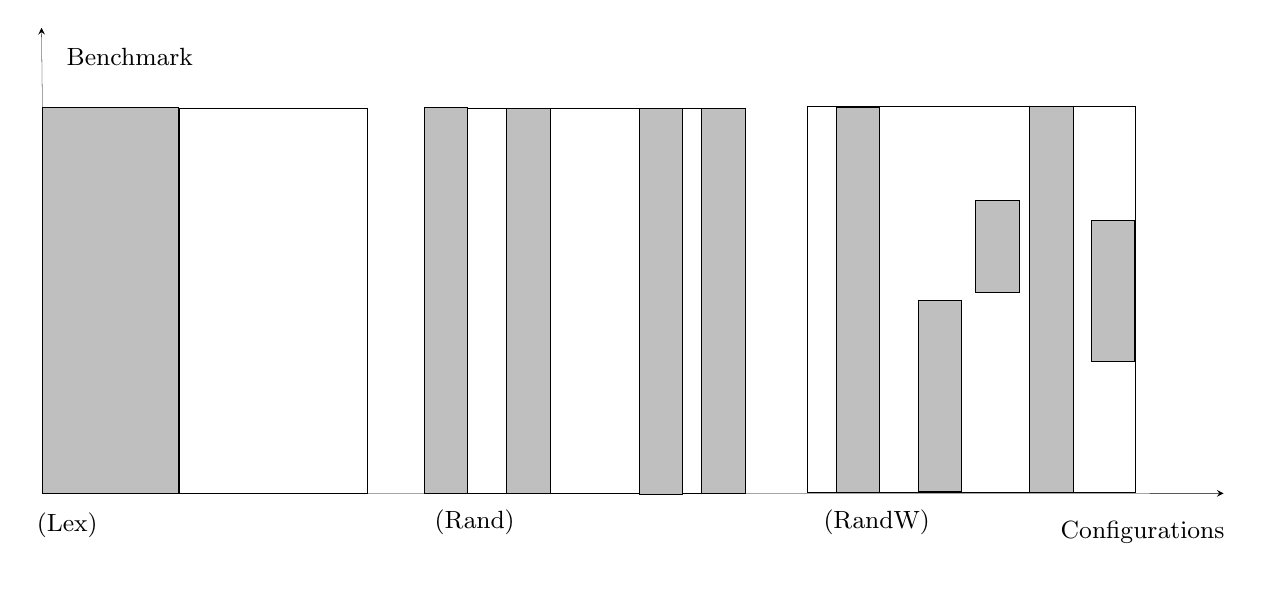
\begin{tikzpicture}
\pgftransformxscale{.5000000}
\pgftransformyscale{-.5000000}
\definecolor{dialinecolor}{rgb}{0.000000, 0.000000, 0.000000}
\pgfsetstrokecolor{dialinecolor}
\definecolor{dialinecolor}{rgb}{1.000000, 1.000000, 1.000000}
\pgfsetfillcolor{dialinecolor}
\definecolor{dialinecolor}{rgb}{0.749020, 0.749020, 0.749020}
\pgfsetfillcolor{dialinecolor}
\fill (15.450000\du,4.950000\du)--(15.450000\du,14.750000\du)--(18.900000\du,14.750000\du)--(18.900000\du,4.950000\du)--cycle;
\pgfsetlinewidth{0.100000\du}
\pgfsetdash{}{0pt}
\pgfsetdash{}{0pt}
\pgfsetmiterjoin
\definecolor{dialinecolor}{rgb}{0.000000, 0.000000, 0.000000}
\pgfsetstrokecolor{dialinecolor}
\draw (15.450000\du,4.950000\du)--(15.450000\du,14.750000\du)--(18.900000\du,14.750000\du)--(18.900000\du,4.950000\du)--cycle;
% setfont left to latex
\definecolor{dialinecolor}{rgb}{0.000000, 0.000000, 0.000000}
\pgfsetstrokecolor{dialinecolor}
\node at (17.175000\du,10.045000\du){};
\definecolor{dialinecolor}{rgb}{1.000000, 1.000000, 1.000000}
\pgfsetfillcolor{dialinecolor}
\fill (18.910000\du,4.955000\du)--(18.910000\du,14.755000\du)--(23.700000\du,14.755000\du)--(23.700000\du,4.955000\du)--cycle;
\pgfsetlinewidth{0.100000\du}
\pgfsetdash{}{0pt}
\pgfsetdash{}{0pt}
\pgfsetmiterjoin
\definecolor{dialinecolor}{rgb}{0.000000, 0.000000, 0.000000}
\pgfsetstrokecolor{dialinecolor}
\draw (18.910000\du,4.955000\du)--(18.910000\du,14.755000\du)--(23.700000\du,14.755000\du)--(23.700000\du,4.955000\du)--cycle;
% setfont left to latex
\definecolor{dialinecolor}{rgb}{0.000000, 0.000000, 0.000000}
\pgfsetstrokecolor{dialinecolor}
\node at (21.305000\du,10.050000\du){};
\pgfsetlinewidth{0.100000\du}
\pgfsetdash{}{0pt}
\pgfsetdash{}{0pt}
\pgfsetbuttcap
{
\definecolor{dialinecolor}{rgb}{0.000000, 0.000000, 0.000000}
\pgfsetfillcolor{dialinecolor}
% was here!!!
\pgfsetarrowsend{stealth}
\definecolor{dialinecolor}{rgb}{0.000000, 0.000000, 0.000000}
\pgfsetstrokecolor{dialinecolor}
\draw (15.450000\du,5.275000\du)--(15.426300\du,2.925000\du);
}
\definecolor{dialinecolor}{rgb}{0.749020, 0.749020, 0.749020}
\pgfsetfillcolor{dialinecolor}
\fill (25.135000\du,4.950000\du)--(25.135000\du,14.750000\du)--(26.235000\du,14.750000\du)--(26.235000\du,4.950000\du)--cycle;
\pgfsetlinewidth{0.100000\du}
\pgfsetdash{}{0pt}
\pgfsetdash{}{0pt}
\pgfsetmiterjoin
\definecolor{dialinecolor}{rgb}{0.000000, 0.000000, 0.000000}
\pgfsetstrokecolor{dialinecolor}
\draw (25.135000\du,4.950000\du)--(25.135000\du,14.750000\du)--(26.235000\du,14.750000\du)--(26.235000\du,4.950000\du)--cycle;
% setfont left to latex
\definecolor{dialinecolor}{rgb}{0.000000, 0.000000, 0.000000}
\pgfsetstrokecolor{dialinecolor}
\node at (25.685000\du,10.045000\du){};
\definecolor{dialinecolor}{rgb}{1.000000, 1.000000, 1.000000}
\pgfsetfillcolor{dialinecolor}
\fill (26.225000\du,4.955000\du)--(26.225000\du,14.755000\du)--(33.225000\du,14.755000\du)--(33.225000\du,4.955000\du)--cycle;
\pgfsetlinewidth{0.100000\du}
\pgfsetdash{}{0pt}
\pgfsetdash{}{0pt}
\pgfsetmiterjoin
\definecolor{dialinecolor}{rgb}{0.000000, 0.000000, 0.000000}
\pgfsetstrokecolor{dialinecolor}
\draw (26.225000\du,4.955000\du)--(26.225000\du,14.755000\du)--(33.225000\du,14.755000\du)--(33.225000\du,4.955000\du)--cycle;
% setfont left to latex
\definecolor{dialinecolor}{rgb}{0.000000, 0.000000, 0.000000}
\pgfsetstrokecolor{dialinecolor}
\node at (29.725000\du,10.050000\du){};
\pgfsetlinewidth{0.100000\du}
\pgfsetdash{}{0pt}
\pgfsetdash{}{0pt}
\pgfsetbuttcap
{
\definecolor{dialinecolor}{rgb}{0.000000, 0.000000, 0.000000}
\pgfsetfillcolor{dialinecolor}
% was here!!!
\pgfsetarrowsend{stealth}
\definecolor{dialinecolor}{rgb}{0.000000, 0.000000, 0.000000}
\pgfsetstrokecolor{dialinecolor}
\draw (23.700000\du,14.755000\du)--(45.451300\du,14.750000\du);
}
\definecolor{dialinecolor}{rgb}{0.749020, 0.749020, 0.749020}
\pgfsetfillcolor{dialinecolor}
\fill (27.235000\du,4.955000\du)--(27.235000\du,14.755000\du)--(28.335000\du,14.755000\du)--(28.335000\du,4.955000\du)--cycle;
\pgfsetlinewidth{0.100000\du}
\pgfsetdash{}{0pt}
\pgfsetdash{}{0pt}
\pgfsetmiterjoin
\definecolor{dialinecolor}{rgb}{0.000000, 0.000000, 0.000000}
\pgfsetstrokecolor{dialinecolor}
\draw (27.235000\du,4.955000\du)--(27.235000\du,14.755000\du)--(28.335000\du,14.755000\du)--(28.335000\du,4.955000\du)--cycle;
% setfont left to latex
\definecolor{dialinecolor}{rgb}{0.000000, 0.000000, 0.000000}
\pgfsetstrokecolor{dialinecolor}
\node at (27.785000\du,10.050000\du){};
\definecolor{dialinecolor}{rgb}{0.749020, 0.749020, 0.749020}
\pgfsetfillcolor{dialinecolor}
\fill (32.185000\du,4.955000\du)--(32.185000\du,14.755000\du)--(33.285000\du,14.755000\du)--(33.285000\du,4.955000\du)--cycle;
\pgfsetlinewidth{0.100000\du}
\pgfsetdash{}{0pt}
\pgfsetdash{}{0pt}
\pgfsetmiterjoin
\definecolor{dialinecolor}{rgb}{0.000000, 0.000000, 0.000000}
\pgfsetstrokecolor{dialinecolor}
\draw (32.185000\du,4.955000\du)--(32.185000\du,14.755000\du)--(33.285000\du,14.755000\du)--(33.285000\du,4.955000\du)--cycle;
% setfont left to latex
\definecolor{dialinecolor}{rgb}{0.000000, 0.000000, 0.000000}
\pgfsetstrokecolor{dialinecolor}
\node at (32.735000\du,10.050000\du){};
\definecolor{dialinecolor}{rgb}{0.749020, 0.749020, 0.749020}
\pgfsetfillcolor{dialinecolor}
\fill (30.595000\du,4.960000\du)--(30.595000\du,14.760000\du)--(31.695000\du,14.760000\du)--(31.695000\du,4.960000\du)--cycle;
\pgfsetlinewidth{0.100000\du}
\pgfsetdash{}{0pt}
\pgfsetdash{}{0pt}
\pgfsetmiterjoin
\definecolor{dialinecolor}{rgb}{0.000000, 0.000000, 0.000000}
\pgfsetstrokecolor{dialinecolor}
\draw (30.595000\du,4.960000\du)--(30.595000\du,14.760000\du)--(31.695000\du,14.760000\du)--(31.695000\du,4.960000\du)--cycle;
% setfont left to latex
\definecolor{dialinecolor}{rgb}{0.000000, 0.000000, 0.000000}
\pgfsetstrokecolor{dialinecolor}
\node at (31.145000\du,10.055000\du){};
\definecolor{dialinecolor}{rgb}{1.000000, 1.000000, 1.000000}
\pgfsetfillcolor{dialinecolor}
\fill (34.876300\du,4.915000\du)--(34.876300\du,14.715000\du)--(43.196300\du,14.715000\du)--(43.196300\du,4.915000\du)--cycle;
\pgfsetlinewidth{0.100000\du}
\pgfsetdash{}{0pt}
\pgfsetdash{}{0pt}
\pgfsetmiterjoin
\definecolor{dialinecolor}{rgb}{0.000000, 0.000000, 0.000000}
\pgfsetstrokecolor{dialinecolor}
\draw (34.876300\du,4.915000\du)--(34.876300\du,14.715000\du)--(43.196300\du,14.715000\du)--(43.196300\du,4.915000\du)--cycle;
% setfont left to latex
\definecolor{dialinecolor}{rgb}{0.000000, 0.000000, 0.000000}
\pgfsetstrokecolor{dialinecolor}
\node at (39.036300\du,10.010000\du){};
% setfont left to latex
\definecolor{dialinecolor}{rgb}{0.000000, 0.000000, 0.000000}
\pgfsetstrokecolor{dialinecolor}
\node[anchor=west] at (20.801300\du,16.225000\du){};
% setfont left to latex
\definecolor{dialinecolor}{rgb}{0.000000, 0.000000, 0.000000}
\pgfsetstrokecolor{dialinecolor}
\node[anchor=west] at (41.076300\du,15.750000\du){\small  Configurations};
% setfont left to latex
\definecolor{dialinecolor}{rgb}{0.000000, 0.000000, 0.000000}
\pgfsetstrokecolor{dialinecolor}
\node[anchor=west] at (15.826300\du,3.675000\du){\small  Benchmark};
% setfont left to latex
\definecolor{dialinecolor}{rgb}{0.000000, 0.000000, 0.000000}
\pgfsetstrokecolor{dialinecolor}
\node[anchor=west] at (15.070700\du,15.550000\du){ \small  (Lex)};
% setfont left to latex
\definecolor{dialinecolor}{rgb}{0.000000, 0.000000, 0.000000}
\pgfsetstrokecolor{dialinecolor}
\node[anchor=west] at (25.175000\du,15.475000\du){\small  (Rand)};
% setfont left to latex
\definecolor{dialinecolor}{rgb}{0.000000, 0.000000, 0.000000}
\pgfsetstrokecolor{dialinecolor}
\node[anchor=west] at (35.050700\du,15.485000\du){\small  (RandW)};
% setfont left to latex
\definecolor{dialinecolor}{rgb}{0.000000, 0.000000, 0.000000}
\pgfsetstrokecolor{dialinecolor}
\node[anchor=west] at (18.800000\du,15.100000\du){};
\definecolor{dialinecolor}{rgb}{0.749020, 0.749020, 0.749020}
\pgfsetfillcolor{dialinecolor}
\fill (35.610000\du,4.930000\du)--(35.610000\du,14.730000\du)--(36.710000\du,14.730000\du)--(36.710000\du,4.930000\du)--cycle;
\pgfsetlinewidth{0.100000\du}
\pgfsetdash{}{0pt}
\pgfsetdash{}{0pt}
\pgfsetmiterjoin
\definecolor{dialinecolor}{rgb}{0.000000, 0.000000, 0.000000}
\pgfsetstrokecolor{dialinecolor}
\draw (35.610000\du,4.930000\du)--(35.610000\du,14.730000\du)--(36.710000\du,14.730000\du)--(36.710000\du,4.930000\du)--cycle;
% setfont left to latex
\definecolor{dialinecolor}{rgb}{0.000000, 0.000000, 0.000000}
\pgfsetstrokecolor{dialinecolor}
\node at (36.160000\du,10.025000\du){};
\definecolor{dialinecolor}{rgb}{0.749020, 0.749020, 0.749020}
\pgfsetfillcolor{dialinecolor}
\fill (40.520000\du,4.910000\du)--(40.520000\du,14.710000\du)--(41.620000\du,14.710000\du)--(41.620000\du,4.910000\du)--cycle;
\pgfsetlinewidth{0.100000\du}
\pgfsetdash{}{0pt}
\pgfsetdash{}{0pt}
\pgfsetmiterjoin
\definecolor{dialinecolor}{rgb}{0.000000, 0.000000, 0.000000}
\pgfsetstrokecolor{dialinecolor}
\draw (40.520000\du,4.910000\du)--(40.520000\du,14.710000\du)--(41.620000\du,14.710000\du)--(41.620000\du,4.910000\du)--cycle;
% setfont left to latex
\definecolor{dialinecolor}{rgb}{0.000000, 0.000000, 0.000000}
\pgfsetstrokecolor{dialinecolor}
\node at (41.070000\du,10.005000\du){};
\definecolor{dialinecolor}{rgb}{0.749020, 0.749020, 0.749020}
\pgfsetfillcolor{dialinecolor}
\fill (37.680000\du,9.850000\du)--(37.680000\du,14.700000\du)--(38.780000\du,14.700000\du)--(38.780000\du,9.850000\du)--cycle;
\pgfsetlinewidth{0.100000\du}
\pgfsetdash{}{0pt}
\pgfsetdash{}{0pt}
\pgfsetmiterjoin
\definecolor{dialinecolor}{rgb}{0.000000, 0.000000, 0.000000}
\pgfsetstrokecolor{dialinecolor}
\draw (37.680000\du,9.850000\du)--(37.680000\du,14.700000\du)--(38.780000\du,14.700000\du)--(38.780000\du,9.850000\du)--cycle;
% setfont left to latex
\definecolor{dialinecolor}{rgb}{0.000000, 0.000000, 0.000000}
\pgfsetstrokecolor{dialinecolor}
\node at (38.230000\du,12.470000\du){};
\definecolor{dialinecolor}{rgb}{0.749020, 0.749020, 0.749020}
\pgfsetfillcolor{dialinecolor}
\fill (42.090000\du,7.800000\du)--(42.090000\du,11.400000\du)--(43.190000\du,11.400000\du)--(43.190000\du,7.800000\du)--cycle;
\pgfsetlinewidth{0.100000\du}
\pgfsetdash{}{0pt}
\pgfsetdash{}{0pt}
\pgfsetmiterjoin
\definecolor{dialinecolor}{rgb}{0.000000, 0.000000, 0.000000}
\pgfsetstrokecolor{dialinecolor}
\draw (42.090000\du,7.800000\du)--(42.090000\du,11.400000\du)--(43.190000\du,11.400000\du)--(43.190000\du,7.800000\du)--cycle;
% setfont left to latex
\definecolor{dialinecolor}{rgb}{0.000000, 0.000000, 0.000000}
\pgfsetstrokecolor{dialinecolor}
\node at (42.640000\du,9.795000\du){};
\definecolor{dialinecolor}{rgb}{0.749020, 0.749020, 0.749020}
\pgfsetfillcolor{dialinecolor}
\fill (39.150000\du,7.300000\du)--(39.150000\du,9.650000\du)--(40.250000\du,9.650000\du)--(40.250000\du,7.300000\du)--cycle;
\pgfsetlinewidth{0.100000\du}
\pgfsetdash{}{0pt}
\pgfsetdash{}{0pt}
\pgfsetmiterjoin
\definecolor{dialinecolor}{rgb}{0.000000, 0.000000, 0.000000}
\pgfsetstrokecolor{dialinecolor}
\draw (39.150000\du,7.300000\du)--(39.150000\du,9.650000\du)--(40.250000\du,9.650000\du)--(40.250000\du,7.300000\du)--cycle;
% setfont left to latex
\definecolor{dialinecolor}{rgb}{0.000000, 0.000000, 0.000000}
\pgfsetstrokecolor{dialinecolor}
\node at (39.700000\du,8.670000\du){};
\end{tikzpicture}

	%}
	\caption{Lexicographic, random and random oracle with wisdom.
        {\it Lex} explores the search space in the lexicographic order. {\it Rand}  and {\it RandW} 
        randomly choose the next configuration. {\it RandW} differs from {\it Rand} on the fact that 
        it extracts information from configurations that were partially explored.}
	\label{fig:Search}
	\end{center}
	\end{figure}


\subsubsection{A similarity approach for finding hard instances.}  

The main assumption we made for detecting hard instances is that their
{\it runtime will look similar on the configurations we processed}.
Let us assume at the date $t$ that we processed the set of
configurations $\Theta(t)$. Let us also assume that there is a subset
$\Theta_1(t) \subseteq \Theta(t)$ for which the evaluations were
performed on all $B$~\footnote{due to lower bound elimination we could
  stricly have $\Theta(t) \setminus \Theta_1(t) \neq \emptyset$}.  We
propose to characterize the runtime of each instance $\beta \in B$ as
a vector
\[ \Delta(\beta) = [\Delta(\sigma, \bar{\theta^{'}_0}, \beta), \dots
\Delta(\sigma, \bar{\theta^{'}_{n_1}}, \beta) ]^T \]
where $n_1 = |\Theta_1(t)|$. Here, $\theta^{'}_{i}$ are configurations
in $\Theta_1(t)$ that we ordered randomly.

In other words, the runtime vector of a benchmark entry is the
collection of runtimes we observed on $\Theta_1(t)$.  Given these
data, we propose to apply a $2-$Means clustering algorithm on the data
$B$ with the runtime vector and the euclidian distance. Finally, we
conclude that hard instances are those, in the class, for which the
mean value $\norm{\Delta(\beta)}$ is the greatest. Indeed, it is
intuitive to expect that on hard instances, most configurations take a
huge runtime before finding the optimal solution.

Let us mention that the idea of distinguishing hard instances of
NP-hard problem with a machine learning approach was also investigated
in another paper~\cite{WZZReport}. But our approach completely differs
from this proposition on the modeling of features.  The {\it Rand}
oracle uses the result update process of {\it Lex}. However, it is
based on a deeper exploitation of the potential random distribution of
best configurations. In addition, it exploits more past information
generated in the exploration to take further decisions. But, this
point could be improved as we will see in the sequel.

\subsection{Random oracle with the wisdom of the loosers (RandW)}

With {\it Rand}, estimations made on $\bar{\theta^{'}_0}$ could serve
to guide the exploration of $\bar{\theta^{'}_{1}}$,
$\bar{\theta^{'}_{2}}$ etc. This extraction of information is
interesting, but there still remains a wastage. Indeed, data related
to the {\it losing configurations}
$\Theta_2(t) = \Theta(t) \setminus \Theta_1(t)$ are not exploited by
the oracle~\footnote{Losing configurations are those on which we did
  not entirely evaluated $B$ because we detected before a lower bound
  violation.}.  This can be seen as a loss if we consider the
processing cost that these evaluations required. The question then is:
how could we exploit {\it this effort} for taking better decisions?

For this purpose, let us come back to the random oracle. At the
begining of the exploration of any configuration $\theta_i$, the
algorithm separates instances in hard and softs. Then, it randomly
chooses instances in the hard class and then the ones of the soft
class. This random choice could be improved in considering data of
losing configurations. For example, beeing given the set hard instance
$B_{hard}$, we could observe from data of the loosers that a small
subset $B_{hard^+}$ of these data was generally enough to reach a
lower bound violation. Then, instead of a random exploration of
$B_{hard}$, it will be more efficient to randomly start by instances
in $B_{hard^+}$.  Globally, we can then reformulate the exploration of
a configuration points as follows. We first start with the benchmark
entries in $B_{hard^+} \cap B_{hard}$, then by the one in
$B_{hard^+} \cap B_{soft}$ and finally the remaining instances in
considering hard instances before soft ones. The question is: how to
build $B_{hard^+}$?


\subsubsection{Computation of hard instances as a subset intersection problem.} 

We propose to consider $B_{hard^+}$ as the set of benchmark entries
for which there is a maximal number of losing configurations that were
evaluated. The idea behind is that the more a same benchmark entry was
evaluated in losing configurations, the more, we could believe that
this benchmark entry causes lower bound violations.

More practically, at each date $t$, we assume that we know the size
$K(t)$ of $B_{hard^+}$ (this will be discussed latter).  For computing
$B_{hard^+}$, we firstly associate each benchmark entry $\beta$ with a
configuration set $S(\beta)$ whose elements are all configurations
$\bar{\theta} \in \Theta_2(t)$ for which there exists a computed
estimation $\Delta(\sigma, \bar{\theta}, \beta)$. We then choose
$B_{hard^+}$ as the set of benchmark entries
$\{ \beta^+_1, \dots, \beta^+_k \}$ such that
$|\{ \beta^+_1, \dots, \beta^+_k \}| = K(t)$ and
$|S(\beta^+_1) \cap \dots \cap S(\beta^+_k)|$ is maximal.


With this formulation, we will decide on the construction of
$B_{hard^+}$ based on
$|S(\beta^+_1) \cap \dots \cap S(\beta^+_k)|.K(t)$ additional data. In
the best case, when comparing with {\it Rand}, we will have
$|\Theta_2(t)|.K(t)$ additional data that {\it we will transform in
  information}.  This formulation has two challenges. The first one is
that we need to tune $K(t)$. In our implementation, we propose to
randomly chose these values. The second challenge is the resolution of
the intersection problem we introduced.

\subsubsection{ Greedy algorithm for computing $B_{hard^+}$.}

One can easily notice that the computation of $B_{hard^+}$, as
formulated, corresponds to the resolution of the Maximum $K$-intersection
problem~\cite{DBLP:journals/ipl/ShiehTY12}.  Indeed, this latter
problem is defined as follows.

Given $n$ sets $E_1,\dots,E_m$ with elements over a universe
$\Sigma = \{ e_1,\dots,e_n  \}$, the goal is to select $K$ subsets of
$E_1,\dots,E_m$ in order to maximize the size of the intersection of
the sets.  As shown in~\cite{DBLP:journals/ipl/ShiehTY12}, this
problem is NP-complete and cannot be approximated within an absolute
error of $\frac{1}{2}n^{1-2\epsilon} + \frac{3}{8}n^{1-3\epsilon} - 1$
unless {\bf P = NP}.  However this intersection problem is close to
coverage problems for which there exists a general heuristic
framework. The first stage in this framework consists in ordering the
sets $S(\beta)$ according to a pricing strategy. Then, the sets with
higher prices are progressively chosen until we reach a subset
intersection that cannot evolve. Using this idea, we propose in
Algorithm~\ref{alg4} a greedy solution for building the $B_{hard^+}$
set.

	\begin{algorithm}                    
	\caption{\scriptsize RandW Hard instance selection (RandW-HIS)} 	\label{alg4}  
	\begin{algorithmic}[1]
	\scriptsize
	\FOR{$\beta \in \Theta_2(t)$}
	\STATE Build the set $S(\beta)$.
	\ENDFOR
	\STATE $C = \emptyset$; $Inter = \Theta_2(t)$
	\WHILE{$|C| < K(t)$}
		\STATE Choose the set $S(\beta)$ s.t. $S(\beta)$ is not in $C$ and $|S(\beta) \cap Inter|$ is maximal;
		\STATE $C  = C \cup S(\beta)$
                \STATE $Inter = Inter \cap S(\beta)$
	\ENDWHILE
	\STATE return $C$
	\end{algorithmic}
	\end{algorithm}
	\normalsize

        We end here the description of the data exploration and
        exploitation in QTuning. The next section is devoted to
        experiments.


\section{Experimental evaluation} \label{Proof-of-concept}

\subsection{Settings}
In considering the architecture of Figure~\ref{fig:QTuning}, we simulated the behavior of 
the active learning framework in a setting where given a tuning project pushed at date $0$,  
{\it service.d} requested a new configuration to {\it QTunind.d} every $d$ seconds. 
We assume that between these $d$ seconds, the active learning framework was able to launch exploration 
jobs and get the results on $p$ configuration points. For obtaining the $p$ points, the framework 
could have used the oracles above.
\begin{itemize}
\item {\it lex:} it corresponds to the {\it Lex} oracle.
\item {\it rand:} the {\it Rand} oracle;
\item {\it rand\_sort:} the {\it Rand} oracle; but the group of hard and soft instances are each sorted in ascending order on the value of $\norm{\Delta(\beta)}$;
\item {\it rand\_desc\_sort:} the {\it Rand} oracle; but each group of hard and soft instance is sorted in descending order on the value of $\norm{\Delta(\beta)}$;
\item {\it rand\_w:} the {\it RandW} oracle;
\item {\it rand\_w\_noh:} the {\it RandW} oracle; but we choose $B_{hard}$ randomly instead of using the $2$-Means clustering.
\end{itemize}

For evaluating the oracles, we assumed three tuning projects based on the data of an international SAT 
competition~\footnote{http://satcompetition.org/edacc/SATCompetition2013/}. In this competition, various 
solvers are evaluated on instances of the NP-hard problem SAT. The benchmark 
instances $B$ and the configurations $\Theta$ of each tuning project are associated 
with a sub-competition. In each sub-competition, we fixed the values $\Delta(\sigma, \bar{\theta_i}, \beta_j)$ as the 
runtime of a SAT solver on a benchmark instance. Let us notice that all these runtime are available 
in the competition web site. Finally, the chosen sub-competitions are: Core solvers sequential on random satisfiable+unsatisfiable instances (c-SAT+UNSAT), Core solvers sequential on satisfiable instances (c-SAT) and  Core solvers sequential on hard satisfiable+unsatisfiable instances (c-SAT+UNSAT|Hard). 

\subsection{Experimental plan}

We did $7$ series of experiments. In each, we computed the regret of the active learning framewok for each 
of the oracles in a discrete windows of time $t_0,\dots ,t_n$. 
For the first $3$ experiments, all oracles were evaluated assuming data of three sub-competitions. The 
evaluation for each competition included $300$ sub-evaluations, were we changed the ordering of instances $B$ and 
configurations $\Theta$.  The objective in these first experiments was to find the best oracle. In experiment $4$, we 
compared variants of the {\it Randw} with different values of  $K(t)$. Finally, in experiments, 
$5$, $6$ and $7$, we compared all the oracles when the values of $p$ are changed. The experiments plan 
are summarized in Table~\ref{tab:plan}

\begin{table}
  \begin{center}
  \begin{tabular}{ p{1cm} | p{6cm} }

    {\small Exp.1} & {\small competition=c-SAT+UNSAT ($|B| = 300$, $|\Theta| = 28$), $d=600$, $p=100$, $t_0 = 0$, $t_n = 76.d$, $K(t) = 10$} \\\hline
    {\small Exp.2} & {\small competition=c-SAT ($|B| = 300$, $|\Theta| = 31$), $d=600$, $p=100$, $t_0 = 0$, $t_n = 45.d$, $K(t) = 10$} \\\hline
    {\small Exp.3} & {\small competition=c-SAT+UNSAT|Hard ($|B| = 300$, $|\Theta| = 31$), $d=600$, $p=100$, $t_0 = 0$, $t_n = 92.d$, $K(t) = 10$} \\\hline
    {\small Exp.4} & {\small competition=c-SAT+UNSAT, $d=600$, $p=100$, $t_0 = 0$, $t_n = 76.d$, $K(t) = 10, 20, 30, 40$} \\\hline
    {\small Exp.5} & {\small competition=c-SAT+UNSAT, $d=600$, $p=120$, $t_0 = 0$, $t_n = 76.d$, $K(t) = 10$} \\\hline
    {\small Exp.6} & {\small competition=c-SAT+UNSAT, $d=600$, $p=140$, $t_0 = 0$, $t_n = 76.d$, $K(t) = 10$} \\\hline
    {\small Exp.7} & {\small competition=c-SAT+UNSAT, $d=600$, $p=160$, $t_0 = 0$, $t_n = 76.d$, $K(t) = 10$} \\
  \end{tabular}
  \caption{Experimental plan}
  \label{tab:plan}
  \end{center} 
\end{table}




\subsection{Experimental results and analysis}

In Figure~\ref{fig:regret}, we present the mean regret we obtained. The first lesson we learn is that 
on {\small Exp.1, Exp.2, Exp.3}, the best oracle is {\it rand\_desc\_sort}  and the worst is {\it lex}. 
Indeed, this oracle leads to the minimal regret within the time. In the plots in Figure~\ref{fig:regret}, 
one can notice that the regret starts to grow quiclky and then stabilizes. This is normal since within 
the time, we are approaching the optimal solution. 
These first experiments confirm two noticeable points: the interest of randomization 
for regret minimization ({\it lex} is the worst oracle) and the interest in processing instances with hard ones 
before soft ones instances. 

The oracle {\it rand\_desc\_sort} was either followed by {\it rand}, or by {\it rand\_w} and its variant. 
This means that there is an interest in using the wisdom of the loser. Since in the first experiments, 
we set $K(t)$ to $10$, a question was then to see whether or not we could obtain better 
results for {\it wisdom of loser oracles} in changing the $K(t)$.  The answer for this question is yes. 
As shown in {\small Exp.4} there is an effective 
performance variation when $K(t)$ is changed. Consequently, for further work it is interesting to invest on how to 
decide the best value of $K(t)$. Finally, in the figures~\ref{fig:regret}(e-f), we present what we obtained in changing 
the number of configuration points that we processed between the $d$ seconds. The results confirm the trend we observed 
in the three first experiments. 


\begin{figure*}[ht]
\centering
\subfloat[{\scriptsize Exp.1}]{
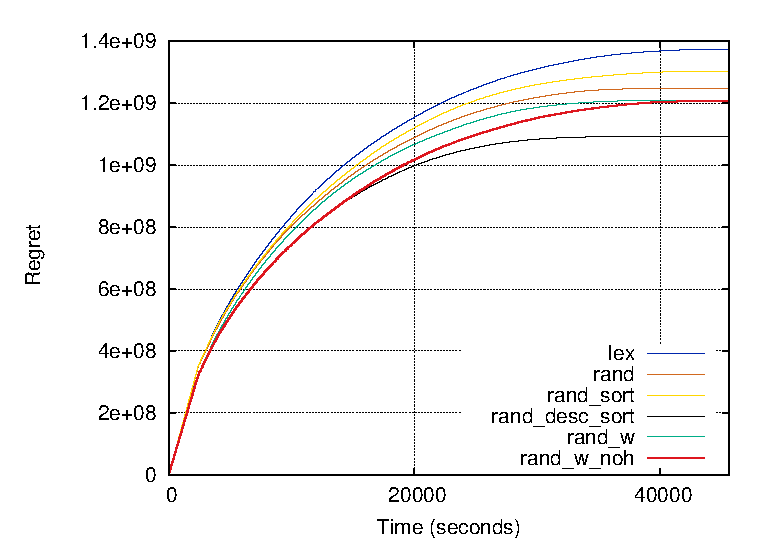
\includegraphics[scale=0.6]{./Figures/exp1.eps}
}
\subfloat[{\scriptsize Exp.2}]{
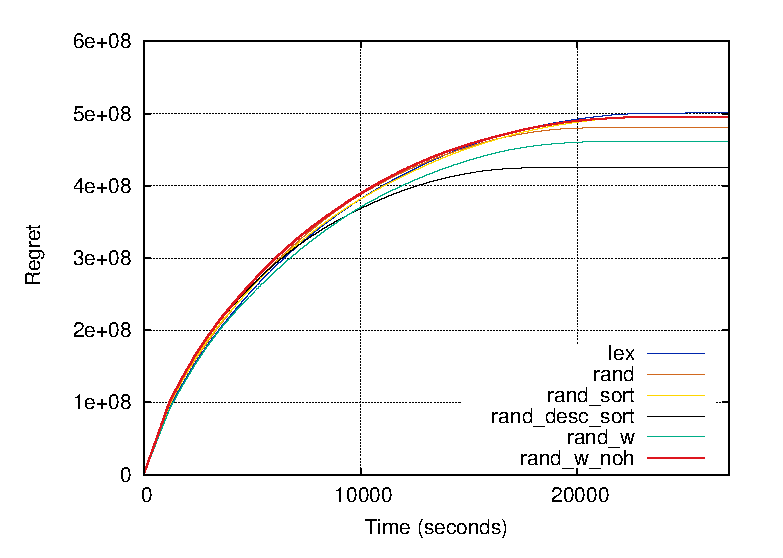
\includegraphics[scale=0.6]{./Figures/exp2.eps}
}
\\
\subfloat[{\scriptsize Exp.3}]{
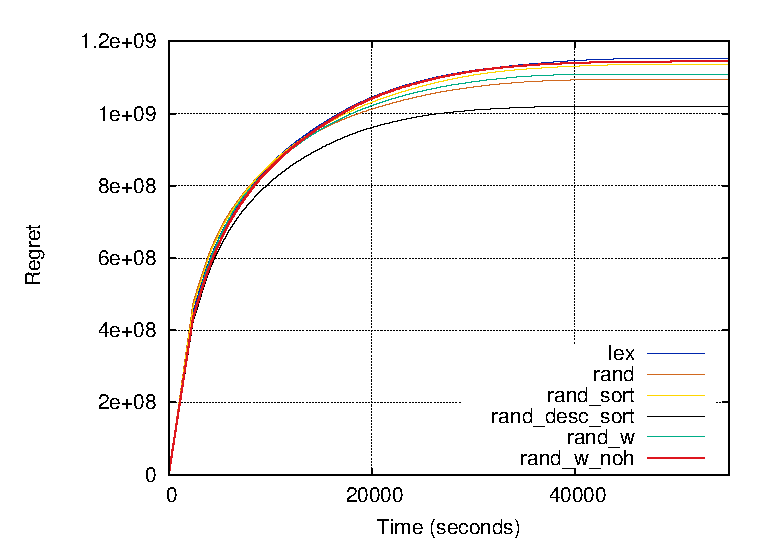
\includegraphics[scale=0.6]{./Figures/exp3.eps}
}
\subfloat[{\scriptsize Exp.4}]{
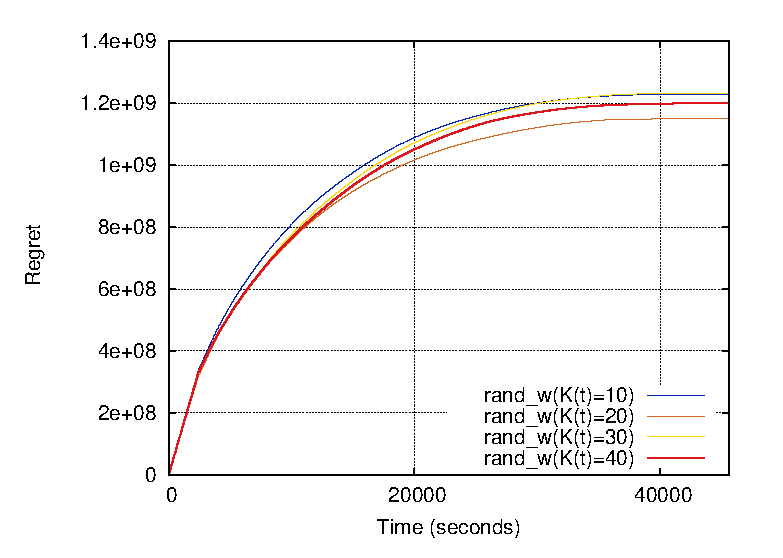
\includegraphics[scale=0.6]{./Figures/exp4.eps}
}
\\
\subfloat[{\scriptsize Exp.5}]{
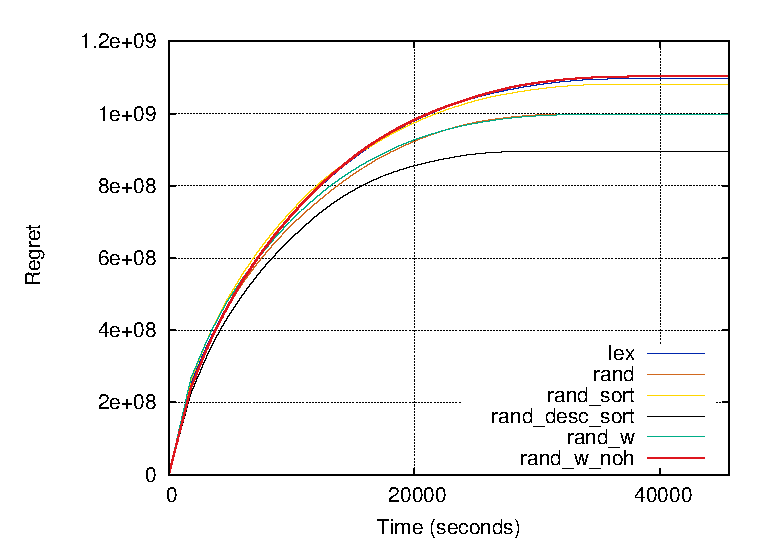
\includegraphics[scale=0.6]{./Figures/exp5.eps}
}
\subfloat[{\scriptsize Exp.6}]{
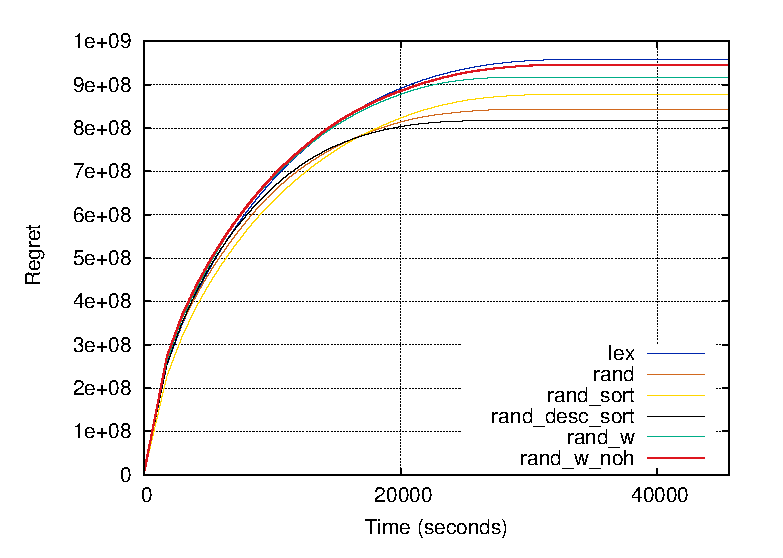
\includegraphics[scale=0.6]{./Figures/exp6.eps}
}
\\
\subfloat[{\scriptsize Exp.7}]{
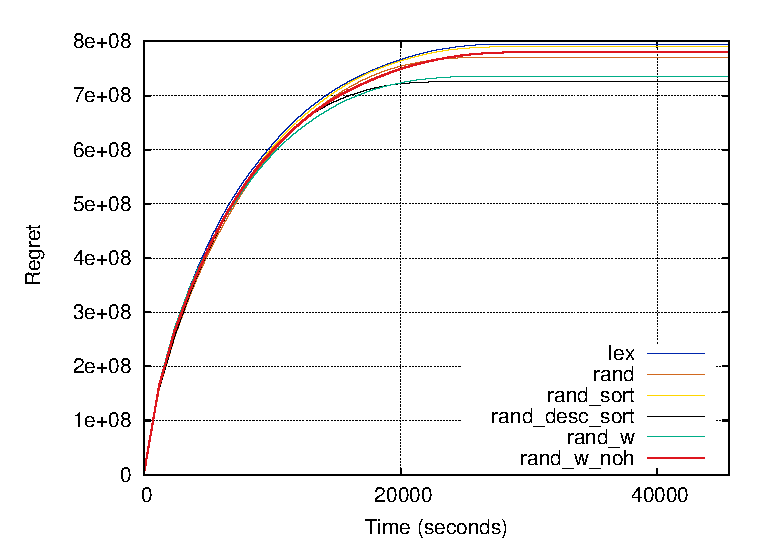
\includegraphics[scale=0.6]{./Figures/exp7.eps}
}

\caption{Mean regret obtained from the experiments whose settings are in Table~\ref{tab:plan}}
\label{fig:regret}
\end{figure*}

\section{Conclusion} \label{Conclusion}

In this paper, we introduced a new automatic tuning system for NP-hard algorithms in a cloud 
context. The proposed system is based on an active learning framework where we continuously 
learn the best configuration while servicing cloud requests with the best local results found. 
We proposed a naive oracle for the learning process and several  
 improvements based on randomization, k-means clustering and the resolution of a set intersection problem. 
We then simulate the performance of our oracles based on runtime of algorithms solving the satisfiability 
problem. The experiments clearly demonstrated that our improved oracles are better in the practice. 
They also reveal the dominance of some oracles. 

For continuing this work, we envision three main perspectives. The first one is to combine the different 
oracles in a general active learning framework. Here, we could 
use for example multi-armed bandit models. Our second perspective is to refine the classification of hard 
instances such as to define better techniques for ordering configuration points. Indeed, the experiments showed  
that the usage of sorting or the wisdom of the losers can improve the {\it Rand} oracle. Finally, we intend 
to define {\it filling techniques} such as to predict the value of configuration points with few processing. 
We do believe that given an instance, from the trace execution of a set of configurations on it,  we can estimate the runtime 
it will have on new configuration.

\bibliographystyle{./IEEEtran}
\bibliography{self_learning}




% that's all folks
\end{document}

